% Options for packages loaded elsewhere
\PassOptionsToPackage{unicode}{hyperref}
\PassOptionsToPackage{hyphens}{url}
%
\documentclass[
]{book}
\usepackage{amsmath,amssymb}
\usepackage{iftex}
\ifPDFTeX
  \usepackage[T1]{fontenc}
  \usepackage[utf8]{inputenc}
  \usepackage{textcomp} % provide euro and other symbols
\else % if luatex or xetex
  \usepackage{unicode-math} % this also loads fontspec
  \defaultfontfeatures{Scale=MatchLowercase}
  \defaultfontfeatures[\rmfamily]{Ligatures=TeX,Scale=1}
\fi
\usepackage{lmodern}
\ifPDFTeX\else
  % xetex/luatex font selection
\fi
% Use upquote if available, for straight quotes in verbatim environments
\IfFileExists{upquote.sty}{\usepackage{upquote}}{}
\IfFileExists{microtype.sty}{% use microtype if available
  \usepackage[]{microtype}
  \UseMicrotypeSet[protrusion]{basicmath} % disable protrusion for tt fonts
}{}
\makeatletter
\@ifundefined{KOMAClassName}{% if non-KOMA class
  \IfFileExists{parskip.sty}{%
    \usepackage{parskip}
  }{% else
    \setlength{\parindent}{0pt}
    \setlength{\parskip}{6pt plus 2pt minus 1pt}}
}{% if KOMA class
  \KOMAoptions{parskip=half}}
\makeatother
\usepackage{xcolor}
\usepackage{color}
\usepackage{fancyvrb}
\newcommand{\VerbBar}{|}
\newcommand{\VERB}{\Verb[commandchars=\\\{\}]}
\DefineVerbatimEnvironment{Highlighting}{Verbatim}{commandchars=\\\{\}}
% Add ',fontsize=\small' for more characters per line
\usepackage{framed}
\definecolor{shadecolor}{RGB}{248,248,248}
\newenvironment{Shaded}{\begin{snugshade}}{\end{snugshade}}
\newcommand{\AlertTok}[1]{\textcolor[rgb]{0.94,0.16,0.16}{#1}}
\newcommand{\AnnotationTok}[1]{\textcolor[rgb]{0.56,0.35,0.01}{\textbf{\textit{#1}}}}
\newcommand{\AttributeTok}[1]{\textcolor[rgb]{0.13,0.29,0.53}{#1}}
\newcommand{\BaseNTok}[1]{\textcolor[rgb]{0.00,0.00,0.81}{#1}}
\newcommand{\BuiltInTok}[1]{#1}
\newcommand{\CharTok}[1]{\textcolor[rgb]{0.31,0.60,0.02}{#1}}
\newcommand{\CommentTok}[1]{\textcolor[rgb]{0.56,0.35,0.01}{\textit{#1}}}
\newcommand{\CommentVarTok}[1]{\textcolor[rgb]{0.56,0.35,0.01}{\textbf{\textit{#1}}}}
\newcommand{\ConstantTok}[1]{\textcolor[rgb]{0.56,0.35,0.01}{#1}}
\newcommand{\ControlFlowTok}[1]{\textcolor[rgb]{0.13,0.29,0.53}{\textbf{#1}}}
\newcommand{\DataTypeTok}[1]{\textcolor[rgb]{0.13,0.29,0.53}{#1}}
\newcommand{\DecValTok}[1]{\textcolor[rgb]{0.00,0.00,0.81}{#1}}
\newcommand{\DocumentationTok}[1]{\textcolor[rgb]{0.56,0.35,0.01}{\textbf{\textit{#1}}}}
\newcommand{\ErrorTok}[1]{\textcolor[rgb]{0.64,0.00,0.00}{\textbf{#1}}}
\newcommand{\ExtensionTok}[1]{#1}
\newcommand{\FloatTok}[1]{\textcolor[rgb]{0.00,0.00,0.81}{#1}}
\newcommand{\FunctionTok}[1]{\textcolor[rgb]{0.13,0.29,0.53}{\textbf{#1}}}
\newcommand{\ImportTok}[1]{#1}
\newcommand{\InformationTok}[1]{\textcolor[rgb]{0.56,0.35,0.01}{\textbf{\textit{#1}}}}
\newcommand{\KeywordTok}[1]{\textcolor[rgb]{0.13,0.29,0.53}{\textbf{#1}}}
\newcommand{\NormalTok}[1]{#1}
\newcommand{\OperatorTok}[1]{\textcolor[rgb]{0.81,0.36,0.00}{\textbf{#1}}}
\newcommand{\OtherTok}[1]{\textcolor[rgb]{0.56,0.35,0.01}{#1}}
\newcommand{\PreprocessorTok}[1]{\textcolor[rgb]{0.56,0.35,0.01}{\textit{#1}}}
\newcommand{\RegionMarkerTok}[1]{#1}
\newcommand{\SpecialCharTok}[1]{\textcolor[rgb]{0.81,0.36,0.00}{\textbf{#1}}}
\newcommand{\SpecialStringTok}[1]{\textcolor[rgb]{0.31,0.60,0.02}{#1}}
\newcommand{\StringTok}[1]{\textcolor[rgb]{0.31,0.60,0.02}{#1}}
\newcommand{\VariableTok}[1]{\textcolor[rgb]{0.00,0.00,0.00}{#1}}
\newcommand{\VerbatimStringTok}[1]{\textcolor[rgb]{0.31,0.60,0.02}{#1}}
\newcommand{\WarningTok}[1]{\textcolor[rgb]{0.56,0.35,0.01}{\textbf{\textit{#1}}}}
\usepackage{longtable,booktabs,array}
\usepackage{calc} % for calculating minipage widths
% Correct order of tables after \paragraph or \subparagraph
\usepackage{etoolbox}
\makeatletter
\patchcmd\longtable{\par}{\if@noskipsec\mbox{}\fi\par}{}{}
\makeatother
% Allow footnotes in longtable head/foot
\IfFileExists{footnotehyper.sty}{\usepackage{footnotehyper}}{\usepackage{footnote}}
\makesavenoteenv{longtable}
\usepackage{graphicx}
\makeatletter
\def\maxwidth{\ifdim\Gin@nat@width>\linewidth\linewidth\else\Gin@nat@width\fi}
\def\maxheight{\ifdim\Gin@nat@height>\textheight\textheight\else\Gin@nat@height\fi}
\makeatother
% Scale images if necessary, so that they will not overflow the page
% margins by default, and it is still possible to overwrite the defaults
% using explicit options in \includegraphics[width, height, ...]{}
\setkeys{Gin}{width=\maxwidth,height=\maxheight,keepaspectratio}
% Set default figure placement to htbp
\makeatletter
\def\fps@figure{htbp}
\makeatother
\ifLuaTeX
  \usepackage{luacolor}
  \usepackage[soul]{lua-ul}
\else
  \usepackage{soul}
\fi
\setlength{\emergencystretch}{3em} % prevent overfull lines
\providecommand{\tightlist}{%
  \setlength{\itemsep}{0pt}\setlength{\parskip}{0pt}}
\setcounter{secnumdepth}{5}
\usepackage{booktabs}
\usepackage{longtable}
\usepackage{array}
\usepackage{multirow}
\usepackage{wrapfig}
\usepackage{float}
\usepackage{colortbl}
\usepackage{pdflscape}
\usepackage{tabu}
\usepackage{threeparttable}
\usepackage{threeparttablex}
\usepackage[normalem]{ulem}
\usepackage{makecell}
\usepackage{xcolor}
\ifLuaTeX
  \usepackage{selnolig}  % disable illegal ligatures
\fi
\usepackage[]{natbib}
\bibliographystyle{plainnat}
\usepackage{bookmark}
\IfFileExists{xurl.sty}{\usepackage{xurl}}{} % add URL line breaks if available
\urlstyle{same}
\hypersetup{
  pdftitle={Bioestatística Usando o R},
  pdfauthor={Petrônio Fagundes de Oliveira Filho},
  hidelinks,
  pdfcreator={LaTeX via pandoc}}

\title{Bioestatística Usando o R}
\author{Petrônio Fagundes de Oliveira Filho}
\date{2025-05-02}

\begin{document}
\maketitle

{
\setcounter{tocdepth}{1}
\tableofcontents
}
\chapter{Introdução}\label{introduuxe7uxe3o}

\section{Importância da Bioestatística}\label{importuxe2ncia-da-bioestatuxedstica}

Os indivíduos variam em relação as suas características biológicas, psicológicas e sociais na saúde e na doença. Esta variabilidade gera uma grande quantidade de incertezas.

A Bioestatística, estatística aplicada às ciências biológicas e da saúde, é a ferramenta utilizada pelos pesquisadores para trabalhar com essas incertezas advindas da variabilidade. Várias definições foram escritas para a estatística, uma delas é a seguinte \citep{armitage2008statistical}:

\begin{quote}
Estatística é a disciplina interessada com o tratamento dos dados numéricos obtidos a partir de grupos de indivíduos
\end{quote}

A Bioestatística lida com a variabilidade humana utilizando técnicas estatísticas quantitativas \citet{massad2004metodos} que ajudam a diminuir a ignorância em relação a esta diversidade. A compreensão da variabilidade humana torna a medicina mais ciência, diminuindo as incertezas, na tentativa de verificar se os resultados encontrados de fato existem ou são apenas obra do acaso.

Na década de 1990, houve um acesso maior aos computadores. Os profissionais da saúde não estatísticos passaram a ter mais interesse no campo da bioestatística. Isto gerou uma onda que facilitou o aparecimento de novas ferramentas estatísticas de ponta. Apesar disso, o conhecimento da Bioestatística permanece restrito aos especialistas na área.

Nos últimos anos, os pacotes de softwares foram aprimorados, tornando-se mais amigáveis e diminuindo significativamente o pânico ao se defrontar com uma série de números uma vez que a maioria deles exige apenas conhecimento básico de matemática.

Para a tomada de decisão em saúde é fundamental o acúmulo de conhecimento adquirido através da prática clínica, geradora da experiência do profissional, do intercâmbio com os pares e da análise adequada das evidências científicas publicadas em periódicos de qualidade. Para atingir este objetivo, é fundamental o conhecimento de bioestatística, incluindo aqui que o pensamento que deve nortear os profissionais da saúde ao lidar com o ser humano é o \emph{pensamento probabilístico}.

\section{Pílulas históricas da Estatística}\label{sec-historia}

\begin{quote}
A história deve começar em algum lugar, mas a história não tem começo \citet{kendall1960studies}
\end{quote}

Entretanto, é natural, que se trace as raízes voltando ao passado, tanto quanto possível. Alguns referem-se à curiosidade em relação ao registro de dados à dinastia Shank, na China, possivelmente no século XIII a.c, com a realização de censos populacionais. Há relatos bíblicos de possíveis censos realizados por Moisés (1491 a.C.) e por Davi (1017 a.C.).

Os romanos e os gregos já realizavam censos por volta do século VIII a IV a.C. Em 578-534 a.C., o imperador \emph{Servo Túlio} mandou realizar um censo de população masculina adulta e suas propriedades que serviu para estabelecer o recrutamento para o exército, para o exercício dos direitos políticos e para o pagamento de impostos. Os romanos fizeram 72 censos entre 555 a.C. e 72 d.C. A punição para quem não respondia, geralmente era a morte! Na Idade Média, na Europa, existem registros de diversos censos: durante o domínio muçulmano, na Península Ibérica, nos séculos VII a XV; no reinado de Carlos Magno (712-814) e ainda o maior registro estatístico feito na época, o \emph{Domesday Book} (Figura \ref{fig:domesday}), realizado na Inglaterra, por Guilherme I \citet{kendall1960studies} , o Conquistador, onde registravam nascimentos, mortes, batismos e casamentos. Houve, também, recenseamentos nas repúblicas italianas no século XII ao XIII \citep{ine2014censos}.

\begin{figure}[h]

{\centering \includegraphics[width=0.4\linewidth]{https://imgur.com/NYbAP67} 

}

\caption{Domesday Book}\label{fig:domesday}
\end{figure}

\emph{John Graunt} (24/04/1620 - 18/04/1674) foi um cientista britânico a quem se deve vários estudos demográficos ingleses. Foi o precursor da construção de Tábuas de Mortalidade. Realizou estudos com William Petty (1623 - 1687), economista britânico que propôs a \emph{aritmética política}.

Em 1791, \emph{Sir John Sinclair} (1754 - 1835) concebeu um plano de uma pesquisa empírica na Escócia para fornecer informações estatísticas. Foi a primeira vez que o termo estatística foi usado em inglês.

\emph{Girolamo Cardano} (24/09/1501 - 21/09/1576) foi um médico, matemático, físico e filósofo italiano. É tido como o primeiro a introduzir ideias gerais da teoria das equações algébricas e as primeiras regras da probabilidade, descritas no livro \emph{Liber de Ludo Aleae}, publicado em 1663. Descreveu pela primeira vez a clínica da febre tifoide. Foi amigo de Leonardo da Vinci.

\emph{Pierre-Simon Laplace}, Marquês Laplace (23/03/1749 - 05/03/1927) foi um matemático, astrônomo e físico francês. Embora conduzisse pesquisas substanciais sobre física, outro tema principal dos esforços de sua vida foi a teoria das probabilidades. Em seu \emph{Essai philosophique sur les probabilités}, Laplace projetou um sistema matemático de raciocínio indutivo baseado em probabilidades, que hoje coincidem com as ideias bayesianas.

\emph{Antoine Gombaud}, conhecido como Chevalier de Méré (1607 - 1684) foi um nobre e jogador. Como não tinha mais sucesso nos jogos de azar, buscou ajuda de Blaise Pascal (19/06/1623 -- 19/08/1662), matemático, físico francês, que se correspondeu com Pierre Fermat (matemático e cientista francês), nascendo desta colaboração a teoria matemática das probabilidades (1812). Blaise Pascal foi mais tarde chamado de o Pai da Teoria das Probabilidades.

A moderna teoria das probabilidades foi atribuída a \emph{Abraham De Moivre} (25/05/1667 -- 27/11/1754), matemático francês, que adquiriu fama por seus estudos na trigonometria, teoria das probabilidades e pela equação da curva normal. Em 1742, Thomas Bayes (1701 -- 07/04/1761, matemático e pastor presbiteriano, inglês, desenvolveu o Teorema de Bayes que descreve a probabilidade de um evento ocorrer, baseado em um conhecimento \emph{a priori}.

\emph{Adrien-Marie Legendre} (18/09/1752 - 10/01/1833) foi um matemático francês. Em 1783, tornou-se membro adjunto da \emph{Academie des Sciences}, instituição que esteve na vanguarda dos desenvolvimentos científicos dos séculos XVII e XVIII. Fez importantes contribuições à estatística, à teoria dos números e à álgebra abstrata.

\emph{Johann Carl Friedrich Gauss} (30/04/1777 - 23/02/1855) foi um matemático, astrônomo e físico alemão (Figura \ref{fig:gauss}) que contribuiu em diversas áreas das ciências como teoria dos números, estatística, geometria diferencial, eletrostática, astronomia e ótica. Muitos referem-se a ele como o Príncipe da Matemática, o mais notável dos matemáticos. Descobriu o método dos mínimos quadrados e a lei de Gauss da distribuição normal de erros e sua curva em formato de sino, hoje tão familiar para todos que trabalham com estatística.

\begin{figure}[h]

{\centering \includegraphics[width=0.3\linewidth]{https://imgur.com/Pk9Il89} 

}

\caption{Johann Carl Friedrich Gauss}\label{fig:gauss}
\end{figure}

\emph{Lambert Adolphe Jacques Quételet} (22/02/1796 - 17/02/1874) foi um astrônomo, matemático, demógrafo e estatístico francês. Seu trabalho se concentrou em estatística social, criando regras de determinação de propensão ao crime

\emph{Francis Galton} (16/02/1822 -- 17/01/1911) foi um antropólogo, matemático e estatístico inglês. Entre muitos artigos e livros, criou o conceito estatístico de correlação e da regressão à média. Ele foi o primeiro a aplicar métodos estatísticos para o estudo das diferenças e herança humanas de inteligência. Criou o conceito de eugenia e afirmava que era possível a melhoria da espécie por seleção artificial. Acreditava que a raça humana poderia ser melhorada caso fossem evitados relacionamentos indesejáveis. Isto acompanhava o pensamento burguês europeu da época. Criou a psicometria, onde desenvolveu testes de inteligência para selecionar homens e mulheres brilhantes. Esta teoria teve papel importante na formação do fascismo e nazismo \citep{salgado2011sir}.

\emph{William Farr} (30/11/1807 - 14/04/1883) foi um médico sanitarista e estatístico inglês, nascido na vila de Kenley, Shropshire. Foi o primeiro investigador a examinar séries temporais de morbimortalidade para longos períodos e, assim, considerado o criador da Estatística da Saúde Pública Moderna. Seus relatórios foram fundamentais para o desencadeamento das reformas sanitárias britânicas, em meados e final do século XIX \citep{stolley1995beginnings}.

\emph{Florence Nightingale} (12/05/1820 -- 13/08/1910) foi uma enfermeira (Figura \ref{fig:florence}) que ficou famosa por ser pioneira no tratamento de feridos, durante a Guerra da Criméia \citep{history2009}. Ficou conhecida na história pelo apelido de ``A dama da lâmpada'', pelo fato de servir-se de uma lamparina para auxiliar no cuidado aos feridos durante a noite. Também contribuiu no campo da Estatística, sendo pioneira na utilização de métodos de representação visual de informações, como por exemplo gráfico de setores (habitualmente conhecido como gráfico do tipo ``pizza'')

\begin{figure}[h]

{\centering \includegraphics[width=0.2\linewidth]{https://i.imgur.com/nHsLBsU} 

}

\caption{Florence Nightingale}\label{fig:florence}
\end{figure}

\emph{John Snow} (York, 15/03/1813 - Londres, 15/03/1858) foi um médico inglês (Figura \ref{fig:snow}), considerado pai da Epidemiologia Moderna. Recebeu, em 1853, o título de Sir após ter anestesiado a rainha Vitória no parto sem dor de seu oitavo filho, Leopoldo de Albany. Este fato ajudou a divulgar a técnica entre os médicos da época. Demonstrou que a cólera era causada pelo consumo de águas contaminadas com matérias fecais, ao comprovar que os casos dessa doença se agrupavam em determinados locais da cidade de Londres, em 1854, onde havia fontes dessas águas \citep{stolley1995beginnings}.

\begin{figure}[h]

{\centering \includegraphics[width=0.2\linewidth]{https://i.imgur.com/jh61uxb} 

}

\caption{John Snow}\label{fig:snow}
\end{figure}

\emph{Karl Pearson} (27/03/1857 - 27/04/1936) foi um importante estatístico inglês, fundador do Departamento de Estatística Aplicada da \emph{University College London} em 1911. Juntamente com Weldon e Galton fundou, em 1901, a revista \emph{Biometrika} com o objetivo era desenvolver as teorias estatísticas, editada até os dias de hoje. O trabalho de Pearson como estatístico fundamentou muitos métodos estatísticos de uso comum, nos dias atuais: regressão linear e o coeficiente de correlação, teste do qui-quadrado de Pearson, classificação das distribuições \citep{moore_2000}.

\emph{Charles Edward Spearman} (10/09/1863 - 17/09/1945) foi um psicólogo inglês conhecido pelo seu trabalho na área da estatística, como um pioneiro da análise fatorial e pelo coeficiente de correlação de postos de Spearman. Ele também fez bons trabalhos de modelos da inteligência humana.

\emph{William Sealy Gosset} (13/07/1876 - 16/10/1937) foi um químico e estatístico inglês (Figura \ref{fig:student}). Em 1907, enquanto trabalhava químico da cervejaria experimental de Arthur Guinness \& Son, criou a distribuição t que usou para identificar a melhor variedade de cevada, trabalhando com pequenas amostras. A cervejaria Guinness tinha uma política que proibia que seus empregados publicassem suas descobertas em seu próprio nome. Ele, então, usou o pseudônimo ``Student'' e o teste é chamado ``t de Student'' em sua homenagem \citet{salsburg2009}.

\begin{figure}[h]

{\centering \includegraphics[width=0.2\linewidth]{https://i.imgur.com/Zyul6nM} 

}

\caption{William Sealy Gosset}\label{fig:student}
\end{figure}

\emph{Ronald Aylmer Fisher} (17/02/1890 - 29/07/1962) foi um estatístico, biólogo e geneticista inglês. Em 1919, Fisher se envolveu com pesquisa agrícola no centro de experimentos de \emph{Rothamsted Research}, em Harpenden, Inglaterra, e desenvolveu novas metodologias e teoria no ramo de experimentos \citep{hald2007}. Durante sua vida, Fisher (Figura \ref{fig:fisher}) escreveu 7 livros e publicou cerca de 400 artigos acadêmicos em estatística e genética . Em um dos seus livros, \emph{The design of Experiments} (1935), Fisher relata um experimento que surgiu de uma pergunta curiosa: o gosto do chá muda de acordo com a ordem em que as ervas e o leite são colocados? Essa simples questão resultou em um estudo pioneiro na área e serviu de sustentação para análise da aleatorização de dados experimentais \citep{salsburg2009}. Ronald A. Fisher foi descrito \citet{kruskal1980} como ``um gênio que criou praticamente sozinho os fundamentos para o moderno pensamento estatístico''. Era muito temperamental. Seus atritos com outros estatísticos ficaram famosos, entre eles encontra-se ninguém menos do que Karl Pearson, outro notável estatístico.

\begin{figure}[h]

{\centering \includegraphics[width=0.2\linewidth]{https://i.imgur.com/6EVp4eC} 

}

\caption{Ronald A. Fisher}\label{fig:fisher}
\end{figure}

\emph{Austin Bradford Hill} (08/07/1897 - 18 /04/1991) foi um epidemiologista e estatístico inglês (Figura \ref{fig:hill}), pioneiro no estudo do acaso nos ensaios clínicos e, juntamente com Richard Doll, foi o primeiro a demonstrar a ligação entre o uso do cigarro e o câncer de pulmão. Hill é amplamente conhecido pelos Critérios de Hill, conjunto de critérios para a determinação de uma associação causal \citep{stolley1995lung}.

\begin{figure}[h]

{\centering \includegraphics[width=0.2\linewidth]{https://i.imgur.com/MbHvZ7c} 

}

\caption{Bradford Hill}\label{fig:hill}
\end{figure}

\emph{John Wilder Tukey} (16/06/1915 - 26/07/2000) foi um estatístico norte-americano. Desenvolveu uma filosofia para a análise de dados que mudou a maneira de pensar dos estatísticos, sugerindo que se faça uma visualização dos dados, interpretando o formato, centro, dispersão, presença de valores atípicos, sumarizar numericamente e por fim escolher um modelo matemático. Foi o criador do boxplot e introduziu a palavra ``bit'' como uma contração do termo \emph{binary digit}.

\emph{Douglas G. Altman} (12 /07/1948 - 03/06/2018) foi um estatístico inglês (Figura \ref{fig:altman}), conhecido por seu trabalho em melhorar a confiabilidade dos artigos de pesquisa médica \citet{matthews2018douglas} e por artigos altamente citados sobre metodologia estatística. Ele foi professor de estatística em medicina na Universidade de Oxford. Há praticamente 30 anos, Altman \citet{altman1994scandal} escreveu um artigo sobre problema da qualidade da pesquisa em medicina que causou um grande impacto e permanece válido até hoje. Nesta publicação ele afirma:

\begin{quote}
A má qualidade de muitas pesquisas médicas é amplamente reconhecida, mas, de forma perturbadora, os líderes da profissão médica parecem apenas minimamente preocupados com o problema e não fazem nenhum esforço aparente para encontrar uma solução.
\end{quote}

\begin{figure}[h]

{\centering \includegraphics[width=0.2\linewidth]{https://i.imgur.com/X4wigwm} 

}

\caption{Douglas G. Altman}\label{fig:altman}
\end{figure}

\section{História resumida do R}\label{histuxf3ria-resumida-do-r}

O R é uma linguagem e um ambiente de desenvolvimento voltado fundamentalmente para a computação estatística. Foi inspirado em duas linguagens: S (John Chambers, do Bell Labs) que forneceu a sintaxe e Scheme (Hal Abelson e Gerald Sussman) implementou e forneceu a semântica.\\
O nome R provém em parte das iniciais dos criadores, \emph{George Ross Ihaka} e \emph{Robert Gentleman} (Figura \ref{fig:ross}), e também de um jogo figurado com a linguagem S. Em 29 de Fevereiro de 2000, o software foi considerado com funcionalidades e estável o suficiente para a versão 1.0.

O R é um projeto GNU \footnote{Esta sigla está associada ao animal gnu africano, símbolo de software de distribuição livre, quer dizer is Not Unix, sigla recursiva muito comum entre nerds!}. Software Livre significa que os usuários têm liberdade para executar, copiar, distribuir, estudar, alterar e melhorar o software. Foi desenvolvido em um esforço colaborativo de pessoas em vários locais do mundo \citet{rproject2022}.

O projeto R fornece uma grande variedade de técnicas estatísticas e gráficas. É uma linguagem e um ambiente similar ao S. A linguagem do S que também é uma linguagem de computador voltada para cálculos estatísticos. Um dos pontos fortes de R é a facilidade com que produções gráficas de qualidade podem ser produzidas. O R é também altamente expansível com o uso dos pacotes, que são bibliotecas para sub-rotinas específicas ou áreas de estudo específicas. Um conjunto de pacotes é incluído com a instalação de R e muito outros estão disponíveis na rede de distribuição do R - \emph{Comprehensive R Archive Network} (CRAN) \citet{cranmirrors2022}.

\begin{figure}[h]

{\centering \includegraphics[width=0.4\linewidth]{https://i.imgur.com/gjp0Rkc} 

}

\caption{Robert Gentlemen (E) e George Ross (D)}\label{fig:ross}
\end{figure}

A linguagem R é largamente usada entre estatísticos e analistas de dados para desenvolver softwares de estatística e análise de dados. Pesquisas e levantamentos com profissionais da área da saúde mostram que a popularidade do R aumentou substancialmente nos últimos anos \citet{Whitney2020}.

\section{Sobre o autor}\label{sobre-o-autor}

\textbf{Petrônio Fagundes de Oliveira Filho} nasceu em 04/10/1947, em Porto Alegre, Rio Grande do Sul, Brasil. Estudou no Ensino Médio do Colégio do Rosário, em Porto Alegre. Possui graduação em Medicina pela Universidade de Caxias do Sul (UCS), em 1973, residência em Pediatria no Hospital da Criança Conceição, Porto Alegre (1975) e mestrado em Saúde Pública Materno Infantil, Universidade de São Paulo (1998). Em 1980, obteve o Título de Especialista em Pediatria (TEP) e, em 2009, o título de especialista em Estatística Aplicada (UCS). Atuou como Pediatra no INAMPS até 2002 e em consultório privado até hoje. Aposentou-se como professor da Universidade de Caxias do Sul (UCS), em 2019, onde atuou desde 1975, nas áreas de Pediatria, Epidemiologia e Bioestatística, foi coordenador do Serviço e da Residência Médica em Pediatria, chefe de Departamento, coordenador do curso de Medicina e diretor de Ensino do Hospital Geral de Caxias do Sul (Hospital de Ensino da Universidade de Caxias do Sul) e membro de Conselho de Ética em Pesquisa da Universidade de Caxias do Sul, ligado ao CONEP (Conselho Nacional de pesquisa). Durante mais de 20 anos fez parte do Núcleo de Consultoria e Epidemiologia do Centro de Ciência da Saúde (UCS).
É autor de dois livros: Epidemiologia e Bioestatística: Fundamentos para a leitura crítica (Editora Rubio, 2015/2018 e ,em 2ª edição, 2022) e SPSS - Análise de Dados Biomédicos, em coautoria com Valter Motta (MedBook, 2009). Além disso, participou de dezenas publicações e de capítulos de outros livros.
Desde 1976, é casado com Lena Maria Cantergiani Fagundes de Oliveira. Tem duas filhas, Nathalia e Andressa, e dois lindos e inteligentes netos, Gabriel e Felix. Ah, teve um cão shitzu branco, marrom claro e com algumas manchas pretas, Floquinho, que ao acompanhar seus estudos e análises estatísticas, latia toda vez que ele mencionava o nome de Ronald Fisher. Infelizmente, faleceu em 2024 aos 17 anos, deixando um grande vazio\ldots{}

email: \href{mailto:petronioliveira@gmail.com}{\nolinkurl{petronioliveira@gmail.com}}\\
WhatsApp: (54)999715499

\chapter{Natureza dos Dados}\label{natureza-dos-dados}

\section{Variáveis e Dados}\label{variuxe1veis-e-dados}

As pesquisas manuseiam dados referentes às variáveis que estão sendo estudadas. \emph{Variável} é toda característica ou condição de interesse que pode de ser mensurada ou observada em cada elemento de uma amostra ou população. Como o próprio nome diz, seus valores são passíveis de variar de um indivíduo a outro ou no mesmo indivíduo. Em contraste com a variável, o valor de uma constante é fixo. As variáveis podem ter valores numéricos ou não numéricos. O resultado da mensuração ou observação de uma variável é denominado \emph{dado}.

A Tabela \ref{tab:var} mostra um conjunto de variáveis e suas medidas (dados) de um grupo de pacientes internados em uma determinada UTI. O termo medida deve ser entendido num sentido amplo, pois não é possível ``medir'' o sexo (observação) ou o estado geral (critérios) de alguém, ao contrário do peso e da pressão arterial que podem ser mensurados com instrumentos.

\begin{table}
\centering
\caption{\label{tab:var}Variáveis e dados.}
\centering
\begin{tabu} to \linewidth {>{\raggedright}X>{\raggedright}X>{\centering}X>{\centering}X>{\centering}X>{\centering}X>{\centering}X}
\hline
\textbf{Id} & \textbf{Nome} & \textbf{Idade} & \textbf{Sexo} & \textbf{PAS} & \textbf{PAD} & \textbf{Estado Geral}\\
\hline
1 & João & 45 & masculino & 140 & 90 & bom\\
\hline
2 & Maria & 32 & feminino & 110 & 70 & regular\\
\hline
3 & Pedro & 27 & masculino & 120 & 80 & grave\\
\hline
4 & Teresa & 18 & feminino & 100 & 60 & bom\\
\hline
\end{tabu}
\end{table}

\section{População e Amostra}\label{populauxe7uxe3o-e-amostra}

Na pesquisa em saúde, a não ser quando se realiza um censo, coleta-se dados de um subconjunto de indivíduos denominado de \emph{amostra}, pertencente a um grupo maior, conhecido como \emph{população}. A população de interesse é, geralmente, chamada de população-alvo. A amostra, para ser representativa da população, deve ter as mesmas características desta. A partir da análise dos dados encontrados na amostra, deduz-se sobre a população. Este processo é denominado de \textbf{inferência estatística}. O interesse na amostra não está propriamente nela, mas na informação que ela fornece ao investigador sobre a população de onde ela provém. A amostra fornece estimativas (estatísticas) da população (Figura \ref{fig:pop}).

\begin{quote}
\textbf{População} ou \textbf{população-alvo} consiste em todos os elementos (indivíduos, itens, objetos) cujas características estão sendo estudadas.\\
\textbf{Amostra} é a parte, subconjunto, da população selecionada para estudo.
\end{quote}

Em decorrência do acaso, diferentes amostras de uma mesma população fornecem resultados diferentes. Este fato deve ser levado em consideração ao usar uma amostra para fazer inferência sobre uma população. Este fenômeno é denominado de \textbf{variação amostral} ou \textbf{erro amostral}\footnote{Consulte também o capítulo 9} e é a essência da estatística. O grau de certeza na inferência estatística depende da representatividade da amostra.

O processo de obtenção da amostra é chamado de \textbf{amostragem}. Mesmo que este processo seja adequado, a amostra nunca será uma cópia perfeita da população de onde ela foi extraída. Desta forma, em qualquer conclusão baseada em dados de uma amostra, sempre haverá o erro amostral. Este erro deve ser tratado estatisticamente tendo em mente a teoria da amostragem, baseada em probabilidades.

\begin{figure}[H]

{\centering \includegraphics[width=0.7\linewidth]{https://imgur.com/kEsGwnk} 

}

\caption{População, amostra e inferência estatística}\label{fig:pop}
\end{figure}

\section{Estatística e Parâmetro}\label{estatuxedstica-e-paruxe2metro}

\textbf{Estatística} é uma característica que resume os dados de uma amostra e o \textbf{parâmetro} é uma característica estabelecida da população. Os valores dos parâmetros são normalmente desconhecidos, porque, na maioria das vezes, é inviável medir uma população inteira. A estatística é um valor aproximado, uma estimativa, do parâmetro. As estatísticas são representadas por letras romanas\footnote{Também podem ser representadas pela letra grega correspondente ao respectivo parâmetro com um acento circunflexo, por exemplo, a média amostral é \(\hat{\mu}\), dita (mü chapéu).} e os parâmetros por letras gregas. Por exemplo, a media da população é representada por \(\mu\) e a média da amostra por \(\bar{x}\); o desvio padrão da população é denotado \(\sigma\) e o desvio padrão da amostra por \emph{s}.

Na maioria dos estudos, são utilizadas amostras que fornecem estimativas que, para serem representativas da população, devem ser probabilísticas. Ou seja, a amostra deve ser recrutada de forma aleatória, permitindo que cada um dos membros da população tenha a mesma probabilidade de ser incluído na amostra. Além disso, uma amostra deve ter um tamanho adequado para permitir inferências válidas.

\section{Escalas de medição}\label{escalas-de-mediuxe7uxe3o}

Em um estudo científico, há necessidade de registrar os dados para que eles representem acuradamente as variáveis observadas. Este registro de valores necessita de escalas de medição. \textbf{Mensuração} ou \textbf{medição} é o processo de atribuir números ou rótulos a objetos, pessoas, estados ou eventos de acordo com regras específicas para representar quantidades ou qualidades dos dados. Para a mensuração das variáveis são usadas as escalas nominal, ordinal, intervalar e de razão \citep{oliveira2022epidemiologia}.

\subsection{Escala Nominal}\label{escala-nominal}

As escalas nominais são meramente classificativas, permitindo descrever as variáveis ou designar os sujeitos, sem recurso à quantificação. É o nível mais elementar de representação. São usados nomes, números ou outros símbolos para designar a variável. Os números, quando usados, representam códigos e como tal não permitem operações matemáticas. As variáveis nominais não podem ser ordenadas. Podem apenas ser comparadas utilizando as relações de igualdade ou de diferença, através de \textbf{contagens}. Os números atribuídos às variáveis servem como identificação, ou para associá-la a uma dada categoria. As categorias de uma escala nominal são exaustivas e mutuamente exclusivas. Quando existem duas categorias, a variável é dita \textbf{dicotômica} e com três ou mais categorias, \textbf{politômicas}.

Os nomes e símbolos que designam as categorias podem ser intercambiáveis sem alterar a informação essencial.

Exemplos: Tipos sanguíneos: A, B, AB, O; variáveis dicotômicas: morto/vivo, homem/mulher, sim/não; cor dos olhos, etc.

\subsection{Escala Ordinal}\label{escala-ordinal}

As variáveis são medidas em uma escala ordinal quando ocorre uma ordem, crescente ou decrescente, inerente entre as categorias, estabelecida sob determinado critério. A diferença entre as categorias não é necessariamente igual e nem sempre mensuráveis. Geralmente, designam-se os valores de uma escala ordinal em termos de numerais ou postos (\emph{ranks}), sendo estes apenas modos diferentes de expressar o mesmo tipo de dados. Também não faz sentido realizar operações matemática com variáveis ordinais. Pode-se continuar a usar contagem.

Exemplos: classe social (baixa, média, alta); estado geral do paciente: bom, regular, mau; estágios do câncer: 0, 1, 2, 3 e 4; escore de Apgar: 0, 1, 2\ldots{} 10.

\subsection{Escala Intervalar}\label{escala-intervalar}

Uma escala intervalar contém todas as características das escalas ordinais com a diferença de que se conhece as distâncias entre quaisquer números. Em outras palavras, existe um espectro ordenado com intervalos quantificáveis. Este tipo de escala permite que se verifique a ordem e a diferença entre as variáveis, porém não tem um zero verdadeiro, o zero é arbitrário.

O exemplo clássico é a mensuração da temperatura, usando as escalas de: Celsius ou Fahrenheit. Aqui é legítimo ordenar, fazer soma ou médias. No entanto, 0ºC não significa ausência de temperatura, portanto a operação divisão não é possível. Uma temperatura de 40ºC não é o dobro de 20ºC. Se 40ºC e 20ºC forem transformados para a escala Fahrenheit, passarão, respectivamente, para 104ºF e 68ºF e, sem dúvida, 104 não é o dobro de 68!

\subsection{Escala de Razão}\label{escala-de-razuxe3o}

Há um espectro ordenado com intervalos quantificáveis como na escala intervalar. Entretanto, as medidas iniciam a partir de um zero verdadeiro e a escala tem intervalos iguais, permitindo as comparações de magnitude entre os valores. Refletem a quantidade real de uma variável, permitindo qualquer operação matemática.

Os dados tanto na escala intervalar como na de razão, podem ser contínuos ou discretos. Dados contínuos necessitam de instrumentos para a sua mensuração e assumem qualquer valor em um certo intervalo. Por exemplo, o tempo para terminar qualquer tarefa pode assumir qualquer valor, 10 min, 20 min, 35 min, etc., de acordo com o tipo de tarefa. Outros exemplos: peso, dosagem de colesterol, glicemia.

Dados discretos possuem valores iguais a números inteiros, não existindo valores intermediários. A mensuração é feita através da contagem. Por exemplo: número de filhos, número de fraturas, número de pessoas.

\section{Tipos de Variáveis}\label{tipos-de-variuxe1veis}

A primeira etapa na descrição e análise dos dados é classificar as variáveis, pois a apresentação dos dados e os métodos estatísticos variam de acordo com os seus tipos. As variáveis, primariamente, podem ser divididas em dois tipos: numéricas ou quantitativas e categóricas ou qualitativas \citet{kirkwood2003essential}.

\subsection{Variáveis Numéricas}\label{variuxe1veis-numuxe9ricas}

As variáveis numéricas são classificadas em dois tipos de acordo com a escala de mensuração: continuas e discretas.

As \textbf{variáveis contínuas} são aquelas cujos dados foram mensurados em uma escala intervalar ou de razão, podendo assumir, como visto, qualquer valor dentro de um intervalo de números reais, dependendo da precisão do instrumento de medição. O tratamento estatístico tanto para variável intervalar como de a razão é o mesmo. A diferença entre elas está na presença do zero absoluto. As variáveis numéricas contínuas têm unidade de medida. Por exemplo, um menino de 4 anos tem 104 cm.

Uma variável numérica é considerada \textbf{discreta} quando é apenas possível quantificar os resultados possíveis através do processo de contagem. Também têm unidade de medida -- \emph{número de elementos}. Por exemplo, o número de fraturas, o número de acidentes, etc.

\subsection{Variáveis Categóricas}\label{variuxe1veis-categuxf3ricas}

As variáveis categóricas ou qualitativas são de dois tipos: nominal e ordinal, de acordo com a escala de mensuração. Um tipo particularmente comum é uma variável binária (ou variável dicotômica), que tem apenas dois valores possíveis. Por exemplo, o sexo é masculino ou feminino. Este tipo de variável é bastante utilizado na área da saúde, em Epidemiologia. As variáveis nominais não têm quaisquer unidades de medida e a nominação das categorias é completamente arbitrária e pertencer a uma categoria não significa ter maior importância do que pertencer à outra. Uma variável ordinal tem uma ordem inerente ou hierarquia entre as categorias. Do mesmo modo que as variáveis nominais, as variáveis ordinais não têm unidades de medida. Entretanto, a ordenação das categorias não é arbitrária. Assim, é possível ordená-las de modo lógico. Um exemplo comum de uma variável categórica ordinal é a classe social, que tem um ordenamento natural da maioria dos mais desfavorecidos para os mais ricos. As escalas, como a escore de Apgar e a escala de coma de Glasgow \citet{sternbach2000glasgow}, também são variáveis ordinais. Mesmo que pareçam numéricas, elas apenas mostram uma ordem no estado dos pacientes. O escore de Apgar \citet{american2006apgar} é uma escala, desenvolvida para a avaliação clínica do recém-nascido imediatamente após o nascimento. Originalmente, a escala foi usada para avaliar a adaptação imediata do recém-nascido à vida extrauterina. A pontuação pode variar de zero a 10. Uma pontuação igual ou maior do que oito, indica um recém-nascido normal. Uma pontuação de sete ou menos pode significar depressão do sistema nervoso e abaixo de quatro, depressão grave.

As variáveis ordinais, da mesma forma que as nominais, não são números reais e não convém aplicar as regras da aritmética básica para estes tipos de dados. Este fato gera uma limitação na análise dos dados.

\subsection{Como identificar o tipo da variável?}\label{como-identificar-o-tipo-da-variuxe1vel}

A maneira mais fácil de dizer se os dados são numéricos é verificar se eles têm unidades ligadas a eles, tais como: g, mm, ºC, ml, número de úlceras de pressão, número de mortes e assim por diante. Se não, podem ser ordinais ou nominais -- ordinais se os valores podem ser colocados em ordem. A Figura \ref{fig:caminho} é uma ajuda para o reconhecimento do tipo de variável \citet{bowers2008scratch}.

\begin{figure}[H]

{\centering \includegraphics[width=0.7\linewidth]{https://i.imgur.com/4s9Ln2w} 

}

\caption{Caminho para identificar o tipo de variável}\label{fig:caminho}
\end{figure}

\subsection{Variáveis Dependentes e Independentes}\label{variuxe1veis-dependentes-e-independentes}

De um modo geral as pesquisas são realizadas para testar as hipóteses dos pesquisadores e, para isso, eles medem variáveis com a finalidade de compará-las. A maioria das hipóteses podem ser expressas por duas variáveis: uma variável explicativa ou preditora e uma variável desfecho \citet{kirkwood2003essential}.

A \textbf{variável preditora} ou explanatória é a que se acredita ser a causa e também é conhecida como variável independente, porque o seu valor não depende de outras variáveis. Em Epidemiologia, é com frequência referida como exposição ou fator de risco.

A \textbf{variável desfecho} é aquela que é o efeito, consequência ou resultado da ação de outra variável, por isso, também chamada de variável dependente. Em um estudo que tenta verificar se o tabagismo, durante a gestação, pode interferir no peso do recém-nascido, tem o fumo (variável categórica) como variável preditora (exposição ou fator de risco) e o peso do recém-nascido (variável numérica contínua) como variável desfecho

\chapter{Produção dos Dados}\label{produuxe7uxe3o-dos-dados}

\section{Processo de Pesquisa}\label{processo-de-pesquisa}

A pesquisa é um processo de construção do conhecimento. O objetivo deste processo é gerar um novo conhecimento e/ou confirmar ou refutar algum conhecimento prévio. A pesquisa é um processo de aprendizagem tanto do pesquisador quanto da sociedade que se beneficiará deste novo conhecimento. Para ser chamada de científica, a pesquisa deve obedecer aos princípios consagrados pela ciência \citet{mendes2012}.

A pesquisa nasce de uma dúvida do pesquisador, de algum questionamento que ele considerou interessante sobre o mundo, ou seja, de algo que se costuma chamar de pergunta ou questão da pesquisa. Existem vários motivos que geram questões de pesquisa:

\begin{itemize}
\tightlist
\item
  Avaliação crítica de pesquisas realizadas por outros pesquisadores.
\item
  Condução de uma pesquisa primária com a finalidade de responder uma questão (ou questões), gerando um novo conhecimento ou ampliação do conhecimento existente.
\item
  Para obter habilidades de pesquisa ou experiência, com frequência como parte de um programa educacional.
\item
  Testar a viabilidade de um projeto ou técnica de pesquisa.
\end{itemize}

\subsection{Questão de Pesquisa}\label{questuxe3o-de-pesquisa}

A pesquisa visa estabelecer novos conhecimentos em torno de um tema específico. O tema de pesquisa pode surgir do próprio interesse ou experiência do pesquisador, ou partir da encomenda de alguma instituição financiadora. Algumas vezes, a pesquisa se origina de outros estudos realizados pelo próprio pesquisador ou outros pesquisadores.

À medida que a ideia da pesquisa cresce, o pesquisador estabelece uma pergunta de pesquisa específica ou um conjunto de questões que ele deseja responder. Algumas vezes, o tema da pesquisa é tão amplo que o pesquisador tem que ter cuidado para não se perder do seu objetivo. Este objetivo é que vai guiá-lo no estabelecimento da pergunta ou perguntas a serem respondidas no estudo. Estes questionamentos são conhecidos como \textbf{questão de pesquisa} ou \textbf{pergunta de partida}.

O foco da questão de pesquisa pode ser na descrição de um fenômeno clínico. Neste caso a pergunta é dita \textbf{descritiva}, por exemplo, pesquisa de prevalência de uma enfermidade, proporção de utilização de um serviço de saúde, características de um teste, etc. Quando a pergunta busca a explicação para um fenômeno, ela é dita \textbf{analítica}, por exemplo, comparação entre dois fenômenos. Em geral, perguntas analíticas são mais interessantes. Entretanto, as perguntas descritivas são fundamentais no início de um estudo analítico.

Uma boa pergunta de pesquisa deve ter as seguintes características \citep{hulley2015delineando}:

\begin{itemize}
\tightlist
\item
  \textbf{Factível}: o pesquisador deve conhecer desde o início os limites e problemas práticos que podem interferir na pesquisa. A viabilidade está relacionada com o tamanho amostral, com o domínio técnico adequado, com o tempo e custos envolvidos e com um foco dirigido estritamente aos objetivos mais importantes.\\
\item
  \textbf{Interessante}: a questão de pesquisa deve despertar o interesse não apenas do pesquisador, mas também de seus pares e agentes financiadores.
\item
  \textbf{Nova}: a pesquisa deve ser inovadora, original, em algum sentido, para que o estudo seja uma contribuição ao conhecimento ou amplie um conhecimento existente;
\item
  \textbf{Ética}: se o estudo impõe riscos físicos ou invasão de privacidade ou não traz nenhuma informação nova, o pesquisador deve suspendê-lo. É importante discutir previamente com pesquisadores mais experientes ou com algum representante do Comitê de Ética em Pesquisa da instituição.
\item
  \textbf{Relevante}: nenhuma das características da questão de pesquisa é mais importante do que a sua relevância. Para isto basta pensar nos benefícios que os resultados da pesquisa trarão à Medicina atual.
\end{itemize}

Ou seja, antes de dedicar tempo e esforço para escrever um projeto de pesquisa deve-se avaliar se a questão de pesquisa é FINER (Factível, Interessante, Nova, Ética e Relevante).

\subsection{Hipótese de Pesquisa}\label{hipuxf3tese-de-pesquisa}

Uma vez estabelecida a(s) pergunta(s) de pesquisa adequada(s), os pesquisadores formulam hipóteses para serem testadas. Enquanto a pergunta de pesquisa possa ser um pouco vaga em sua natureza como: ``existe uma relação entre o tipo psicológico e a capacidade de parar de usar drogas?'' Uma hipótese de pesquisa, necessita ser precisa. Há necessidade de especificar qual o tipo psicológico está relacionado à habilidade de parar de usar drogas.

A precisão da hipótese é fundamental em um projeto de pesquisa, pois ela determinará o delineamento de pesquisa a ser seguido pelo pesquisador e as técnicas estatísticas apropriadas para a análise dos dados. A fonte e o tipo de dados são determinados pela característica do delineamento recomendado pela hipótese de pesquisa.

O objetivo da pesquisa, usando o método científico, é refutar ou não as hipóteses de pesquisa. Se a hipótese do pesquisador não for rejeitada, houve a geração de um novo conhecimento.

\section{Processo de Amostragem}\label{processo-de-amostragem}

Após o estabelecimento das hipóteses a serem testadas, há necessidade de coletar os dados. Uma vez que é praticamente impossível analisar toda a população que constitui a \textbf{população-alvo}, extrai-se uma \textbf{amostra} desta população. Este processo é denominado de \textbf{amostragem} \citep{mccombes2019sampling}.

Uma amostra deve ser representativa da população, ou seja, deve ter características semelhantes às da população e ser fidedigna. A fidedignidade está relacionada à precisão dos dados que sofrem influência dos instrumentos de aferição, questionários não validados e falhas humanas. Uma amostra inadequada ameaça a validade da pesquisa. Os dados coletados de maneira não aleatória são chamados de \textbf{evidência anedótica}. O nível de confiança nos resultados de uma pesquisa está diretamente relacionado à qualidade da amostra. A amostra deve ser representativa.\\
Uma amostra deve conter apenas dados úteis que permitam a resposta da pergunta de pesquisa, evitando desperdício e fuga dos objetivos traçados. A aleatoriedade provoca uma diferença entre o resultado da amostra e o verdadeiro valor da população que é denominada \textbf{erro amostral}. Não importa quão bem a amostra seja coletada, os erros amostrais irão sempre ocorrer. Entretanto, não existe técnica estatística que salve amostras coletadas incorretamente, tendenciosas!

\subsection{Amostras probabilística}\label{amostras-probabiluxedstica}

Para evitar vieses, erros sistemáticos, que favorecem determinados desfechos, o ideal é coletar uma amostra probabilística. A amostra probabilística adota o princípio da \textbf{equiprobabilidade}, isto é, ``todos os sujeitos da população têm a mesma probabilidade de fazerem parte da amostra''. Esta probabilidade é conhecida e diferente de zero. As amostras probabilísticas têm o potencial de ser possível a generalização para a população; ser imparcial e com menor erro amostral.

\textbf{Amostra aleatória simples}: é a mais utilizada pois garante representatividade da amostra junto à população. A amostra aleatória simples não emprega nenhum critério particular para a definição da amostra. O mecanismo mais comum de obter este tipo de amostra é por um simples sorteio, em geral, usando programas de computador.

\textbf{Amostra aleatória estratificada}: quando a população é constituída por subpopulações ou estratos e é razoável supor que a variável de interesse apresenta comportamento diferente nos diferentes estratos, pode-se usar este tipo de amostragem. Neste caso, a amostra deve ter a mesma estratificação da população para ser representativa. Um exemplo comum de estratificação é o nível socioeconômico. A partir do momento que os estratos estão definidos se procede uma amostra aleatória simples de cada estrato.

\textbf{Amostra aleatória sistemática}: as unidades amostrais são selecionadas a partir de um esquema rígido preestabelecido de sistematização que tem o propósito de abranger toda a população-alvo. Para isso, ordena-se os indivíduos da população (por exemplo, um grande arquivo com 20000 fichas) e calcula-se uma constante conveniente, \(c = N/n\), onde \(N\) é tamanho da população e \(n\) é o tamanho da amostra. Se \(n = 500\), a constante será \(40\), ou seja, será selecionado aleatoriamente o primeiro membro da amostra (\(k\)), de maneira que \(k\) seja menor do que a constante e maior do que \(1\). A partir daí os sucessivos membros serão: \(k + c\); \(k + 2c\); \(k + 3c\); \ldots{} até atingir \(n\).

\textbf{Amostra aleatória por conglomerados (\emph{clusters})}: este tipo de amostra é utilizada quando dentro da população são identificados agrupamentos (\emph{clusters}) naturais, por exemplo, espaços, vilas, etc. Neste tipo de amostragem o elemento focal não é o sujeito, mas o \emph{cluster}. Identificados estes, sorteiam-se os conglomerados e se analisa todos os indivíduos dos conglomerados sorteados.

\subsection{Amostras não probabilísticas}\label{amostras-nuxe3o-probabiluxedsticas}

Na amostragem não aleatória ou intencionada há uma escolha deliberada da amostra, subordinada a objetivos específicos do pesquisador. Não há garantia de representatividade da população. É importante averiguar, neste tipo de amostragem, a presença de \emph{conflitos de interesse}.

\textbf{Amostra de conveniência}: é uma técnica comum onde é selecionada uma mostra que esteja acessível. Em outras palavras, os indivíduos são recrutados porque eles estão prontamente disponíveis. Neste tipo de amostra há incapacidade de fazer afirmações gerais com rigor estatístico sobre a população.

\textbf{Amostra por cotas}: é uma versão não probabilística da amostra estratificada. Tem três etapas:

\begin{enumerate}
\def\labelenumi{\arabic{enumi})}
\tightlist
\item
  Segmentação, onde se divide em grupos, por exemplo, sexo, classe social, região, etc.;\\
\item
  Definição do tamanho das cotas;\\
\item
  Seleção por meio de amostras de conveniência.
\end{enumerate}

\textbf{Amostra de resposta voluntária}: o pesquisador solicita aos membros de uma população-alvo para que eles participem da amostra e as pessoas decidem se entram ou não. Esses tipos de amostras são enviesados porque as pessoas podem ter interesses particulares ou opiniões negativas e tendem a querer participar.

\subsection{Tamanho amostral}\label{tamanho-amostral}

A determinação do tamanho de uma amostra é de suma importância, pois amostras desnecessariamente grandes acarretam desperdício de tempo e de dinheiro e amostras muito pequenas podem levar a resultados não confiáveis, ameaçando a validade da pesquisa.

Não existe um número estabelecido para o tamanho da amostra. Há uma solução para cada caso. O tamanho da amostra depende \citep{callegari2003bioestatistica}:

\begin{itemize}
\tightlist
\item
  do tipo de problema;
\item
  do tipo de variável;
\item
  da magnitude do erro estatístico aceito pelo pesquisador;
\item
  da diferença minimamente importante entre os grupos;
\item
  da probabilidade de que a amostra identifique uma diferença verdadeira: Poder estatístico;
\item
  do tempo, dinheiro e pessoal disponível, bem como da dificuldade em se obterem dados e da complexidade da pesquisa.
\end{itemize}

O tamanho amostral mínimo é determinado por fórmulas estatísticas complexas. Os cálculos são muito pesados, mas agora, felizmente, existem programas de computador disponíveis que realizam este trabalho, por exemplo o \textbf{G-Power3} \citep{faul2007g}. Além disso, é possível acessar um site que fornece informações e ferramentas para o cálculo amostral em pesquisas da área da saúde \footnote{\url{http://calculoamostral.bauru.usp.br/calculoamostral/index.php}}. Existem tabelas extensas para calcular o número de participantes \citet{cohen1988statistical} para um determinado nível de poder (e vice-versa).

\section{Principais Delineamentos de Pesquisa}\label{principais-delineamentos-de-pesquisa}

Em geral, a pesquisa clínica, é dividida em dois tipos de investigação. O primeiro é aquele em que o observador apenas observa o doente, as características da sua doença e sua evolução, sem atuar de modo a modificar qualquer aspecto que esteja estudando. Trata-se de \textbf{estudo observacional}.

O segundo corresponde aos \textbf{estudos experimentais}, onde o pesquisador não se limita a observar, mas promove uma intervenção com o objetivo de conhecer os efeitos dessa sobre os participantes da pesquisa. A intervenção pode ser a prescrição de um medicamento, uma dieta, atividade física ou repouso, ou simplesmente, o estabelecimento de um programa de atenção à saúde.

Os estudos podem ser também classificados em primários ou secundários ou integrativos \citep{grimes2002overview}. Estudos primários correspondem a pesquisas originais que constituem a maioria das publicações encontradas nas revistas médicas. Estudos secundários são aqueles que procuram sumarizar e extrair conclusões de estudos primários

\begin{itemize}
\tightlist
\item
  \emph{Estudos Primários}

  \begin{itemize}
  \tightlist
  \item
    Estudos Observacionais

    \begin{itemize}
    \tightlist
    \item
      Relato de Caso e Série de Casos
    \item
      Estudo Transversal
    \item
      Estudo Caso-controle
    \item
      Estudo de Coorte
    \end{itemize}
  \item
    Estudos Experimentais

    \begin{itemize}
    \tightlist
    \item
      Experimento laboratorial
    \item
      Ensaio Clínico
    \end{itemize}
  \end{itemize}
\item
  \emph{Estudos Secundários}

  \begin{itemize}
  \tightlist
  \item
    Revisões não sistemáticas
  \item
    Revisões Sistemáticas
  \item
    Direrizes (\emph{Guidelines})
  \item
    Análise de decisão
  \item
    Análise Econômica
  \end{itemize}
\end{itemize}

\subsection{Elementos básicos de um delineamento de pesquisa}\label{elementos-buxe1sicos-de-um-delineamento-de-pesquisa}

Os estudos contêm três elementos básicos:

\begin{enumerate}
\def\labelenumi{\arabic{enumi}.}
\tightlist
\item
  \ul{Variáveis componentes}: Nas investigações das relações entre as variáveis identificam-se pelo menos duas variáveis nos estudos epidemiológicos.

  \begin{enumerate}
  \def\labelenumii{\alph{enumii}.}
  \tightlist
  \item
    \emph{Desfecho}: Aquilo que vai acontecer durante uma investigação na mensuração da condição de saúde-doença. Sinônimo: variável dependente.
  \item
    \emph{Exposição}: O fator que precede o desfecho. Sinônimos: fator em estudo, variável preditora, variável independente.
  \end{enumerate}
\item
  \ul{Temporalidade}: Quanto ao tempo os estudos podem ser contemporâneos, retrospectivos e prospectivos, de acordo como os dados são obtidos em relação ao momento atual.
\item
  \ul{Enfoque}: Um estudo pode ter vários enfoques. Na maioria deles, na área médica, eles relacionam-se à prevenção, ao diagnóstico, à terapêutica e ao prognóstico.
\end{enumerate}

\section{Estudos Observacionais}\label{estudos-observacionais}

\subsection{Relato de Caso ou Série de casos}\label{relato-de-caso-ou-suxe9rie-de-casos}

No relato de caso, descrevem-se casos raros, eventos não comuns ou inesperados, doenças desconhecidas ou raras. Um evento notável deve ser identificado. Um relato de caso tem a descrição de até dez casos. Acima deste número tem-se uma série de casos \citep{fletcher2014epidemiologia}.

Metodologicamente, faz-se um relato descritivo simples de características interessantes observadas em um paciente ou grupo de pacientes. Os indivíduos são acompanhados em um espaço de tempo curto e não possuem participantes-controles. A coleta dos dados é, na maioria das vezes, retrospectiva.

Uma série de casos não é planejada e não envolve quaisquer hipóteses investigativas. Pode ser empregada como precursor de outros estudos.

\subsection{Estudos Transversais ou Seccionais}\label{estudos-transversais-ou-seccionais}

Os estudos transversais são também conhecidos como estudos seccionais. Este tipo de estudo fornece a informação sobre a prevalência, ou seja, a proporção dos indivíduos que tem a doença ou condição clínica em um determinado momento. Por este motivo são também conhecidos como estudos de prevalência \citep{grimes2002descriptive}.

Observam dados coletados em um grupo de indivíduos em um único momento, sem um período de seguimento. O desfecho e exposição são avaliados no mesmo momento no tempo. Os dados são coletados apenas uma vez para cada indivíduo, podendo ser em dias diferentes em diferentes sujeitos. As informações são, em geral, obtidas em um curto espaço de tempo.

É um estudo estático, representa a ``fotografia'' de um momento. Entretanto, se as variáveis preditora e de desfecho são definidas apenas com base nas hipóteses causa-efeito do investigador e não no delineamento do estudo, é possível também examinar associações.

Os estudos de corte transversal, de um modo geral, são desenhados para determinar \emph{``O que está acontecendo?''}. São usados para:

\begin{itemize}
\tightlist
\item
  Determinar a prevalência de uma doença, como a prevalência de HIV em gestantes.
\item
  Pesquisar atitudes ou opiniões em relação a um determinado assunto (pesquisa de satisfação)
\item
  Verificar interrelações entre variáveis, como observação das características de fumantes pesados em relação ao sexo, idade, etc.
\item
  Enquetes
\end{itemize}

\textbf{Cuidados na interpretação de dados de estudos transversais}

\begin{enumerate}
\def\labelenumi{\arabic{enumi})}
\tightlist
\item
  \emph{Efeito temporal}
\end{enumerate}

Como os dados (exposição e desfecho) são coletados no mesmo momento, fica difícil estabelecer qualquer relação temporal entre eles (dilema ovo/galinha). Por exemplo, não é possível estabelecer uma relação de causalidade entre hipertensão e doença cardíaca se os dados são coletados de forma a ficar impossível saber que surgiu em primeiro lugar.

\begin{enumerate}
\def\labelenumi{\arabic{enumi})}
\setcounter{enumi}{1}
\tightlist
\item
  \emph{Estudos transversais repetidos}
\end{enumerate}

Os estudos transversais, algumas vezes, são repetidos em outro momento ou em outros locais com a finalidade de verificar variabilidade nos achados. Por exemplo, medir a prevalência de uma doença em momentos diferentes ou em diferentes locais. Os indivíduos serão um pouco diferentes, devendo-se interpretar as diferenças destes resultados com cautela.

\begin{enumerate}
\def\labelenumi{\arabic{enumi})}
\setcounter{enumi}{2}
\tightlist
\item
  \emph{Estudos transversais que parecem longitudinais}
\end{enumerate}

Uma armadilha comum é confundir um estudo seccional com um longitudinal porque os dados foram coletados através do tempo até completar o tamanho amostral previsto. O importante é que os dados (variável preditora e desfecho) foram coletados somente uma vez para cada indivíduo e no mesmo momento. Isto gera uma interpretação errônea se analisarmos como um estudo longitudinal.

\textbf{Análise dos Estudos Transversais}

Quando se compara a prevalência de doença em expostos e não expostos, a medida de associação usada é a \emph{Razão de Prevalência Pontual} (RPP).

\subsection{Estudos Caso-Controle}\label{estudos-caso-controle}

Para examinar a possível associação de uma exposição a uma determinada doença, identifica-se um grupo de doentes (casos) e, com a finalidade de comparação, um grupo de pessoas sem a doença (controles) e determina-se a chance (\emph{odds}) de exposição e não exposição entre casos e entre controles.

Os estudos caso-controle, portanto, partem da presença ou ausência de um desfecho e após olham para trás no tempo (retrospectivamente) para detectar possíveis fatores de risco (Figura \ref{fig:cc})\citep{fletcher2014risco}. Analisam o que aconteceu e são usados para investigar fatores de risco de doenças raras onde um estudo prospectivo seria muito longo para identificar uma quantidade suficiente de casos.

É útil também para investigar surtos agudos (infecção alimentar) para identificar se existe ou não associação entre a exposição e o desfecho investigado. Com frequência, os estudos caso-controle são o primeiro passo na busca de uma etiologia quando há suspeita de que alguma de várias exposições esteja associada a uma determinada doença.

\begin{figure}[H]

{\centering \includegraphics[width=0.8\linewidth]{https://i.imgur.com/LX0yUuP} 

}

\caption{Desenho de um estudo caso controle.}\label{fig:cc}
\end{figure}

\textbf{Seleção dos casos}

Os casos podem ser selecionados de várias fontes, incluindo indivíduos hospitalizados, de consultórios ou clínicas, principalmente quando registros adequados são mantidos.

Muitos problemas podem ocorrer na seleção de casos, neste tipo de estudo. Se os casos forem selecionados de um único hospital, quaisquer fatores de risco identificados podem ser apenas daquele hospital, em decorrência do padrão de referência e nível de atendimento (um hospital terciário que apenas atende um determinado convênio, por exemplo, o Sistema Único de Saúde). Por isso, devem ser utilizados casos procedentes de vários hospitais da comunidade, pois aí os casos pertenceriam a diferentes grupos sociais e diferentes graus de gravidade da doença.

\emph{Casos incidentes ou prevalentes}

Os casos usados nos estudos caso-controle podem ser casos incidentes (recém-diagnosticados) ou casos prevalentes da doença (pessoas que apresentaram a doença em algum período).

O problema do uso de casos incidentes é que há necessidade de se esperar que novos casos sejam diagnosticados e isto pode requerer muito tempo. Enquanto os casos prevalentes já estão disponíveis havendo um maior número disponível para o estudo. Em ambos os modelos existem problemas, pois nos casos prevalentes algumas pessoas podem morrer logo após o diagnóstico e estarem pouco representadas no estudo. Por outro lado, nos casos incidentes, serão excluídos os pacientes que morreram antes do diagnóstico ser feito. Não existe uma solução fácil para este problema, mas é importante lembrar-se destas questões ao interpretar os resultados e tirar conclusões do estudo.

\textbf{Seleção dos controles}

Da mesma forma do que nos estudos experimentais, a escolha dos controles afeta a comparação com os casos \citep{grimes2005compared}. A escolha dos controles inclui:

\begin{itemize}
\tightlist
\item
  Pacientes do mesmo hospital, mas com condições ou doenças não relacionadas;
\item
  Pacientes pareados um a um em relação a fatores prognósticos, tais como sexo e idade;
\item
  Uma amostra aleatória originária da mesma população de onde provêm os casos.
\end{itemize}

Sem dúvida, o melhor grupo controle é a terceira opção, mas esta é raramente possível. Por este motivo, alguns estudos caso-controle incluem mais de um grupo controle para tornar o estudo mais robusto

\emph{Controles pareados}

O emparelhamento é definido como processo de seleção dos controles para que sejam semelhantes aos casos em algumas características como, por exemplo, idade, gênero, raça, condição socioeconômica e ocupação.

Controles emparelhados são bastante comuns. O autor deve ter o cuidado de especificar cuidadosamente o modo como houve o pareamento. Por exemplo, ``emparelhado por idade dentro de dois anos'' mostra a amplitude do pareamento. É difícil realizar o emparelhamento para muitos fatores, pois um pareamento seguro não existe. Em um delineamento pareado, a análise estatística deve levar em conta o emparelhamento e os fatores usados por ele. Onde um indivíduo em um par tiver um dado perdido, ambos devem ser omitidos da análise estatística.

\textbf{Estudos caso-controle aninhados}

Um delineamento do tipo caso-controle aninhado é um estudo de caso-controle '\,'aninhado'' em um estudo de coorte \citep{ernster1994nested}. É um excelente desenho para variáveis preditoras que são caras para medir e que podem ser avaliadas no final do estudo em indivíduos que desenvolvem o resultado durante o estudo (casos) e em uma amostra daqueles que não o fazem (controles).

O investigador começa com uma coorte adequada (Figura \ref{fig:aninhado}) \citet{hulley2015aninhado} com casos suficientes ao final do acompanhamento para fornecer poder adequado para responder à pergunta de pesquisa. No final do estudo, aplica critérios que definem o resultado de interesse para identificar todos aqueles que desenvolveram o resultado (casos). Em seguida, seleciona uma amostra aleatória dos indivíduos que não desenvolveram o resultado (controles).

A principal razão para usar delineamentos caso-controle aninhado é reduzir o trabalho e o custo na coleta de dados. A principal desvantagem desse projeto é que muitas questões e circunstâncias da pesquisa não são passíveis de armazenamento para posterior análise.

\begin{figure}[H]

{\centering \includegraphics[width=0.8\linewidth]{https://i.imgur.com/YvOf6Kb} 

}

\caption{Desenho de um estudo caso-controle aninhado.}\label{fig:aninhado}
\end{figure}

\textbf{Estudo caso-controle de base populacional}

São os estudos caso-controle onde os casos e controles são uma amostra completa ou probabilística de uma população definida.

\textbf{Limitações dos estudos caso-controle}

Várias limitações podem afetar os estudos caso-controle:

\begin{itemize}
\tightlist
\item
  A escolha do grupo controle afeta as comparações entre casos e controles;
\item
  Os dados da exposição ao fator de risco são coletados retrospectivamente e dependem da memória dos participantes, registros médicos e, portanto, podem ser incompletos, sem acurácia ou enviesados (viés de memória);
\item
  Se o processo que conduz à identificação dos casos está relacionado a um possível fator de risco, a interpretação dos resultados será difícil (viés averiguação).

  \begin{itemize}
  \tightlist
  \item
    Por exemplo: suponha que os casos sejam mulheres jovens com hipertensão selecionadas de uma clínica de contracepção. Nesta situação, um possível fator de risco, o anticoncepcional oral (ACO), estará vinculado à seleção dos casos e, desta forma, o uso de ACO será mais comum entre os casos do que entre os controles populacionais.
  \end{itemize}
\end{itemize}

\textbf{Análise dos Estudos Caso-controle}

A principal estratégia de análise é o cálculo da \emph{odds ratio} (Razão de Chances), que pode ser interpretado como uma estimativa do Risco Relativo.

O Risco Relativo somente pode ser calculado quando é possível o cálculo da incidência (ver seção \ref{sec-rr}). Nos estudos caso-controle, isso não é possível, pois aqui o estudo começa com casos e controles em vez de indivíduos expostos e não expostos ao fator de risco. Desta maneira, se comparam as \emph{odds} (chance) de uma exposição passada a um fator de risco suspeitado em indivíduos doentes e em controles não doentes. Esta relação é denominada de \emph{odds ratio} (ver seção \ref{sec-or}).

\subsection{Estudos de Coorte}\label{estudos-de-coorte}

Os estudos de coorte são considerados o padrão-ouro dos estudos observacionais. Seu nome se originou das coortes dos soldados romanos, cada uma delas constituída por 480 a 600 legionários. As coortes romanas eram distintas entre si e tinham sua identidade determinada por, ao menos, uma característica comum entre os indivíduos de cada grupo. Podia ser por características estratégicas no campo de batalha, por uma cor presente na indumentária, ou outras. Em Epidemiologia, o termo coorte permaneceu com significado semelhante.

Em um estudo de coorte, um grupo de pacientes sadios (coorte), expostos ou não a um suspeitado fator de risco, é seguido através do tempo para determinar a incidência da doença em questão em cada um dos grupos \citep{grimes2002cohort}.

Neste modelo de estudo, a característica comum aos dois grupos é a exposição. Tem-se uma coorte de expostos e uma coorte de não expostos que são acompanhadas por um período de tempo que permita o aparecimento do desfecho. No final do estudo, compara-se a incidência do desfecho (doença) entre os expostos com a incidência do desfecho entre os não expostos. Se existe uma associação positiva entre a exposição e o desfecho, se espera que a incidência do desfecho entre os expostos seja maior do que a incidência de desfecho entre não expostos.

Um esquema simplificado de um estudo de coorte é mostrado na Figura \ref{fig:coorte}\citep{fletcher2014coorte}.

\begin{figure}[H]

{\centering \includegraphics[width=0.8\linewidth]{https://i.imgur.com/SF9kiX7} 

}

\caption{Desenho de um estudo de coorte sobre risco.}\label{fig:coorte}
\end{figure}

Observar que como se identifica novos casos (incidência) à medida que eles ocorrem, é possível determinar uma relação temporal entre a exposição e a doença, isto é, se a exposição precedeu o início da doença. Isto é \emph{fundamental para estabelecer uma relação causal entre a exposição e a doença}.

Os estudos de coorte têm semelhança com os ensaios clínicos randomizados. Ambos os estudos comparam grupos expostos a grupos não expostos. Não havendo possibilidade de realizar a randomização, por exemplo, por motivos éticos quando a exposição é sabidamente prejudicial, é indicado um estudo de coorte. A diferença fundamental, portanto, é a ausência de randomização nos estudos de coorte.

Existem duas maneiras básicas para formar os grupos:

\begin{enumerate}
\def\labelenumi{\arabic{enumi})}
\tightlist
\item
  Seleciona-se a população-alvo baseado no fato dos indivíduos estarem expostos ou não ao fator em estudo (Figura \ref{fig:coorte});
\item
  Ou seleciona-se a população-alvo antes que qualquer um dos seus membros se torne exposto, ou antes, que a exposição seja identificada (Figura \ref{fig:coorte2}). Um exemplo típico deste modelo é o clássico Estudo de Framingham \citep{kannel1979diabetes}.
\end{enumerate}

\begin{figure}[h]

{\centering \includegraphics[width=0.8\linewidth]{https://i.imgur.com/1UgEuXR} 

}

\caption{Desenho de uma coorte com grupos expostos e não expostos.  @david2019gordis.}\label{fig:coorte2}
\end{figure}

\textbf{Tipos de estudo de coorte}

De acordo com as características do seguimento, as coortes podem ser:

\begin{enumerate}
\def\labelenumi{\arabic{enumi})}
\item
  \textbf{Estudo de Coorte Prospectivo} (Coorte Concorrente ou Longitudinal), onde os grupos são montados no presente, coletados os dados basais deles e continua-se a coletar dados com o passar do tempo até a doença se desenvolver ou não.
\item
  \textbf{Estudo de Coorte Retrospectivo ou Histórico} (Coorte não concorrente), onde a exposição é avaliada em dados passados e o desfecho (doença ou não) é verificado no momento do início do estudo. O problema aqui é que a averiguação da exposição depende dos registros pregressos.
\item
  \textbf{Estudo de Coorte Misto} (Prospectivo e Retrospectivo), onde a exposição é verificada em registros objetivos no passado (como em uma coorte histórica) e o seguimento e a medida do desfecho se fazem no futuro.
\end{enumerate}

\textbf{Vieses em estudos de coorte}

Os potenciais vieses nos estudos de coorte são os seguintes:

\begin{enumerate}
\def\labelenumi{\arabic{enumi})}
\item
  \textbf{Viés de confusão} -- é a grande ameaça dos estudos observacionais. O confundimento causa um erro sistemático na inferência, podendo aumentar ou diminuir uma associação observada entre exposição e doença. Uma variável funciona como fator de confusão quando ela está associada com a exposição e ao mesmo tempo com a doença. Ela não deve fazer parte da cadeia causal da exposição à doença. Por exemplo, num estudo sobre fatores de risco, uma associação entre o hábito de beber café e a doença coronária é detectada. Porém, se não for considerado o fato de que os fumantes bebem mais café do que os não-fumantes, pode-se chegar à errônea conclusão de que o café é um fator de risco independente para doença coronária, o que não corresponde à realidade. Neste caso, o café é um fator de confusão e não um fator causal independente para a doença coronária \citep{coutinho1998principios}.
\item
  \textbf{Viés na avaliação dos desfechos} -- este viés pode ocorrer quando o pesquisador que avalia o desfecho também sabe sobre o \emph{status} de exposição dos sujeitos da pesquisa. Evita-se este problema ``cegando'' a pessoa que faz a avaliação da doença.
\item
  \textbf{Viés de informação} -- ocorrem principalmente em estudos históricos onde as informações dependem de registros passados e podem ser diferentes entre as pessoas expostas e não expostas.
\item
  \textbf{Viés de não resposta e perdas de acompanhamento} -- a não participação e as perdas podem introduzir um grande viés, alterando o cálculo da incidência nos expostos e entre os não expostos.
\item
  \textbf{Viés de análise} -- se os estatísticos tiverem alguma hipótese em relação aos dados que estão analisando, eles podem introduzir vieses em suas análises.
\end{enumerate}

\textbf{Análise dos estudos de coorte}

Para verificar se existe associação entre certo desfecho (doença) e uma determinada exposição calcula-se o \textbf{Risco Relativo} (RR). Este é definido como a razão entre a incidência (risco) em expostos e a incidência (risco) em não expostos (ver seção \ref{sec-rr}).

\textbf{Vantagens e desvantagens dos estudos de coorte}

\begin{enumerate}
\def\labelenumi{\arabic{enumi})}
\item
  Vantagens

  \begin{itemize}
  \tightlist
  \item
    Adequado para exposições raras
  \item
    Bom poder para testar hipóteses
  \item
    Importante em estudos etiológicos e prognósticos
  \item
    Salienta os múltiplos desfechos de uma exposição
  \end{itemize}
\item
  Desvantagens

  \begin{itemize}
  \tightlist
  \item
    Inadequado em desfechos raros
  \item
    Perdas no seguimento levam a viés de seleção
  \item
    Demorado/elevado custo
  \end{itemize}
\end{enumerate}

\section{Ensaios Clínicos}\label{ensaios-cluxednicos}

Experimentos são estudos nos quais o pesquisador \emph{manipula a variável preditora} (intervenção) e observa o efeito no desfecho que está sendo avaliado ao longo do tempo. A abordagem experimental, especificamente, o ensaio clínico randomizado controlado é a ferramenta de escolha para comparar terapêuticas ou intervenções.

Os estudos experimentais podem também comparar os cuidados prestados por serviços de saúde, programas de educação em saúde e estratégias administrativas. Os estudos experimentais realizados com seres humanos são denominados de \textbf{ensaios clínicos}.

Nos ensaios clínicos não controlados os indivíduos servem como seus próprios controles (antes-e-depois). Os resultados destes estudos estão sujeitos vários problemas:

\begin{itemize}
\item
  \textbf{Melhora previsível}. Paciente melhora espontaneamente e não pelo tratamento.
\item
  \textbf{Flutuação na gravidade da doença}.
\item
  \textbf{Efeito Hawthorne}: o indivíduo melhora pela atenção e não pela terapêutica \citep{cambridge2014systematic}.
\item
  \textbf{Regressão à média}: uma limitação importante surge quando se quer avaliar a evolução de um grupo que tenha sido selecionado por estar no extremo de uma distribuição sem que haja um grupo controle. Empiricamente, observa-se que indivíduos que se encontrem num determinado momento, em um dos extremos de uma distribuição, tendem a estarem menos distantes da média em um momento posterior, sem que qualquer intervenção tenha sido desenvolvida. Este fenômeno é conhecido como efeito de \emph{regressão à média}. Por exemplo: uma pessoa com uma doença crônica tem dias piores e outros melhores. Se ela é medicada com gotas homeopáticas ou faz uso de florais nos dias em que se sente excepcionalmente mal vai notar que é frequente uma melhora, seguindo estes ``tratamentos''. Não que eles funcionem, mas pela regressão à média \citep{bland1994statistic}.
\end{itemize}

\subsection{Características de um ensaio clínico}\label{caracteruxedsticas-de-um-ensaio-cluxednico}

Um ensaio clínico deve ter algumas características fundamentais (Figura \ref{fig:trial})\citep{fletcher2014tratamento}:

\begin{enumerate}
\def\labelenumi{\arabic{enumi})}
\item
  Os indivíduos devem ser designados por randomização para os grupos de comparação.

  \begin{itemize}
  \tightlist
  \item
    A randomização é a melhor abordagem no delineamento de um ensaio clínico \citet{kabisch2011randomized}.
  \item
    Randomizar significa sortear (por meio de computadores, tábua de números aleatórios) os indivíduos para decidir a alocação dos mesmos em um dos grupos de estudo. O elemento decisivo da randomização é a imprevisibilidade da próxima alocação.
  \end{itemize}
\item
  O pesquisador compara o grupo de estudo com um grupo controle apropriado.
\item
  O investigador manipula a variável independente (preditora).
\end{enumerate}

\begin{figure}[H]

{\centering \includegraphics[width=0.8\linewidth]{https://i.imgur.com/kv9IYVe} 

}

\caption{Estrutura de um ensaio clínico randomizado.}\label{fig:trial}
\end{figure}

\subsection{Elementos básicos de um ensaio clínico}\label{elementos-buxe1sicos-de-um-ensaio-cluxednico}

\textbf{Seleção dos participantes}

Os pesquisadores devem determinar e explicar detalhadamente os critérios de inclusão e de exclusão:

\begin{itemize}
\tightlist
\item
  Objetivos dos critérios de inclusão e exclusão

  \begin{itemize}
  \tightlist
  \item
    Restringir a heterogeneidade da amostra
  \item
    Diminuir o número de variáveis independentes
  \item
    Fazer com que exista uma chance maior de que as diferenças nos desfechos estejam relacionadas aos tratamentos
  \item
    Melhorar a \emph{validade interna}, ou seja, o grau em que os resultados do estudo são consistentes para aquela amostra particular de indivíduos. Esta validade depende basicamente do rigor metodológico usado para delinear o ensaio clínico, podendo ser ameaçada por dois tipos de erros: sistemático ou aleatório.\\
  \item
    Tornar a generalização (validade externa) mais precisa. Entretanto deve-se ter cuidado com critérios de inclusão e exclusão muito rígidos, pois podem diminuir esta capacidade de generalização
  \end{itemize}
\end{itemize}

O grau de detalhamento deve ser suficientemente preciso para permitir que outros reproduzam o estudo. O tamanho da amostra deve ser claramente determinado pelo poder do teste estatístico. Poder é a habilidade de o teste estatístico detectar diferenças entre os grupos, dado que tais diferenças existam na população em estudo. Lembrar que resultados não significativos podem ser apenas uma evidência para um inadequado tamanho amostral.

O grupo controle deve ser selecionado utilizando-se os mesmos critérios do grupo experimental. Prestar atenção em possíveis armadilhas que podem gerar vieses:

\begin{itemize}
\tightlist
\item
  Uso de grupo controle histórico (não concorrente);
\item
  Grupo controle selecionado de outros locais (outras clínicas, outros hospitais).
\end{itemize}

O grupo controle adequado é um grupo controle concorrente, tratado no mesmo momento e no mesmo local do grupo experimental. O característico é o grupo controle não receber tratamento. Mais comumente recebem um placebo, indistinguível do tratamento experimental, mas sem componente ativo. Mesmo assim, pode haver melhora dos participantes do grupo controle (Efeito Placebo ) \citep{elander1995placebo}. Quando não for ético suspender o tratamento e administrar placebo, o grupo controle pode ser constituído por indivíduos que recebem o tratamento padrão.

\textbf{Alocação}

A alocação deve ser aleatória. A randomização é a principal técnica para reduzir o viés, criando grupos homogêneos. Como foi visto, é uma das características fundamentais dos ensaios clínicos. O poder da randomização depende da ocultação da sequência de alocação.

A randomização pode ser:

\begin{itemize}
\item
  \textbf{Completa}: os indivíduos que obedecem ao critério de inclusão e exclusão são randomizados de modo que todos têm a mesma probabilidade de pertencer a cada um dos grupos. Isto maximiza o poder. Pode ser feita por blocos para assegurar a igualdade numérica dos grupos (estudos multicêntricos).
\item
  \textbf{Estratificada}: os participantes são estratificados de acordo com possíveis variáveis de confusão (gravidade da doença, idade, sexo, etc.) e a randomização é realizada dentro de cada estrato.
\item
  \textbf{Randomização e alocação desigual}: os sujeitos têm uma maior probabilidade de ser randomizados em um grupo (em geral, grupo experimental) do que o outro (comparação). Este tipo de estudo tem menor poder.
\end{itemize}

\textbf{Condução/Seguimento/Avaliação}

Em um ensaio clínico deve estar assegurado de que o estudo tenha um tempo de seguimento adequado, pois nem todos os indivíduos participam conforme o plano original. Podem ocorrer perdas de alguns pacientes durante o acompanhamento, seja porque com o tempo se constata que eles não têm a doença em estudo ou porque não aderiram ao tratamento ou intervenção e abandonaram o estudo. Quanto maior o número de pacientes perdidos e menos informações sobre eles, menos confiança pode ser colocada nos resultados do estudo. De um modo geral, não se deve tolerar perdas que sejam maiores que a incidência do desfecho no estudo. Uma regra simples é que perdas menores que 5\% produzem pouco viés e perdas maiores que 20\% são uma ameaça importante à validade do estudo. As perdas entre 5 e 20\% devem ser avaliadas com cuidado, se possível utilizando-se uma análise de sensibilidade (pior cenário), principalmente se as perdas forem diferentes nos grupos pelo maior risco de viés.

Neste tipo de análise, nos estudos com resultado positivo, todos os pacientes perdidos no grupo experimental, inicialmente, são considerados como tendo o desfecho. Posteriormente, analisa-se como se nenhum dos indivíduos perdidos no grupo controle atingiu o desfecho. Se o resultado permanecer positivo, as perdas não afetaram a validade do estudo. Estudos sem relato adequado ou nenhum relato de perdas ou exclusões devem ser avaliados com muito cuidado.

Outro aspecto importante, no seguimento dos sujeitos da pesquisa, é o tratamento igual de todos os grupos. Para garantir este princípio, utiliza-se da técnica de \textbf{cegamento} ou \textbf{mascaramento} \citep{schulz2002blinding}. Esta técnica impede que os participantes da pesquisa (pesquisadores, avaliadores e participantes) tomem conhecimento de qual grupo de tratamento o participante se encontra. Este conhecimento antecipado pode influenciar as expectativas, as opiniões e as crenças em relação aos resultados do estudo. O cegamento tem como principal finalidade a eliminação do viés de aferição, além de melhorar a adesão ao tratamento, reduzir as perdas de seguimento e diminuir o viés causado por co-intervenções (assistência suplementar maior para um dos grupos).

Quando o cegamento ocorre nos pacientes e nos pesquisadores, diz-se que o estudo é \textbf{duplo-cego}. Se ele também incluir os avaliadores do estudo, ele é \textbf{triplo cego}. Um ensaio clínico em que não há cegamento é dito aberto (\emph{open label}, no caso de estudos com fármacos).

A avaliação dos desfechos também pode afetar os resultados. É importante garantir-se que aqueles que registram os desfechos estejam cegados em relação a que grupo o sujeito da pesquisa pertence. Os autores devem estabelecer regras cuidadosas para decidir se um desfecho ocorreu ou não e despender esforços iguais para identificar desfechos para todos os pacientes no estudo.

\emph{Intenção de tratar}

Os pesquisadores violam a randomização se omitirem da análise os pacientes que não receberam a intervenção designada ou, pior ainda, contarem eventos que ocorreram nos sujeitos não aderentes que foram designados para a intervenção contra o grupo controle. Os sujeitos de uma pesquisa, para evitar tal viés, devem ser analisados dentro do grupo para o qual eles foram alocados pela randomização \citep{montori2001intention}. Este princípio é denominado \textbf{intenção de tratar}.

\emph{Análise da magnitude do efeito}

Calcula-se uma série de estimativas quantitativas para analisar a magnitude do efeito da intervenção em um ensaio clínico. Entre elas, destacam-se o \textbf{Risco Relativo}, \textbf{Redução Relativa do Risco}, \textbf{Número Necessário para Tratar} que serão estudados no capítulo \ref{sec-cap18}.

Outro método para avaliar resultados de um ensaio clínico para dados de tempo até o evento é a \textbf{análise de sobrevida}. Esta fornece informação sobre a rapidez com que os eventos ocorrem. A curva de sobrevida pode utilizar dados de pacientes acompanhados por diferentes períodos de tempo.

\subsection{Ensaios clínicos de equivalência e não inferioridade}\label{ensaios-cluxednicos-de-equivaluxeancia-e-nuxe3o-inferioridade}

Ensaios clínicos controlados com placebo são ideais para avaliar a eficácia de um tratamento. Eles permitem o controle do efeito placebo e são mais eficientes, exigindo um menor número de pacientes para detectar um efeito do tratamento. Um ensaio clínico placebo controlado é eticamente justificado se não existe tratamento padrão, se o tratamento padrão não se mostrou eficaz, não há riscos associados com o retardo no tratamento e se a possiblidade de se retirar do estudo está incluída no protocolo. Sempre que possível e justificado, os ensaios clínicos placebo controlados devem ser a primeira escolha para avaliação de um tratamento.

Dado que um grande número de tratamentos eficazes comprovados está disponível, ensaios clínicos controlados por placebo são, muitas vezes, antiéticos. Nestas situações, ensaios clínicos com controle ativo são geralmente apropriados.

Se o objetivo do ensaio clínico é testar se um novo tratamento é similar em eficácia a um tratamento já existente, ele é denominado de \textbf{Estudo de Equivalência}. O Ensaio Clínico é delineado de maneira que possa demonstrar que, dentro limites aceitáveis, os dois tratamentos são igualmente eficazes. Existe equivalência quando a diferença observada entre os dois tratamentos for menor que a máxima diferença aceitável, determinada previamente. Estes limites devem ser clinicamente apropriados. Se condição em investigação for muito grave, os limites para a equivalência devem ser estreitados. Quanto menor forem os limites de equivalência, maior o tamanho amostral. Este delineamento é útil se o novo tratamento trouxer benefícios, tais como menores efeitos colaterais, facilidade no uso e ser mais barato.

Em muitos estudos com controle ativo, os pesquisadores desejam comprovar que o tratamento em estudo, no mínimo, não é substancialmente pior que o tratamento controle. Estes estudos são chamados de \textbf{Estudos de Não Inferioridade}. Um aspecto importante do delineamento e da interpretação desses estudos é a determinação da margem de não inferioridade. Os estudos de não inferioridade devem demonstrar, pelo menos, que o tratamento em estudo tem alguma eficácia, não inferior ao tratamento padrão. A análise dos estudos de não inferioridade é, por natureza, unidirecional.

Quando um ensaio clínico busca evidenciar que um tratamento é melhor do que outro ele é denominado \textbf{Estudos de Superioridade}. Quando o ensaio clínico é delineado, ele deve ter uma hipótese bilateral e o tamanho da amostra definido de maneira que haja alto poder estatístico para detectar uma diferença clinicamente significativa entre os dois tratamentos. Os ensaios clínicos clássicos têm esta característica. Entretanto, nos dias atuais, este desenho de estudo pode não ser eticamente possível, uma vez que é pouco provável que não exista um tratamento com algum benefício comprovado. A comparação, portanto, deverá ser feita com o tratamento já existente, provando que o tratamento em estudo é similar ou, pelo menos, não seja inferior \citep{christensen2007methodology}.

\subsection{Outros tipos de ensaios clínicos}\label{outros-tipos-de-ensaios-cluxednicos}

\textbf{Ensaio clínico com delineamento cruzado}

No delineamento cruzado (\emph{crossover design}), os sujeitos da pesquisa são randomizados para um grupo e depois mudados para o outro grupo (Figura \ref{fig:cruzado}). Cada sujeito serve como seu próprio controle, diminuindo a variabilidade intragrupo, aumentando o poder e consequentemente, reduzindo o erro \(\beta\) (erro que ocorre quando a análise estatística dos dados não consegue rejeitar uma hipótese, no caso desta hipótese ser falsa). É um tipo de delineamento bastante atrativo e útil \citep{trial2020crossover}.

A maior desvantagem é o efeito residual (\emph{carryover}), por isso os estudos cruzados devem ter um período de \emph{washout}, período sem nenhum tratamento. Este período de tempo deve ser suficiente para a eliminação da droga para se ter certeza de que nenhum efeito da terapia permaneceu. Também pode haver um viés de acordo com a ordem de administração das terapias, pois os pacientes podem reagir de modo diferente como resultado do entusiasmo no início do tratamento que pode diminuir com o tempo.

\begin{figure}[H]

{\centering \includegraphics[width=0.45\linewidth]{https://i.imgur.com/DDKu8iT} 

}

\caption{Ensaio clínico randomizado com delineamento cruzado.}\label{fig:cruzado}
\end{figure}

\textbf{Delineamento Fatorial}

Uma variação interessante de ensaio clínico é o \emph{delineamento fatorial}. Este tipo de estudo permite que sejam testadas duas drogas em apenas um estudo, assumindo que os desfechos antecipados para as duas são diferentes e que seus modos de ação são independentes. Este desenho de estudo gera economia.

Um exemplo de delineamento fatorial é observado no \emph{Physician's Health Study} onde usando um delineamento fatorial 2 x 2 foi testada a aspirina para a prevenção primária de doença cardiovascular \citet{steering1989final}, e betacaroteno para a prevenção primária de câncer.

No estudo da prevenção primária do câncer, os autores concluíram, após 12 anos de suplementação de betacaroteno, que o mesmo não produziu nem benefícios e nem prejuízos em termos de incidência de câncer \citep{hennekens1996lack}.

\subsection{Fases de um ensaio clínico}\label{fases-de-um-ensaio-cluxednico}

Para a realização de um ensaio clínico, a intervenção deve passar por várias fases \citep{stanley2007design}.

\textbf{Fase Não Clínica}

Antes de começar a testar novos tratamentos em seres humanos, os cientistas testam as substâncias em laboratórios (in vitro) e em animais de experimentação.
O objetivo principal desta fase é verificar como esta substância se comporta em um organismo. Assim, após esta fase se pode verificar se o medicamento é seguro para ser testado em seres humanos. Todo este processo é regido por leis da bioética em pesquisa em animais.

\textbf{Fase Clínica}

A fase clínica é a fase de testes em seres humanos. Esta etapa é constituída por quatro fases consecutivas e somente depois de finalizadas todas as fases, a droga poderá ser autorizada para comercialização e disponibilizada para uso em seres humanos. As sucessivas fases dentro da fase clínica são:

\begin{itemize}
\item
  \emph{Fase I} - Um estudo de fase I testa a droga pela primeira vez. O objetivo principal é avaliar a segurança do produto investigado. Nesta fase, o medicamento é testado em pequenos grupos (10 -- 30 pessoas), geralmente, de voluntários sadios. Podemos ter exceções se estivermos avaliando medicamentos para câncer ou portadores de HIV-AIDS. Se a droga se mostrar segura, é possível ir para a Fase II.
\item
  \emph{Fase II} - Nesta fase, o número de pacientes é maior (70 - 100). O objetivo é avaliar a eficácia da medicação, isto é, se ela funciona para tratar determinada doença, e também conseguir informações mais detalhadas sobre a segurança (toxicidade). Somente se os resultados forem bons é que o medicamento será estudado como um estudo clínico fase III.
\item
  \emph{Fase III} - Nesta fase, o novo tratamento é comparado com o tratamento padrão existente. São os ensaios clínicos. O número de pacientes aumenta e depende da hipótese (em geral, 100 a 1.000). Devem de preferência utilizar desfechos clínicos, grupo controle, além de serem randomizados e duplo-cegos.
\item
  \emph{Fase IV} - Estes estudos são realizados para se confirmar que os resultados obtidos na fase III são aplicáveis a grande parte dos doentes. Nesta fase, o medicamento já foi aprovado para ser comercializado. A vantagem dos estudos fase IV é que eles permitem acompanhar os efeitos dos medicamentos em longo prazo. É uma fase de vigilância pós-comercialização.
\end{itemize}

\chapter{\texorpdfstring{Ambiente do \emph{R}}{Ambiente do R}}\label{ambiente-do-r}

\section{\texorpdfstring{Instalação do \emph{R} básico}{Instalação do R básico}}\label{instalauxe7uxe3o-do-r-buxe1sico}

Para usar o \emph{R}, há necessidade de carregar o programa básico que contém a sua linguagem de programação. O sistema é formado por um programa básico, \emph{Graphical User Interface} (R-Gui) e muitos pacotes com procedimentos adicionais.

O \href{https://www.r-project.org}{\textbf{site}} oficial do \emph{R} fornece as versões atualizadas do software e informações sobre este sofisticado projeto de computação estatística.

Para baixar o R, usa-se um ``CRAN Mirror'', clicando em CRAN (\emph{Comprehensive R Archive Network}) na margem esquerda, abaixo de \emph{Download}. O CRAN é central no uso do R: é o local de onde se carrega o software e todos os pacotes necessários para instalar e para expandir o \emph{R}.

Em vez de ter um único local, o CRAN é ``espelhado'' em diferentes locais do mundo. ``Espelhado'' significa simplesmente que existem versões idênticas do CRAN distribuídas por todo o mundo. É possível baixar o \emph{R} diretamente da \href{https://cloud.r-project.org}{\textbf{nuvem}} ou escolher uma origem mais próxima do seu local de atuação. No Brasil, encontram-se várias opções, como a \href{https://cran-r.c3sl.ufpr.br}{\textbf{Universidade Federal do Paraná}}, \href{https://cran.fiocruz.br/}{\textbf{Fundação Oswaldo Cruz, RJ}}, \href{https://vps.fmvz.usp.br/CRAN}{\textbf{Universidade de São Paulo, São Paulo}} e \href{https://brieger.esalq.usp.br/CRAN}{\textbf{Universidade de São Paulo, Piracicaba}}

Após escolher uma das alternativas acima (pode ser qualquer uma delas) surgirá a página \emph{The Comprehensive R Archive Network} com as opções para escolher o sistema operacional. Escolha o sitema de acordo com o seu computador (Windows, macOS ou Linux). Ao clicar em uma dessas opções, se o sistema operacional escolhido é o Windows, aparecerá a página \emph{R for Windows}. Nesta, deve-se clicar em \emph{base}. No caso de outros sistemas operacionais, seguir as orientações mostradas no site do \emph{R}.

Clicando em \emph{base}, haverá um redirecionamento para a a página onde aparece a versão do \emph{R} para o Windows mais atual. Clique no link que diz \emph{Download R-\ldots for Window} para baixar o instalador em um diretório do computador, em geral \emph{Downloads}.

Para instalar o programa básico, basta executar o instalador \emph{R-\ldots-win.exe} baixado no diretório. Ao fazer isso, aparece na tela do computador,no canto esquerdo, em baixo, o arquivo salvo. Execute este arquivo com um clique sobre ele. Aparecerá u,a janela perguntando \emph{``Deseja permitir que este aplicativo faça alterações no seu dispositivo?''}. Clique em \emph{Sim.} A seguir o instalador pedirá para escolher o Idioma. Selecione Português Brasileiro.

Em sequência aparecerão informações sobre o diretório no qual o \emph{R} será instalado em seu computador. Recomenda-se aceitar a configuração padrão sugerida pelo instalador do software.

A próxima janela pedirá para personalizar os componentes que serão instalados. Recomenda-se usar as configurações sugeridas pelo instalador que irá reconhecer automaticamente a arquitetura do seu sistema Windows (32 e/ou 64 bits).

A partir daqui, siga as recomendações padrão propostas pelo instalador até completar a instalação, clicando em \emph{Concluir}.

O \emph{R} não precisa ser iniciado, pois o software que será usado, neste livro, é o \emph{RStudio}. Este, para ser executado, necessita ter o \emph{R} instalado no computador. Ou seja, o \emph{R} é o programa ``cérebro'' necessário para as análises de dados que serão realizadas. Ele precisa estar instalado para permitir o funcionamento do \emph{RStudio}.

\section{\texorpdfstring{\emph{RStudio}}{RStudio}}\label{rstudio}

O \emph{RStudio} é um membro ativo da comunidade \emph{R}. Foi fundado em 2009 por Joseph J. Allaire, engenheiro de software americano. O \emph{RStudio}, inspirado pelas inovações dos usuários de \emph{R} em ciência, educação e indústria, desenvolveu ferramentas gratuitas e abertas para facilitar o uso do \emph{R}.

O \emph{RStudio} é um projeto filiado à \emph{Foundation for Open Access Statistics} (FOAS). A FOAS trabalha para garantir o sucesso do projeto \emph{R}. Eles promovem o uso e o desenvolvimento de software livre para estatísticas, como a linguagem \emph{R} e o ambiente para estatísticas computacionais. Junto está o \emph{R Consortium} que é uma colaboração entre a Fundação R, \emph{RStudio} , Microsoft, TIBCO, Google, Oracle, HP e outros.

O \emph{RStudio} é patrocinado para financiar e inspirar ideias que permitirão que o \emph{R} se torne uma plataforma ainda melhor para a ciência.

\subsection{\texorpdfstring{Instalação do \emph{R Studio}}{Instalação do R Studio}}\label{instalauxe7uxe3o-do-r-studio}

Para instalar o \emph{RStudio} , acessar o \href{https://www.rstudio.com/products/rstudio/download/}{\textbf{site}} e clicar em \emph{Download} para obter a versão desejada. Recomenda-se a versão \emph{RStudio Desktop} -- \emph{Open Source License} que é gratuita. Esta versão entrega as ferramentas integradas para o \emph{R}.

A seguir, aparecerão os instaladores disponíveis, conforme a plataforma suportada pelo seu computador. As mais utilizadas são Windows e Mac OS X. Neste livro, como base, serão mostrados os passos para a plataforma Windows \footnote{A instalação para Mac OS X pode ser facilmente obtida em busca do Google. Depois de instalado, o uso do \emph{RStudio} não difere do Windows}.

Em sequência, executar o instalador baixado \emph{RStudio-2023.03.0-386.exe} \footnote{Versão disponível em 10/04/2023} e seguir as suas instruções.

\subsection{\texorpdfstring{Iniciando o \emph{RStudio}}{Iniciando o RStudio}}\label{iniciando-o-rstudio}

Para iniciar o \emph{RStudio} basta clicar no ícone indicativo (Figura \ref{fig:icone}) que se encontra no menu \emph{Iniciar} do Windows.

\begin{figure}[ht]

{\centering \includegraphics[width=0.15\linewidth]{https://i.imgur.com/vpHesDH} 

}

\caption{Ícone do RStudio}\label{fig:icone}
\end{figure}

O \emph{RStudio} abre como mostrado na Figura \ref{fig:inicial}. O \emph{RStudio} é uma interface mais funcional e amigável para o \emph{R}. Contém um conjunto de ferramentas integradas projetadas para ajudá-lo a ser mais produtivo com o R.

\begin{figure}[ht]

{\centering \includegraphics[width=0.7\linewidth]{https://i.imgur.com/oG2o4cl} 

}

\caption{Tela inicial do RStudio}\label{fig:inicial}
\end{figure}

Inclui o \emph{Console} , editor que suporta execução direta de códigos e uma variedade de ferramentas robustas para plotagem, exibição de histórico, depuração e gerenciamento de seu espaço de trabalho incluídos em uma interface que está, inicialmente, dividida em 3 paineis:

\begin{enumerate}
\def\labelenumi{\arabic{enumi}.}
\tightlist
\item
  \emph{Console}
\item
  \emph{Environment, History, Connections, Tutorial}
\item
  \emph{Files, Plots, Packages, Help}
\end{enumerate}

\textbf{Console e R Script}

Do lado esquerdo fica o \textbf{Console} (Figura \ref{fig:inicial}, em vermelho), onde os comandos podem ser digitados e onde aparecem os resultados da execução dos comandos. Ao abrir o \emph{RStudio} , aparece no \emph{Console} uma série de informações sobre o R, como versão em uso e, por último, o diretório onde está armazenado o espaço de trabalho (\emph{workspace}). Estas informações podem ser facilmente apagadas, clicando na barra de ferramentas, no menu \emph{Edit}, e após em \emph{Clear Console} ou, usando as teclas \emph{Ctrl+L}.

O \emph{Console} é a principal parte do \emph{R}. Aqui é onde o \emph{R} realmente executa o comando. No início do \emph{Console}, existe um caractere (\textgreater). Este é um \emph{prompt} que informa que o \emph{R} está pronto para receber um novo código. Pode-se digitar o código diretamente no \emph{Console} após o \emph{prompt} e obter uma resposta imediata. Por exemplo, se for digitado 1 + 1 e pressionado \emph{Enter}, o \emph{R} imediatamente gera uma saída de 2 (Figura \ref{fig:console}).

\begin{figure}[ht]

{\centering \includegraphics[width=0.6\linewidth]{https://i.imgur.com/3Fu5drg} 

}

\caption{Console}\label{fig:console}
\end{figure}

Recomenda-se que a maior parte dos comandos sejam digitados no bloco de notas do \emph{RStudio} , o \emph{R Script}. Reservar o \emph{Console} apenas para depurar ou fazer análises e cálculos rápidos. A razão para isso é simples: se o comando for digitado diretamente no \emph{Console}, ele não será salvo e se for cometido um erro na digitação, haverá necessidade de digitar tudo novamente. Portanto, é melhor escrever os comandos no \emph{R Script} e, quando estiver pronto para executar, enviar para o \emph{Console}.

O \emph{R Script} é o quarto painel do \emph{RStudio} e seu bloco de notas. Ele é criado através do menu \emph{File} \textgreater{} \emph{New File} \textgreater{} \emph{R Script} ou clicando no botão verde com o sinal (+), na barra de ferramentas de acesso rápido, na parte superior à esquerda. Ao criar um novo \emph{R Script} será aberto o painel do bloco de notas (Figura \ref{fig:script}, em verde).

\begin{figure}[ht]

{\centering \includegraphics[width=0.7\linewidth]{https://i.imgur.com/0URmX6w} 

}

\caption{R Script}\label{fig:script}
\end{figure}

Um diferencial do \emph{RStudio} é que os comandos são autocompletáveis. Basta começar a escrever o comando, inserindo 3 ou mais caracteres, por exemplo, \texttt{summ} referente a função \texttt{summary\ ()}, usada para sumarizar um conjunto de dados, e surge um menu de opções, facilitando a digitação (Figura \ref{fig:auto}).

\begin{figure}[ht]

{\centering \includegraphics[width=0.7\linewidth]{https://i.imgur.com/qNS4uYP} 

}

\caption{Menu autocompletável}\label{fig:auto}
\end{figure}

Após digitar no \emph{Console}, para que seja executado o comando há necessidade de clicar na tecla \emph{Enter}; no \emph{RScript}, clicar em \emph{Run}, acima, na barra, no lado direito, ou usar o atalho \emph{Ctrl + Enter}. Textos podem ser copiados e colados no script e linhas em branco podem ser inseridas. Além disso, no final da sua sessão, é possível salvar o arquivo, que poderá ser recarregado no futuro, se precisar refazer a análise.

Os \emph{scripts} do \emph{R} são apenas arquivos de texto com a extensão (.R). Quando se cria um \emph{R Script}, aparece como \emph{Sem título} (\emph{Untitled}). Antes de começar a digitar um novo \emph{script} no \emph{R} \emph{Sem título}, recomenda-se salvar o arquivo com um novo nome de arquivo. Dessa forma, se algo no computador falhar durante o trabalho, o \emph{R} terá o código protegido.

Ao digitar o código em um \emph{script}, o \emph{R} não executa o código enquanto se digita. Para que o \emph{R} realmente avalie o código digitado, há necessidade de primeiro enviar o código para o \emph{Console}, clicando no botão \emph{Run} ou usando a tecla de atalho \emph{Crtl+Enter}. Cada linha é marcada no início por um número em sequência.

Além da digitação de comandos, o \emph{R Script} permite fazer comentários onde tudo que for escrito após o símbolo \(\#\) não é considerado, é apenas uma explicação, um esclarecimento. Os comentários são literais, escritos diretamente para explicar o comando executado. São repetidos na saída do \emph{Console} sem não aparecer nos resultados.

\textbf{Ambiente, História, Conexão e Tutorial}

No lado superior direito há um painel com quatro abas (Figura \ref{fig:inicial}, em azul):

\begin{enumerate}
\def\labelenumi{\arabic{enumi})}
\item
  \textbf{Ambiente} (\emph{Environment}) - onde ficam armazenados os objetos criados, as bases de dados importadas, etc., na sessão ativa. É possível visualizar informações como o número de observações e linhas dos bancos de dados ativos. A guia também tem algumas ações clicáveis, como \emph{Import Dataset}, que permite importar arquivos csv, Excel, SPSS, etc.
\item
  \textbf{História} (\emph{History}) - onde fica o histórico dos comandos executados no \emph{Console}. Estes comandos podem ser pesquisados nesta guia. Os comandos são exibidos em ordem (mais recentes na parte inferior) e agrupados por bloco de tempo.
\item
  \textbf{Conexões} (\emph{Connections}) - mostra todas as conexões feitas com fontes de dados suportadas e permite saber quais conexões estão ativas no momento. O \emph{RStudio} suporta múltiplas conexões de banco de dados simultâneas.
\item
  \textbf{Tutorial} - a partir da versão 1.3, o \emph{R Script} ganhou um painel Tutorial dedicado, usado para executar tutoriais que ajudarão você a aprender e dominar a linguagem de programação \emph{R}. Na primeira vez que se abre o programa, clicando nesta aba, o \emph{RStudio} solicita que seja instalado o pacote \texttt{learnr} (Figura \ref{fig:tutorial}). Isto permite acesso a vários tutoriais úteis que merecem ser explorados
\end{enumerate}

\begin{figure}[ht]

{\centering \includegraphics[width=0.5\linewidth]{https://i.imgur.com/wSgusUJ} 

}

\caption{Tutoriais do RStudio}\label{fig:tutorial}
\end{figure}

\textbf{Arquivos, Gráficos, Pacotes, Ajuda e Apresentação}

No lado direito, abaixo, existem outras abas muito úteis (Figura \ref{fig:inicial}, em amarelo):

\begin{enumerate}
\def\labelenumi{\arabic{enumi})}
\item
  \textbf{Arquivos (Files)} - esta guia dá acesso ao diretório onde se encontram os seus arquivos. Um bom recurso do painel \emph{Files} é que se pode usá-lo para definir seu diretório de trabalho. Para isso, clique em \emph{More} e depois em \emph{Set As Working Directory}.
\item
  \textbf{Gráficos (Plots)} - local onde ficam os gráficos gerados. Existem botões para abrir o gráfico em uma janela separada e exportar o gráfico como um \emph{.pdf} ou \emph{.jpeg}.
\item
  \textbf{Pacotes (Packages)} - mostra uma lista de todos os pacotes \emph{R} instalados no seu computador e indica se eles estão atualmente carregados ou não. Pacotes que estão sendo executados na sessão atual, estão marcados, enquanto aqueles que estão instalados, mas ainda inativos, estão desmarcados.
\item
  \textbf{Ajuda (Help)} - menu de ajuda para as funções \emph{R}. Você pode digitar o nome de uma função na janela de pesquisa (por exemplo, \texttt{histogram} ou usar o \texttt{?hist}), no \emph{Console} ou no \emph{R Script}, para procurar ajuda sobre uma função (Figura \ref{fig:ajuda}). A Ajuda no \emph{R Studio} pode também ser acessada no menu \emph{Help} da barra de ferramentas onde existem várias opções. Para complementar, alguns livros são muito uteis, como o \emph{R Cookbook} \citet{chang2021cookbook} ou \emph{Using }R* for introductory statistics* \citet{verzani2004using}. No entanto, na maioria das vezes a forma mais prática de conseguir ajuda com uma dúvida específica é a busca em fóruns na internet, como o \emph{Stack Overflow}: \url{https://stackoverflow.com/}.
\item
  \textbf{Apresentação (Presentation) } -- é visualizador de apresentações. Nas últimas versões do Rstudio, é possível com o Quarto, editar um código em R Markdown para construir uma apresentação. Não faz parte do objetivo deste livro desenvolver este assunto. É possível encontrar um tutorial em \url{https://quarto.org/docs/get-started/hello/rstudio.html}.
\end{enumerate}

\begin{figure}[ht]

{\centering \includegraphics[width=0.9\linewidth]{https://i.imgur.com/XlGJgCt} 

}

\caption{Ajuda do RStudio}\label{fig:ajuda}
\end{figure}

\section{Pacotes}\label{pacotes}

Para que o \emph{R} cumpra a sua função de dialogar com o usuário para realizar análises estatística e construir gráficos, ele necessita ter instalado pacotes.

Quando se instala o \emph{R} básico, ele vem com vários pacotes que permitem uma grande quantidade de análises. Entretanto, à medida que se utiliza o \emph{R}, torna-se necessário instalar novos pacotes criados pela comunidade do \emph{R}. Esses novos pacotes contêm novas funções e novos comandos que aumentarão a funcionalidade do \emph{R}.

Um pacote é uma coleção de funções, dados e documentação que expande os recursos do \emph{R} base. O uso dos pacotes é a chave para o uso bem-sucedido do \emph{R}. Eles são instalados à medida que o trabalho com o \emph{R} exigir.

\subsection{Repositório de pacotes}\label{reposituxf3rio-de-pacotes}

Quando se identifica a necessidade de um novo pacote, é fundamental saber onde ele se encontra. O principal repositório de pacotes é o CRAN (\emph{Comprehensible }R* Archive Network\emph{), já comentado anteriormente. Para acessar este repositório, use o \href{https://cran.r-project.org/mirrors.html}{\textbf{link}} e escolha um espelho (}0-Cloud* ou o mais próximo geograficamente). Depois que o pacote for instalado, ele será mantido em sua biblioteca (\emph{library}) \emph{R} associada à sua versão principal atual do \emph{R}. Haverá necessidade de atualizar e reinstalar os pacotes sempre que atualizar uma versão principal do \emph{R}.

Estando na página do CRAN, no menu, à esquerda, clique em \emph{Packages} . Isto o colocará na página dos \emph{Contributed Packages}, onde a maioria dos pacotes podem ser encontrados em \emph{Table of available packages, sorted by name} . Também é possível clicar em CRAN \emph{Task Views} , onde estão os pacotes separados por tópicos.

\subsection{Instalação de um pacote novo}\label{instalauxe7uxe3o-de-um-pacote-novo}

Instalar um pacote significa simplesmente baixar o código do pacote em um computador pessoal. Existem duas maneiras principais de instalar novos pacotes. O método mais comum é baixá-los do CRAN, usando a função \texttt{install.packages\ ()}. Dentro dos parênteses, como argumento, coloca-se entre aspas (duplas ou simples) o nome do pacote. Como visto, deve-se, de preferência, digitar o comando no \emph{R Script}. Por exemplo, será instalado o pacote \texttt{ggplot2} que contém múltiplas funções gráficas como abaixo:

\begin{Shaded}
\begin{Highlighting}[]
\FunctionTok{install.packages}\NormalTok{(}\StringTok{"ggplot2"}\NormalTok{)}
\FunctionTok{library}\NormalTok{(ggplot2)}
\end{Highlighting}
\end{Shaded}

Para carregar o pacote, isto é, para fazer com que suas funções se tornem ativas para uso na na sessão, deve-se usar a função \texttt{library()}, como mostrado no comando acima. Se o \emph{RStudio} for fechado e reaberto, o o pacote deverá ser novamente ativado. Observe que a função \texttt{library()} não requer que o nome do pacote seja digitado entre aspas. Isto acontece porque antes de o pacote ser instalado o \emph{R} não o reconhece , portanto, há necessidade de indicar o nome (caracteres), para que o \emph{R} procure na internet, por exemplo, o que ele deve baixar. Já, depois de instalado, o pacote é um objeto conhecido pelo R, logo as aspas não são mais necessárias.

Uma outra maneira de instalar pacotes no R, é usar o botão \textbf{Install}, localizado na aba \emph{Packages}, no painel inferior, à direita. Clicando em \textbf{Install}, abre-se a caixa de diálogo da Figura \ref{fig:install}. Digitar em \emph{Packages} o nome do pacote (\texttt{ggplot2}) e o \emph{RStudio} completará com opções para achar o pacote. Clicar em \texttt{ggplot2} e verifique se \emph{Install dependencies} foi selecionado. A seguir clicar em \emph{Install} e aguardar aparecer no \emph{Console} a mensagem que o pacote foi instalado com sucesso.

\begin{figure}[ht]

{\centering \includegraphics[width=0.7\linewidth]{https://i.imgur.com/HBlM3FL} 

}

\caption{Instalação do pacote 'ggplot2' usando a caixa de diálogo 'Install Packages'}\label{fig:install}
\end{figure}

\subsection{Atualização dos pacotes}\label{atualizauxe7uxe3o-dos-pacotes}

Periodicamente, há necessidade de atualizar os pacotes instalados. Essa necessidade advém do fato que, com o tempo, os autores de pacotes lançarão novas versões com correções de defeitos e novos recursos e, geralmente, é uma boa ideia manter-se atualizado.
Para realizar a atualização proceda da seguinte maneira:

\begin{Shaded}
\begin{Highlighting}[]
\CommentTok{\# atualiza todos os pacotes disponíveis, solicitando permissão}
\FunctionTok{update.packages}\NormalTok{()}
\CommentTok{\# atualiza, sem solicitações de permissão/esclarecimento}
\FunctionTok{update.packages}\NormalTok{(}\AttributeTok{ask =} \ConstantTok{FALSE}\NormalTok{)}
\CommentTok{\# atualiza um pacote específico}
\FunctionTok{update.packages}\NormalTok{(}\StringTok{"ggplot2"}\NormalTok{)}
\end{Highlighting}
\end{Shaded}

\subsection{Instalando e carregando mais de um pacote}\label{instalando-e-carregando-mais-de-um-pacote}

Para carregar mais de um pacote simultaneamente, pode-se usar uma das funções: \texttt{libraries()} ou \texttt{packages()} do pacote \texttt{easypackages}. Em primeiro lugar, instalar e carregar o pacote:

\begin{Shaded}
\begin{Highlighting}[]
\FunctionTok{install.packages}\NormalTok{(}\StringTok{"easypackages"}\NormalTok{)}
\FunctionTok{library}\NormalTok{(easypackages)}
\end{Highlighting}
\end{Shaded}

Posteriormente, basta usar uma das funções do \texttt{easypackages}:

\begin{Shaded}
\begin{Highlighting}[]
\FunctionTok{libraries}\NormalTok{(}\StringTok{"readxl"}\NormalTok{, }\StringTok{"dplyr"}\NormalTok{, }\StringTok{"ggplot2"}\NormalTok{, }\StringTok{"car"}\NormalTok{)}
\end{Highlighting}
\end{Shaded}

Outro pacote que gerencia pacotes do \emph{R} é o \texttt{pacman} \citep{tyler2018pacman}. Este pacote tem a função \texttt{p\_load()} que instala e carrega um ou mais pacotes. Usar esta função, escrevendo o nome dos pacotes sem necessidade de aspas:

\begin{Shaded}
\begin{Highlighting}[]
\FunctionTok{install.packages}\NormalTok{(}\StringTok{"pacman"}\NormalTok{)}
\FunctionTok{library}\NormalTok{(pacman)}
\FunctionTok{p\_load}\NormalTok{(readxl, dplyr, ggplot2, car)}
\end{Highlighting}
\end{Shaded}

Ou, escrever diretamente:

\begin{Shaded}
\begin{Highlighting}[]
\NormalTok{pacman}\SpecialCharTok{::}\FunctionTok{p\_load}\NormalTok{(readxl, dplyr, ggplot2, car)}
\end{Highlighting}
\end{Shaded}

O pacote \texttt{pacman} tem outas funções, entre elas a função \texttt{p\_update()} que atualiza o pacote e , se usada sem especificar o pacote , atualiza todos. Para saber mais sobre o pacote \texttt{pacman}, use a ajuda.

\begin{Shaded}
\begin{Highlighting}[]
\FunctionTok{p\_update}\NormalTok{(readxl, dplyr, ggplot2, car)}
\end{Highlighting}
\end{Shaded}

\subsection{Citação de pacotes em publicações}\label{citauxe7uxe3o-de-pacotes-em-publicauxe7uxf5es}

No \emph{R} existe um comando que mostra como citar o \emph{R} ou um de seus pacotes. Basta digitar a função \texttt{citation()} no \emph{Console} ou no \emph{R Script} e observar a saída. Para um pacote específico, basta colocar o nome do pacote entre aspas, na função.

\begin{Shaded}
\begin{Highlighting}[]
\FunctionTok{citation}\NormalTok{()}
\end{Highlighting}
\end{Shaded}

\begin{verbatim}
## To cite R in publications use:
## 
##   R Core Team (2024). _R: A Language and Environment for Statistical
##   Computing_. R Foundation for Statistical Computing, Vienna, Austria.
##   <https://www.R-project.org/>.
## 
## Uma entrada BibTeX para usuários(as) de LaTeX é
## 
##   @Manual{,
##     title = {R: A Language and Environment for Statistical Computing},
##     author = {{R Core Team}},
##     organization = {R Foundation for Statistical Computing},
##     address = {Vienna, Austria},
##     year = {2024},
##     url = {https://www.R-project.org/},
##   }
## 
## We have invested a lot of time and effort in creating R, please cite it
## when using it for data analysis. See also 'citation("pkgname")' for
## citing R packages.
\end{verbatim}

\begin{Shaded}
\begin{Highlighting}[]
\FunctionTok{citation}\NormalTok{ (}\StringTok{"ggplot2"}\NormalTok{)}
\end{Highlighting}
\end{Shaded}

\begin{verbatim}
## To cite ggplot2 in publications, please use
## 
##   H. Wickham. ggplot2: Elegant Graphics for Data Analysis.
##   Springer-Verlag New York, 2016.
## 
## Uma entrada BibTeX para usuários(as) de LaTeX é
## 
##   @Book{,
##     author = {Hadley Wickham},
##     title = {ggplot2: Elegant Graphics for Data Analysis},
##     publisher = {Springer-Verlag New York},
##     year = {2016},
##     isbn = {978-3-319-24277-4},
##     url = {https://ggplot2.tidyverse.org},
##   }
\end{verbatim}

\section{Diretório de trabalho}\label{diretuxf3rio-de-trabalho}

O diretório de trabalho (\textbf{Working Directory}) é uma pasta onde o \emph{R} lê e salva arquivos. Deve-se criar um diretório de trabalho para a sessão . Para isso, no \emph{RStudio} siga o caminho: \emph{Session} \textgreater{} \emph{Set Working Directory} \textgreater{} \emph{Choose Directory} ou use o atalho \emph{Ctrl + Shift + H} e escolha o diretório desejado ou crie um novo.

Ao finalizar, aparecerá no \emph{Console} (Figura \ref{fig:wd}):

\begin{figure}[ht]

{\centering \includegraphics[width=0.85\linewidth]{https://i.imgur.com/o27RYRI.png} 

}

\caption{Diretório de trabalho}\label{fig:wd}
\end{figure}

Note que o \emph{R} usou a função \texttt{setwd()} que significa ``definir diretório de trabalho''. Também é possível usar esta função diretamente no \emph{R Script} ou no \emph{Console}, digitando conforme o caminho do diretório.

Para saber qual é o diretório de trabalho que está sendo usado pelo \emph{R} pode-se executar a função \texttt{getwd()}. A saída no \emph{Console} mostrará o diretório de trabalho usado, portanto é recomendado que se faça isso no início da sessão para verificar se há ou não necessidade de modificar o diretório.

\section{Projeto}\label{projeto}

Uma funcionalidade importante do \emph{RStudio} é a possibilidade de se criar projetos. Um projeto nada mais é do que uma pasta no seu computador. Nessa pasta, estarão todos os arquivos que serão usados ou criados na sua análise.

A principal razão de se utilizar projetos é simplesmente \emph{organização}. Com eles, fica muito mais fácil importar conjunto de dados para dentro do R, criar análises reprodutíveis e compartilhar o trabalho realizado.

Ao se começar uma nova análise, é interessante criar um Novo Projeto. Para isso, clicar \emph{File} \textgreater{} \emph{New Project} ou clicar no menu que está na parte superior, à direita, \emph{Project (none)} \textgreater{} \emph{New Project\ldots{}}. Abrirá a janela da Figura \ref{fig:projeto}.

\begin{figure}[ht]

{\centering \includegraphics[width=0.6\linewidth]{https://i.imgur.com/6N4p3VY} 

}

\caption{Assistente de novo projeto.}\label{fig:projeto}
\end{figure}

Clique em \emph{New Directory} para criar um novo diretório. Por exemplo, para as aulas de Bioestatística, pode-se criar um diretório com o nome de \emph{bioestatistica} (evite usar acentos, maiúsculas ou caracteres especiais) ou qualquer outro nome.

Quaisquer documentos Excel ou arquivos de texto associados podem ser salvos nesta nova pasta e facilmente acessados R, indo ao menu \emph{Project (none)} \textgreater{} \emph{Open Project\ldots{}}. A partir daí, é possível realizar análises de dados ou produzir visualizações com seus dados importados.

Quando um projeto estiver aberto no \emph{RStudio}, o seu nome aparecerá no canto superior direito da tela. Na aba \emph{Files}, aparecerão todos os arquivos contidos no projeto. Quando se clica no nome do projeto, abre um menu que torna muito fácil a navegação pelos projetos existentes. Basta clicar em qualquer um deles para trocar de projeto, isto é, deixar de trabalhar em uma análise e começar a trabalhar em outra.

\section{\texorpdfstring{O \emph{R} como calculadora}{O R como calculadora}}\label{o-r-como-calculadora}

O \emph{R} pode ser utilizado para uma série de operações matemáticas desde as mais simples às mais complexas. Para isso, basta digitar no \emph{Console} ou no \emph{R Script}, usando os operadores.

\subsection{Operadores}\label{operadores}

Operadores são usados para realizar operações com variáveis e valores.

\textbf{Operadores aritméticos}

No \emph{R}, você pode usar operadores aritméticos para realizar operações matemáticas comuns.

\begin{Shaded}
\begin{Highlighting}[]
 \DecValTok{10} \SpecialCharTok{+} \DecValTok{5}        \CommentTok{\# Adição}
\end{Highlighting}
\end{Shaded}

\begin{verbatim}
## [1] 15
\end{verbatim}

\begin{Shaded}
\begin{Highlighting}[]
 \DecValTok{10} \SpecialCharTok{{-}} \DecValTok{5}        \CommentTok{\# Subtração}
\end{Highlighting}
\end{Shaded}

\begin{verbatim}
## [1] 5
\end{verbatim}

\begin{Shaded}
\begin{Highlighting}[]
 \DecValTok{10} \SpecialCharTok{*} \DecValTok{5}        \CommentTok{\# Multiplicação}
\end{Highlighting}
\end{Shaded}

\begin{verbatim}
## [1] 50
\end{verbatim}

\begin{Shaded}
\begin{Highlighting}[]
 \DecValTok{10} \SpecialCharTok{/} \DecValTok{5}        \CommentTok{\# Divisão}
\end{Highlighting}
\end{Shaded}

\begin{verbatim}
## [1] 2
\end{verbatim}

\begin{Shaded}
\begin{Highlighting}[]
 \DecValTok{10} \SpecialCharTok{\^{}} \DecValTok{5}        \CommentTok{\# Potência}
\end{Highlighting}
\end{Shaded}

\begin{verbatim}
## [1] 1e+05
\end{verbatim}

\begin{Shaded}
\begin{Highlighting}[]
 \DecValTok{10} \SpecialCharTok{\%\%} \DecValTok{3}       \CommentTok{\# Divisão modular (divisão com resto)}
\end{Highlighting}
\end{Shaded}

\begin{verbatim}
## [1] 1
\end{verbatim}

\begin{Shaded}
\begin{Highlighting}[]
 \DecValTok{10} \SpecialCharTok{\%/\%} \DecValTok{3}      \CommentTok{\# Divisão inteiro}
\end{Highlighting}
\end{Shaded}

\begin{verbatim}
## [1] 3
\end{verbatim}

Observe que o R repete a operação e coloca em baixo o resultado precedido por {[}1{]}. O resultado da operação de exponenciação é exibido como notação científica, onde \(e+05\) significa \(10^5\).

\textbf{Operadores de atribuição}

Operadores de atribuição são usados para atribuir valores a variáveis, como será visto na seção \ref{sec-objetos}, adiante.

\textbf{Operadores de comparação}

São usados para comparar dois valores.

\begin{Shaded}
\begin{Highlighting}[]
\CommentTok{\# Igualdade}
\DecValTok{3} \SpecialCharTok{==} \DecValTok{3}
\end{Highlighting}
\end{Shaded}

\begin{verbatim}
## [1] TRUE
\end{verbatim}

\begin{Shaded}
\begin{Highlighting}[]
\DecValTok{3} \SpecialCharTok{==} \DecValTok{4}
\end{Highlighting}
\end{Shaded}

\begin{verbatim}
## [1] FALSE
\end{verbatim}

\begin{Shaded}
\begin{Highlighting}[]
\CommentTok{\# Não igual (diferente)}
\DecValTok{3} \SpecialCharTok{!=} \DecValTok{4}
\end{Highlighting}
\end{Shaded}

\begin{verbatim}
## [1] TRUE
\end{verbatim}

\begin{Shaded}
\begin{Highlighting}[]
\CommentTok{\# Maior}
\DecValTok{6} \SpecialCharTok{\textgreater{}} \DecValTok{3}
\end{Highlighting}
\end{Shaded}

\begin{verbatim}
## [1] TRUE
\end{verbatim}

\begin{Shaded}
\begin{Highlighting}[]
\CommentTok{\# Menor}
\DecValTok{3} \SpecialCharTok{\textless{}} \DecValTok{4}
\end{Highlighting}
\end{Shaded}

\begin{verbatim}
## [1] TRUE
\end{verbatim}

\begin{Shaded}
\begin{Highlighting}[]
\CommentTok{\# Maior ou igual}
\DecValTok{5} \SpecialCharTok{\textgreater{}=} \DecValTok{3}
\end{Highlighting}
\end{Shaded}

\begin{verbatim}
## [1] TRUE
\end{verbatim}

\begin{Shaded}
\begin{Highlighting}[]
\CommentTok{\# Menor ou igual  }
\DecValTok{3} \SpecialCharTok{\textless{}=} \DecValTok{4}
\end{Highlighting}
\end{Shaded}

\begin{verbatim}
## [1] TRUE
\end{verbatim}

Observe que, na linguagem R, o sinal de igualdade é escrito com duplo \(=\).

\textbf{Operadores lógicos}

Operadores lógicos são usados para combinar declarações condicionais:

\begin{Shaded}
\begin{Highlighting}[]
\CommentTok{\# Conjunção lógica E, retorna TRUE se ambos elementos são  verdadeiros }
\DecValTok{6} \SpecialCharTok{==} \DecValTok{6} \SpecialCharTok{\&} \DecValTok{7} \SpecialCharTok{==} \DecValTok{8}
\end{Highlighting}
\end{Shaded}

\begin{verbatim}
## [1] FALSE
\end{verbatim}

\begin{Shaded}
\begin{Highlighting}[]
\CommentTok{\# Conjunção lógica E, retorna TRUE se ambos elementos são  verdadeiros}
\DecValTok{2} \SpecialCharTok{*} \DecValTok{3} \SpecialCharTok{\&\&} \DecValTok{1} \SpecialCharTok{*} \DecValTok{6}
\end{Highlighting}
\end{Shaded}

\begin{verbatim}
## [1] TRUE
\end{verbatim}

\begin{Shaded}
\begin{Highlighting}[]
\CommentTok{\# Conjunção lógica OU, retorna TRUE se um dos elementos é verdadeiro}
\NormalTok{(}\DecValTok{2} \SpecialCharTok{*} \DecValTok{2}\NormalTok{) }\SpecialCharTok{|} \FunctionTok{sqrt}\NormalTok{(}\DecValTok{16}\NormalTok{)}
\end{Highlighting}
\end{Shaded}

\begin{verbatim}
## [1] TRUE
\end{verbatim}

\begin{Shaded}
\begin{Highlighting}[]
\DecValTok{6} \SpecialCharTok{==} \DecValTok{6} \SpecialCharTok{|} \DecValTok{7} \SpecialCharTok{==} \DecValTok{8} 
\end{Highlighting}
\end{Shaded}

\begin{verbatim}
## [1] TRUE
\end{verbatim}

\begin{Shaded}
\begin{Highlighting}[]
\CommentTok{\# Conjunção lógica NÃO, retorna FALSE se o  elemento é verdadeiro}
\SpecialCharTok{!}\DecValTok{6}\SpecialCharTok{==}\DecValTok{6}
\end{Highlighting}
\end{Shaded}

\begin{verbatim}
## [1] FALSE
\end{verbatim}

\begin{Shaded}
\begin{Highlighting}[]
\SpecialCharTok{!}\DecValTok{2}\SpecialCharTok{==}\DecValTok{4}
\end{Highlighting}
\end{Shaded}

\begin{verbatim}
## [1] TRUE
\end{verbatim}

\begin{Shaded}
\begin{Highlighting}[]
\CommentTok{\# Operador lógico que verifica se um elemento pertence a um conjunto (\%in\%)}

\NormalTok{ pares }\OtherTok{\textless{}{-}} \FunctionTok{c}\NormalTok{(}\DecValTok{0}\NormalTok{, }\DecValTok{2}\NormalTok{, }\DecValTok{4}\NormalTok{, }\DecValTok{6}\NormalTok{, }\DecValTok{8}\NormalTok{, }\DecValTok{10}\NormalTok{)}
 \DecValTok{5} \SpecialCharTok{\%in\%}\NormalTok{ pares}
\end{Highlighting}
\end{Shaded}

\begin{verbatim}
## [1] FALSE
\end{verbatim}

\textbf{Outros operadores}

\begin{Shaded}
\begin{Highlighting}[]
\CommentTok{\# Logarítmo natural (base e)}
\FunctionTok{log}\NormalTok{ (}\DecValTok{10}\NormalTok{) }
\end{Highlighting}
\end{Shaded}

\begin{verbatim}
## [1] 2.302585
\end{verbatim}

\begin{Shaded}
\begin{Highlighting}[]
\CommentTok{\# Logarítmo base 10}
\FunctionTok{log10}\NormalTok{ (}\DecValTok{10}\NormalTok{)       }
\end{Highlighting}
\end{Shaded}

\begin{verbatim}
## [1] 1
\end{verbatim}

\begin{Shaded}
\begin{Highlighting}[]
\CommentTok{\# Raiz quadrada}
\FunctionTok{sqrt}\NormalTok{ (}\DecValTok{81}\NormalTok{)}
\end{Highlighting}
\end{Shaded}

\begin{verbatim}
## [1] 9
\end{verbatim}

\begin{Shaded}
\begin{Highlighting}[]
\CommentTok{\# Resultado absoluto}
\FunctionTok{abs}\NormalTok{ (}\DecValTok{3} \SpecialCharTok{{-}} \DecValTok{6}\NormalTok{)}
\end{Highlighting}
\end{Shaded}

\begin{verbatim}
## [1] 3
\end{verbatim}

\section{Objetos}\label{sec-objetos}

O \emph{R} permite salvar valores dentro de um \emph{objeto}. Os objetos são criados utilizando o \emph{operador de atribuição} (\textless-). Para digitar este operador, basta teclar o sinal \emph{menor que} (\textless), seguido de \emph{hífen} (-) , sem espaços. Existe um atalho que é pressionar (\texttt{Alt}) \(+\) (-). O símbolo \(=\) pode ser usado no lugar de \textless-, mas não é recomendado.

\textbf{Objeto} é um pequeno espaço na memória do computador onde o \emph{R} armazenará um valor ou o resultado de um comando, utilizando um nome arbitrariamente definido. Tudo criado pelo \emph{R} pode se constituir em um objeto, por exemplo: uma variável, uma operação aritmética, um gráfico, uma matriz ou um modelo estatístico. Através de um objeto torna-se simples acessar os dados armazenados na memória. Ao criar um objeto, se faz uma declaração. Isto significa que se está afirmando que uma determinada operação aritmética irá, agora, tornar-se um objeto que irá armazenar um determinado valor. As declarações são feitas uma em cada linha do \emph{R Script}.

Os objetos devem receber um nome e é obrigatório que ele comece por uma letra (ou um ponto) e não é permitido o uso do hífen. Pode-se usar o ponto e \emph{underlines} para separar palavras. Deve ser evitado o uso de nomes que sejam de objetos do sistema, ou outros objetos já criados, funções ou constantes. Por exemplo, não deve ser utilizado: \texttt{c}, \texttt{q}, \texttt{r}, \texttt{s}, \texttt{t}, \texttt{C}, \texttt{D}, \texttt{F}, \texttt{I}, \texttt{T}, \texttt{diff}, \texttt{exp}, \texttt{log}, \texttt{mean}, \texttt{pi}, \texttt{range}, \texttt{rank}, \texttt{var}, \texttt{NA}, \texttt{NaN}, \texttt{NULL}, \texttt{FALSE}, \texttt{TRUE}, \texttt{break}, \texttt{else}, \texttt{if}, \texttt{break}, \texttt{function}, \texttt{in}, \texttt{while} que devem ser reservados, pois têm significados especiais.

Quando se usa um objeto com o nome \texttt{pi}, ele assumirá outro valor diferente de 3,141593. Preservando este nome, toda vez que usarmos a palavra \texttt{pi}, o \emph{R} assume o valor pré-estabelecido. Além disso, o \emph{R} faz a diferença entre letras maiúsculas e minúsculas. Ou seja, \texttt{soma} é um objeto diferente de \texttt{Soma} e ambos são diferentes de \texttt{SOMA}.

Para exibir o conteúdo de um objeto, basta digitar seu nome no \emph{R Script} ou no \emph{Console} e executar. Em análises mais extensas, verificar se já há um objeto com o mesmo nome, pois seus valores serão substituídos ao executar o novo objeto. Para saber se já existe um objeto com o nome definido, digite as primeiras letras do objeto criado e o \emph{R Studio} listará, usando a sua função de autocompletar, tudo que começar com essas letras no arquivo. Assim ficará fácil verificar se já existe um objeto com o nome desejado.

No comando abaixo, é criado um objeto que receberá a soma de dez números, utilizando a função \texttt{sum()}. O objeto foi denominado de \texttt{soma}. Para exibir o valor contido no objeto \texttt{soma}, é necessário digitar \texttt{soma} no \emph{R Script} ou \emph{Console} e executar:

\begin{Shaded}
\begin{Highlighting}[]
\NormalTok{soma }\OtherTok{\textless{}{-}} \FunctionTok{sum}\NormalTok{ (}\DecValTok{2}\NormalTok{, }\DecValTok{3}\NormalTok{, }\DecValTok{12}\NormalTok{, }\DecValTok{15}\NormalTok{, }\DecValTok{21}\NormalTok{, }\DecValTok{4}\NormalTok{, }\DecValTok{8}\NormalTok{, }\DecValTok{7}\NormalTok{, }\DecValTok{13}\NormalTok{, }\DecValTok{21}\NormalTok{)}
\NormalTok{soma}
\end{Highlighting}
\end{Shaded}

\begin{verbatim}
## [1] 106
\end{verbatim}

\section{Funções}\label{funuxe7uxf5es}

A função é uma orientação ao \emph{R} para que ele execute algum procedimento específico, por isso, em geral, têm nomes sugestivos do que elas realizam. Por exemplo, a função \texttt{mean\ ()} realiza a média aritmética de uma série de números colocados entre parênteses. O resultado, como regra geral, deve ser colocado em um objeto que será armazenado na memória do computador.

Esta série de números pode antes ser armazenada por um objeto, nomeado \texttt{dados}e, posteriormente, se usa a função \texttt{mean()}com este objeto \texttt{dados}. O resultado da função \texttt{mean}, exibido no \emph{Console}, será recebido por outro objeto \texttt{media\_dados} que será colocado na memória do computador.

\begin{Shaded}
\begin{Highlighting}[]
\NormalTok{dados }\OtherTok{\textless{}{-}} \FunctionTok{c}\NormalTok{(}\DecValTok{3}\NormalTok{, }\DecValTok{5}\NormalTok{, }\DecValTok{7}\NormalTok{, }\DecValTok{9}\NormalTok{, }\DecValTok{6}\NormalTok{, }\DecValTok{7}\NormalTok{)}
\NormalTok{media\_dados }\OtherTok{\textless{}{-}} \FunctionTok{mean}\NormalTok{(dados)}
\NormalTok{media\_dados}
\end{Highlighting}
\end{Shaded}

\begin{verbatim}
## [1] 6.166667
\end{verbatim}

As \emph{funções} podem ser criadas pelo pesquisador, de acordo com as suas necessidades. Entretanto, na maioria das vezes, elas são encontradas prontas, fazendo parte de um pacote. Pacotes contêm muitas funções que para serem executadas necessitam que estes estejam instalados e carregados. As funções para exercerem a sua ação devem receber dentro delas (entre parênteses) os \emph{argumentos} que elas exigem. Os argumentos de uma função são sempre separados por vírgulas.

Para se saber quais argumentos necessários para uma determinada função basta consultar a ajuda, onde se encontrará a documentação da mesma. Para isso basta digitar no \emph{Console}, no caso da função \texttt{mean()}, \texttt{help(mean)} ou \texttt{?mean}:

\begin{Shaded}
\begin{Highlighting}[]
\FunctionTok{help}\NormalTok{(mean)}
\end{Highlighting}
\end{Shaded}

O resultado deste comando aparecerá na aba \emph{Help}, na parte inferior, à direita (Figura \ref{fig:help}):

\begin{figure}[ht]

{\centering \includegraphics[width=0.6\linewidth]{https://i.imgur.com/Dy3gA7R} 

}

\caption{Ajuda para Média Aritmética.}\label{fig:help}
\end{figure}

Os principais argumentos da função \texttt{mean()} são:

\begin{itemize}
\tightlist
\item
  \textbf{x} \(\longrightarrow\) vetor numérico
\item
  \textbf{trim} \(\longrightarrow\) fração das observações (varia de 0 a 0,5) extraída de cada extremidade de x para calcular a média aparada
\item
  \textbf{na.rm} \(\longrightarrow\) valor lógico (TRUE ou FALSE) que indicam se os valores ausentes (NA) devem ser removidos antes que o cálculo continue
\end{itemize}

Este último argumento é muito importante quando, na sequência de valores existe algum não informado ou inexistente. No R, eles são denominados de valores ausentes (\emph{missing values}) e denotados por \textbf{NA} (\emph{Not Available}).

Por exemplo, em uma coleta de uma série de valores, correspondentes ao peso de 15 recém-nascidos, havendo a ``falta'' de um dos registros, ao calcular a média com a função \texttt{mean()}, ela retornará NA.

\begin{Shaded}
\begin{Highlighting}[]
\NormalTok{pesoRN }\OtherTok{\textless{}{-}} \FunctionTok{c}\NormalTok{ (}\DecValTok{3340}\NormalTok{,}\DecValTok{3345}\NormalTok{,}\DecValTok{3750}\NormalTok{,}\DecValTok{3650}\NormalTok{,}\DecValTok{3220}\NormalTok{,}\DecValTok{4070}\NormalTok{,}\ConstantTok{NA}\NormalTok{,}\DecValTok{3970}\NormalTok{,}\DecValTok{3060}\NormalTok{,}\DecValTok{3180}\NormalTok{,  }
             \DecValTok{2865}\NormalTok{,}\DecValTok{2815}\NormalTok{,}\DecValTok{3245}\NormalTok{,}\DecValTok{2051}\NormalTok{,}\DecValTok{2630}\NormalTok{)}
\FunctionTok{mean}\NormalTok{ (pesoRN)}
\end{Highlighting}
\end{Shaded}

\begin{verbatim}
## [1] NA
\end{verbatim}

Colocando o argumento \texttt{na.rm\ =\ TRUE}, para remover os valores faltantes, a função retornará a média aritmética sem este valor:

\begin{Shaded}
\begin{Highlighting}[]
\FunctionTok{mean}\NormalTok{ (pesoRN, }\AttributeTok{na.rm =} \ConstantTok{TRUE}\NormalTok{)}
\end{Highlighting}
\end{Shaded}

\begin{verbatim}
## [1] 3227.929
\end{verbatim}

\subsection{Criando funções}\label{sec-funcpropria}

No R, é possível criar funções pessoais que podem simplificar um código e, eventualmente, diminuir o tempo de execução das análises.

\textbf{Fórmula geral}

As funções têm uma fórmula geral:

\begin{quote}
nome\_da\_funcao \textless- function (x)\{transformar x\}
\end{quote}

Por exemplo, a área de um circulo é igual a \(\pi\times raio^2\). Para calcular a área do círculo, pode-se criar uma função que faça este trabalho:

\begin{Shaded}
\begin{Highlighting}[]
\NormalTok{area.circ }\OtherTok{\textless{}{-}} \ControlFlowTok{function}\NormalTok{(r)\{}
\NormalTok{  area }\OtherTok{\textless{}{-}}\NormalTok{ pi}\SpecialCharTok{*}\NormalTok{r}\SpecialCharTok{\^{}}\DecValTok{2}
  \FunctionTok{return}\NormalTok{(area)                }
\NormalTok{\}}
\end{Highlighting}
\end{Shaded}

Ou seja, foi usada a função \texttt{function()}, com o raio do círculo como argumento. A seguir, entre chaves \texttt{\{\}}, coloca-se a ação que a função realizará, no caso o cálculo da área do círculo. O resultado deste cálculo (\texttt{pi*r\^{}2}) é recebido por um objeto denominado \texttt{area}.\footnote{Foi usado o nome area sem acentuação, mas poderia ser qualquer nome.} A seguir, usou-se a função \texttt{return\ ()} para retornar o resultado do cálculo realizado.\\
Ao executar essa função, é possível usá-la para calcular a área de um círculo, cujo raio é igual a 5 cm:

\begin{Shaded}
\begin{Highlighting}[]
\FunctionTok{area.circ}\NormalTok{(}\DecValTok{5}\NormalTok{)}
\end{Highlighting}
\end{Shaded}

\begin{verbatim}
## [1] 78.53982
\end{verbatim}

\textbf{Outros exemplos}

O Indice de Massa Corporal é igual ao peso (kg) dividido pela \(altura^2\), em metros. Uma função para fazer este cálculo é:

\begin{Shaded}
\begin{Highlighting}[]
\NormalTok{imc }\OtherTok{\textless{}{-}} \ControlFlowTok{function}\NormalTok{(peso, altura)\{}
\NormalTok{  res }\OtherTok{\textless{}{-}}\NormalTok{ peso}\SpecialCharTok{/}\NormalTok{altura}\SpecialCharTok{\^{}}\DecValTok{2}
  \FunctionTok{return}\NormalTok{(res)}
\NormalTok{\}}
\end{Highlighting}
\end{Shaded}

Logo, o IMC de um indivíduo que tenha 67 kg e 1,7 m é:

\begin{Shaded}
\begin{Highlighting}[]
\NormalTok{peso }\OtherTok{\textless{}{-}}  \DecValTok{67}
\NormalTok{altura }\OtherTok{\textless{}{-}}  \FloatTok{1.70}
\FunctionTok{imc}\NormalTok{(}\DecValTok{67}\NormalTok{, }\FloatTok{1.70}\NormalTok{)}
\end{Highlighting}
\end{Shaded}

\begin{verbatim}
## [1] 23.18339
\end{verbatim}

Os exemplos mostrados são muito simples. Quase não haveria necessidade de construir uma função. Entretanto, quando se tem uma ação mais complexa, a função mostra a sua utilidade. Por exemplo, se for necessário realizar a comparação entre duas médias, usando um teste \emph{t} e apresentar o resultado junto com boxplots, a função fica mais complexa. Sempre que for necessário cálculo semelhante, a função automatiza a ação, sem necessidade de repetir os códigos:

\begin{Shaded}
\begin{Highlighting}[]
\NormalTok{plotBpT }\OtherTok{\textless{}{-}} \ControlFlowTok{function}\NormalTok{(df, var.x, var.y)\{}
  \FunctionTok{library}\NormalTok{(ggplot2)}
  \FunctionTok{library}\NormalTok{(ggpubr)}
  \FunctionTok{ggplot}\NormalTok{(df, }\FunctionTok{aes}\NormalTok{(}\AttributeTok{x =}\NormalTok{ \{\{var.x\}\}, }\AttributeTok{y =}\NormalTok{ \{\{var.y\}\}, }\AttributeTok{fill =}\NormalTok{ \{\{var.x\}\})) }\SpecialCharTok{+}
    \FunctionTok{geom\_errorbar}\NormalTok{(}\AttributeTok{stat =} \StringTok{"boxplot"}\NormalTok{, }\AttributeTok{width =} \FloatTok{0.1}\NormalTok{) }\SpecialCharTok{+}
    \FunctionTok{geom\_boxplot}\NormalTok{() }\SpecialCharTok{+}
    \FunctionTok{theme\_classic}\NormalTok{() }\SpecialCharTok{+}
    \FunctionTok{theme}\NormalTok{(}\AttributeTok{legend.position =} \StringTok{"none"}\NormalTok{) }\SpecialCharTok{+}
    \FunctionTok{stat\_compare\_means}\NormalTok{(}\AttributeTok{method =} \StringTok{"t.test"}\NormalTok{, }\AttributeTok{label.x =} \FloatTok{0.5}\NormalTok{)}
\NormalTok{\}}
\end{Highlighting}
\end{Shaded}

Neste momento, não serão discutidos os códigos da função. Ela será utilizada como uma função qualquer com os dados do arquivo \texttt{dadosPop.xlsx}\footnote{Para maiores detalhes, consulte a o Capítulo \ref{sec-testet}}. Os argumentos da função são o dataframe (df = dados), a variável x (var.x = pop) e a variável y (var.y = altura). Dessa forma, está se comparando a altura de mulheres de duas populações de duas regiões diferentes :

\begin{Shaded}
\begin{Highlighting}[]
\NormalTok{dados }\OtherTok{\textless{}{-}}\NormalTok{ readxl}\SpecialCharTok{::}\FunctionTok{read\_excel}\NormalTok{(}\StringTok{"Arquivos/dadosPop.xlsx"}\NormalTok{)}
\NormalTok{dados}\SpecialCharTok{$}\NormalTok{pop }\OtherTok{\textless{}{-}} \FunctionTok{as.factor}\NormalTok{(dados}\SpecialCharTok{$}\NormalTok{pop)}
\FunctionTok{plotBpT}\NormalTok{ (}\AttributeTok{df =}\NormalTok{ dados, }\AttributeTok{var.x =}\NormalTok{ pop, }\AttributeTok{var.y =}\NormalTok{ altura)}
\end{Highlighting}
\end{Shaded}

\begin{figure}

{\centering 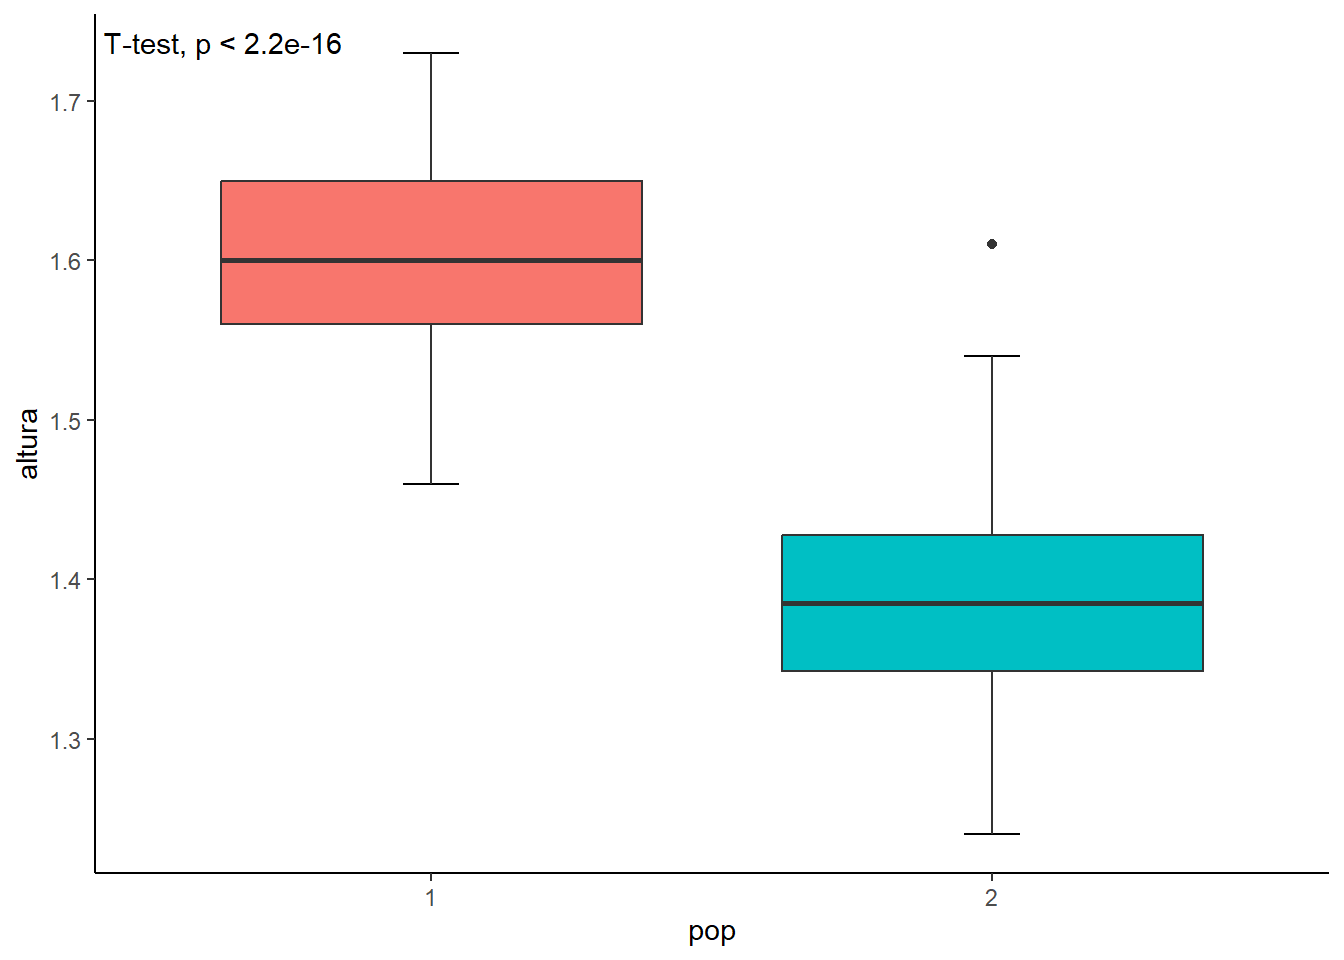
\includegraphics[width=0.7\linewidth,height=0.7\textheight]{bookdownproj_files/figure-latex/twopop-1} 

}

\caption{Comparação da altura de mulheres em duas populações}\label{fig:twopop}
\end{figure}

Observe na Figura \ref{fig:twopop} onde aparece o resultado do teste t (\(P = 2,2 \times 10^-16\)) e os boxplots (veja Seção \ref{sec-bxp}) em posições bem diferentes.

\textbf{Ativação de uma função criada}

Para ativar uma função previamente criada, usa-se a função nativa \texttt{source\ ()}. O argumento desta função é o caminho (no exemplo, é o diretório do autor) onde se encontra a função buscada, por exemplo, a função \texttt{imc()} criada acima:

\begin{Shaded}
\begin{Highlighting}[]
\FunctionTok{source}\NormalTok{(}\StringTok{\textquotesingle{}C:/Users/petro/Dropbox/Estatistica/Bioestatistica\_usando\_R/Funcoes/imc.R\textquotesingle{}}\NormalTok{)}
\end{Highlighting}
\end{Shaded}

\section{Classes}\label{classes}

São os atributos de um objeto e o seu conhecimento é de suma importância. A partir do conhecimento do tipo de classe que as funções sabem o que extamente fazer com um objeto. Por exemplo, não é possivel somar duas letras e se for feita a tentativa de somar ``a'' e ``b'', O\emph{R}retorna um erro: { Error in ``a'' + ``b'': non-numeric argument to binary operator }.

No R, os textos são escritos entre aspas simples ou duplas. As aspas servem para diferenciar nomes (objetos, funções, pacotes) de textos (letras e palavras). Os textos são muito comuns em variáveis categóricas e são popularmente chamados de \emph{strings} ou \emph{character}. Alé desta classe, o \emph{R} tem outras classes básicas que são a \emph{numeric} e a \emph{logical}. Um objeto de qualquer uma dessas classes é chamado de \emph{objeto atômico}. Esse nome se deve ao fato de essas classes não se misturarem \citep{cursor2015livro}.

Para saber qual o tipo de classe que um objeto pertence, basta usar a função \texttt{class\ ()}.

\begin{Shaded}
\begin{Highlighting}[]
\NormalTok{idade }\OtherTok{\textless{}{-}} \FunctionTok{c}\NormalTok{(}\DecValTok{3}\NormalTok{, }\DecValTok{5}\NormalTok{, }\DecValTok{7}\NormalTok{, }\DecValTok{9}\NormalTok{, }\DecValTok{6}\NormalTok{, }\DecValTok{7}\NormalTok{)}
\FunctionTok{class}\NormalTok{ (idade)}
\end{Highlighting}
\end{Shaded}

\begin{verbatim}
## [1] "numeric"
\end{verbatim}

\begin{Shaded}
\begin{Highlighting}[]
\NormalTok{nome }\OtherTok{\textless{}{-}} \FunctionTok{c}\NormalTok{(}\StringTok{"Pedro"}\NormalTok{, }\StringTok{"Maria"}\NormalTok{, }\StringTok{"Margarida"}\NormalTok{, }\StringTok{"Alice"}\NormalTok{, }\StringTok{"João"}\NormalTok{, }\StringTok{"Luís"}\NormalTok{)}
\FunctionTok{class}\NormalTok{(nome)}
\end{Highlighting}
\end{Shaded}

\begin{verbatim}
## [1] "character"
\end{verbatim}

\section{Vetores}\label{sec-vetores}

Um \textbf{vetor} é uma variável com um ou mais valores do mesmo tipo. Por exemplo, o número de filhos em 10 famílias foi
4, 5, 3, 2, 2, 1, 2, 1, 3 e 2. O vetor nomeado de \texttt{n.filhos} é um objeto numérico de comprimento = 10. A maneira mais fácil de criar um vetor em \emph{R} é concatenar (ligar) os 10 valores, usando a função concatenar \texttt{c()} assim:

\begin{Shaded}
\begin{Highlighting}[]
\NormalTok{n.filhos }\OtherTok{\textless{}{-}} \FunctionTok{c}\NormalTok{(}\DecValTok{4}\NormalTok{, }\DecValTok{5}\NormalTok{, }\DecValTok{3}\NormalTok{, }\DecValTok{2}\NormalTok{, }\DecValTok{2}\NormalTok{, }\DecValTok{1}\NormalTok{, }\DecValTok{2}\NormalTok{, }\DecValTok{1}\NormalTok{, }\DecValTok{3}\NormalTok{, }\DecValTok{2}\NormalTok{)}
\NormalTok{n.filhos}
\end{Highlighting}
\end{Shaded}

\begin{verbatim}
##  [1] 4 5 3 2 2 1 2 1 3 2
\end{verbatim}

Como os vetores são conjuntos \emph{indexados}, pode-se dizer que cada valor dentro de um vetor tem uma \textbf{posição}. Essa posição é dada pela ordem em que os elementos foram colocados no momento em que o vetor foi criado. Isso nos permite acessar individualmente cada valor de um vetor \citep{cursor2015livro}.\\
Para acessar um determinado valor, basta colocar a posição do mesmo entre colchetes {[} {]}. Se há interesse em conhecer o número de filhos da quinta família, procede-se da seguinte forma:

\begin{Shaded}
\begin{Highlighting}[]
\NormalTok{n.filhos[}\DecValTok{5}\NormalTok{]}
\end{Highlighting}
\end{Shaded}

\begin{verbatim}
## [1] 2
\end{verbatim}

Se houver tentativa de acessar um valor inexixtente, o \emph{R} retorna \texttt{NA}.

\begin{Shaded}
\begin{Highlighting}[]
\NormalTok{n.filhos[}\DecValTok{11}\NormalTok{]}
\end{Highlighting}
\end{Shaded}

\begin{verbatim}
## [1] NA
\end{verbatim}

Se houver necessidade de excluir um dos elementos, basta colocar entre colchetes a posição do mesmo com sinal negativo. Por exemplo, para excluir o valor correspondente a sexta família, usa-se:

\begin{Shaded}
\begin{Highlighting}[]
\NormalTok{n.filhos[}\SpecialCharTok{{-}}\DecValTok{6}\NormalTok{]}
\end{Highlighting}
\end{Shaded}

\begin{verbatim}
## [1] 4 5 3 2 2 2 1 3 2
\end{verbatim}

Observa-se que o valor 1 foi excluído da série de elementos.

Quando são colocados elementos em um vetor que pertençam a classes diferentes, o \emph{R} promove o que se denomina de \textbf{coerção}, pois o vetor pode ter apenas uma classe de objeto. Dessa forma, as classes mais fortes reprimem as mais fracas. Por exemplo, sempre que for misturado números e texto em um vetor, os números serão considerados como texto:

\begin{Shaded}
\begin{Highlighting}[]
\NormalTok{vetor }\OtherTok{\textless{}{-}} \FunctionTok{c}\NormalTok{(}\DecValTok{12}\NormalTok{, }\DecValTok{15}\NormalTok{, }\DecValTok{4}\NormalTok{, }\DecValTok{6}\NormalTok{, }\StringTok{"A"}\NormalTok{, }\StringTok{"D"}\NormalTok{)}
\NormalTok{vetor}
\end{Highlighting}
\end{Shaded}

\begin{verbatim}
## [1] "12" "15" "4"  "6"  "A"  "D"
\end{verbatim}

Observe que, agora, todos os elementos do vetor passaram a ser textos e, porisso, estão entre aspas.

\subsection{Tipos de vetores}\label{tipos-de-vetores}

Dado um vetor, pode-se determinar seu tipo com \texttt{typeof()}, ou verificar se é um tipo específico com uma das funções: \texttt{is.character()}, 'is.double()\texttt{,}is.integer()\texttt{,}is.logical( )`.

\begin{Shaded}
\begin{Highlighting}[]
\NormalTok{n.filhos }\OtherTok{\textless{}{-}} \FunctionTok{c}\NormalTok{(}\DecValTok{4}\NormalTok{, }\DecValTok{5}\NormalTok{, }\DecValTok{3}\NormalTok{, }\DecValTok{2}\NormalTok{, }\DecValTok{2}\NormalTok{, }\DecValTok{1}\NormalTok{, }\DecValTok{2}\NormalTok{, }\DecValTok{1}\NormalTok{, }\DecValTok{3}\NormalTok{, }\DecValTok{2}\NormalTok{)}
\FunctionTok{typeof}\NormalTok{(n.filhos)}
\end{Highlighting}
\end{Shaded}

\begin{verbatim}
## [1] "double"
\end{verbatim}

\begin{Shaded}
\begin{Highlighting}[]
\FunctionTok{is.numeric}\NormalTok{(n.filhos)}
\end{Highlighting}
\end{Shaded}

\begin{verbatim}
## [1] TRUE
\end{verbatim}

As expressões do tipo \emph{character} devem aparecer entre aspas duplas ou simples. Os números no \emph{R} são geralmente tratados como objetos numéricos (números reais de dupla precisão). Mesmo números inteiros são tratados como numéricos. Para fazer um número inteiro ser tratado como objeto inteiro, deve-se utilizar a letra L após o número.

Os valores lógicos (ou booleanos) são TRUE ou FALSE. T ou F também são aceitos.

\begin{Shaded}
\begin{Highlighting}[]
\NormalTok{n.filhos }\OtherTok{\textless{}{-}} \FunctionTok{c}\NormalTok{(}\DecValTok{4}\DataTypeTok{L}\NormalTok{, }\DecValTok{5}\DataTypeTok{L}\NormalTok{, }\DecValTok{3}\DataTypeTok{L}\NormalTok{, }\DecValTok{2}\DataTypeTok{L}\NormalTok{, }\DecValTok{2}\DataTypeTok{L}\NormalTok{, }\DecValTok{1}\DataTypeTok{L}\NormalTok{, }\DecValTok{2}\DataTypeTok{L}\NormalTok{, }\DecValTok{1}\DataTypeTok{L}\NormalTok{, }\DecValTok{3}\DataTypeTok{L}\NormalTok{, }\DecValTok{2}\DataTypeTok{L}\NormalTok{)}
\FunctionTok{typeof}\NormalTok{(n.filhos)}
\end{Highlighting}
\end{Shaded}

\begin{verbatim}
## [1] "integer"
\end{verbatim}

\begin{Shaded}
\begin{Highlighting}[]
\FunctionTok{is.numeric}\NormalTok{(n.filhos)}
\end{Highlighting}
\end{Shaded}

\begin{verbatim}
## [1] TRUE
\end{verbatim}

\begin{Shaded}
\begin{Highlighting}[]
\FunctionTok{is.double}\NormalTok{(n.filhos)}
\end{Highlighting}
\end{Shaded}

\begin{verbatim}
## [1] FALSE
\end{verbatim}

\begin{Shaded}
\begin{Highlighting}[]
\NormalTok{nomes }\OtherTok{\textless{}{-}} \FunctionTok{c}\NormalTok{(}\StringTok{\textquotesingle{}Maria\textquotesingle{}}\NormalTok{, }\StringTok{\textquotesingle{}João\textquotesingle{}}\NormalTok{, }\StringTok{\textquotesingle{}Manuel\textquotesingle{}}\NormalTok{, }\StringTok{\textquotesingle{}Petronio\textquotesingle{}}\NormalTok{, }\StringTok{\textquotesingle{}José\textquotesingle{}}\NormalTok{)}
\FunctionTok{typeof}\NormalTok{(nomes)}
\end{Highlighting}
\end{Shaded}

\begin{verbatim}
## [1] "character"
\end{verbatim}

\begin{Shaded}
\begin{Highlighting}[]
\FunctionTok{is.numeric}\NormalTok{(nomes)}
\end{Highlighting}
\end{Shaded}

\begin{verbatim}
## [1] FALSE
\end{verbatim}

\begin{Shaded}
\begin{Highlighting}[]
\FunctionTok{is.double}\NormalTok{(nomes)}
\end{Highlighting}
\end{Shaded}

\begin{verbatim}
## [1] FALSE
\end{verbatim}

\begin{Shaded}
\begin{Highlighting}[]
\NormalTok{altura }\OtherTok{\textless{}{-}} \FunctionTok{c}\NormalTok{(}\FloatTok{1.60}\NormalTok{, }\FloatTok{1.78}\NormalTok{, }\FloatTok{1.55}\NormalTok{, }\FloatTok{1.67}\NormalTok{, }\FloatTok{1.69}\NormalTok{)}
\FunctionTok{typeof}\NormalTok{(altura)}
\end{Highlighting}
\end{Shaded}

\begin{verbatim}
## [1] "double"
\end{verbatim}

\begin{Shaded}
\begin{Highlighting}[]
\FunctionTok{is.numeric}\NormalTok{(altura)}
\end{Highlighting}
\end{Shaded}

\begin{verbatim}
## [1] TRUE
\end{verbatim}

\begin{Shaded}
\begin{Highlighting}[]
\FunctionTok{is.double}\NormalTok{(altura)}
\end{Highlighting}
\end{Shaded}

\begin{verbatim}
## [1] TRUE
\end{verbatim}

\section{Dataframes}\label{sec-dataframes}

\textbf{Dataframes} são objetos de dados genéricos de R, usados para armazenar os dados tabulares, onde os dados são organizados de maneira lógica em um formato de linha-e-coluna semelhante ao de uma planilha do Excel. O data frame é uma estrutura bidimensional. Estas dimensões podem ser encontradas com a função \texttt{dim()}.
Os Data frames podem ser formados com objetos criados previamente, desde que tenham o mesmo comprimento \citep{zuur2009beginner}.

Abaixo serão criadas algumas variáveis, todas relacionadas ao nascimento de 15 bebês:

\begin{Shaded}
\begin{Highlighting}[]
\NormalTok{id }\OtherTok{\textless{}{-}} \FunctionTok{c}\NormalTok{(}\DecValTok{1}\NormalTok{, }\DecValTok{2}\NormalTok{, }\DecValTok{3}\NormalTok{, }\DecValTok{4}\NormalTok{, }\DecValTok{5}\NormalTok{, }\DecValTok{6}\NormalTok{, }\DecValTok{7}\NormalTok{, }\DecValTok{8}\NormalTok{, }\DecValTok{9}\NormalTok{, }\DecValTok{10}\NormalTok{, }\DecValTok{11}\NormalTok{, }\DecValTok{12}\NormalTok{, }\DecValTok{13}\NormalTok{, }\DecValTok{14}\NormalTok{, }\DecValTok{15}\NormalTok{)}
\NormalTok{pesoRN }\OtherTok{\textless{}{-}} \FunctionTok{c}\NormalTok{ (}\DecValTok{3340}\NormalTok{,}\DecValTok{3345}\NormalTok{,}\DecValTok{3750}\NormalTok{,}\DecValTok{3650}\NormalTok{,}\DecValTok{3220}\NormalTok{,}\DecValTok{4070}\NormalTok{,}\DecValTok{3380}\NormalTok{,}\DecValTok{3970}\NormalTok{,}\DecValTok{3060}\NormalTok{,}\DecValTok{3180}\NormalTok{,  }
             \DecValTok{2865}\NormalTok{,}\DecValTok{2815}\NormalTok{,}\DecValTok{3245}\NormalTok{,}\DecValTok{2051}\NormalTok{,}\DecValTok{2630}\NormalTok{)  }
\NormalTok{compRN }\OtherTok{\textless{}{-}} \FunctionTok{c}\NormalTok{ (}\DecValTok{50}\NormalTok{,}\DecValTok{48}\NormalTok{,}\DecValTok{52}\NormalTok{,}\DecValTok{48}\NormalTok{,}\DecValTok{50}\NormalTok{,}\DecValTok{51}\NormalTok{,}\DecValTok{50}\NormalTok{,}\DecValTok{51}\NormalTok{,}\DecValTok{47}\NormalTok{,}\DecValTok{47}\NormalTok{,}\DecValTok{47}\NormalTok{,}\DecValTok{49}\NormalTok{,}\DecValTok{51}\NormalTok{,}\DecValTok{50}\NormalTok{,}\DecValTok{44}\NormalTok{)}
\NormalTok{sexo }\OtherTok{\textless{}{-}} \FunctionTok{c}\NormalTok{ (}\DecValTok{2}\NormalTok{,}\DecValTok{2}\NormalTok{,}\DecValTok{2}\NormalTok{,}\DecValTok{1}\NormalTok{,}\DecValTok{1}\NormalTok{,}\DecValTok{1}\NormalTok{,}\DecValTok{2}\NormalTok{,}\DecValTok{1}\NormalTok{,}\DecValTok{1}\NormalTok{,}\DecValTok{1}\NormalTok{,}\DecValTok{2}\NormalTok{,}\DecValTok{2}\NormalTok{,}\DecValTok{1}\NormalTok{,}\DecValTok{1}\NormalTok{,}\DecValTok{2}\NormalTok{)}
\NormalTok{tipoParto }\OtherTok{\textless{}{-}} \FunctionTok{c}\NormalTok{ (}\DecValTok{1}\NormalTok{,}\DecValTok{1}\NormalTok{,}\DecValTok{2}\NormalTok{,}\DecValTok{1}\NormalTok{,}\DecValTok{2}\NormalTok{,}\DecValTok{2}\NormalTok{,}\DecValTok{1}\NormalTok{,}\DecValTok{2}\NormalTok{,}\DecValTok{1}\NormalTok{,}\DecValTok{1}\NormalTok{,}\DecValTok{1}\NormalTok{,}\DecValTok{2}\NormalTok{,}\DecValTok{1}\NormalTok{,}\DecValTok{1}\NormalTok{,}\DecValTok{1}\NormalTok{)}
\NormalTok{idadeMae }\OtherTok{\textless{}{-}} \FunctionTok{c}\NormalTok{ (}\DecValTok{40}\NormalTok{,}\DecValTok{19}\NormalTok{,}\DecValTok{26}\NormalTok{,}\DecValTok{19}\NormalTok{,}\DecValTok{32}\NormalTok{,}\DecValTok{24}\NormalTok{,}\DecValTok{27}\NormalTok{,}\DecValTok{20}\NormalTok{,}\DecValTok{21}\NormalTok{,}\DecValTok{19}\NormalTok{,}\DecValTok{23}\NormalTok{,}\DecValTok{36}\NormalTok{,}\DecValTok{21}\NormalTok{,}\DecValTok{23}\NormalTok{,}\DecValTok{23}\NormalTok{) }
\end{Highlighting}
\end{Shaded}

Tem-se um grupo de variáveis isoladas. Seria útil reuni-las em um só objeto, usando a função \texttt{data.frame()}. Este novo objeto receberá o nome de \texttt{dadosNeonatos}.

\begin{Shaded}
\begin{Highlighting}[]
\NormalTok{dadosNeonatos }\OtherTok{\textless{}{-}} \FunctionTok{data.frame}\NormalTok{ (id,}
\NormalTok{                             pesoRN, }
\NormalTok{                             compRN, }
\NormalTok{                             sexo, }
\NormalTok{                             tipoParto, }
\NormalTok{                             idadeMae)}
\end{Highlighting}
\end{Shaded}

Ao ser executado o comando retornará um novo objeto da classe \texttt{data.frame}:

\begin{Shaded}
\begin{Highlighting}[]
\FunctionTok{class}\NormalTok{ (dadosNeonatos)}
\end{Highlighting}
\end{Shaded}

\begin{verbatim}
## [1] "data.frame"
\end{verbatim}

Havendo necessidade de acrescentar outra variável no banco de dados \texttt{dadosNeonatos}, por exemplo, os dados da ida ou não dos recém-nascidos para a UTI. Para isso, será atribuido a um vetor, contendo a situação dos 15 recém-nascidos, o nome de utiNeo e para relacioná-lo a uma coluna do dataframe dadosNeonatos, será usado o símbolo \$, como mostrado abaixo \footnote{A variável criada, \texttt{utiNeo}, possui dois níveis: 1 = sim; 2 = não, referente se o bebê foi ou não para a UTI.}:

\begin{Shaded}
\begin{Highlighting}[]
\NormalTok{dadosNeonatos}\SpecialCharTok{$}\NormalTok{utiNeo }\OtherTok{\textless{}{-}} \FunctionTok{c}\NormalTok{ (}\DecValTok{2}\NormalTok{,}\DecValTok{2}\NormalTok{,}\DecValTok{2}\NormalTok{,}\DecValTok{2}\NormalTok{,}\DecValTok{1}\NormalTok{,}\DecValTok{2}\NormalTok{,}\DecValTok{1}\NormalTok{,}\DecValTok{2}\NormalTok{,}\DecValTok{2}\NormalTok{,}\DecValTok{2}\NormalTok{,}\DecValTok{2}\NormalTok{,}\DecValTok{1}\NormalTok{,}\DecValTok{2}\NormalTok{,}\DecValTok{2}\NormalTok{,}\DecValTok{2}\NormalTok{)}
\end{Highlighting}
\end{Shaded}

Para observar o novo banco de dados, pode-se usar a função \texttt{str()} do \emph{R} base. Digitar no \emph{R Script}:

\begin{Shaded}
\begin{Highlighting}[]
\FunctionTok{str}\NormalTok{ (dadosNeonatos)}
\end{Highlighting}
\end{Shaded}

\begin{verbatim}
## 'data.frame':    15 obs. of  7 variables:
##  $ id       : num  1 2 3 4 5 6 7 8 9 10 ...
##  $ pesoRN   : num  3340 3345 3750 3650 3220 ...
##  $ compRN   : num  50 48 52 48 50 51 50 51 47 47 ...
##  $ sexo     : num  2 2 2 1 1 1 2 1 1 1 ...
##  $ tipoParto: num  1 1 2 1 2 2 1 2 1 1 ...
##  $ idadeMae : num  40 19 26 19 32 24 27 20 21 19 ...
##  $ utiNeo   : num  2 2 2 2 1 2 1 2 2 2 ...
\end{verbatim}

Observando a saida da função, verifica-se que o dataframe contém 15 linhas e 6 colunas e que todas as variáveis estão como variáveis \emph{numéricas} , mas as variáveis \texttt{sexo}, \texttt{tipoParto} são variáveis \emph{categóricas}, bem como a variável \texttt{utiNeo}, acrescentada depois. Há necessidade de fazer uma transformação dessas variáveis.

\section{Fatores}\label{sec-fatores}

Os fatores, no R, são usados para trabalhar com variáveis categóricas. São variáveis usadas para categorizar e armazenar os dados, tendo um número limitado de valores diferentes.

Um fator armazena os dados como um vetor de valores inteiros. O fator em \emph{R} também é conhecido como uma variável categórica que armazena valores de dados de \emph{string} e inteiros como níveis. O fator é usado principalmente em modelagem estatística e análise exploratória de dados com \emph{R} \citep{wickham2017factors}.

\subsection{Criando fatores}\label{criando-fatores}

No data frame dadosNeonatos, criado anteriormente, contém três variáveis (\texttt{sexo}, \texttt{tipoParto} e \texttt{utiNeo}) que estão como variáveis numéricas. É possível, desta forma, realizar operações aritméticas com elas. Isto, obviamente, seria um absurdo. Assim, é necessário transformá-las em fatores. Para isso, é usada a função \texttt{factor()}, nativa do \emph{R}. Os principais argumentos desta função são:

\begin{itemize}
\tightlist
\item
  \textbf{x} \(\longrightarrow\) vetor numérico
\item
  \textbf{levels} \(\longrightarrow\) vetor opcional dos valores que \emph{x} pode assumir
\item
  \textbf{labels} \(\longrightarrow\) vetor de caracteres dos rótulos para os níveis, na mesma ordem
\item
  \textbf{ordered} \(\longrightarrow\) vetor lógico (TRUE ou FALSE). Se TRUE, os níveis dos fatores são assumidos como ordenados
\end{itemize}

No exemplo, as variáveis não têm uma ordem lógica, então, o argumento \texttt{ordered} não será usado.

\begin{Shaded}
\begin{Highlighting}[]
\NormalTok{dadosNeonatos}\SpecialCharTok{$}\NormalTok{utiNeo }\OtherTok{\textless{}{-}} \FunctionTok{factor}\NormalTok{ (dadosNeonatos}\SpecialCharTok{$}\NormalTok{utiNeo,}
                                \AttributeTok{levels =} \FunctionTok{c}\NormalTok{(}\DecValTok{1}\NormalTok{,}\DecValTok{2}\NormalTok{), }
                                \AttributeTok{labels =} \FunctionTok{c}\NormalTok{(}\StringTok{\textquotesingle{}sim\textquotesingle{}}\NormalTok{,}\StringTok{\textquotesingle{}não\textquotesingle{}}\NormalTok{))}
\NormalTok{dadosNeonatos}\SpecialCharTok{$}\NormalTok{tipoParto }\OtherTok{\textless{}{-}} \FunctionTok{factor}\NormalTok{(dadosNeonatos}\SpecialCharTok{$}\NormalTok{tipoParto, }
                                   \AttributeTok{levels =} \FunctionTok{c}\NormalTok{(}\DecValTok{1}\NormalTok{,}\DecValTok{2}\NormalTok{),}
                                   \AttributeTok{labels =} \FunctionTok{c}\NormalTok{(}\StringTok{"normal"}\NormalTok{,}\StringTok{"cesareo"}\NormalTok{))}
\NormalTok{dadosNeonatos}\SpecialCharTok{$}\NormalTok{sexo }\OtherTok{\textless{}{-}} \FunctionTok{factor}\NormalTok{ (dadosNeonatos}\SpecialCharTok{$}\NormalTok{sexo, }
                               \AttributeTok{levels =} \FunctionTok{c}\NormalTok{(}\DecValTok{1}\NormalTok{,}\DecValTok{2}\NormalTok{), }
                               \AttributeTok{labels =} \FunctionTok{c}\NormalTok{(}\StringTok{"M"}\NormalTok{,}\StringTok{"F"}\NormalTok{)) }
\end{Highlighting}
\end{Shaded}

Após a transformação, executa-se novamente a função \texttt{str()} para ver como ficou o dataframe:

\begin{Shaded}
\begin{Highlighting}[]
\FunctionTok{str}\NormalTok{(dadosNeonatos)}
\end{Highlighting}
\end{Shaded}

\begin{verbatim}
## 'data.frame':    15 obs. of  7 variables:
##  $ id       : num  1 2 3 4 5 6 7 8 9 10 ...
##  $ pesoRN   : num  3340 3345 3750 3650 3220 ...
##  $ compRN   : num  50 48 52 48 50 51 50 51 47 47 ...
##  $ sexo     : Factor w/ 2 levels "M","F": 2 2 2 1 1 1 2 1 1 1 ...
##  $ tipoParto: Factor w/ 2 levels "normal","cesareo": 1 1 2 1 2 2 1 2 1 1 ...
##  $ idadeMae : num  40 19 26 19 32 24 27 20 21 19 ...
##  $ utiNeo   : Factor w/ 2 levels "sim","não": 2 2 2 2 1 2 1 2 2 2 ...
\end{verbatim}

Agora, as três varáveis passaram a ser fatores e as outras mantiveram-se numéricas.

Desta forma, é possível trabalhar com ela fazendo, por exemplo, uma contagem da frequência do tipo de parto, usando a função \texttt{table()}:

\begin{Shaded}
\begin{Highlighting}[]
\FunctionTok{table}\NormalTok{(dadosNeonatos}\SpecialCharTok{$}\NormalTok{tipoParto)}
\end{Highlighting}
\end{Shaded}

\begin{verbatim}
## 
##  normal cesareo 
##      10       5
\end{verbatim}

Ou seja, aproximadamente 70\% dos partos desta amostra são normais.

\subsection{Salvando o dataframe criado}\label{salvando-o-dataframe-criado}

O data frame, criado e modificado anteriormente, pode ser salvo para uso posterior no diretório de trabalho.

Para isso existe a função \texttt{save\ ()}, fornecendo como argumentos o data frame a ser salvo e o nome do arquivo (\texttt{file\ =}) entre aspas. Por convenção, esta função salva com a extensão \texttt{.RData} que deve ser digitada, pois o \emph{R} não a adiciona automaticamente.

\begin{Shaded}
\begin{Highlighting}[]
\FunctionTok{save}\NormalTok{(dadosNeonatos, }\AttributeTok{file =} \StringTok{"dadosNeonatos.RData"}\NormalTok{)}
\end{Highlighting}
\end{Shaded}

Este comando colocará o arquivo no diretório de trabalho em uso. Portanto, se o objetivo é salvar em outro local, deve ser informado ao \emph{R} qual o novo diretório.

Para carregar o objeto salvo anteriormente com o comando \texttt{save\ ()}, usa-se a função \texttt{load\ ()}. Se o arquivo a ser lido não estiver no diretório de trabalho da sessão, há necessidade de especificar o caminho até o arquivo:

\begin{Shaded}
\begin{Highlighting}[]
\FunctionTok{load}\NormalTok{(}\StringTok{"dadosNeonatos.RData"}\NormalTok{)}
\end{Highlighting}
\end{Shaded}

Ou, indicando o diretório onde está o arquivo:

\begin{Shaded}
\begin{Highlighting}[]
\FunctionTok{load}\NormalTok{(}\StringTok{"C:/Users/petro/Dropbox/Estatistica/Meus\_Livros/Bioestatistica\_R/Book/dadosNeonatos.RData"}\NormalTok{)}
\end{Highlighting}
\end{Shaded}

É possível salvar em outro tipo de extensão como Excel (\texttt{.xlsx}), Valores Separados por Vírgula (\texttt{.csv}), etc. O procedimento é o mesmo, mudando a função. Para salvar em uma extensão \texttt{.xlsx},utiliza-se a função \texttt{write\_xlsx\ ()} do pacote \texttt{writexl} \citep{ooms2022writexl}:

\begin{Shaded}
\begin{Highlighting}[]
\NormalTok{writexl}\SpecialCharTok{::}\FunctionTok{write\_xlsx}\NormalTok{(dadosNeonatos, }\StringTok{"dadosNeonatos.xlsx"}\NormalTok{)}
\end{Highlighting}
\end{Shaded}

Para salvar com a extensão \texttt{.csv}, usar a função \texttt{write.csv()} ou \texttt{write.csv2()} que faz parte do pacote \texttt{utils}, incluido no \emph{R} base. A primeira função, usa \texttt{"."} para a separação dos decimais e \texttt{","} para separar as variáveis; a segunda função usa \texttt{","} para os decimais e \texttt{";"} para separar as variáveis, convenção do Excel para algumas localidades, como o Brasil \citep{write2022csv}. Portanto, uma maneira de salvar o arquivo é:

\begin{Shaded}
\begin{Highlighting}[]
\FunctionTok{write.csv2}\NormalTok{ (dadosNeonatos, }\StringTok{"dadosNeonatos.csv"}\NormalTok{)}
\end{Highlighting}
\end{Shaded}

\chapter{\texorpdfstring{Manipulando os dados no \emph{R Studio}}{Manipulando os dados no R Studio}}\label{manipulando-os-dados-no-r-studio}

\section{\texorpdfstring{Importando dados de outros \emph{softwares}}{Importando dados de outros softwares}}\label{importando-dados-de-outros-softwares}

Foi visto. quando estudou-se os dataframes, que é possível inserir dados diretamente no \emph{R}. Entretanto, se o conjunto de dados for muito extenso, torna-se complicado. Desta forma, é melhor importar os dados de outro software, como o Excel, SPSS, etc. A recomendação é que se construa o banco de dados, por exemplo, no Excel, e, depois, exporte o arquivo em um formato que o\emph{R}reconheça -- \texttt{.xlsx}, \texttt{.csv}, \texttt{.sav}.

\subsection{Importando dados de um arquivo CSV}\label{sec-csv}

O formato CSV significa \emph{Comma Separated Values}, ou seja, é um arquivo de valores separados por vírgula. Esse formato de armazenamento é simples e agrupa informações de arquivos de texto em planilhas. É possível gerar um arquivo \texttt{.csv}, a partir de uma planilha do Excel, usando o menu \texttt{salvar\ como} e escolher \texttt{CSV}.

As funções \texttt{read.csv()} e \texttt{read.csv2()}, incluídas no\emph{R}base, podem ser utilizadas para importar arquivos CSV. Existe uma pequena diferença entre elas. Dois argumentos dessas funções têm padrão diferentes em cada uma. São eles: \texttt{sep} (separador de colunas) e \texttt{dec} (separador de decimais). Em \texttt{read.csv()}, o padrão é \texttt{sep\ =\ ”,”} e \texttt{dec\ =\ ”.”} e em \texttt{read.csv2()} o padrão é \texttt{sep\ =\ “;”} e \texttt{dec\ =\ ”,”}. Portanto, quando se importa um arquivo \texttt{.csv}, é importante saber qual a sua estrutura. Verificar se os decimais estão separados por \emph{ponto} ou por \emph{vírgula} e se as colunas (variáveis), por \emph{vírgula} ou \emph{ponto e vírgula}. Para ver isso, basta abrir o arquivo em um bloco de notas (por exemplo, \emph{Bloco de Notas do Windows}, \emph{Notepad ++}).

Quando se usa o \texttt{read.csv()} há necessidade de informar o separador e o decimal, pois senão ele usará o padrão inglês e o arquivo não será lido. Já com \texttt{read.csv2()}, que usa o padrão brasileiro, não há necessidade de informar ao\emph{R}qual o separador de colunas e nem o separador dos decimais.

Além disso, é necessário saber em que diretório do computador está o arquivo para informar ao comando. Recomenda-se colocar o arquivo na pasta do diretório de trabalho, pois assim basta apenas colocar o nome do arquivo na função de leitura dos dados. Caso contrário, tem-se que se usar todo o caminho (\emph{path}).

Como exemplo, será importado o arquivo \texttt{dadosNeonatos.csv} que se encontra no diretório de trabalho do autor, salvo anteriormente. Para obter o arquivo, clique no \href{https://github.com/petronioliveira/Arquivos/blob/main/dadosNeonatos.csv}{\textbf{link}} e salve em seu diretório de trabalho.

A estrutura deste arquivo mostra que as colunas estão separadas por ponto-e-virgula e, portanto, a leitura dos dados será feita com a função \texttt{read.csv2()} e, como o arquivo está no diretório de trabalho, não há necessidade de informar o diretório completo. Os dados serão colocados em um objeto de nome \texttt{neonatos} \footnote{A mudança do nome do dataframe de dadosNeonatos para neonatos é desnecessária. Foi realizada apenas por questões didáticas.}:

\begin{Shaded}
\begin{Highlighting}[]
\NormalTok{neonatos }\OtherTok{\textless{}{-}} \FunctionTok{read.csv2}\NormalTok{(}\StringTok{"./Arquivos/dadosNeonatos.csv"}\NormalTok{)}
\end{Highlighting}
\end{Shaded}

Use a função \texttt{str()} para visualizar o conjunto de dados:\footnote{Observe, na saída, que na variável \texttt{utiNeo} aparece palavras com acentuação (``não''). Às vezes, ao abrir o arquivo com a função \texttt{read.csv2()}, pode acontecer de esta palavra aparecer, por exemplo, como: ``n\xe3o''. Louco, não é? Se ocorrer isso, use, após o nome do arquivo e separado por vírgula, o argumento \texttt{fileEncoding\ =\ “latin1”}. Dessa forma, o erro será corrigido.}

\begin{Shaded}
\begin{Highlighting}[]
\FunctionTok{str}\NormalTok{(neonatos)}
\end{Highlighting}
\end{Shaded}

\begin{verbatim}
## 'data.frame':    15 obs. of  7 variables:
##  $ id       : int  1 2 3 4 5 6 7 8 9 10 ...
##  $ pesoRN   : int  3340 3345 3750 3650 3220 4070 3380 3970 3060 3180 ...
##  $ compRN   : int  50 48 52 48 50 51 50 51 47 47 ...
##  $ sexo     : chr  "F" "F" "F" "M" ...
##  $ tipoParto: chr  "normal" "normal" "cesareo" "normal" ...
##  $ idadeMae : int  40 19 26 19 32 24 27 20 21 19 ...
##  $ utiNeo   : chr  "não" "não" "não" "não" ...
\end{verbatim}

Recentemente, foi desenvolvido o pacote \texttt{readr}, incluído no conjunto de pacotes \texttt{tidyverse}\citet{wickham2019tidyverse}, para lidar rapidamente com a leitura de grandes arquivos. O pacote fornece substituições para funções como \texttt{read.csv()}. As funções \texttt{read\_csv()} e \texttt{read\_csv2()} oferecidas pelo \texttt{readr} são análogas às do\emph{R}base. Entretanto, são muito mais rápidas e fornecem mais recursos, como um método compacto para especificar tipos de coluna. Além disso, produzem \texttt{tibbles} (ver adiante, neste mesmo capítulo) que são mais reproduzíveis, pois as funções básicas do R herdam alguns comportamentos do sistema operacional e das variáveis de ambiente, portanto, o código de importação que funciona no seu computador pode não funcionar no de outra pessoa.
Para usar a função é necessário instalar e ativar o pacote \texttt{readr}. A função \texttt{read\_csv2()} será utilizada para criar um outro objeto de nome \texttt{recemNascidos}, mas o conjunto de dados a ser ativado é o mesmo (\texttt{dadosNeonatos}):

\begin{Shaded}
\begin{Highlighting}[]
 \FunctionTok{library}\NormalTok{(readr)}
\NormalTok{ recemNascidos }\OtherTok{\textless{}{-}} \FunctionTok{read\_csv2}\NormalTok{(}\StringTok{"Arquivos/dadosNeonatos.csv"}\NormalTok{)}
\end{Highlighting}
\end{Shaded}

\begin{verbatim}
## i Using "','" as decimal and "'.'" as grouping mark. Use `read_delim()` for more control.
\end{verbatim}

\begin{verbatim}
## Rows: 15 Columns: 7
## -- Column specification --------------------------------------------------------
## Delimiter: ";"
## chr (3): sexo, tipoParto, utiNeo
## dbl (4): id, pesoRN, compRN, idadeMae
## 
## i Use `spec()` to retrieve the full column specification for this data.
## i Specify the column types or set `show_col_types = FALSE` to quiet this message.
\end{verbatim}

Quando você executa \texttt{read\_csv2()}, ele imprime uma especificação de coluna que fornece o nome e o tipo de cada coluna.

Novamente, a função \texttt{str()} mostrará a estrutura do arquivo \footnote{Da mesma maneira, como acontece com a função \texttt{read.csv2()}, a função equivalente do \texttt{readr} pode retornar erro na leitura de palavras com acento. Para corrigir isso, usa-se o argumento \texttt{locale\ (encoding\ =\ "latin1")}}:

\begin{Shaded}
\begin{Highlighting}[]
\FunctionTok{str}\NormalTok{(recemNascidos)}
\end{Highlighting}
\end{Shaded}

\begin{verbatim}
## spc_tbl_ [15 x 7] (S3: spec_tbl_df/tbl_df/tbl/data.frame)
##  $ id       : num [1:15] 1 2 3 4 5 6 7 8 9 10 ...
##  $ pesoRN   : num [1:15] 3340 3345 3750 3650 3220 ...
##  $ compRN   : num [1:15] 50 48 52 48 50 51 50 51 47 47 ...
##  $ sexo     : chr [1:15] "F" "F" "F" "M" ...
##  $ tipoParto: chr [1:15] "normal" "normal" "cesareo" "normal" ...
##  $ idadeMae : num [1:15] 40 19 26 19 32 24 27 20 21 19 ...
##  $ utiNeo   : chr [1:15] "não" "não" "não" "não" ...
##  - attr(*, "spec")=
##   .. cols(
##   ..   id = col_double(),
##   ..   pesoRN = col_double(),
##   ..   compRN = col_double(),
##   ..   sexo = col_character(),
##   ..   tipoParto = col_character(),
##   ..   idadeMae = col_double(),
##   ..   utiNeo = col_character()
##   .. )
##  - attr(*, "problems")=<externalptr>
\end{verbatim}

\subsection{Importando um arquivo do Excel}\label{sec-xlsx}

O pacote \texttt{readxl}, pertencente ao conjunto de pacotes do \texttt{tidyverse}, facilita a obtenção de dados do Excel para o R, através da função \texttt{read\_excel()}. esta função tem o argumento \texttt{sheet\ =} , que deve ser usado indicando o número ou o nome da planilha, colocado entre aspas. Este argumento é importante se houver mais de uma planilha, caso contrário, ele é opcional. Para saber os outros argumentos da função, colque o cursor dentro da função e aperte a tecla \texttt{Tab} (Figura \ref{fig:sheet}). Isto abrirá um menu com os argumentos:

\begin{figure}[H]

{\centering \includegraphics[width=0.8\linewidth]{https://i.imgur.com/5qY7z0C} 

}

\caption{Argumentos da função para importar arquivos xlsx}\label{fig:sheet}
\end{figure}

Será feita a leitura dos mesmos dados, usados na leitura de dados \texttt{csv}, apenas o arquivo agora está no formato \texttt{.xlsx}. Para obter o arquivo, siga os mesmos passos, usados anteriormente. Clique no \href{https://github.com/petronioliveira/Arquivos/blob/main/dadosNeonatos.xlsx}{\textbf{link}} e salve em seu diretório de trabalho.

Os dados serão atribuídos a um objeto com outro nome (\texttt{recemNatos}):

\begin{Shaded}
\begin{Highlighting}[]
\FunctionTok{library}\NormalTok{(readxl)}
\NormalTok{recemNatos }\OtherTok{\textless{}{-}} \FunctionTok{read\_excel}\NormalTok{(}\StringTok{"Arquivos/dadosNeonatos.xlsx"}\NormalTok{)}
\FunctionTok{str}\NormalTok{(recemNatos)}
\end{Highlighting}
\end{Shaded}

\begin{verbatim}
## tibble [15 x 7] (S3: tbl_df/tbl/data.frame)
##  $ id       : num [1:15] 1 2 3 4 5 6 7 8 9 10 ...
##  $ pesoRN   : num [1:15] 3340 3345 3750 3650 3220 ...
##  $ compRN   : num [1:15] 50 48 52 48 50 51 50 51 47 47 ...
##  $ sexo     : chr [1:15] "F" "F" "F" "M" ...
##  $ tipoParto: chr [1:15] "normal" "normal" "cesareo" "normal" ...
##  $ idadeMae : num [1:15] 40 19 26 19 32 24 27 20 21 19 ...
##  $ utiNeo   : chr [1:15] "não" "não" "não" "não" ...
\end{verbatim}

Na Figura \ref{fig:sheet}, o duplo dois pontos (\texttt{::}) precedido do nome pacote, no caso \texttt{readr}, especifica a procedência da função usada. Nesta situação, não há necessidade de usar a função \texttt{library()} para carregar o pacote já instalado em um diretório (biblioteca) previamente.

\subsection{Importando arquivos com o RStudio}\label{importando-arquivos-com-o-rstudio}

O \texttt{RStudio} permite importar arquivos sem a necessidade de digitar comandos, que, para alguns podem ser tediosos.

Na tela inicial do \texttt{RStudio}, à direita, na parte superior, clique na aba \emph{Environment} e em \texttt{Import\ Dataset}. Esta ação abre um menu que permite importar arquivos .csv, Excel, SPSS, etc.

Por exemplo, para importar o arquivo \texttt{dadosNeonatos.xlsx}, clicar em \texttt{From\ Excel...} Abre uma janela com uma caixa de diálogo. Clicar no botão \texttt{Browse...}, localizado em cima à direita, para buscar o arquivo \texttt{dadosNeonatos.xlsx}. Assim que o arquivo for aberto, ele mostra uma \emph{preview} do arquivo e, em baixo, à direita mostra uma \emph{preview} do código (Figura \ref{fig:import}), igual ao digitado anteriormente, que cria um objeto denominado \texttt{dadosNeonatos}, nome do objeto escolhido pelo R, mas pode ser modificado na janela, à esquerda, \texttt{Import\ Option} em \texttt{Name}, onde pode-se digitar qualquer nome. Após encerrar as escolhas, clicar em \texttt{Import}.
É um caminho diferente para fazer o mesmo. Este é um dos fascínios do R!

\begin{figure}[H]

{\centering \includegraphics[width=1\linewidth]{https://i.imgur.com/xjEpK6A} 

}

\caption{Importando arquivos do excel com o RStudio.}\label{fig:import}
\end{figure}

\section{Tibble}\label{sec-tibble}

A maneira mais comum de armazenar dados no \emph{R} é usar \texttt{data.frames} ou \texttt{tibble}.

\emph{Tibble} é um novo tipo de dataframe. É como se fosse um dataframe mais moderno. Ele mantém muitos recursos importantes do data frame original, mas remove muitos dos recursos desatualizados.

Os \texttt{tibbles} são outro recurso incrível adicionado ao \emph{R} por Hadley Wickham, através do \texttt{tidyverse}, conjunto de pacotes que formam um conjunto básico de funções que facilitam a manipulação e representação gráfica dos dados \citet{wickham2019tidyverse}. Para saber mais sobre \texttt{tibble}, veja vignette(`tibbles').

A maioria dos pacotes do \emph{R} usa dataframes tradicionais, entretanto é possível transformá-los para \texttt{tibble}, usando a função \texttt{as\_tibble()}, incluída no pacote \texttt{tidyr} \citep{wickham2022tidyr}. O único propósito deste pacote é simplificar o processo de criação de \texttt{tidy\ data}(dados organizados).

O conceito de \emph{tidy data}, introduzido por Wickman \citet{wickham2014tidy}, se refere à estrutura dos dados organizados de maneira que cada linha é uma observação, cada coluna representa variáveis e cada entrada nas células do dataframe são os valores.

A transformação de um dataframe tradicional em um tibble, é um procedimento rescomendável, em função da maior flexibilidade destes.

Como exemplo deste procedimento, será usado o famoso conjunto de dados da flor iris \citet{fisher1936use} que fornece as medidas em centímetros das variáveis comprimento e largura da sepala e comprimento e largura da pétala, repectivamente, para 50 flores de cada uma das 3 espécies de íris (\emph{Iris setosa}, \emph{versicolor} e \emph{virginica}). Este conjunto de dados encontra-se no pacote \texttt{datasets} no \emph{R} base. Para visualizar os dados, será usado a função \texttt{str()}, também do \emph{R} base, que mostra a estrutura interna de um objeto:

\begin{Shaded}
\begin{Highlighting}[]
\FunctionTok{str}\NormalTok{(iris)}
\end{Highlighting}
\end{Shaded}

\begin{verbatim}
## 'data.frame':    150 obs. of  5 variables:
##  $ Sepal.Length: num  5.1 4.9 4.7 4.6 5 5.4 4.6 5 4.4 4.9 ...
##  $ Sepal.Width : num  3.5 3 3.2 3.1 3.6 3.9 3.4 3.4 2.9 3.1 ...
##  $ Petal.Length: num  1.4 1.4 1.3 1.5 1.4 1.7 1.4 1.5 1.4 1.5 ...
##  $ Petal.Width : num  0.2 0.2 0.2 0.2 0.2 0.4 0.3 0.2 0.2 0.1 ...
##  $ Species     : Factor w/ 3 levels "setosa","versicolor",..: 1 1 1 1 1 1 1 1 1 1 ...
\end{verbatim}

Observa-se que é um conjunto de dados da classe \texttt{data.frame}, contendo 150 observações de 5 variáveis (colunas). Fazendo a coerção para um \texttt{tibble}, tem-se:

\begin{Shaded}
\begin{Highlighting}[]
\FunctionTok{library}\NormalTok{(tidyr)}
\FunctionTok{as\_tibble}\NormalTok{(iris)}
\end{Highlighting}
\end{Shaded}

\begin{verbatim}
## # A tibble: 150 x 5
##    Sepal.Length Sepal.Width Petal.Length Petal.Width Species
##           <dbl>       <dbl>        <dbl>       <dbl> <fct>  
##  1          5.1         3.5          1.4         0.2 setosa 
##  2          4.9         3            1.4         0.2 setosa 
##  3          4.7         3.2          1.3         0.2 setosa 
##  4          4.6         3.1          1.5         0.2 setosa 
##  5          5           3.6          1.4         0.2 setosa 
##  6          5.4         3.9          1.7         0.4 setosa 
##  7          4.6         3.4          1.4         0.3 setosa 
##  8          5           3.4          1.5         0.2 setosa 
##  9          4.4         2.9          1.4         0.2 setosa 
## 10          4.9         3.1          1.5         0.1 setosa 
## # i 140 more rows
\end{verbatim}

Verifica-se que não houve grandes mudanças, apenas o conjunto de dados está estruturalmente mais organizado, mais flexível.

\section{\texorpdfstring{Pacote \texttt{dplyr}}{Pacote dplyr}}\label{sec-mater}

O pacote \texttt{dpylr} é comumente usado para limpar e trabalhar com dados \citep{wickham2015dplyr}. No nível mais básico, as funções do pacote referem-se a ``verbos'' de manipulação de dados, como \texttt{select}, \texttt{filter}, \texttt{mutate}, \texttt{arrange}, \texttt{summarize}, entre outros, que permitem encadear várias etapas em algumas linhas de código, como será visto adiante.

O pacote \texttt{dplyr} é adequado para trabalhar com um único conjunto de dados, bem como para obter resultados complexos em grandes conjuntos de dados. As funções \texttt{dplyr} são processadas mais rápido do que as funções \emph{R} base.

Para trabalhar na manipulação dos dados serão usados alguns pacotes, já mencionados anteriormente, \texttt{readxl}\citet{wickham2019readxl} e \texttt{dplyr}, e o conjunto de dados \texttt{dadosMater.xlsx}. Para obter estes dados, clique \href{https://github.com/petronioliveira/Arquivos/blob/main/dadosMater.xlsx}{\textbf{aqui}} e faça o download para o seu diretório de trabalho, como orientado anteriormente.

\begin{Shaded}
\begin{Highlighting}[]
\FunctionTok{library}\NormalTok{(readxl)}
\FunctionTok{library}\NormalTok{(dplyr)}
\end{Highlighting}
\end{Shaded}

\begin{Shaded}
\begin{Highlighting}[]
\NormalTok{mater }\OtherTok{\textless{}{-}} \FunctionTok{read\_excel}\NormalTok{(}\StringTok{"Arquivos/dadosMater.xlsx"}\NormalTok{)}
\end{Highlighting}
\end{Shaded}

A função \texttt{read\_excel()} carrega o arquivo e o atribui a um objeto , arbitrariamente, denominado de \texttt{mater}\footnote{ATENÇÃO: Volta-se a insistir, o comando para carregar o conjunto de dados somente funciona, sem colocar o caminho (\emph{path}) completo, se tudo está sendo realizado no diretório de trabalho.}.

\begin{Shaded}
\begin{Highlighting}[]
\FunctionTok{as\_tibble}\NormalTok{(mater)}
\end{Highlighting}
\end{Shaded}

\begin{verbatim}
## # A tibble: 1,368 x 30
##       id idadeMae altura  peso ganhoPeso anosEst   cor eCivil renda  fumo
##    <dbl>    <dbl>  <dbl> <dbl>     <dbl>   <dbl> <dbl>  <dbl> <dbl> <dbl>
##  1     1       42   1.65  69.9       3.9       3     2      1  1.45     2
##  2     2       29   1.66  78        16.5      11     1      2  2.41     2
##  3     3       19   1.72  81         5         9     2      1  1.93     2
##  4     4       31   1.55  74        43         5     2      2  1.45     2
##  5     5       34   1.6   60        15         7     2      2  0.48     2
##  6     6       29   1.5   60        11.4       8     2      2  0.96     1
##  7     7       30   1.54  75.5      10.5       4     1      2  1.2      1
##  8     8       34   1.63  61         9         6     1      2  2.41     2
##  9     9       17   1.68  57        15        10     1      2  2.17     2
## 10    10       32   1.5   70        11.4       1     2      2  0.72     2
## # i 1,358 more rows
## # i 20 more variables: quantFumo <dbl>, prenatal <dbl>, para <dbl>,
## #   droga <dbl>, ig <dbl>, tipoParto <dbl>, pesoPla <dbl>, sexo <dbl>,
## #   pesoRN <dbl>, compRN <dbl>, pcRN <dbl>, apgar1 <dbl>, apgar5 <dbl>,
## #   utiNeo <dbl>, obito <dbl>, hiv <dbl>, sifilis <dbl>, rubeola <dbl>,
## #   toxo <dbl>, infCong <dbl>
\end{verbatim}

Por padrão, a função retorna as dez primeiras linhas. Além disso, colunas que não couberem na largura da tela serão omitidas. Também são apresentadas a dimensão da tabela e as classes de cada coluna. Observa-se que ele tem 1368 linhas (observações) e 30 colunas (variáveis). Além disso, verifica-se que todas as variáveis estão como numéricas (\texttt{dbl}) e, certamente, algumas, dependendo do objetivo na análise, precisarão ser transformadas.

O significado de cada uma das variáveis do arquivo \texttt{dadosMater.xlsx} \footnote{Conjunto de dados coletados na maternidade-escola do Hospital Geral de Caxias do Sul} é mostrado abaixo.

\begin{itemize}
\tightlist
\item
  \textbf{id} \(\longrightarrow\) identificação do participante\\
\item
  \textbf{idadeMae} \(\longrightarrow\) idade da parturiente em anos\\
\item
  \textbf{altura} \(\longrightarrow\) altura da parturiente em metros\\
\item
  \textbf{peso} \(\longrightarrow\) peso da parturiente em kg\\
\item
  \textbf{ganhoPeso} \(\longrightarrow\) aumento de peso durante a gestação\\
\item
  \textbf{anosEst} \(\longrightarrow\) anos de estudo completos\\
\item
  \textbf{cor} \(\longrightarrow\) cor declarada pela parturiente: 1 = branca; 2 = não branca\\
\item
  \textbf{eCivil} \(\longrightarrow\) estado civil: 1 = solteira; 2 = casada ou companheira\\
\item
  \textbf{renda} \(\longrightarrow\) renda familiar em salários minimos\\
\item
  \textbf{fumo} \(\longrightarrow\) tabagismo: 1 = sim; 2 = não\\
\item
  \textbf{quantFumo} \(\longrightarrow\) quantidade de cigarros fumados diariamente\\
\item
  \textbf{prenatal} \(\longrightarrow\) realizou pelo menos 6 consultas no pré-natal? 1 = sim; 2 = não
\item
  \textbf{para} \(\longrightarrow\) número de filhos paridos\\
\item
  \textbf{droga} \(\longrightarrow\) drogadição? 1 = sim; 2 = não\\
\item
  \textbf{ig} \(\longrightarrow\) idade gestacional em semanas\\
\item
  \textbf{tipoParto} \(\longrightarrow\) tipo de parto: 1 = normal; 2 = cesareana\\
\item
  \textbf{pesoPla} \(\longrightarrow\) peso da placenta em gramas
\item
  \textbf{sexo} \(\longrightarrow\) sexo do recém-nascido (RN): 1 = masc; 2 = fem\\
\item
  \textbf{pesoRN} \(\longrightarrow\) peso do RN em gramas\\
\item
  \textbf{compRN} \(\longrightarrow\) comprimento do RN em cm\\
\item
  \textbf{pcRN} \(\longrightarrow\) perímetro cefálico dorecém-nascido em cm\\
\item
  \textbf{apgar1} \(\longrightarrow\) escore de Apgar no primeiro minuto\\
\item
  \textbf{apgar5} \(\longrightarrow\) escore de Apgar no quinto minuto\\
\item
  \textbf{utiNeo} \(\longrightarrow\) RN necessitou de terapia intesiva? 1 = sim; 2 = não\\
\item
  \textbf{obito} \(\longrightarrow\) obito no período neonatal? 1 = sim; 2 = não\\
\item
  \textbf{hiv} \(\longrightarrow\) parturiente portadora de HIV? 1 = sim; 2 = não\\
\item
  \textbf{sifilis} \(\longrightarrow\) paruriente portadora de sífilis? 1 = sim; 2 = não\\
\item
  \textbf{rubeola} \(\longrightarrow\) paruriente portadora de rubéola? 1 = sim; 2 = não\\
\item
  \textbf{toxo} \(\longrightarrow\) paruriente portadora de toxoplasmose? 1 = sim; 2 = não\\
\item
  \textbf{infCong} \(\longrightarrow\) paruriente portadora de alguma infecção congênita? 1 = sim; 2 = não
\end{itemize}

\subsection{\texorpdfstring{Função \texttt{select()}}{Função select()}}\label{funuxe7uxe3o-select}

A função \texttt{select\ ()} é usada para escolher com quais colunas (variáveis) entrarão na análise. Ela recebe os nomes das colunas como argumentos e cria um novo banco de dados usando as colunas selecionadas. A função \texttt{select\ ()} pode ser combinada com outras funções, como \texttt{filter\ ()}.

Por exemplo, um novo banco de dados será criado (\texttt{mater1}), contendo as mesmas 1368 linhas, mas apenas com as variáveis \texttt{idadeMae}, \texttt{altura}, \texttt{peso}, \texttt{anosEst}, \texttt{renda}, \texttt{ig}, \texttt{fumo}, \texttt{pesoRN}, \texttt{sexo}. Consulte a ajuda (\texttt{?select()}) para obter maiores informações em relação aos argumentos da função:

\begin{Shaded}
\begin{Highlighting}[]
\NormalTok{mater1 }\OtherTok{\textless{}{-}} \FunctionTok{select}\NormalTok{(mater, idadeMae, altura, peso, anosEst, renda, ig, tipoParto, fumo, pesoRN, sexo)}
\end{Highlighting}
\end{Shaded}

Para visualizar este novo banco de dados, pode-se usar a função \texttt{str()}:

\begin{Shaded}
\begin{Highlighting}[]
\FunctionTok{str}\NormalTok{(mater1)}
\end{Highlighting}
\end{Shaded}

\begin{verbatim}
## tibble [1,368 x 10] (S3: tbl_df/tbl/data.frame)
##  $ idadeMae : num [1:1368] 42 29 19 31 34 29 30 34 17 32 ...
##  $ altura   : num [1:1368] 1.65 1.66 1.72 1.55 1.6 1.5 1.54 1.63 1.68 1.5 ...
##  $ peso     : num [1:1368] 69.9 78 81 74 60 60 75.5 61 57 70 ...
##  $ anosEst  : num [1:1368] 3 11 9 5 7 8 4 6 10 1 ...
##  $ renda    : num [1:1368] 1.45 2.41 1.93 1.45 0.48 0.96 1.2 2.41 2.17 0.72 ...
##  $ ig       : num [1:1368] 29 33 33 33 33 33 33 33 34 34 ...
##  $ tipoParto: num [1:1368] 2 2 1 1 2 1 2 1 1 2 ...
##  $ fumo     : num [1:1368] 2 2 2 2 2 1 1 2 2 2 ...
##  $ pesoRN   : num [1:1368] 1035 2300 1580 1840 2475 ...
##  $ sexo     : num [1:1368] 2 2 2 2 2 2 2 2 2 2 ...
\end{verbatim}

Como mostrado anteriormente, muitas variáveis numéricas do \texttt{mater}, na realidade, são fatores e necessitam de serem modificadas. Entretanto, das selecionadas, para constituir o novo banco de dados, apenas \texttt{tipoParto}, \texttt{fumo} e \texttt{sexo} necessitam serem transformadas para fator:

\begin{Shaded}
\begin{Highlighting}[]
\NormalTok{mater1}\SpecialCharTok{$}\NormalTok{tipoParto }\OtherTok{\textless{}{-}} \FunctionTok{factor}\NormalTok{(mater1}\SpecialCharTok{$}\NormalTok{tipoParto, }
                           \AttributeTok{levels =} \FunctionTok{c}\NormalTok{(}\DecValTok{1}\NormalTok{,}\DecValTok{2}\NormalTok{),}
                           \AttributeTok{labels =} \FunctionTok{c}\NormalTok{(}\StringTok{"normal"}\NormalTok{,}\StringTok{"cesareo"}\NormalTok{))}

\NormalTok{mater1}\SpecialCharTok{$}\NormalTok{fumo }\OtherTok{\textless{}{-}} \FunctionTok{factor}\NormalTok{ (mater1}\SpecialCharTok{$}\NormalTok{fumo,}
                       \AttributeTok{levels =} \FunctionTok{c}\NormalTok{(}\DecValTok{1}\NormalTok{,}\DecValTok{2}\NormalTok{), }
                       \AttributeTok{labels =} \FunctionTok{c}\NormalTok{(}\StringTok{\textquotesingle{}sim\textquotesingle{}}\NormalTok{,}\StringTok{\textquotesingle{}não\textquotesingle{}}\NormalTok{))}

\NormalTok{mater1}\SpecialCharTok{$}\NormalTok{sexo }\OtherTok{\textless{}{-}} \FunctionTok{factor}\NormalTok{ (mater1}\SpecialCharTok{$}\NormalTok{sexo, }
                       \AttributeTok{levels =} \FunctionTok{c}\NormalTok{(}\DecValTok{1}\NormalTok{,}\DecValTok{2}\NormalTok{), }
                       \AttributeTok{labels =} \FunctionTok{c}\NormalTok{(}\StringTok{"masc"}\NormalTok{,}\StringTok{"fem"}\NormalTok{))}
\end{Highlighting}
\end{Shaded}

Usando, de novo, a função \texttt{str()}, é possível observar a transformação:

\begin{Shaded}
\begin{Highlighting}[]
\FunctionTok{str}\NormalTok{(mater1)}
\end{Highlighting}
\end{Shaded}

\begin{verbatim}
## tibble [1,368 x 10] (S3: tbl_df/tbl/data.frame)
##  $ idadeMae : num [1:1368] 42 29 19 31 34 29 30 34 17 32 ...
##  $ altura   : num [1:1368] 1.65 1.66 1.72 1.55 1.6 1.5 1.54 1.63 1.68 1.5 ...
##  $ peso     : num [1:1368] 69.9 78 81 74 60 60 75.5 61 57 70 ...
##  $ anosEst  : num [1:1368] 3 11 9 5 7 8 4 6 10 1 ...
##  $ renda    : num [1:1368] 1.45 2.41 1.93 1.45 0.48 0.96 1.2 2.41 2.17 0.72 ...
##  $ ig       : num [1:1368] 29 33 33 33 33 33 33 33 34 34 ...
##  $ tipoParto: Factor w/ 2 levels "normal","cesareo": 2 2 1 1 2 1 2 1 1 2 ...
##  $ fumo     : Factor w/ 2 levels "sim","não": 2 2 2 2 2 1 1 2 2 2 ...
##  $ pesoRN   : num [1:1368] 1035 2300 1580 1840 2475 ...
##  $ sexo     : Factor w/ 2 levels "masc","fem": 2 2 2 2 2 2 2 2 2 2 ...
\end{verbatim}

Se houver necessidade de se excluir alguma variável (coluna), basta colocar o sinal de subtração (-) antes do nome da variável:

\begin{Shaded}
\begin{Highlighting}[]
\NormalTok{mater2 }\OtherTok{\textless{}{-}} \FunctionTok{select}\NormalTok{(mater1, }\SpecialCharTok{{-}}\NormalTok{altura)}
\end{Highlighting}
\end{Shaded}

\begin{Shaded}
\begin{Highlighting}[]
\FunctionTok{str}\NormalTok{(mater2)}
\end{Highlighting}
\end{Shaded}

\begin{verbatim}
## tibble [1,368 x 9] (S3: tbl_df/tbl/data.frame)
##  $ idadeMae : num [1:1368] 42 29 19 31 34 29 30 34 17 32 ...
##  $ peso     : num [1:1368] 69.9 78 81 74 60 60 75.5 61 57 70 ...
##  $ anosEst  : num [1:1368] 3 11 9 5 7 8 4 6 10 1 ...
##  $ renda    : num [1:1368] 1.45 2.41 1.93 1.45 0.48 0.96 1.2 2.41 2.17 0.72 ...
##  $ ig       : num [1:1368] 29 33 33 33 33 33 33 33 34 34 ...
##  $ tipoParto: Factor w/ 2 levels "normal","cesareo": 2 2 1 1 2 1 2 1 1 2 ...
##  $ fumo     : Factor w/ 2 levels "sim","não": 2 2 2 2 2 1 1 2 2 2 ...
##  $ pesoRN   : num [1:1368] 1035 2300 1580 1840 2475 ...
##  $ sexo     : Factor w/ 2 levels "masc","fem": 2 2 2 2 2 2 2 2 2 2 ...
\end{verbatim}

\subsection{\texorpdfstring{Função \texttt{filter()}}{Função filter()}}\label{funuxe7uxe3o-filter}

A função \texttt{filter()} é usada para criar um subconjunto de dados que obedeçam determinadas condições lógicas: \& (e), \textbar{} (ou) e ! (não).
Por exemplo:

\begin{itemize}
\tightlist
\item
  \textbf{y \& !x} \(\longrightarrow\) seleciona \emph{y} e não \emph{x}
\item
  \textbf{x \& !y} \(\longrightarrow\) seleciona \emph{x} e não \emph{y}
\item
  \textbf{x \textbar{} !x} \(\longrightarrow\) seleciona \emph{x} ou \emph{y}
\item
  \textbf{x \& !x} \(\longrightarrow\) seleciona \emph{x} e \emph{y}
\end{itemize}

Um recém-nascido é dito a termo quando a duração da gestação é igual a 37 a 42 semanas incompletas. Se quisermos extrair do banco de dados \texttt{mater1} os recém-nascidos a termo, pode-se usar a função \texttt{filter()}:

\begin{Shaded}
\begin{Highlighting}[]
\NormalTok{mater3 }\OtherTok{\textless{}{-}} \FunctionTok{filter}\NormalTok{ (mater1, ig}\SpecialCharTok{\textgreater{}=}\DecValTok{37} \SpecialCharTok{\&}\NormalTok{ ig}\SpecialCharTok{\textless{}}\DecValTok{42}\NormalTok{)}
\end{Highlighting}
\end{Shaded}

Para exibir o resultado, execute a função \texttt{str()}:

\begin{Shaded}
\begin{Highlighting}[]
\FunctionTok{str}\NormalTok{(mater3)}
\end{Highlighting}
\end{Shaded}

\begin{verbatim}
## tibble [1,085 x 10] (S3: tbl_df/tbl/data.frame)
##  $ idadeMae : num [1:1085] 28 31 27 28 18 28 22 28 25 14 ...
##  $ altura   : num [1:1085] 1.5 1.55 1.6 1.58 1.76 1.63 1.54 1.55 1.56 1.51 ...
##  $ peso     : num [1:1085] 48.5 65 60 47 65.5 72 65 74 70 56.7 ...
##  $ anosEst  : num [1:1085] 6 5 8 8 7 11 6 5 9 6 ...
##  $ renda    : num [1:1085] 3.13 0.72 2.41 1.69 1.93 1.92 2.65 2.53 0.48 1.92 ...
##  $ ig       : num [1:1085] 37 37 37 38 39 39 39 39 39 39 ...
##  $ tipoParto: Factor w/ 2 levels "normal","cesareo": 1 2 2 1 1 2 2 1 1 1 ...
##  $ fumo     : Factor w/ 2 levels "sim","não": 2 2 1 2 1 1 2 2 2 2 ...
##  $ pesoRN   : num [1:1085] 3285 3100 3100 2800 3270 ...
##  $ sexo     : Factor w/ 2 levels "masc","fem": 1 1 1 1 1 1 1 1 1 1 ...
\end{verbatim}

Observe que, agora, o conjunto de dados \texttt{mater3} tem 1085 linhas, número de recém-nascidos a termo do banco de dados original \texttt{mater} (1368). Logo, os recém nascidos a termo correspondem a 79.3\% dos nascimentos, nesta maternidade.

\textbf{Outro exemplo}

Para selecionar apenas os meninos, nascidos a termo, codificados como \texttt{"masc"}, procede-se da seguinte maneira\footnote{Lembrar que o sinal de igualdade, no R, é duplo =}:

\begin{Shaded}
\begin{Highlighting}[]
\NormalTok{meninos }\OtherTok{\textless{}{-}} \FunctionTok{filter}\NormalTok{ (mater3, sexo }\SpecialCharTok{==} \StringTok{\textquotesingle{}masc\textquotesingle{}}\NormalTok{)}
\end{Highlighting}
\end{Shaded}

\begin{Shaded}
\begin{Highlighting}[]
\FunctionTok{str}\NormalTok{(meninos)}
\end{Highlighting}
\end{Shaded}

\begin{verbatim}
## tibble [592 x 10] (S3: tbl_df/tbl/data.frame)
##  $ idadeMae : num [1:592] 28 31 27 28 18 28 22 28 25 14 ...
##  $ altura   : num [1:592] 1.5 1.55 1.6 1.58 1.76 1.63 1.54 1.55 1.56 1.51 ...
##  $ peso     : num [1:592] 48.5 65 60 47 65.5 72 65 74 70 56.7 ...
##  $ anosEst  : num [1:592] 6 5 8 8 7 11 6 5 9 6 ...
##  $ renda    : num [1:592] 3.13 0.72 2.41 1.69 1.93 1.92 2.65 2.53 0.48 1.92 ...
##  $ ig       : num [1:592] 37 37 37 38 39 39 39 39 39 39 ...
##  $ tipoParto: Factor w/ 2 levels "normal","cesareo": 1 2 2 1 1 2 2 1 1 1 ...
##  $ fumo     : Factor w/ 2 levels "sim","não": 2 2 1 2 1 1 2 2 2 2 ...
##  $ pesoRN   : num [1:592] 3285 3100 3100 2800 3270 ...
##  $ sexo     : Factor w/ 2 levels "masc","fem": 1 1 1 1 1 1 1 1 1 1 ...
\end{verbatim}

O banco de dados \texttt{meninos} é constituídos por 592 meninos. Isto representa 43.3\% dos nascimentos.

Uma outra maneira de se fazer o mesmo é usar a função \texttt{grepl()}, dentro da função \texttt{filter\ ()}. Ela é usada para pesquisar a correspondência de padrões. No código a seguir, pesquisa-se os registros em que a variável \texttt{sexo} contém \texttt{“fem”}, correspondentes às meninas.

\begin{Shaded}
\begin{Highlighting}[]
\NormalTok{meninas }\OtherTok{\textless{}{-}} \FunctionTok{filter}\NormalTok{ (mater3, }\FunctionTok{grepl}\NormalTok{(}\StringTok{"fem"}\NormalTok{, sexo))}
\end{Highlighting}
\end{Shaded}

\begin{Shaded}
\begin{Highlighting}[]
\FunctionTok{str}\NormalTok{(meninas)}
\end{Highlighting}
\end{Shaded}

\begin{verbatim}
## tibble [493 x 10] (S3: tbl_df/tbl/data.frame)
##  $ idadeMae : num [1:493] 17 30 27 28 17 21 28 19 24 43 ...
##  $ altura   : num [1:493] 1.65 1.6 1.53 1.4 1.55 1.52 1.58 1.55 1.72 1.6 ...
##  $ peso     : num [1:493] 60 54 43.5 60 78 52 50 60.5 60 53 ...
##  $ anosEst  : num [1:493] 7 5 11 8 10 11 11 8 8 4 ...
##  $ renda    : num [1:493] 1.92 1.92 1.93 2.17 4.82 0.96 4.82 1.69 0.96 1.92 ...
##  $ ig       : num [1:493] 38 39 39 38 40 38 37 38 40 39 ...
##  $ tipoParto: Factor w/ 2 levels "normal","cesareo": 1 2 1 1 2 1 1 1 1 1 ...
##  $ fumo     : Factor w/ 2 levels "sim","não": 2 2 2 2 1 2 1 1 1 2 ...
##  $ pesoRN   : num [1:493] 3165 3150 2980 3095 3020 ...
##  $ sexo     : Factor w/ 2 levels "masc","fem": 2 2 2 2 2 2 2 2 2 2 ...
\end{verbatim}

\subsection{\texorpdfstring{Função \texttt{mutate()}}{Função mutate()}}\label{funuxe7uxe3o-mutate}

Esta função tem a finalidade de computar ou anexar uma ou mais colunas (variáveis) novas.

O Índice de Massa Corporal (IMC) é igual a

\[IMC = \frac {peso}{altura ^2}\].

O peso deve ser expreso em kg e a altura em metros. Para acrescentar este indicador no banco de dados \texttt{mater1} , se fará uso da função \texttt{mutate()}, nomeando a nova variável de imc:

Será acrescentado a variável \texttt{imc}, no banco de dados \texttt{mater1}, usando a função \texttt{mutate()}, nomenando essa variável de \texttt{imc}:

\begin{Shaded}
\begin{Highlighting}[]
\NormalTok{mater1 }\OtherTok{\textless{}{-}} \FunctionTok{mutate}\NormalTok{(mater1, }\AttributeTok{imc =}\NormalTok{ peso}\SpecialCharTok{/}\NormalTok{altura}\SpecialCharTok{\^{}}\DecValTok{2}\NormalTok{)}
\FunctionTok{str}\NormalTok{ (mater1)}
\end{Highlighting}
\end{Shaded}

\begin{verbatim}
## tibble [1,368 x 11] (S3: tbl_df/tbl/data.frame)
##  $ idadeMae : num [1:1368] 42 29 19 31 34 29 30 34 17 32 ...
##  $ altura   : num [1:1368] 1.65 1.66 1.72 1.55 1.6 1.5 1.54 1.63 1.68 1.5 ...
##  $ peso     : num [1:1368] 69.9 78 81 74 60 60 75.5 61 57 70 ...
##  $ anosEst  : num [1:1368] 3 11 9 5 7 8 4 6 10 1 ...
##  $ renda    : num [1:1368] 1.45 2.41 1.93 1.45 0.48 0.96 1.2 2.41 2.17 0.72 ...
##  $ ig       : num [1:1368] 29 33 33 33 33 33 33 33 34 34 ...
##  $ tipoParto: Factor w/ 2 levels "normal","cesareo": 2 2 1 1 2 1 2 1 1 2 ...
##  $ fumo     : Factor w/ 2 levels "sim","não": 2 2 2 2 2 1 1 2 2 2 ...
##  $ pesoRN   : num [1:1368] 1035 2300 1580 1840 2475 ...
##  $ sexo     : Factor w/ 2 levels "masc","fem": 2 2 2 2 2 2 2 2 2 2 ...
##  $ imc      : num [1:1368] 25.7 28.3 27.4 30.8 23.4 ...
\end{verbatim}

\subsection{\texorpdfstring{Função \texttt{sample\_n()}}{Função sample\_n()}}\label{funuxe7uxe3o-sample_n}

Função usada para selecionar de forma aleatória linhas de um dataframe. Sempre consulte a ajuda (\texttt{?sample\_n}) para obter informações das funções. Os seus argumentos básicos são:

\begin{itemize}
\tightlist
\item
  \textbf{tbl} \(\longrightarrow\) dataframe
\item
  \textbf{size} \(\longrightarrow\) número de linhas para selecionar
\item
  \textbf{replace} \(\longrightarrow\) amostra com ou sem reposição?. Padrão = FALSE
\end{itemize}

Uma mostra de 20 neonatos do banco de dados meninos, pode ser selecionada, usando a função \texttt{sample\_n}:

\begin{Shaded}
\begin{Highlighting}[]
\NormalTok{meninos1 }\OtherTok{\textless{}{-}} \FunctionTok{sample\_n}\NormalTok{(meninos, }\DecValTok{20}\NormalTok{)}
\end{Highlighting}
\end{Shaded}

Assim, selecionou-se uma amostra de 20 meninos do banco de dados de recém-nascidos a termo. Pode-se, fazer um resumo da variável peso do recém-nascido (\texttt{meninos1\$pesoRN}) para ver como ela se comporta, usando a função \texttt{summary()}:

\begin{Shaded}
\begin{Highlighting}[]
\FunctionTok{summary}\NormalTok{(meninos1}\SpecialCharTok{$}\NormalTok{pesoRN)}
\end{Highlighting}
\end{Shaded}

\begin{verbatim}
##    Min. 1st Qu.  Median    Mean 3rd Qu.    Max. 
##    2750    3075    3198    3330    3589    4410
\end{verbatim}

É importante mencionar que toda vez que esta função for executada ela irá gerar uma amostra diferente. Então, por exemplo, não se deve esperar que a média dos pesos dos recém-nascidos de amostras diferentes sejam iguais.

\begin{Shaded}
\begin{Highlighting}[]
\NormalTok{meninos2 }\OtherTok{\textless{}{-}} \FunctionTok{sample\_n}\NormalTok{(meninos, }\DecValTok{20}\NormalTok{)}
\FunctionTok{summary}\NormalTok{(meninos2}\SpecialCharTok{$}\NormalTok{pesoRN)}
\end{Highlighting}
\end{Shaded}

\begin{verbatim}
##    Min. 1st Qu.  Median    Mean 3rd Qu.    Max. 
##    2770    3021    3160    3311    3536    4660
\end{verbatim}

No capítulo 9 sobre Distribuições Amostrais, este assunto voltará à cena.

As funções \texttt{sample\_n()} estão com os dias contados, pois foram substituídas por \texttt{slice\_sample()} do conjunto de funções que acompanham a função \texttt{slice()}

\subsection{\texorpdfstring{Função \texttt{slice()}}{Função slice()}}\label{funuxe7uxe3o-slice}

Esta função é usada para selecionar um subconjunto linhas com base em seus locais inteiros. Permite selecionar, remover e duplicar linhas. Para os exemplos, será usado o conjunto de dados \texttt{meninos}, criado acima.
Os argumentos básicos da função slice() são

\begin{itemize}
\tightlist
\item
  \emph{.data} ⟶ dataframe
\item
  \emph{.by} ⟶ seleciona por grupo
\item
  \emph{n, prop} ⟶ fornecer n, o número de linhas, ou prop, a proporção de linhas a serem selecionadas.
\item
  \emph{\ldots{}}
\end{itemize}

Exemplpos:

\begin{Shaded}
\begin{Highlighting}[]
\CommentTok{\# Selecionando a linha 10}
\FunctionTok{slice}\NormalTok{(}\AttributeTok{.data =}\NormalTok{ meninos, }\DecValTok{10}\NormalTok{)}
\end{Highlighting}
\end{Shaded}

\begin{verbatim}
## # A tibble: 1 x 10
##   idadeMae altura  peso anosEst renda    ig tipoParto fumo  pesoRN sexo 
##      <dbl>  <dbl> <dbl>   <dbl> <dbl> <dbl> <fct>     <fct>  <dbl> <fct>
## 1       14   1.51  56.7       6  1.92    39 normal    não     3200 masc
\end{verbatim}

\begin{Shaded}
\begin{Highlighting}[]
\CommentTok{\# Selecionando varias linhas, por exemplo, de 1 a 5}
\FunctionTok{slice}\NormalTok{(}\AttributeTok{.data =}\NormalTok{ meninos, }\DecValTok{1}\SpecialCharTok{:}\DecValTok{5}\NormalTok{)}
\end{Highlighting}
\end{Shaded}

\begin{verbatim}
## # A tibble: 5 x 10
##   idadeMae altura  peso anosEst renda    ig tipoParto fumo  pesoRN sexo 
##      <dbl>  <dbl> <dbl>   <dbl> <dbl> <dbl> <fct>     <fct>  <dbl> <fct>
## 1       28   1.5   48.5       6  3.13    37 normal    não     3285 masc 
## 2       31   1.55  65         5  0.72    37 cesareo   não     3100 masc 
## 3       27   1.6   60         8  2.41    37 cesareo   sim     3100 masc 
## 4       28   1.58  47         8  1.69    38 normal    não     2800 masc 
## 5       18   1.76  65.5       7  1.93    39 normal    sim     3270 masc
\end{verbatim}

É possível também selecionar linhas de acordo com determinado grupo. Como grupo, será usada a variável fumo que tem dois níveis (sim e não). Será selecionada uma linha de cada grupo:

\begin{Shaded}
\begin{Highlighting}[]
\FunctionTok{slice}\NormalTok{(}\AttributeTok{.data =}\NormalTok{ meninos, }\AttributeTok{.by =}\NormalTok{ fumo, }\DecValTok{1}\NormalTok{)}
\end{Highlighting}
\end{Shaded}

\begin{verbatim}
## # A tibble: 2 x 10
##   idadeMae altura  peso anosEst renda    ig tipoParto fumo  pesoRN sexo 
##      <dbl>  <dbl> <dbl>   <dbl> <dbl> <dbl> <fct>     <fct>  <dbl> <fct>
## 1       28    1.5  48.5       6  3.13    37 normal    não     3285 masc 
## 2       27    1.6  60         8  2.41    37 cesareo   sim     3100 masc
\end{verbatim}

Para separa por grupo , é possível usar a função \texttt{group\_by()}, incluída no pacote \texttt{dplyr}. A melhor solução, neste caso, para aplicar diversas funções de manipulação em um dataframe é aplicar o operador pipe: \texttt{\%\textgreater{}\%}. No final desta seção, será discutido com mais detalhes este operador.

\begin{Shaded}
\begin{Highlighting}[]
\NormalTok{ meninos }\SpecialCharTok{\%\textgreater{}\%} 
   \FunctionTok{group\_by}\NormalTok{(fumo) }\SpecialCharTok{\%\textgreater{}\%} 
   \FunctionTok{slice}\NormalTok{ (}\DecValTok{1}\NormalTok{)}
\end{Highlighting}
\end{Shaded}

\begin{verbatim}
## # A tibble: 2 x 10
## # Groups:   fumo [2]
##   idadeMae altura  peso anosEst renda    ig tipoParto fumo  pesoRN sexo 
##      <dbl>  <dbl> <dbl>   <dbl> <dbl> <dbl> <fct>     <fct>  <dbl> <fct>
## 1       27    1.6  60         8  2.41    37 cesareo   sim     3100 masc 
## 2       28    1.5  48.5       6  3.13    37 normal    não     3285 masc
\end{verbatim}

A saída desse código é a mesma vista anteriormente. A vantagem é termos escrito o código na ordem em que as funções são aplicadas. Portanto, é um código mais legível.

\subsubsection{Funções auxiliares da função slice()}\label{funuxe7uxf5es-auxiliares-da-funuxe7uxe3o-slice}

A função \texttt{slice()} é acompanhada por várias funções auxiliares para casos de uso comuns:
* \texttt{slice\_head()} e \texttt{slice\_tail()} selecionam a primeira ou a última linha;
* \texttt{slice\_sample()} seleciona linhas aleatoriamente, substitui a \texttt{sample\_n()};
* \texttt{slice\_min()} e \texttt{slice\_max()} selecionam linhas com valores mais altos ou mais baixos de uma variável.

Por exemplo, para selecionar uma amostra aleatória de 20 meninos do conjunto de dados \texttt{meninos}, pode-se usar a função \texttt{slice\_sample()}:

\begin{Shaded}
\begin{Highlighting}[]
\NormalTok{ meninos3 }\OtherTok{\textless{}{-}} \FunctionTok{slice\_sample}\NormalTok{(}\AttributeTok{.data =}\NormalTok{ meninos, }\AttributeTok{n =} \DecValTok{20}\NormalTok{)}
 \FunctionTok{str}\NormalTok{ (meninos3)}
\end{Highlighting}
\end{Shaded}

\begin{verbatim}
## tibble [20 x 10] (S3: tbl_df/tbl/data.frame)
##  $ idadeMae : num [1:20] 29 32 33 20 26 25 25 21 37 18 ...
##  $ altura   : num [1:20] 1.5 1.46 1.58 1.62 1.59 1.61 1.58 1.63 1.69 1.65 ...
##  $ peso     : num [1:20] 48 56 64 50 79 54 70 60 124 60 ...
##  $ anosEst  : num [1:20] 7 5 6 7 4 7 6 10 5 6 ...
##  $ renda    : num [1:20] 1.92 1.45 1.92 1.93 1.92 1.92 1.93 1.92 1.93 1.92 ...
##  $ ig       : num [1:20] 38 40 40 39 40 39 40 39 39 40 ...
##  $ tipoParto: Factor w/ 2 levels "normal","cesareo": 1 1 2 1 1 2 1 1 2 1 ...
##  $ fumo     : Factor w/ 2 levels "sim","não": 2 2 2 1 2 2 1 2 1 2 ...
##  $ pesoRN   : num [1:20] 2460 3570 3920 2700 3855 ...
##  $ sexo     : Factor w/ 2 levels "masc","fem": 1 1 1 1 1 1 1 1 1 1 ...
\end{verbatim}

Como se observa no código, o argumento \texttt{n} da função deve ser nomeado explicitamente (\texttt{n\ =\ 20}). É possível também usar o argumento \texttt{prop}, colocando a proporção de linhas que se deseja selecionar. Se o objetivo é selecionar 10\% da amostra, coloca-se o argumento como \texttt{prop\ =\ 0.10}. Como o dataframe \texttt{meninos} contém 592 casos, serão selecionados 59. Além disso, a função permite selecionar por grupos com o argumento \texttt{by\ =}.

\begin{Shaded}
\begin{Highlighting}[]
\NormalTok{meninos4 }\OtherTok{\textless{}{-}} \FunctionTok{slice\_sample}\NormalTok{(}\AttributeTok{.data =}\NormalTok{ meninos, }\AttributeTok{prop =} \FloatTok{0.10}\NormalTok{)}
\FunctionTok{str}\NormalTok{ (meninos4)}
\end{Highlighting}
\end{Shaded}

\begin{verbatim}
## tibble [59 x 10] (S3: tbl_df/tbl/data.frame)
##  $ idadeMae : num [1:59] 27 35 29 24 38 26 14 18 31 24 ...
##  $ altura   : num [1:59] 1.6 1.65 1.71 1.66 1.58 1.55 1.51 1.52 1.55 1.51 ...
##  $ peso     : num [1:59] 60 60 87 72 71 50 56.7 70 53 95 ...
##  $ anosEst  : num [1:59] 8 11 10 11 4 11 6 6 6 4 ...
##  $ renda    : num [1:59] 2.41 2.89 1.92 1.69 1.25 2.41 1.92 0.92 1.92 2.17 ...
##  $ ig       : num [1:59] 37 37 41 40 39 39 39 39 38 41 ...
##  $ tipoParto: Factor w/ 2 levels "normal","cesareo": 2 1 1 2 2 2 1 1 2 2 ...
##  $ fumo     : Factor w/ 2 levels "sim","não": 1 2 2 2 2 2 2 2 2 2 ...
##  $ pesoRN   : num [1:59] 3100 3470 4660 4000 3680 ...
##  $ sexo     : Factor w/ 2 levels "masc","fem": 1 1 1 1 1 1 1 1 1 1 ...
\end{verbatim}

Para maiores informações em relação a estas funções consulte a ajuda (?slice()).

\subsection{\texorpdfstring{Função \texttt{arrange()}}{Função arrange()}}\label{funuxe7uxe3o-arrange}

Ordena as linhas pelos valores de uma coluna de forma ascendente ou descentente.

Voltando a amostra \texttt{meninos1}, será colocado em ordem crescente a variável \texttt{pesoRN}:

\begin{Shaded}
\begin{Highlighting}[]
\FunctionTok{arrange}\NormalTok{(meninos1, pesoRN)}
\end{Highlighting}
\end{Shaded}

\begin{verbatim}
## # A tibble: 20 x 10
##    idadeMae altura  peso anosEst renda    ig tipoParto fumo  pesoRN sexo 
##       <dbl>  <dbl> <dbl>   <dbl> <dbl> <dbl> <fct>     <fct>  <dbl> <fct>
##  1       20   1.6   60         8  2.65    37 normal    não     2750 masc 
##  2       30   1.58  54         8  2.89    38 normal    não     2885 masc 
##  3       31   1.6   60         5  1.92    37 cesareo   não     2890 masc 
##  4       24   1.55  53         6  1.92    40 cesareo   sim     2940 masc 
##  5       18   1.68  92.8       8  1.92    40 normal    não     2955 masc 
##  6       27   1.64  70        11  1.92    38 cesareo   não     3115 masc 
##  7       29   1.55  50         8  1.93    39 cesareo   não     3160 masc 
##  8       24   1.45  48         5  1.92    39 normal    não     3175 masc 
##  9       32   1.64  52.5       4  2.41    38 cesareo   não     3175 masc 
## 10       42   1.65  70         6  1.93    39 normal    não     3190 masc 
## 11       43   1.65  60         8  1.45    39 normal    não     3205 masc 
## 12       18   1.6   41         7  1.92    40 normal    não     3210 masc 
## 13       19   1.65  60         6  1.69    39 cesareo   não     3330 masc 
## 14       39   1.54  76         1  3.61    39 cesareo   sim     3350 masc 
## 15       23   1.65  60         5  1.92    39 cesareo   não     3585 masc 
## 16       26   1.67  60         8  3.37    39 normal    não     3600 masc 
## 17       20   1.56  96        10  3.37    41 cesareo   sim     3730 masc 
## 18       41   1.64  71         3  3.61    40 cesareo   sim     3825 masc 
## 19       35   1.56  72         6  1.92    38 cesareo   não     4125 masc 
## 20       25   1.69  63         8  1.2     40 cesareo   sim     4410 masc
\end{verbatim}

Para a ordem decrescente, colocar a função \texttt{desc()}, dentro da função \texttt{arrange()}

\begin{Shaded}
\begin{Highlighting}[]
\FunctionTok{arrange}\NormalTok{(meninos1, }\FunctionTok{desc}\NormalTok{(pesoRN))}
\end{Highlighting}
\end{Shaded}

\begin{verbatim}
## # A tibble: 20 x 10
##    idadeMae altura  peso anosEst renda    ig tipoParto fumo  pesoRN sexo 
##       <dbl>  <dbl> <dbl>   <dbl> <dbl> <dbl> <fct>     <fct>  <dbl> <fct>
##  1       25   1.69  63         8  1.2     40 cesareo   sim     4410 masc 
##  2       35   1.56  72         6  1.92    38 cesareo   não     4125 masc 
##  3       41   1.64  71         3  3.61    40 cesareo   sim     3825 masc 
##  4       20   1.56  96        10  3.37    41 cesareo   sim     3730 masc 
##  5       26   1.67  60         8  3.37    39 normal    não     3600 masc 
##  6       23   1.65  60         5  1.92    39 cesareo   não     3585 masc 
##  7       39   1.54  76         1  3.61    39 cesareo   sim     3350 masc 
##  8       19   1.65  60         6  1.69    39 cesareo   não     3330 masc 
##  9       18   1.6   41         7  1.92    40 normal    não     3210 masc 
## 10       43   1.65  60         8  1.45    39 normal    não     3205 masc 
## 11       42   1.65  70         6  1.93    39 normal    não     3190 masc 
## 12       24   1.45  48         5  1.92    39 normal    não     3175 masc 
## 13       32   1.64  52.5       4  2.41    38 cesareo   não     3175 masc 
## 14       29   1.55  50         8  1.93    39 cesareo   não     3160 masc 
## 15       27   1.64  70        11  1.92    38 cesareo   não     3115 masc 
## 16       18   1.68  92.8       8  1.92    40 normal    não     2955 masc 
## 17       24   1.55  53         6  1.92    40 cesareo   sim     2940 masc 
## 18       31   1.6   60         5  1.92    37 cesareo   não     2890 masc 
## 19       30   1.58  54         8  2.89    38 normal    não     2885 masc 
## 20       20   1.6   60         8  2.65    37 normal    não     2750 masc
\end{verbatim}

\subsection{\texorpdfstring{Função \texttt{count()}}{Função count()}}\label{funuxe7uxe3o-count}

Permite contar rapidamente os valores únicos de uma ou mais variáveis. Esta função tem os seguintes argumentos:

\begin{itemize}
\tightlist
\item
  \emph{x} \(\longrightarrow\) dataframe
\item
  \emph{wt} \(\longrightarrow\) pode ser NULL (padrão) ou uma variável
\item
  \emph{sort} \(\longrightarrow\) padrão = FALSE; se TRUE, mostrará os maiores grupos no topo
\item
  \emph{name} \(\longrightarrow\) O nome da nova coluna na saída; padrão = NULL
\end{itemize}

Quando o argumento \texttt{name} é omitido, a função retorna \emph{n} como nome padrão.

Usando o dataframe \texttt{mater1}, a função \texttt{count()} irá contar o número de parturientes fumantes, variável dicotômica \texttt{fumo}:

\begin{Shaded}
\begin{Highlighting}[]
\FunctionTok{count}\NormalTok{(mater1, fumo)}
\end{Highlighting}
\end{Shaded}

\begin{verbatim}
## # A tibble: 2 x 2
##   fumo      n
##   <fct> <int>
## 1 sim     301
## 2 não    1067
\end{verbatim}

\subsection{Operador pipe \%\textgreater\%}\label{operador-pipe}

O operador pipe \texttt{\%\textgreater{}\%} pode ser usado para inserir um valor ou um objeto no primeiro argumento de uma função. Ele pode ser acionado digitando \texttt{\%\textgreater{}\%} ou usando o atalho \texttt{ctrl+shift+M}. Em vez de passar o argumento para a função separadamente, é possível escrever o valor ou objeto e, em seguida, usar o \texttt{pipe} para convertê-lo como o argumento da função na mesma linha. Funciona como se o \texttt{pipe} jogasse o objeto dentro da função seguinte.

Vários comando foram utilizados, manipulando o banco de dados mater. Alguns orocedimentos, serão mostrados, usando, agora, o operador pipe.

Em primeiro lugar, serão selecionadas algumas colunas do dataframe \texttt{mater}; adicionada a variável \texttt{imc}; selecionado os recém-nascidos a termo do sexo masculino, que no banco de dados \texttt{mater} está codificado como 1. Tudo em um só comando!

\begin{Shaded}
\begin{Highlighting}[]
\NormalTok{meusDados }\OtherTok{\textless{}{-}}\NormalTok{ mater }\SpecialCharTok{\%\textgreater{}\%} 
  \FunctionTok{select}\NormalTok{(idadeMae, altura, peso, anosEst, renda, }
\NormalTok{         ig, tipoParto, fumo, pesoRN, sexo) }\SpecialCharTok{\%\textgreater{}\%} 
  \FunctionTok{mutate}\NormalTok{(}\AttributeTok{imc =}\NormalTok{ peso}\SpecialCharTok{/}\NormalTok{altura}\SpecialCharTok{\^{}}\DecValTok{2}\NormalTok{) }\SpecialCharTok{\%\textgreater{}\%} 
  \FunctionTok{filter}\NormalTok{ (ig}\SpecialCharTok{\textgreater{}=}\DecValTok{37} \SpecialCharTok{\&}\NormalTok{ ig}\SpecialCharTok{\textless{}}\DecValTok{42}\NormalTok{, sexo }\SpecialCharTok{==} \DecValTok{1}\NormalTok{)}
\end{Highlighting}
\end{Shaded}

\begin{Shaded}
\begin{Highlighting}[]
\FunctionTok{str}\NormalTok{(meusDados)}
\end{Highlighting}
\end{Shaded}

\begin{verbatim}
## tibble [592 x 11] (S3: tbl_df/tbl/data.frame)
##  $ idadeMae : num [1:592] 28 31 27 28 18 28 22 28 25 14 ...
##  $ altura   : num [1:592] 1.5 1.55 1.6 1.58 1.76 1.63 1.54 1.55 1.56 1.51 ...
##  $ peso     : num [1:592] 48.5 65 60 47 65.5 72 65 74 70 56.7 ...
##  $ anosEst  : num [1:592] 6 5 8 8 7 11 6 5 9 6 ...
##  $ renda    : num [1:592] 3.13 0.72 2.41 1.69 1.93 1.92 2.65 2.53 0.48 1.92 ...
##  $ ig       : num [1:592] 37 37 37 38 39 39 39 39 39 39 ...
##  $ tipoParto: num [1:592] 1 2 2 1 1 2 2 1 1 1 ...
##  $ fumo     : num [1:592] 2 2 1 2 1 1 2 2 2 2 ...
##  $ pesoRN   : num [1:592] 3285 3100 3100 2800 3270 ...
##  $ sexo     : num [1:592] 1 1 1 1 1 1 1 1 1 1 ...
##  $ imc      : num [1:592] 21.6 27.1 23.4 18.8 21.1 ...
\end{verbatim}

Observe que o dataframe \texttt{mater} aparece apenas no início e, como ele é um argumento das outras funções, ele é transferido, automaticamente, não havendo necessidade de escrever dentro na função.

No final, retornará um novo dataframe que foi colocado em um objeto, denominado \texttt{meuDados}, o qual contém informações de todos os 592 meninos, nascidos a termo e de suas mães.

\section{Manipulação de datas}\label{manipulauxe7uxe3o-de-datas}

Originalmente, todos os que trabalham com o \emph{R} queixavam-se de como era frustrante trabalhar com datas. Era um processo que causava grande perda de tempo nas análises. O pacote \texttt{lubridate} foi criado \citet{grolemund2011dates} para simplificar ao máximo a leitura de datas e extração de informações dessas datas.\\
Quando o \texttt{lubridate} é carregado aparece uma mensagem, avisando que alguns nomes de funções também estão contidas no pacote base do R.

\begin{Shaded}
\begin{Highlighting}[]
\FunctionTok{library}\NormalTok{(lubridate)}
\end{Highlighting}
\end{Shaded}

\begin{verbatim}
## 
## Anexando pacote: 'lubridate'
\end{verbatim}

\begin{verbatim}
## Os seguintes objetos são mascarados por 'package:base':
## 
##     date, intersect, setdiff, union
\end{verbatim}

Para evitar confusões e verificar que as funções corretas estão sendo usadas, usa-se o duplo dois pontos (\texttt{::}) antes do nome da função, precedido do nome do pacote, por exemplo: \texttt{lubridate::date()}.

Para obter a data atual ou a data-hora, você pode usar as funções \texttt{today()}\footnote{Equivalente ao \texttt{Sys.Date()}que acessa a data do sistema operacional.} ou now()\footnote{Equivalente ao \texttt{Sys.time()} que acessa a data e hora do sistema operacional.}:

\begin{Shaded}
\begin{Highlighting}[]
\FunctionTok{today}\NormalTok{() }
\end{Highlighting}
\end{Shaded}

\begin{verbatim}
## [1] "2025-05-02"
\end{verbatim}

\begin{Shaded}
\begin{Highlighting}[]
\FunctionTok{now}\NormalTok{()}
\end{Highlighting}
\end{Shaded}

\begin{verbatim}
## [1] "2025-05-02 12:42:52 -03"
\end{verbatim}

\subsection{Convertendo strings ou caractere para data}\label{convertendo-strings-ou-caractere-para-data}

Para converter string ou caracteres em datas, basta executar funções específicas adequadas aos dados. Elas determinam automaticamente o formato quando você especifica a ordem do componente. Para usá-los, identifique a ordem em que o ano, o mês e o dia aparecem em suas datas e, em seguida, organize ``y'', ``m'' e ``d'' na mesma ordem. Isso lhe dá o nome da função \texttt{lubridate} que analisará a data. Por exemplo, suponhamos a data de 25/12/2022:

\begin{Shaded}
\begin{Highlighting}[]
\NormalTok{natal }\OtherTok{\textless{}{-}} \StringTok{"25/12/2022"}
\NormalTok{natal}
\end{Highlighting}
\end{Shaded}

\begin{verbatim}
## [1] "25/12/2022"
\end{verbatim}

Aparentemente, o R aceitou a informação como uma data. Entretanto, se for verificada a classe do objeto, tem-se:

\begin{Shaded}
\begin{Highlighting}[]
\FunctionTok{class}\NormalTok{(natal)}
\end{Highlighting}
\end{Shaded}

\begin{verbatim}
## [1] "character"
\end{verbatim}

Estando como caractere, esta data não poderá ser usada em operações com datas, pois necessitaria estar como uma classe \texttt{date}. Para converte-la em data, usa-se a função \texttt{dmy()}:

\begin{Shaded}
\begin{Highlighting}[]
\NormalTok{natal }\OtherTok{\textless{}{-}} \FunctionTok{dmy}\NormalTok{(natal)}
\NormalTok{natal}
\end{Highlighting}
\end{Shaded}

\begin{verbatim}
## [1] "2022-12-25"
\end{verbatim}

\begin{Shaded}
\begin{Highlighting}[]
\FunctionTok{class}\NormalTok{(natal)}
\end{Highlighting}
\end{Shaded}

\begin{verbatim}
## [1] "Date"
\end{verbatim}

Dessa forma, a data, agora está sendo reconhecida pelo R como \texttt{date}. Como se verifica, é sempre importante verificar a classe da data.

Às vezes, observa-se datas escritas com o mês abreviado, como 25/dez/2022. O procedimento é o mesmo

\begin{Shaded}
\begin{Highlighting}[]
\NormalTok{minha.data }\OtherTok{\textless{}{-}} \StringTok{"25/dez/2022"}
\FunctionTok{class}\NormalTok{ (minha.data)}
\end{Highlighting}
\end{Shaded}

\begin{verbatim}
## [1] "character"
\end{verbatim}

\begin{Shaded}
\begin{Highlighting}[]
\NormalTok{minha.data }\OtherTok{\textless{}{-}} \FunctionTok{dmy}\NormalTok{(minha.data)}
\FunctionTok{class}\NormalTok{ (minha.data)}
\end{Highlighting}
\end{Shaded}

\begin{verbatim}
## [1] "Date"
\end{verbatim}

Se além da data, houver necessidade de especificar o horário, basta usar \texttt{dmy\_h()}, \texttt{dmy\_hm()} e \texttt{dmy\_hms()}. Se for usado o padrão americano, pode ser usado \texttt{ymd()}.

O lubridate traz diversas funções para extrair os componentes de um objeto da classe date.

\begin{itemize}
\tightlist
\item
  \texttt{second()} \(\rightarrow\) extrai os segundos.
\item
  \texttt{minute()} \(\rightarrow\) extrai os minutos.
\item
  \texttt{hour()} \(\rightarrow\) extrai a hora.
\item
  \texttt{wday()} \(\rightarrow\) extrai o dia da semana.
\item
  \texttt{mday()} \(\rightarrow\) extrai o dia do mês.
\item
  \texttt{month()} \(\rightarrow\) extrai o mês.
\item
  \texttt{year()} \(\rightarrow\) extrai o ano.
\end{itemize}

Por exemplo, usando a data de nascimento (\texttt{dn}) do autor:

\begin{Shaded}
\begin{Highlighting}[]
\NormalTok{dn }\OtherTok{\textless{}{-}} \FunctionTok{dmy}\NormalTok{(}\StringTok{"04/10/1947"}\NormalTok{)}
\FunctionTok{year}\NormalTok{(dn)}
\end{Highlighting}
\end{Shaded}

\begin{verbatim}
## [1] 1947
\end{verbatim}

Para acrescentar um horário ao objeto data de nascimento (\texttt{dn})\^{}{[}UTC = Coordinated Universal Time\}:

\begin{Shaded}
\begin{Highlighting}[]
\FunctionTok{hour}\NormalTok{(dn) }\OtherTok{\textless{}{-}} \DecValTok{04}
\NormalTok{dn}
\end{Highlighting}
\end{Shaded}

\begin{verbatim}
## [1] "1947-10-04 04:00:00 UTC"
\end{verbatim}

\subsection{Juntando componenetes de datas}\label{juntando-componenetes-de-datas}

Para juntar componentes de datas e horas, pode-se utilizar as funções \texttt{make\_date()} e \texttt{make\_datetime()}. Em muitos arquivos, os componentes da data estão em colunas diferentes e há necessidade de juntá-los em uma única coluna para compor a data:

\begin{Shaded}
\begin{Highlighting}[]
\NormalTok{minha.data }\OtherTok{\textless{}{-}} \FunctionTok{make\_date}\NormalTok{(}\AttributeTok{year =} \DecValTok{1947}\NormalTok{, }\AttributeTok{month =} \DecValTok{10}\NormalTok{, }\AttributeTok{day =} \DecValTok{4}\NormalTok{)}
\NormalTok{minha.data}
\end{Highlighting}
\end{Shaded}

\begin{verbatim}
## [1] "1947-10-04"
\end{verbatim}

Para juntar ano, mês, dia, hora e minuto:

\begin{Shaded}
\begin{Highlighting}[]
\NormalTok{minha.data }\OtherTok{\textless{}{-}} \FunctionTok{make\_datetime}\NormalTok{(}\AttributeTok{year =} \DecValTok{1947}\NormalTok{, }
                            \AttributeTok{month =} \DecValTok{10}\NormalTok{, }
                            \AttributeTok{day =} \DecValTok{04}\NormalTok{, }
                            \AttributeTok{hour =} \DecValTok{04}\NormalTok{ ,}
                            \AttributeTok{min =} \DecValTok{30}\NormalTok{, }
                            \AttributeTok{sec =} \DecValTok{15}\NormalTok{)}
\NormalTok{minha.data}
\end{Highlighting}
\end{Shaded}

\begin{verbatim}
## [1] "1947-10-04 04:30:15 UTC"
\end{verbatim}

\subsection{Extraindo componentes de datas}\label{extraindo-componentes-de-datas}

Quando temos objetos do tipo POSIXt\footnote{POSIXt é uma classe de objetos do R que representa datas e horas. POSIXt significa Portable Operating System Interface for Unix Time, que é um padrão para medir o tempo em segundos desde 1 de janeiro de 1970. Existem duas formas internas de implementar POSIXt: POSIXct e POSIXlt. POSIXct armazena os segundos desde a época UNIX e POSIXlt armazena uma lista de dia, mês, ano, hora, minuto, segundo, etc.} podemos extrair componentes ou elementos deles. Para isso são usadas algumas funções específicas do pacote \texttt{lubridate} como mostrado a seguir.

\begin{Shaded}
\begin{Highlighting}[]
\NormalTok{data }\OtherTok{\textless{}{-}} \FunctionTok{now}\NormalTok{()}

\FunctionTok{year}\NormalTok{(data)            }\CommentTok{\# Extrai o ano}
\end{Highlighting}
\end{Shaded}

\begin{verbatim}
## [1] 2025
\end{verbatim}

\begin{Shaded}
\begin{Highlighting}[]
\FunctionTok{month}\NormalTok{(data)           }\CommentTok{\# Extrai o mês}
\end{Highlighting}
\end{Shaded}

\begin{verbatim}
## [1] 5
\end{verbatim}

\begin{Shaded}
\begin{Highlighting}[]
\FunctionTok{week}\NormalTok{(data)                }\CommentTok{\# Extrai a semana}
\end{Highlighting}
\end{Shaded}

\begin{verbatim}
## [1] 18
\end{verbatim}

\begin{Shaded}
\begin{Highlighting}[]
\FunctionTok{day}\NormalTok{(data)             }\CommentTok{\# Extrai o dia}
\end{Highlighting}
\end{Shaded}

\begin{verbatim}
## [1] 2
\end{verbatim}

\begin{Shaded}
\begin{Highlighting}[]
\FunctionTok{minute}\NormalTok{(data)              }\CommentTok{\# Extrai o minuto}
\end{Highlighting}
\end{Shaded}

\begin{verbatim}
## [1] 42
\end{verbatim}

\begin{Shaded}
\begin{Highlighting}[]
\FunctionTok{second}\NormalTok{(data)              }\CommentTok{\# Extrai o segundo}
\end{Highlighting}
\end{Shaded}

\begin{verbatim}
## [1] 52.35615
\end{verbatim}

Para verificar o número de dias tem em um determinado mês, usa-se a função \texttt{days\_in\_month()}:

\begin{Shaded}
\begin{Highlighting}[]
\NormalTok{ data1 }\OtherTok{\textless{}{-}} \FunctionTok{dmy}\NormalTok{(}\StringTok{"25/02/2000"}\NormalTok{)}
 \FunctionTok{days\_in\_month}\NormalTok{(data1)          }
\end{Highlighting}
\end{Shaded}

\begin{verbatim}
## Feb 
##  29
\end{verbatim}

\subsection{Operações com datas}\label{operauxe7uxf5es-com-datas}

O pacote \texttt{lubridate} possui funções de duração e de período para manipular as datas. As funções de duração calculam o número de segundos em um determinado num determinado número de dias. As funções de duração não levam em consideração anos bissextos e horário de verão, enquanto as funções de período consideram esses fatores.

\begin{Shaded}
\begin{Highlighting}[]
\FunctionTok{ddays}\NormalTok{ (}\DecValTok{1}\NormalTok{)             }\CommentTok{\# Número de segundos em 1 dia}
\end{Highlighting}
\end{Shaded}

\begin{verbatim}
## [1] "86400s (~1 days)"
\end{verbatim}

\begin{Shaded}
\begin{Highlighting}[]
\FunctionTok{dhours}\NormalTok{ (}\DecValTok{1}\NormalTok{)           }\CommentTok{\# Número de segundos em 1 hora}
\end{Highlighting}
\end{Shaded}

\begin{verbatim}
## [1] "3600s (~1 hours)"
\end{verbatim}

\begin{Shaded}
\begin{Highlighting}[]
\FunctionTok{dminutes}\NormalTok{ (}\DecValTok{1}\NormalTok{)        }\CommentTok{\# Número de segundos em 1 minuto}
\end{Highlighting}
\end{Shaded}

\begin{verbatim}
## [1] "60s (~1 minutes)"
\end{verbatim}

\begin{Shaded}
\begin{Highlighting}[]
\FunctionTok{days}\NormalTok{ (}\DecValTok{5}\NormalTok{)            }\CommentTok{\# Cria um período de 5 dias}
\end{Highlighting}
\end{Shaded}

\begin{verbatim}
## [1] "5d 0H 0M 0S"
\end{verbatim}

\begin{Shaded}
\begin{Highlighting}[]
\FunctionTok{weeks}\NormalTok{ (}\DecValTok{5}\NormalTok{)           }\CommentTok{\# Cria um período de 5 semanas}
\end{Highlighting}
\end{Shaded}

\begin{verbatim}
## [1] "35d 0H 0M 0S"
\end{verbatim}

Suponhamos que se necessita saber em qual dia cairá após acrescentarmos 5 semanas à \texttt{data1} (25/02/2000), criada acima:

\begin{Shaded}
\begin{Highlighting}[]
\NormalTok{data1 }\SpecialCharTok{+} \FunctionTok{weeks}\NormalTok{ (}\DecValTok{5}\NormalTok{)           }
\end{Highlighting}
\end{Shaded}

\begin{verbatim}
## [1] "2000-03-31"
\end{verbatim}

Adicionando 1 ano à \texttt{data1} (25/02/2000) com uma função de duração, tem-se:

\begin{Shaded}
\begin{Highlighting}[]
\NormalTok{data1 }\SpecialCharTok{+} \FunctionTok{dyears}\NormalTok{ (}\DecValTok{1}\NormalTok{)           }
\end{Highlighting}
\end{Shaded}

\begin{verbatim}
## [1] "2001-02-24 06:00:00 UTC"
\end{verbatim}

Se for adicionado um ano à mesma data, mas agora com uma função de período, tem-se:

\begin{Shaded}
\begin{Highlighting}[]
\NormalTok{data1 }\SpecialCharTok{+} \FunctionTok{years}\NormalTok{ (}\DecValTok{1}\NormalTok{)           }
\end{Highlighting}
\end{Shaded}

\begin{verbatim}
## [1] "2001-02-25"
\end{verbatim}

Pode-se definir um intervalo de tempo a partir de uma data inicial e uma data final. A sintaxe para calcular um intervalo é dada por \texttt{data.inicial\ \%-\/-\%\ data.final} .Suponha que uma gestante tenha como data da sua última menstruação em 04/10/2022. O bebê nasceu em 30/06/2023. Qual o intervalo em dias?

\begin{Shaded}
\begin{Highlighting}[]
\NormalTok{data.inicial }\OtherTok{\textless{}{-}} \FunctionTok{dmy}\NormalTok{(}\StringTok{"04/10/2022"}\NormalTok{)}
\NormalTok{data.final }\OtherTok{\textless{}{-}} \FunctionTok{dmy}\NormalTok{(}\StringTok{"30/06/2023"}\NormalTok{)}
\NormalTok{tempo }\OtherTok{\textless{}{-}}\NormalTok{ (data.inicial }\SpecialCharTok{\%{-}{-}\%}\NormalTok{ data.final) }\SpecialCharTok{\%/\%} \FunctionTok{days}\NormalTok{(}\DecValTok{1}\NormalTok{)}
\NormalTok{tempo}
\end{Highlighting}
\end{Shaded}

\begin{verbatim}
## [1] 269
\end{verbatim}

Ou seja a gestação durou 269 dias, constituindo-se em um parto a termo, entre 37 (259 dias) e 42 semanas (294 dias).

Para mais informações sobre o \texttt{lubridate}, consulte a ajuda do pacote ou o capítulo 16 do livro R for Data Science, Hadley Wickman e Garrett Grolemund, 2017 (\url{https://r4ds.had.co.nz/index.html}) .

\chapter{Descrevendo os dados}\label{descrevendo-os-dados}

Nos relatórios ou artigos científicos, a comunicação dos resultados é feita através da combinação de medidas resumidoras e visualização dos dados por meio de tabelas e gráficos.

\section{Pacotes necessários neste capítulo}\label{pacotes-necessuxe1rios-neste-capuxedtulo}

Para trabalhar neste capítulo, serão necessários os seguintes pacotes.

\begin{Shaded}
\begin{Highlighting}[]
\NormalTok{pacman}\SpecialCharTok{::}\FunctionTok{p\_load}\NormalTok{(dplyr, }
\NormalTok{               ggplot2, }
\NormalTok{               ggpubr, }
\NormalTok{               ggsci, }
\NormalTok{               grDevices, }
\NormalTok{               Hmisc, }
\NormalTok{               kableExtra, }
\NormalTok{               knitr, }
\NormalTok{               plotrix, }
\NormalTok{               readxl, }
\NormalTok{               scales)}
\end{Highlighting}
\end{Shaded}

\section{Dados brutos}\label{dados-brutos}

Habitualmente, costuma-se armazenar os dados em bancos de dados (\emph{dataframes} ou \emph{tibbles}). Entretanto, eles estão registrados de forma aleatória e não classificada. Ao se visualizar um dataframe, é difícil responder perguntas em relação a qualquer variável, principalmente, em grandes banco de dados. Eles se constituem uma lista, um rol de valores colocados na ordem em que foram obtidos. Parecem um jogo de quebra cabeça antes de serem organizados e resumidos! São denominados de \emph{dados brutos} ou, também, de dados não agrupados.

\section{Medidas resumidoras}\label{medidas-resumidoras}

\subsection{Dados usados nesta seção}\label{dados-usados-nesta-seuxe7uxe3o}

Para a demonstração prática será usado um conjunto de dados que é uma amostra aleatória de 15 recém-nascidos do banco de dados \texttt{dadosMater.xlsx} (ver Seção \ref{sec-mater}), extraída com a função \texttt{slice\_sample()} do pacote \texttt{dplyr}. Cada vez que este comando for reproduzido, retornará uma nova série de 15 valores diferentes do anterior. Para tornar o código reproduzível, retornando o mesmo conjunto de valores, deve-se usar uma ``semente'' (\texttt{seed}), usando a função \texttt{set.seed()}, cujo argumento é um número que identificará a série gerada.
Após extrair a amostra, será selecionada as variáveis que serão usadas nesta seção. A amostra será atribuída a um objeto denominado, \texttt{dados}:

\begin{Shaded}
\begin{Highlighting}[]
\FunctionTok{set.seed}\NormalTok{(}\DecValTok{1234}\NormalTok{) }
\NormalTok{dados }\OtherTok{\textless{}{-}}\NormalTok{ readxl}\SpecialCharTok{::}\FunctionTok{read\_excel}\NormalTok{(}\StringTok{"Arquivos/dadosMater.xlsx"}\NormalTok{) }\SpecialCharTok{\%\textgreater{}\%} 
  \FunctionTok{filter}\NormalTok{(ig}\SpecialCharTok{\textgreater{}=} \DecValTok{37} \SpecialCharTok{\&}\NormalTok{ ig}\SpecialCharTok{\textless{}}\DecValTok{42}\NormalTok{) }\SpecialCharTok{\%\textgreater{}\%} 
  \FunctionTok{select}\NormalTok{(idadeMae, anosEst, pesoRN, apgar1) }\SpecialCharTok{\%\textgreater{}\%} 
  \FunctionTok{slice\_sample}\NormalTok{(}\AttributeTok{n=}\DecValTok{15}\NormalTok{)}
\FunctionTok{str}\NormalTok{(dados) }
\end{Highlighting}
\end{Shaded}

\begin{verbatim}
## tibble [15 x 4] (S3: tbl_df/tbl/data.frame)
##  $ idadeMae: num [1:15] 23 26 18 25 35 19 20 23 26 35 ...
##  $ anosEst : num [1:15] 5 9 7 10 11 9 10 11 4 5 ...
##  $ pesoRN  : num [1:15] 3190 3715 2555 3795 2970 ...
##  $ apgar1  : num [1:15] 9 7 9 6 8 8 8 8 9 9 ...
\end{verbatim}

Após a manipulação dos dados, tem-se um tibble de 15 linhas e quatro colunas.

\subsection{Introdução}\label{introduuxe7uxe3o-1}

Sempre que se está diante de um novo conjunto de dados para analisar, uma das primeiras tarefas é encontrar maneiras de resumir os dados de forma compacta e fácil de entender. Este processo se constitui na \textbf{estatística descritiva} que compreende métodos de tabulação, gráficos e resumo dos dados.
Nesta seção, serão estudas as medidas de resumo dos dados. As maneiras mais usadas para resumir o conjunto de dados são:
* Primeiro, um valor em torno do qual os dados têm uma tendência para se reunir ou se agrupar, denominado de medida sumária de localização ou medida de tendência central.
* Em segundo lugar, um valor que mede o grau em que os dados se dispersam, denominado de medida de dispersão ou variabilidade

\subsection{Medidas de tendência central}\label{medidas-de-tenduxeancia-central}

\subsubsection{Média}\label{muxe9dia}

A média ( \(\overline{x}\) ) é a mais usada medida de tendência central. Ela é calculada pela razão entre a soma de todas as observações de um conjunto de dados e o total de observações. A média é mais adequada para medidas numéricas simétricas.

\[
\overline{x}= \frac{\sum(x_1 + x_2 + x_3 + ... + x_n)}{n}
\]

O R base possui uma função para o cálculo da média -- \texttt{mean()}. Ela já foi apresentada no Capítulo 4, seção sobre funções, onde foi mostrado os seus argumentos. Se a variável analisada contiver algum valor ausente (\texttt{missing}), deve-se usar o argumento \texttt{na.rm\ =\ TRUE}, para removê-los, pois, caso contrário, a função retorna um resultado como NA (\emph{Not Available}). Para evitar transtornos, recomenta-se usar sempre o argumento.

\begin{Shaded}
\begin{Highlighting}[]
\FunctionTok{mean}\NormalTok{ (dados}\SpecialCharTok{$}\NormalTok{pesoRN, }\AttributeTok{na.rm =} \ConstantTok{TRUE}\NormalTok{)}
\end{Highlighting}
\end{Shaded}

\begin{verbatim}
## [1] 3307.667
\end{verbatim}

\subsubsection{Mediana}\label{mediana}

A mediana (Md) representa o valor central em uma série ordenada de valores. Assim, metade dos valores será igual ou menor que o valor mediano e a outra metade igual ou maior do que ele.\\
No R, usa-se a função \texttt{median()} para calcular o valor da mediana. Vanos utilizar a variável \texttt{dados\$apgar1}. Como o Apgar é um escore, a medida resumidora mais adequada é a mediana.

\begin{Shaded}
\begin{Highlighting}[]
\FunctionTok{median}\NormalTok{ (dados}\SpecialCharTok{$}\NormalTok{apgar1, }\AttributeTok{na.rm =} \ConstantTok{TRUE}\NormalTok{)}
\end{Highlighting}
\end{Shaded}

\begin{verbatim}
## [1] 8
\end{verbatim}

\subsubsection{Moda}\label{moda}

Moda (Mo) é o valor que ocorre com maior frequência em um conjunto de dados. Tem o menor nível de sofisticação. É usada primariamente para dados nominais porque há simplesmente contagem dos valores. Ao contrário das outras medidas de tendência central, a moda não informa nada sobre a ordem das variáveis ou variação dentro das variáveis.\\
O R não tem uma função embutida padrão para calcular a moda. Portanto, há necessidade de ser criada uma função de usuário para calcular a moda.

\begin{Shaded}
\begin{Highlighting}[]
\NormalTok{moda }\OtherTok{\textless{}{-}} \ControlFlowTok{function}\NormalTok{(x) \{}
\NormalTok{  z }\OtherTok{\textless{}{-}} \FunctionTok{table}\NormalTok{(}\FunctionTok{as.vector}\NormalTok{(x))}
  \FunctionTok{names}\NormalTok{(z)[z }\SpecialCharTok{==} \FunctionTok{max}\NormalTok{(z)]\}}
\end{Highlighting}
\end{Shaded}

UEsta função \texttt{moda()} deve ser salva em seu diretório, na pasta das suas funções próprias. Quando necessário ela pode ser acessada como foi visto na seção sobre criação de funções. Será calculada a moda da variável dados\$apgar1.

\begin{Shaded}
\begin{Highlighting}[]
\FunctionTok{moda}\NormalTok{ (dados}\SpecialCharTok{$}\NormalTok{apgar1) }
\end{Highlighting}
\end{Shaded}

\begin{verbatim}
## [1] "8"
\end{verbatim}

\subsubsection{Quantil}\label{quantil}

Uma medida de localização bastante utilizada são os \textbf{quantis} que são pontos estabelecidos em intervalos regulares que dividem a amostra em subconjuntos iguais. Se estes subconjuntos são em número de 100, são denominados de \textbf{percentis}; se são em número de 10, são os \textbf{decis} e em número de 4, são os \textbf{quartis}.
A função apropriada no R para obter o quantil é \texttt{quantile()}.

Para determinar os três quartis do peso dos recém-nascidos (\texttt{mater15\$pexoRN}), usa-se:

\begin{Shaded}
\begin{Highlighting}[]
\FunctionTok{quantile}\NormalTok{ (dados}\SpecialCharTok{$}\NormalTok{pesoRN, }\FunctionTok{c}\NormalTok{ (}\FloatTok{0.25}\NormalTok{, }\FloatTok{0.50}\NormalTok{, }\FloatTok{0.75}\NormalTok{))}
\end{Highlighting}
\end{Shaded}

\begin{verbatim}
##    25%    50%    75% 
## 3077.5 3500.0 3677.5
\end{verbatim}

Observe que o percentil 50º é igual a mediana. O percentil 75º é o ponto do conjunto de dados onde 75\% dos recém-nascidos têm um peso inferior a 3677.5g e 25\% está acima deste valor.

\subsubsection{Média aparada}\label{muxe9dia-aparada}

As médias aparadas são estimadores robustos da tendência central. Para calcular uma média aparada, é removida uma quantidade predeterminada de observações em cada lado de uma distribuição e realizada a média das observações restantes. Um exemplo de média aparada é a própria mediana.

A base R tem como calcular a média aparada acrescentando o argumento \texttt{trim\ =}, proporção a ser aparada. Se for aparado 20\%, usa-se \texttt{trim\ =\ 0.2}. isto significa que serão removidos 20\% dos dados dos dois extremos. No caso da amostra de 15 recém-nascidos, serão removidos três valores mais baixos e três valores mais altos, passando a mostra a ter 9 valores, e a média aparada será a média destes 9 valores.

O comando para obter a média aparada é:

\begin{Shaded}
\begin{Highlighting}[]
\FunctionTok{mean}\NormalTok{ (dados}\SpecialCharTok{$}\NormalTok{pesoRN, }\AttributeTok{na.rm =} \ConstantTok{TRUE}\NormalTok{, }\AttributeTok{trim =} \FloatTok{0.20}\NormalTok{)}
\end{Highlighting}
\end{Shaded}

\begin{verbatim}
## [1] 3397.222
\end{verbatim}

\subsection{Medidas de Dispersão}\label{medidas-de-dispersuxe3o}

\subsubsection{Amplitude}\label{amplitude}

A amplitude de um grupo de medições é definida como a diferença entre a maior observação e a menor.\\
No conjunto de dados dos pesos dos recém-nascidos, a amplitude pode ser obtida, no R, com a função \texttt{range()}, que retorna o valor mínimo e o máximo.

\begin{Shaded}
\begin{Highlighting}[]
\FunctionTok{range}\NormalTok{ (dados}\SpecialCharTok{$}\NormalTok{pesoRN, }\AttributeTok{na.rm =} \ConstantTok{TRUE}\NormalTok{)}
\end{Highlighting}
\end{Shaded}

\begin{verbatim}
## [1] 2285 3795
\end{verbatim}

\subsubsection{Intervalo Interquartil}\label{intervalo-interquartil}

A intervalo interquartil (IIQ), também conhecido como amplitude interquartil (AIQ) é uma forma de média aparada. É simplesmente a diferença entre o terceiro e o primeiro quartil, ou seja, a diferença entre o percentil 75 e o percentil 25. Considere a escolaridade (\texttt{dados\$anosEst}), anos de estudos completos.

Os percentis 25 e 75 são obtidos, usando a função \texttt{quantile()}, vista acima, ou com a função \texttt{summary()} , que retorna os valores mínimo, primeiro quartil, mediana, média terceiro quartil e máximo.

\begin{Shaded}
\begin{Highlighting}[]
\FunctionTok{quantile}\NormalTok{ (dados}\SpecialCharTok{$}\NormalTok{anosEst, }\FunctionTok{c}\NormalTok{(}\FloatTok{0.25}\NormalTok{,}\FloatTok{0.75}\NormalTok{))}
\end{Highlighting}
\end{Shaded}

\begin{verbatim}
##  25%  75% 
##  6.5 11.0
\end{verbatim}

\begin{Shaded}
\begin{Highlighting}[]
\FunctionTok{summary}\NormalTok{(dados}\SpecialCharTok{$}\NormalTok{anosEst)}
\end{Highlighting}
\end{Shaded}

\begin{verbatim}
##    Min. 1st Qu.  Median    Mean 3rd Qu.    Max. 
##   4.000   6.500   9.000   8.467  11.000  11.000
\end{verbatim}

Portanto, o IIQ está entre 6,5 a 11 anos de estudo ou, 11 -- 6,5 = 4,5 anos de estudos completos. Em outras palavras, 50\% das mulheres desta amostra têm de 6 a 8 anos de estudo.

O \emph{R} possui uma função específica para calcular o intervalo interquartil, denominada \texttt{IQR()} e incluída no pacote \texttt{stats}, pertencente ao \texttt{R} base. Ela possui os seguintes argumentos:

\textbf{x} \(\longrightarrow\) Representa o vetor numérico;
\textbf{na.rm} \(\longrightarrow\) Este assume um valor lógico, TRUE ou FALSE, indicando se os valores ausentes devem ser removidos ou não;
\textbf{type} \(\longrightarrow\) Representa um número inteiro selecionando um dos muitos algoritmos de quantil. Este é um parâmetro opcional.

\begin{Shaded}
\begin{Highlighting}[]
\FunctionTok{IQR}\NormalTok{(dados}\SpecialCharTok{$}\NormalTok{anosEst, }\AttributeTok{na.rm =} \ConstantTok{TRUE}\NormalTok{)}
\end{Highlighting}
\end{Shaded}

\begin{verbatim}
## [1] 4.5
\end{verbatim}

\subsubsection{Variância e Desvio Padrão}\label{sec-variancia}

A variância e o desvio padrão fornecem uma indicação de quão aglomerados em torno da média os dados de uma amostra estão. Estes tipos de medidas representam desvios (erros)da média. Quando se verifica o desvio de cada valor (x) em relação à média \(\overline{x}\), os desvios positivos se anulam com os negativos, resultando em uma soma igual a zero.

A consequência deste fato é que não é possível resumir os desvios numa única medida de variabilidade. Para se chegar a uma medida de variabilidade há necessidade de se eliminar os sinais, antes de somar todos os desvios em relação à média.

Uma maneira de se fazer isso é elevar todas as diferenças ao quadrado. Assim, se obtém o desvio em relação à média elevado ao quadrado. A soma destes valores é denominada de \emph{Soma dos Quadrados (SQ) dos Desvios} ou \emph{Soma dos Erros ao Quadrado}. Se o interesse é apenas saber o erro ou desvio médio, divide-se por \emph{n} (tamanho da amostra). No entanto, em geral o interesse se concentra em usar o desvio ou erro na amostra para estimar o erro na população. Dessa maneira, divide-se a Soma dos Quadrados por \(n-1\). Essa medida é conhecida como variância (\(s^2\)). O divisor, \(n – 1\), é denominado de \emph{graus de liberdade} (gl) associados à variância.

Os graus de liberdade representam o número de desvios que estão livres para variar. É um conceito de difícil explicação. Suponha uma maternidade há 50 anos atrás, quando não havia alojamento conjunto. Nessa época era comum os recém-nascidos normais ficarem em um berçário. A cada horário de amamentação eles eram levados para os quartos de suas mães para mamar. Posteriormente, eram trazidos para o berçário e colocados nos berços até a próxima mamada. Suponha que, em um determinado momento, havia 15 bebês e que, no berçário, existiam 15 berços (postos) para colocá-los durante o intervalo das mamadas. Quando o primeiro recém-nascido chega, a enfermeira poderá escolher qualquer um dos berços para o colocar. Depois, quando o próximo recém-nascido chegar, ela terá 14 opções de escolha, pois um dos berços está ocupado. Ainda existe uma boa liberdade de escolha. No entanto, à medida que os recém-nascidos forem sendo trazidos para o berçário, chegará a um ponto em que 14 berços estarão ocupados. Agora, a enfermeira não terá liberdade de escolha, pois só resta um berço. Nesse exemplo existem 14 graus de liberdade. Para o último recém-nascido não houve liberdade de escolha \citet{field2012df}. Portanto, os graus de liberdade são iguais ao tamanho da amostra menos um (\(n-1\)).

A variância é a razão entre a soma dos quadrados e as observações realizadas menos um.

\[
s^2= \frac{\sum(x_i - \overline{x})^2}{n-1}
\]

No R existem as funções \texttt{sd()} e \texttt{var()}, também incluídas no R base, que facilmente calculam essas medidas de dispersão.

Usando a variável \texttt{dados\$pesoRN}, tem-se:

\begin{Shaded}
\begin{Highlighting}[]
\FunctionTok{var}\NormalTok{(dados}\SpecialCharTok{$}\NormalTok{pesoRN, }\AttributeTok{na.rm =}\ConstantTok{TRUE}\NormalTok{)}
\end{Highlighting}
\end{Shaded}

\begin{verbatim}
## [1] 208310.2
\end{verbatim}

O desvio padrão é a raiz quadrada da variância: \(s = \sqrt var\)

\begin{Shaded}
\begin{Highlighting}[]
\FunctionTok{sqrt}\NormalTok{ (}\FunctionTok{var}\NormalTok{(dados}\SpecialCharTok{$}\NormalTok{pesoRN))}
\end{Highlighting}
\end{Shaded}

\begin{verbatim}
## [1] 456.4102
\end{verbatim}

Ou,

\begin{Shaded}
\begin{Highlighting}[]
\FunctionTok{sd}\NormalTok{ (dados}\SpecialCharTok{$}\NormalTok{pesoRN, }\AttributeTok{na.rm =} \ConstantTok{TRUE}\NormalTok{)}
\end{Highlighting}
\end{Shaded}

\begin{verbatim}
## [1] 456.4102
\end{verbatim}

A variância e desvio padrão são medidas de variabilidade. Representam quão bem a média representa os dados. Informa se ela está funcionando bem como modelo. Pequenos desvios padrão mostram que existe pouca variabilidade nos dados, que eles se aproximam da média. Quando existe um grande desvio padrão, a média não é muito precisa para representar os dados.

O desvio padrão, além de medir a precisão com que a média representa os dados, também informa sobre o formato dos dados e por isso é uma medida de dispersão. Em uma amostra onde desvio padrão é pequeno, os dados se agrupam próximo a média e o formato da distribuição fica mais pontiagudo (curva em azul, \ref{fig:dispersao}). Nesse caso a média representa bem os dados. Em outra amostra, com a mesma média anterior, mas com os dados mais dispersos entorno da média, o desvio padrão é maior e o formato da distribuição fica achatado (curva verde, na Figura \ref{fig:dispersao}). Nesse caso a média não é uma boa representação dos dados.

\begin{figure}[H]

{\centering 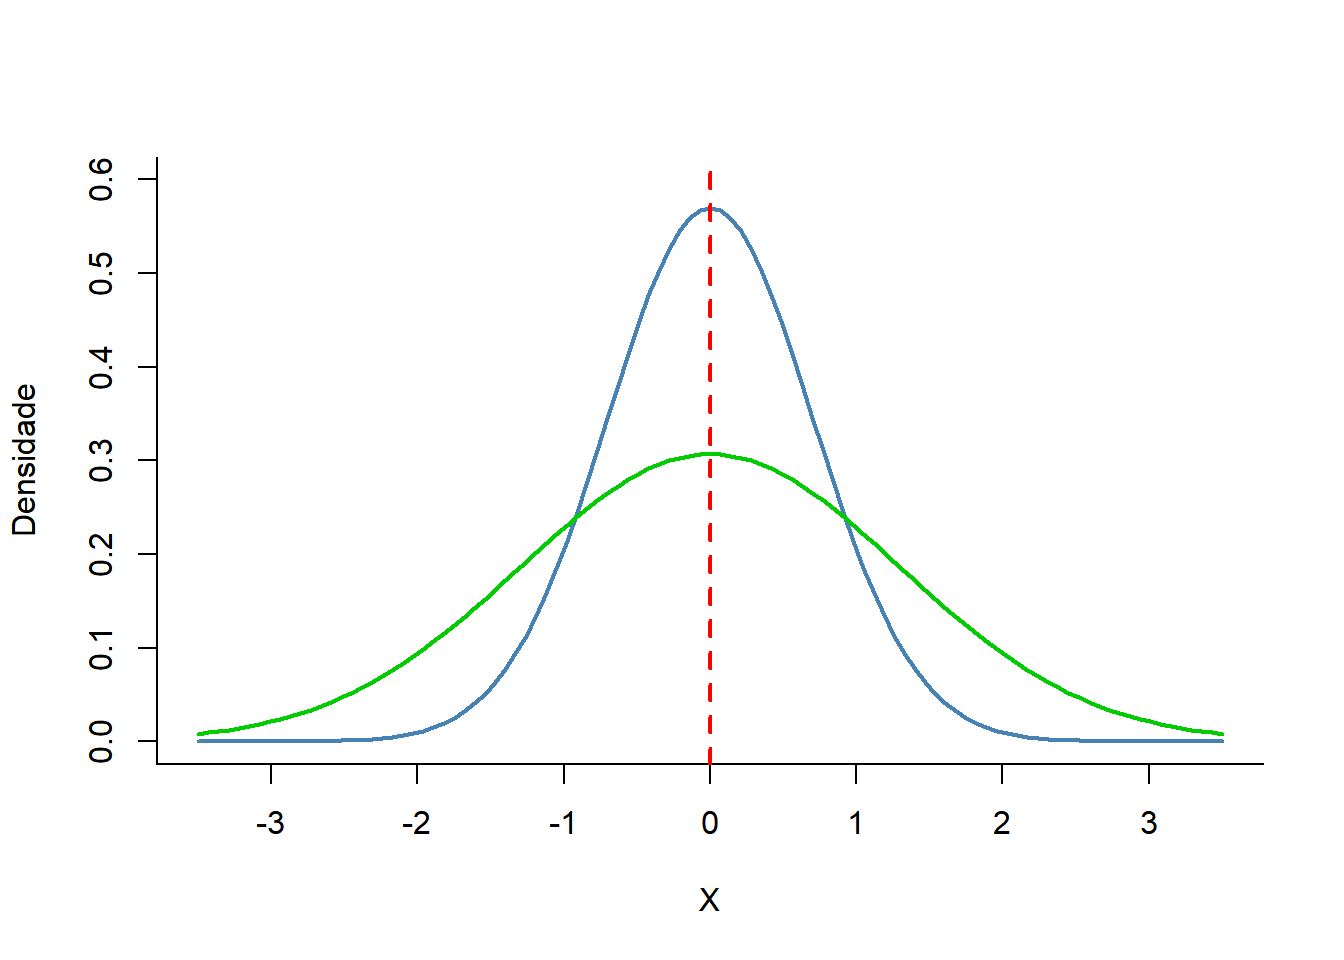
\includegraphics{bookdownproj_files/figure-latex/dispersao-1} 

}

\caption{Dispersão dos dados em torno da média.}\label{fig:dispersao}
\end{figure}

\subsubsection{Coeficiente de Variação}\label{coeficiente-de-variauxe7uxe3o}

O desvio padrão por si só tem limitações. Um desvio padrão de duas unidades pode ser considerado pequeno para um conjunto de valores cuja média é 100. Entretanto, se a média for 5, ele se torna muito grande. Além disso, o desvio padrão por ser expresso na mesma unidade dos dados, não permite aplicá-lo na comparação de dois ou mais conjunto de dados que têm unidades diferentes.
Para eliminar essas limitações, é possível caracterizar a dispersão ou variabilidade dos dados em termos relativos, usando uma medida denominada Coeficiente de Variação (CV), também conhecido como como \emph{Desvio Padrão Relativo} ou \emph{Coeficiente de Variação de Pearson}. É expresso, em geral como uma porcentagem, sendo definido como a razão do desvio padrão pela média:

\[
CV = \frac{s}{\overline{x}}
\]

Multiplicando o valor da equação por 100 tem-se o CV percentual. O R não possui uma função específica para calcular o CV.

Foi criada uma função específica para isso,já multiplicada por 100.

\begin{Shaded}
\begin{Highlighting}[]
\NormalTok{coef\_var }\OtherTok{\textless{}{-}} \ControlFlowTok{function}\NormalTok{ (valores) \{}
\NormalTok{  (}\FunctionTok{sd}\NormalTok{(valores, }\AttributeTok{na.rm=}\ConstantTok{TRUE}\NormalTok{) }\SpecialCharTok{/} \FunctionTok{mean}\NormalTok{(valores, }\AttributeTok{na.rm=}\ConstantTok{TRUE}\NormalTok{))}\SpecialCharTok{*}\DecValTok{100}\NormalTok{\}}
\end{Highlighting}
\end{Shaded}

Portanto, o CV da variável \texttt{dados\$pesoRN} é igual a:

\begin{Shaded}
\begin{Highlighting}[]
\FunctionTok{coef\_var}\NormalTok{ (dados}\SpecialCharTok{$}\NormalTok{pesoRN)}
\end{Highlighting}
\end{Shaded}

\begin{verbatim}
## [1] 13.79855
\end{verbatim}

Se usarmos outra variável do banco de dados, por exemplo, \texttt{dados\$idadeMae}, o CV será igual a:

\begin{Shaded}
\begin{Highlighting}[]
\FunctionTok{coef\_var}\NormalTok{ (dados}\SpecialCharTok{$}\NormalTok{idadeMae)}
\end{Highlighting}
\end{Shaded}

\begin{verbatim}
## [1] 21.37895
\end{verbatim}

O peso do recem-nascido tem um CV = 13.8 e a idade materna um CV = 21.4, mostrando que esta tem uma maior variabilidade. Quanto menor o desvio padrão, menor o CV e, consequentemente, menor a variabilidade. Um CV \(\ge\) 50\%, sugere que a variável tem uma distribuição assimétrica.

\subsection{Escolha da medida resumidora}\label{escolha-da-medida-resumidora}

A seleção da medida de tendência central mais adequada depende de vários fatores, incluindo a natureza dos dados e do propósito da sumarização.

O tipo da variável tem substancial influência na escolha da medida de tendência central a ser usada. A moda é mais apropriada para dados nominais e seu uso com variáveis ordinais resulta em uma perda no poder em termos de informação que se poderia obter dos dados.

A mediana é mais adequada para variáveis ordinais, embora possa ser usada para variáveis contínuas, especialmente quando a distribuição dos dados é assimétrica. A mediana não deveria ser usada com dados nominais porque os postos assumidos não podem ser obtidos com dados de nível nominal.

Finalmente, a média somente deve ser usada com dados contínuos simétricos, se houver assimetria a mediana deve ser preferida.

As medidas de dispersão devem estar associadas a uma medida de tendência central. Elas caracterizam a variabilidade dos dados na amostra. Com dados ordinais usar a amplitude ou o intervalo interquartil. O desvio padrão não é apropriado em dados ordinais devido à natureza não numérica destes.

Com os dados numéricos deve-se usar o desvio padrão, que utiliza toda a informação nos dados, ou o intervalo interquartil (IIQ). Quando os dados forem simétricos, usar a média acompanhada do desvio padrão, caso contrário, usar a mediana e o IIQ. Não misturar e combinar medidas \citep{bowers2008scratch}.

\section{Tabelas}\label{tabelas}

A apresentação tabular dos dados é a apresentação das informações por meio de tabelas. Uma tabela é uma forma eficiente de mostrar os dados levantados, facilitando a sua compreensão e interpretação. No R existem muitas maneira de criar tabelas.

\subsection{Dados usados nesta seção}\label{dados-usados-nesta-seuxe7uxe3o-1}

Para mostrar como construir as tabelas, será feita a leitura do conjunto de dados \texttt{dadosMater.xlsx}, mencionado na seção anterior . Como visto, este conjunto de dados contém uma grande quantidade colunas e, para tornar mais fácil a análise, serão selecionadas aquelas utilizadas nesta seção.

\begin{Shaded}
\begin{Highlighting}[]
\NormalTok{mater }\OtherTok{\textless{}{-}}\NormalTok{ readxl}\SpecialCharTok{::}\FunctionTok{read\_excel}\NormalTok{(}\StringTok{"Arquivos/dadosMater.xlsx"}\NormalTok{) }\SpecialCharTok{\%\textgreater{}\%} 
   \FunctionTok{select}\NormalTok{(idadeMae, altura, peso, anosEst, fumo, }
\NormalTok{           para, ig, sexo, pesoRN, compRN, utiNeo)}

\FunctionTok{str}\NormalTok{(mater)}
\end{Highlighting}
\end{Shaded}

\begin{verbatim}
## tibble [1,368 x 11] (S3: tbl_df/tbl/data.frame)
##  $ idadeMae: num [1:1368] 42 29 19 31 34 29 30 34 17 32 ...
##  $ altura  : num [1:1368] 1.65 1.66 1.72 1.55 1.6 1.5 1.54 1.63 1.68 1.5 ...
##  $ peso    : num [1:1368] 69.9 78 81 74 60 60 75.5 61 57 70 ...
##  $ anosEst : num [1:1368] 3 11 9 5 7 8 4 6 10 1 ...
##  $ fumo    : num [1:1368] 2 2 2 2 2 1 1 2 2 2 ...
##  $ para    : num [1:1368] 5 0 0 1 2 1 2 1 0 4 ...
##  $ ig      : num [1:1368] 29 33 33 33 33 33 33 33 34 34 ...
##  $ sexo    : num [1:1368] 2 2 2 2 2 2 2 2 2 2 ...
##  $ pesoRN  : num [1:1368] 1035 2300 1580 1840 2475 ...
##  $ compRN  : num [1:1368] 35.5 45 39 41 47 41 44 44 47 48 ...
##  $ utiNeo  : num [1:1368] 1 2 1 1 1 1 2 2 1 1 ...
\end{verbatim}

\subsection{Tabelas de Frequência}\label{sec-freq}

\subsubsection{Tabela de frequência para dados categóricos}\label{tabela-de-frequuxeancia-para-dados-categuxf3ricos}

Uma maneira concisa que permite observar a variável e extrair informação sobre o seu comportamento, é a utilização de uma \emph{tabela de frequência}. A tabela de frequência deve ser simples, clara e objetiva, ou seja, não deve ter um volume muito grande de informações. Deve ser autoexplicativa, não deve haver necessidade de ler o texto para entendê-la.

A tabela de frequência agrupa os dados por categorias ou classes, contabilizando o número ocorrências em cada categoria. O número de observações em uma determinada classe recebe o nome de \emph{frequência absoluta} (\emph{f}). Além da frequência absoluta, costuma aparecer a frequência relativa (\emph{fr}) que representa a proporção da classe em relação ao número total de observações (\emph{n}), calculada por \(fr = \frac{f}{n}\), a frequência percentual (\emph{fp}), obtida pela multiplicação da frequência relativa por 100 e a frequência acumulada, que é a soma de todas as classes até a classe atual, podendo ser frequência acumulada absoluta (\emph{F}), frequência acumulada relativa (\emph{Fr}) ou frequência acumulada percentual (\emph{Fp}).

Em uma tabela, os dados são apresentados em colunas verticais indicadoras e linhas horizontais. Nas linhas aparecem as categorias e nas colunas as frequências, constituindo o corpo da tabela. O cabeçalho indica a natureza do conteúdo de cada coluna. No cruzamento das colunas e das linhas, tem-se as caselas ou casas.

Existem algumas recomendações na construção de uma tabela de frequência \citet{arango2009tab}:

\begin{itemize}
\tightlist
\item
  deve ter um título na parte superior que responda as perguntas: ``o que? quando? onde?'' relativas ao fato estudado;
\item
  deve ter um rodapé, na parte inferior da tabela, onde se coloca notas necessárias e a fonte dos dados;
\item
  as colunas externas da tabela devem ser abertas, o emprego de linhas verticais para a separação das colunas no corpo da tabela é opcional;
\item
  Na parte superior e inferior, as tabelas devem, ser fechadas por linhas horizontais;
\item
  Nenhuma casela deve ficar vazia, apresentando um número ou um símbolo. Se não se dispuser do dado, colocar reticências \ldots{} e a presença de um X representa que o dado foi omitido para evitar a identificação.
\end{itemize}

Se os dados forem nominais, a ordenação das categorias é arbitrária, costuma-se colocar em primeiro lugar a maior frequência (Tabela \ref{tab:droga}) , colocando-os em categorias ordenadas \citep{oliveira2022tab}.

\begin{table}
\centering
\caption{\label{tab:droga}Distribuição de frequência de drogadição em parturientes do Hospital Geral de Caxias do Sul, RS, 2008.}
\centering
\begin{tabu} to \linewidth {>{\raggedright}X>{\raggedleft}X>{\raggedleft}X>{\raggedleft}X>{\raggedleft}X}
\toprule
\textbf{Drogadição} & \textbf{f} & \textbf{fr} & \textbf{fp} & \textbf{Fp}\\
\midrule
Não drogaditas & 904 & 0,955 & 95,5 & 95.5\\
Medicamentos & 23 & 0,024 & 2,4 & 97.9\\
Álcool & 17 & 0,018 & 1,8 & 99.7\\
Crack & 2 & 0,002 & 0,2 & 99.9\\
Cocaína & 1 & 0,001 & 0,1 & 100\\
\addlinespace
Total & 947 & 1,000 & 100,0 & \\
\bottomrule
\end{tabu}
\end{table}

\subsubsection{Construção da tabela de frequência}\label{sec-tabfreq}

Para demonstrar como construir uma tabela de frequência, usando o R, será usada uma variável categórica que não existe no conjunto de dados \texttt{mater.} Esta variável vai ser criada, categorizando a variável numérica \texttt{idadeMae} (idade da parturiente) em três categoria, classicamente, usadas: menores de 20 anos (adolescentes), 20 a 35 anos e maiores de 35 anos. No conjunto mater, a variável \texttt{idadeMae} tem como idade mínima 13 anos e idade máxima 46 anos. A nova variável receberá o nome de \texttt{categIdade}.
Para realizar este trabalho de transformação da variável numérica em categórica, será usada a função \texttt{cut()} do pacote R base.
Esta função tem vários argumentos:

\begin{itemize}
\tightlist
\item
  \emph{x} \(\longrightarrow\) vetor numérico
\item
  \emph{breaks} \(\longrightarrow\) vetor numérico de dois ou mais pontos de corte exclusivos ou um único número (maior ou igual a 2) dando o número de intervalos nos quais \emph{x} deve ser subdividido
\item
  \emph{labels} \(\longrightarrow\) rótulos para os níveis das categorias resultante. Por padrão, os rótulos são construídos usando a notação de intervalo \((a, b]\) (aberto à esquerda e fechado à direita).
\item
  \emph{include.lowest} \(\longrightarrow\) valor lógico, se o menor valor será incluido, ou o maior, se \texttt{right\ =\ TRUE}. Padrão = \texttt{include.lowest=TRUE}
\item
  \emph{right} \(\longrightarrow\) valor lógico indicando se o intervalo deve ser fechado à direita e aberto a esquerda. Padrão =
  \texttt{right\ =\ TRUE}.
\item
  \emph{ordered\_result} \(\longrightarrow\) valor lógico indicando se o resultado deve ser um fator ordenado.
\end{itemize}

\begin{Shaded}
\begin{Highlighting}[]
\NormalTok{mater}\SpecialCharTok{$}\NormalTok{categIdade }\OtherTok{\textless{}{-}} \FunctionTok{cut}\NormalTok{(mater}\SpecialCharTok{$}\NormalTok{idadeMae,}
                        \AttributeTok{breaks =} \FunctionTok{c}\NormalTok{(}\DecValTok{13}\NormalTok{, }\DecValTok{20}\NormalTok{, }\DecValTok{36}\NormalTok{, }\DecValTok{46}\NormalTok{),}
                        \AttributeTok{labels =} \FunctionTok{c}\NormalTok{(}\StringTok{"\textless{}20a"}\NormalTok{, }\StringTok{"20{-}35a"}\NormalTok{, }\StringTok{"\textgreater{}35a"}\NormalTok{),}
                        \AttributeTok{include.lowest =} \ConstantTok{TRUE}\NormalTok{,}
                        \AttributeTok{right =} \ConstantTok{FALSE}\NormalTok{,}
                        \AttributeTok{ordered\_result =}\ConstantTok{TRUE}\NormalTok{)}
\end{Highlighting}
\end{Shaded}

Para visualizar se a variável foi criada de maneira adequada, pode-se usar novamente a função \texttt{str()}:

\begin{Shaded}
\begin{Highlighting}[]
\FunctionTok{str}\NormalTok{(mater)}
\end{Highlighting}
\end{Shaded}

\begin{verbatim}
## tibble [1,368 x 12] (S3: tbl_df/tbl/data.frame)
##  $ idadeMae  : num [1:1368] 42 29 19 31 34 29 30 34 17 32 ...
##  $ altura    : num [1:1368] 1.65 1.66 1.72 1.55 1.6 1.5 1.54 1.63 1.68 1.5 ...
##  $ peso      : num [1:1368] 69.9 78 81 74 60 60 75.5 61 57 70 ...
##  $ anosEst   : num [1:1368] 3 11 9 5 7 8 4 6 10 1 ...
##  $ fumo      : num [1:1368] 2 2 2 2 2 1 1 2 2 2 ...
##  $ para      : num [1:1368] 5 0 0 1 2 1 2 1 0 4 ...
##  $ ig        : num [1:1368] 29 33 33 33 33 33 33 33 34 34 ...
##  $ sexo      : num [1:1368] 2 2 2 2 2 2 2 2 2 2 ...
##  $ pesoRN    : num [1:1368] 1035 2300 1580 1840 2475 ...
##  $ compRN    : num [1:1368] 35.5 45 39 41 47 41 44 44 47 48 ...
##  $ utiNeo    : num [1:1368] 1 2 1 1 1 1 2 2 1 1 ...
##  $ categIdade: Ord.factor w/ 3 levels "<20a"<"20-35a"<..: 3 2 1 2 2 2 2 2 1 2 ...
\end{verbatim}

A nova variável foi gerada de forma correta. Observe que para que isso acontecesse, foi usado \texttt{right\ =\ FALSE}, em consequência, o intervalo 13 a 20, incluirá o 13 (menor idade) e excluirá o 20, o intervalo 20 a 36, incluirá o 20 e excluirá o 36 e o último intervalo incluirá o 36 e excluirá o 46, que é o valor mais alto. Em função disso, foi incluído mais um argumento \texttt{include.lowest=TRUE}, para incluir o valor 46.
Para se verificar como ficou a distribuição de frequência absoluta, constrói-se uma tabela, inicialmente com a função \texttt{table()}:

\begin{Shaded}
\begin{Highlighting}[]
\NormalTok{f\_abs }\OtherTok{\textless{}{-}} \FunctionTok{table}\NormalTok{ (mater}\SpecialCharTok{$}\NormalTok{categIdade)}
\NormalTok{f\_abs}
\end{Highlighting}
\end{Shaded}

\begin{verbatim}
## 
##   <20a 20-35a   >35a 
##    219    992    157
\end{verbatim}

As frequências relativas podem ser obtidas com a função \texttt{prop.table()}, Esta função será usada dentro da função \texttt{round()} para arredondar os valores para 3 dígitos.

\begin{Shaded}
\begin{Highlighting}[]
\NormalTok{f\_rel }\OtherTok{\textless{}{-}} \FunctionTok{round}\NormalTok{(}\FunctionTok{prop.table}\NormalTok{(f\_abs), }\DecValTok{3}\NormalTok{)}
\NormalTok{f\_rel}
\end{Highlighting}
\end{Shaded}

\begin{verbatim}
## 
##   <20a 20-35a   >35a 
##  0.160  0.725  0.115
\end{verbatim}

Multiplicando por 100 a \texttt{f\_rel}, tem-se a frequência percentual \texttt{f\_perc}. De novo, a operação será colocada dentro da função \texttt{round()}, arredondando o resultado para dois dígitos.

\begin{Shaded}
\begin{Highlighting}[]
\NormalTok{f\_perc }\OtherTok{\textless{}{-}} \FunctionTok{round}\NormalTok{(f\_rel}\SpecialCharTok{*}\DecValTok{100}\NormalTok{, }\DecValTok{2}\NormalTok{)}
\NormalTok{f\_perc}
\end{Highlighting}
\end{Shaded}

\begin{verbatim}
## 
##   <20a 20-35a   >35a 
##   16.0   72.5   11.5
\end{verbatim}

Para construir uma tabela simples no R, pode-se proceder da seguinte maneira:

\begin{Shaded}
\begin{Highlighting}[]
\CommentTok{\# Criando as colunas das tabelas com o total de cada uma delas}
\NormalTok{f\_abs }\OtherTok{\textless{}{-}} \FunctionTok{c}\NormalTok{ (f\_abs, }\FunctionTok{sum}\NormalTok{(f\_abs))}
\NormalTok{f\_rel }\OtherTok{\textless{}{-}} \FunctionTok{c}\NormalTok{ (f\_rel, }\FunctionTok{sum}\NormalTok{ (f\_rel))}
\NormalTok{f\_perc }\OtherTok{\textless{}{-}} \FunctionTok{c}\NormalTok{ (f\_perc, }\FunctionTok{sum}\NormalTok{ (f\_perc))}

\CommentTok{\# Criando a tabela inicial com a concatenação das coluna {-} função cbind()}
\NormalTok{tab1 }\OtherTok{\textless{}{-}} \FunctionTok{cbind}\NormalTok{(f\_abs,}
\NormalTok{              f\_rel ,}
\NormalTok{              f\_perc)}
\NormalTok{tab1}
\end{Highlighting}
\end{Shaded}

\begin{verbatim}
##        f_abs f_rel f_perc
## <20a     219 0.160   16.0
## 20-35a   992 0.725   72.5
## >35a     157 0.115   11.5
##         1368 1.000  100.0
\end{verbatim}

Transformando a tab1 em um dataframe, nomeando a linha 4 e renomeando as colunas para ficar com os nomes referidos no início da seção:

\begin{Shaded}
\begin{Highlighting}[]
\NormalTok{tab1 }\OtherTok{\textless{}{-}} \FunctionTok{as.data.frame}\NormalTok{(tab1)}
\FunctionTok{row.names}\NormalTok{(tab1)[}\DecValTok{4}\NormalTok{] }\OtherTok{\textless{}{-}}  \StringTok{"Total"}
\FunctionTok{colnames}\NormalTok{(tab1) }\OtherTok{\textless{}{-}} \FunctionTok{c}\NormalTok{(}\StringTok{"f"}\NormalTok{, }\StringTok{"fr"}\NormalTok{, }\StringTok{"fp"}\NormalTok{)}
\NormalTok{tab1}
\end{Highlighting}
\end{Shaded}

\begin{verbatim}
##           f    fr    fp
## <20a    219 0.160  16.0
## 20-35a  992 0.725  72.5
## >35a    157 0.115  11.5
## Total  1368 1.000 100.0
\end{verbatim}

Esta uma tabela simples que serve para visualizar as informações. Não serve para publicações. Para obter uma tabela simples, mas muito mais profissional (Tabela \ref{tab:tisch}) pode ser utilizada a função \texttt{kable()} do pacote \texttt{knitr} \citet{xie2018knitr}. Esta função possui um grande número de argumentos para personalizar a aparência das tabelas\footnote{Para maiores detalhes: \url{https://haozhu233.github.io/kableExtra/awesome_table_in_pdf.pdf} ou consulte a ajuda digitando no Console \texttt{?kable()} ou \texttt{help(kable)}.}:

\begin{itemize}
\tightlist
\item
  \emph{x} \(\rightarrow\) é um objeto do R, tipicamente uma matiz ou dataframe;
\item
  \emph{format} \(\rightarrow\) sequência de caracteres. Os valores possíveis são ''latex'', ``html'', ``pipe'', ``simple'';
\item
  \emph{digits} \(\rightarrow\) número máximo de dígitos para colunas numéricas, passado para \texttt{round()};
\item
  \emph{row.names} \(\rightarrow\)lógico: se deve incluir nomes de linhas. Por padrão, os nomes de linhas serão incluídos se rownames(x) não for NULL nem idêntico a \texttt{1:nrow(x)}.
\item
  \emph{col.names} \(\rightarrow\) vetor de caracteres de nomes de colunas a serem usados na tabela.;
\item
  \emph{align} \(\rightarrow\) alinhamento da coluna: um vetor de caracteres que consiste em ``l'' (esquerda), ``c''\,' (centro) e/ou ``r'' (direita). Por padrão ou se \texttt{align\ =\ NULL}, as colunas numéricas são alinhadas à direita e as outras colunas são alinhadas à esquerda.;
\item
  \emph{caption} \(\rightarrow\) título da tabela;
\item
  \ldots{} \(\rightarrow\) outros argumentos
\end{itemize}

Um pacote adicional, \texttt{kableExtra} \citet{zhu2021construct}, permite opções de formatação simples, melhorando o aspecto da tabela, utilizando-se o operador pipe \%\textgreater\%. O pacote \texttt{kableExtra} foi projetado para estender a funcionalidade básica das tabelas produzidas usando \texttt{knitr::kable()}. Podem ser acrescentadas várias das suas funções como \texttt{kable\_styling()} ou \texttt{kable\_classic()} para especificar estilos à tabela, como extensão da tabela, alinhamento, tipo e tamanho da fonte \footnote{Consulte \url{https://cran.r-project.org/web/packages/kableExtra/kableExtra.pdf}}.

\begin{Shaded}
\begin{Highlighting}[]
\NormalTok{knitr}\SpecialCharTok{::}\FunctionTok{kable}\NormalTok{(tab1,}
             \AttributeTok{booktabs =} \ConstantTok{TRUE}\NormalTok{,}
             \AttributeTok{caption =} \StringTok{"Distribuição das puérperas por faixa etária, Hospital Geral de Caxias do Sul, RS, 2008."}\NormalTok{,}
             \AttributeTok{format.args =} \FunctionTok{list}\NormalTok{(}\AttributeTok{decimal.mark =} \StringTok{","}\NormalTok{)) }\SpecialCharTok{\%\textgreater{}\%} 
\NormalTok{kableExtra}\SpecialCharTok{::}\FunctionTok{kable\_classic\_2}\NormalTok{(}\AttributeTok{full\_width =} \ConstantTok{FALSE}\NormalTok{, }
                            \AttributeTok{html\_font =} \StringTok{"Cambria"}\NormalTok{,}
                            \AttributeTok{position =} \StringTok{"center"}\NormalTok{) }\SpecialCharTok{\%\textgreater{}\%} 
\NormalTok{kableExtra}\SpecialCharTok{::}\FunctionTok{row\_spec}\NormalTok{(}\DecValTok{0}\NormalTok{, }\AttributeTok{bold =} \ConstantTok{TRUE}\NormalTok{) }\SpecialCharTok{\%\textgreater{}\%} 
\NormalTok{   kableExtra}\SpecialCharTok{::}\FunctionTok{column\_spec}\NormalTok{(}\DecValTok{1}\SpecialCharTok{:}\DecValTok{4}\NormalTok{, }
                           \AttributeTok{width =} \StringTok{"2.5cm"}\NormalTok{)}
\end{Highlighting}
\end{Shaded}

\begin{table}
\centering
\caption{\label{tab:tisch}Distribuição das puérperas por faixa etária, Hospital Geral de Caxias do Sul, RS, 2008.}
\centering
\begin{tabular}[t]{>{\raggedright\arraybackslash}p{2.5cm}>{\raggedleft\arraybackslash}p{2.5cm}>{\raggedleft\arraybackslash}p{2.5cm}>{\raggedleft\arraybackslash}p{2.5cm}}
\toprule
\textbf{ } & \textbf{f} & \textbf{fr} & \textbf{fp}\\
\midrule
<20a & 219 & 0,160 & 16,0\\
20-35a & 992 & 0,725 & 72,5\\
>35a & 157 & 0,115 & 11,5\\
Total & 1368 & 1,000 & 100,0\\
\bottomrule
\end{tabular}
\end{table}

\subsubsection{Tabela de frequência para dados numéricos}\label{tabela-de-frequuxeancia-para-dados-numuxe9ricos}

Como fazer a distribuição de frequência de uma variável contínua sem um critério pré-determinado para as classes?

Como exemplo, será usado, agora, o IMC pré-gestacional das parturientes do banco de dados \texttt{dadosMater.xlsx}). Esta variável não existe, tem-se apenas o peso e a altura e, portanto, com estes dados, ela pode ser criada:

\begin{Shaded}
\begin{Highlighting}[]
\NormalTok{mater}\SpecialCharTok{$}\NormalTok{imc }\OtherTok{\textless{}{-}} \FunctionTok{round}\NormalTok{(mater}\SpecialCharTok{$}\NormalTok{peso}\SpecialCharTok{/}\NormalTok{mater}\SpecialCharTok{$}\NormalTok{altura}\SpecialCharTok{\^{}}\DecValTok{2}\NormalTok{, }\DecValTok{1}\NormalTok{)}
\FunctionTok{str}\NormalTok{(mater)}
\end{Highlighting}
\end{Shaded}

\begin{verbatim}
## tibble [1,368 x 13] (S3: tbl_df/tbl/data.frame)
##  $ idadeMae  : num [1:1368] 42 29 19 31 34 29 30 34 17 32 ...
##  $ altura    : num [1:1368] 1.65 1.66 1.72 1.55 1.6 1.5 1.54 1.63 1.68 1.5 ...
##  $ peso      : num [1:1368] 69.9 78 81 74 60 60 75.5 61 57 70 ...
##  $ anosEst   : num [1:1368] 3 11 9 5 7 8 4 6 10 1 ...
##  $ fumo      : num [1:1368] 2 2 2 2 2 1 1 2 2 2 ...
##  $ para      : num [1:1368] 5 0 0 1 2 1 2 1 0 4 ...
##  $ ig        : num [1:1368] 29 33 33 33 33 33 33 33 34 34 ...
##  $ sexo      : num [1:1368] 2 2 2 2 2 2 2 2 2 2 ...
##  $ pesoRN    : num [1:1368] 1035 2300 1580 1840 2475 ...
##  $ compRN    : num [1:1368] 35.5 45 39 41 47 41 44 44 47 48 ...
##  $ utiNeo    : num [1:1368] 1 2 1 1 1 1 2 2 1 1 ...
##  $ categIdade: Ord.factor w/ 3 levels "<20a"<"20-35a"<..: 3 2 1 2 2 2 2 2 1 2 ...
##  $ imc       : num [1:1368] 25.7 28.3 27.4 30.8 23.4 26.7 31.8 23 20.2 31.1 ...
\end{verbatim}

A variável \texttt{imc} foi criada de forma adequada. Essa variável foi construida por questões didáticas como exercício de manipulação dos dados no R.
Bem! Após, isso, para verificar a sua distribuição, segue-se os seguintes passos:

\begin{enumerate}
\def\labelenumi{\arabic{enumi}.}
\tightlist
\item
  \emph{Estabelecimento do número de classes (k)}:
\end{enumerate}

Antes, as classes foram estabelecidas de acordo com algum critério. Em geral, quando não há um padrão pré-determinado, o número de classes é estabelecido de acordo com o tamanho da amostra. Este número pode ser escolhido lembrando-se das oscilações que ocorrem nos dados e do interesse do pesquisador em mostrar seus dados. Não existe uma regra totalmente eficiente para determinar o número de classes. É importante ter bom senso, de maneira que seja possível ver como os valores se distribuem.

Para a maioria dos dados, é recomendado e 8 a 20 classes, isto é, 8 \(\le\) k \(\le\) 20. Com poucas classes, perde-se precisão e, com muitas classes, a tabela torna-se muito extensa. Baseado na regra de Sturges , é sugerido usar a recomendação da Figura \ref{fig:sturges} \citep{arango2009classes}.

\begin{figure}[H]

{\centering \includegraphics[width=0.7\linewidth]{https://i.imgur.com/IXn5SNz} 

}

\caption{Número de classes baseado em Sturges}\label{fig:sturges}
\end{figure}

Para a variável \texttt{imc}, como existem 1368 observações, deve-se usar ao redor de 10 classes. Executando a função \texttt{nclass.Sturges\ ()}, abaixo, o número de classes é igual a:

\begin{Shaded}
\begin{Highlighting}[]
\NormalTok{k }\OtherTok{\textless{}{-}} \FunctionTok{nclass.Sturges}\NormalTok{ (mater}\SpecialCharTok{$}\NormalTok{imc)}
\NormalTok{k}
\end{Highlighting}
\end{Shaded}

\begin{verbatim}
## [1] 12
\end{verbatim}

\begin{enumerate}
\def\labelenumi{\arabic{enumi}.}
\setcounter{enumi}{1}
\tightlist
\item
  \emph{Amplitude e limites das classes}:
\end{enumerate}

A classe possui um limite inferior e um limite superior. O importante é que os limites dos intervalos sejam mutuamente exclusivos, isto cada valor deve ser representado em um único intervalo. Além disso, os intervalos devem ser exaustivos, isto é, devem conter todos os valores possíveis entre o valor mínimo e o máximo. O recomendado é que as classes sejam homogêneas, ou seja, tenham a mesma amplitude. A amplitude dos valores pode ser obtida com a função \texttt{range()}:

\begin{Shaded}
\begin{Highlighting}[]
\NormalTok{amplitude }\OtherTok{\textless{}{-}} \FunctionTok{range}\NormalTok{(mater}\SpecialCharTok{$}\NormalTok{imc) }
\NormalTok{amplitude }
\end{Highlighting}
\end{Shaded}

\begin{verbatim}
## [1] 11.8 48.7
\end{verbatim}

Usando esta amplitude dos dados, é possível ter a largura (amplitude) das classes (\texttt{h}), usando a diferença entre o mínimo e máximo e divdindo pelo número de clsasses (\texttt{k}):

\begin{Shaded}
\begin{Highlighting}[]
\NormalTok{h }\OtherTok{\textless{}{-}} \FunctionTok{round}\NormalTok{(}\FunctionTok{diff}\NormalTok{(amplitude)}\SpecialCharTok{/}\NormalTok{k, }\DecValTok{0}\NormalTok{)}
\NormalTok{h}
\end{Highlighting}
\end{Shaded}

\begin{verbatim}
## [1] 3
\end{verbatim}

A fórmula é apenas a diferença absoluta dos limites inferior e superior dividida pelo número de classes, arredondado com o a função round () com 1 dígito decimal.

A partir desses dados, é possível construir as classes. A primeira classe será o valor mínimo de 11,8, que pode ser arredondado para 11,8 até 14,8 (11,8 + 3) exclusive; a segunda classe será 14,8 até 17,8 (14,8 + 3) e assim por diante.

\begin{enumerate}
\def\labelenumi{\arabic{enumi}.}
\setcounter{enumi}{2}
\tightlist
\item
  \emph{Construção da tabela}:
\end{enumerate}

Pode-se construir a tabela, usando a função \texttt{table()} e dentro desta a função \texttt{cut()} e dentro dela a função \texttt{seq(limite\ inferior,\ limite\ superior,\ l\ =\ número\ de\ classes)}.

\begin{Shaded}
\begin{Highlighting}[]
\NormalTok{categImc }\OtherTok{\textless{}{-}} \FunctionTok{table}\NormalTok{(}\FunctionTok{cut}\NormalTok{(mater}\SpecialCharTok{$}\NormalTok{imc,}
                        \AttributeTok{rigth =} \ConstantTok{TRUE}\NormalTok{,}
                        \AttributeTok{include.lowest =} \ConstantTok{TRUE}\NormalTok{,}
                        \FunctionTok{seq}\NormalTok{(}\FloatTok{11.8}\NormalTok{, }\FloatTok{48.7}\NormalTok{, }\AttributeTok{l =}\NormalTok{ k }\SpecialCharTok{+} \DecValTok{1}\NormalTok{)))}
\NormalTok{categImc}
\end{Highlighting}
\end{Shaded}

\begin{verbatim}
## 
## [11.8,14.9]   (14.9,18]     (18,21]   (21,24.1] (24.1,27.2] (27.2,30.3] 
##           2          46         258         480         237         176 
## (30.3,33.3] (33.3,36.4] (36.4,39.5] (39.5,42.6] (42.6,45.6] (45.6,48.7] 
##          87          39          22          12           5           4
\end{verbatim}

Preste atenção! Estes comandos que vão gerar a tabela têm o argumento \texttt{right\ =\ TRUE\ (padrão)}. Neste caso, ao contrário do comentado anteriormente, onde foi usado \texttt{right\ =\ FALSE}, os símbolos aparecem como ({]} (na tabela) e significa que o limite inferior da classe foi excluído (aberto à esquerda) e o superior foi incluído (fechado à direita). Aqui, também foi introduzido o argumento \texttt{include.lowest\ \ =\ TRUE} para incluir o valor mínimo dos dados (11,8), e a representação gráfica fica {[}{]}.

Olhando a saída do objeto \texttt{nutriCateg}, ela parece pouco esclarecedora e, no caso do IMC, talvez fosse melhor usar outro critério. Como por exemplo o que define o estado nutricional no 1° trimestre de gestação e classifica as gestantes em \emph{baixo peso} (IMC \(<\) 18,5 kg/\(m^2\)), \emph{peso adequado} (18,5 \(\le\) IMC \(\le\) 24,9 kg/\(m^2\)), \emph{sobrepeso} (25,0 \(\le\) IMC \(\le\) 29,9 kg/\(m^2\)) e \emph{obesidade} (IMC \(\ge\) 30 kg/\(m^2\)). Assim, é recomendado um ganho de peso total adequado de 12,5 kg a 18 kg para as gestantes classificadas como baixo peso; de 11,5 kg a 16,0 kg para as classificadas como peso adequado; de 7,0 a 11,5 kg nas classificadas com sobrepeso; e de 5,0 a 9,0 kg nas obesas \citep{rasmussen2009weight}.

\begin{Shaded}
\begin{Highlighting}[]
\NormalTok{mater}\SpecialCharTok{$}\NormalTok{estNutri }\OtherTok{\textless{}{-}} \FunctionTok{cut}\NormalTok{(mater}\SpecialCharTok{$}\NormalTok{imc,}
                      \AttributeTok{breaks =} \FunctionTok{c}\NormalTok{(}\FloatTok{11.8}\NormalTok{, }\FloatTok{18.5}\NormalTok{, }\DecValTok{25}\NormalTok{, }\DecValTok{30}\NormalTok{, }\FloatTok{48.7}\NormalTok{),}
                      \AttributeTok{labels =} \FunctionTok{c}\NormalTok{(}\StringTok{"Baixo Peso"}\NormalTok{, }\StringTok{"Peso adequado"}\NormalTok{, }
                                 \StringTok{"Sobrepeso"}\NormalTok{, }\StringTok{"Obesidade"}\NormalTok{),}
                      \AttributeTok{include.lowest =} \ConstantTok{TRUE}\NormalTok{,}
                      \AttributeTok{right =} \ConstantTok{FALSE}\NormalTok{,}
                      \AttributeTok{ordered\_result =}\ConstantTok{TRUE}\NormalTok{)}
\end{Highlighting}
\end{Shaded}

Isto cria uma nova variável \texttt{estNutri} (estado nutricional), no conjunto de dados mater, com 4 níveis (baixo Peso, Peso adequado, sobrepeso e Obesidade). Desta forma, pode-se construir uma tabela que melhor define este grupo de mulheres quanto ao estado nutricional.

\begin{Shaded}
\begin{Highlighting}[]
\NormalTok{f.abs }\OtherTok{\textless{}{-}} \FunctionTok{table}\NormalTok{ (mater}\SpecialCharTok{$}\NormalTok{estNutri)}
\NormalTok{f.rel }\OtherTok{\textless{}{-}} \FunctionTok{round}\NormalTok{(}\FunctionTok{prop.table}\NormalTok{(f.abs), }\DecValTok{3}\NormalTok{)}
\NormalTok{f.perc }\OtherTok{\textless{}{-}} \FunctionTok{round}\NormalTok{(f.rel}\SpecialCharTok{*}\DecValTok{100}\NormalTok{, }\DecValTok{2}\NormalTok{)}

\NormalTok{f.abs }\OtherTok{\textless{}{-}} \FunctionTok{c}\NormalTok{ (f.abs, }\FunctionTok{sum}\NormalTok{(f.abs))}
\NormalTok{f.rel }\OtherTok{\textless{}{-}} \FunctionTok{c}\NormalTok{ (f.rel, }\FunctionTok{sum}\NormalTok{ (f.rel))}
\NormalTok{f.perc }\OtherTok{\textless{}{-}} \FunctionTok{c}\NormalTok{ (f.perc, }\FunctionTok{sum}\NormalTok{ (f.perc))}

\NormalTok{tab2 }\OtherTok{\textless{}{-}} \FunctionTok{cbind}\NormalTok{(f.abs,}
\NormalTok{              f.rel ,}
\NormalTok{              f.perc)}

\NormalTok{tab2 }\OtherTok{\textless{}{-}} \FunctionTok{as.data.frame}\NormalTok{(tab2)}
\FunctionTok{row.names}\NormalTok{(tab2)[}\DecValTok{5}\NormalTok{] }\OtherTok{\textless{}{-}}  \StringTok{"Total"}
\FunctionTok{colnames}\NormalTok{(tab2) }\OtherTok{\textless{}{-}} \FunctionTok{c}\NormalTok{(}\StringTok{"f"}\NormalTok{, }\StringTok{"fr"}\NormalTok{, }\StringTok{"fp"}\NormalTok{)}
\NormalTok{tab2}
\end{Highlighting}
\end{Shaded}

\begin{verbatim}
##                  f    fr    fp
## Baixo Peso      67 0.049   4.9
## Peso adequado  791 0.578  57.8
## Sobrepeso      335 0.245  24.5
## Obesidade      175 0.128  12.8
## Total         1368 1.000 100.0
\end{verbatim}

Colocando em um formato mais científico, tem-se uma tabela (Tabela \ref{tab:aripaka}) bem mais elegante sobre o estado nutricional pré-gestacional:

\begin{Shaded}
\begin{Highlighting}[]
\NormalTok{knitr}\SpecialCharTok{::}\FunctionTok{kable}\NormalTok{(tab2,}
             \AttributeTok{booktabs =} \ConstantTok{TRUE}\NormalTok{,}
             \AttributeTok{caption =} \StringTok{"Estado nutricional pré{-}gestacional das parturientes, HGCS, 2008."}\NormalTok{,}
             \AttributeTok{format.args =} \FunctionTok{list}\NormalTok{(}\AttributeTok{decimal.mark =} \StringTok{","}\NormalTok{)) }\SpecialCharTok{\%\textgreater{}\%} 
\NormalTok{kableExtra}\SpecialCharTok{::}\FunctionTok{kable\_classic\_2}\NormalTok{(}\AttributeTok{full\_width =} \ConstantTok{TRUE}\NormalTok{,}
                            \AttributeTok{html\_font =} \StringTok{"Cambria"}\NormalTok{,}
                            \AttributeTok{position =} \StringTok{"center"}\NormalTok{) }\SpecialCharTok{\%\textgreater{}\%} 
\NormalTok{kableExtra}\SpecialCharTok{::}\FunctionTok{row\_spec}\NormalTok{(}\DecValTok{0}\NormalTok{, }\AttributeTok{bold =} \ConstantTok{TRUE}\NormalTok{) }\SpecialCharTok{\%\textgreater{}\%} 
\NormalTok{kableExtra}\SpecialCharTok{::}\FunctionTok{column\_spec}\NormalTok{(}\DecValTok{1}\NormalTok{, }\AttributeTok{width =} \StringTok{"3.5cm"}\NormalTok{)  }\SpecialCharTok{\%\textgreater{}\%} 
\NormalTok{kableExtra}\SpecialCharTok{::}\FunctionTok{column\_spec}\NormalTok{(}\DecValTok{2}\SpecialCharTok{:}\DecValTok{4}\NormalTok{, }\AttributeTok{width =} \StringTok{"2.5cm"}\NormalTok{)  }
\end{Highlighting}
\end{Shaded}

\begin{table}
\centering
\caption{\label{tab:aripaka}Estado nutricional pré-gestacional das parturientes, HGCS, 2008.}
\centering
\begin{tabu} to \linewidth {>{\raggedright\arraybackslash}p{3.5cm}>{\raggedleft\arraybackslash}p{2.5cm}>{\raggedleft\arraybackslash}p{2.5cm}>{\raggedleft\arraybackslash}p{2.5cm}}
\toprule
\textbf{ } & \textbf{f} & \textbf{fr} & \textbf{fp}\\
\midrule
Baixo Peso & 67 & 0,049 & 4,9\\
Peso adequado & 791 & 0,578 & 57,8\\
Sobrepeso & 335 & 0,245 & 24,5\\
Obesidade & 175 & 0,128 & 12,8\\
Total & 1368 & 1,000 & 100,0\\
\bottomrule
\end{tabu}
\end{table}

\subsection{Tabelas de contingência}\label{tabelas-de-continguxeancia}

As tabelas de contingência, também chamadas tabelas cruzadas, são bastante usadas em estatísticas epidemiológicas para resumir a relação entre duas ou mais variáveis categóricas.

Uma tabela de contingência é um tipo especial de tabela de distribuição de frequência, onde duas variáveis são mostradas simultaneamente. Por exemplo, um pesquisador pode estar interessado em saber se o hábito de fumar na gestação aumenta o risco de o recém-nascido precisar de cuidados intensivos.\\
Existem duas variáveis \texttt{fumo} (fumo na gestação) e \texttt{utiNeo} (necessidade de cuidados intensivos neonatais) no banco de dados \texttt{dadosMater.xlsx}. Cada uma dessas variáveis tem duas alternativas, \texttt{sim} e \texttt{não}, por isso a tabela de cruzamento é denominada tabela de contingência 2 x 2. No arquivo, estão registradas como variáveis numéricas , 1 e 2, e devem ser transformadas para fatores (1 = sim e 2 = não)\footnote{Poderiam ser transformados em fatores sem trocar os rótulos e manter os números 1 e 2, como se fossem palavras. O autor prefere usar nomes.}, usando a função \texttt{factor()}.

\begin{Shaded}
\begin{Highlighting}[]
\NormalTok{mater}\SpecialCharTok{$}\NormalTok{fumo }\OtherTok{\textless{}{-}} \FunctionTok{factor}\NormalTok{ (mater}\SpecialCharTok{$}\NormalTok{fumo, }
                      \AttributeTok{ordered =} \ConstantTok{TRUE}\NormalTok{, }
                      \AttributeTok{levels =} \FunctionTok{c}\NormalTok{ (}\DecValTok{1}\NormalTok{,}\DecValTok{2}\NormalTok{), }
                      \AttributeTok{labels =} \FunctionTok{c}\NormalTok{ (}\StringTok{"sim"}\NormalTok{, }\StringTok{"não"}\NormalTok{))}
\NormalTok{mater}\SpecialCharTok{$}\NormalTok{utiNeo }\OtherTok{\textless{}{-}} \FunctionTok{factor}\NormalTok{ (mater}\SpecialCharTok{$}\NormalTok{utiNeo, }
                        \AttributeTok{ordered =} \ConstantTok{TRUE}\NormalTok{, }
                        \AttributeTok{levels =} \FunctionTok{c}\NormalTok{ (}\DecValTok{1}\NormalTok{,}\DecValTok{2}\NormalTok{), }
                        \AttributeTok{labels =} \FunctionTok{c}\NormalTok{ (}\StringTok{"sim"}\NormalTok{, }\StringTok{"não"}\NormalTok{))}
\end{Highlighting}
\end{Shaded}

Basta agora, usar a função \texttt{with()} junto com a função \texttt{table(variável\ da\ linha,\ variável\ das\ colunas)}. Por convenção, costuma-se colocar a variável explicativa ou explanatória nas linhas (\texttt{fumo}) e o desfecho nas colunas (\texttt{utiNeo}):

\begin{Shaded}
\begin{Highlighting}[]
\NormalTok{tabFumo }\OtherTok{\textless{}{-}} \FunctionTok{with}\NormalTok{(}\AttributeTok{data =}\NormalTok{ mater, }\FunctionTok{table}\NormalTok{(fumo, utiNeo))}
\NormalTok{tabFumo}
\end{Highlighting}
\end{Shaded}

\begin{verbatim}
##      utiNeo
## fumo  sim não
##   sim  71 230
##   não 204 863
\end{verbatim}

Para ter a soma das margens, usar a função \texttt{addmargins\ (tabela,\ margin\ =\ c\ (1,2),\ FUN\ =\ sum)} do pacote \texttt{stats}, incluído na instalação básica do R. A função adiciona a soma das linhas (1) e das colunas (2) às margens da tabela (\texttt{tabFumo}).

\begin{Shaded}
\begin{Highlighting}[]
\FunctionTok{addmargins}\NormalTok{ (tabFumo, }\AttributeTok{margin =} \FunctionTok{c}\NormalTok{(}\DecValTok{1}\NormalTok{,}\DecValTok{2}\NormalTok{), }\AttributeTok{FUN =}\NormalTok{ sum)}
\end{Highlighting}
\end{Shaded}

\begin{verbatim}
## Margins computed over dimensions
## in the following order:
## 1: fumo
## 2: utiNeo
\end{verbatim}

\begin{verbatim}
##      utiNeo
## fumo   sim  não  sum
##   sim   71  230  301
##   não  204  863 1067
##   sum  275 1093 1368
\end{verbatim}

Observando a tabela de contingência, verifica-se que a proporção entre as gestantes fumantes de internação na UTI neonatal foi 71/301 = 0,236 e entre as não fumantes foi de 204/1067 = 0,191. Para verificar se esta diferença ocorreu por acaso ou ela é significativa, há necessidade de se realizar um teste de hipótese, o qui-quadrado, que será visto no Capítulo 16.

\section{Gráficos}\label{gruxe1ficos}

Para descrever os dados e visualizar o que está acontecendo, recomenda-se utilizar um gráfico adequado. O que é adequado depende principalmente do tipo de dados, bem como das características particulares do que se quer explorar. Além disso, um gráfico em um relatório sempre é um fator de ``impacto''. Ou seja, pode ter um efeito positivo no leitor ou fazê-lo abandonar a leitura. Finalmente, um gráfico de frequência pode ser utilizado para ilustrar, explicar uma situação complexa onde palavras ou uma tabela podem ser confusos, extensos ou de outro modo insuficiente. Por outro lado, deve-se evitar usar gráficos onde poucas palavras expressam claramente o que se quer mostrar. Aconselha-se que, ao analisar os dados, é importante inspecioná-los como se fossem uma imagem, uma fotografia, ver como eles se parecem, qual o seu aspecto, e só então pensar em interpretar os aspectos vitais da estatística \citep{field2012graphs}.

O R básico fornece uma grande variedade de funções para visualizar dados, elas de uma maneira relativamente simples permitem a construção de gráficos que facilitam a interpretação tanto de variáveis categórica como contínuas. Para gráficos mais sofisticados existe um pacote denominado \texttt{ggplot2} \citep{wickham2016getting}. Este pacote é uma ferramenta extremamente versátil. É um pouco mais complexo e exige mais tempo para dominá-lo, mas, uma vez que se aprenda o básico sobre ele, oferece uma estrutura extremamente flexível para exibir os dados . Inicialmente, serão usadas as funções do R básico e,posteriormente, será feita uma introdução ao \texttt{ggplot2} (seção \ref{sec-ggplot2}).

\subsection{Gráfico de setores}\label{gruxe1fico-de-setores}

Também conhecido como gráfico de \emph{pizza}. Cada segmento (fatia) do gráfico de pizza deve ser proporcional à frequência da categoria que representa. A desvantagem do gráfico de pizza é que ele só pode representar uma variável, portanto, há necessidade de um gráfico separado para cada variável que se deseja representar. Além disso, um gráfico de pizza pode perder clareza se ele é usado para representar mais do que quatro ou cinco categorias. Na maioria das vezes, em um artigo ou relatório não há necessidade de se usar este tipo de gráfico. As tabelas são muito melhores. Segundo Edward Tufte, professor emérito de estatística, \emph{design} gráfico e economia política na Universidade de Yale, o único gráfico pior do que um gráfico de pizza são vários deles \citep{tufte2001aesthetics}! Ele é usado mais no mundo dos negócios. Como regra, não use gráfico de pizza!

Em uma consulta, entre estudantes de Medicina, foi perguntado a sua opinião em relação a este tipo de gráfico. A pergunta feita foi: ``O que você sente ao ver um gráfico de pizza em um artigo científico?'' As alternativas para a resposta eram quatro (ódio, irritação, indiferença, amor). O resultado do inquérito está na Tabela \ref{tab:pizza}.

\begin{table}
\centering
\caption{\label{tab:pizza}Sentimento dos alunos de Medicina em relação ao gráfico de pizza, UCS, 2012.}
\centering
\begin{tabular}[t]{>{\raggedright\arraybackslash}p{3.5cm}|>{\raggedleft\arraybackslash}p{1.5cm}|>{\raggedleft\arraybackslash}p{1.5cm}|>{\raggedleft\arraybackslash}p{1.5cm}|>{\raggedleft\arraybackslash}p{1.5cm}}
\hline
\textbf{Sentimento} & \textbf{f} & \textbf{fr} & \textbf{fp} & \textbf{Fp}\\
\hline
Odeiam & 6 & 0,15 & 15 & 15\\
\hline
Não gostam & 12 & 0,30 & 30 & 45\\
\hline
Indiferentes & 14 & 0,35 & 35 & 80\\
\hline
Amam & 8 & 0,20 & 20 & 100\\
\hline
Total & 40 & 1,00 & 100 & \\
\hline
\end{tabular}
\end{table}

No R base, pacote \texttt{graphics}, existe a função \texttt{pie()}para obter um gráfico de setores simples. Esta função usa os seguintes argumentos basicos, consulte a ajuda do R para outras informações:

\begin{itemize}
\tightlist
\item
  \emph{x} \(\longrightarrow\) vetor numérico não negativo\\
\item
  \emph{labels} \(\longrightarrow\) caracteres que fornecem nomes para as fatias. Para rótulos vazios ou NA (após coerção para caractere), nenhum rótulo ou linha indicadora é desenhada\\
\item
  \emph{radius} \(\longrightarrow\) A pizza é desenhada centralizada em um quadrado cujos lados variam de -1 a +1. Se os caracteres que rotulam as fatias forem longos, pode ser necessário usar um raio menor. O padrão é 0,8.\\
\item
  \emph{density} \(\longrightarrow\) Densidade das linhas de sombreamento, em linhas por polegada. O padrão é NULL significa que nenhuma linha de sombreamento é desenhada. Valores não positivos de densidade também inibem o desenho de linhas sombreadas
\item
  \emph{col} \(\longrightarrow\) Vetor de cores a ser usado no preenchimento ou sombreamento das fatias. Se estiver faltando, um conjunto de 6 cores pastel é usado
\end{itemize}

Os valores da coluna de frequência absoluta (\emph{f}) da Tabela \ref{tab:pizza} serão usados como o argumento \emph{x}. Ele informa a área (proporção de cada fatia. Os rótulos das fatias são escritos com a função concatenar \texttt{c()}.

\begin{Shaded}
\begin{Highlighting}[]
\FunctionTok{pie}\NormalTok{(}\AttributeTok{x =} \FunctionTok{c}\NormalTok{(}\DecValTok{6}\NormalTok{, }\DecValTok{12}\NormalTok{, }\DecValTok{14}\NormalTok{, }\DecValTok{8}\NormalTok{),}
    \AttributeTok{labels =} \FunctionTok{c}\NormalTok{(}\StringTok{"Odeiam"}\NormalTok{, }\StringTok{"Não gostam"}\NormalTok{, }\StringTok{"Indiferentes"}\NormalTok{, }\StringTok{"Amam"}\NormalTok{))}
\end{Highlighting}
\end{Shaded}

\begin{figure}[H]

{\centering 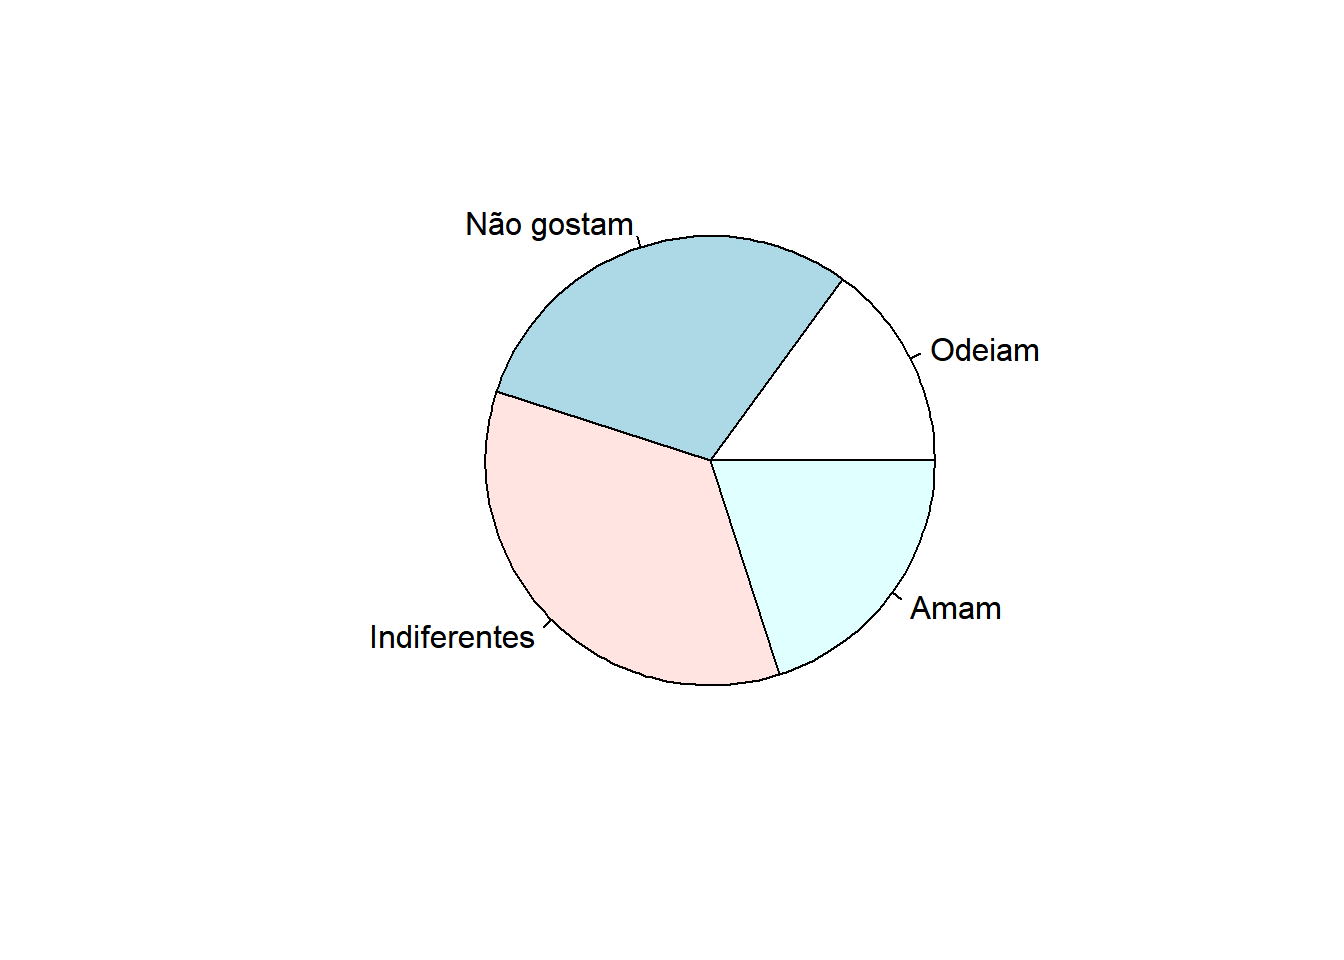
\includegraphics[width=1\linewidth,height=1\textheight]{bookdownproj_files/figure-latex/pie-1} 

}

\caption{Gráfico de Pizza: Opinião dos estudantes de Medicina.}\label{fig:pie}
\end{figure}

As cores que aparecem na Figura \ref{fig:pie} foram escolhidas pelo R, usando o seu padrão. Entretanto, elas podem ser customizadas, especificando-as pelo nome colocado entre parênteses. Por exemplo, \texttt{col\ =\ "red"} e se for mais de uma cor usar a função concatenar, \texttt{col\ =\ c(“gray58“,\ “yellow4”,\ “cyan”,\ “tomato”)}. As cores também podem se denotadas pelo sistemas RGB ou hexadecimal. A sigla RGB representa as cores primária em inglês (Red, Green, Blue). O código hexadecimal da cor branca é \#FFFFFFF, da gray58 é \#949494, da yellow4 é \#999900, da cyan é \#00FFFFe da tomato é \#FF6347 (Figura \ref{fig:pie2}).

\begin{Shaded}
\begin{Highlighting}[]
\FunctionTok{pie}\NormalTok{(}\AttributeTok{x =} \FunctionTok{c}\NormalTok{(}\DecValTok{6}\NormalTok{, }\DecValTok{12}\NormalTok{, }\DecValTok{14}\NormalTok{, }\DecValTok{8}\NormalTok{),}
    \AttributeTok{labels =} \FunctionTok{c}\NormalTok{(}\StringTok{"Odeiam"}\NormalTok{, }\StringTok{"Não gostam"}\NormalTok{, }\StringTok{"Indiferentes"}\NormalTok{, }\StringTok{"Amam"}\NormalTok{),}
    \AttributeTok{col =} \FunctionTok{c}\NormalTok{(}\StringTok{"gray58"}\NormalTok{, }\StringTok{"yellow4"}\NormalTok{, }\StringTok{"cyan"}\NormalTok{, }\StringTok{"tomato"}\NormalTok{))}
\end{Highlighting}
\end{Shaded}

\begin{figure}[H]

{\centering 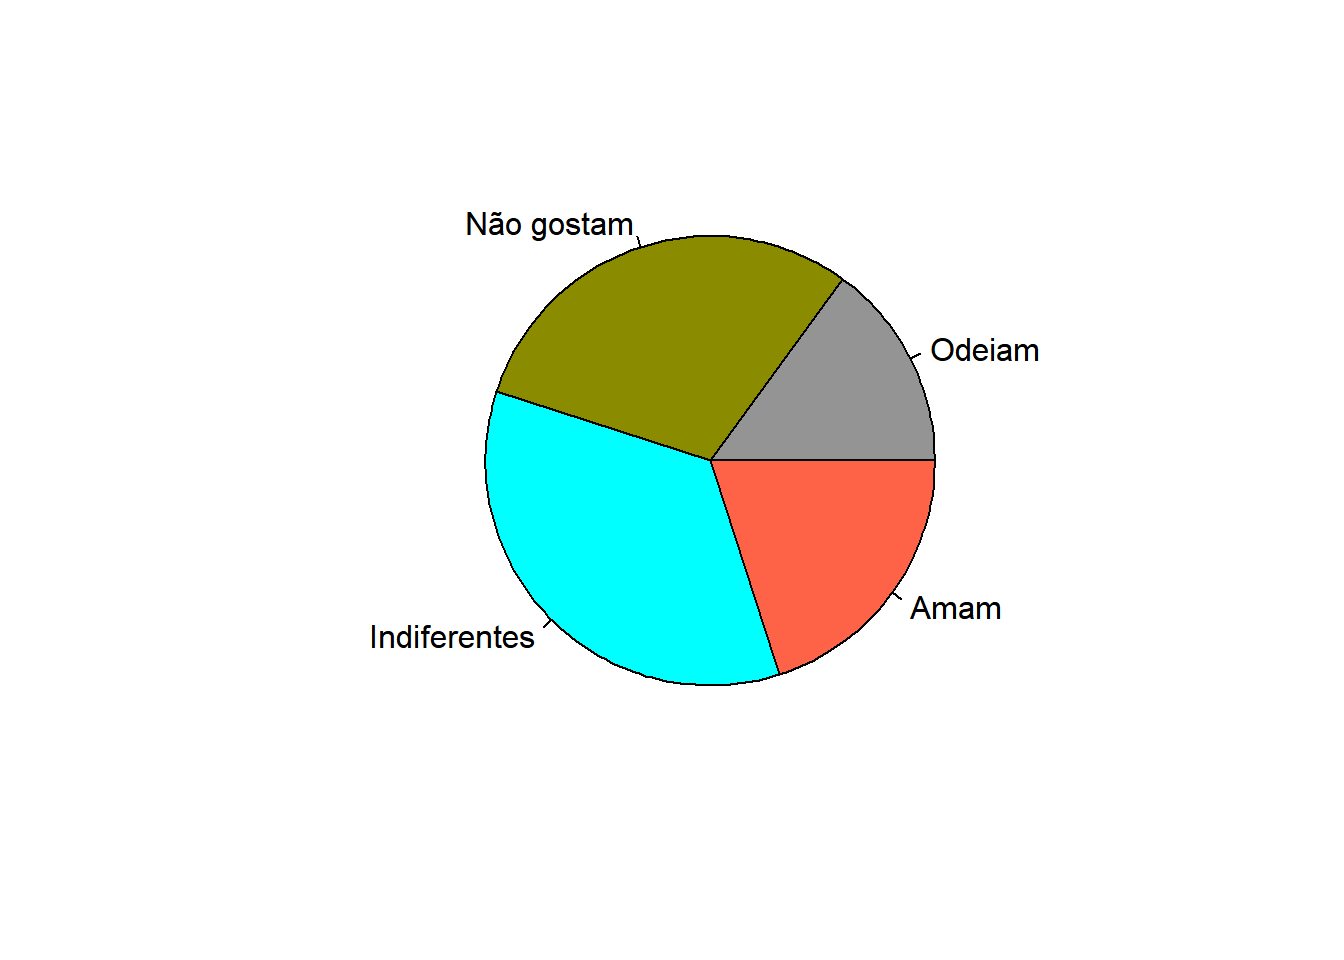
\includegraphics[width=1\linewidth,height=1\textheight]{bookdownproj_files/figure-latex/pie2-1} 

}

\caption{Figura anterior com cores personalizadas.}\label{fig:pie2}
\end{figure}

As cores parecem espetaculosas, mas o objetivo foi de criticar os gráficos tipo pista. Se o leitor quiser insistir no seu uso e com um gráfico em 3D (Figura \ref{fig:pie3d}), pode-se instalar o pacote \texttt{plotrix} (\citet{lemon2015package}) e carregar a função \texttt{pie3D()}. Os argumentos são praticamente os mesmos do gráfico simples. Acrescenta-se \texttt{radius\ =\ 0.9} que muda o raio da pizza e \texttt{explode\ =\ 0.1} que determina o afastamento das fatias (0, as mantém juntas). Além disso, como o gráfico exibe rótulos com textos muito grandes, usa-se o argumento \texttt{labelcex\ =\ 1}. Como qualquer função nova, basta clicar na tecla \emph{Tab}, dentro da mesma, que aparece um menu com as alternativas de argumentos.

\begin{Shaded}
\begin{Highlighting}[]
\FunctionTok{library}\NormalTok{ (plotrix)}

\FunctionTok{pie3D}\NormalTok{(}\AttributeTok{x =} \FunctionTok{c}\NormalTok{(}\DecValTok{6}\NormalTok{, }\DecValTok{12}\NormalTok{, }\DecValTok{14}\NormalTok{, }\DecValTok{8}\NormalTok{),}
    \AttributeTok{labels =} \FunctionTok{c}\NormalTok{(}\StringTok{"Odeiam"}\NormalTok{, }\StringTok{"Não gostam"}\NormalTok{, }\StringTok{"Indiferentes"}\NormalTok{, }\StringTok{"Amam"}\NormalTok{),}
    \AttributeTok{radius =} \FloatTok{0.9}\NormalTok{,}
    \AttributeTok{explode =} \FloatTok{0.1}\NormalTok{,}
    \AttributeTok{col =} \FunctionTok{c}\NormalTok{(}\StringTok{"gray58"}\NormalTok{, }\StringTok{"yellow4"}\NormalTok{, }\StringTok{"cyan"}\NormalTok{, }\StringTok{"tomato"}\NormalTok{),}
    \AttributeTok{labelcex =} \DecValTok{1}\NormalTok{)}
\end{Highlighting}
\end{Shaded}

\begin{figure}[H]

{\centering 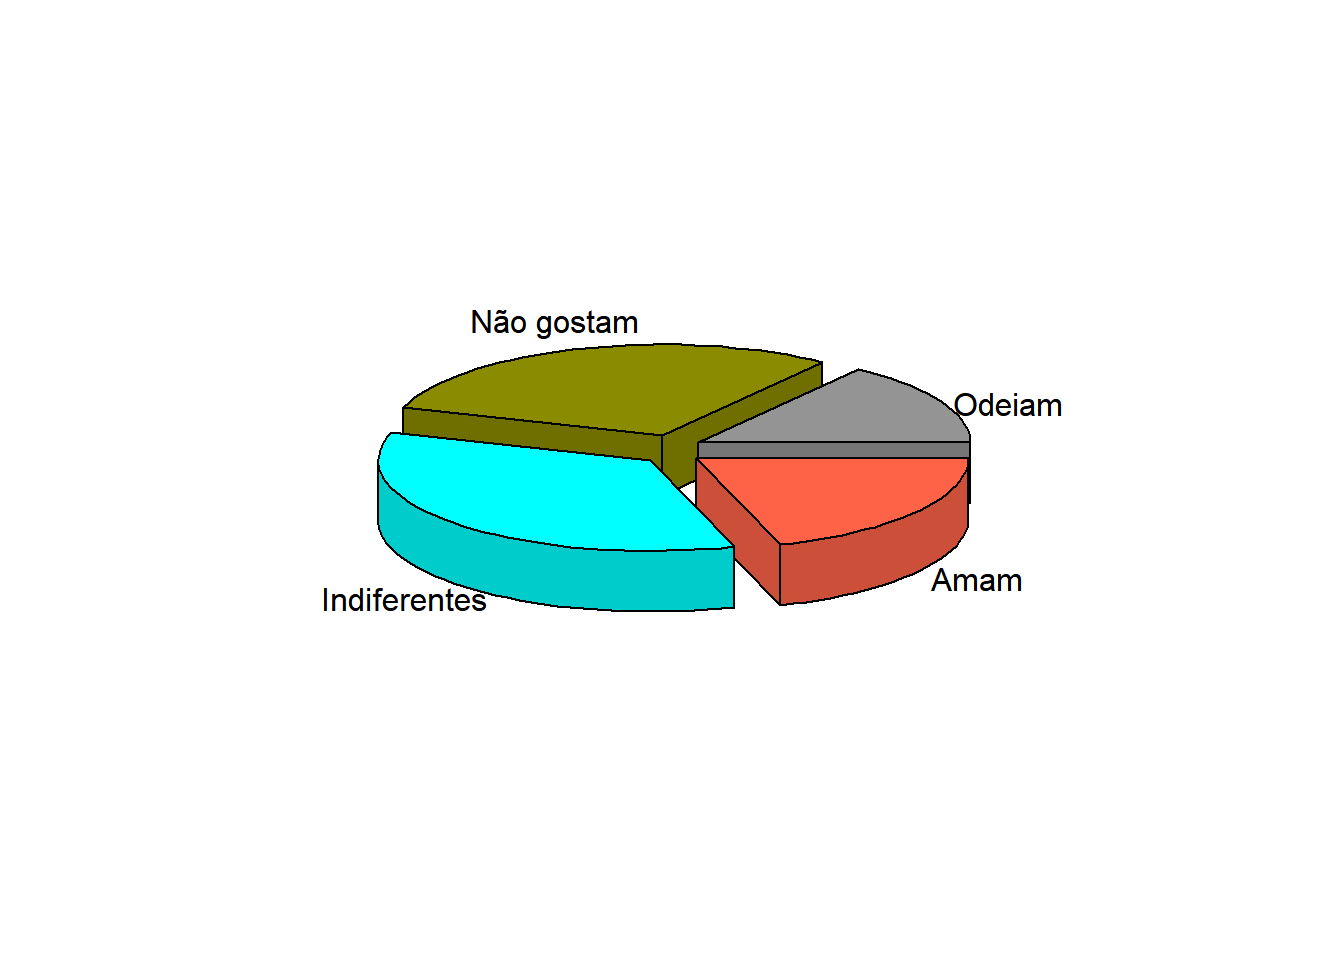
\includegraphics[width=1\linewidth,height=1\textheight]{bookdownproj_files/figure-latex/pie3d-1} 

}

\caption{Gráfico de Pizza: Opinião dos estudantes de Medicina.}\label{fig:pie3d}
\end{figure}

\subsection{Gráfico de barras}\label{gruxe1fico-de-barras}

Os gráficos de barra exibem a distribuição (frequências) de uma variável categórica através de barras verticais ou horizontais, ou sobrepostas \citep{kabacoff2011graphs}.

Assim como o gráfico de setores, o gráfico de barras é utilizado para representar a frequência absoluta ou percentual de diferentes categorias. As barras são proporcionais as frequências. A forma mais simples de solicitar um gráfico de barra no R é digitar a função \texttt{barplot()} do pacote básico. Esta função é específica para desenhar gráficos de barras horizontais e verticais e usa os seguintes argumentos:

\begin{itemize}
\tightlist
\item
  \emph{height} \(\longrightarrow\) um vetor ou matriz de valores que descreve as barras que constituem o gráfico;\\
\item
  \emph{width} \(\longrightarrow\) especifica largura das barras, com padrão de 1, opcional;\\
\item
  \emph{space} \(\longrightarrow\) a quantidade de espaço (como uma fração da largura média da barra) restante antes de cada barra. Pode ser fornecido como um único número ou um número por barra;\\
\item
  \emph{beside} \(\longrightarrow\) argumento lógico para especificar se colunas devem ser mostradas lado a lado;\\
\item
  \emph{col} \(\longrightarrow\) cores das barras componentes das barras, por padrão é usado \emph{grey} (cinza);\\
\item
  \emph{border} \(\longrightarrow\) cor das bordas das barras;\\
\item
  \emph{\ldots{}} \(\longrightarrow\) outros argumentos. Consulte a ajuda do R.
\end{itemize}

Para a construção do gráfico de barras simples da Figura \ref{fig:barra1}), foi utilizada a variável \texttt{categIdade}, anteriormente criada, a partir do conjunto de dados \texttt{dadosMater.xlsx}.

\begin{Shaded}
\begin{Highlighting}[]
\FunctionTok{barplot}\NormalTok{(}\FunctionTok{table}\NormalTok{(mater}\SpecialCharTok{$}\NormalTok{categIdade))}
\end{Highlighting}
\end{Shaded}

\begin{figure}[H]

{\centering 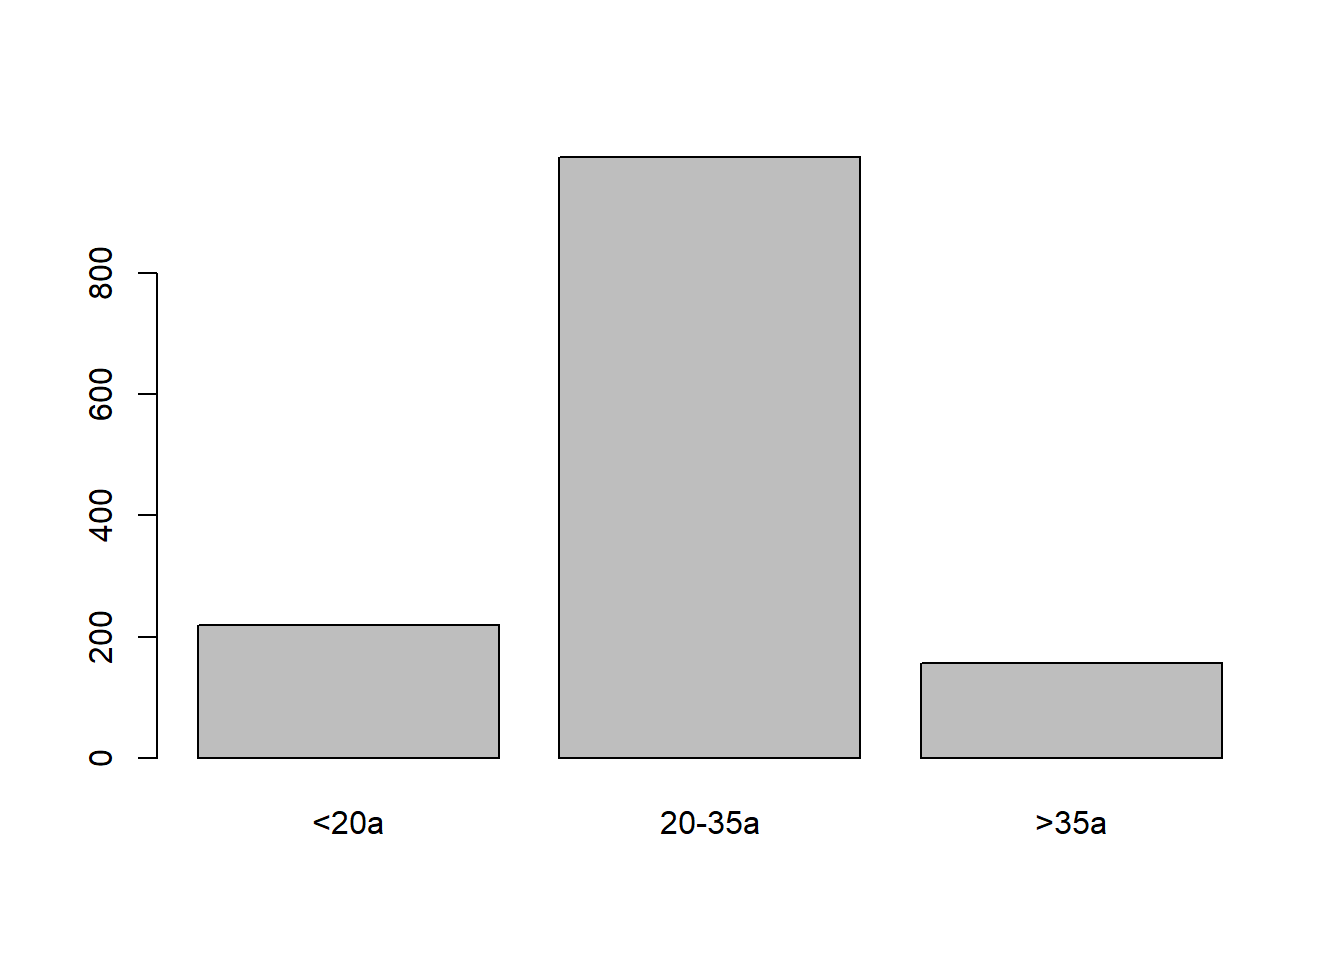
\includegraphics[width=0.8\linewidth,height=0.8\textheight]{bookdownproj_files/figure-latex/barra1-1} 

}

\caption{Gráfico de barra simples.}\label{fig:barra1}
\end{figure}

Observando a Figura \ref{fig:barra1}, verifica-se que não existem rótulos nos eixos \emph{x} e \emph{y} e o eixo \emph{y} tem um tamanho inferior a barra mais alta. Estes e outros problemas podem ser resolvidos modificando-se ou acrescentando outros argumentos na função \texttt{barplot()}. Existem vários argumentos e para conhece-los melhorpesquise no Help do RStudio. Em um gráfico de barra simples são suficientes as seguintes modificações que irão resultar na Figura \ref{fig:barra2}:

\begin{itemize}
\tightlist
\item
  Para corrigir a amplitude do eixo \emph{y}, existe o argumento \texttt{ylim\ =\ c(lim\ inf,\ lim\ sup)}. Na Tabela \ref{tab:tisch}, observa-se que a frequência máxima é de 992, assim estende-se até 1000, bem próximo da frequência da categoria, acrescentando \texttt{ylim\ =\ c\ (0,1000)}, separado por vírgulas de outros argumentos.
\item
  Para os rótulos se utiliza os argumentos \texttt{ylab\ =\ (“Frequência”)} e xlab = (``Faixa Etária''). Também, pode ser incluído um título no gráfico com o argumento m\texttt{ain\ =\ “Título”}. Observe que os títulos estão entre aspas.
\item
  Para modificar o tamanho das letras dos eixos \emph{x} e \emph{y}, que estão pouco visíveis, existe o argumento \texttt{cex.lab\ =\ 1}, que é o padrão. Para aumentar em 30\%, por exemplo, usar \texttt{cex.lab\ =\ 1.3}. Os nomes tem padrão \texttt{cex.names\ =\ 1,} para modificar pode-se usar 1.3, 1.5, etc. Se nada for modificado, o R imprime o padrão.
\item
  Para a cor das barras, use o argumento \texttt{col\ =\ (“cor”)}. Escolha a cor entre as 657 opções, ou deixe o padrão cinza (grey). O argumento \texttt{col.axis\ =\ “cor”} controla a cor dos valores dos eixos.
\item
  Para modificar a borda das barras que por padrão é preta, é possível mudar, usando o argumento \texttt{border\ =\ “cor”}. Sem borda basta colocar 0 (zero), no lugar da cor.
\item
  Para colocar as barras na posição horizontal, pode ser utilizado o argumento \texttt{horiz\ =\ TRUE}. Lembrar de inverter as barras. Ou seja, a variável x passa a ser y e vice-versa.
\item
  O argumento las = 1 faz o o texto do eixo \emph{y} ficar horizontal
\item
  A função \texttt{box(bty\ =\ "L")}, colocada após, e opcional, faz os eixos se encontraren em 0.
\end{itemize}

\begin{Shaded}
\begin{Highlighting}[]
\FunctionTok{barplot}\NormalTok{(}\FunctionTok{table}\NormalTok{(mater}\SpecialCharTok{$}\NormalTok{categIdade), }
        \AttributeTok{ylim =} \FunctionTok{c}\NormalTok{ (}\DecValTok{0}\NormalTok{,}\DecValTok{1000}\NormalTok{), }
        \AttributeTok{col=} \StringTok{"tomato"}\NormalTok{, }
        \AttributeTok{border =} \StringTok{"black"}\NormalTok{, }
        \AttributeTok{ylab=} \StringTok{"Frequência absoluta"}\NormalTok{, }
        \AttributeTok{xlab =} \StringTok{"Faixa etária"}\NormalTok{, }
        \AttributeTok{cex.lab =} \FloatTok{1.2}\NormalTok{,}
        \AttributeTok{las =} \DecValTok{1}\NormalTok{)}
\FunctionTok{box}\NormalTok{(}\AttributeTok{bty =} \StringTok{"L"}\NormalTok{)}
\end{Highlighting}
\end{Shaded}

\begin{figure}[H]

{\centering 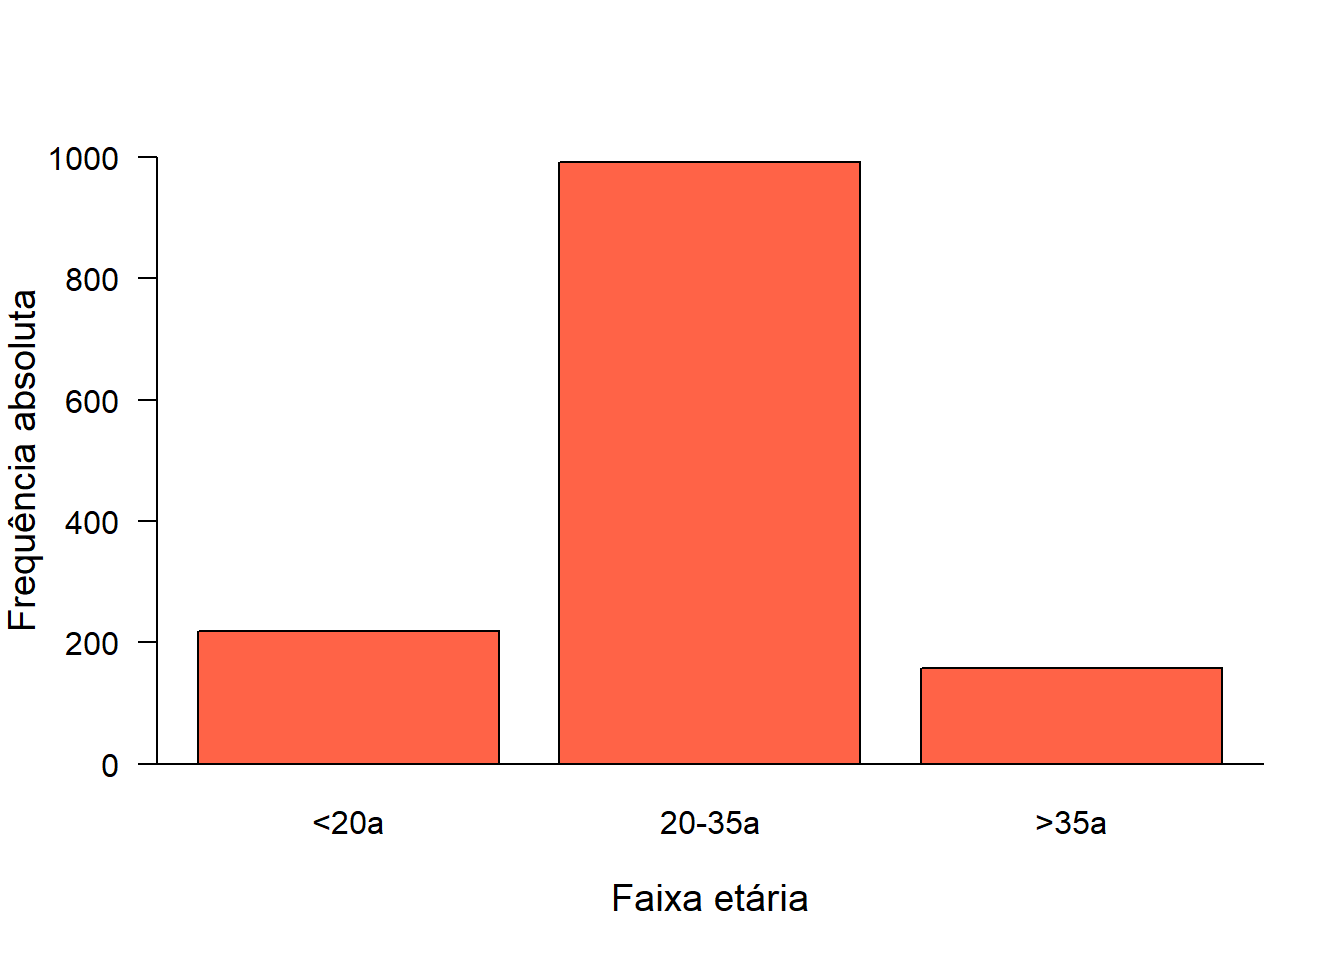
\includegraphics[width=0.8\linewidth,height=0.8\textheight]{bookdownproj_files/figure-latex/barra2-1} 

}

\caption{Gráfico de barra simples modificado.}\label{fig:barra2}
\end{figure}

Para que as barras fiquem horizontais como na Figura \ref{fig:barrah}, usa-se o argumento \texttt{horiz=TRUE}:

\begin{Shaded}
\begin{Highlighting}[]
\FunctionTok{barplot}\NormalTok{(}\FunctionTok{table}\NormalTok{(mater}\SpecialCharTok{$}\NormalTok{categIdade), }
        \AttributeTok{xlim =} \FunctionTok{c}\NormalTok{ (}\DecValTok{0}\NormalTok{,}\DecValTok{1000}\NormalTok{), }
        \AttributeTok{col=} \StringTok{"tomato"}\NormalTok{, }
        \AttributeTok{border =} \StringTok{"black"}\NormalTok{, }
        \AttributeTok{ylab=} \StringTok{"Faixa Etária"}\NormalTok{, }
        \AttributeTok{xlab =} \StringTok{"Frequência absoluta"}\NormalTok{, }
        \AttributeTok{cex.lab =} \FloatTok{1.2}\NormalTok{, }
        \AttributeTok{horiz=}\ConstantTok{TRUE}\NormalTok{)}
\FunctionTok{box}\NormalTok{(}\AttributeTok{bty =} \StringTok{"L"}\NormalTok{)}
\end{Highlighting}
\end{Shaded}

\begin{figure}[H]

{\centering 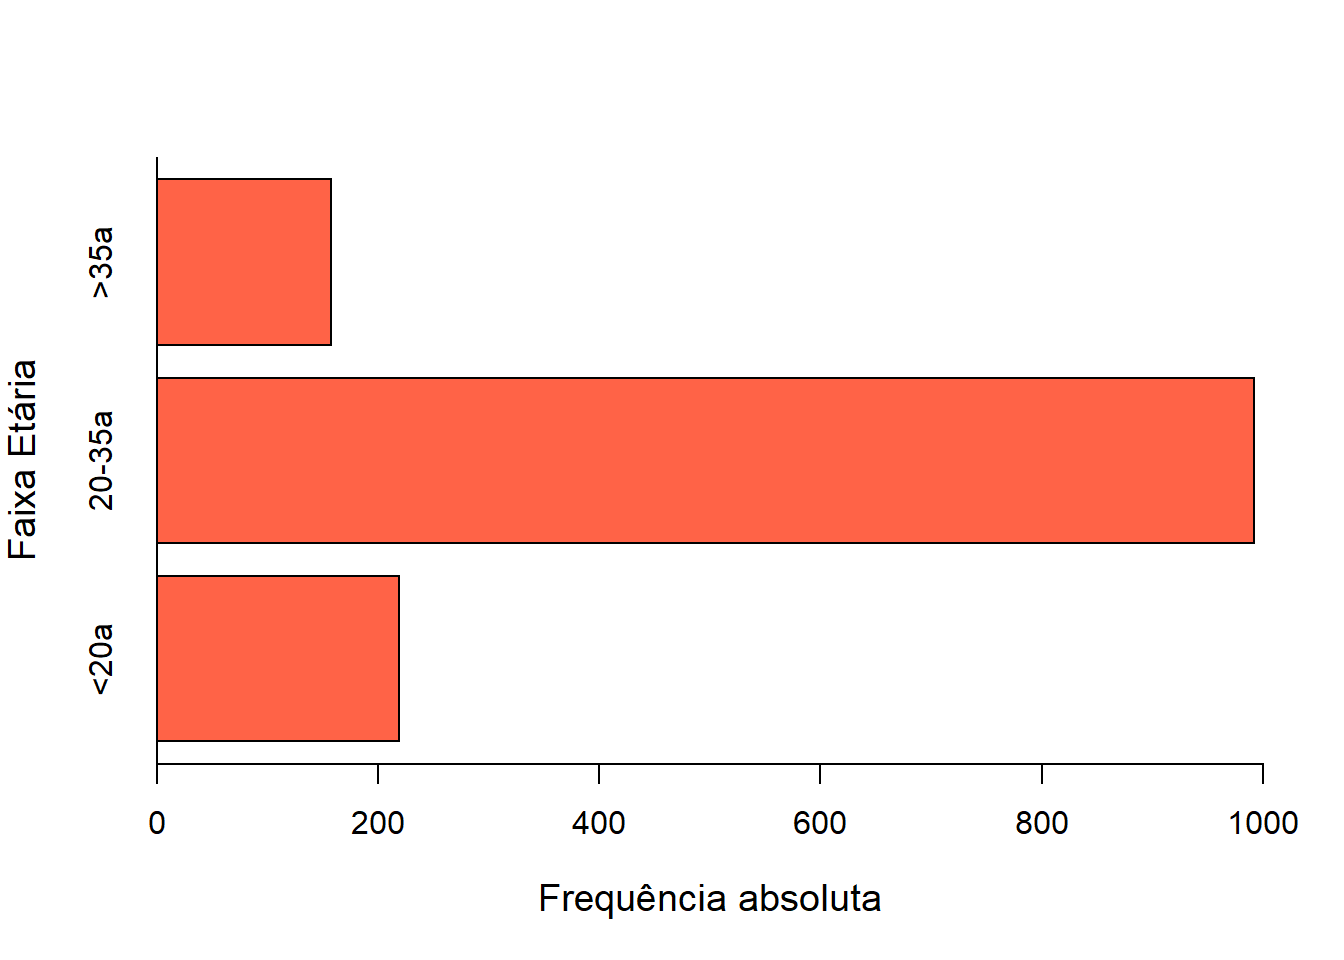
\includegraphics[width=0.8\linewidth,height=0.8\textheight]{bookdownproj_files/figure-latex/barrah-1} 

}

\caption{Gráfico com barras horizontais.}\label{fig:barrah}
\end{figure}

Além das modificações realizadas, é possível fazer outras para tornar o gráfico mais informativo . Por exemplo, pode-se colocar as frequência de cada barra no topo das mesmas (Figura \ref{fig:barra3}):

\begin{itemize}
\tightlist
\item
  \textbf{1º Passo}: Criar um gráfico de barras , colocando-o em um objeto \emph{x}, que conterá a coordenada X do centro de cada uma das barras. Para verificar isso, basta executar o objeto \emph{x};
\item
  \textbf{2º Passo}: colocar a tabela \texttt{table(mater\$idadeCateg)} com um objeto \emph{y} da classe matriz;
\item
  \textbf{3º Passo}: usar a funçãoo \texttt{text()} para colocar os valores.
\end{itemize}

\begin{Shaded}
\begin{Highlighting}[]
\NormalTok{x }\OtherTok{\textless{}{-}} \FunctionTok{barplot}\NormalTok{(}\FunctionTok{table}\NormalTok{(mater}\SpecialCharTok{$}\NormalTok{categIdade), }
             \AttributeTok{ylim =} \FunctionTok{c}\NormalTok{ (}\DecValTok{0}\NormalTok{,}\DecValTok{1000}\NormalTok{), }
             \AttributeTok{col=} \StringTok{"springgreen"}\NormalTok{, }
             \AttributeTok{border =} \StringTok{"black"}\NormalTok{, }
             \AttributeTok{ylab =} \StringTok{"Frequência absoluta"}\NormalTok{, }
             \AttributeTok{xlab =} \StringTok{"Faixa etária"}\NormalTok{, }
             \AttributeTok{cex.lab =} \FloatTok{1.2}\NormalTok{,}
             \AttributeTok{las =} \DecValTok{1}\NormalTok{)}
\FunctionTok{box}\NormalTok{(}\AttributeTok{bty =} \StringTok{"L"}\NormalTok{)}

\NormalTok{y }\OtherTok{\textless{}{-}} \FunctionTok{as.matrix}\NormalTok{(}\FunctionTok{table}\NormalTok{(mater}\SpecialCharTok{$}\NormalTok{categIdade))}

\FunctionTok{text}\NormalTok{ (x, y, }\AttributeTok{labels =} \FunctionTok{as.character}\NormalTok{(y), }\AttributeTok{adj =} \FunctionTok{c}\NormalTok{(}\FloatTok{0.5}\NormalTok{, }\DecValTok{2}\NormalTok{), }\AttributeTok{col =} \StringTok{"black"}\NormalTok{)}
\end{Highlighting}
\end{Shaded}

\begin{figure}[H]

{\centering 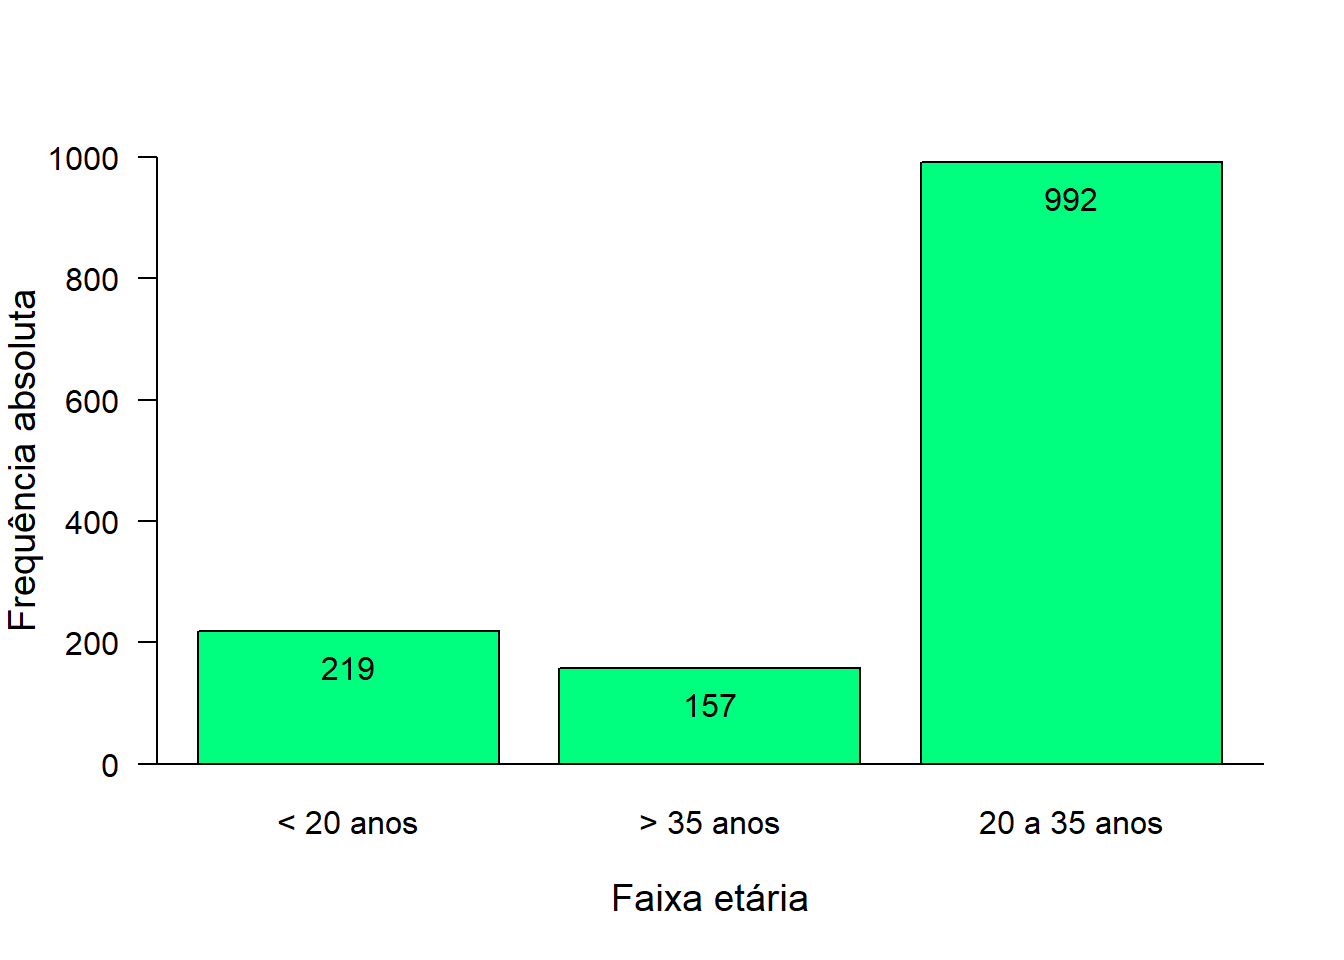
\includegraphics[width=0.8\linewidth,height=0.8\textheight]{bookdownproj_files/figure-latex/barra3-1} 

}

\caption{Gráfico de barra simples com frequências no topo.}\label{fig:barra3}
\end{figure}

\subsubsection{Gráfico de barras empilhadas}\label{gruxe1fico-de-barras-empilhadas}

Para este tipo de apresentação são utilizados, praticamente, os mesmos argumentos vistos para gerar um gráfico de barra simples. Como existem duas variáveis, há necessidade de avisar ao R como elas devem aparecer. Para isso, entra o argumento \texttt{beside\ =\ FALSE}, que informa que as barras não estarão uma ao lado da outra e sim empilhadas (Figura \ref{fig:stacked}). O padrão é as barras ficarem uma ao lado da outra.

Acrescenta-se uma legenda com a função \texttt{legend()} na parte superior esquerda (\texttt{topleft}). O argumento \texttt{bty\ =\ "n"} informa que será removido o quadro ao redor da legenda e \texttt{fill\ =\ c("dimgrey",\ "salmon")} são as cores das barras.

As duas variáveis a serem visualizadas são o \emph{hábito tabagista} entre as puérperas de acordo com a \emph{idade}. No conjunto de dados dadosMater.xlsx, o hábito tabagista está registrado na variável \texttt{fumo}, vista quando se estudou tabelas de contingência. Aqui se construirá uma tabela 3 x 2, \texttt{tabFumo2}:

\begin{Shaded}
\begin{Highlighting}[]
\NormalTok{tabFumo2 }\OtherTok{\textless{}{-}} \FunctionTok{table}\NormalTok{(mater}\SpecialCharTok{$}\NormalTok{fumo, mater}\SpecialCharTok{$}\NormalTok{categIdade)}

\FunctionTok{barplot}\NormalTok{(tabFumo2,}
        \AttributeTok{beside =} \ConstantTok{FALSE}\NormalTok{,}
        \AttributeTok{ylim =} \FunctionTok{c}\NormalTok{(}\DecValTok{0}\NormalTok{, }\DecValTok{1000}\NormalTok{),}
        \AttributeTok{xlab=}\StringTok{"Faixa Etária"}\NormalTok{, }
        \AttributeTok{ylab =} \StringTok{"Frequência"}\NormalTok{, }
        \AttributeTok{col =} \FunctionTok{c}\NormalTok{ (}\StringTok{"dimgrey"}\NormalTok{, }\StringTok{"cadetblue1"}\NormalTok{),  }
        \AttributeTok{cex.lab =} \DecValTok{1}\NormalTok{, }
        \AttributeTok{cex.axis =} \DecValTok{1}\NormalTok{, }
        \AttributeTok{cex.names =} \DecValTok{1}\NormalTok{,}
        \AttributeTok{las =} \DecValTok{1}\NormalTok{)}
\FunctionTok{box}\NormalTok{(}\AttributeTok{bty =} \StringTok{"L"}\NormalTok{)}
\FunctionTok{legend}\NormalTok{ (}\StringTok{"topleft"}\NormalTok{,}
        \AttributeTok{legend =} \FunctionTok{c}\NormalTok{(}\StringTok{"Fumantes"}\NormalTok{, }\StringTok{"Não Fumantes"}\NormalTok{), }
        \AttributeTok{fill =} \FunctionTok{c}\NormalTok{(}\StringTok{"dimgrey"}\NormalTok{, }\StringTok{"cadetblue1"}\NormalTok{), }
        \AttributeTok{bty=}\StringTok{"n"}\NormalTok{, }
        \AttributeTok{cex =} \DecValTok{1}\NormalTok{)}
\end{Highlighting}
\end{Shaded}

\begin{figure}[H]

{\centering 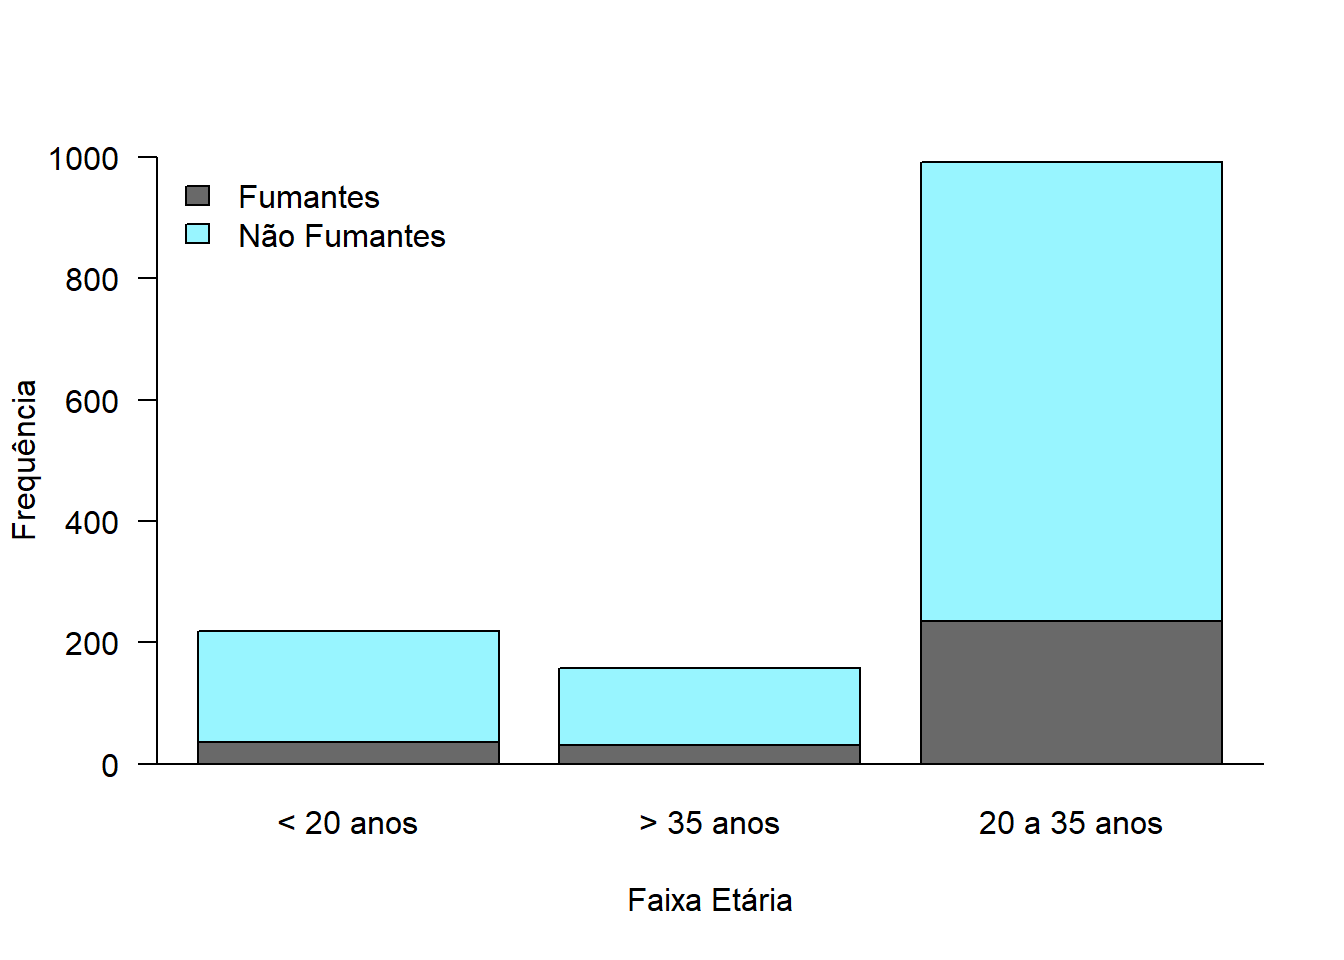
\includegraphics[width=0.9\linewidth,height=0.9\textheight]{bookdownproj_files/figure-latex/stacked-1} 

}

\caption{Gráfico de barras empilhadas.}\label{fig:stacked}
\end{figure}

\subsubsection{Gráfico de barras lado a lado}\label{gruxe1fico-de-barras-lado-a-lado}

É igual a anterior, apenas com o argumento \texttt{beside\ =\ TRUE} (Figura \ref{fig:side}).

\begin{Shaded}
\begin{Highlighting}[]
\FunctionTok{barplot}\NormalTok{(tabFumo2,}
        \AttributeTok{beside =} \ConstantTok{TRUE}\NormalTok{,}
        \AttributeTok{ylim =} \FunctionTok{c}\NormalTok{(}\DecValTok{0}\NormalTok{, }\DecValTok{1000}\NormalTok{),}
        \AttributeTok{xlab=}\StringTok{"Faixa Etária"}\NormalTok{, }
        \AttributeTok{ylab =} \StringTok{"Frequência"}\NormalTok{, }
        \AttributeTok{col =} \FunctionTok{c}\NormalTok{ (}\StringTok{"dimgrey"}\NormalTok{, }\StringTok{"cadetblue1"}\NormalTok{),  }
        \AttributeTok{cex.lab =} \DecValTok{1}\NormalTok{, }
        \AttributeTok{cex.axis =} \DecValTok{1}\NormalTok{, }
        \AttributeTok{cex.names =} \DecValTok{1}\NormalTok{,}
        \AttributeTok{las =} \DecValTok{1}\NormalTok{)}
\FunctionTok{box}\NormalTok{(}\AttributeTok{bty =} \StringTok{"L"}\NormalTok{)}
\FunctionTok{legend}\NormalTok{ (}\StringTok{"topleft"}\NormalTok{,}
        \AttributeTok{legend =} \FunctionTok{c}\NormalTok{(}\StringTok{"Fumantes"}\NormalTok{, }\StringTok{"Não Fumantes"}\NormalTok{), }
        \AttributeTok{fill =} \FunctionTok{c}\NormalTok{(}\StringTok{"dimgrey"}\NormalTok{, }\StringTok{"cadetblue1"}\NormalTok{), }
        \AttributeTok{bty=}\StringTok{"n"}\NormalTok{, }
        \AttributeTok{cex =} \DecValTok{1}\NormalTok{)}
\end{Highlighting}
\end{Shaded}

\begin{figure}[H]

{\centering 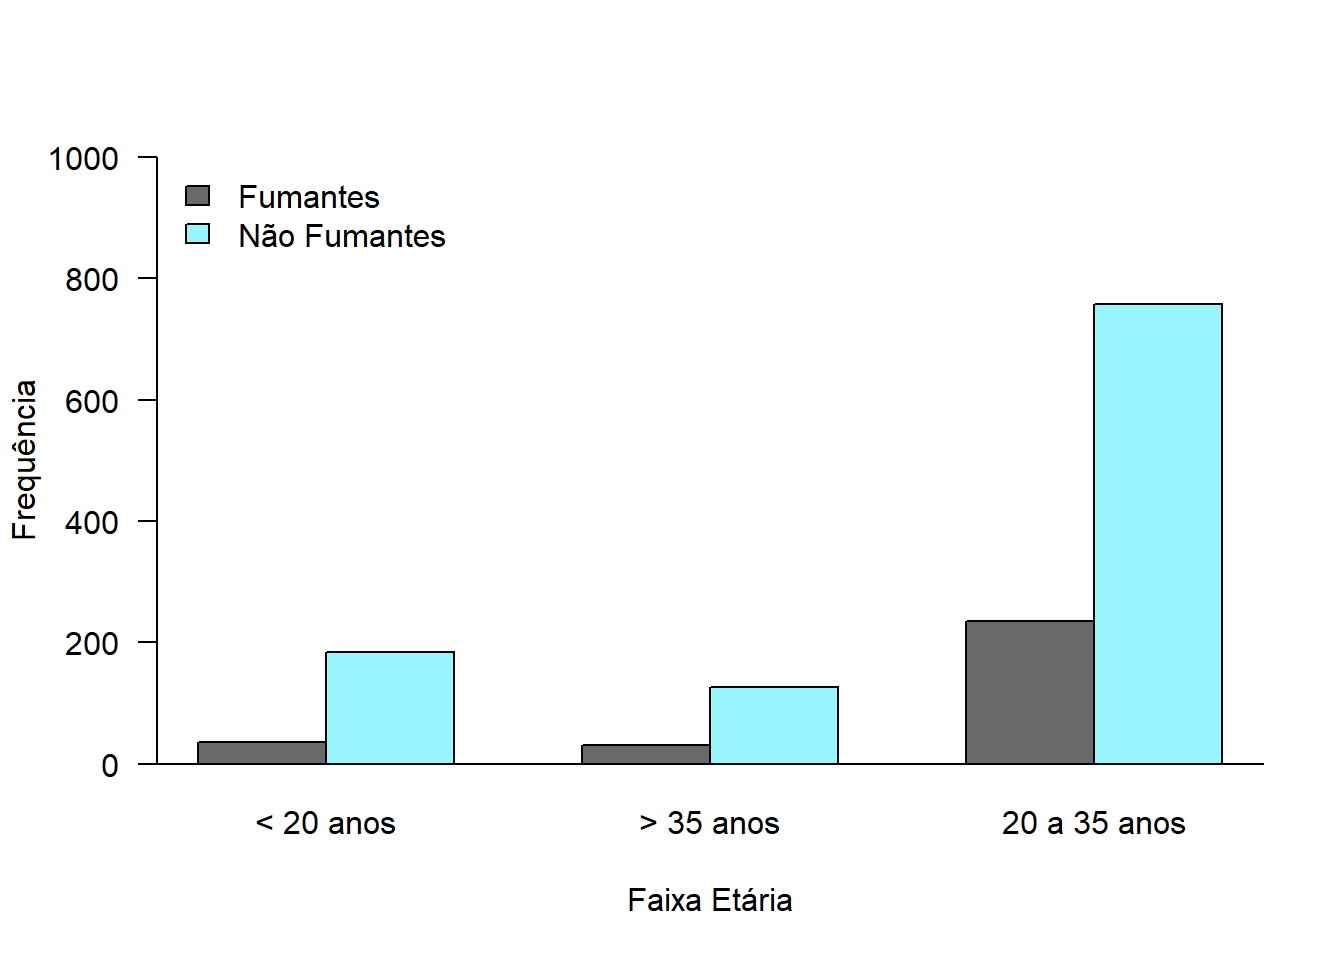
\includegraphics[width=0.9\linewidth,height=0.9\textheight]{bookdownproj_files/figure-latex/side-1} 

}

\caption{Gráfico de barras lado a lado}\label{fig:side}
\end{figure}

\subsubsection{Gráfico de barras para uma variável discreta}\label{gruxe1fico-de-barras-para-uma-variuxe1vel-discreta}

A variável \texttt{mater\$para}, número de filhos anteriores ao atual, é uma variável numérica discreta e, para representá-la, o mais adequado é usar um gráfico de barras simples Figura \ref{fig:discreta}).

\begin{Shaded}
\begin{Highlighting}[]
\NormalTok{tab\_filhos}\OtherTok{\textless{}{-}} \FunctionTok{table}\NormalTok{ (mater}\SpecialCharTok{$}\NormalTok{para) }

\FunctionTok{barplot}\NormalTok{ (tab\_filhos, }
         \AttributeTok{col =} \StringTok{"tomato"}\NormalTok{, }
         \AttributeTok{xlab=}\StringTok{"Número de filhos anteriores ao atual"}\NormalTok{, }
         \AttributeTok{ylab =} \StringTok{"Frequência"}\NormalTok{,}
         \AttributeTok{ylim =} \FunctionTok{c}\NormalTok{(}\DecValTok{0}\NormalTok{, }\DecValTok{500}\NormalTok{),}
         \AttributeTok{cex.lab =} \DecValTok{1}\NormalTok{, }
         \AttributeTok{cex.axis =} \DecValTok{1}\NormalTok{, }
         \AttributeTok{cex.names =} \DecValTok{1}\NormalTok{,}
         \AttributeTok{las =} \DecValTok{1}\NormalTok{)}
\FunctionTok{box}\NormalTok{(}\AttributeTok{bty =} \StringTok{"L"}\NormalTok{)}
\end{Highlighting}
\end{Shaded}

\begin{figure}[H]

{\centering 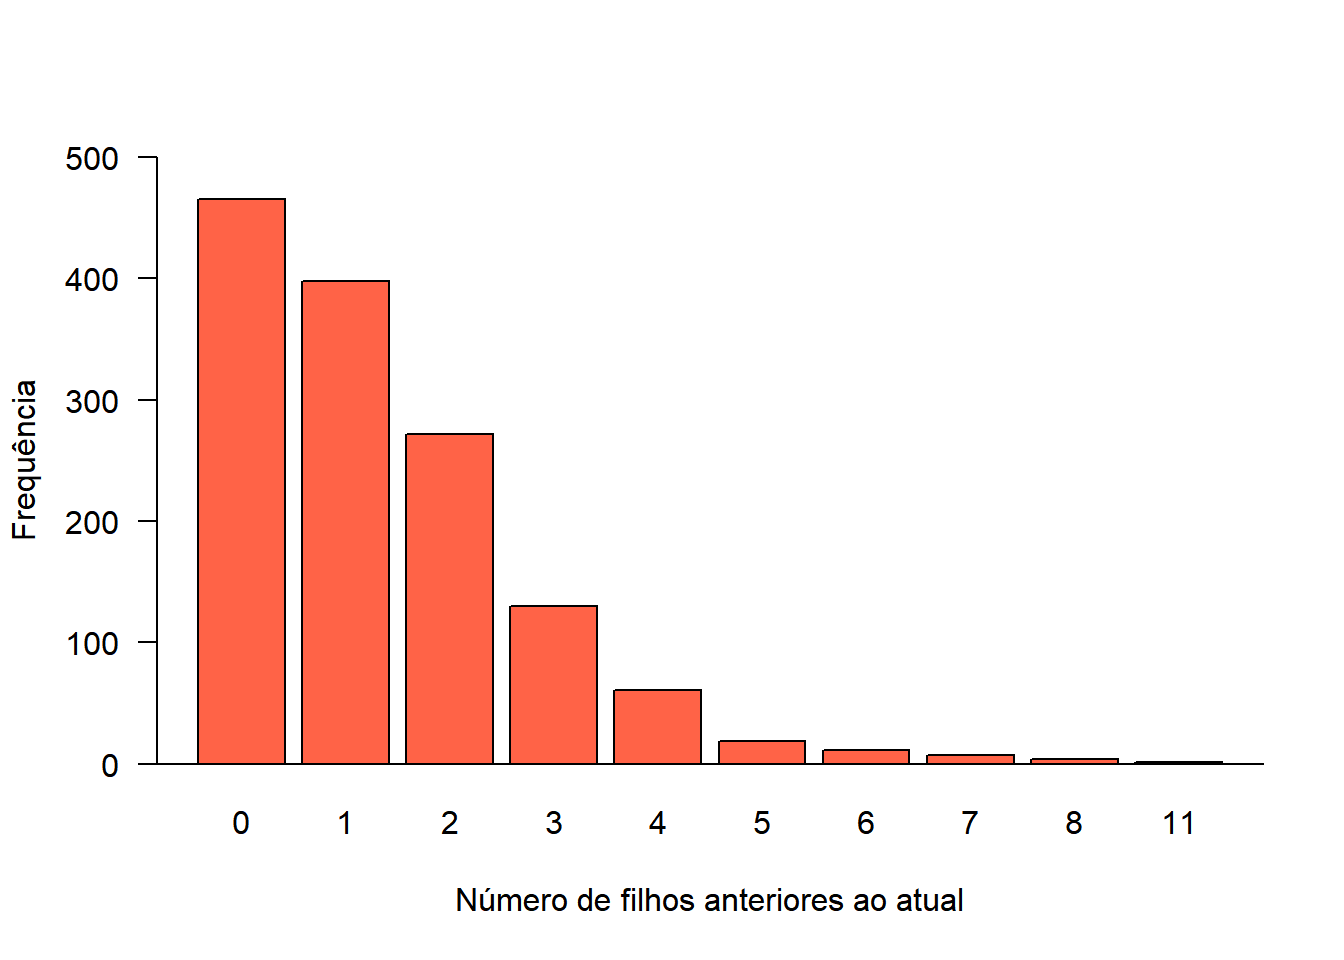
\includegraphics[width=0.8\linewidth,height=0.8\textheight]{bookdownproj_files/figure-latex/discreta-1} 

}

\caption{Gráfico de barras para uma variável discreta}\label{fig:discreta}
\end{figure}

\subsection{Gráfico de barra de erro}\label{gruxe1fico-de-barra-de-erro}

O \emph{gráfico de barra de erro} é um tipo de gráfico barra acrescido de uma medida de dispersão: desvio padrão, intervalos de confiança ou erro padrão. As barras de erro dão uma ideia geral de quão precisa é uma medição ou, inversamente, quão longe o valor observado está do valor verdadeiro.

Continuando a usar o arquivo \texttt{dadosMater.xlsx}, será selecionada uma amostra de recém-nascidos a termo, definido pela OMS como o nascido de 37 semanas completas a 42 semanas incompletas (259 a 293 dias). A partir destes dados, será construido um gráfico de barra de erro dos recém-nascidos do sexo masculino e feminino.

Inicialmente, deve ser instalado e carregado o pacote \texttt{Hmisc} \citet{harrell2022hmisc}, necessário para fornecer a função \texttt{errbar()} que irá construir o gráfico de de barra de erro.

A seguir, serão filtrados do conjunto de dados em uso, \texttt{mater}, os recém-nascidos a termo. O conjunto resultante será atribuído a um objeto denominado \texttt{rnt} e , usando o operador pipe \%\textgreater\% será usada a função \texttt{summarise()} e \texttt{group\_by()} provenientes do pacote \texttt{dplyr}, para calcular as medidas resumidoras, de acordo com o sexo. Como a variável \texttt{sexo} encontra-se como numérica, será transformada em fator:

\begin{Shaded}
\begin{Highlighting}[]
\NormalTok{mater}\SpecialCharTok{$}\NormalTok{sexo }\OtherTok{\textless{}{-}} \FunctionTok{factor}\NormalTok{(mater}\SpecialCharTok{$}\NormalTok{sexo,}
                      \AttributeTok{labels =} \FunctionTok{c}\NormalTok{(}\StringTok{\textquotesingle{}masc\textquotesingle{}}\NormalTok{, }\StringTok{\textquotesingle{}fem\textquotesingle{}}\NormalTok{))}
 
\NormalTok{ rnt }\OtherTok{\textless{}{-}}\NormalTok{ mater }\SpecialCharTok{\%\textgreater{}\%} 
   \FunctionTok{filter}\NormalTok{(ig }\SpecialCharTok{\textgreater{}=} \DecValTok{37} \SpecialCharTok{\&}\NormalTok{ ig }\SpecialCharTok{\textless{}} \DecValTok{42}\NormalTok{) }\SpecialCharTok{\%\textgreater{}\%} 
   \FunctionTok{group\_by}\NormalTok{(sexo) }\SpecialCharTok{\%\textgreater{}\%} 
   \FunctionTok{summarise}\NormalTok{(}\AttributeTok{n =} \FunctionTok{n}\NormalTok{(),}
             \AttributeTok{media =} \FunctionTok{mean}\NormalTok{(pesoRN, }\AttributeTok{na.rm =}\NormalTok{ T),}
             \AttributeTok{dp =} \FunctionTok{sd}\NormalTok{(pesoRN, }\AttributeTok{na.rm =}\NormalTok{ T),}
             \AttributeTok{l\_inf =}\NormalTok{ media }\SpecialCharTok{{-}} \FloatTok{1.96}\SpecialCharTok{*}\NormalTok{dp,}
             \AttributeTok{l\_sup =}\NormalTok{ media }\SpecialCharTok{+} \FloatTok{1.96}\SpecialCharTok{*}\NormalTok{dp)}

\NormalTok{ rnt}
\end{Highlighting}
\end{Shaded}

\begin{verbatim}
## # A tibble: 2 x 6
##   sexo      n media    dp l_inf l_sup
##   <fct> <int> <dbl> <dbl> <dbl> <dbl>
## 1 masc    592 3274.  458. 2376. 4172.
## 2 fem     493 3147.  458. 2250. 4044.
\end{verbatim}

O próximo passo é criar um objeto, denominado \texttt{barras}, que irá receber as médias dos pesos dos recém-nascidos masculinos e femininos, que representam a altura das barras. Este objeta servirá de base para a construção de um gráfico de barras que será recebido por outro objeto, \texttt{bp}.
Finalmente, coloca-se os limites inferiores e superiores para cada sexo, usando os valores calculados pela função summarise() que junto com o objeto bp constituem-se de argumentos da função \texttt{errbar()} (Figura \ref{fig:errorbar}). Veja maiores detalhes na ajuda do R (\texttt{?errbar}).

\begin{Shaded}
\begin{Highlighting}[]
\NormalTok{barras }\OtherTok{\textless{}{-}} \FunctionTok{c}\NormalTok{(rnt}\SpecialCharTok{$}\NormalTok{media[}\DecValTok{1}\NormalTok{], rnt}\SpecialCharTok{$}\NormalTok{media[}\DecValTok{2}\NormalTok{])}

\NormalTok{ bp }\OtherTok{\textless{}{-}} \FunctionTok{barplot}\NormalTok{(barras,}
               \AttributeTok{ylim=}\FunctionTok{c}\NormalTok{(}\DecValTok{0}\NormalTok{,}\DecValTok{4200}\NormalTok{), }
               \AttributeTok{ylab =} \StringTok{"Peso do Recém{-}nascido (g)"}\NormalTok{,}
               \AttributeTok{cex.lab =} \FloatTok{1.2}\NormalTok{,}
               \AttributeTok{cex.axis =} \FloatTok{0.8}\NormalTok{,}
               \AttributeTok{cex.names =} \DecValTok{1}\NormalTok{,}
               \AttributeTok{space =} \FunctionTok{c}\NormalTok{(}\DecValTok{0}\NormalTok{,}\FloatTok{0.5}\NormalTok{),}
               \AttributeTok{names.arg=}\FunctionTok{c}\NormalTok{(}\StringTok{"Meninos"}\NormalTok{, }\StringTok{"Meninas"}\NormalTok{), }
               \AttributeTok{col =} \FunctionTok{c}\NormalTok{(}\StringTok{"lightblue"}\NormalTok{, }\StringTok{" pink2"}\NormalTok{),}
               \AttributeTok{las =} \DecValTok{1}\NormalTok{)}
 \FunctionTok{box}\NormalTok{(}\AttributeTok{bty =} \StringTok{"L"}\NormalTok{)}

\NormalTok{ lim\_inf }\OtherTok{\textless{}{-}} \FunctionTok{c}\NormalTok{(rnt}\SpecialCharTok{$}\NormalTok{l\_inf[}\DecValTok{1}\NormalTok{], rnt}\SpecialCharTok{$}\NormalTok{l\_inf[}\DecValTok{2}\NormalTok{])}
\NormalTok{ lim\_sup }\OtherTok{\textless{}{-}} \FunctionTok{c}\NormalTok{(rnt}\SpecialCharTok{$}\NormalTok{l\_sup[}\DecValTok{1}\NormalTok{], rnt}\SpecialCharTok{$}\NormalTok{l\_sup[}\DecValTok{2}\NormalTok{])}

 \FunctionTok{errbar}\NormalTok{(bp, barras, lim\_inf, lim\_sup, }\AttributeTok{add =} \ConstantTok{TRUE}\NormalTok{, }\AttributeTok{xlab =} \ConstantTok{NULL}\NormalTok{)}
\end{Highlighting}
\end{Shaded}

\begin{figure}[H]

{\centering 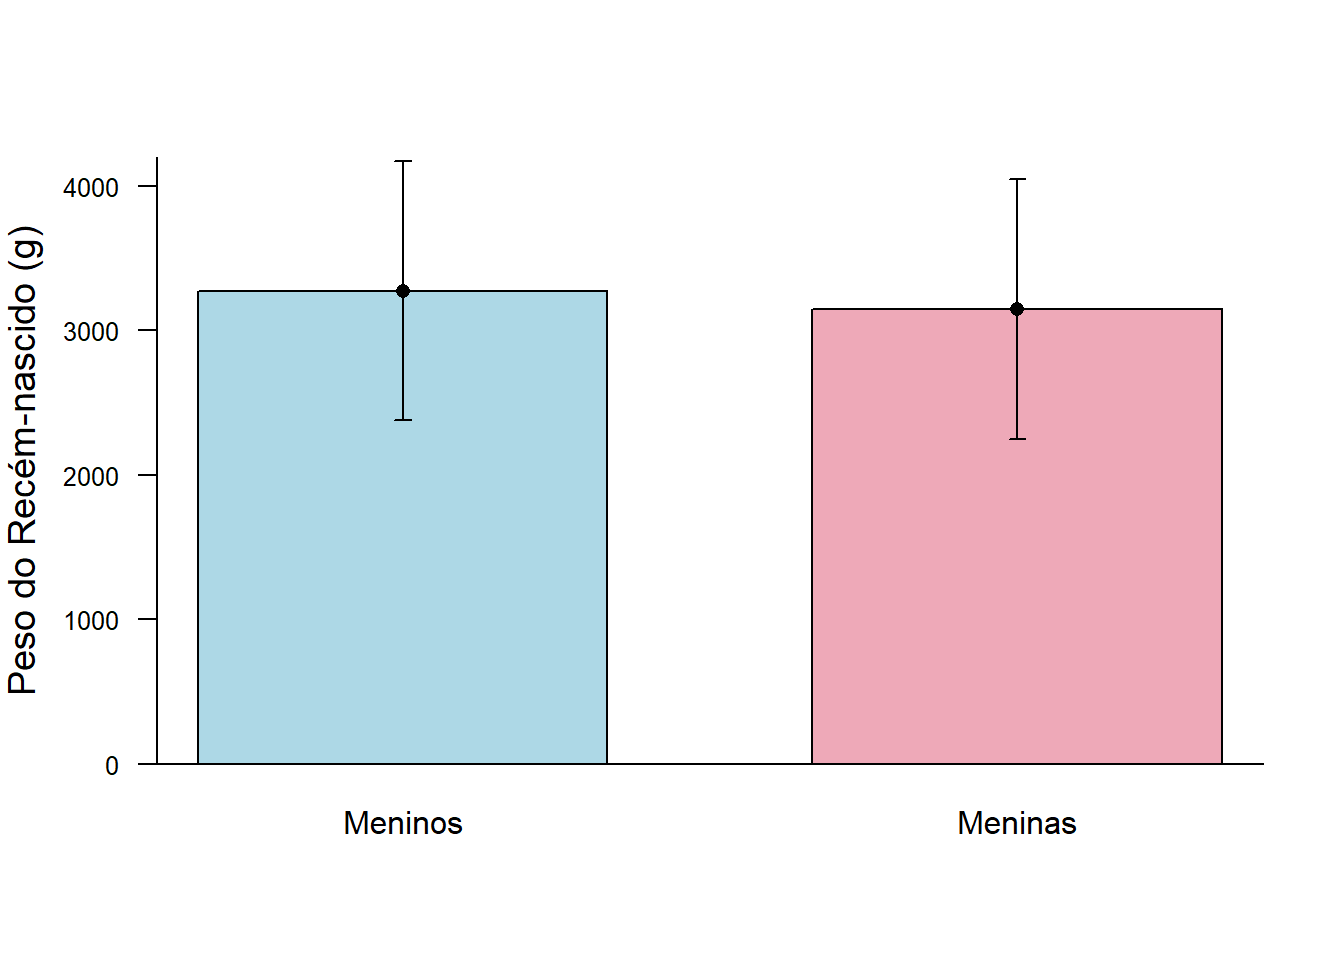
\includegraphics[width=0.8\linewidth,height=0.8\textheight]{bookdownproj_files/figure-latex/errorbar-1} 

}

\caption{Gráfico de barras de erro}\label{fig:errorbar}
\end{figure}

\subsection{Histograma}\label{histograma}

O \emph{histograma} é uma ferramenta gráfica que fornece informações sobre o formato da distribuição e dispersão dos dados, permitindo verificar se existe ou não simetria. É usado para dados contínuos.

No histograma, as frequências observadas são representadas por intervalos de classes de ocorrência que estão no eixo \emph{x} e a altura das barras, representando a frequência de cada intervalo, no eixo \emph{y}. A área de cada barra é proporcional à porcentagem de observações de cada intervalo.

O R base possui uma função, denominada de \texttt{hist()} que constroi o histograma e possui vários argumentos:

\begin{itemize}
\tightlist
\item
  \emph{x} \(\longrightarrow\) um vetor numérico usado na construção do histograma\\
\item
  \emph{breaks} \(\longrightarrow\) especifica o número de barras
\item
  \emph{freq} \(\longrightarrow\) lógico; se \texttt{TRUE} (padrão), o histograma é uma representação de frequências; se \texttt{FALSE}, densidades de probabilidade, densidade de componentes, são plotados
\item
  \emph{col} \(\longrightarrow\) cor a ser usada para preencher as barras. O padrão de NULL produz barras não preenchidas
\item
  \emph{border} \(\longrightarrow\) cor da borda ao redor das barras. O padrão é usar a cor de primeiro plano padrão
\item
  \emph{main, xlab, ylab} \(\longrightarrow\) rótulo do título, do eixo \emph{x} e do eixo \emph{y}. Para remover o rótulousar \texttt{NULL.}
\item
  \emph{xlim, ylim} \(\longrightarrow\) limites do eixo \emph{x} e do eixo \emph{y}.
\end{itemize}

\subsubsection{Histograma Simples}\label{histograma-simples}

Será usada a variável altura, proveniente da arquivo mater (veja início da seção), para a construção do histograma, executando:.

\begin{Shaded}
\begin{Highlighting}[]
\FunctionTok{hist}\NormalTok{(mater}\SpecialCharTok{$}\NormalTok{altura)}
\end{Highlighting}
\end{Shaded}

\begin{figure}[H]

{\centering 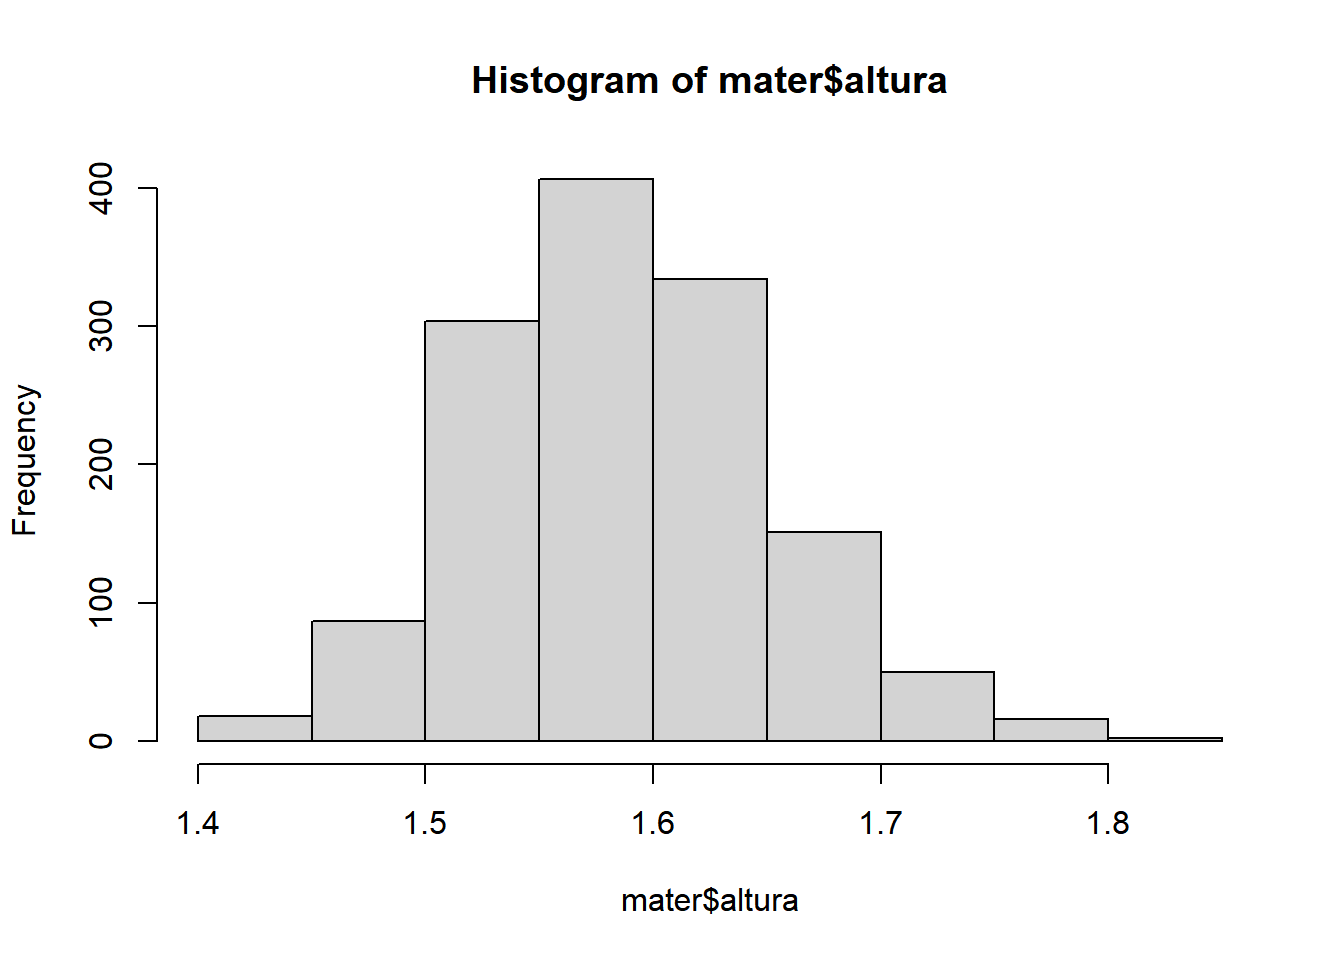
\includegraphics[width=0.8\linewidth,height=0.8\textheight]{bookdownproj_files/figure-latex/histb-1} 

}

\caption{Histograma básico}\label{fig:histb}
\end{figure}

No histograma da Figura \ref{fig:histb}, observam-se alguns problemas que devem ser melhorados para tornar a sua aparência mais elegante.

\begin{itemize}
\tightlist
\item
  O rótulo dos eixo \emph{x} está com o nome da variável e do eixo \emph{y} está em inglês;
\item
  O título do histograma está em inglês e repete o eixo \emph{x}. Pode ser removido.
\item
  O eixo \emph{y} tem um limite superior menor do que a barra mais alta;
\item
  O gráfico está na cor cinza, que conforme o interesse pode ser modificada;
\item
  O número de barras pode ser modificado com o argumento \texttt{breaks}. Existe uma função no R que permite calcular o número de intervalos, usando a \emph{regra de Sturges} (\texttt{nclass.Sturges()}). Entretanto, na maioria das vezes, é o objetivo do estudo quem determina o número de barras e, também, porque nem sempre o R obedece ao argumento.
\end{itemize}

É importante saber o limite inferior e superior da variável, para construir o eixo \emph{x}. Pode-se fazer isso, com as funções \texttt{min()} e \texttt{max()}:

\begin{Shaded}
\begin{Highlighting}[]
\FunctionTok{min}\NormalTok{(mater}\SpecialCharTok{$}\NormalTok{altura, }\AttributeTok{na.rm =} \ConstantTok{TRUE}\NormalTok{)}
\end{Highlighting}
\end{Shaded}

\begin{verbatim}
## [1] 1.4
\end{verbatim}

\begin{Shaded}
\begin{Highlighting}[]
\FunctionTok{max}\NormalTok{(mater}\SpecialCharTok{$}\NormalTok{altura, }\AttributeTok{na.rm =} \ConstantTok{TRUE}\NormalTok{)}
\end{Highlighting}
\end{Shaded}

\begin{verbatim}
## [1] 1.85
\end{verbatim}

O número de classes é igual a:

\begin{Shaded}
\begin{Highlighting}[]
\FunctionTok{nclass.Sturges}\NormalTok{(mater}\SpecialCharTok{$}\NormalTok{altura)}
\end{Highlighting}
\end{Shaded}

\begin{verbatim}
## [1] 12
\end{verbatim}

Acrescentado argumentos, modifica-se o aspecto do histograma (Figura \ref{fig:histmod}):

\begin{Shaded}
\begin{Highlighting}[]
\FunctionTok{hist}\NormalTok{(mater}\SpecialCharTok{$}\NormalTok{altura,}
     \AttributeTok{breaks =} \DecValTok{12}\NormalTok{,}
     \AttributeTok{ylim =} \FunctionTok{c}\NormalTok{ (}\DecValTok{0}\NormalTok{, }\DecValTok{450}\NormalTok{),}
     \AttributeTok{xlim =} \FunctionTok{c}\NormalTok{ (}\FloatTok{1.4}\NormalTok{, }\FloatTok{1.9}\NormalTok{),}
     \AttributeTok{main=} \ConstantTok{NULL}\NormalTok{, }
     \AttributeTok{ylab =} \StringTok{"Frequência"}\NormalTok{, }
     \AttributeTok{xlab =} \StringTok{"Altura da gestante (metros)"}\NormalTok{,}
     \AttributeTok{col =} \StringTok{"tomato"}\NormalTok{,}
     \AttributeTok{las =} \DecValTok{1}\NormalTok{)}
\FunctionTok{box}\NormalTok{(}\AttributeTok{bty =} \StringTok{"L"}\NormalTok{)}
\end{Highlighting}
\end{Shaded}

\begin{figure}[H]

{\centering 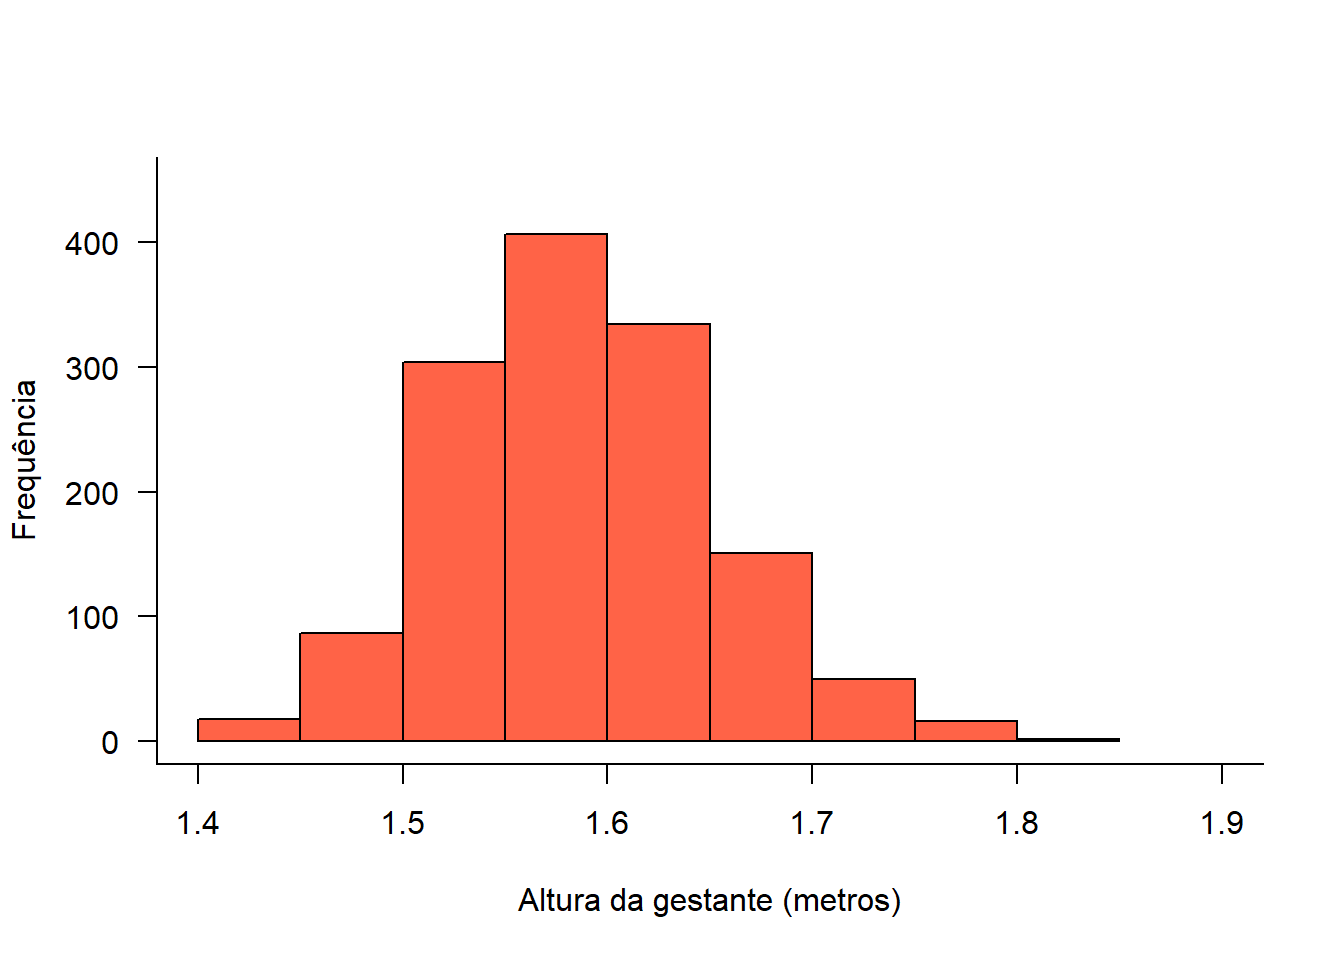
\includegraphics[width=0.8\linewidth,height=0.8\textheight]{bookdownproj_files/figure-latex/histmod-1} 

}

\caption{Histograma modificado}\label{fig:histmod}
\end{figure}

Observe que o formato do histograma é igual ao anterior, mudando a cor das barras, o limite do eixo \emph{y} e os rótulos dos eixos. O R não modificou o número de barras. Ou seja, não obedeceu à modificação do argumento breaks = 12. Ele escolheu o que achou mais adequado!

\subsubsection{Histograma com curva normal sobreposta}\label{histograma-com-curva-normal-sobreposta}

Eventualmente, para melhor comparar a distribuição dos dados, usamos uma curva normal sobreposta que servirá de indicador (Figura \ref{fig:histnormal}). A distribuição normal será discutida mais adiante (Capítulo 7).

\begin{enumerate}
\def\labelenumi{\arabic{enumi})}
\item
  Construir um histograma de densidade, que é a proporção de todas as observações que se enquadram dentro do intervalo. Na função \texttt{hist()}, modificar o argumento para \texttt{freq\ =\ FALSE}.
\item
  Adicionar uma curva normal ao histograma, usando a função \texttt{curve()}. Calcular antes a média e o desvio padrão da variável \texttt{mater\$altura}.
\end{enumerate}

\begin{Shaded}
\begin{Highlighting}[]
\NormalTok{mu }\OtherTok{\textless{}{-}} \FunctionTok{mean}\NormalTok{(mater}\SpecialCharTok{$}\NormalTok{altura, }\AttributeTok{na.rm =}\ConstantTok{TRUE}\NormalTok{)}
\NormalTok{dp }\OtherTok{\textless{}{-}} \FunctionTok{sd}\NormalTok{(mater}\SpecialCharTok{$}\NormalTok{altura, }\AttributeTok{na.rm =} \ConstantTok{TRUE}\NormalTok{)}

\FunctionTok{hist}\NormalTok{(mater}\SpecialCharTok{$}\NormalTok{altura,}
     \AttributeTok{ylim =} \FunctionTok{c}\NormalTok{ (}\DecValTok{0}\NormalTok{, }\DecValTok{6}\NormalTok{),}
     \AttributeTok{xlim =} \FunctionTok{c}\NormalTok{ (}\FloatTok{1.4}\NormalTok{, }\FloatTok{1.9}\NormalTok{),}
     \AttributeTok{main=} \ConstantTok{NULL}\NormalTok{, }
     \AttributeTok{ylab =} \StringTok{"Densidade"}\NormalTok{, }
     \AttributeTok{xlab =} \StringTok{"Altura da gestante (metros)"}\NormalTok{,}
     \AttributeTok{col =}\StringTok{"steelblue"}\NormalTok{,}
     \AttributeTok{freq =} \ConstantTok{FALSE}\NormalTok{,            }
     \AttributeTok{border =} \StringTok{"white"}\NormalTok{)}
\FunctionTok{box}\NormalTok{ (}\AttributeTok{bty =} \StringTok{"L"}\NormalTok{)}

\FunctionTok{curve}\NormalTok{ (}\FunctionTok{dnorm}\NormalTok{ (x, }
              \AttributeTok{mean=}\NormalTok{mu, }
              \AttributeTok{sd=}\NormalTok{dp), }
       \AttributeTok{col=}\StringTok{"red"}\NormalTok{, }
       \AttributeTok{lty=}\DecValTok{1}\NormalTok{,}
       \AttributeTok{lwd=}\DecValTok{2}\NormalTok{,}
       \AttributeTok{add=}\ConstantTok{TRUE}\NormalTok{)}
\end{Highlighting}
\end{Shaded}

\begin{figure}[H]

{\centering 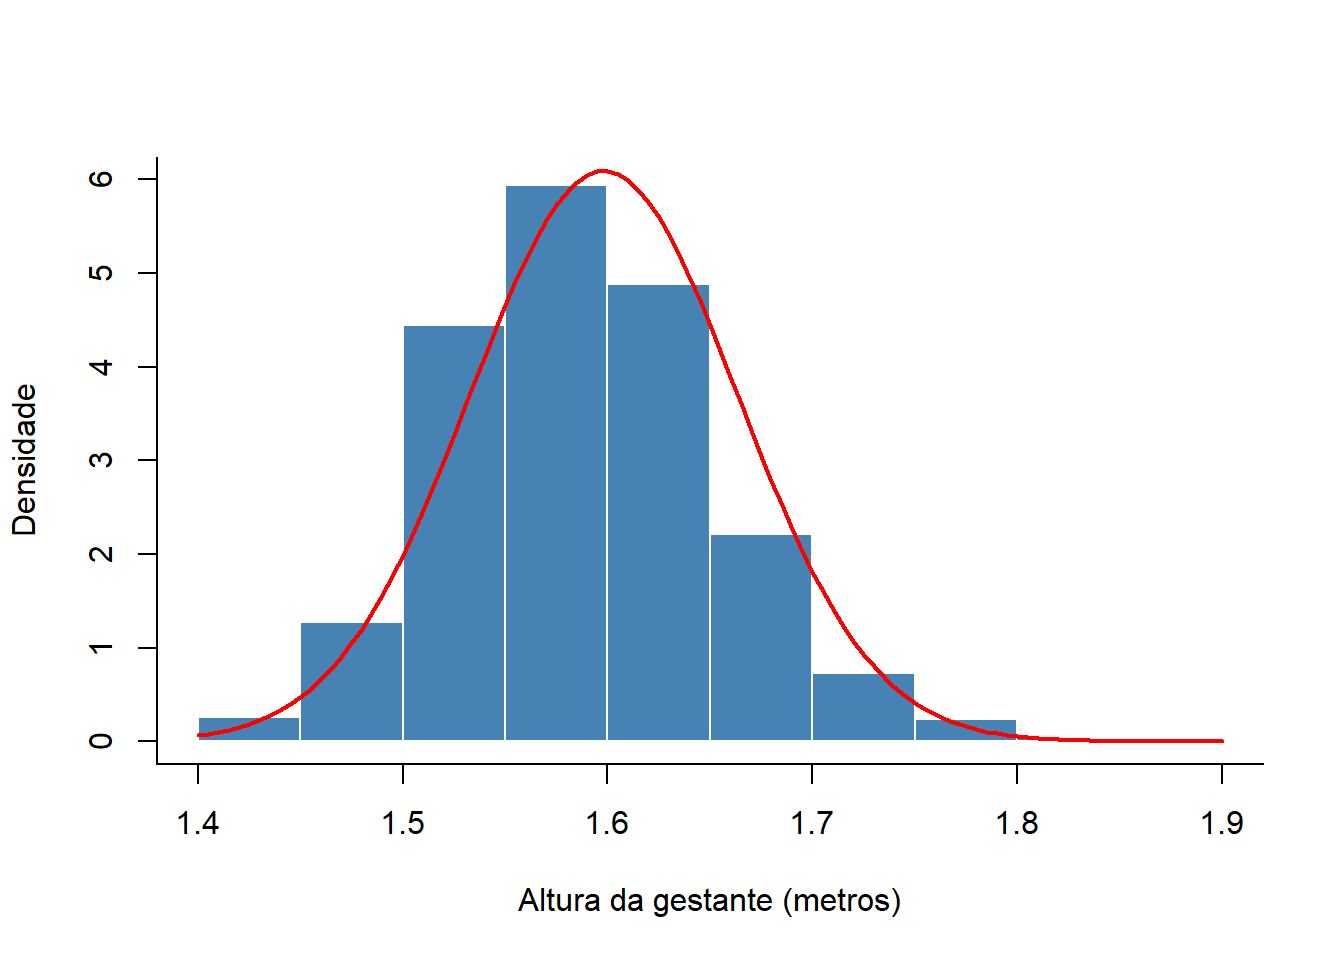
\includegraphics[width=0.8\linewidth,height=0.8\textheight]{bookdownproj_files/figure-latex/histnormal-1} 

}

\caption{Histograma com curva normal sobreposta}\label{fig:histnormal}
\end{figure}

\subsubsection{Componentes do Histograma}\label{componentes-do-histograma}

Para verificar a lista de componentes de um histograma , há necessidade de colocar o histograma da Figura \ref{fig:histh} em um objeto, no exemplo, denominado de h:

\begin{Shaded}
\begin{Highlighting}[]
\NormalTok{h }\OtherTok{\textless{}{-}} \FunctionTok{hist}\NormalTok{(mater}\SpecialCharTok{$}\NormalTok{altura,}
          \AttributeTok{breaks =} \DecValTok{8}\NormalTok{,}
          \AttributeTok{ylim =} \FunctionTok{c}\NormalTok{ (}\DecValTok{0}\NormalTok{, }\DecValTok{450}\NormalTok{),}
          \AttributeTok{xlim =} \FunctionTok{c}\NormalTok{ (}\FloatTok{1.4}\NormalTok{, }\FloatTok{1.9}\NormalTok{),}
          \AttributeTok{main=} \ConstantTok{NULL}\NormalTok{, }
          \AttributeTok{ylab =} \StringTok{"Frequência"}\NormalTok{, }
          \AttributeTok{xlab =} \StringTok{"Altura da gestante (metros)"}\NormalTok{,}
          \AttributeTok{col =}\StringTok{"tomato"}\NormalTok{,}
          \AttributeTok{freq =} \ConstantTok{TRUE}\NormalTok{,           }
          \AttributeTok{border =} \StringTok{"white"}\NormalTok{)}
      \FunctionTok{box}\NormalTok{ (}\AttributeTok{bty =} \StringTok{"L"}\NormalTok{)}
\end{Highlighting}
\end{Shaded}

\begin{figure}[H]

{\centering 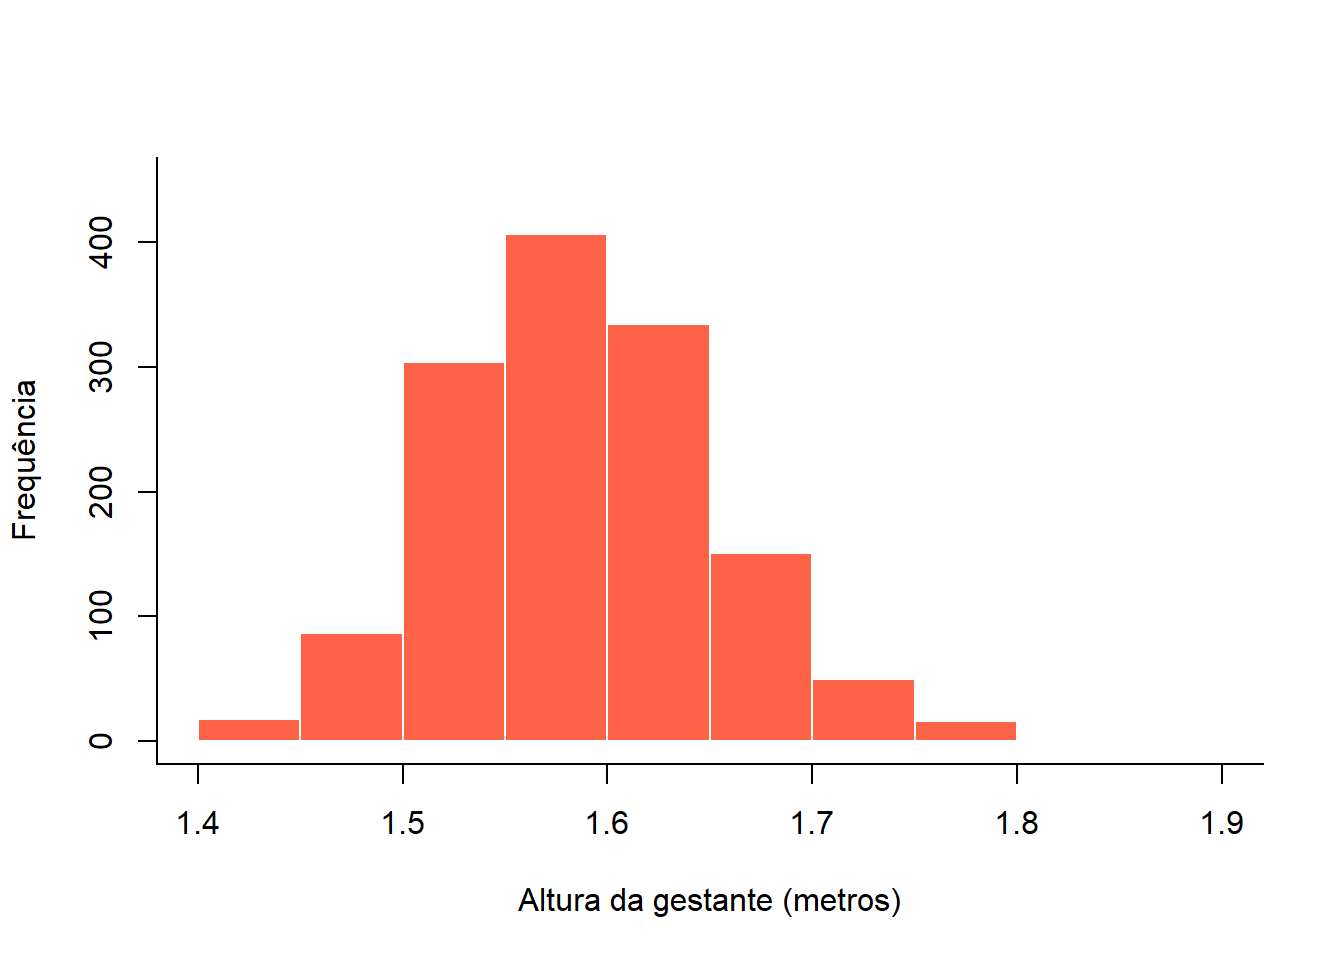
\includegraphics[width=0.8\linewidth,height=0.8\textheight]{bookdownproj_files/figure-latex/histh-1} 

}

\caption{Histograma da altura da gestante}\label{fig:histh}
\end{figure}

\begin{Shaded}
\begin{Highlighting}[]
\NormalTok{h}
\end{Highlighting}
\end{Shaded}

\begin{verbatim}
## $breaks
##  [1] 1.40 1.45 1.50 1.55 1.60 1.65 1.70 1.75 1.80 1.85
## 
## $counts
## [1]  18  87 304 406 334 151  50  16   2
## 
## $density
## [1] 0.26315789 1.27192982 4.44444444 5.93567251 4.88304094 2.20760234 0.73099415
## [8] 0.23391813 0.02923977
## 
## $mids
## [1] 1.425 1.475 1.525 1.575 1.625 1.675 1.725 1.775 1.825
## 
## $xname
## [1] "mater$altura"
## 
## $equidist
## [1] TRUE
## 
## attr(,"class")
## [1] "histogram"
\end{verbatim}

Uma das utilidades dos componentes, é construir um histograma com os valores correspondentes as barras sobrepostos ao gráfico (Figura \ref{fig:histfreq}).

\begin{Shaded}
\begin{Highlighting}[]
\FunctionTok{hist}\NormalTok{(mater}\SpecialCharTok{$}\NormalTok{altura,}
     \AttributeTok{breaks =} \DecValTok{8}\NormalTok{,}
     \AttributeTok{ylim =} \FunctionTok{c}\NormalTok{ (}\DecValTok{0}\NormalTok{, }\DecValTok{450}\NormalTok{),}
     \AttributeTok{xlim =} \FunctionTok{c}\NormalTok{ (}\FloatTok{1.4}\NormalTok{, }\FloatTok{1.9}\NormalTok{),}
     \AttributeTok{main=} \ConstantTok{NULL}\NormalTok{, }
     \AttributeTok{ylab =} \StringTok{"Frequência"}\NormalTok{, }
     \AttributeTok{xlab =} \StringTok{"Altura da gestante (metros)"}\NormalTok{,}
     \AttributeTok{col =} \StringTok{"salmon"}\NormalTok{)}
\FunctionTok{box}\NormalTok{ (}\AttributeTok{bty =} \StringTok{"L"}\NormalTok{)}

\FunctionTok{text}\NormalTok{ (h}\SpecialCharTok{$}\NormalTok{mids, h}\SpecialCharTok{$}\NormalTok{counts, }\AttributeTok{labels =}\NormalTok{ h}\SpecialCharTok{$}\NormalTok{counts, }\AttributeTok{adj=} \FunctionTok{c}\NormalTok{(}\FloatTok{0.5}\NormalTok{, }\SpecialCharTok{{-}}\FloatTok{0.5}\NormalTok{))}
\end{Highlighting}
\end{Shaded}

\begin{figure}[H]

{\centering 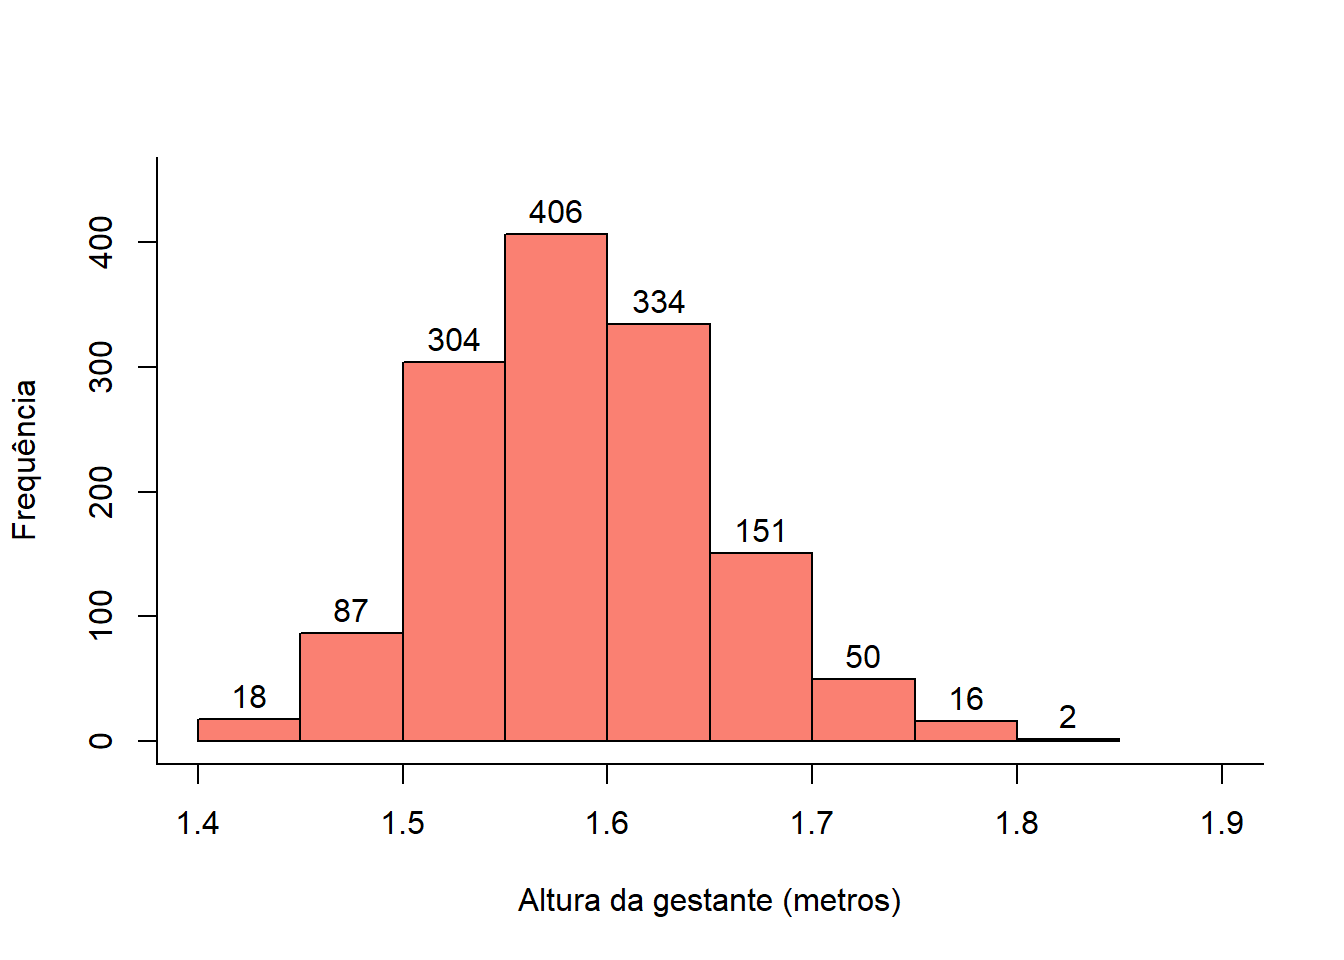
\includegraphics[width=0.8\linewidth,height=0.8\textheight]{bookdownproj_files/figure-latex/histfreq-1} 

}

\caption{Histograma com frequência sobreposta}\label{fig:histfreq}
\end{figure}

Note que as informações deste gráfico são as mesmas de uma tabela de frequência construída com os mesmos dados. Maneiras diferentes de informar uma distribuição de frequência (veja seção sobre tabelas de frequência).

\subsection{Boxplot}\label{sec-bxp}

O \emph{boxplot} descreve a distribuição de uma variável contínua exibindo o resumo de cinco números: mínimo, 1º quartil (percentil 25), mediana (percentil 50), 3ª quartil (percentil 75) e máximo (Figura \ref{fig:boxplot}).

\begin{figure}[H]

{\centering \includegraphics[width=0.7\linewidth,height=0.7\textheight]{https://i.imgur.com/Dh2UszX} 

}

\caption{Boxplot}\label{fig:boxplot}
\end{figure}

\subsubsection{Boxplot a partir de um vetor}\label{boxplot-a-partir-de-um-vetor}

Para construir um boxplot, serão usados os mesmos dados dos recém-nascidos a termo, filtrados do conjunto de dados \texttt{dadosMater.xlsx}, como realizado na seção da construção de um gráfico de barra de erro. Os dados obtidos, novamente serão atribuídos a um objeto de nome \texttt{rnt}. A variável usada para construir o boxplot será \texttt{rnt\$pesoRN}.

\begin{Shaded}
\begin{Highlighting}[]
\NormalTok{rnt }\OtherTok{\textless{}{-}} \FunctionTok{read\_excel}\NormalTok{(}\StringTok{"Arquivos/dadosMater.xlsx"}\NormalTok{) }\SpecialCharTok{\%\textgreater{}\%} 
  \FunctionTok{select}\NormalTok{(idadeMae, altura, peso, anosEst, fumo, }
\NormalTok{         para, ig, sexo, pesoRN, compRN, utiNeo) }\SpecialCharTok{\%\textgreater{}\%} 
  \FunctionTok{filter}\NormalTok{(ig }\SpecialCharTok{\textgreater{}=} \DecValTok{37} \SpecialCharTok{\&}\NormalTok{ ig }\SpecialCharTok{\textless{}} \DecValTok{42}\NormalTok{)}
\end{Highlighting}
\end{Shaded}

O R possui uma função no pacote básico denominada \texttt{boxplot()} que será usada para construir o gráfico da Figura \ref{fig:bxp}. A função solicita vários argumentos que podem alterar a sua aparência e devem ser utilizados de acordo com necessidade:

\begin{itemize}
\tightlist
\item
  \emph{formula} \(\longrightarrow\) este parâmetro é definido como um vetor ou uma fórmula (y \textasciitilde{} grupo);
\item
  \emph{data} \(\longrightarrow\)este parâmetro define o conjunto de dados;
\item
  \emph{notch} \(\longrightarrow\) parâmetro lógico. Se TRUE um entalhe será desenhado em cada lado da caixa, representando o intervalo de confiança para a mediana. Se os entalhes de dois boxplots não se sobrepuserem, indica uma ``forte evidência'' de que as duas medianas diferem;
\item
  \emph{varwidth} \(\longrightarrow\) parâmetro lógico. Se for TRUE, as caixas serão desenhadas com larguras proporcionais às raízes quadradas do número de observações nos grupos;
\item
  \emph{border} \(\longrightarrow\)um vetor opcional de cores para os contornos dos boxplots:
\item
  \emph{main} \(\longrightarrow\) este parâmetro é o título do gráfico;
\item
  \emph{xlab}, \emph{ylab} ⟶ rótulos dos eixos x e y ;
\item
  \emph{cex} \(\longrightarrow\)ver \url{https://www.statology.org/r-plot-cex/};
\item
  \emph{las} \(\longrightarrow\)altera orientação do rótulos do eixo. Valores aceitos 0 (paralelo ao eixo), 1 (horizontal), 2 (perpendicular) e 3 (vertical);
\item
  \emph{names} \(\longrightarrow\) Este parâmetro são os rótulos dos grupos que serão mostrados em cada boxplot;
\item
  \ldots{} \(\longrightarrow\) Outros parâmetros (ver ajuda do R, digitando ?boxplot no Console)
\end{itemize}

\begin{Shaded}
\begin{Highlighting}[]
\FunctionTok{boxplot}\NormalTok{ (rnt}\SpecialCharTok{$}\NormalTok{pesoRN)}
\end{Highlighting}
\end{Shaded}

\begin{figure}[H]

{\centering \includegraphics[width=0.8\linewidth,height=0.8\textheight]{bookdownproj_files/figure-latex/bxp-1} 

}

\caption{Boxplot simples}\label{fig:bxp}
\end{figure}

Esse boxplot pode ser modificado (Figura \ref{fig:bxpmod}), alterando alguns argumentos como colocação de um título no gráfico, e rótulos nos eixos e mudança na cor. Os argumento \texttt{cex.lab}, \texttt{cex.axis} e \texttt{cex.names} estabelecem o tamanho fontes. Por exemplo, para aumentar em 20\%, usamos 1.2.

\begin{Shaded}
\begin{Highlighting}[]
\FunctionTok{boxplot}\NormalTok{ (rnt}\SpecialCharTok{$}\NormalTok{pesoRN, }
         \AttributeTok{col =} \StringTok{"lightblue2"}\NormalTok{, }
         \AttributeTok{main =} \StringTok{"RN a termo"}\NormalTok{, }
         \AttributeTok{ylab =} \StringTok{"Peso do Recém{-}nascido (g)"}\NormalTok{,}
         \AttributeTok{border =} \StringTok{"black"}\NormalTok{,}
         \AttributeTok{cex.lab =} \FloatTok{1.2}\NormalTok{, }
         \AttributeTok{cex.axis =} \DecValTok{1}\NormalTok{, }
         \AttributeTok{cex.names =} \DecValTok{1}\NormalTok{,}
         \AttributeTok{las =} \DecValTok{1}\NormalTok{)}
\end{Highlighting}
\end{Shaded}

\begin{figure}[H]

{\centering \includegraphics[width=0.8\linewidth,height=0.8\textheight]{bookdownproj_files/figure-latex/bxpmod-1} 

}

\caption{Boxplot modificado}\label{fig:bxpmod}
\end{figure}

\subsubsection{Interpretação do boxplot}\label{interpretauxe7uxe3o-do-boxplot}

O boxplot nos fornece uma análise visual da posição, dispersão, simetria, caudas e valores discrepantes (\emph{outliers}) do conjunto de dados (Figura \ref{fig:boxplot}).

\begin{itemize}
\tightlist
\item
  \textbf{Posição} -- Em relação à posição dos dados, observa-se a linha central do retângulo (a mediana ou segundo quartil).
\item
  \textbf{Dispersão} -- A dispersão dos dados pode ser representada pelo intervalo interquartil (IIQ), tamanho da caixa, que é a diferença entre o terceiro quartil (3ºQ) e o primeiro quartil (1ºQ), ou ainda pela amplitude que é calculada da seguinte maneira: valor máximo -- valor mínimo. Embora a amplitude seja de fácil entendimento, o intervalo interquartil é uma estatística mais robusta para medir variabilidade uma vez que não sofre influência de \emph{outliers}.
\item
  \textbf{Simetria} -- Um conjunto de dados que tem uma distribuição simétrica, terá a linha da mediana no centro do retângulo. Quando a linha da mediana está próxima ao primeiro quartil, os dados são assimétricos positivos e quando a posição da linha da mediana é próxima ao terceiro quartil, os dados são assimétricos negativos. Vale lembrar que a mediana é a medida de tendência central mais indicada quando os dados possuem distribuição assimétrica, uma vez que a média aritmética é influenciada pelos valores extremos.
\item
  \textbf{Caudas} -- As linhas que vão do retângulo até aos outliers podem fornecer o comprimento das caudas da distribuição.
\item
  \textbf{Valores atípicos} (\emph{Outliers}) -- Os outliers indicam possíveis valores discrepantes. No boxplot, as observações são consideradas \emph{outliers} quando estão abaixo ou acima dos limites superior e inferior. O limite de detecção de outliers é construído utilizando o intervalo interquartil, dado pela distância entre o primeiro e o terceiro quartil. Sendo assim, os limites inferior e superior de detecção de outlier são dados por:
  o \emph{Limite Inferior}: 1ºQ -- (1,5 * IIQ);
  o \emph{Limite Superior}: 3ºQ + (1,5 * IIQ). Tanto o limite superior como o inferior são representados por (º).
  o Valores extremos: Valores que estão acima ou abaixo de 3 vezes o IIQ são considerados extremos, representados por (*).
\end{itemize}

\subsubsection{Adicionando pontos ao boxplot}\label{adicionando-pontos-ao-boxplot}

Quando se observa um boxplot, verifica-se que os mesmos ocultam a distribuição subjacente dos dados. Para resolver este ``problema'', pode-se adicionar pontos ao gráfico, usando a função \texttt{stripchart()}. Esta função permite criar um gráfico de dispersão unidimensional sobreposto ao boxplot (Figura \ref{fig:boxstrip}). Os comandos para esta ação são:

\begin{Shaded}
\begin{Highlighting}[]
\FunctionTok{boxplot}\NormalTok{ (rnt}\SpecialCharTok{$}\NormalTok{pesoRN, }
          \AttributeTok{col =} \StringTok{"lightblue2"}\NormalTok{, }
          \AttributeTok{ylab =} \StringTok{"Peso do Recém{-}nascido (g)"}\NormalTok{, }
          \AttributeTok{border =} \StringTok{"black"}\NormalTok{,}
          \AttributeTok{cex.lab =} \FloatTok{1.2}\NormalTok{, }
          \AttributeTok{cex.axis =} \DecValTok{1}\NormalTok{, }
          \AttributeTok{cex.names =} \DecValTok{1}\NormalTok{,}
          \AttributeTok{las =} \DecValTok{1}\NormalTok{)}

 \FunctionTok{stripchart}\NormalTok{(}\AttributeTok{x=}\NormalTok{ rnt}\SpecialCharTok{$}\NormalTok{pesoRN, }
            \AttributeTok{method =} \StringTok{"jitter"}\NormalTok{, }
            \AttributeTok{col =} \StringTok{"tomato"}\NormalTok{,}
            \AttributeTok{cex =} \FloatTok{0.5}\NormalTok{,}
            \AttributeTok{pch =} \DecValTok{16}\NormalTok{,}
            \AttributeTok{vertical =} \ConstantTok{TRUE}\NormalTok{, }
            \AttributeTok{add =} \ConstantTok{TRUE}\NormalTok{)}
\end{Highlighting}
\end{Shaded}

\begin{figure}[H]

{\centering \includegraphics[width=0.8\linewidth,height=0.8\textheight]{bookdownproj_files/figure-latex/boxstrip-1} 

}

\caption{Boxplot com pontos de dispersão}\label{fig:boxstrip}
\end{figure}

Neste exemplo, há uma grande sobreposição de pontos, pois a amostra é muito grande (n = 1085). Isto dificulta um pouco a visualização, mas ajuda a ver como a dispersão se comporta.
Você também pode personalizar o símbolo (pontos) para criar o gráfico, a largura da linha e sua cor com os argumentos \texttt{pch}, \texttt{lwd} e \texttt{col}, respectivamente. Alguns símbolos, como \texttt{pch\ =\ 21} a \texttt{25} permitem que você modifique a cor de fundo do símbolo com o argumento \texttt{bg}. O argumento \texttt{vertical\ =\ TRUE}, coloca os pontos na vertical sobreposto ao boxplot, quando o argumento \texttt{add\ =\ TRUE}. O argumento \texttt{cex\ =\ 0.5} é o tamanho dos pontos e \texttt{method\ =\ "jitter"}, espalha os pontos para diminuir a sobreposição entre eles.

\subsubsection{Boxplot com intervalos de confiança para a mediana}\label{boxplot-com-intervalos-de-confianuxe7a-para-a-mediana}

É possível representar os intervalos de confiança de 95\% para a mediana em um boxplot (Figura \ref{fig:boxnotch}), definindo o argumento \texttt{notch} como \texttt{TRUE}.

\begin{Shaded}
\begin{Highlighting}[]
\FunctionTok{boxplot}\NormalTok{ (rnt}\SpecialCharTok{$}\NormalTok{pesoRN, }
          \AttributeTok{col =} \StringTok{"lightblue2"}\NormalTok{, }
          \AttributeTok{ylab =} \StringTok{"Peso do Recém{-}nascido (g)"}\NormalTok{, }
          \AttributeTok{border =} \StringTok{"black"}\NormalTok{,}
          \AttributeTok{cex.lab =} \FloatTok{1.2}\NormalTok{, }
          \AttributeTok{cex.axis =} \DecValTok{1}\NormalTok{, }
          \AttributeTok{cex.names =} \DecValTok{1}\NormalTok{,}
          \AttributeTok{las =} \DecValTok{1}\NormalTok{,}
          \AttributeTok{notch =} \ConstantTok{TRUE}\NormalTok{)}
\end{Highlighting}
\end{Shaded}

\begin{figure}[H]

{\centering \includegraphics[width=0.8\linewidth,height=0.8\textheight]{bookdownproj_files/figure-latex/boxnotch-1} 

}

\caption{Boxplot modificado}\label{fig:boxnotch}
\end{figure}

\subsubsection{Estatísticas do boxplot}\label{estatuxedsticas-do-boxplot}

A função \texttt{boxplot.stats()} do pacote \texttt{grDevices} fornece as estatísticas do boxplot, facilitando a interpretação do mesmo, de modo semelhante ao visto para o histograma.

\begin{Shaded}
\begin{Highlighting}[]
\FunctionTok{boxplot.stats}\NormalTok{ (rnt}\SpecialCharTok{$}\NormalTok{pesoRN)}
\end{Highlighting}
\end{Shaded}

\begin{verbatim}
## $stats
## [1] 2051 2920 3215 3505 4380
## 
## $n
## [1] 1085
## 
## $conf
## [1] 3186.939 3243.061
## 
## $out
##  [1] 1440 1980 1795 1810 4400 4950 4535 4670 1425 4410 4660 1715 1895 4485 4390
## [16] 4445 4620 1785
\end{verbatim}

\textbf{Interpretação}\\
* \$stats = é o resumo dos 5 números: mínimo, percentil 25, mediana, percentil 75 e máximo;\\
* \$n = nº de obs;\\
* \$conf = limite inf/sup do entalhe se houver;\\
* \$out = são os \emph{outliers}.

\subsubsection{Múltiplos boxplots}\label{muxfaltiplos-boxplots}

Os boxplots são muito usados na comparação de grupos. A necessidade mais comum é ordenar as categorias de acordo com o aumento da mediana, mas isto é opcional. Permite identificar rapidamente qual grupo tem o maior valor e como as categorias são classificadas (Figura \ref{fig:bxpm}).\\
Será realizada uma comparação visual, usando boxplots, dos pesos dos recém-nascidos por sexo. As variáveis são \texttt{rnt\$pesoRN} e \texttt{rnt\$sexo}. Esta última está codificada como numérica 1 e 2, portanto há necessidade de ser transformada em fator:

\begin{Shaded}
\begin{Highlighting}[]
\NormalTok{rnt}\SpecialCharTok{$}\NormalTok{sexo }\OtherTok{\textless{}{-}} \FunctionTok{factor}\NormalTok{(rnt}\SpecialCharTok{$}\NormalTok{sexo,}
                   \AttributeTok{levels =} \FunctionTok{c}\NormalTok{(}\DecValTok{1}\NormalTok{, }\DecValTok{2}\NormalTok{),}
                   \AttributeTok{labels =} \FunctionTok{c}\NormalTok{(}\StringTok{"masc"}\NormalTok{, }\StringTok{"fem"}\NormalTok{))}
\end{Highlighting}
\end{Shaded}

\begin{Shaded}
\begin{Highlighting}[]
\FunctionTok{boxplot}\NormalTok{ (rnt}\SpecialCharTok{$}\NormalTok{pesoRN }\SpecialCharTok{\textasciitilde{}}\NormalTok{ rnt}\SpecialCharTok{$}\NormalTok{sexo, }
         \AttributeTok{col =} \FunctionTok{c}\NormalTok{(}\StringTok{"lightblue2"}\NormalTok{, }\StringTok{"pink"}\NormalTok{), }
         \AttributeTok{ylab =} \StringTok{"Peso do Recém{-}nascido (g)"}\NormalTok{, }
         \AttributeTok{xlab =} \StringTok{"Sexo"}\NormalTok{,}
         \AttributeTok{ylim =} \FunctionTok{c}\NormalTok{(}\DecValTok{1000}\NormalTok{, }\DecValTok{5000}\NormalTok{),}
         \AttributeTok{border =} \StringTok{"black"}\NormalTok{,}
         \AttributeTok{cex.lab =} \DecValTok{1}\NormalTok{, }
         \AttributeTok{cex.axis =} \DecValTok{1}\NormalTok{, }
         \AttributeTok{cex.names =} \DecValTok{1}\NormalTok{,}
         \AttributeTok{las =} \DecValTok{1}\NormalTok{)}
\end{Highlighting}
\end{Shaded}

\begin{figure}[H]

{\centering \includegraphics[width=0.8\linewidth,height=0.8\textheight]{bookdownproj_files/figure-latex/bxpm-1} 

}

\caption{Múltiplos boxplots}\label{fig:bxpm}
\end{figure}

Observe que foi utilizado o argumento \texttt{rnt\$pesoRN\ \textasciitilde{}\ rnt\$sexo} (\emph{y \textasciitilde{} grupo}) para obter os dois boxplots. Existe uma pequena diferença entre eles, as caixas são quase coincidentes.. Foi suprimido o argumento (\texttt{xlab\ =\ sexo}) relativo ao rótulo do eixo \emph{x}, pois seria redundante.

Pode-se fazer um entalhe (\emph{notch}) que podem ser interpretados como um intervalo de confiança em torno dos valores medianos (Figura \ref{fig:bxpnotch}). É calculado pela fórmula :\(mediana \pm 1.57\times IIQ/\sqrt{n}\). No nosso exemplo, observe que o entalhe nos meninos está um pouco acima do das meninas..

\begin{Shaded}
\begin{Highlighting}[]
\FunctionTok{boxplot}\NormalTok{ (rnt}\SpecialCharTok{$}\NormalTok{pesoRN }\SpecialCharTok{\textasciitilde{}}\NormalTok{ rnt}\SpecialCharTok{$}\NormalTok{sexo, }
         \AttributeTok{col =} \FunctionTok{c}\NormalTok{(}\StringTok{"lightblue2"}\NormalTok{, }\StringTok{"pink"}\NormalTok{), }
         \AttributeTok{ylab =} \StringTok{"Peso do Recém{-}nascido (g)"}\NormalTok{, }
         \AttributeTok{xlab =} \StringTok{"Sexo"}\NormalTok{,}
         \AttributeTok{ylim =} \FunctionTok{c}\NormalTok{(}\DecValTok{1000}\NormalTok{, }\DecValTok{5000}\NormalTok{),}
         \AttributeTok{border =} \StringTok{"black"}\NormalTok{,}
         \AttributeTok{cex.lab =} \DecValTok{1}\NormalTok{, }
         \AttributeTok{cex.axis =} \DecValTok{1}\NormalTok{, }
         \AttributeTok{cex.names =} \DecValTok{1}\NormalTok{,}
         \AttributeTok{las =} \DecValTok{1}\NormalTok{,}
         \AttributeTok{notch =} \ConstantTok{TRUE}\NormalTok{)}
\end{Highlighting}
\end{Shaded}

\begin{figure}[H]

{\centering \includegraphics[width=0.8\linewidth,height=0.8\textheight]{bookdownproj_files/figure-latex/bxpnotch-1} 

}

\caption{Boxplots com entalhes}\label{fig:bxpnotch}
\end{figure}

\subsubsection{Boxplots horizontais}\label{boxplots-horizontais}

Para criar um boxplot horizontal (Figura \ref{fig:bxph}), usamos o argumento \texttt{horizontal\ =\ TRUE} e invertemos os rotulos dos eixos \emph{x} e \emph{y}.

\begin{Shaded}
\begin{Highlighting}[]
\FunctionTok{boxplot}\NormalTok{ (rnt}\SpecialCharTok{$}\NormalTok{pesoRN }\SpecialCharTok{\textasciitilde{}}\NormalTok{ rnt}\SpecialCharTok{$}\NormalTok{sexo, }
         \AttributeTok{col =} \FunctionTok{c}\NormalTok{(}\StringTok{"lightblue2"}\NormalTok{, }\StringTok{"pink2"}\NormalTok{), }
         \AttributeTok{xlab =} \StringTok{"Peso do Recém{-}nascido (g)"}\NormalTok{, }
         \AttributeTok{ylab =} \ConstantTok{NULL}\NormalTok{,}
         \AttributeTok{horizontal =} \ConstantTok{TRUE}\NormalTok{,}
         \AttributeTok{border =} \StringTok{"black"}\NormalTok{,}
         \AttributeTok{cex.lab =} \FloatTok{1.2}\NormalTok{, }
         \AttributeTok{cex.axis =} \DecValTok{1}\NormalTok{, }
         \AttributeTok{cex.names =} \DecValTok{1}\NormalTok{,}
         \AttributeTok{las =} \DecValTok{1}\NormalTok{)}
\end{Highlighting}
\end{Shaded}

\begin{figure}[H]

{\centering \includegraphics[width=0.8\linewidth,height=0.8\textheight]{bookdownproj_files/figure-latex/bxph-1} 

}

\caption{Boxplots horizontais}\label{fig:bxph}
\end{figure}

\subsection{Gráfico de Dispersão}\label{gruxe1fico-de-dispersuxe3o}

Um gráfico de dispersão (\emph{Scatterplot}) exibe a relação entre duas variáveis numéricas (Figura \ref{fig:scatter}). Cada ponto representa uma observação. Suas posições nos eixos \emph{x} (horizontal) e \emph{y} (vertical) representam os valores das duas variáveis.

O R Base é uma boa opção para construir um gráfico de dispersão, usando a função \texttt{plot()}. Ambas as variáveis numéricas do banco de dados devem ser especificadas nos argumentos \emph{x} e \emph{y}.

A função \texttt{plot()} é uma função genérica que pode ser facilmente editada com múltiplos argumentos envolvendo os eixos e caracteres plotados da mesma maneira que foi feita com os gráficos anteriores. Aqui, novamente, serão usados os dados incluídos no conjunto de dados \texttt{rnt}:

\begin{Shaded}
\begin{Highlighting}[]
\FunctionTok{plot}\NormalTok{ (}\AttributeTok{x =}\NormalTok{ rnt}\SpecialCharTok{$}\NormalTok{compRN,}
      \AttributeTok{y =}\NormalTok{ rnt}\SpecialCharTok{$}\NormalTok{pesoRN,}
      \AttributeTok{ylab =} \StringTok{"Peso de Recém{-}nascido (g)"}\NormalTok{,}
      \AttributeTok{xlab =} \StringTok{"Comprimento do Recém{-}nascido (cm)"}\NormalTok{,}
      \AttributeTok{cex.axis =} \FloatTok{0.8}\NormalTok{,}
      \AttributeTok{las =} \DecValTok{1}\NormalTok{)}
\end{Highlighting}
\end{Shaded}

\begin{figure}[H]

{\centering \includegraphics[width=0.8\linewidth,height=0.8\textheight]{bookdownproj_files/figure-latex/scatter-1} 

}

\caption{Gráfico de dispersão}\label{fig:scatter}
\end{figure}

Este mesmo gráfico pode ser obtido, usando uma fórmula \texttt{y\textasciitilde{}x} e acrescentando o argumento \texttt{bty\ =\ "L"} (Figura \ref{fig:scatter1}). Este argumento permite personalizar a caixa ao redor do gráfico.

\begin{itemize}
\tightlist
\item
  \emph{o}: caixa completa (parâmetro padrão),
\item
  \emph{n}: sem caixa
\item
  \emph{7}: superior + direita
\item
  \emph{L}: inferior + esquerda
\item
  \emph{C}: superior + esquerda + inferior
\item
  \emph{U}: esquerda + inferior + direita
\end{itemize}

\begin{Shaded}
\begin{Highlighting}[]
\FunctionTok{plot}\NormalTok{ (pesoRN }\SpecialCharTok{\textasciitilde{}}\NormalTok{ compRN,}
      \AttributeTok{data =}\NormalTok{ rnt,}
      \AttributeTok{ylab =} \StringTok{"Peso de Recém{-}nascido (g)"}\NormalTok{,}
      \AttributeTok{xlab =} \StringTok{"Comprimento do Recém{-}nascido (cm)"}\NormalTok{,}
      \AttributeTok{cex.axis =} \FloatTok{0.8}\NormalTok{,}
      \AttributeTok{las =} \DecValTok{1}\NormalTok{,}
      \AttributeTok{bty =} \StringTok{"L"}\NormalTok{)}
\end{Highlighting}
\end{Shaded}

\begin{figure}[H]

{\centering \includegraphics[width=0.8\linewidth,height=0.8\textheight]{bookdownproj_files/figure-latex/scatter1-1} 

}

\caption{Gráfico de dispersão}\label{fig:scatter1}
\end{figure}

Como em qualquer outro gráfico, este também pode ser melhorado em seu aspecto, tornando os pontos sólidos e coloridos. O argumento \texttt{pch} estabelece o tipo de pontos (Figura \ref{fig:pch}).

\begin{figure}[H]

{\centering \includegraphics[width=0.65\linewidth]{https://i.imgur.com/8VWZSGk} 

}

\caption{Símbolo dos formatos}\label{fig:pch}
\end{figure}

Na Figura \ref{fig:scatter}, como os pontos estão aglomerados, devido a quantidade, é possível tentar espalhá-los, usando a função \texttt{jitter()} na variável \texttt{compRN} (Figura \ref{fig:jitter}). O argumento 10 é variável e significa o grau de espalhamento:

\begin{Shaded}
\begin{Highlighting}[]
\FunctionTok{plot}\NormalTok{ (}\FunctionTok{jitter}\NormalTok{(rnt}\SpecialCharTok{$}\NormalTok{compRN,}\DecValTok{10}\NormalTok{),}
\NormalTok{      rnt}\SpecialCharTok{$}\NormalTok{pesoRN,}
      \AttributeTok{col =} \StringTok{"steelblue"}\NormalTok{,}
      \AttributeTok{ylab =} \StringTok{"Peso de Recém{-}nascido (g)"}\NormalTok{,}
      \AttributeTok{xlab =} \StringTok{"Comprimento do Recém{-}nascido (cm)"}\NormalTok{,}
      \AttributeTok{las =} \DecValTok{1}\NormalTok{,}
      \AttributeTok{bty =} \StringTok{"L"}\NormalTok{,}
      \AttributeTok{pch =} \DecValTok{16}\NormalTok{,}
      \AttributeTok{cex =} \DecValTok{1}\NormalTok{,}
      \AttributeTok{cex.lab =} \FloatTok{1.1}\NormalTok{,}
      \AttributeTok{cex.axis =} \FloatTok{0.8}\NormalTok{)}
\end{Highlighting}
\end{Shaded}

\begin{figure}[H]

{\centering \includegraphics[width=0.8\linewidth,height=0.8\textheight]{bookdownproj_files/figure-latex/jitter-1} 

}

\caption{Gráfico de dispersão com *jitter*}\label{fig:jitter}
\end{figure}

\subsubsection{Mapeamento dos pontos de acordo com uma variável categórica}\label{mapeamento-dos-pontos-de-acordo-com-uma-variuxe1vel-categuxf3rica}

Inicialmente, será criado um vetor para representar as cores, de acordo com o sexo (meninos = azul; meninas = vermelho). Usa-se a função \texttt{unclass()} para discriminar os sexos (Figura \ref{fig:map}). Acrescenta-se uma legenda para ilustrar a separação.

\begin{Shaded}
\begin{Highlighting}[]
\NormalTok{cores }\OtherTok{\textless{}{-}} \FunctionTok{c}\NormalTok{(}\StringTok{"dodgerblue3"}\NormalTok{, }\StringTok{"tomato"}\NormalTok{)}

\FunctionTok{plot}\NormalTok{(}\AttributeTok{x =} \FunctionTok{jitter}\NormalTok{(rnt}\SpecialCharTok{$}\NormalTok{compRN, }\DecValTok{10}\NormalTok{), }
  \AttributeTok{y =}\NormalTok{ rnt}\SpecialCharTok{$}\NormalTok{pesoRN,}
  \AttributeTok{bg =}\NormalTok{ cores[}\FunctionTok{unclass}\NormalTok{(rnt}\SpecialCharTok{$}\NormalTok{sexo)],}
  \AttributeTok{ylab =} \StringTok{"Peso de Recém{-}nascido (g)"}\NormalTok{,}
  \AttributeTok{xlab =} \StringTok{"Comprimento do Recém{-}nascido (cm)"}\NormalTok{,}
  \AttributeTok{las =} \DecValTok{1}\NormalTok{,}
  \AttributeTok{bty =} \StringTok{"L"}\NormalTok{,}
  \AttributeTok{cex =} \FloatTok{1.5}\NormalTok{,}
  \AttributeTok{pch=}\DecValTok{21}\NormalTok{,}
  \AttributeTok{cex.lab =} \DecValTok{1}\NormalTok{,}
  \AttributeTok{cex.axis =} \FloatTok{0.8}\NormalTok{)}

\FunctionTok{legend}\NormalTok{ (}\AttributeTok{legend =} \FunctionTok{c}\NormalTok{(}\StringTok{"Meninos"}\NormalTok{, }\StringTok{"Meninas"}\NormalTok{), }
        \AttributeTok{fill =}\NormalTok{ cores, }
        \AttributeTok{bty=}\StringTok{"n"}\NormalTok{, }
        \AttributeTok{cex =} \DecValTok{1}\NormalTok{,}
        \StringTok{"topleft"}\NormalTok{)}
\end{Highlighting}
\end{Shaded}

\begin{figure}[H]

{\centering \includegraphics[width=0.8\linewidth,height=0.8\textheight]{bookdownproj_files/figure-latex/map-1} 

}

\caption{Mapeamento dos pontos de acordo com uma variável categórica}\label{fig:map}
\end{figure}

\subsubsection{Adição da reta de ajuste}\label{adiuxe7uxe3o-da-reta-de-ajuste}

Uma linha reta de ajuste dos dados (Figura \ref{fig:reta}) pode ser acrescentada usando a função \texttt{abline\ ()}, associada a função \texttt{lm\ ()}. Um modelo típico lm (\emph{linear model}) tem o formato \emph{resposta (}y\emph{) \textasciitilde{} preditor (}x\emph{)}. Mais detalhes sobre o modelo de ajuste linear na regressão linear (veja capítulo 15).

\begin{Shaded}
\begin{Highlighting}[]
\CommentTok{\# Construção do gráfico de dispersão}
\FunctionTok{plot}\NormalTok{ (}\FunctionTok{jitter}\NormalTok{(rnt}\SpecialCharTok{$}\NormalTok{compRN,}\DecValTok{10}\NormalTok{),}
\NormalTok{      rnt}\SpecialCharTok{$}\NormalTok{pesoRN,}
      \AttributeTok{col =} \StringTok{"gray40"}\NormalTok{,}
      \AttributeTok{bg =} \StringTok{"darkturquoise"}\NormalTok{,}
      \AttributeTok{ylab =} \StringTok{"Peso de Recém{-}nascido (g)"}\NormalTok{,}
      \AttributeTok{xlab =} \StringTok{"Comprimento do Recém{-}nascido (cm)"}\NormalTok{,}
      \AttributeTok{las =} \DecValTok{1}\NormalTok{,}
      \AttributeTok{bty =} \StringTok{"L"}\NormalTok{,}
      \AttributeTok{pch =} \DecValTok{21}\NormalTok{,}
      \AttributeTok{cex =} \FloatTok{1.3}\NormalTok{,}
      \AttributeTok{cex.lab =} \DecValTok{1}\NormalTok{,}
      \AttributeTok{cex.axis =} \FloatTok{0.8}\NormalTok{)}

\CommentTok{\# Criação do modelo de ajuste}
\NormalTok{modelo }\OtherTok{\textless{}{-}} \FunctionTok{lm}\NormalTok{ (rnt}\SpecialCharTok{$}\NormalTok{pesoRN }\SpecialCharTok{\textasciitilde{}}\NormalTok{ rnt}\SpecialCharTok{$}\NormalTok{compRN)}

\CommentTok{\# Adição da reta, usando o modelo}
\FunctionTok{abline}\NormalTok{ (modelo, }
        \AttributeTok{col=}\StringTok{"red"}\NormalTok{, }
        \AttributeTok{lwd=}\DecValTok{2}\NormalTok{, }
        \AttributeTok{lty =} \DecValTok{2}\NormalTok{)}
\end{Highlighting}
\end{Shaded}

\begin{figure}[H]

{\centering \includegraphics[width=0.8\linewidth,height=0.8\textheight]{bookdownproj_files/figure-latex/reta-1} 

}

\caption{Gráfico de dispersão com reta de ajuste}\label{fig:reta}
\end{figure}

Ao executar o modelo, se obtém os parâmetros para a construção da equação da regressão linear:

\begin{Shaded}
\begin{Highlighting}[]
\FunctionTok{summary}\NormalTok{(modelo)}
\end{Highlighting}
\end{Shaded}

\begin{verbatim}
## 
## Call:
## lm(formula = rnt$pesoRN ~ rnt$compRN)
## 
## Residuals:
##      Min       1Q   Median       3Q      Max 
## -1434.56  -218.40   -19.56   177.76  2097.87 
## 
## Coefficients:
##              Estimate Std. Error t value Pr(>|t|)    
## (Intercept) -3416.451    215.821  -15.83   <2e-16 ***
## rnt$compRN    137.674      4.475   30.77   <2e-16 ***
## ---
## Signif. codes:  0 '***' 0.001 '**' 0.01 '*' 0.05 '.' 0.1 ' ' 1
## 
## Residual standard error: 337.7 on 1083 degrees of freedom
## Multiple R-squared:  0.4664, Adjusted R-squared:  0.4659 
## F-statistic: 946.6 on 1 and 1083 DF,  p-value: < 2.2e-16
\end{verbatim}

A equação de predição da regressão linear permite que ao conhecer o valor do comprimento é possível prever o peso do recem-nascido:

\[
\hat{y} = b_{0}+ b_{1}\times x
\]

Desta forma, substituindo pelos valores contidos nas estimativas da tabela dos coeficientes do sumário do modelo, um bebê com 50 cm terá um peso de aproximadamente:

\[
\hat{y} = -3416.45 + 137.67\times 50 = 3467.05
\]

\section{\texorpdfstring{Introdução ao \texttt{ggplot2}}{Introdução ao ggplot2}}\label{sec-ggplot2}

O R tem vários sistemas para fazer gráficos e, na ,maioria das vezes, eles são suficientes. Entretanto, o surgimento do \texttt{ggplot2} \citet{wickham2016ggplot2} trouxe a possibilidade de serem construídos gráficos mais elegantes e versáteis. Além disso, torna o processo mais rápido, baseado uma sofisticada gramática \citep{wickham2010layered}.

O gráfico é construído, usando função \texttt{ggplot()}, a partir de alguns elementos básicos \footnote{O número de elementos pode variar dependendo de como você os agrupa e da pergunta a ser respondida.}:

\begin{itemize}
\tightlist
\item
  \emph{Dados} \(\longrightarrow\) os dados brutos que você deseja representar graficamente.
\item
  \emph{Geometria} (\emph{geoms}) \(\longrightarrow\) As formas geométricas que irão representar os dados.
\item
  \emph{Estética} (\emph{aes}) \(\longrightarrow\) Estética dos objetos geométricos e estatísticos, como posição, cor, tamanho, forma e transparência
\item
  \emph{Escala} (\emph{scales}) \(\longrightarrow\) Mapas entre os dados e as dimensões estéticas, como intervalo de dados para plotar largura ou valores de fator para cores.
\item
  \emph{Transformações estatísticas} (\emph{stats}) \(\longrightarrow\) resumos estatísticos dos dados, como quantis, curvas ajustadas e somas.
\item
  \emph{Sistemas de coordenadas} (\emph{coordinates Systems}) \(\longrightarrow\) A transformação usada para mapear coordenadas de dados no plano do retângulo de dados.
\item
  \emph{Facetas} (\emph{faceting}) \(\longrightarrow\) A organização dos dados em uma grade de gráficos.
\item
  \emph{Temas visuais} (\emph{themes}) \(\longrightarrow\) Os padrões visuais gerais de um gráfico, como plano de fundo, grades, eixos, tipo de letra padrão, tamanhos e cores.
\end{itemize}

\subsection{Dados usados nesta seção}\label{dados-usados-nesta-seuxe7uxe3o-2}

Serão usados os mesmos dados do conjunto \texttt{rnt}, acrescidos da variável \texttt{categIdade} (idade categorizada) e da variável categEscola (anos de estudo completos categorizados).

\begin{Shaded}
\begin{Highlighting}[]
\NormalTok{ rnt}\SpecialCharTok{$}\NormalTok{categIdade }\OtherTok{\textless{}{-}} \FunctionTok{cut}\NormalTok{(rnt}\SpecialCharTok{$}\NormalTok{idadeMae,}
                       \AttributeTok{breaks =} \FunctionTok{c}\NormalTok{(}\DecValTok{13}\NormalTok{, }\DecValTok{20}\NormalTok{, }\DecValTok{36}\NormalTok{, }\DecValTok{46}\NormalTok{),}
                       \AttributeTok{labels =} \FunctionTok{c}\NormalTok{(}\StringTok{"\textless{}20a"}\NormalTok{, }\StringTok{"20{-}35a"}\NormalTok{, }\StringTok{"\textgreater{}35a"}\NormalTok{),}
                       \AttributeTok{include.lowest =} \ConstantTok{TRUE}\NormalTok{,}
                       \AttributeTok{right =} \ConstantTok{FALSE}\NormalTok{,}
                       \AttributeTok{ordered\_result =}\ConstantTok{TRUE}\NormalTok{)}


\NormalTok{ rnt}\SpecialCharTok{$}\NormalTok{categEscola }\OtherTok{\textless{}{-}} \FunctionTok{cut}\NormalTok{ (rnt}\SpecialCharTok{$}\NormalTok{anosEst,}
                         \AttributeTok{breaks=} \FunctionTok{c}\NormalTok{ (}\DecValTok{0}\NormalTok{,}\DecValTok{10}\NormalTok{,}\DecValTok{13}\NormalTok{,}\DecValTok{18}\NormalTok{),}
                         \AttributeTok{right =} \ConstantTok{FALSE}\NormalTok{,}
                         \AttributeTok{labels =} \FunctionTok{c}\NormalTok{(}\StringTok{"Fundamental"}\NormalTok{,}
                                     \StringTok{"Médio"}\NormalTok{,}
                                     \StringTok{"Superior"}\NormalTok{),}
                         \AttributeTok{include.lowest =} \ConstantTok{TRUE}\NormalTok{,}
                         \AttributeTok{ordered\_result =}\ConstantTok{TRUE}\NormalTok{) }
\end{Highlighting}
\end{Shaded}

A variável \texttt{rnt\$fumo} será transformada em fator::

\begin{Shaded}
\begin{Highlighting}[]
\NormalTok{rnt}\SpecialCharTok{$}\NormalTok{fumo }\OtherTok{\textless{}{-}} \FunctionTok{factor}\NormalTok{ (rnt}\SpecialCharTok{$}\NormalTok{fumo,}
                    \AttributeTok{levels =} \FunctionTok{c}\NormalTok{(}\DecValTok{1}\NormalTok{, }\DecValTok{2}\NormalTok{),}
                    \AttributeTok{labels =} \FunctionTok{c}\NormalTok{(}\StringTok{"sim"}\NormalTok{, }\StringTok{"não"}\NormalTok{))}
\end{Highlighting}
\end{Shaded}

\subsection{Função ggplot()}\label{funuxe7uxe3o-ggplot}

A sintaxe do \texttt{ggplot2} é diferente do R básico. De acordo com os elementos básicos, um \texttt{ggplot} padrão precisa de três informações que devem ser especificadas: os \emph{dados}, a \emph{estética} e a \emph{geometria}. Essas são as camadas principais.\\
Será criado um \texttt{ggplot} padrão (Figura \ref{fig:padrao}) que será atribuído a um objeto \texttt{g}, usando \texttt{data\ =\ dados} e a estética (\texttt{aes}), no eixo \emph{x}, a variável \texttt{compRN} e, no eixo \emph{y}, a variável \texttt{pesoRN}.

\begin{Shaded}
\begin{Highlighting}[]
\NormalTok{g }\OtherTok{\textless{}{-}} \FunctionTok{ggplot}\NormalTok{ (}\AttributeTok{data =}\NormalTok{ rnt, }\FunctionTok{aes}\NormalTok{ (}\AttributeTok{x =}\NormalTok{ compRN, }\AttributeTok{y =}\NormalTok{ pesoRN))}
\NormalTok{g}
\end{Highlighting}
\end{Shaded}

\begin{figure}[H]

{\centering \includegraphics[width=0.8\linewidth,height=0.8\textheight]{bookdownproj_files/figure-latex/padrao-1} 

}

\caption{Gráfico ggplot padrão}\label{fig:padrao}
\end{figure}

A este gráfico básico ``vazio'' adiciona-se uma camada que especifique o tipo de gemometria desejada (Figura \ref{fig:layer1}). A geometria \texttt{geom\_point()} retorna um gráfico de dispersão.

\begin{Shaded}
\begin{Highlighting}[]
\NormalTok{g }\SpecialCharTok{+} \FunctionTok{geom\_point}\NormalTok{()}
\end{Highlighting}
\end{Shaded}

\begin{figure}[H]

{\centering \includegraphics[width=0.8\linewidth,height=0.8\textheight]{bookdownproj_files/figure-latex/layer1-1} 

}

\caption{Gráfico de dipersão}\label{fig:layer1}
\end{figure}

A estética (\texttt{aes}) pode ser definida tanto na camada \texttt{ggplot} como na \texttt{geom}. Especificando no \texttt{ggplot}, esta \texttt{aes} será usada em todos os outros geoms que aoarecerem. Usando no \texttt{geom}, servirá apenas para ele. No exemplo. é indiferente o local da \texttt{aes}, o resultado será o mesmo, pois existe apenas um \texttt{geom}.

\subsection{Tipos de geoms}\label{tipos-de-geoms}

Encontra-se uma grande possibilidade de geometrias, de acordo com o tipo de gráfico que será plotado. Elas podem ser visualizadas \href{https://ggplot2.tidyverse.org/reference/}{\textbf{aqui}}.

\subsubsection{Histograma}\label{histograma-1}

O \texttt{geom\_histogram()} é a geometria para a construção de um histograma. Aqui, há necessidade apenas do eixo \emph{x}, pois existe uma única variável (\texttt{pesoRN}). A execução do comando retorna a distribuição dessa variável (Figura \ref{fig:gghist}):

\begin{Shaded}
\begin{Highlighting}[]
\FunctionTok{ggplot}\NormalTok{(}\AttributeTok{data =}\NormalTok{ rnt) }\SpecialCharTok{+}
  \FunctionTok{geom\_histogram}\NormalTok{(}\FunctionTok{aes}\NormalTok{(}\AttributeTok{x =}\NormalTok{ pesoRN))}
\end{Highlighting}
\end{Shaded}

\begin{figure}[H]

{\centering \includegraphics[width=0.8\linewidth,height=0.8\textheight]{bookdownproj_files/figure-latex/gghist-1} 

}

\caption{Histograma no 'ggplot2'}\label{fig:gghist}
\end{figure}

\subsubsection{Gráfico de barras}\label{gruxe1fico-de-barras-1}

A função \texttt{geom\_bar()}permite delinear um gráfico de barras (Figura \ref{fig:ggbar}) com a variável \texttt{categIdade}:

\begin{Shaded}
\begin{Highlighting}[]
\FunctionTok{ggplot}\NormalTok{(}\AttributeTok{data =}\NormalTok{ rnt) }\SpecialCharTok{+}
  \FunctionTok{geom\_bar}\NormalTok{(}\FunctionTok{aes}\NormalTok{(}\AttributeTok{x =}\NormalTok{ categIdade, }\AttributeTok{y =} \FunctionTok{after\_stat}\NormalTok{(count}\SpecialCharTok{/}\FunctionTok{sum}\NormalTok{(count))))}
\end{Highlighting}
\end{Shaded}

\begin{figure}[H]

{\centering \includegraphics[width=0.8\linewidth,height=0.8\textheight]{bookdownproj_files/figure-latex/ggbar-1} 

}

\caption{Gráfico de barras no 'ggplot2'}\label{fig:ggbar}
\end{figure}

A função \texttt{after\_stat()} colocada no argumento \emph{y} é usada para determinar o tipo de estatística que irá aparecer no eixo \emph{y}, quando ela não está disponível nos dados. No exemplo, foi usada a proporção que cada categoria representa na variável \texttt{categIdade} (\texttt{count/sum(count}). Dessa forma, as parturientes acima de 35 anos correspondem a uma proporção de aproximadamente 0,10 (ou 10\%).

\subsubsection{Boxplot}\label{boxplot}

Com o \texttt{geom\_boxplot()}, serão criados boxplots (Figura \ref{fig:ggbxp}) comparando os pesos dos neonatos por sexo..

\begin{Shaded}
\begin{Highlighting}[]
\FunctionTok{ggplot}\NormalTok{(}\AttributeTok{data =}\NormalTok{ rnt) }\SpecialCharTok{+}
  \FunctionTok{geom\_boxplot}\NormalTok{(}\FunctionTok{aes}\NormalTok{(}\AttributeTok{x =}\NormalTok{ sexo, }\AttributeTok{y =}\NormalTok{ pesoRN))}
\end{Highlighting}
\end{Shaded}

\begin{figure}[H]

{\centering \includegraphics[width=0.8\linewidth,height=0.8\textheight]{bookdownproj_files/figure-latex/ggbxp-1} 

}

\caption{Boxplot no 'ggplot2'}\label{fig:ggbxp}
\end{figure}

\subsubsection{Gráfico de linhas}\label{gruxe1fico-de-linhas}

Os dados, para produzir o gráfico de linha com a função \texttt{geom\_line()}, podem ser obtidos \href{https://github.com/petronioliveira/Arquivos/blob/main/dadosObitos.xlsx}{\textbf{aqui}}, acessar e baixar para o seu diretório de trabalho o arquivo \texttt{dadosObitos.xlsx}. Este conjunto de dados é constituído pelos óbitos por COVID-19 no Rio Grande do Sul entre 2020 e 2022.

Atribua os dados ao objeto \texttt{obitos}, a partir do diretório de trabalho.

\begin{Shaded}
\begin{Highlighting}[]
\NormalTok{obitos }\OtherTok{\textless{}{-}} \FunctionTok{read\_excel}\NormalTok{(}\StringTok{"Arquivos/dadosObitos.xlsx"}\NormalTok{)}
\FunctionTok{str}\NormalTok{(obitos)}
\end{Highlighting}
\end{Shaded}

\begin{verbatim}
## tibble [25 x 2] (S3: tbl_df/tbl/data.frame)
##  $ data  : POSIXct[1:25], format: "2020-03-01" "2020-04-01" ...
##  $ obitos: num [1:25] 4 60 182 440 1391 ...
\end{verbatim}

Para a construção do gráfico de linha (Figura \ref{fig:ggline}), use o seguinte comando:

\begin{Shaded}
\begin{Highlighting}[]
\FunctionTok{ggplot}\NormalTok{(}\AttributeTok{data =}\NormalTok{ obitos) }\SpecialCharTok{+}
  \FunctionTok{geom\_line}\NormalTok{(}\FunctionTok{aes}\NormalTok{(}\AttributeTok{x =}\NormalTok{ data, }\AttributeTok{y =}\NormalTok{ obitos))}
\end{Highlighting}
\end{Shaded}

\begin{figure}[H]

{\centering \includegraphics[width=0.8\linewidth,height=0.8\textheight]{bookdownproj_files/figure-latex/ggline-1} 

}

\caption{Gráfico de linha no 'ggplot2'}\label{fig:ggline}
\end{figure}

\subsection{Modificação dos argumentos do geoms}\label{modificauxe7uxe3o-dos-argumentos-do-geoms}

É possível mofificar alguns argumentos no \texttt{geom}. Cada tipo de \texttt{geom} possibilita alterações específicas.

Inicialmente, serão realizadas modificações no gráfico de dispersão, construído acima com a \texttt{geom\_point}, modificando a cor, de acordo com o sexo do recém-nascido (Figura \ref{fig:point}) com o argumento \texttt{color=}:

Quando o argumento cor for colocado dentro da \texttt{aes}, ele será definido por uma variável, no caso \texttt{sexo}. Desta forma, cada um dos sexos serão representados por pontos coloridos diferentes. A escolha da cor foi automática pelo \texttt{ggplot2}, entregando duas cores conforme o padrão da sua paleta. Quando o argumento é colocado fora da estética da geom, há necessidade de escolher a cor para os pontos.

\begin{Shaded}
\begin{Highlighting}[]
\FunctionTok{ggplot}\NormalTok{(}\AttributeTok{data =}\NormalTok{ rnt) }\SpecialCharTok{+}
  \FunctionTok{geom\_point}\NormalTok{(}\FunctionTok{aes}\NormalTok{(}\AttributeTok{x =}\NormalTok{ compRN, }\AttributeTok{y =}\NormalTok{ pesoRN, }
                 \AttributeTok{color =}\NormalTok{ sexo))}
\end{Highlighting}
\end{Shaded}

\begin{figure}[H]

{\centering \includegraphics[width=0.8\linewidth,height=0.8\textheight]{bookdownproj_files/figure-latex/point-1} 

}

\caption{Gráfico de dispersão modificado com cores de acordo com o sexo}\label{fig:point}
\end{figure}

Para modificar o tamanho dos pontos, está disponível o argumento \texttt{size\ =}, colocado na estética do \texttt{geom\_point()}. O tamanho padrão é 1.5, mas você pode diminuir ou aumentar esse valor para diminuir ou aumentar os pontos (Figura \ref{fig:point2}).

\begin{Shaded}
\begin{Highlighting}[]
\FunctionTok{ggplot}\NormalTok{(}\AttributeTok{data =}\NormalTok{ rnt) }\SpecialCharTok{+}
  \FunctionTok{geom\_point}\NormalTok{(}\FunctionTok{aes}\NormalTok{(}\AttributeTok{x =}\NormalTok{ compRN, }\AttributeTok{y =}\NormalTok{ pesoRN, }
                 \AttributeTok{color =}\NormalTok{ sexo,}
                 \AttributeTok{size =} \DecValTok{1}\NormalTok{))}
\end{Highlighting}
\end{Shaded}

\begin{figure}[H]

{\centering \includegraphics[width=0.8\linewidth,height=0.8\textheight]{bookdownproj_files/figure-latex/point2-1} 

}

\caption{Gráfico de dispersão com cores e tamanhos diferentes dos pontos, de acordo com o sexo}\label{fig:point2}
\end{figure}

Além disso, pode-se modificar o formato dos pontos com o argumento \texttt{shape\ =}. O formato (\texttt{shape}) pode ser colocado fora estética e aqui se encontram vários formatos que podem ser usados no \texttt{ggplot2}. É possível observar os diferentes formatos (Figura \ref{fig:pch}) ou usando a função \texttt{show\_point\_shapes()}, encontrada no pacote \texttt{ggpubr}.

\begin{Shaded}
\begin{Highlighting}[]
\NormalTok{ggpubr}\SpecialCharTok{::}\FunctionTok{show\_point\_shapes}\NormalTok{()}
\end{Highlighting}
\end{Shaded}

\begin{verbatim}
## Scale for y is already present.
## Adding another scale for y, which will replace the existing scale.
\end{verbatim}

\includegraphics{bookdownproj_files/figure-latex/unnamed-chunk-148-1.pdf}

\subsection{Resumo de dados usando o geom}\label{resumo-de-dados-usando-o-geom}

Inicialmente, serão usados os argumentos \texttt{stat\ =\ "summary"} e \texttt{fun\ =\ "mean"} dentro da \texttt{geom\_point()}. Concomitante, será feito uso do argumento \texttt{show.legend\ =\ FALSE} para evitar o aparecimento da legenda, indicando o sexo, pois o eixo \emph{x} já mostra. Pode-se chegar ao mesmo resultado, usando a função \texttt{stat\_summary()} para acrescentar estatísticas de resumo \footnote{Consulte \url{https://plotly.com/ggplot2/layers/Stats/stat_summary/}}. A execução dos comandos resulta na Figura \ref{fig:statsummary}.

\begin{Shaded}
\begin{Highlighting}[]
\FunctionTok{ggplot}\NormalTok{(}\AttributeTok{data =}\NormalTok{ rnt, }\FunctionTok{aes}\NormalTok{(}\AttributeTok{x =}\NormalTok{ sexo, }\AttributeTok{y =}\NormalTok{ pesoRN, }\AttributeTok{color =}\NormalTok{ sexo)) }\SpecialCharTok{+}
   \FunctionTok{geom\_point}\NormalTok{(}\AttributeTok{stat =} \StringTok{"summary"}\NormalTok{,}
              \AttributeTok{fun =} \StringTok{"mean"}\NormalTok{,}
              \AttributeTok{size =} \DecValTok{3}\NormalTok{,}
              \AttributeTok{show.legend =} \ConstantTok{FALSE}\NormalTok{)}
\end{Highlighting}
\end{Shaded}

\begin{figure}[H]

{\centering \includegraphics[width=0.8\linewidth,height=0.8\textheight]{bookdownproj_files/figure-latex/statsummary-1} 

}

\caption{Gráfico resumo, mostrando as médias por sexo}\label{fig:statsummary}
\end{figure}

\subsubsection{Incluindo barras de erro}\label{incluindo-barras-de-erro}

Acrescenta-se uma camada \texttt{geom\_errorbar()}, com os argumentos \texttt{stat=\ summary} e \texttt{fun.data\ =\ "mean\_se"}. Este último argumento fornece a média e o erro padrão e o \texttt{width\ =\ 0.1}, o tamanho da barra horizontal, gerando o gráfico da Figura \ref{fig:errsummary}:

\begin{Shaded}
\begin{Highlighting}[]
\FunctionTok{ggplot}\NormalTok{(}\AttributeTok{data =}\NormalTok{ rnt, }
       \FunctionTok{aes}\NormalTok{(}\AttributeTok{x =}\NormalTok{ sexo, }
           \AttributeTok{y =}\NormalTok{ pesoRN, }
           \AttributeTok{color =}\NormalTok{ sexo)) }\SpecialCharTok{+}
  \FunctionTok{geom\_point}\NormalTok{(}\AttributeTok{stat =} \StringTok{"summary"}\NormalTok{,}
             \AttributeTok{fun =} \StringTok{"mean"}\NormalTok{,}
             \AttributeTok{size =} \DecValTok{3}\NormalTok{,}
             \AttributeTok{show.legend =} \ConstantTok{FALSE}\NormalTok{) }\SpecialCharTok{+}
  \FunctionTok{geom\_errorbar}\NormalTok{(}\AttributeTok{stat =} \StringTok{"summary"}\NormalTok{, }
                \AttributeTok{fun.data =} \StringTok{"mean\_se"}\NormalTok{,}
                \AttributeTok{width =} \FloatTok{0.1}\NormalTok{,}
                \AttributeTok{show.legend =} \ConstantTok{FALSE}\NormalTok{)}
\end{Highlighting}
\end{Shaded}

\begin{figure}[H]

{\centering \includegraphics[width=0.8\linewidth,height=0.8\textheight]{bookdownproj_files/figure-latex/errsummary-1} 

}

\caption{Gráfico de barra de erro no ggplot2}\label{fig:errsummary}
\end{figure}

Usando o pacote \texttt{ggpubr} consegue-se produzir um gráfico (Figura \ref{fig:errorplot}) semelhante ao da Figura \ref{fig:errsummary} que usa (média ± erro padrão), mas com o intervalo de confiança (média ± 1.96 × erro padrão). A função do \texttt{ggpubr} para esta ação é a \texttt{ggerrorplot()} que possui múltiplos argumentos\footnote{Para maiores detalhes:
  \url{https://rpkgs.datanovia.com/ggpubr/reference/ggerrorplot.html}}:

\begin{Shaded}
\begin{Highlighting}[]
\FunctionTok{ggerrorplot}\NormalTok{(rnt,}
             \AttributeTok{x =} \StringTok{"sexo"}\NormalTok{,}
             \AttributeTok{y =} \StringTok{"pesoRN"}\NormalTok{,}
             \AttributeTok{desc\_stat =} \StringTok{"mean\_ci"}\NormalTok{,}
             \AttributeTok{color =} \StringTok{"red"}\NormalTok{,}
             \AttributeTok{size =} \DecValTok{1}\NormalTok{,}
             \AttributeTok{xlab =} \ConstantTok{NULL}\NormalTok{,}
             \AttributeTok{ylab =} \StringTok{"Peso dos Recém{-}nascidos (g)"}\NormalTok{)}
\end{Highlighting}
\end{Shaded}

\begin{figure}[H]

{\centering \includegraphics[width=0.8\linewidth,height=0.8\textheight]{bookdownproj_files/figure-latex/errorplot-1} 

}

\caption{Gráfico de barra de erro com o ggpubr}\label{fig:errorplot}
\end{figure}

\subsubsection{Incluindo múltiplos grupos}\label{incluindo-muxfaltiplos-grupos}

Agora, será delineado o mesmo gráfico do peso dos recém-nascidos por sexo, levando em consideração o tabagismo materno (Figura \ref{fig:errorplot2}). Em primeiro lugar, filtra-se pelo tabagismo, presente ou ausente. Depois seguindo a mesma programação anterior, separando as cores pelo tabagismo (\texttt{fumo}). Coloca-se também o argumento \texttt{position\ =\ position\_dodge\ (0.4)} para que não haja sobreposição das barras no gráfico, exibe-se a legenda (\texttt{show.legend\ =\ TRUE}) e coloca-se um rótulo adequado no eixo \emph{y} e suprime-se o do eixo \emph{x} com os argumentos \texttt{ylab} e \texttt{xlab}, respectivamente:

\begin{Shaded}
\begin{Highlighting}[]
\NormalTok{rnt }\SpecialCharTok{\%\textgreater{}\%} 
  \FunctionTok{ggplot}\NormalTok{(}\FunctionTok{aes}\NormalTok{(}\AttributeTok{x =}\NormalTok{ sexo, }\AttributeTok{y =}\NormalTok{ pesoRN, }\AttributeTok{color =}\NormalTok{ fumo)) }\SpecialCharTok{+}
  \FunctionTok{ylab}\NormalTok{(}\StringTok{"Peso do Recém{-}nascido (g)"}\NormalTok{) }\SpecialCharTok{+}
  \FunctionTok{xlab}\NormalTok{(}\StringTok{""}\NormalTok{) }\SpecialCharTok{+}
  \FunctionTok{geom\_point}\NormalTok{(}\AttributeTok{stat =} \StringTok{"summary"}\NormalTok{,}
             \AttributeTok{fun =} \StringTok{"mean"}\NormalTok{,}
             \AttributeTok{position =} \FunctionTok{position\_dodge}\NormalTok{(}\FloatTok{0.4}\NormalTok{),}
             \AttributeTok{size =} \DecValTok{3}\NormalTok{,}
             \AttributeTok{show.legend =} \ConstantTok{TRUE}\NormalTok{) }\SpecialCharTok{+}
  \FunctionTok{geom\_errorbar}\NormalTok{(}\AttributeTok{stat =} \StringTok{"summary"}\NormalTok{, }
                \AttributeTok{fun.data =} \StringTok{"mean\_ci"}\NormalTok{,}
                \AttributeTok{width =} \FloatTok{0.1}\NormalTok{,}
                \AttributeTok{show.legend =} \ConstantTok{TRUE}\NormalTok{,}
                \AttributeTok{position =} \FunctionTok{position\_dodge}\NormalTok{(}\FloatTok{0.4}\NormalTok{))}
\end{Highlighting}
\end{Shaded}

\begin{figure}[H]

{\centering \includegraphics[width=0.8\linewidth,height=0.8\textheight]{bookdownproj_files/figure-latex/errorplot2-1} 

}

\caption{Gráfico de barra de erro com o ggpubr}\label{fig:errorplot2}
\end{figure}

\subsection{Modificação do tema}\label{modificauxe7uxe3o-do-tema}

O tema padrão do \texttt{ggplot2} tem uma aparência acinzentada que pode ser modificada pela definição de outro tema integrado, como o \texttt{theme\_bw()}, Figura \ref{fig:boxbw}, que é uma variação de \texttt{theme\_grey()}, que usa um fundo branco e linhas finas de grade cinza. Outro tema interessante é o \texttt{theme\_classic()} que é um tema de aparência clássica, com linhas dos eixos \emph{x} e \emph{y} e sem linhas de grade. Para ver outras possibilidades acesse \url{https://ggplot2.tidyverse.org/reference/ggtheme.html}.
Será repetido o boxplot criado anteriormente, acrescentando rótulos mais adequados, usando os argumentos \texttt{xlab} e \texttt{ylab}, cores aos boxplots , o \texttt{theme\_bw} e remover a legenda com a função \texttt{theme(legend.position=”none”)}, pois os sexos já estão explícitos.

\begin{Shaded}
\begin{Highlighting}[]
 \FunctionTok{ggplot}\NormalTok{(}\AttributeTok{data =}\NormalTok{ rnt) }\SpecialCharTok{+}
   \FunctionTok{geom\_boxplot}\NormalTok{(}\FunctionTok{aes}\NormalTok{(}\AttributeTok{x =}\NormalTok{ sexo, }
                   \AttributeTok{y =}\NormalTok{ pesoRN,}
                   \AttributeTok{color =}\NormalTok{ sexo)) }\SpecialCharTok{+}
   \FunctionTok{xlab}\NormalTok{ (}\StringTok{""}\NormalTok{) }\SpecialCharTok{+}
   \FunctionTok{ylab}\NormalTok{ (}\StringTok{"Peso do Recém{-}nascido (g)"}\NormalTok{) }\SpecialCharTok{+}
   \FunctionTok{theme\_bw}\NormalTok{() }\SpecialCharTok{+}
   \FunctionTok{theme}\NormalTok{(}\AttributeTok{legend.position =} \StringTok{"none"}\NormalTok{)}
\end{Highlighting}
\end{Shaded}

\begin{figure}[H]

{\centering \includegraphics[width=0.8\linewidth,height=0.8\textheight]{bookdownproj_files/figure-latex/boxbw-1} 

}

\caption{Boxplot dos pesos dos recém-nascidos, usando tema theme_bw()}\label{fig:boxbw}
\end{figure}

\subsection{Reta de ajuste em um gráfico de dispersão}\label{reta-de-ajuste-em-um-gruxe1fico-de-dispersuxe3o}

No \texttt{ggplot2}, para incluir uma reta de ajuste, acrescenta-se uma nova camada \texttt{geom\_smooth()}, além da camada \texttt{geom\_point()}. O argumento \texttt{method\ =\ "lm"} irá ajustar uma reta aos pontos. Também é possível colocar um intervalo de mais ou menos um erro padrão para a reta com o argumento \texttt{se\ =\ TRUE}. No exemplo da Figura \ref{fig:point7}, foi usado \texttt{se\ =\ FALSE}. Além disso, foi solicitado que cor da reta seja preta (\texttt{color\ =\ "black"}), reduzido o seu tamanho (\texttt{size\ =\ 0.5}) e estabelecido que a reta seja tracejada (\texttt{linetype\ =\ "dashed"}) \footnote{Para outras opções do tipo de linha, pode-se usar a função \texttt{show\_lines\_types()} do pacote \texttt{ggpubr}}.

\begin{Shaded}
\begin{Highlighting}[]
\FunctionTok{ggplot}\NormalTok{(}\AttributeTok{data =}\NormalTok{ rnt, }
       \FunctionTok{aes}\NormalTok{(}\AttributeTok{x =}\NormalTok{ compRN, }\AttributeTok{y =}\NormalTok{ pesoRN)) }\SpecialCharTok{+} 
  \FunctionTok{geom\_point}\NormalTok{(}\AttributeTok{color =} \StringTok{"tomato"}\NormalTok{, }
             \AttributeTok{size =} \DecValTok{3}\NormalTok{) }\SpecialCharTok{+}
  \FunctionTok{geom\_smooth}\NormalTok{(}\AttributeTok{method =} \StringTok{"lm"}\NormalTok{, }
              \AttributeTok{se =} \ConstantTok{FALSE}\NormalTok{, }
              \AttributeTok{color =} \StringTok{"black"}\NormalTok{, }
              \AttributeTok{linewidth =} \FloatTok{0.5}\NormalTok{,}
              \AttributeTok{linetype =} \StringTok{"dashed"}\NormalTok{) }\SpecialCharTok{+}
  \FunctionTok{xlab}\NormalTok{(}\StringTok{"Comprimento do Recém{-}nascido (cm)"}\NormalTok{) }\SpecialCharTok{+}
  \FunctionTok{ylab}\NormalTok{(}\StringTok{"Peso do Recém{-}nascido (g)"}\NormalTok{) }\SpecialCharTok{+}
  \FunctionTok{theme\_bw}\NormalTok{()}
\end{Highlighting}
\end{Shaded}

\begin{verbatim}
## `geom_smooth()` using formula = 'y ~ x'
\end{verbatim}

\begin{figure}[H]

{\centering \includegraphics[width=0.8\linewidth,height=0.8\textheight]{bookdownproj_files/figure-latex/point7-1} 

}

\caption{Gráfico de dispersão com reta de ajuste}\label{fig:point7}
\end{figure}

Quando se usa mais de um \texttt{geom}, é importante a ordem em que eles são escritos, pois, como cada um deles é uma camada, elas se sobrepõem e podem se confundir.\\
\#\#\# Filtrando dados para o gráfico

Faz-se isso, usando a função \texttt{filter()} do pacote \texttt{dplyr}. Será construído um gráfico igual ao anterior, filtrando apenas o sexo masculino (Figura \ref{fig:point8}):

\begin{Shaded}
\begin{Highlighting}[]
\NormalTok{rnt }\SpecialCharTok{\%\textgreater{}\%} \FunctionTok{filter}\NormalTok{ (sexo }\SpecialCharTok{==} \StringTok{"masc"}\NormalTok{) }\SpecialCharTok{\%\textgreater{}\%}
  \FunctionTok{ggplot}\NormalTok{(}\FunctionTok{aes}\NormalTok{(}\AttributeTok{x =}\NormalTok{ compRN, }\AttributeTok{y =}\NormalTok{ pesoRN)) }\SpecialCharTok{+} 
  \FunctionTok{geom\_point}\NormalTok{(}\AttributeTok{color =} \StringTok{"steelblue"}\NormalTok{, }
             \AttributeTok{size =} \DecValTok{3}\NormalTok{) }\SpecialCharTok{+}
  \FunctionTok{geom\_smooth}\NormalTok{(}\AttributeTok{method =} \StringTok{"lm"}\NormalTok{, }
              \AttributeTok{se =} \ConstantTok{FALSE}\NormalTok{, }
              \AttributeTok{color =} \StringTok{"black"}\NormalTok{, }
              \AttributeTok{linewidth =} \FloatTok{0.5}\NormalTok{,}
              \AttributeTok{linetype =} \StringTok{"dashed"}\NormalTok{) }\SpecialCharTok{+}
  \FunctionTok{xlab}\NormalTok{(}\StringTok{"Comprimento do Recém{-}nascido (cm)"}\NormalTok{) }\SpecialCharTok{+}
  \FunctionTok{ylab}\NormalTok{(}\StringTok{"Peso do Recém{-}nascido (g)"}\NormalTok{) }\SpecialCharTok{+}
  \FunctionTok{theme\_bw}\NormalTok{()}
\end{Highlighting}
\end{Shaded}

\begin{verbatim}
## `geom_smooth()` using formula = 'y ~ x'
\end{verbatim}

\begin{figure}[H]

{\centering \includegraphics[width=0.8\linewidth,height=0.8\textheight]{bookdownproj_files/figure-latex/point8-1} 

}

\caption{Gráfico de dispersão com reta de ajuste para o sexo masculino}\label{fig:point8}
\end{figure}

\subsection{Trabalhando com os eixos no ggplot2}\label{trabalhando-com-os-eixos-no-ggplot2}

\subsubsection{Rótulo dos eixos}\label{ruxf3tulo-dos-eixos}

Em algumas seções anteriores, os rótulos dos eixos foram acrescentados, usando as funções \texttt{xlab()} e \texttt{ylab()}. Entretanto, como é muito comum no R, outra função, denominada \texttt{labs()}, permite adicionar os rótulos dos eixos \emph{x} e \emph{y}.
A Figura \ref{fig:point8}, usando a função \texttt{labs()} teria os seguintes comandos:

\subsubsection{Acrescentando um título}\label{acrescentando-um-tuxedtulo}

O título pode ser adicionado através da função \texttt{ggtitle()}. Se for usado os dados, usados para a criação do hgráfico de linha, chega-se ao resultado da Figura \ref{fig:titulo}

\begin{Shaded}
\begin{Highlighting}[]
 \FunctionTok{ggplot}\NormalTok{(}\AttributeTok{data =}\NormalTok{ obitos) }\SpecialCharTok{+}
   \FunctionTok{geom\_line}\NormalTok{(}\FunctionTok{aes}\NormalTok{(}\AttributeTok{x =}\NormalTok{ data, }\AttributeTok{y =}\NormalTok{ obitos)) }\SpecialCharTok{+}
     \FunctionTok{labs}\NormalTok{(}\AttributeTok{x =} \StringTok{"Data(ano/mês)"}\NormalTok{,}
          \AttributeTok{y =} \StringTok{"Nº de mortes"}\NormalTok{) }\SpecialCharTok{+}
   \FunctionTok{ggtitle}\NormalTok{(}\StringTok{"Mortes por COVID{-}19 {-} SES/RS, 2020{-}22"}\NormalTok{) }\SpecialCharTok{+}
   \FunctionTok{theme\_bw}\NormalTok{()}
\end{Highlighting}
\end{Shaded}

\begin{figure}[H]

{\centering \includegraphics[width=0.8\linewidth,height=0.8\textheight]{bookdownproj_files/figure-latex/titulo-1} 

}

\caption{Mortes por COVID - RS, 2020-22}\label{fig:titulo}
\end{figure}

Uma outra maneira de colocar título, subtítulo e fonte no gráfico é mostrada nos comandos da Figura \ref{fig:subtitulo}:

\begin{Shaded}
\begin{Highlighting}[]
 \FunctionTok{ggplot}\NormalTok{(}\AttributeTok{data =}\NormalTok{ obitos) }\SpecialCharTok{+}
   \FunctionTok{geom\_line}\NormalTok{(}\FunctionTok{aes}\NormalTok{(}\AttributeTok{x =}\NormalTok{ data, }
                \AttributeTok{y =}\NormalTok{ obitos)) }\SpecialCharTok{+}
   \FunctionTok{labs}\NormalTok{(}\AttributeTok{x =} \StringTok{"Data (ano/mês)"}\NormalTok{, }
       \AttributeTok{y =} \StringTok{"Nº de mortes"}\NormalTok{,}
       \AttributeTok{title =} \StringTok{"Mortes por COVID{-}19"}\NormalTok{,}
       \AttributeTok{subtitle =} \StringTok{"RS {-} 2020{-}2022"}\NormalTok{,}
       \AttributeTok{caption =} \StringTok{"Fonte: SES"}\NormalTok{) }\SpecialCharTok{+}
   \FunctionTok{theme\_classic}\NormalTok{()}
\end{Highlighting}
\end{Shaded}

\begin{figure}[H]

{\centering \includegraphics[width=0.8\linewidth,height=0.8\textheight]{bookdownproj_files/figure-latex/subtitulo-1} 

}

\caption{Mortes por COVID - RS, 2020-22}\label{fig:subtitulo}
\end{figure}

\subsubsection{Outro exemplo modificando o tamanho, estilo e fonte}\label{outro-exemplo-modificando-o-tamanho-estilo-e-fonte}

Esta ação é realizada, acrescentando uma camada com componentes da função \texttt{theme()}: \texttt{plot.title}, \texttt{plot.subtitle}, etc.\footnote{Para maiores detalhes consulte: \url{https://tidyverse.github.io/ggplot2-docs/reference/theme.html}.}

Os dados para o exemplo são os do conjunto de dados rnt, criado anteriormente, usando, agora a função \texttt{theme()}na construção da Figura \ref{fig:fonte}:

\begin{Shaded}
\begin{Highlighting}[]
\FunctionTok{ggplot}\NormalTok{(}\AttributeTok{data =}\NormalTok{ rnt, }
       \FunctionTok{aes}\NormalTok{(}\AttributeTok{x =}\NormalTok{ sexo, }\AttributeTok{y =}\NormalTok{ pesoRN, }\AttributeTok{color =}\NormalTok{ sexo)) }\SpecialCharTok{+}
  \FunctionTok{geom\_errorbar}\NormalTok{(}\AttributeTok{stat =} \StringTok{"boxplot"}\NormalTok{, }
                \AttributeTok{width =} \FloatTok{0.1}\NormalTok{) }\SpecialCharTok{+}
  \FunctionTok{geom\_boxplot}\NormalTok{() }\SpecialCharTok{+}
  \FunctionTok{labs}\NormalTok{(}\AttributeTok{x =} \StringTok{""}\NormalTok{, }
       \AttributeTok{y =} \StringTok{"Peso do recém{-}nascido (g)"}\NormalTok{,}
       \AttributeTok{title =} \StringTok{"Maternidade do HGCS"}\NormalTok{,}
       \AttributeTok{subtitle =} \StringTok{"Caxias do Sul, RS, 2008"}\NormalTok{,}
       \AttributeTok{caption =} \StringTok{"Fonte: Autor"}\NormalTok{) }\SpecialCharTok{+}
  \FunctionTok{theme\_bw}\NormalTok{() }\SpecialCharTok{+}
  \FunctionTok{theme}\NormalTok{ (}\AttributeTok{plot.title =} \FunctionTok{element\_text}\NormalTok{(}\AttributeTok{size =} \DecValTok{14}\NormalTok{, }
                                   \AttributeTok{face =} \StringTok{"bold"}\NormalTok{),}
         \AttributeTok{plot.subtitle =} \FunctionTok{element\_text}\NormalTok{(}\AttributeTok{size =} \DecValTok{12}\NormalTok{, }
                                      \AttributeTok{face =} \StringTok{"bold"}\NormalTok{, }
                                      \AttributeTok{color =} \StringTok{"darkgreen"}\NormalTok{)) }\SpecialCharTok{+}
  \FunctionTok{theme}\NormalTok{(}\AttributeTok{legend.position =} \StringTok{"none"}\NormalTok{)}
\end{Highlighting}
\end{Shaded}

\begin{figure}[H]

{\centering \includegraphics[width=0.8\linewidth,height=0.8\textheight]{bookdownproj_files/figure-latex/fonte-1} 

}

\caption{Boxplots com elementos dos textos modificados}\label{fig:fonte}
\end{figure}

\subsubsection{Modificação dos limites dos eixos}\label{modificauxe7uxe3o-dos-limites-dos-eixos}

O sistema de coordenadas cartesianas é o tipo de sistema de coordenadas mais familiar e comum. Definir limites no sistema de coordenadas ampliará o gráfico (como se você estivesse olhando para ele com uma lupa) e não alterará os dados subjacentes, como definir limites em uma escala. Para realizar este trabalho, se fará uso da função \texttt{coord\_cartesian\ ()} ou \texttt{scale\_y\_continuous\ ()} ou \texttt{scale\_x\_continuous\ ()}.

Tomando o gráfico, já construído acima (Figura \ref{fig:point7}) com pequenas alteraçõese e armazenando-o em um objeto, denominado \texttt{gd} (gráfico de dipersão), isto facilita a repetição do gráfico em outros códigos, pois basta escrever \texttt{gd} e executar (Figura \ref{fig:gd}).

\begin{Shaded}
\begin{Highlighting}[]
\NormalTok{gd }\OtherTok{\textless{}{-}} \FunctionTok{ggplot}\NormalTok{(}\AttributeTok{data =}\NormalTok{ rnt, }\FunctionTok{aes}\NormalTok{(}\AttributeTok{x =}\NormalTok{ compRN, }\AttributeTok{y =}\NormalTok{ pesoRN)) }\SpecialCharTok{+} 
  \FunctionTok{geom\_point}\NormalTok{(}\AttributeTok{color =} \StringTok{"tomato"}\NormalTok{, }
             \AttributeTok{size =} \DecValTok{3}\NormalTok{) }\SpecialCharTok{+}
  \FunctionTok{geom\_smooth}\NormalTok{(}\AttributeTok{method =} \StringTok{"lm"}\NormalTok{, }
              \AttributeTok{se =} \ConstantTok{FALSE}\NormalTok{, }
              \AttributeTok{color =} \StringTok{"black"}\NormalTok{, }
              \AttributeTok{linewidth =} \FloatTok{0.8}\NormalTok{,}
              \AttributeTok{linetype =} \StringTok{"dashed"}\NormalTok{) }\SpecialCharTok{+}
  \FunctionTok{labs}\NormalTok{(}\AttributeTok{x =} \StringTok{"Comprimento do RN (cm)"}\NormalTok{, }\AttributeTok{y =} \StringTok{"Peso do RN (g)"}\NormalTok{,}
       \AttributeTok{title =} \StringTok{"Gráfico de Dispersão"}\NormalTok{,}
       \AttributeTok{caption =} \StringTok{"Fonte: Autor"}\NormalTok{) }\SpecialCharTok{+}
  \FunctionTok{theme\_classic}\NormalTok{()}
\NormalTok{gd}
\end{Highlighting}
\end{Shaded}

\begin{figure}[H]

{\centering \includegraphics[width=0.8\linewidth,height=0.8\textheight]{bookdownproj_files/figure-latex/gd-1} 

}

\caption{Gráfico de dispersão}\label{fig:gd}
\end{figure}

\begin{enumerate}
\def\labelenumi{\arabic{enumi}.}
\tightlist
\item
  \emph{Função \texttt{coord\_cartesian()}}

  \begin{itemize}
  \tightlist
  \item
    \emph{xlim, ylim} \(\longrightarrow\) limites dos eixos \texttt{x} e \texttt{y}
  \item
    \emph{expand} \(\longrightarrow\) Se \texttt{TRUE}, o padrão, adiciona um pequeno fator de expansão aos limites para garantir que dados e eixos não se sobreponham. Se \texttt{FALSE}, os limites são tirados exatamente dos dados ou \texttt{xlim}/\texttt{ylim} (Figura \ref{fig:zoom}).
  \end{itemize}
\end{enumerate}

\begin{Shaded}
\begin{Highlighting}[]
\NormalTok{gd }\SpecialCharTok{+} \FunctionTok{coord\_cartesian}\NormalTok{(}\AttributeTok{ylim =} \FunctionTok{c}\NormalTok{(}\DecValTok{3000}\NormalTok{, }\DecValTok{4000}\NormalTok{),}
                     \AttributeTok{xlim =} \FunctionTok{c}\NormalTok{(}\DecValTok{45}\NormalTok{, }\DecValTok{55}\NormalTok{),}
                     \AttributeTok{expand =} \ConstantTok{TRUE}\NormalTok{)}
\end{Highlighting}
\end{Shaded}

\begin{figure}[H]

{\centering \includegraphics[width=0.8\linewidth,height=0.8\textheight]{bookdownproj_files/figure-latex/zoom-1} 

}

\caption{Gráfico de dispersão expandido}\label{fig:zoom}
\end{figure}

\begin{quote}
Observe que é como se fizesse um zoom no gráfico nos limites estabelecidos. Há um corte um pouco acima dos limites. No eixo \texttt{y}, um pouco acima de 4000 e um pouco abaixo de 3000 e, no eixo \texttt{x}, um pouco à esquerda de 45 e um pouco à direita de 55. Isto aconteceu, porque colocamos \texttt{expand\ =\ TRUE}. Para extrair esta margem, colocar \texttt{expand\ =\ FALSE}:
\end{quote}

\begin{enumerate}
\def\labelenumi{\arabic{enumi}.}
\setcounter{enumi}{1}
\tightlist
\item
  \emph{Usando escalas de posição contínuas}

  \begin{itemize}
  \tightlist
  \item
    Pode-se usar a função \texttt{scale\_y\_continous()} e \texttt{scale\_x\_continuous()} para fazer algo parecido com a \texttt{coord\_cartesian()} (Figura \ref{fig:zoom1}):
  \end{itemize}
\end{enumerate}

\begin{Shaded}
\begin{Highlighting}[]
\NormalTok{gd }\SpecialCharTok{+} \FunctionTok{scale\_x\_continuous}\NormalTok{(}\AttributeTok{limits =} \FunctionTok{c}\NormalTok{(}\DecValTok{45}\NormalTok{, }\DecValTok{55}\NormalTok{)) }\SpecialCharTok{+}
  \FunctionTok{scale\_y\_continuous}\NormalTok{ (}\AttributeTok{limits =} \FunctionTok{c}\NormalTok{(}\DecValTok{3500}\NormalTok{, }\DecValTok{4000}\NormalTok{))}
\end{Highlighting}
\end{Shaded}

\begin{verbatim}
## `geom_smooth()` using formula = 'y ~ x'
\end{verbatim}

\begin{figure}[H]

{\centering \includegraphics[width=0.8\linewidth,height=0.8\textheight]{bookdownproj_files/figure-latex/zoom1-1} 

}

\caption{Gráfico de dispersão expandido}\label{fig:zoom1}
\end{figure}

\begin{quote}
A função removeu os casos que estão fora dos limites estabelecidos. No caso, a mensagem do R mostra que foram removidos 857 casos. O gráfico foi construido sem estes casos e, no gráfico anterior, houve apenas uma aproximação (um zoom) dentro dos limites. Portanto, houve um impacto importante no gráfico.\\
Se os dados não forem em escala contínua, é possível escolher outra escala, por esxemplo \texttt{scale\_y\_discrete\ ()}.
\end{quote}

\subsubsection{Modificando a expansão}\label{modificando-a-expansuxe3o}

É possível intervir na expansão da margem com o argumento \texttt{expand\ =\ TRUE} ou \texttt{FALSE} que pode ser usado também com a função \texttt{scale\_y\_continuous()}.Será visto um exemplo de um gráfico de barras das faixas etárias das gestantes (Figura \ref{fig:axis}):

\begin{Shaded}
\begin{Highlighting}[]
\NormalTok{gb }\OtherTok{\textless{}{-}} \FunctionTok{ggplot}\NormalTok{(}\AttributeTok{data =}\NormalTok{ rnt) }\SpecialCharTok{+}
  \FunctionTok{geom\_bar}\NormalTok{(}\FunctionTok{aes}\NormalTok{(}\AttributeTok{x =}\NormalTok{ categIdade, }
               \AttributeTok{y =} \FunctionTok{after\_stat}\NormalTok{(count}\SpecialCharTok{/}\FunctionTok{sum}\NormalTok{(count))),}
           \AttributeTok{show.legend =} \ConstantTok{FALSE}\NormalTok{) }\SpecialCharTok{+}
  \FunctionTok{labs}\NormalTok{(}\AttributeTok{y =} \StringTok{"Frequência"}\NormalTok{, }
       \AttributeTok{x =} \StringTok{"Faixa Etária da Parturiente"}\NormalTok{) }\SpecialCharTok{+}
  \FunctionTok{theme\_bw}\NormalTok{()}
\NormalTok{gb}
\end{Highlighting}
\end{Shaded}

\begin{figure}[H]

{\centering \includegraphics[width=0.8\linewidth,height=0.8\textheight]{bookdownproj_files/figure-latex/axis-1} 

}

\caption{Gráfico de barras}\label{fig:axis}
\end{figure}

Observe que abaixo do 0 (zero) existe uma expansão. Para que as barras tenham início exatamente no 0, pode-se empregar a função \texttt{scale\_y\_continuous()} com o argumento \texttt{expand\ =\ expansion\ (add\ =\ c(0,50))}, significando que não se expande nada abaixo do 0 e se adiciona 50 unidades para cima, criando uma margem superior (Figura \ref{fig:axis1}).

\begin{Shaded}
\begin{Highlighting}[]
\NormalTok{gb }\SpecialCharTok{+} \FunctionTok{scale\_y\_continuous}\NormalTok{ (}\AttributeTok{expand =} \FunctionTok{expansion}\NormalTok{(}\AttributeTok{add =} \FunctionTok{c}\NormalTok{(}\DecValTok{0}\NormalTok{,}\FloatTok{0.05}\NormalTok{)))}
\end{Highlighting}
\end{Shaded}

\begin{figure}[H]

{\centering \includegraphics[width=0.8\linewidth,height=0.8\textheight]{bookdownproj_files/figure-latex/axis1-1} 

}

\caption{Gráfico de barras com expansão}\label{fig:axis1}
\end{figure}

Isto também poderia ser feito com \texttt{mult} no lugar do \texttt{add} (Figura \ref{fig:axis2}), representando o multiplicador que se coloca acima e abaixo:

\begin{Shaded}
\begin{Highlighting}[]
\NormalTok{gb }\SpecialCharTok{+} \FunctionTok{scale\_y\_continuous}\NormalTok{ (}\AttributeTok{expand =} \FunctionTok{expansion}\NormalTok{(}\AttributeTok{mult =} \FunctionTok{c}\NormalTok{(}\DecValTok{0}\NormalTok{,}\FloatTok{0.05}\NormalTok{)))}
\end{Highlighting}
\end{Shaded}

\begin{figure}[H]

{\centering \includegraphics[width=0.8\linewidth,height=0.8\textheight]{bookdownproj_files/figure-latex/axis2-1} 

}

\caption{Gráfico de barras, igual a anterior}\label{fig:axis2}
\end{figure}

\subsubsection{Usando a proporção ou percentagem nos eixos}\label{usando-a-proporuxe7uxe3o-ou-percentagem-nos-eixos}

Na Figura \ref{fig:axis}, a unidade do eixo \emph{y} encontra-se como um proporção \texttt{y\ =\ after\_stat(count/sum(count)}. É possível modificar para percentagem (Figura \ref{fig:percent}), empregando a função \texttt{percent\_format()} do pacote \texttt{scales} \citep{wickman2022scales}:

\begin{Shaded}
\begin{Highlighting}[]
\NormalTok{gb }\SpecialCharTok{+} \FunctionTok{scale\_y\_continuous}\NormalTok{ (}\AttributeTok{expand =} \FunctionTok{expansion}\NormalTok{(}\AttributeTok{mult =} \FunctionTok{c}\NormalTok{(}\DecValTok{0}\NormalTok{,}\FloatTok{0.05}\NormalTok{)),}
                         \AttributeTok{labels =} \FunctionTok{percent\_format}\NormalTok{ (}\AttributeTok{accuracy =} \FloatTok{0.1}\NormalTok{,}
                                                   \AttributeTok{decimal.mark =} \StringTok{","}\NormalTok{))}
\end{Highlighting}
\end{Shaded}

\begin{figure}[h]

{\centering \includegraphics[width=0.8\linewidth,height=0.8\textheight]{bookdownproj_files/figure-latex/percent-1} 

}

\caption{Gráfico de barras com percentagens no eixo y}\label{fig:percent}
\end{figure}

\subsubsection{Mudando o nome e a ordem dos rótulos do eixo x}\label{mudando-o-nome-e-a-ordem-dos-ruxf3tulos-do-eixo-x}

No gráfico acima, temos a faixa etária dividida em \texttt{\textless{}20a}, \texttt{20-35a} e \texttt{\textgreater{}35a}. Pode haver interesse em mudar para \texttt{adolescentes}, \texttt{adultas\ jovens} e \texttt{gestante\ idosa} (Figura \ref{fig:label}). Para fazer isso, sem modificar o banco de dados, simplemente altera-se-se os rótulos no argumento \texttt{labels} da função \texttt{scale\_x\_discrete()}:

\begin{Shaded}
\begin{Highlighting}[]
\NormalTok{gb }\SpecialCharTok{+} 
  \FunctionTok{scale\_y\_continuous}\NormalTok{ (}\AttributeTok{expand =} \FunctionTok{expansion}\NormalTok{(}\AttributeTok{mult =} \FunctionTok{c}\NormalTok{(}\DecValTok{0}\NormalTok{,}\FloatTok{0.05}\NormalTok{)),}
                      \AttributeTok{labels =} \FunctionTok{percent\_format}\NormalTok{ (}\AttributeTok{accuracy =} \FloatTok{0.1}\NormalTok{,}
                                               \AttributeTok{decimal.mark =} \StringTok{","}\NormalTok{)) }\SpecialCharTok{+}
  \FunctionTok{scale\_x\_discrete}\NormalTok{ (}\AttributeTok{labels =} \FunctionTok{c}\NormalTok{(}\StringTok{"Adolescente"}\NormalTok{, }
                               \StringTok{"Adulta jovem"}\NormalTok{, }
                               \StringTok{"Gestante idosa"}\NormalTok{))}
\end{Highlighting}
\end{Shaded}

\begin{figure}[H]

{\centering \includegraphics[width=0.8\linewidth,height=0.8\textheight]{bookdownproj_files/figure-latex/label-1} 

}

\caption{Gráfico de barras com eixo x modificado}\label{fig:label}
\end{figure}

Para mudar a ordem dos nomes do eixo x, usando a ordem decrescente da frequência, basta colocar na função scale\_x\_discrete os argumentos limits e labels com a ordem desejada. O resultado é a Figura \ref{fig:ordem}.

\begin{Shaded}
\begin{Highlighting}[]
\NormalTok{gb }\SpecialCharTok{+} \FunctionTok{scale\_x\_discrete}\NormalTok{ (}\AttributeTok{limits =} \FunctionTok{c}\NormalTok{(}\StringTok{"20{-}35a"}\NormalTok{, }\StringTok{"\textless{}20a"}\NormalTok{, }\StringTok{"\textgreater{}35a"}\NormalTok{),}
                    \AttributeTok{labels =} \FunctionTok{c}\NormalTok{(}\StringTok{"Adulta jovem"}\NormalTok{, }\StringTok{"Adolescente"}\NormalTok{, }\StringTok{"Gestante idosa"}\NormalTok{))}
\end{Highlighting}
\end{Shaded}

\begin{figure}[H]

{\centering \includegraphics[width=0.8\linewidth,height=0.8\textheight]{bookdownproj_files/figure-latex/ordem-1} 

}

\caption{Gráfico de barras com eixo x modificado}\label{fig:ordem}
\end{figure}

\subsubsection{Moficação dos intervalos dos valores do eixo}\label{moficauxe7uxe3o-dos-intervalos-dos-valores-do-eixo}

O gráfico de linha de mortes por COVID no RS, 2020-2022, visto anteriormente (Figura \ref{fig:ggline}), será atribuído a um objeto \texttt{gl}:

\begin{Shaded}
\begin{Highlighting}[]
\NormalTok{gl }\OtherTok{\textless{}{-}} \FunctionTok{ggplot}\NormalTok{(}\AttributeTok{data =}\NormalTok{ obitos) }\SpecialCharTok{+}
  \FunctionTok{geom\_line}\NormalTok{(}\FunctionTok{aes}\NormalTok{(}\AttributeTok{x =}\NormalTok{ data, }\AttributeTok{y =}\NormalTok{ obitos)) }\SpecialCharTok{+}
  \FunctionTok{labs}\NormalTok{(}\AttributeTok{x =} \StringTok{"Ano (mês)"}\NormalTok{, }\AttributeTok{y =} \StringTok{"Nº de mortes"}\NormalTok{) }\SpecialCharTok{+}
  \FunctionTok{theme\_classic}\NormalTok{()}
\NormalTok{gl}
\end{Highlighting}
\end{Shaded}

\begin{figure}[H]

{\centering \includegraphics[width=0.8\linewidth,height=0.8\textheight]{bookdownproj_files/figure-latex/linha-1} 

}

\caption{Mortes por COVID-19, 2020-2022, RS.}\label{fig:linha}
\end{figure}

Observe (Figura \ref{fig:linha}) que, no eixo \emph{y}, os óbitos estão registrados a cada 2000 e, no eixo \emph{x}, foram marcadas apenas 4 datas. Podemos modificar isso adicionando duas camadas, usando as funções \texttt{scale\_y\_continuous()} e \texttt{scale\_x\_datetime()}:

\begin{Shaded}
\begin{Highlighting}[]
\NormalTok{gl }\SpecialCharTok{+} \FunctionTok{scale\_y\_continuous}\NormalTok{(}\AttributeTok{n.breaks =} \DecValTok{10}\NormalTok{) }\SpecialCharTok{+}
  \FunctionTok{scale\_x\_datetime}\NormalTok{(}\AttributeTok{date\_breaks =} \StringTok{"4 month"}\NormalTok{,}
                   \AttributeTok{date\_labels =} \StringTok{"\%Y (\%b)"}\NormalTok{)}
\end{Highlighting}
\end{Shaded}

\begin{figure}[H]

{\centering \includegraphics[width=0.8\linewidth,height=0.8\textheight]{bookdownproj_files/figure-latex/linha1-1} 

}

\caption{Mortes por COVID-19, 2020-2022, RS.}\label{fig:linha1}
\end{figure}

O aspecto do gráfico mudou um pouco (Figura \ref{fig:linha1}). Agora, existem marcações no eixo \emph{y} a cada 1000 mortes e o registro do tempo aparece a cada 4 meses, conforme estabelecido no argumento \texttt{date\_breaks\ =\ "4\ month"} e o formato foi modificado com o argumento \texttt{date\_labels\ =\ "\%Y\ \%b"}. Neste, \texttt{\%Y} significa o ano e \texttt{\%b} significa o mês abreviado (Jan-Dec). Para ver como customizar as datas, veja \href{https://www.r-bloggers.com/2018/06/customizing-time-and-date-scales-in-ggplot2/}{\textbf{aqui}}

\subsection{Modificação das cores}\label{modificauxe7uxe3o-das-cores}

Voltando a usar um gráfico de barra, já visto anteriormente (Figura \ref{fig:ggbar}), da distribuição da idade da gestante por faixa etária (\texttt{categIdade}), onde o \texttt{ggplot2} escolheu as cores das barras de acordo com o seu padrão.

Entretanto, a cor ou cores das barras podem ser modificadas na estética relacionada à cor: \texttt{color} ou \texttt{colour}, \texttt{fill} e \texttt{alpha}. Estes parâmetros estéticos alteram a cor (\texttt{colour} e \texttt{fill}) e a transparência (\texttt{alpha}). A mudança nas cores é uma forma de aprimorar um gráfico, especialmente quando representa mais de duas variáveis.

Uma cor pode ser especificada por seu nome em inglês (por exemplo, ``red'', ``steelblue''). O R possui 657 cores integradas \footnote{As cores podem ser consultadas na folha de R Colors da Universidade de Columbia, criada pelo Dr.~Ying Wei ( \url{http://www.stat.columbia.edu/~tzheng/files/Rcolor.pdf}} que permitem uma ampla escolha. Uma outra maneira de especificar as cores é usar o sistema RGB ou hexadecimal. O código hexadecimal da cor branca é \#FFFFFFF, da ``gray58'' é \#949494, da ``yellow4'' é \#999900, etc. Opcionalmente, a cor pode ser transparente, usando o formato ``\#RRGGBBAA''.
\texttt{Alpha} refere-se à opacidade de um geom. Os valores de \texttt{alpha} variam de 0 a 1, com valores mais baixos correspondendo a cores mais transparentes. \texttt{Alpha} também pode ser modificada por meio da estética de \texttt{colour} ou \texttt{fill} se qualquer uma das estéticas fornecer valores de cor usando uma especificação RGB.

\subsubsection{Usando uma única cor}\label{usando-uma-uxfanica-cor}

A Figura \ref{fig:ggbar} será modificada, usando a cor cinza-claro para o preenchimento das barras (\texttt{fill\ =\ “gray80”}) e vermelho-escuro para bordas das barras (\texttt{color\ =\ “darkred”}), colocados fora da \texttt{aes}. Após a execução dos códigos, o resultado será a Figura \ref{fig:cor}.

\begin{Shaded}
\begin{Highlighting}[]
\FunctionTok{ggplot}\NormalTok{(}\AttributeTok{data =}\NormalTok{ rnt) }\SpecialCharTok{+}
  \FunctionTok{geom\_bar}\NormalTok{(}\FunctionTok{aes}\NormalTok{(}\AttributeTok{x =}\NormalTok{ categIdade, }
               \AttributeTok{y =} \FunctionTok{after\_stat}\NormalTok{(count}\SpecialCharTok{/}\FunctionTok{sum}\NormalTok{(count))),}
           \AttributeTok{fill =} \StringTok{"gray80"}\NormalTok{,}
           \AttributeTok{colour =} \StringTok{"darkred"}\NormalTok{,}
           \AttributeTok{show.legend =} \ConstantTok{FALSE}\NormalTok{) }\SpecialCharTok{+}
  \FunctionTok{labs}\NormalTok{(}\AttributeTok{y =} \StringTok{"Frequência"}\NormalTok{,}
       \AttributeTok{x =} \StringTok{"Faixa Etária"}\NormalTok{) }\SpecialCharTok{+}
  \FunctionTok{scale\_y\_continuous}\NormalTok{(}\AttributeTok{expand =} \FunctionTok{expansion}\NormalTok{(}\AttributeTok{mult =} \FunctionTok{c}\NormalTok{(}\DecValTok{0}\NormalTok{,}\FloatTok{0.05}\NormalTok{)),}
                     \AttributeTok{labels =} \FunctionTok{percent\_format}\NormalTok{ (}\AttributeTok{accuracy =} \FloatTok{0.1}\NormalTok{,}
                                              \AttributeTok{decimal.mark =} \StringTok{","}\NormalTok{)) }\SpecialCharTok{+}
  \FunctionTok{theme\_bw}\NormalTok{()}
\end{Highlighting}
\end{Shaded}

\begin{figure}[H]

{\centering \includegraphics[width=0.8\linewidth,height=0.8\textheight]{bookdownproj_files/figure-latex/cor-1} 

}

\caption{Frequência da faixa etária das parturientes da Maternidade do HCCS, 2008.}\label{fig:cor}
\end{figure}

\subsubsection{Cores diferentes de acordo com o grupo}\label{cores-diferentes-de-acordo-com-o-grupo}

Continuando com os mesmos dados, o preenchimento (\texttt{fill\ =\ categIdade}) será colocado dentro da \texttt{aes} e o \texttt{ggplot2} escolhe as cores do sua paleta, conforme o número de categorias. As bordas serão mantidas na mesma cor, \texttt{color\ =\ darkred}, permanecendo fora da aes. Saida da execução dos comandos resultará na Figura \ref{fig:cor1}.

\begin{Shaded}
\begin{Highlighting}[]
\FunctionTok{ggplot}\NormalTok{(}\AttributeTok{data =}\NormalTok{ rnt) }\SpecialCharTok{+}
  \FunctionTok{geom\_bar}\NormalTok{(}\FunctionTok{aes}\NormalTok{(}\AttributeTok{x =}\NormalTok{ categIdade, }
               \AttributeTok{y =} \FunctionTok{after\_stat}\NormalTok{(count}\SpecialCharTok{/}\FunctionTok{sum}\NormalTok{(count)),}
               \AttributeTok{fill =}\NormalTok{ categIdade),}
           \AttributeTok{colour =} \StringTok{"darkred"}\NormalTok{,}
           \AttributeTok{show.legend =} \ConstantTok{FALSE}\NormalTok{) }\SpecialCharTok{+}
  \FunctionTok{labs}\NormalTok{(}\AttributeTok{y =} \StringTok{"Frequência"}\NormalTok{,}
       \AttributeTok{x =} \StringTok{"Faixa Etária"}\NormalTok{) }\SpecialCharTok{+}
  \FunctionTok{scale\_y\_continuous}\NormalTok{(}\AttributeTok{expand =} \FunctionTok{expansion}\NormalTok{(}\AttributeTok{mult =} \FunctionTok{c}\NormalTok{(}\DecValTok{0}\NormalTok{,}\FloatTok{0.05}\NormalTok{)),}
                     \AttributeTok{labels =} \FunctionTok{percent\_format}\NormalTok{ (}\AttributeTok{accuracy =} \FloatTok{0.1}\NormalTok{,}
                                              \AttributeTok{decimal.mark =} \StringTok{","}\NormalTok{)) }\SpecialCharTok{+}
  \FunctionTok{theme\_bw}\NormalTok{()}
\end{Highlighting}
\end{Shaded}

\begin{figure}[H]

{\centering \includegraphics[width=0.8\linewidth,height=0.8\textheight]{bookdownproj_files/figure-latex/cor1-1} 

}

\caption{Cores estabelecidas por fill = grupo}\label{fig:cor1}
\end{figure}

\subsubsection{Mudanças das cores manualmente}\label{mudanuxe7as-das-cores-manualmente}

As cores da Figura \ref{fig:cor1} ficaram um pouco espalhafatosas para o gosto do autor e serão modificadas, usando a função \texttt{scale\_fill\_manual()}. As barras assumirão cores salmão em tons diferentes e as bordas serão pretas. A escolha das cores é pessoal. Assim, resultará em um gráfico como o da Figura \ref{fig:cor2}.

\begin{Shaded}
\begin{Highlighting}[]
\FunctionTok{ggplot}\NormalTok{(}\AttributeTok{data =}\NormalTok{ rnt) }\SpecialCharTok{+}
  \FunctionTok{geom\_bar}\NormalTok{(}\FunctionTok{aes}\NormalTok{(}\AttributeTok{x =}\NormalTok{ categIdade, }
               \AttributeTok{y =} \FunctionTok{after\_stat}\NormalTok{(count}\SpecialCharTok{/}\FunctionTok{sum}\NormalTok{(count)),}
               \AttributeTok{fill =}\NormalTok{ categIdade),}
           \AttributeTok{colour =} \StringTok{"black"}\NormalTok{,}
           \AttributeTok{show.legend =} \ConstantTok{FALSE}\NormalTok{) }\SpecialCharTok{+}
  \FunctionTok{labs}\NormalTok{(}\AttributeTok{y =} \StringTok{"Frequência"}\NormalTok{,}
       \AttributeTok{x =} \StringTok{"Faixa Etária"}\NormalTok{) }\SpecialCharTok{+}
  \FunctionTok{scale\_y\_continuous}\NormalTok{(}\AttributeTok{expand =} \FunctionTok{expansion}\NormalTok{(}\AttributeTok{mult =} \FunctionTok{c}\NormalTok{(}\DecValTok{0}\NormalTok{,}\FloatTok{0.05}\NormalTok{)),}
                     \AttributeTok{labels =} \FunctionTok{percent\_format}\NormalTok{ (}\AttributeTok{accuracy =} \FloatTok{0.1}\NormalTok{,}
                                              \AttributeTok{decimal.mark =} \StringTok{","}\NormalTok{)) }\SpecialCharTok{+}
  \FunctionTok{scale\_fill\_manual}\NormalTok{(}\AttributeTok{values =} \FunctionTok{c}\NormalTok{(}\StringTok{"lightsalmon1"}\NormalTok{, }\StringTok{"lightsalmon3"}\NormalTok{,  }
                               \StringTok{"lightsalmon4"}\NormalTok{)) }\SpecialCharTok{+}
  \FunctionTok{theme\_bw}\NormalTok{()}
\end{Highlighting}
\end{Shaded}

\begin{figure}[H]

{\centering \includegraphics[width=0.8\linewidth,height=0.8\textheight]{bookdownproj_files/figure-latex/cor2-1} 

}

\caption{Cores de escolha pessoal}\label{fig:cor2}
\end{figure}

\subsubsection{Cores de acordo com uma determinada paleta}\label{cores-de-acordo-com-uma-determinada-paleta}

O \texttt{ggsci} é um pacote que oferece uma coleção de paletas de alta qualidade inspiradas em cores usadas em revistas científicas, bibliotecas de visualização de dados, filmes de ficção científica e programas de TV. As paletas de cores no ggsci estão disponíveis como escalas \texttt{ggplot2}. Para todas usa-se as seguintes funções: \texttt{scale\_color\_palname()} e \texttt{scale\_fill\_palname()}. Por exemplo, para a paleta do Lancet, usa-se para o preenchimento: \texttt{scale\_fill\_lancet()} . O pacote \texttt{ggsci} deve ser instalado e carregado para usar estas paletas.
A Figura \ref{fig:cor3} mostra a modificação das cores conforme a paleta do periódico Lancet.

\begin{Shaded}
\begin{Highlighting}[]
 \FunctionTok{ggplot}\NormalTok{(}\AttributeTok{data =}\NormalTok{ rnt) }\SpecialCharTok{+}
  \FunctionTok{geom\_bar}\NormalTok{(}\FunctionTok{aes}\NormalTok{(}\AttributeTok{x =}\NormalTok{ categIdade, }
               \AttributeTok{y =} \FunctionTok{after\_stat}\NormalTok{(count}\SpecialCharTok{/}\FunctionTok{sum}\NormalTok{(count)),}
               \AttributeTok{fill =}\NormalTok{ categIdade),}
           \AttributeTok{show.legend =} \ConstantTok{FALSE}\NormalTok{) }\SpecialCharTok{+}
  \FunctionTok{labs}\NormalTok{(}\AttributeTok{y =} \StringTok{"Frequência"}\NormalTok{,}
       \AttributeTok{x =} \StringTok{"Faixa Etária"}\NormalTok{) }\SpecialCharTok{+}
  \FunctionTok{scale\_y\_continuous}\NormalTok{(}\AttributeTok{expand =} \FunctionTok{expansion}\NormalTok{(}\AttributeTok{mult =} \FunctionTok{c}\NormalTok{(}\DecValTok{0}\NormalTok{,}\FloatTok{0.05}\NormalTok{)),}
                     \AttributeTok{labels =} \FunctionTok{percent\_format}\NormalTok{ (}\AttributeTok{accuracy =} \FloatTok{0.1}\NormalTok{,}
                                              \AttributeTok{decimal.mark =} \StringTok{","}\NormalTok{)) }\SpecialCharTok{+}
  \FunctionTok{scale\_fill\_lancet}\NormalTok{() }\SpecialCharTok{+}
  \FunctionTok{theme\_bw}\NormalTok{()}
\end{Highlighting}
\end{Shaded}

\begin{figure}[H]

{\centering \includegraphics[width=0.8\linewidth,height=0.8\textheight]{bookdownproj_files/figure-latex/cor3-1} 

}

\caption{Cores conforme a paleta do Lancet}\label{fig:cor3}
\end{figure}

\subsection{Exemplo final: Gráfico de barra de erro com colunas}\label{exemplo-final-gruxe1fico-de-barra-de-erro-com-colunas}

Um gráfico de barras de erro será usado para visualizar a influência do sexo e do tabagismo materno no peso do recém-nascido. Será incluído a representação das colunas (barras) e as barras de erro com intervalo de confiança de 95\%, calculado usando média ± margem de erro, onde a margem de erro = 1.96 × erro padrão. Estes conceitos serão discutidos adiante no Capítulo \ref{sec-estimacao}.

\subsubsection{Resumo dos dados usados}\label{resumo-dos-dados-usados}

Em primeiro lugar, faz-se um resumo dos dados que serão usados no gráfico:

\begin{Shaded}
\begin{Highlighting}[]
\NormalTok{resumo }\OtherTok{\textless{}{-}}\NormalTok{ rnt }\SpecialCharTok{\%\textgreater{}\%} 
  \FunctionTok{group\_by}\NormalTok{(sexo, fumo) }\SpecialCharTok{\%\textgreater{}\%} 
\NormalTok{  dplyr}\SpecialCharTok{::}\FunctionTok{summarise}\NormalTok{(}\AttributeTok{n =} \FunctionTok{n}\NormalTok{(),}
                   \AttributeTok{media =} \FunctionTok{mean}\NormalTok{(pesoRN, }\AttributeTok{na.rm =} \ConstantTok{TRUE}\NormalTok{),}
                   \AttributeTok{dp =} \FunctionTok{sd}\NormalTok{(pesoRN, }\AttributeTok{na.rm =} \ConstantTok{TRUE}\NormalTok{),}
                   \AttributeTok{me =} \FloatTok{1.96} \SpecialCharTok{*}\NormalTok{ dp}\SpecialCharTok{/}\FunctionTok{sqrt}\NormalTok{(n))}
\NormalTok{resumo}
\end{Highlighting}
\end{Shaded}

\begin{verbatim}
## # A tibble: 4 x 6
## # Groups:   sexo [2]
##   sexo  fumo      n media    dp    me
##   <fct> <fct> <int> <dbl> <dbl> <dbl>
## 1 masc  sim     122 3162.  464.  82.4
## 2 masc  não     470 3303.  453.  40.9
## 3 fem   sim     110 2998.  503.  94.1
## 4 fem   não     383 3190.  435.  43.6
\end{verbatim}

Onde, \texttt{dp\ =\ desvio\ padrão} e \texttt{me\ =\ margem\ de\ erro}. O objeto \texttt{resumo} pertence a classe \texttt{data.frame} e será empregado na construção do gráfico.

\subsubsection{Gráfico de barra de erro}\label{gruxe1fico-de-barra-de-erro-1}

Inicialmente se constrói, usando o dataframe resumo, um gráfico de barra. A seguir, acrescenta-se outra camada para incluir a barra de erro. Em sequência, coloca-se os rótulos; a função \texttt{scale\_y\_continous()} coloca o início das barras em zero e as cores são manualmente colocadas conforme a escolha do autor (Figura \ref{fig:final}).
Observe que o rótulo da legenda, na função \texttt{labs()}, foi determinado com \texttt{fill\ =\ "Tabagismo"}, porque as cores das barras foram estabelecidas na estética do ggplot com o mesmo argumento (\texttt{fill\ =\ fumo}).

\begin{Shaded}
\begin{Highlighting}[]
\FunctionTok{ggplot}\NormalTok{(resumo, }
           \FunctionTok{aes}\NormalTok{(}\AttributeTok{x=}\NormalTok{sexo, }\AttributeTok{y=}\NormalTok{media, }\AttributeTok{fill=}\NormalTok{fumo)) }\SpecialCharTok{+} 
  \FunctionTok{geom\_bar}\NormalTok{(}\AttributeTok{stat=}\StringTok{"identity"}\NormalTok{, }\AttributeTok{color=}\StringTok{"black"}\NormalTok{, }
           \AttributeTok{position=}\FunctionTok{position\_dodge}\NormalTok{()) }\SpecialCharTok{+}
  \FunctionTok{geom\_errorbar}\NormalTok{(}\FunctionTok{aes}\NormalTok{(}\AttributeTok{ymin=}\NormalTok{media}\DecValTok{{-}0}\NormalTok{, }\AttributeTok{ymax=}\NormalTok{media}\SpecialCharTok{+}\NormalTok{me), }\AttributeTok{width=}\NormalTok{.}\DecValTok{2}\NormalTok{,}
                \AttributeTok{position=}\FunctionTok{position\_dodge}\NormalTok{(.}\DecValTok{9}\NormalTok{)) }\SpecialCharTok{+}
  \FunctionTok{labs}\NormalTok{(}\AttributeTok{x=}\StringTok{"Sexo"}\NormalTok{, }
       \AttributeTok{y =} \StringTok{"Peso do RN (g)"}\NormalTok{,}
       \AttributeTok{fill =} \StringTok{"Tabagismo"}\NormalTok{,}
       \AttributeTok{caption =} \StringTok{"RN = Recém{-}nascido"}\NormalTok{)}\SpecialCharTok{+}
  \FunctionTok{scale\_y\_continuous}\NormalTok{(}\AttributeTok{expand =} \FunctionTok{expansion}\NormalTok{(}\AttributeTok{mult =} \FunctionTok{c}\NormalTok{(}\DecValTok{0}\NormalTok{,}\FloatTok{0.05}\NormalTok{))) }\SpecialCharTok{+} 
  \FunctionTok{theme\_classic}\NormalTok{() }\SpecialCharTok{+} 
  \FunctionTok{scale\_fill\_manual}\NormalTok{(}\AttributeTok{values=}\FunctionTok{c}\NormalTok{(}\StringTok{\textquotesingle{}gray80\textquotesingle{}}\NormalTok{,}\StringTok{\textquotesingle{}darkslategray1\textquotesingle{}}\NormalTok{))}
\end{Highlighting}
\end{Shaded}

\begin{figure}[H]

{\centering \includegraphics[width=0.8\linewidth,height=0.8\textheight]{bookdownproj_files/figure-latex/final-1} 

}

\caption{Gráfico de barra de erro no ggplot2}\label{fig:final}
\end{figure}

OBS.: Clique em \href{https://www.maths.usyd.edu.au/u/UG/SM/STAT3022/r/current/Misc/data-visualization-2.1.pdf}{\textbf{ggplot2::cheat sheet}} para obter a planilha de dicas do \texttt{ggplot2}.

\chapter{Introdução à Teoria das Probabilidades}\label{introduuxe7uxe3o-uxe0-teoria-das-probabilidades}

\section{Pacotes necessários neste capítulo}\label{pacotes-necessuxe1rios-neste-capuxedtulo-1}

\begin{Shaded}
\begin{Highlighting}[]
\NormalTok{pacman}\SpecialCharTok{::}\FunctionTok{p\_load}\NormalTok{(dplyr, readxl)}
\end{Highlighting}
\end{Shaded}

\section{Introdução}\label{introduuxe7uxe3o-2}

A teoria das probabilidades é a base sobre a qual a estatística é desenvolvida. Os jogos de azar deram um grande impulso ao conhecimento da moderna teoria das probabilidades, principalmente, pelo trabalho de Blaise Pascal (1623-1662), em parceria com Pierre de Fermat (1601-1665). Eles foram estimulados por um escritor francês e matemático amador, Antoine Gombaud (1607-1684), conhecido como Chevalier de Méré, que era muito interessado em jogos de azar\citep{debnath2015short}.

A Teoria das probabilidades permite que seja possível modelar populações, experimentos ou qualquer situação que possa ser considerada aleatória. Estes modelos possibilitam fazer inferência sobre populações a partir da observação de uma amostra dessa população. Ao usar apenas uma parte da população, inevitavelmente, é cometido um erro o \emph{erro amostral}. Este erro amostral pode ser dimensionado pela teoria das probabilidades.

Existem duas interpretações alternativas de probabilidades: a \emph{frequentista} e a \emph{bayesiana} \citep{menezes2004probabilidade}. Neste livro, será discutida, basicamente, a definição de probabilidade frequentista. O processo bayesiano de formulação de um modelo probabilístico faz uso do conhecimento subjetivo, estabelecendo uma especificação \emph{a priori}, combinado com a informação objetiva ou empírica. A teoria bayesiana é a estrutura integradora dessas duas fontes de informação, derivando como resultado a distribuição \emph{a posteriori} dos parâmetros de interesse. Na seção \ref{sec-diagbayes}, sobre análise de testes diagnósticos, será abordado alguns aspectos relacionados a teoria bayesiana em medicina.

\section{Processo aleatório}\label{processo-aleatuxf3rio}

Um processo ou experimento é dito \emph{aleatório} quando em uma situação se sabe quais os resultados que podem acontecer, mas não se sabe qual resultado particular irá acontecer. Por exemplo, quando uma moeda é lançada, se conhece que a probabilidade de o desfecho cara ocorrer é de 50\%, mas se desconhece o que irá ocorrer até que a moeda esteja no chão.

O número de caras que podem surgir em vários lançamentos da moeda é chamado de \emph{variável aleatória}, ou seja, uma variável que pode assumir mais de um valor com determinadas probabilidades \citep{pagano2000random}. Da mesma forma, um dado lançado pode mostrar seis faces, numeradas de um a seis, com igual probabilidade de 16,7\%. Portanto, quando a probabilidade é associada a todos os conjuntos de valores possíveis de uma variável, diz-se que ela é aleatória. O conjunto de todos os possíveis resultados de um experimento aleatório é denominado \emph{espaço amostral}.

Na área da saúde, trabalha-se com uma infinidade de variáveis aleatórias, por exemplo, o número de filhos de uma mulher, o número de mortos diários em uma epidemia, o número de vacinados em uma campanha, etc. Essas variáveis são a variáveis aleatórias discretas, pois apenas permitem ser quantificadas por processo de contagem. Por outro lado, o peso, a altura de uma mulher são ditos variáveis aleatórias contínuas, pois podem assumir qualquer valor real entre uma medida e outra, dependendo da precisão do aparelho usado.

Em geral, \emph{variáveis aleatórias} são representadas por letras maiúsculas, como X, Y e Z e sua a probabilidade, por exemplo, pode ser denotada por: \(P(X)\).

\section{Definição frequentista}\label{definiuxe7uxe3o-frequentista}

A probabilidade se relaciona a eventos futuros ou que ainda não ocorreram, desta forma a probabilidade pode ser entendida como uma medida de incerteza em relação ao evento. A probabilidade de um evento ocorrer, em determinadas circunstâncias, pode ser definida como a proporção de vezes que o evento é observado quando o experimento é repetido um número infinitamente grande de vezes \citep{menezes2004probabilidade}. Pode-se dizer que a visão frequentista define a probabilidade como uma \textbf{frequência de longo prazo}.

A chamada \emph{Lei dos Grandes Números} diz que à medida que múltiplas observações são coletadas, a proporção observada de ocorrências de um determinado desfecho, após \emph{n} ensaios, converge para a probabilidade real P desse desfecho. Ou seja, quanto mais vezes for repetido uma experiência, a melhor estimativa de probabilidade tende a ocorrer. Suponha que seja lançada uma moeda honesta repetidas vezes. Por definição, essa é uma moeda que tem \(P(cara)=0,5\). O que se observaria? O autor fez 20 lançamentos seguidos com uma mesma moeda e obteve o seguinte resultado, onde 1 = cara (Figura \ref{fig:moeda20}):

\begin{figure}[H]

{\centering \includegraphics[width=0.8\linewidth,height=0.8\textheight]{https://i.imgur.com/57v7i9n} 

}

\caption{20 lançamentos seguidos de uma moeda}\label{fig:moeda20}
\end{figure}

Neste caso, 10 (50\%) desses lançamentos deram cara. Agora, suponha que foram feitos registros do número de caras (\(n_1\)) dos primeiros lançamentos (\emph{N}) e calculadas as proporções de caras (\(n_1⁄N\)) todas as vezes. O resultado está na Figura \ref{fig:propmoeda}.

\begin{figure}[H]

{\centering \includegraphics[width=0.8\linewidth,height=0.8\textheight]{https://i.imgur.com/joXyqmz} 

}

\caption{Proporção em 20 lançamentos de moeda}\label{fig:propmoeda}
\end{figure}

Observa-se, nessa sequência, que a proporção de caras flutua muito, variando de 0,17 a 0,75. Se o número de lançamentos for aumentando tem-se a sensação de que a proporção se aproxima da ``correta''. Por exemplo, com 100 jogadas, obteve-se 53 caras (0,53); com 150 jogadas, 79 (0,53) e com 200 jogadas, 111 (0,56). Quando N se aproximar do infinito (\(N \to\infty\)) a proporção de caras convergirá para 0,50. A definição frequentista de probabilidade segue essa definição. Ninguém consegue um número infinito de lançamentos de moedas, mas um computador pode simular milhares de lançamentos. A Figura \ref{fig:nmoeda} mostra o que acontece com a proporção \(n_1⁄N\) à medida que N aumenta em lançamentos de moedas. As simulações foram repetidas 4 vezes somente para ter certeza de que o que aconteceu não foi obra do acaso.

\begin{figure}[H]

{\centering \includegraphics[width=0.8\linewidth,height=0.8\textheight]{https://i.imgur.com/H1eeJNj} 

}

\caption{Proporção à medida que N aumenta em lançamentos de moedas}\label{fig:nmoeda}
\end{figure}

Embora nenhuma das simulações tenha realmente terminado com um valor exato de 0,5, elas se aproximaram, oscilando muito pouco em torno desse valor.

\subsection{Aplicando a visão frequentista no dia a dia}\label{aplicando-a-visuxe3o-frequentista-no-dia-a-dia}

A definição frequentista também pode ser aplicada no cotidiano. Será utilizada a altura de mulheres, uma medida numérica contínua. No conjunto de dados \texttt{dadosMater.xlsx} (veja Capítulo 5), encontra-se o registro da altura de 1368 mulheres. Essas alturas serão selecionadas e colocadas em um objeto, denominado \texttt{dadosAltura}.

\begin{Shaded}
\begin{Highlighting}[]
\NormalTok{ dadosAltura }\OtherTok{\textless{}{-}} \FunctionTok{read\_excel}\NormalTok{(}\StringTok{"Arquivos/dadosMater.xlsx"}\NormalTok{) }\SpecialCharTok{\%\textgreater{}\%} 
  \FunctionTok{select}\NormalTok{(altura)}
\end{Highlighting}
\end{Shaded}

Usando a função \texttt{summary()}, será feito um resumo da variável altura:

\begin{Shaded}
\begin{Highlighting}[]
\FunctionTok{summary}\NormalTok{(dadosAltura}\SpecialCharTok{$}\NormalTok{altura)}
\end{Highlighting}
\end{Shaded}

\begin{verbatim}
##    Min. 1st Qu.  Median    Mean 3rd Qu.    Max. 
##   1.400   1.550   1.600   1.598   1.650   1.850
\end{verbatim}

A mediana da altura das gestantes é 1,60 m. Ou seja, metade dessas mulheres têm uma altura acima de 1,60 m. Em um longo conjunto de sorteios, a probabilidade de uma mulher ter altura acima de 1,60 m é 50\%. O percentil 75 (3º quartil) é igual a 1,65 m, a probabilidade de estar acima deste valor, portanto, é 25\%. É possível encontrar a probabilidade de a altura estar acima, abaixo ou entre quaisquer valores. Quando se faz a mensuração de uma variável contínua, fica-se limitado ao método usado, portanto, quando se diz que uma mulher tem 1,60 m, significa dizer que está entre 159,5 e 160,5 m, dependendo da precisão do instrumento de medição.
Dessa maneira, o interesse está na probabilidade de a variável aleatória assumir valores entre certos limites. A probabilidade de encontrar um valor exatamente de 1,60 m é quase igual a zero.
Como se verá adiante, isto pode ser verificado com bastante facilidade, no R, calculando a distância que esta medida (1,60 m) está da média em número de desvios padrão (escore \emph{z}):

\begin{Shaded}
\begin{Highlighting}[]
\NormalTok{z }\OtherTok{\textless{}{-}}\NormalTok{ (}\FloatTok{1.60} \SpecialCharTok{{-}} \FunctionTok{mean}\NormalTok{(dadosAltura}\SpecialCharTok{$}\NormalTok{altura))}\SpecialCharTok{/}\FunctionTok{sd}\NormalTok{(dadosAltura}\SpecialCharTok{$}\NormalTok{altura)}
\NormalTok{z}
\end{Highlighting}
\end{Shaded}

\begin{verbatim}
## [1] 0.03103551
\end{verbatim}

Observe que a medida de 1,60 m está muito próxima da média e isto é um indicativo de que essa variável tem uma distribuição praticamente simétrica.
Sabendo a distância, em números de desvios padrão, que 1,60 m está da média, qual a probabilidade de encontrar, na maternidade do HGCS, uma parturiente que tenha exatamente esta altura?\\
Para responder a essa pergunta, será usada a função \texttt{pnorm()} (veja adiante na Seção \ref{sec-dnp}) que utiliza o escore \emph{z}, a média e o desvio padrão para encontrar essa proporção que, multiplicada por 100, fornece a percentagem.

\begin{Shaded}
\begin{Highlighting}[]
\NormalTok{ p }\OtherTok{\textless{}{-}} \FunctionTok{pnorm}\NormalTok{ (z, }\FunctionTok{mean}\NormalTok{(dadosAltura}\SpecialCharTok{$}\NormalTok{altura),}\FunctionTok{sd}\NormalTok{(dadosAltura }\SpecialCharTok{$}\NormalTok{altura))}
\NormalTok{ p}
\end{Highlighting}
\end{Shaded}

\begin{verbatim}
## [1] 7.387473e-127
\end{verbatim}

O R por padrão retorna números grandes como notação científica. O resultado dessa operação é um número tão grande que para escrevê-lo sem este tipo de notação, seriam necessários 127 dígitos decimais. O resultado não caberia em apenas uma linha. Ficaria assim, suprimindo a notação científica \footnote{Para remover a notação científica, usar a função options (scipen = 999) e, para desfazer essa ação, trocar o 999 por 0.}:

\begin{Shaded}
\begin{Highlighting}[]
 \FunctionTok{options}\NormalTok{(}\AttributeTok{scipen =}\DecValTok{999}\NormalTok{)}
\NormalTok{ p}
\end{Highlighting}
\end{Shaded}

\begin{verbatim}
## [1] 0.0000000000000000000000000000000000000000000000000000000000000000000000000000000000000000000000000000000000000000000000000000007387473
\end{verbatim}

\begin{Shaded}
\begin{Highlighting}[]
 \FunctionTok{options}\NormalTok{(}\AttributeTok{scipen =} \DecValTok{0}\NormalTok{)}
\end{Highlighting}
\end{Shaded}

Ou seja, um número tão próximo de zero que poderia muito bem ser zero!

\section{Propriedades das probabilidades}\label{propriedades-das-probabilidades}

As seguintes propriedades simples decorrem da definição de probabilidade.

Sendo \texttt{E} um evento aleatório, a \(P[E]\) está entre 0 e 1, ou seja \(0\le P[E]\le 1\). Quando o evento certamente não ocorre, a probabilidade é 0, quando sempre ocorre a probabilidade é 1. Quando a probabilidade for igual a 0,50 tem-se máxima incerteza.

\begin{enumerate}
\def\labelenumi{\arabic{enumi}.}
\tightlist
\item
  \emph{Regra de adição (regra do ``ou'')}
\end{enumerate}

Dois eventos A e B são mutuamente exclusivos, ou seja, quando A acontece, B não pode acontecer. Então, a probabilidade de que um ou outro aconteça é a soma de suas probabilidades. Por exemplo, um dado lançado pode mostrar um ou dois, mas não ambos. A probabilidade de mostrar um ou dois é igual a \(1/6 + 1/6 = 1/3\).

\[
P[A ou B]=P[A]+P[B]
\]
Se A e B não são mutuamente exclusivos, ou seja, quando A acontece pode também ocorrer B. Por exemplo, o nascimento de uma menina pode ser concomitante com o fato de ser branca.

\[
P[A ou B]=P[A]+P[B]-P[A \space e \space B]
\]

\begin{enumerate}
\def\labelenumi{\arabic{enumi}.}
\setcounter{enumi}{1}
\tightlist
\item
  \emph{Regra de multiplicação (regra do ``e'')}
\end{enumerate}

Suponha que dois eventos (A e B) sejam independentes, ou seja, saber que um aconteceu não nos diz nada sobre se o outro aconteceu. Então, a probabilidade de que ambos aconteçam é o produto de suas probabilidades. Por exemplo, suponha que jogamos duas moedas. Uma moeda não influencia a outra, portanto os resultados dos dois lançamentos são independentes e a probabilidade de ocorrerem duas caras é 050 × 0,50 = 0,25.

\[
P[A \quad e\quad B]=P[A]×P[B]
\]

Se os eventos são dependentes, a probabilidade que ambos aconteçam é igual a:

\[
P[A \quad e \quad B]=P[A]×P[B \rvert A]
\]
Com essas propriedades simples e outras mais complexas, é possível construir algumas ferramentas matemáticas extremamente poderosas, mas isso não faz parte do objetivo deste livro e não se entrará em detalhes.

\section{Distribuição de Probabilidades}\label{distribuiuxe7uxe3o-de-probabilidades}

Um conjunto de eventos que são mutuamente excludentes e que inclui todos os eventos que podem acontecer, é chamado de exaustivo. A soma de suas probabilidades é 1. O conjunto dessas probabilidades constitui uma \emph{distribuição de probabilidade}.

Existem diversos modelos probabilísticos que procuram descrever vários tipos de variáveis aleatórias discretas ou contínuas. Estas distribuições também são chamadas de \emph{modelos probabilísticos estocástico} que são definidas por duas funções matemáticas: a \emph{função de probabilidade} (fp) para variáveis discretas, que atribui a cada valor a sua probabilidade de ocorrência (\texttt{P(X=x})) e \emph{função densidade de probabilidade} (fdp) para variáveis contínuas.

A função de probabilidade é a função que atribui probabilidades a cada um dos possíveis valores da variável aleatória discreta, usando, em geral, as frequências relativas, apresentadas em uma tabela de frequência. O \emph{modelo de Bernoulli} ou \emph{Binomial} e o \emph{modelo de Poisson} são exemplos de modelo probabilístico de variáveis discretas.

A função densidade de probabilidade é a função que atribui probabilidade a qualquer intervalo de número reais, ou seja, um conjunto de valores não enumerável (infinito). Não é possível atribuir probabilidades para um determinado valor, é possível apenas para um intervalo. Por exemplo, o peso dos recém-nascidos. Para atribuir probabilidade a intervalos de valores é utilizada uma função e as probabilidades são representadas por áreas. Existem diversos modelos contínuos de probabilidade, mas o mais importante deles, é o \emph{modelo normal}, também conhecido como \emph{modelo gaussiano}.

\section{Distribuição Normal}\label{distribuiuxe7uxe3o-normal}

O \emph{modelo probabilístico normal} ou \emph{gaussiano} é extremamente importante em estatística, pois serve como um fundamento para técnicas de inferência. Variáveis como os pesos dos recém-nascidos a termo, as alturas das mulheres adultas, a renda familiar em reais e muitas outras variáveis, na natureza, se ajustam ao modelo da distribuição normal.

O modelo de distribuição normal sempre descreve uma curva simétrica, unimodal e em forma de sino (Figura \ref{fig:curvanormal}).

\begin{figure}[H]

{\centering \includegraphics[width=0.7\linewidth,height=0.7\textheight]{bookdownproj_files/figure-latex/curvanormal-1} 

}

\caption{Curva normal.}\label{fig:curvanormal}
\end{figure}

Uma distribuição normal é descrita por meio de dois parâmetros: a média da distribuição \(\mu\) e o desvio padrão da distribuição \(\sigma\). Em função dessa informação, observe como a distribuição normal funciona se esses parâmetros forem alterados.

Como é fácil prever, alterar a média desloca a curva de sino para a esquerda ou para a direita, enquanto a alteração do desvio padrão estende ou achata a curva, ou seja, muda a dispersão da distribuição.

A Figura \ref{fig:threecurves}, mostra a distribuição normal com média 0 e desvio padrão 1, na curva à direita, a distribuição normal com média 1.5 e desvio padrão 1. Sobrepondo-se à curva da esquerda observa-se uma curva mais achatada (verde) que tem média 0 e desvio padrão 1.5. Observa-se, como mencionado, que modificando os parâmetros da curva, altera-se a posição ou o formato da curva.

\begin{Shaded}
\begin{Highlighting}[]
\FunctionTok{curve}\NormalTok{ (}\FunctionTok{dnorm}\NormalTok{ (x, }
              \AttributeTok{mean=}\DecValTok{0}\NormalTok{, }
              \AttributeTok{sd=}\DecValTok{1}\NormalTok{), }
       \AttributeTok{col=}\StringTok{"dodgerblue3"}\NormalTok{, }
       \AttributeTok{lty=}\DecValTok{1}\NormalTok{,}
       \AttributeTok{lwd=}\DecValTok{2}\NormalTok{,}
       \AttributeTok{ylim =} \FunctionTok{c}\NormalTok{(}\DecValTok{0}\NormalTok{, }\FloatTok{0.4}\NormalTok{),}
       \AttributeTok{xlim =} \FunctionTok{c}\NormalTok{(}\SpecialCharTok{{-}}\FloatTok{4.5}\NormalTok{, }\FloatTok{4.5}\NormalTok{),}
       \AttributeTok{ylab =} \StringTok{"Densidade"}\NormalTok{,}
       \AttributeTok{xlab =} \StringTok{"X"}\NormalTok{,}
       \AttributeTok{bty =} \StringTok{"n"}\NormalTok{)}
\FunctionTok{box}\NormalTok{(}\AttributeTok{bty =} \StringTok{"L"}\NormalTok{)}
\FunctionTok{abline}\NormalTok{ (}\AttributeTok{v=} \DecValTok{0}\NormalTok{, }\AttributeTok{lwd =} \DecValTok{1}\NormalTok{, }\AttributeTok{lty =} \DecValTok{2}\NormalTok{, }\AttributeTok{col =} \StringTok{"dodgerblue3"}\NormalTok{)}

\FunctionTok{curve}\NormalTok{ (}\FunctionTok{dnorm}\NormalTok{ (x, }
              \AttributeTok{mean=}\DecValTok{0}\NormalTok{, }
              \AttributeTok{sd=}\FloatTok{1.5}\NormalTok{), }
       \AttributeTok{col=}\StringTok{"darkolivegreen3"}\NormalTok{, }
       \AttributeTok{lty=}\DecValTok{1}\NormalTok{,}
       \AttributeTok{lwd=}\DecValTok{2}\NormalTok{,}
       \AttributeTok{add=}\NormalTok{T)}

\FunctionTok{curve}\NormalTok{ (}\FunctionTok{dnorm}\NormalTok{ (x, }
              \AttributeTok{mean=}\FloatTok{1.5}\NormalTok{, }
              \AttributeTok{sd=}\DecValTok{1}\NormalTok{), }
       \AttributeTok{col=}\StringTok{"firebrick3"}\NormalTok{, }
       \AttributeTok{lty=}\DecValTok{1}\NormalTok{,}
       \AttributeTok{lwd=}\DecValTok{2}\NormalTok{,}
       \AttributeTok{add=}\NormalTok{T)}
\FunctionTok{abline}\NormalTok{ (}\AttributeTok{v=} \DecValTok{0}\NormalTok{, }\AttributeTok{lwd =} \DecValTok{1}\NormalTok{, }\AttributeTok{lty =} \DecValTok{2}\NormalTok{, }\AttributeTok{col =} \StringTok{"firebrick3"}\NormalTok{)}
\end{Highlighting}
\end{Shaded}

\begin{figure}[H]

{\centering \includegraphics[width=0.7\linewidth,height=0.7\textheight]{bookdownproj_files/figure-latex/threecurves-1} 

}

\caption{Curvas normais com modificação dos parâmetros.}\label{fig:threecurves}
\end{figure}

\subsection{Características da distribuição normal}\label{caracteruxedsticas-da-distribuiuxe7uxe3o-normal}

A curva normal apresenta as seguintes características:

\begin{itemize}
\item
  A média e o desvio padrão descrevem exatamente uma distribuição normal, eles são chamados de parâmetros da distribuição. Se uma distribuição normal tem média \(\mu\) e desvio padrão \(\sigma\), pode-se escrever a distribuição como \(N (\mu,\sigma)\). As três distribuições dos gráficos da Figura \ref{fig:threecurves} podem ser escritas como:

  \begin{itemize}
  \tightlist
  \item
    Curva azul \(\to\) \(N(\mu = 0,\sigma = 1)\)
  \item
    Curva verde \(\to\) \(N(\mu = 0,\sigma = 1.5)\)
  \item
    Curva vermelha \(\to\) \(N(\mu = 1.5,\sigma = 1)\)
  \end{itemize}
\item
  Na distribuição normal, a média, a mediana e a moda coincidem.
\item
  A curva normal é simétrica em torno da média (\(\mu\)).
\item
  As extremidades da curva, em ambos os lados da média, se estendem cada vez mais próximas do eixo \emph{x} (abscissa) sem jamais tocá-lo. É assintótica.
\item
  Os pontos de inflexão da curva são \(\mu - \sigma\) e \(\mu + \sigma\).
\item
  A área total sob a curva é 1 ou 100\%.
\end{itemize}

\subsection{Distribuição normal padronizada}\label{sec-dnp}

Cada variável aleatória contínua tem a sua média e seu desvio padrão e, portanto, a sua curva normal correspondente.

Para facilitar a comparação entre variáveis, foi criado o conceito de \textbf{curva normal padronizada}, que é uma curva normal com média 0 e desvio padrão 1. A distribuição normal padrão também pode ser chamada de \emph{distribuição normal centrada} ou \emph{reduzida}.

Para calcular probabilidades associadas a distribuição normal, costuma-se converter a variável aleatória original \emph{X}, em unidades reduzidas ou padronizadas, denominadas de **escore *Z** ou \emph{escore padrão}. Essa transformação é realizada pela equação que indica o número de desvios padrão envolvidos no afastamento do valor \emph{x} em relação à média da população:

\[
z =\frac{x-\mu}{\sigma}
\]
onde:

\begin{itemize}
\tightlist
\item
  \emph{z} \(\longrightarrow\) escore z\\
\item
  \emph{x} \(\longrightarrow\) valor qualquer da variável aleatória \emph{X}\\
\item
  \emph{\(\mu\)} \(\longrightarrow\) média da variável \emph{X}\\
\item
  \emph{\(\sigma\)} \(\longrightarrow\) desvio padrão da variável \emph{X}
\end{itemize}

Qualquer distribuição de uma variável aleatória normal pode ser padronizada, usando o escore \emph{z}. Isto permite que se calcule a probabilidade de se encontrar determinados intervalos de valores \citep{gonzalez2021normal}.

Como exemplo, será usada a altura das mulheres. É, praticamente, impossível saber o valor da média populacional, por isso. costuma-se usar a média aritmética como um estimador da média populacional. Dessa forma, variável altura do objeto dadosAltura poderá utilizada com estimativa da média populacional . Em primeiro lugar, se construirá um tibble de nome \texttt{resumo}:

\begin{Shaded}
\begin{Highlighting}[]
\NormalTok{ resumo }\OtherTok{\textless{}{-}}\NormalTok{ dadosAltura }\SpecialCharTok{\%\textgreater{}\%} 
\NormalTok{   dplyr}\SpecialCharTok{::}\FunctionTok{summarise}\NormalTok{(}\AttributeTok{n =} \FunctionTok{n}\NormalTok{(),}
                    \AttributeTok{media =} \FunctionTok{mean}\NormalTok{(altura, }\AttributeTok{na.rm =} \ConstantTok{TRUE}\NormalTok{),}
                    \AttributeTok{dp =} \FunctionTok{sd}\NormalTok{(altura, }\AttributeTok{na.rm =} \ConstantTok{TRUE}\NormalTok{),}
                    \AttributeTok{min =} \FunctionTok{min}\NormalTok{(altura, }\AttributeTok{na.rm =} \ConstantTok{TRUE}\NormalTok{),}
                    \AttributeTok{max =} \FunctionTok{max}\NormalTok{(altura, }\AttributeTok{na.rm =} \ConstantTok{TRUE}\NormalTok{))}
\NormalTok{ resumo}
\end{Highlighting}
\end{Shaded}

\begin{verbatim}
## # A tibble: 1 x 5
##       n media     dp   min   max
##   <int> <dbl>  <dbl> <dbl> <dbl>
## 1  1368  1.60 0.0655   1.4  1.85
\end{verbatim}

Assim, pode-se verificar quantos desvios padrão uma mulher, pertencente a essa amostra, com 1,725m está afastada da média.. Usando o R, pode-se calcular da seguinte maneira:

\begin{Shaded}
\begin{Highlighting}[]
\NormalTok{z }\OtherTok{\textless{}{-}}\NormalTok{ (}\FloatTok{1.725} \SpecialCharTok{{-}}\NormalTok{ resumo}\SpecialCharTok{$}\NormalTok{media)}\SpecialCharTok{/}\NormalTok{resumo}\SpecialCharTok{$}\NormalTok{dp}
\FunctionTok{round}\NormalTok{(z, }\DecValTok{2}\NormalTok{)}
\end{Highlighting}
\end{Shaded}

\begin{verbatim}
## [1] 1.94
\end{verbatim}

Esta mulher está distante praticamente 2 desvios padrão acima da média da sua população. Portanto, ela é considerada alta. Por que?

Para responder a essa pergunta, há necessidade de calcular a probabilidade de encontrar uma mulher com esta altura, nesta população.

Para responder a essa pergunta, há necessidade de calcular a probabilidade de encontrar uma mulher com esta altura, nesta amostra. No R, existem as funções \texttt{dnorm()}, \texttt{pnorm()} e \texttt{qnorm()}, que permitem calcular a densidade de probabilidade, a distribuição cumulativa e a função quantílica da distribuição normal para um conjunto de valores. Além dessas, há a função \texttt{rnorm()} permite obter observações aleatórias que seguem uma distribuição normal\citep{jain_2022norm}.

\subsubsection{Função pnorm()}\label{funuxe7uxe3o-pnorm}

A função \texttt{pnorm()} fornece a \emph{Função de Distribuição Cumulativa} (CDF) da distribuição Normal, que é a probabilidade de que a variável \emph{X} contenha um valor menor ou igual a \emph{x}.

\textbf{Argumentos}:

\begin{itemize}
\tightlist
\item
  \emph{q} \(\rightarrow\) vetor de quantis\\
\item
  \emph{mean} \(\rightarrow\) média\\
\item
  \emph{sd} \(\rightarrow\) desvio padrão\\
\item
  \emph{lower.tail} \(\rightarrow\) Se \texttt{TRUE}, as probabilidades são \(P(X\le x)\), caso contrário \(P(X > x)\)
\end{itemize}

Se for usado \(mean = 0\) e \(sd = 1\), o valor de q = z, caso contrário, toma-se os valores da média, o desvio padrão da população e o valor de \emph{x}.\\
Com esta função, é possível responder a pergunta feita anteriormente em relação a probabilidade de encontrar uma mulher com mais de 1,725m, equivalente a 1.94 desvios padrão acima da média, em uma população com média = 1.5979678 e desvio padrão = 0.0654787.

\begin{Shaded}
\begin{Highlighting}[]
\NormalTok{p }\OtherTok{\textless{}{-}} \FunctionTok{pnorm}\NormalTok{(z, }\AttributeTok{mean =} \DecValTok{0}\NormalTok{, }\AttributeTok{sd =} \DecValTok{1}\NormalTok{, }\AttributeTok{lower.tail =} \ConstantTok{FALSE}\NormalTok{)}
\NormalTok{p}
\end{Highlighting}
\end{Shaded}

\begin{verbatim}
## [1] 0.02618654
\end{verbatim}

Ou, usando os valores:

\begin{Shaded}
\begin{Highlighting}[]
\FunctionTok{pnorm}\NormalTok{(}\FloatTok{1.725}\NormalTok{, }\AttributeTok{mean =}\NormalTok{ resumo}\SpecialCharTok{$}\NormalTok{media, }\AttributeTok{sd =}\NormalTok{ resumo}\SpecialCharTok{$}\NormalTok{dp, }\AttributeTok{lower.tail =} \ConstantTok{FALSE}\NormalTok{)}
\end{Highlighting}
\end{Shaded}

\begin{verbatim}
## [1] 0.02618654
\end{verbatim}

Observa-se que, nesta amostra, apenas 2.6\% das mulheres têm acima de 1,725m, razão de ser considerada uma mulher alta. Ou seja, é pouco provável encontrar mulheres acima dessa altura, nesta amostra.

Para representar graficamente essa pequena probabilidade, será construída uma curva com essa pequena área sombreada, colorida em vermelho. Para isso, será feito uso de uma função própria, denominada \texttt{normal\_area()}. Ela pode ser obtida \href{https://github.com/petronioliveira/Arquivos/blob/main/normal_area.R}{aqui} para ser baixada em seu diretório de trabalho para uso posterior \footnote{Veja na Seção \ref{sec-funcpropria}}.

A Figura \ref{fig:prob1725} representa com clareza esta pequena probabilidade. Foi usada a função \texttt{text()} para escrever o valor da probabilidade.

\begin{Shaded}
\begin{Highlighting}[]
\FunctionTok{source}\NormalTok{(}\StringTok{"Arquivos/normal\_area.R"}\NormalTok{)}
\FunctionTok{normal\_area}\NormalTok{(}\AttributeTok{media =} \DecValTok{0}\NormalTok{, }\AttributeTok{dp =} \DecValTok{1}\NormalTok{, }\AttributeTok{linf =} \FloatTok{1.94}\NormalTok{, }\AttributeTok{lsup =} \DecValTok{3}\NormalTok{, }\AttributeTok{cor =} \StringTok{"tomato"}\NormalTok{, }\AttributeTok{lwd =} \DecValTok{2}\NormalTok{ )}
\FunctionTok{text}\NormalTok{(}\FloatTok{2.6}\NormalTok{, }\FloatTok{0.05}\NormalTok{, }\StringTok{"2.6\%"}\NormalTok{)}
\end{Highlighting}
\end{Shaded}

\begin{figure}[H]

{\centering \includegraphics[width=0.7\linewidth,height=0.7\textheight]{bookdownproj_files/figure-latex/prob1725-1} 

}

\caption{Probabilidade de encontrar mulheres com mais de 1,725m}\label{fig:prob1725}
\end{figure}

\subsubsection{Função qnorm()}\label{funuxe7uxe3o-qnorm}

A função \texttt{qnorm()} permite encontrar o quantil \emph{q} para qualquer probabilidade \emph{p}. Portanto, a função \texttt{qnorm} é o inverso da função \texttt{pnorm()}.

\textbf{Argumentos}:

\begin{itemize}
\tightlist
\item
  \emph{p} \(\rightarrow\) vetor de probabilidades\\
\item
  \emph{mean} \(\rightarrow\) média\\
\item
  \emph{sd} \(\rightarrow\) desvio padrão\\
\item
  \emph{lower.tail} \(\rightarrow\) Se \texttt{TRUE}, as probabilidades são (\(P \le x\)), caso contrário \(P(X > x)\)
\end{itemize}

No exemplo anterior, a probabilidade de se encontrar mulheres, na maternidade, com mais de 1,725m foi de 2.6\%. Poderia ser calculado com a função \texttt{qnorm()} qual o escore \emph{z} correspondente:

\begin{Shaded}
\begin{Highlighting}[]
\FunctionTok{qnorm}\NormalTok{(p, }\AttributeTok{mean =} \DecValTok{0}\NormalTok{, }\AttributeTok{sd =} \DecValTok{1}\NormalTok{, }\AttributeTok{lower.tail =} \ConstantTok{FALSE}\NormalTok{)}
\end{Highlighting}
\end{Shaded}

\begin{verbatim}
## [1] 1.940054
\end{verbatim}

\subsubsection{Função dnorm()}\label{funuxe7uxe3o-dnorm}

Essa função retorna o valor da \emph{função de densidade de probabilidade} (pdf) da distribuição normal dada uma certa variável aleatória X, uma média populacional \(\mu\) e o desvio padrão populacional \(\sigma\).

\textbf{Argumentos}:

\begin{itemize}
\tightlist
\item
  \emph{x} \(\rightarrow\) vetor de quantis\\
\item
  \emph{mean} \(\rightarrow\) média\\
\item
  \emph{sd} \(\rightarrow\) desvio padrão
\end{itemize}

Embora \emph{x} represente a variável independente da \emph{pdf} para a distribuição normal, também é útil pensar em \emph{x} como um escore \emph{z}. Por exemplo, a densidade de probabilidade quando \emph{x} = 0 é igual:

\begin{Shaded}
\begin{Highlighting}[]
\FunctionTok{dnorm}\NormalTok{(}\AttributeTok{x =} \DecValTok{0}\NormalTok{, }\AttributeTok{mean =} \DecValTok{0}\NormalTok{, }\AttributeTok{sd =} \DecValTok{1}\NormalTok{)}
\end{Highlighting}
\end{Shaded}

\begin{verbatim}
## [1] 0.3989423
\end{verbatim}

Para se construir uma curva de densidade de probabilidades normal ( \(X \sim N(μ=0,σ=1)\)), basta aplicar a função \texttt{dnorm()} a uma sequência contínua de escores \emph{z}. O vetor de escores z é obtido com a função \texttt{seq()}, como mostrado a seguir:

\begin{Shaded}
\begin{Highlighting}[]
\NormalTok{escores\_z }\OtherTok{\textless{}{-}} \FunctionTok{seq}\NormalTok{(}\SpecialCharTok{{-}}\DecValTok{3}\NormalTok{,}\DecValTok{3}\NormalTok{, }\AttributeTok{by =} \FloatTok{0.05}\NormalTok{)}
\NormalTok{escores\_z}
\end{Highlighting}
\end{Shaded}

\begin{verbatim}
##   [1] -3.00 -2.95 -2.90 -2.85 -2.80 -2.75 -2.70 -2.65 -2.60 -2.55 -2.50 -2.45
##  [13] -2.40 -2.35 -2.30 -2.25 -2.20 -2.15 -2.10 -2.05 -2.00 -1.95 -1.90 -1.85
##  [25] -1.80 -1.75 -1.70 -1.65 -1.60 -1.55 -1.50 -1.45 -1.40 -1.35 -1.30 -1.25
##  [37] -1.20 -1.15 -1.10 -1.05 -1.00 -0.95 -0.90 -0.85 -0.80 -0.75 -0.70 -0.65
##  [49] -0.60 -0.55 -0.50 -0.45 -0.40 -0.35 -0.30 -0.25 -0.20 -0.15 -0.10 -0.05
##  [61]  0.00  0.05  0.10  0.15  0.20  0.25  0.30  0.35  0.40  0.45  0.50  0.55
##  [73]  0.60  0.65  0.70  0.75  0.80  0.85  0.90  0.95  1.00  1.05  1.10  1.15
##  [85]  1.20  1.25  1.30  1.35  1.40  1.45  1.50  1.55  1.60  1.65  1.70  1.75
##  [97]  1.80  1.85  1.90  1.95  2.00  2.05  2.10  2.15  2.20  2.25  2.30  2.35
## [109]  2.40  2.45  2.50  2.55  2.60  2.65  2.70  2.75  2.80  2.85  2.90  2.95
## [121]  3.00
\end{verbatim}

Agora, usando a função \texttt{dnorm()}, será construído conjunto de valores de densidade de probabilidade correspondentes aos escores \emph{z} obtidos anteriormente:

\begin{Shaded}
\begin{Highlighting}[]
\NormalTok{valores\_d }\OtherTok{\textless{}{-}} \FunctionTok{dnorm}\NormalTok{(escores\_z, }\AttributeTok{mean =} \DecValTok{0}\NormalTok{, }\AttributeTok{sd =} \DecValTok{1}\NormalTok{)}
\end{Highlighting}
\end{Shaded}

Estes valores serão plotados para construir a curva normal (Figura \ref{fig:pdf}):

\begin{Shaded}
\begin{Highlighting}[]
\FunctionTok{plot}\NormalTok{(valores\_d,}
     \AttributeTok{type =} \StringTok{"l"}\NormalTok{,                          }
     \AttributeTok{lwd =} \DecValTok{2}\NormalTok{,                             }
     \AttributeTok{col =} \StringTok{"steelblue"}\NormalTok{,                  }
     \AttributeTok{xaxt =} \StringTok{"n"}\NormalTok{,                          }
     \AttributeTok{ylab =} \StringTok{"Densidade de Probabilidade"}\NormalTok{,}
     \AttributeTok{xlab =} \StringTok{"Escores z"}\NormalTok{)}

\CommentTok{\# Rótulos do eixo x}
\FunctionTok{axis}\NormalTok{(}\AttributeTok{side =} \DecValTok{1}\NormalTok{, }\AttributeTok{at =} \FunctionTok{which}\NormalTok{(valores\_d }\SpecialCharTok{==} \FunctionTok{dnorm}\NormalTok{(}\DecValTok{0}\NormalTok{)), }\AttributeTok{labels =} \FunctionTok{c}\NormalTok{(}\DecValTok{0}\NormalTok{))}
\FunctionTok{axis}\NormalTok{(}\AttributeTok{side =} \DecValTok{1}\NormalTok{, }\AttributeTok{at=}\FunctionTok{which}\NormalTok{(valores\_d }\SpecialCharTok{==} \FunctionTok{dnorm}\NormalTok{(}\DecValTok{1}\NormalTok{)), }\AttributeTok{labels=}\FunctionTok{c}\NormalTok{(}\SpecialCharTok{{-}}\DecValTok{1}\NormalTok{, }\DecValTok{1}\NormalTok{))}
\FunctionTok{axis}\NormalTok{(}\AttributeTok{side =} \DecValTok{1}\NormalTok{, }\AttributeTok{at=}\FunctionTok{which}\NormalTok{(valores\_d }\SpecialCharTok{==} \FunctionTok{dnorm}\NormalTok{(}\DecValTok{2}\NormalTok{)), }\AttributeTok{labels=}\FunctionTok{c}\NormalTok{(}\SpecialCharTok{{-}}\DecValTok{2}\NormalTok{, }\DecValTok{2}\NormalTok{))}
\FunctionTok{axis}\NormalTok{(}\AttributeTok{side =} \DecValTok{1}\NormalTok{, }\AttributeTok{at=}\FunctionTok{which}\NormalTok{(valores\_d }\SpecialCharTok{==} \FunctionTok{dnorm}\NormalTok{(}\DecValTok{3}\NormalTok{)), }\AttributeTok{labels=}\FunctionTok{c}\NormalTok{(}\SpecialCharTok{{-}}\DecValTok{3}\NormalTok{, }\DecValTok{3}\NormalTok{))}
\end{Highlighting}
\end{Shaded}

\begin{figure}[H]

{\centering \includegraphics[width=0.7\linewidth,height=0.7\textheight]{bookdownproj_files/figure-latex/pdf-1} 

}

\caption{Função densidade de probabilidade.}\label{fig:pdf}
\end{figure}

Os argumentos básicos a serem informados da função \texttt{axis()} são: \texttt{side=}, \texttt{at=} e \texttt{labels=}. Esses argumentos determinam qual eixo será preenchido, qual a posição dos valores no eixo e a sequência de valores a ser preenchida, respectivamente. O argumento \texttt{side=} recebe valores que vão de 1 a 4: 1 = eixo inferior, 2 = eixo lateral esquerdo, 3 = eixo superior, 4= eixo lateral direito. Ou seja, partindo do eixo inferior (eixo \emph{x}), os valores aumentam até 4 seguindo o sentindo horário para os quatros lados do gráfico. No exemplo, foi modificado o eixo \emph{x}, logo \texttt{side\ =\ 1}. O argumento \texttt{at\ =} estabelece os pontos (densidades de probabilidade) do eixo \emph{x} que receberão os rótulos, especificados no argumento \texttt{label\ =}.

Como se pode ver, \texttt{dnorm()} fornece a ``altura'' do \emph{pdf} da distribuição normal em qualquer escore \emph{z} que se forneça como argumento.

\subsubsection{Função rnorm()}\label{sec-rnorm}

A função \texttt{rnorm()} gera \emph{n} números aleatórios com distribuição normal com média \(\mu\) e desvio padrão \(\sigma\).

\textbf{Argumentos}:

\begin{itemize}
\tightlist
\item
  \emph{n} \(\rightarrow\) número de observações a serem geradas\\
\item
  \emph{mean} \(\rightarrow\) média\\
\item
  \emph{sd} \(\rightarrow\) desvio padrão
\end{itemize}

Com esta função é possível, por exemplo, gerar 10 observações de uma distribuição normal:

\begin{Shaded}
\begin{Highlighting}[]
\FunctionTok{rnorm}\NormalTok{(}\DecValTok{10}\NormalTok{)}
\end{Highlighting}
\end{Shaded}

\begin{verbatim}
##  [1]  1.03581157  0.58535273 -0.79325083 -0.21254049 -0.09663871 -0.37835041
##  [7] -0.13180399 -0.29348458  2.13748109  0.28994796
\end{verbatim}

No entanto, deve-se notar que, se uma ``semente'' (\texttt{seed}) não for especificada, a saída não será reproduzível, ou seja, cada vez que o comando for executado, retornará um novo conjunto de observações:

\begin{Shaded}
\begin{Highlighting}[]
\FunctionTok{rnorm}\NormalTok{(}\DecValTok{10}\NormalTok{)}
\end{Highlighting}
\end{Shaded}

\begin{verbatim}
##  [1]  0.5476140 -0.5789843  0.2421454  0.2876592  0.3959830  0.1836206
##  [7]  1.9827846 -1.9667769  0.5447282  0.5297082
\end{verbatim}

Cada vez que este comando for reproduzido, retornará uma nova série de 10 números diferentes do anterior. Para tornar o código reproduzível, retornando o mesmo conjunto de valores, deve-se usar uma ``semente'' (\emph{seed}), usando a função \emph{set.seed()}, cujo argumento é um número que identificará a série gerada, no exemplo, pela função \texttt{rnorm()}. O valor do número (``semente'') não é importante, é apenas um identificador.
Para ilustrar, será construído dois conjuntos de 10 números que serão recebidos pelos objetos \emph{x} e \emph{y}. Para gerar o conjunto de números \emph{x}, será usado o número \texttt{123} como ``semente''. A ``semente'' funciona como uma espécie de marca. Para o \emph{y} não será usado a função \texttt{set.seed()}:

\begin{Shaded}
\begin{Highlighting}[]
\NormalTok{n }\OtherTok{\textless{}{-}} \DecValTok{10}
\FunctionTok{set.seed}\NormalTok{ (}\DecValTok{123}\NormalTok{)}
\NormalTok{x }\OtherTok{\textless{}{-}} \FunctionTok{rnorm}\NormalTok{ (n)}
\NormalTok{x}
\end{Highlighting}
\end{Shaded}

\begin{verbatim}
##  [1] -0.56047565 -0.23017749  1.55870831  0.07050839  0.12928774  1.71506499
##  [7]  0.46091621 -1.26506123 -0.68685285 -0.44566197
\end{verbatim}

\begin{Shaded}
\begin{Highlighting}[]
\NormalTok{y }\OtherTok{\textless{}{-}} \FunctionTok{rnorm}\NormalTok{(n)}
\NormalTok{y}
\end{Highlighting}
\end{Shaded}

\begin{verbatim}
##  [1]  1.2240818  0.3598138  0.4007715  0.1106827 -0.5558411  1.7869131
##  [7]  0.4978505 -1.9666172  0.7013559 -0.4727914
\end{verbatim}

Comparando os conjuntos com a função \texttt{identical()} do R base, observa-se que os conjuntos são diferentes:

\begin{Shaded}
\begin{Highlighting}[]
\FunctionTok{identical}\NormalTok{(x, y)}
\end{Highlighting}
\end{Shaded}

\begin{verbatim}
## [1] FALSE
\end{verbatim}

Agora, repetindo os mesmos comandos, mas usando antes a mesma ``semente'', observa-se que os conjuntos são idênticos.

\begin{Shaded}
\begin{Highlighting}[]
\FunctionTok{set.seed}\NormalTok{ (}\DecValTok{123}\NormalTok{)}
\NormalTok{x }\OtherTok{\textless{}{-}} \FunctionTok{rnorm}\NormalTok{ (n)}
\NormalTok{x}
\end{Highlighting}
\end{Shaded}

\begin{verbatim}
##  [1] -0.56047565 -0.23017749  1.55870831  0.07050839  0.12928774  1.71506499
##  [7]  0.46091621 -1.26506123 -0.68685285 -0.44566197
\end{verbatim}

\begin{Shaded}
\begin{Highlighting}[]
\FunctionTok{set.seed}\NormalTok{ (}\DecValTok{123}\NormalTok{)}
\NormalTok{y }\OtherTok{\textless{}{-}} \FunctionTok{rnorm}\NormalTok{(n)}
\NormalTok{y}
\end{Highlighting}
\end{Shaded}

\begin{verbatim}
##  [1] -0.56047565 -0.23017749  1.55870831  0.07050839  0.12928774  1.71506499
##  [7]  0.46091621 -1.26506123 -0.68685285 -0.44566197
\end{verbatim}

\begin{Shaded}
\begin{Highlighting}[]
\FunctionTok{identical}\NormalTok{(x, y)}
\end{Highlighting}
\end{Shaded}

\begin{verbatim}
## [1] TRUE
\end{verbatim}

\textbf{Outros usos da função rnorm()}

A função \texttt{rnorm()}será usada para gerar três vetores diferentes de números aleatórios de uma distribuição normal.

\begin{Shaded}
\begin{Highlighting}[]
\FunctionTok{set.seed}\NormalTok{(}\DecValTok{1234}\NormalTok{)}
\NormalTok{n10 }\OtherTok{\textless{}{-}} \FunctionTok{rnorm}\NormalTok{(}\DecValTok{10}\NormalTok{, }\AttributeTok{mean =} \DecValTok{0}\NormalTok{, }\AttributeTok{sd =} \DecValTok{1}\NormalTok{)}
\NormalTok{n100 }\OtherTok{\textless{}{-}} \FunctionTok{rnorm}\NormalTok{(}\DecValTok{100}\NormalTok{, }\AttributeTok{mean =} \DecValTok{0}\NormalTok{, }\AttributeTok{sd =} \DecValTok{1}\NormalTok{)}
\NormalTok{n10000 }\OtherTok{\textless{}{-}}  \FunctionTok{rnorm}\NormalTok{(}\DecValTok{10000}\NormalTok{, }\AttributeTok{mean =} \DecValTok{0}\NormalTok{, }\AttributeTok{sd =} \DecValTok{1}\NormalTok{)}
\end{Highlighting}
\end{Shaded}

Emn sequência, serão construídos histogramas (Figura \ref{fig:pdf1}), onde se pode observar que, aumentando o número de observações, tem-se gráficos que irão progressivamente se aproximando da verdadeira função de densidade normal.\\
A função \texttt{par(mfrow(1,3))} coloca os gráficos gerados em uma mesma linha e em três colunas. No final, se repete a função, restaurando as configurações basais de plotagem (uma linha e uma coluna).

\begin{Shaded}
\begin{Highlighting}[]
\CommentTok{\# Este comando coloca os gráficos em uma mesma linha, o argumento mfrow(c(1,3)) diz ao R para construir uma linha e três colunas:}
\FunctionTok{par}\NormalTok{(}\AttributeTok{mfrow=}\FunctionTok{c}\NormalTok{(}\DecValTok{1}\NormalTok{,}\DecValTok{3}\NormalTok{))}

\CommentTok{\# Histogramas}
\FunctionTok{hist}\NormalTok{(n10, }\AttributeTok{breaks =} \DecValTok{5}\NormalTok{, }\AttributeTok{main =} \StringTok{"n =10"}\NormalTok{, }\AttributeTok{ylab =} \StringTok{"Frequência"}\NormalTok{)}
\FunctionTok{hist}\NormalTok{(n100, }\AttributeTok{breaks =} \DecValTok{20}\NormalTok{, }\AttributeTok{main =} \StringTok{"n =100"}\NormalTok{, }\AttributeTok{ylab =} \StringTok{"Frequência"}\NormalTok{)}
\FunctionTok{hist}\NormalTok{(n10000, }\AttributeTok{breaks =} \DecValTok{50}\NormalTok{, }\AttributeTok{main =} \StringTok{"n =10000"}\NormalTok{, }\AttributeTok{ylab =} \StringTok{"Frequência"}\NormalTok{)}
\end{Highlighting}
\end{Shaded}

\begin{figure}[H]

{\centering \includegraphics[width=1\linewidth,height=8\textheight]{bookdownproj_files/figure-latex/pdf1-1} 

}

\caption{Histogramas construídos com amostras geradas pela função rnorm.}\label{fig:pdf1}
\end{figure}

\begin{Shaded}
\begin{Highlighting}[]
\CommentTok{\# Restaura as configurações basais de plotagem}
\FunctionTok{par}\NormalTok{(}\AttributeTok{mfrow=}\FunctionTok{c}\NormalTok{(}\DecValTok{1}\NormalTok{,}\DecValTok{1}\NormalTok{))}
\end{Highlighting}
\end{Shaded}

Observe também que à medida que n aumenta, a distribuição dos dados caracteriza-se como uma distribuição normal. Na Seção \ref{sec-dam}, este assunto voltará à cena.

\subsection{Regra Empírica 68-95-99.7}\label{regra-empuxedrica-68-95-99.7}

A regra empírica diz que, se uma população de um conjunto de dados tem uma distribuição normal com média 0 e desvio padrão 1 (\(X\sim N(\mu=0,\sigma=1)\)) pode-se afirmar que aproximadamente, 68\%, 95\% e 99,7\% dos valores encontram-se, respectivamente, dentro de \(\pm\) 1, 2 e 3 desvio padrão acima e abaixo média.

Essa regra pode ser usada para descrever uma população e ajudar a decidir se uma amostra de dados veio de uma distribuição normal. Se uma amostra é grande o suficiente e a observação do histograma tem um formato parecido com um sino, é possível verificar se os dados seguem as especificações 68-95-99,7\%. Se sim, é razoável concluir que os dados vieram de uma distribuição normal.

Exemplo:

Será gerado um vetor de 1000 números, gerados com a função \texttt{rnorm()} e um histograma com curva normal sobrposta:

\begin{Shaded}
\begin{Highlighting}[]
\NormalTok{dados }\OtherTok{\textless{}{-}} \FunctionTok{rnorm}\NormalTok{(}\DecValTok{10000}\NormalTok{, }\AttributeTok{mean =} \DecValTok{0}\NormalTok{, }\AttributeTok{sd =} \DecValTok{1}\NormalTok{)}

\NormalTok{media }\OtherTok{\textless{}{-}} \FunctionTok{mean}\NormalTok{(dados, }\AttributeTok{na.rm =}\ConstantTok{TRUE}\NormalTok{)}

\NormalTok{dp }\OtherTok{\textless{}{-}} \FunctionTok{sd}\NormalTok{(dados, }\AttributeTok{na.rm =}\ConstantTok{TRUE}\NormalTok{)}

\FunctionTok{hist}\NormalTok{(dados,}
      \AttributeTok{ylim =} \FunctionTok{c}\NormalTok{ (}\DecValTok{0}\NormalTok{, }\FloatTok{0.4}\NormalTok{),}
      \AttributeTok{xlim =} \FunctionTok{c}\NormalTok{ (}\SpecialCharTok{{-}}\DecValTok{3}\NormalTok{, }\DecValTok{3}\NormalTok{),}
      \AttributeTok{main=} \ConstantTok{NULL}\NormalTok{, }
      \AttributeTok{ylab =} \StringTok{"Densidade de Probabilidade"}\NormalTok{, }
      \AttributeTok{xlab =} \StringTok{"Escore z"}\NormalTok{,}
      \AttributeTok{col =}\StringTok{"dodgerblue4"}\NormalTok{,}
      \AttributeTok{freq =} \ConstantTok{FALSE}\NormalTok{,            }
      \AttributeTok{border =} \StringTok{"white"}\NormalTok{)}
 \FunctionTok{box}\NormalTok{ (}\AttributeTok{bty =} \StringTok{"L"}\NormalTok{)}
 \FunctionTok{curve}\NormalTok{ (}\FunctionTok{dnorm}\NormalTok{ (x, }
              \AttributeTok{mean=}\NormalTok{media, }
              \AttributeTok{sd=}\NormalTok{dp), }
        \AttributeTok{col=}\StringTok{"red"}\NormalTok{, }
        \AttributeTok{lty=}\DecValTok{1}\NormalTok{,}
        \AttributeTok{lwd=}\DecValTok{2}\NormalTok{,}
        \AttributeTok{add=}\ConstantTok{TRUE}\NormalTok{)}

 \FunctionTok{abline}\NormalTok{(}\AttributeTok{v=}\FunctionTok{c}\NormalTok{(}\SpecialCharTok{{-}}\DecValTok{1}\NormalTok{, }\DecValTok{1}\NormalTok{), }\AttributeTok{col =} \StringTok{"green"}\NormalTok{, }\AttributeTok{lty =} \DecValTok{2}\NormalTok{, }\AttributeTok{lwd =} \DecValTok{2}\NormalTok{)}
 \FunctionTok{text}\NormalTok{(}\SpecialCharTok{{-}}\DecValTok{1}\NormalTok{, }\FloatTok{0.40}\NormalTok{, }\AttributeTok{cex =} \FloatTok{1.5}\NormalTok{, }\AttributeTok{col =} \StringTok{"dodgerblue4"}\NormalTok{,  }\StringTok{"A"}\NormalTok{)}
 \FunctionTok{text}\NormalTok{(}\DecValTok{1}\NormalTok{, }\FloatTok{0.40}\NormalTok{, }\AttributeTok{cex =} \FloatTok{1.5}\NormalTok{, }\AttributeTok{col =} \StringTok{"dodgerblue4"}\NormalTok{, }\StringTok{"B"}\NormalTok{)}
\end{Highlighting}
\end{Shaded}

\begin{figure}[H]

{\centering \includegraphics[width=0.8\linewidth,height=0.8\textheight]{bookdownproj_files/figure-latex/histdp-1} 

}

\caption{Histograma com curva de densidade de probabilidade sobreposta}\label{fig:histdp}
\end{figure}

No histograma (Figura \ref{fig:histdp}), a probabilidade entre os escores z -1 e 1 (entre as duas linhas tracejadas) é igual a aproximadamente 68\%. Pode-se calcular isto facilmente, usando a função \texttt{pnorm()}:

Probabilidade abaixo de z = 1, abaixo do ponto B

\begin{Shaded}
\begin{Highlighting}[]
\NormalTok{B }\OtherTok{\textless{}{-}} \FunctionTok{pnorm}\NormalTok{ (}\DecValTok{1}\NormalTok{, }\DecValTok{0}\NormalTok{, }\DecValTok{1}\NormalTok{)}
\NormalTok{B }\OtherTok{\textless{}{-}} \FunctionTok{round}\NormalTok{(B, }\DecValTok{3}\NormalTok{)}\SpecialCharTok{*}\DecValTok{100}
\NormalTok{B}
\end{Highlighting}
\end{Shaded}

\begin{verbatim}
## [1] 84.1
\end{verbatim}

Probabilidade abaixo de z = -1, abaixo do ponto A

\begin{Shaded}
\begin{Highlighting}[]
\NormalTok{ A }\OtherTok{\textless{}{-}} \FunctionTok{pnorm}\NormalTok{ (}\SpecialCharTok{{-}}\DecValTok{1}\NormalTok{, }\DecValTok{0}\NormalTok{, }\DecValTok{1}\NormalTok{)}
\NormalTok{ A }\OtherTok{\textless{}{-}} \FunctionTok{round}\NormalTok{(A, }\DecValTok{3}\NormalTok{)}\SpecialCharTok{*}\DecValTok{100}
\NormalTok{ A}
\end{Highlighting}
\end{Shaded}

\begin{verbatim}
## [1] 15.9
\end{verbatim}

Logo , a área abaixo da curva entre A e B é igual a:

\begin{Shaded}
\begin{Highlighting}[]
\NormalTok{ prob }\OtherTok{\textless{}{-}}\NormalTok{ B }\SpecialCharTok{{-}}\NormalTok{ A}
\NormalTok{ prob}
\end{Highlighting}
\end{Shaded}

\begin{verbatim}
## [1] 68.2
\end{verbatim}

\subsection{Calculando probabilidades em uma distribuição normal}\label{calculando-probabilidades-em-uma-distribuiuxe7uxe3o-normal}

Como visto na Seção 7.4.1, a variável altura das mulheres (\texttt{dadosAltura\$altura}) tem uma distribuição praticamente simétrica. Usando esses dados (\(X\sim N(\mu=1,598,\sigma=0,065)\)), pode-se calcular probabilidades, dadas pela área sob a curva, usando o R.

Por exemplo:

\textbf{Exemplo 1}: Qual a probabilidade de se encontrar mulheres com altura entre 1,47 e 1,73 m?

\begin{Shaded}
\begin{Highlighting}[]
\CommentTok{\# Dados}
\NormalTok{ mu }\OtherTok{\textless{}{-}} \FloatTok{1.598}
\NormalTok{ sigma }\OtherTok{\textless{}{-}} \FloatTok{0.065}
\NormalTok{ x1 }\OtherTok{\textless{}{-}} \FloatTok{1.47}
\NormalTok{ x2 }\OtherTok{\textless{}{-}} \FloatTok{1.73}
 
 \CommentTok{\# Solução}
\NormalTok{ z1 }\OtherTok{\textless{}{-}}\NormalTok{  (x1 }\SpecialCharTok{{-}}\NormalTok{ mu)}\SpecialCharTok{/}\NormalTok{sigma}
\NormalTok{ z2 }\OtherTok{\textless{}{-}}\NormalTok{  (x2 }\SpecialCharTok{{-}}\NormalTok{ mu)}\SpecialCharTok{/}\NormalTok{sigma}

\NormalTok{ p1 }\OtherTok{\textless{}{-}} \FunctionTok{pnorm}\NormalTok{(x1, mu, sigma)}
\NormalTok{ p2 }\OtherTok{\textless{}{-}} \FunctionTok{pnorm}\NormalTok{(x2, mu, sigma)}
 
\NormalTok{ p2 }\SpecialCharTok{{-}}\NormalTok{ p1}
\end{Highlighting}
\end{Shaded}

\begin{verbatim}
## [1] 0.9543975
\end{verbatim}

\begin{figure}[H]

{\centering \includegraphics[width=0.8\linewidth,height=0.8\textheight]{bookdownproj_files/figure-latex/normal954-1} 

}

\caption{Probabilidade de alturas entre 1,47 e 1,73m.}\label{fig:normal954}
\end{figure}

A probabilidade de alturas entre 1,47 m e 1,73m é igual a 95,4\% (Figura \ref{fig:normal954}).

\textbf{Exemplo 2}: Os dados de uma pesquisa mostram informações sobre o tempo de cirurgia para reconstrução do ligamento cruzado anterior (LCA). A distribuição de probabilidades se a justa à normal com o tempo médio de cirurgia de 129 minutos com um desvio padrão de 14 minutos.

\begin{enumerate}
\def\labelenumi{\alph{enumi})}
\tightlist
\item
  Qual a probabilidade de uma cirurgia de reconstrução do LCA requerer um tempo menor do que 100 minutos?
\end{enumerate}

\begin{Shaded}
\begin{Highlighting}[]
\CommentTok{\# Dados}
\NormalTok{ mu }\OtherTok{\textless{}{-}} \DecValTok{129}
\NormalTok{ sigma }\OtherTok{\textless{}{-}} \DecValTok{14}
\NormalTok{ x }\OtherTok{\textless{}{-}} \DecValTok{100}

\CommentTok{\# Solução}
\NormalTok{ z }\OtherTok{\textless{}{-}}\NormalTok{  (x }\SpecialCharTok{{-}}\NormalTok{ mu)}\SpecialCharTok{/}\NormalTok{sigma}

\NormalTok{ p }\OtherTok{\textless{}{-}} \FunctionTok{pnorm}\NormalTok{(x, mu, sigma, }\AttributeTok{lower.tail =} \ConstantTok{TRUE}\NormalTok{)}
\NormalTok{ p}
\end{Highlighting}
\end{Shaded}

\begin{verbatim}
## [1] 0.01915938
\end{verbatim}

\begin{figure}[H]

{\centering \includegraphics[width=0.8\linewidth,height=0.8\textheight]{bookdownproj_files/figure-latex/normal192-1} 

}

\caption{Probabilidade do tempo de cirurgia de LCA menor ou igual a 100 minutos.}\label{fig:normal192}
\end{figure}

De acordo com a distribuição, 1,92\%\% das cirurgias irão demandar quantidade de tempo menor do que 100 minutos (Figura \ref{fig:normal192}).

\begin{enumerate}
\def\labelenumi{\alph{enumi})}
\setcounter{enumi}{1}
\tightlist
\item
  Se uma cirurgia demorar 160 minutos, o que se conclui em relação a essa informação?
\end{enumerate}

\begin{Shaded}
\begin{Highlighting}[]
\CommentTok{\# Dados}
\NormalTok{ mu }\OtherTok{\textless{}{-}} \DecValTok{129}
\NormalTok{ sigma }\OtherTok{\textless{}{-}} \DecValTok{14}
\NormalTok{ x }\OtherTok{\textless{}{-}} \DecValTok{160}

 \CommentTok{\# Solução}
\NormalTok{ z }\OtherTok{\textless{}{-}}\NormalTok{  (x }\SpecialCharTok{{-}}\NormalTok{ mu)}\SpecialCharTok{/}\NormalTok{sigma}

\NormalTok{ p }\OtherTok{\textless{}{-}} \FunctionTok{pnorm}\NormalTok{(x, mu, sigma, }\AttributeTok{lower.tail =} \ConstantTok{FALSE}\NormalTok{)}
\NormalTok{ p}
\end{Highlighting}
\end{Shaded}

\begin{verbatim}
## [1] 0.01340457
\end{verbatim}

\begin{figure}[H]

{\centering \includegraphics[width=0.8\linewidth,height=0.8\textheight]{bookdownproj_files/figure-latex/normal134-1} 

}

\caption{Probabilidade do tempo de cirurgia de LCA maior ou igual a 160 minutos.}\label{fig:normal134}
\end{figure}

De acordo com a distribuição, 1,34\% das cirurgias irão demandar quantidade de tempo \(\ge 160\) minutos (Figura \ref{fig:normal134}). Ou seja, é uma probabilidade muito pequena!

\textbf{Exemplo 3}: Suponha-se que em uma determinada ilha hipotética existam duas populações etnicamente diferentes onde as mulheres têm as seguintes medidas de altura: população 1 tem μ = 160 cm e σ = 6,6 cm e a população 2 tem μ = 140 cm e σ = 6,6 cm. As alturas de ambas as populações têm distribuição normal. Essas duas populações têm o mesmo aspecto físico, podendo ser distinguidas apenas geneticamente.

\begin{enumerate}
\def\labelenumi{\alph{enumi})}
\tightlist
\item
  Qual a probabilidade de uma mulher com 150 cm pertencer a população 1?
\end{enumerate}

\begin{Shaded}
\begin{Highlighting}[]
\CommentTok{\# Dados}
\NormalTok{ mu }\OtherTok{\textless{}{-}} \DecValTok{160}
\NormalTok{ sigma }\OtherTok{\textless{}{-}} \FloatTok{6.6}
\NormalTok{ x }\OtherTok{\textless{}{-}} \DecValTok{150}

\CommentTok{\# Solução}
\NormalTok{ z }\OtherTok{\textless{}{-}}\NormalTok{  (x }\SpecialCharTok{{-}}\NormalTok{ mu)}\SpecialCharTok{/}\NormalTok{sigma}

\NormalTok{ p }\OtherTok{\textless{}{-}} \FunctionTok{pnorm}\NormalTok{(x, mu, sigma, }\AttributeTok{lower.tail =} \ConstantTok{TRUE}\NormalTok{)}
\NormalTok{ p}
\end{Highlighting}
\end{Shaded}

\begin{verbatim}
## [1] 0.06486702
\end{verbatim}

\begin{figure}[H]

{\centering \includegraphics[width=0.8\linewidth,height=0.8\textheight]{bookdownproj_files/figure-latex/normal649-1} 

}

\caption{Probabilidade de uma mulher com 150 cmm pertencer a uma população de média igual a 160 cmm.}\label{fig:normal649}
\end{figure}

Na população 1, apenas 6.5\% das mulheres tem altura \(\le 1,50\) m (Figura \ref{fig:normal649}). Em outras palavras, existe pouca probabilidade dessa mulher pertence à população 1.

\begin{enumerate}
\def\labelenumi{\alph{enumi})}
\setcounter{enumi}{1}
\tightlist
\item
  Qual a probabilidade de uma mulher com 150 cm pertencer a população 2?
\end{enumerate}

\begin{Shaded}
\begin{Highlighting}[]
\CommentTok{\# Dados}
\NormalTok{ mu }\OtherTok{\textless{}{-}} \DecValTok{140}
\NormalTok{ sigma }\OtherTok{\textless{}{-}} \FloatTok{6.6}
\NormalTok{ x }\OtherTok{\textless{}{-}} \DecValTok{150}

\CommentTok{\# Solução}
\NormalTok{ z }\OtherTok{\textless{}{-}}\NormalTok{  (x }\SpecialCharTok{{-}}\NormalTok{ mu)}\SpecialCharTok{/}\NormalTok{sigma}
 
\NormalTok{ p }\OtherTok{\textless{}{-}} \FunctionTok{pnorm}\NormalTok{(x, mu, sigma, }\AttributeTok{lower.tail =} \ConstantTok{TRUE}\NormalTok{)}
\NormalTok{ p}
\end{Highlighting}
\end{Shaded}

\begin{verbatim}
## [1] 0.935133
\end{verbatim}

\begin{figure}[H]

{\centering \includegraphics[width=0.8\linewidth,height=0.8\textheight]{bookdownproj_files/figure-latex/normal935-1} 

}

\caption{Probabilidade de uma mulher com 150 cmm pertencer a uma população de média igual a 140 cmm.}\label{fig:normal935}
\end{figure}

Na população 2, 93,5\% das mulheres tem altura \(\le 1,50\) m (Figura \ref{fig:normal935}). Concluindo, ela pode pertencer a qualquer uma das populações. Pode ser uma mulher alta da população 2 ou uma ``baixinha'' da população 1!

\section{Distribuição Binomial}\label{distribuiuxe7uxe3o-binomial}

A distribuição normal padrão é apenas um dos exemplos de distribuição de probabilidade. Uma boa parte das situações se ajustam a ela. Entretanto, diversas situações reais muitas vezes se aproximam de outras distribuições estocásticas definidas por algumas hipóteses. Daí a importância de se conhecer e manipular algumas destas distribuições. Entre elas, a \textbf{distribuição binomial}.

Quando um experimento aleatório resulta em um de dois, mutuamente exclusivos, desfechos, tais como vivo/morto, positivo/negativo, sim/não, masculino/feminino é denominado de \emph{Ensaio de Bernoulli}. Recebeu esta denominação em homenagem ao matemático suíço, Jacob Bernoulli (1654-1705), considerado fundador do cálculo e da teoria da probabilidade \citep{robertson2022bernoulli}.

A distribuição de frequências que descreve as proporções de um ensaio de Bernoulli, chama-se \emph{Distribuição Binomial}. A probabilidade binomial dá a probabilidade de determinado desfecho ocorrer em determinado número de ensaios independentes. Uma sequência de ensaios de Bernoulli forma um \emph{Processo de Bernoulli}.

A distribuição binomial é importante para variáveis discretas. Existem poucas condições que precisam ser atendidas antes se considere uma variável aleatória para distribuição binomial:

\begin{itemize}
\tightlist
\item
  Cada ensaio resulta em um de dois desfechos, mutuamente exclusivos, denominados, arbitrariamente, de sucesso e fracasso;

  \begin{itemize}
  \tightlist
  \item
    A probabilidade de sucesso é fixa, igual a \emph{p}, constante em cada ensaio, e a probabilidade de fracasso é igual a \emph{1 -- p};\\
  \item
    O número de repetições \emph{n} em um ensaio é fixo.
  \end{itemize}
\item
  Os ensaios são independentes
\end{itemize}

A distribuição binomial é na verdade uma família de distribuições, cujos membros são definidos pelos valores de \emph{n} e \emph{p} (parâmetros da distribuição binomial).

A probabilidade de sucesso \footnote{\emph{Sucesso}, aqui, não está no sentido de vitória, êxito, triunfo, glória e sim com a conotação de obter o desfecho esperado. Por exemplo, se uma moeda é lançada e se espera obter cara, sucesso significa um resultado igual a cara.}, em uma distribuição binomial, é dada pela fórmula:

\[
P(X = x)= C \times p^x \times (1 - p)^{n-x}
\]

onde \emph{n} = ensaios, \emph{x} = sucessos, \emph{p} = probabilidade de um sucesso e \emph{C} representa o número possível de combinações em um ensaio.

O número de combinações, \emph{C} de \emph{x} sucessos entre \emph{n} repetições podem ser computado pela fórmula:

\[
C = \frac{n!}{x!(n - x)!}
\]

ou, no R, com a função \texttt{choose\ (n,\ x)}.

O modelo de distribuição binomial trata de encontrar a probabilidade de sucesso de um evento que tem apenas dois resultados possíveis em uma série de experimentos. Usando dados de uma distribuição binomial, é possível calcular os valores esperados de uma variável aleatória conforme ela passa por tentativas independentes.

Em outras palavras, é possível prever o número exato de caras ou coroas que se deve esperar ao jogar uma moeda um certo número de vezes.

Também, pode-se usar a probabilidade binomial cumulativa para encontrar a probabilidade de obter um determinado intervalo de resultados. Por exemplo, saber a probabilidade do nascimento de até três meninos em 10 nascimentos consecutivos quando a probabilidade de nascer um menino é 0,50.

O R tem quatro funções embutidas para gerar distribuição binomial. Ela são descritas a seguir.

\subsection{Funções da distribuição binomial}\label{funuxe7uxf5es-da-distribuiuxe7uxe3o-binomial}

\subsubsection{Função pbinom()}\label{funuxe7uxe3o-pbinom}

Esta função retorna o valor da \emph{função de densidade cumulativa} (cdf) da distribuição binomial dada uma certa variável aleatória q, número de tentativas (size) e probabilidade de sucesso em cada tentativa (prob).

\textbf{Argumentos}:

\begin{itemize}
\tightlist
\item
  \emph{q} \(\rightarrow\) vetor de quantis\\
\item
  \emph{size} \(\rightarrow\) numero de ensaios\\
\item
  \emph{prob} \(\rightarrow\) probabilidade de sucesso em cada ensaio\\
\item
  \emph{lower.tail} \(\rightarrow\) Se \texttt{TRUE}, as probabilidades são (\(P \le x\)), caso contrário \(P(X > x)\)
\end{itemize}

Por exemplo, qual é a probabilidade de nascer até três meninos em cinco nascimentos, sabendo que a probabiliade de nascer um menino é igual a 0.50?

\begin{Shaded}
\begin{Highlighting}[]
\FunctionTok{pbinom}\NormalTok{ (}\DecValTok{3}\NormalTok{, }\DecValTok{5}\NormalTok{, }\FloatTok{0.50}\NormalTok{)}
\end{Highlighting}
\end{Shaded}

\begin{verbatim}
## [1] 0.8125
\end{verbatim}

Isso corresponde a soma das probabilidades de nascer nenhum menino, um menino, dois meninos e três meninos (Figura \ref{fig:menino3}). Isto é calculado pela equação \(P(X = x)\), vista anteriormente.\\
Colocando no R:

\begin{Shaded}
\begin{Highlighting}[]
\NormalTok{n }\OtherTok{=} \DecValTok{5}
\NormalTok{p }\OtherTok{=} \FloatTok{0.50}
\NormalTok{x }\OtherTok{\textless{}{-}} \DecValTok{0}\SpecialCharTok{:}\DecValTok{5}
\CommentTok{\# Probabilidades de meninos }
\NormalTok{Fx }\OtherTok{\textless{}{-}}\NormalTok{ (}\FunctionTok{factorial}\NormalTok{(n)}\SpecialCharTok{/}\NormalTok{(}\FunctionTok{factorial}\NormalTok{(x)}\SpecialCharTok{*}\FunctionTok{factorial}\NormalTok{(n}\SpecialCharTok{{-}}\NormalTok{x)))}\SpecialCharTok{*}\NormalTok{ p}\SpecialCharTok{\^{}}\NormalTok{x }\SpecialCharTok{*}\NormalTok{(}\DecValTok{1}\SpecialCharTok{{-}}\NormalTok{p)}\SpecialCharTok{\^{}}\NormalTok{(n}\SpecialCharTok{{-}}\NormalTok{x)}
\NormalTok{Fx}
\end{Highlighting}
\end{Shaded}

\begin{verbatim}
## [1] 0.03125 0.15625 0.31250 0.31250 0.15625 0.03125
\end{verbatim}

\begin{figure}[H]

{\centering \includegraphics[width=0.7\linewidth,height=0.7\textheight]{bookdownproj_files/figure-latex/menino3-1} 

}

\caption{Distribuição binomial, mostrando a P (x < 4) com n = 5 e p = 0.50 }\label{fig:menino3}
\end{figure}

\begin{verbatim}
## [1] 0.8125
\end{verbatim}

\subsubsection{Função qbinom()}\label{funuxe7uxe3o-qbinom}

Esta função retorna o valor da função de densidade cumulativa inversa (cdf) da distribuição binomial dada uma certa variável aleatória \emph{q}, número de tentativas (\emph{size}) e probabilidade de sucesso em cada tentativa (\emph{prob}). Com o uso desta função, podemos descobrir o quantil da distribuição binomial.

\textbf{Argumentos}:

\begin{itemize}
\tightlist
\item
  \emph{p} \(\rightarrow\) probabilidade ou vetor de probabilidades\\
\item
  \emph{size} \(\rightarrow\) numero de ensaios\\
\item
  \emph{prob} \(\rightarrow\) probabilidade de sucesso em cada ensaio\\
\item
  \emph{lower.tail} \(\rightarrow\) Se \texttt{TRUE}, as probabilidades são (\(P \le x\)), caso contrário \(P(X > x)\)
\end{itemize}

Por exemplo, quantos meninos nascerão em 5 partos com 81.25\% de probabilidade cumulativa?

\begin{Shaded}
\begin{Highlighting}[]
\FunctionTok{qbinom}\NormalTok{ (}\FloatTok{0.8125}\NormalTok{, }\AttributeTok{size =} \DecValTok{5}\NormalTok{, }\AttributeTok{prob =} \FloatTok{0.50}\NormalTok{)}
\end{Highlighting}
\end{Shaded}

\begin{verbatim}
## [1] 3
\end{verbatim}

\subsubsection{Função rbinom()}\label{funuxe7uxe3o-rbinom}

A função \texttt{rbinom()} permite extrair \emph{n} observações aleatórias de uma distribuição binomial. Os argumentos da função são descritos abaixo:

\textbf{Argumentos}:

\begin{itemize}
\tightlist
\item
  \emph{n} \(\rightarrow\) número de observações aleatórias a ser gerado\\
\item
  \emph{size} \(\rightarrow\) numero de ensaios\\
\item
  \emph{prob} \(\rightarrow\) probabilidade de sucesso em cada ensaio
\end{itemize}

Para fazer uma simulação de 1000 amostras, aleatoriamente, de tamanho 5 e com probabilidade de nascer menino igual a 0,50, usa-se \footnote{Deve ser especificado uma ``semente'' (seed) antes de executar a função, senão será obtido um conjunto diferente de observações aleatórias a cada execução. Teste para verificar}:

\begin{Shaded}
\begin{Highlighting}[]
\FunctionTok{set.seed}\NormalTok{(}\DecValTok{23}\NormalTok{)}
\NormalTok{menino }\OtherTok{\textless{}{-}} \FunctionTok{rbinom}\NormalTok{(}\AttributeTok{n =} \DecValTok{1000}\NormalTok{, }\AttributeTok{size =} \DecValTok{5}\NormalTok{, }\AttributeTok{prob =} \FloatTok{0.5}\NormalTok{)}
\end{Highlighting}
\end{Shaded}

Cada amostra de n = 5 exibe o número de meninos nascidos. Pode-se fazer a média que representa o valor esperado do número de sucessos (nascimento de menino, no exemplo) em um conjunto de ensaios independentes:

\begin{Shaded}
\begin{Highlighting}[]
\FunctionTok{mean}\NormalTok{(menino)}
\end{Highlighting}
\end{Shaded}

\begin{verbatim}
## [1] 2.515
\end{verbatim}

Quanto maior o número de variáveis aleatória criadas, mais próximo a média do número de sucessos estará do número esperado de sucessos que é igual ao número de sucessos vezes a probabilidade de sucesso em cada ensaio (5 x 0,50 = 2,5).

Estranho, não é? Dois meninos e meio, em média por ensaio! É, a média é assim, uma estimativa, expectativa matemática! Não é real\ldots{}

\subsubsection{Função dbinom()}\label{funuxe7uxe3o-dbinom}

Essa função retorna o valor da função de densidade de probabilidade (\emph{pdf}) da distribuição binomial dada uma determinada variável aleatória X, número de tentativas (\emph{size}) e probabilidade de sucesso em cada tentativa (\emph{prob}). A função tem a seguinte sintaxe:

\textbf{Argumentos}:

\begin{itemize}
\tightlist
\item
  \emph{x} \(\rightarrow\) vetor de números\\
\item
  \emph{size} \(\rightarrow\) numero de ensaios\\
\item
  \emph{prob} \(\rightarrow\) probabilidade de sucesso em cada ensaio
\end{itemize}

A função é usada para encontrar a probabilidade de um determinado valor para dados que seguem a distribuição binomial, ou seja, encontra \(P(X=x)\), probabilidade de \emph{x} sucessos em tentativas de tamanho (\emph{size}) \emph{n} quando a probabilidade (\emph{p}) de sucesso é \emph{prob}. Obtém o mesmo resultado da fórmula:

\[
P(X = x)= C \times p^x \times (1 - p)^{n-x}
\]
Por exemplo, no nascimento de uma criança, as duas possibilidades, menino ou menina, são mutuamente excludentes e esses são os únicos eventos que podem acontecer. A probabilidade de nascimento de menino, como visto, é 0,50, qual seria a probabilidade de nascerem 4 meninos em 5 partos consecutivos (Figura \ref{fig:menino5})?

\begin{Shaded}
\begin{Highlighting}[]
\FunctionTok{dbinom}\NormalTok{(}\DecValTok{4}\NormalTok{, }\AttributeTok{size =} \DecValTok{5}\NormalTok{, }\AttributeTok{prob =} \FloatTok{0.50}\NormalTok{)}
\end{Highlighting}
\end{Shaded}

\begin{verbatim}
## [1] 0.15625
\end{verbatim}

As probabilidades de nascerem meninos em 5 nascimentos são:

\begin{Shaded}
\begin{Highlighting}[]
\NormalTok{Fx }\OtherTok{\textless{}{-}} \FunctionTok{dbinom}\NormalTok{(}\DecValTok{0}\SpecialCharTok{:}\DecValTok{5}\NormalTok{, }\DecValTok{5}\NormalTok{, }\FloatTok{0.50}\NormalTok{)}
\NormalTok{Fx}
\end{Highlighting}
\end{Shaded}

\begin{verbatim}
## [1] 0.03125 0.15625 0.31250 0.31250 0.15625 0.03125
\end{verbatim}

\begin{figure}[H]

{\centering \includegraphics[width=0.7\linewidth,height=0.7\textheight]{bookdownproj_files/figure-latex/menino5-1} 

}

\caption{Distribuição binomial para P (x = 4) com n = 5 e p = 0,50}\label{fig:menino5}
\end{figure}

\subsection{Média e desvio padrão da distribuição binomial}\label{sec-mudpbinom}

Quando o número de repetições é grande, geralmente há necessidade de resumir as probabilidades. A distribuição binomial pode ser descrita por sua \emph{média} e \emph{variância}.

A média é o valor médio da variável aleatória em um longo número de repetições. É também chamada de \emph{valor esperado} ou \emph{expectativa}. A expectativa de uma variável aleatória X, geralmente, é denotada por \(E(X)\) e obtida pela multiplicação do número de ensaios independentes (\emph{n}) pela probabilidade (\emph{p}) de sucesso em cada ensaio:

\[
\mu = E(X) = n \times p
\]

Portanto, a expectativa (esperança) de nascimento de meninos em 5 partos é \(E(X)=5 \times 0,50 = 2,5\), como visto na função \texttt{rbinom()}. Observe que o valor esperado de uma variável aleatória discreta não tem um valor que a variável aleatória pode realmente assumir.

Por exemplo, para o número médio de meninos em um parto, ou não se tem menino ou se tem 1 menino, cada uma possibilidade com probabilidade de 0,50 e o valor esperado é (0 × 0,50) + (1 × 0,50) = 0,50. O número de meninos deve ser 0 ou 1, mas o valor esperado é a metade, a média que se obteria no longo prazo.

A variância de uma variável aleatória discreta \emph{X} é igual a

\[
\sigma^2=var(X) = n\times p \times (1-p)
\]

Consequentemente, o desvio padrão é igual a

\[
\sigma = \sqrt{var(X)} = \sqrt{n\times p \times (1-p)}
\]

Para o exemplo de 5 nascimentos, a média foi de 2,5 meninos e o desvio padrão

\[
\sigma =\sqrt{5\times 0.50 \times (1-0.50)}=\sqrt{2.5 \times 0.50}= 1.12
\]

Portanto, se espera que ocorram em média 2,5 (\(\sigma\) = 1,12) nascimentos de meninos em 5 partos.

\section{Distribuição de Poisson}\label{distribuiuxe7uxe3o-de-poisson}

A distribuição de Poisson é utilizada para descrever a probabilidade do número de ocorrências em um intervalo contínuo (de tempo ou espaço). No caso da distribuição binomial, a variável de interesse é o número de sucessos em um intervalo discreto (\emph{n} ensaios de Bernoulli).

A unidade de medida (tempo ou espaço) é uma variável contínua, mas a variável aleatória, o número de ocorrências, é discreta. Esta distribuição segue as mesmas premissas da distribuição binomial:

\begin{itemize}
\tightlist
\item
  as tentativas são independentes;
\item
  a variável aleatória é o número de eventos em cada amostra;
\item
  a probabilidade é constante em cada intervalo
\end{itemize}

Ela é utilizada para modelar eventos discretos que ocorrem com pouca frequência no tempo ou espaço, por isso é algumas vezes denominada de \emph{distribuição de eventos raros}. Pode-se usar a distribuição de Poisson como uma aproximação da distribuição Binomial quando \emph{n}, o número de tentativas, for grande e \emph{p} ou (1 -- \emph{p}) for pequeno (eventos raros).

Um bom princípio básico é usar a distribuição de Poisson quando \(n \ge 20\) e \(n \times p\) ou \(n \times (1- p)\) \textless{} 5\% \citep{fisher1993poisson}. Nessas condições, a probabilidade que uma variável aleatória \emph{X} adote um valor \emph{x} é

\[
P(X = x) = \frac {e^{-\lambda} \times \lambda^x}{x!}
\]
onde \(\lambda\) (lambda) representa o número de ocorrências de um evento em um intervalo de tempo e é conhecida como parâmetro da distribuição de Poisson e é igual em média a \(n \times p\).

No \emph{R}, essa probabilidade é dada pela função \texttt{dpois(x,\ lambda)}.

\emph{Exemplo}: Suponha que a probabilidade de uma puérpera ter infecção congênita (rubéola) seja igual a 0,0009. Qual seria a probabilidade, em uma população de 6000 gestantes, de que 5 estejam infectadas?

\begin{Shaded}
\begin{Highlighting}[]
\NormalTok{p }\OtherTok{\textless{}{-}} \FloatTok{0.0009}
\NormalTok{x }\OtherTok{\textless{}{-}} \DecValTok{5}
\NormalTok{n }\OtherTok{\textless{}{-}} \DecValTok{6000}
\NormalTok{lambda }\OtherTok{\textless{}{-}}\NormalTok{ n }\SpecialCharTok{*}\NormalTok{ p}
\NormalTok{P }\OtherTok{\textless{}{-}} \FunctionTok{dpois}\NormalTok{(x, lambda)}
\FunctionTok{round}\NormalTok{ (P, }\DecValTok{3}\NormalTok{)}
\end{Highlighting}
\end{Shaded}

\begin{verbatim}
## [1] 0.173
\end{verbatim}

Portanto, a probabilidade de se encontrar 5 mulheres com infecção congênita é de aproximadamente 17\%.

\chapter{Assimetria e Curtose}\label{assimetria-e-curtose}

\section{Pacotes necessários neste capítulo}\label{pacotes-necessuxe1rios-neste-capuxedtulo-2}

\begin{Shaded}
\begin{Highlighting}[]
\NormalTok{pacman}\SpecialCharTok{::}\FunctionTok{p\_load}\NormalTok{(dplyr, }
\NormalTok{               e1071, }
\NormalTok{               ggplot2, }
\NormalTok{               ggpubr, }
\NormalTok{               grDevices, }
\NormalTok{               moments, }
\NormalTok{               readxl, }
\NormalTok{               rstatix)}
\end{Highlighting}
\end{Shaded}

\section{Dados}\label{dados}

Será usada a distribuição da variável \texttt{altura}, correspondente a altura em metros de 1368 parturientes da Maternidade do HGCS (\texttt{dadosMater.xlsx}), já mostrado anteriormente (Seção \ref{sec-mater}).

\subsection{Exploração dos dados}\label{sec-assimetria}

O resumo dos dados pode ser realizado, usando a função \texttt{summarise()} do pacote \texttt{dplyr}. A moda será calculada usando uma função própria \texttt{moda()}\footnote{A função pode ser obtida no \href{https://github.com/petronioliveira/Arquivos/blob/main/moda.R}{link} para se baixada no seu diretório de trabalho.} ,que deve ser ativada com a função \texttt{source()}\footnote{Veja a seção sobre criação de funções no Capítulo 4}.

\begin{Shaded}
\begin{Highlighting}[]
\NormalTok{dadosAltura }\OtherTok{\textless{}{-}} \FunctionTok{read\_excel}\NormalTok{(}\StringTok{"Arquivos/dadosMater.xlsx"}\NormalTok{) }\SpecialCharTok{\%\textgreater{}\%} 
  \FunctionTok{select}\NormalTok{(altura)}

 \FunctionTok{source}\NormalTok{(}\StringTok{"Arquivos/moda.R"}\NormalTok{)}

\NormalTok{ resumo }\OtherTok{\textless{}{-}}\NormalTok{ dadosAltura }\SpecialCharTok{\%\textgreater{}\%} 
  \FunctionTok{summarise}\NormalTok{(}\AttributeTok{n =} \FunctionTok{n}\NormalTok{(),}
            \AttributeTok{media =} \FunctionTok{mean}\NormalTok{(altura, }\AttributeTok{na.rm =} \ConstantTok{TRUE}\NormalTok{),}
            \AttributeTok{dp =} \FunctionTok{sd}\NormalTok{(altura, }\AttributeTok{na.rm =} \ConstantTok{TRUE}\NormalTok{),}
            \AttributeTok{mediana =} \FunctionTok{median}\NormalTok{(altura, }\AttributeTok{na.rm =} \ConstantTok{TRUE}\NormalTok{),}
            \AttributeTok{moda =} \FunctionTok{moda}\NormalTok{(altura),}
            \AttributeTok{Q1 =} \FunctionTok{quantile}\NormalTok{ (altura, }\FloatTok{0.25}\NormalTok{),}
            \AttributeTok{Q3 =} \FunctionTok{quantile}\NormalTok{ (altura, }\FloatTok{0.75}\NormalTok{),}
            \AttributeTok{CV =}\NormalTok{ dp}\SpecialCharTok{/}\NormalTok{media)}
\NormalTok{ resumo}
\end{Highlighting}
\end{Shaded}

\begin{verbatim}
## # A tibble: 1 x 8
##       n media     dp mediana  moda    Q1    Q3     CV
##   <int> <dbl>  <dbl>   <dbl> <dbl> <dbl> <dbl>  <dbl>
## 1  1368  1.60 0.0655     1.6   1.6  1.55  1.65 0.0410
\end{verbatim}

Para a exploração visual dos dados, será construído um histograma com um boxplot sobreposto (Figura \ref{fig:histbxp}). A função \texttt{layout()} tem o formato \texttt{layout(mat)} onde \texttt{mat} é um objeto da classe matriz que permite dividir a janela de plotagem em áreas com tamanhos personalizados. Abaixo, cria-se uma matriz com uma coluna e duas linhas com uma relação de 1:8 entre as linhas. A função \texttt{par()} é utilizada para alterar as margens. Para mais detalhes acesse \href{https://bookdown.org/ndphillips/YaRrr/arranging-plots-with-parmfrow-and-layout.html}{\textbf{aqui}}.

\begin{Shaded}
\begin{Highlighting}[]
\CommentTok{\# Estruturação do layout do gráfico}
\FunctionTok{layout}\NormalTok{(}\FunctionTok{matrix}\NormalTok{(}\FunctionTok{c}\NormalTok{(}\DecValTok{1}\NormalTok{,}\DecValTok{2}\NormalTok{), }\AttributeTok{nrow =} \DecValTok{2}\NormalTok{ , }\AttributeTok{ncol =} \DecValTok{1}\NormalTok{, }
              \AttributeTok{byrow =} \ConstantTok{TRUE}\NormalTok{), }\AttributeTok{heights =} \FunctionTok{c}\NormalTok{(}\DecValTok{1}\NormalTok{, }\DecValTok{8}\NormalTok{))}

\CommentTok{\# Boxplot}
\FunctionTok{par}\NormalTok{ (}\AttributeTok{mar=}\FunctionTok{c}\NormalTok{ (}\DecValTok{0}\NormalTok{, }\FloatTok{4.3}\NormalTok{, }\FloatTok{1.1}\NormalTok{, }\DecValTok{2}\NormalTok{))}
\FunctionTok{boxplot}\NormalTok{ (dadosAltura}\SpecialCharTok{$}\NormalTok{altura, }
         \AttributeTok{horizontal =} \ConstantTok{TRUE}\NormalTok{, }
         \AttributeTok{ylim =} \FunctionTok{c}\NormalTok{ (}\FloatTok{1.4}\NormalTok{, }\FloatTok{1.9}\NormalTok{), }
         \AttributeTok{xaxt =} \StringTok{"n"}\NormalTok{, }
         \AttributeTok{col =} \StringTok{"lightblue"}\NormalTok{, }
         \AttributeTok{frame =} \ConstantTok{FALSE}\NormalTok{)}

\CommentTok{\#Histograma}
\FunctionTok{par}\NormalTok{ (}\AttributeTok{mar=}\FunctionTok{c}\NormalTok{ (}\DecValTok{4}\NormalTok{, }\FloatTok{4.3}\NormalTok{, }\FloatTok{1.1}\NormalTok{, }\DecValTok{2}\NormalTok{))}
\FunctionTok{hist}\NormalTok{ (dadosAltura}\SpecialCharTok{$}\NormalTok{altura, }
      \AttributeTok{breaks=}\DecValTok{15}\NormalTok{,}
      \AttributeTok{col =} \StringTok{"lightblue"}\NormalTok{,}
      \AttributeTok{border =} \StringTok{"black"}\NormalTok{,}
      \AttributeTok{main =} \StringTok{""}\NormalTok{,}
      \AttributeTok{xlab =} \StringTok{"Altura (m)"}\NormalTok{,}
      \AttributeTok{ylab =} \StringTok{"Frequência"}\NormalTok{,}
      \AttributeTok{xlim =} \FunctionTok{c}\NormalTok{(}\FloatTok{1.4}\NormalTok{,}\FloatTok{1.9}\NormalTok{),}
      \AttributeTok{las =} \DecValTok{1}\NormalTok{)}
\FunctionTok{box}\NormalTok{(}\AttributeTok{bty =} \StringTok{"L"}\NormalTok{)}
\end{Highlighting}
\end{Shaded}

\begin{figure}[H]

{\centering \includegraphics[width=0.7\linewidth,height=0.7\textheight]{bookdownproj_files/figure-latex/histbxp-1} 

}

\caption{Histograma da altura das gestantes com boxplot sobreposto.}\label{fig:histbxp}
\end{figure}

\begin{Shaded}
\begin{Highlighting}[]
\CommentTok{\# Restauração do padrão}
\FunctionTok{par}\NormalTok{ (}\AttributeTok{mar =} \FunctionTok{c}\NormalTok{(}\DecValTok{5}\NormalTok{, }\DecValTok{4}\NormalTok{, }\DecValTok{4}\NormalTok{, }\DecValTok{2}\NormalTok{) }\SpecialCharTok{+} \FloatTok{0.1}\NormalTok{)}
\end{Highlighting}
\end{Shaded}

\section{Assimetria}\label{assimetria}

A assimetria analisa a proximidade ou o afastamento de um conjunto de dados quantitativos em relação à distribuição normal. Mede o grau de afastamento de uma distribuição em relação a um eixo central (geralmente a média).

Quando a curva é simétrica, a média, a mediana e a moda coincidem, num mesmo ponto, havendo um perfeito equilíbrio na distribuição. Quando o equilíbrio não acontece, isto é, a média, a mediana e a moda recaem em pontos diferentes da distribuição esta será assimétrica; enviesada a direita ou esquerda. podendo-se caracterizar como curvas assimétricas à direita ou à esquerda. Quando a distribuição é assimétrica à esquerda ou assimetria negativa, a cauda da curva localiza-se à esquerda, desviando a média para este lado (Figura \ref{fig:skew}). Na assimetria positiva, ocorre o contrário, a cauda está localizada à direita e da mesma forma a média \citep{peat2014descriptive}.

\begin{figure}[H]

{\centering \includegraphics[width=0.8\linewidth]{https://i.imgur.com/KRTdQ5v} 

}

\caption{Assimetria}\label{fig:skew}
\end{figure}

\subsection{Avaliação da assimetria}\label{avaliauxe7uxe3o-da-assimetria}

O \emph{R} dispões de diversas maneiras para o cálculo do \emph{coeficiente de assimetria}. O coeficiente de assimetria é um método numérico estatístico para medir a assimetria da distribuição ou conjunto de dados. Ele fala sobre a posição da maioria dos valores de dados na distribuição em torno do valor central.

\subsubsection{Cálculo do coeficiente de assimetria}\label{cuxe1lculo-do-coeficiente-de-assimetria}

Várias medidas de coeficientes de assimetria amostrais foram propostas.

O coeficiente de assimetria pode ser calculado no R, usando a função \texttt{skewness()} do pacote \texttt{e1071}. Esta função usa os seguintes argumentos:

\begin{itemize}
\tightlist
\item
  \emph{x} \(\rightarrow\) vetor numérico que contém os valores
\item
  \emph{na.rm} \(\rightarrow\) um valor lógico que indica se os valores NA devem ser eliminados antes que o cálculo prossiga.
\item
  \emph{type} \(\rightarrow\) número inteiro entre 1 e 3 selecionando um dos algoritmos para calcular assimetria detalhados abaixo.
\end{itemize}

Os três tipos são os seguintes:

\begin{enumerate}
\def\labelenumi{\arabic{enumi}.}
\tightlist
\item
  \textbf{Tipo 1, g1} \(\rightarrow\) definição típica usada em muitos livros didáticos mais antigos. Dada pela fórmula:
\end{enumerate}

\[
g_1=\frac{m_3}{m_2^\frac{3}{2}}
\]
onde os momentos amostrais para amostras de tamanho \emph{n} são dados por:

\[
m_r=\frac{\sum(x_i - \overline{x})^r}{n}
\]
Para o momento central amostral de ordem \emph{r} = 3, tem-se:

\[
m_3=\frac{\sum(x_i - \overline{x})^3}{n}
\]
Para \emph{r} = 2,

\[
m_2=\frac{\sum(x_i - \overline{x})^2}{n}
\]
Usando o resumo dos \texttt{dadosAltura}:

\begin{Shaded}
\begin{Highlighting}[]
\NormalTok{ m3 }\OtherTok{\textless{}{-}}\NormalTok{ (}\FunctionTok{sum}\NormalTok{((dadosAltura}\SpecialCharTok{$}\NormalTok{altura }\SpecialCharTok{{-}}\NormalTok{ (}\FunctionTok{mean}\NormalTok{(dadosAltura}\SpecialCharTok{$}\NormalTok{altura)))}\SpecialCharTok{\^{}}\DecValTok{3}\NormalTok{))}\SpecialCharTok{/}\NormalTok{resumo}\SpecialCharTok{$}\NormalTok{n}
\NormalTok{ m3}
\end{Highlighting}
\end{Shaded}

\begin{verbatim}
## [1] 5.081924e-05
\end{verbatim}

\begin{Shaded}
\begin{Highlighting}[]
\NormalTok{ m2 }\OtherTok{\textless{}{-}}\NormalTok{ (}\FunctionTok{sum}\NormalTok{((dadosAltura}\SpecialCharTok{$}\NormalTok{altura }\SpecialCharTok{{-}}\NormalTok{ (}\FunctionTok{mean}\NormalTok{(dadosAltura}\SpecialCharTok{$}\NormalTok{altura)))}\SpecialCharTok{\^{}}\DecValTok{2}\NormalTok{))}\SpecialCharTok{/}\NormalTok{resumo}\SpecialCharTok{$}\NormalTok{n}
\NormalTok{ m2}
\end{Highlighting}
\end{Shaded}

\begin{verbatim}
## [1] 0.004284321
\end{verbatim}

Colocando os dados na fórmula do \emph{g1} no R, chega-se ao resultado:

\begin{Shaded}
\begin{Highlighting}[]
\NormalTok{ g1 }\OtherTok{\textless{}{-}}\NormalTok{ m3}\SpecialCharTok{/}\NormalTok{(m2)}\SpecialCharTok{\^{}}\NormalTok{(}\DecValTok{3}\SpecialCharTok{/}\DecValTok{2}\NormalTok{)}
\NormalTok{ g1}
\end{Highlighting}
\end{Shaded}

\begin{verbatim}
## [1] 0.1812196
\end{verbatim}

Usando a função \texttt{skewness()} do pacote \texttt{e1071} \footnote{\url{https://cran.r-project.org/web/packages/e1071/e1071.pdf}}, chega-se ao mesmo resultado:

\begin{Shaded}
\begin{Highlighting}[]
\NormalTok{e1071}\SpecialCharTok{::}\FunctionTok{skewness}\NormalTok{(dadosAltura}\SpecialCharTok{$}\NormalTok{altura, }\AttributeTok{type =} \DecValTok{1}\NormalTok{)}
\end{Highlighting}
\end{Shaded}

\begin{verbatim}
## [1] 0.1812196
\end{verbatim}

\begin{enumerate}
\def\labelenumi{\arabic{enumi}.}
\setcounter{enumi}{1}
\tightlist
\item
  \textbf{Tipo 2, G1} \(\rightarrow\) Usado em vários pacotes estatísticos. É calculado com a seguinte fórmula:
\end{enumerate}

\[
G_1=\frac{g_1 \sqrt{n(n-1)}}{n-2}
\]
Colocando os dados na fórmula na linguagem do R, tem-se:

\begin{Shaded}
\begin{Highlighting}[]
\NormalTok{ G1 }\OtherTok{\textless{}{-}}\NormalTok{ (g1}\SpecialCharTok{*}\FunctionTok{sqrt}\NormalTok{((resumo}\SpecialCharTok{$}\NormalTok{n}\SpecialCharTok{*}\NormalTok{(resumo}\SpecialCharTok{$}\NormalTok{n}\DecValTok{{-}1}\NormalTok{))))}\SpecialCharTok{/}\NormalTok{(resumo}\SpecialCharTok{$}\NormalTok{n}\DecValTok{{-}2}\NormalTok{)}
\NormalTok{ G1}
\end{Highlighting}
\end{Shaded}

\begin{verbatim}
## [1] 0.1814186
\end{verbatim}

Calculando com a função \texttt{skewness()} do pacote \texttt{e1071}:

\begin{Shaded}
\begin{Highlighting}[]
\NormalTok{e1071}\SpecialCharTok{::}\FunctionTok{skewness}\NormalTok{(dadosAltura}\SpecialCharTok{$}\NormalTok{altura, }\AttributeTok{type =} \DecValTok{2}\NormalTok{)}
\end{Highlighting}
\end{Shaded}

\begin{verbatim}
## [1] 0.1814186
\end{verbatim}

\begin{enumerate}
\def\labelenumi{\arabic{enumi}.}
\setcounter{enumi}{2}
\tightlist
\item
  \textbf{Tipo 3, b1} \(\to\) É o padrão da função \texttt{skewness()} do pacote \texttt{e1071}. Usa-se a seguinte fórmula para o cálculo:
\end{enumerate}

\[
b_1= \frac {m_3}{s^3} 
\]

onde \emph{s} é o desvio padrão da amostra. Na linguagem R, tem-se:

\begin{Shaded}
\begin{Highlighting}[]
\NormalTok{ b1 }\OtherTok{\textless{}{-}}\NormalTok{ m3}\SpecialCharTok{/}\NormalTok{(resumo}\SpecialCharTok{$}\NormalTok{dp)}\SpecialCharTok{\^{}}\DecValTok{3}
\NormalTok{ b1}
\end{Highlighting}
\end{Shaded}

\begin{verbatim}
## [1] 0.1810209
\end{verbatim}

Usando a função \texttt{skewness()} do pavote \texttt{e1071}:

\begin{Shaded}
\begin{Highlighting}[]
\NormalTok{e1071}\SpecialCharTok{::}\FunctionTok{skewness}\NormalTok{(dadosAltura}\SpecialCharTok{$}\NormalTok{altura, }\AttributeTok{type =} \DecValTok{3}\NormalTok{)}
\end{Highlighting}
\end{Shaded}

\begin{verbatim}
## [1] 0.1810209
\end{verbatim}

Para amostras grandes, há muito pouca diferença entre as várias medidas \citep{joanes1998skewkurt}. Todas as três medidas de assimetria são imparciais sob normalidade.

\textbf{Interpretação do coeficiente de assimetria}

Quando a \(assimetria = 0\), tem-se uma distribuição simétrica e a média, a mediana e a moda coincidem; quando a \({assimetria} < {0}\), \({média} < {mediana} < {moda}\), a distribuição tem \emph{assimetria negativa} e quando a \({assimetria} > {0}\), \({média} > {mediana} > {moda}\), a distribuição tem \emph{assimetria positiva}. A Tabela \ref{tab:assimetria} sugere uma forma de interpretar o coeficiente de assimetria \citep{george2020asymmetry}.

\begin{table}[!h]
\centering\centering
\caption{\label{tab:assimetria}Interpretação do Coeficiente de Assimetria}
\centering
\begin{tabular}[t]{>{\raggedright\arraybackslash}p{6cm}>{\raggedright\arraybackslash}p{6cm}}
\toprule
\textbf{Valor do Coeficiente} & \textbf{Assimetria}\\
\midrule
-1 a +1 & leve\\
-1 a -2 e +1 a +2 & moderada\\
-2 a -3 e +2 a +3 & importante\\
< -3 ou > +3 & grave\\
\bottomrule
\end{tabular}
\end{table}

Observando o formato da distribuição no histograma e no boxplot, na Figura \ref{fig:histbxp}, e no resultado do coeficiente de assimetria, conclui-se que a variável \texttt{altura} tem uma assimetria positiva leve.

\subsubsection{Avaliação da assimetria com o gráfico QQ}\label{sec-qqplot}

Outra ferramenta gráfica que permite avaliar a simetria dos dados é o gráfico QQ (gráfico quantil-quantil). Ele permite observar se a distribuição se ajusta a distribuição normal. O gráfico QQ é um gráfico de dispersão que compara os quantis \footnote{Sobre os quantis, veja a seção específica no Capítulo 6} da amostra com os quantis teóricos de uma distribuição de referência. Se os pontos do gráfico QQ formarem uma reta, isso indica que os dados têm a mesma distribuição da referência. Se os pontos se afastarem da reta, isso indica que os dados têm uma distribuição diferente da referência.
Para construir um gráfico QQ, pode-se usar a função \texttt{ggqqplot()}do pacote \texttt{ggpubr}. Ele apresenta uma linha de referência, acompanhada de uma area sombreada, correspondente ao Intervalo de Confiança de 95\% (Veja o Capítulo 10):

\begin{Shaded}
\begin{Highlighting}[]
\FunctionTok{ggqqplot}\NormalTok{(}\AttributeTok{data =}\NormalTok{ dadosAltura, }
         \AttributeTok{x =} \StringTok{"altura"}\NormalTok{,}
         \AttributeTok{conf.int =} \ConstantTok{TRUE}\NormalTok{,}
         \AttributeTok{shape =} \DecValTok{19}\NormalTok{,}
         \AttributeTok{xlab =} \StringTok{"Quantis teóricos"}\NormalTok{,}
         \AttributeTok{ylab =} \StringTok{"Altura (m)"}\NormalTok{,}
         \AttributeTok{color =} \StringTok{"dodgerblue4"}\NormalTok{)}
\end{Highlighting}
\end{Shaded}

\begin{figure}[H]

{\centering \includegraphics[width=0.7\linewidth,height=0.7\textheight]{bookdownproj_files/figure-latex/chart-1} 

}

\caption{Gráfico QQ}\label{fig:chart}
\end{figure}

A Figura \ref{fig:chart} exibe que a linha formada pelos pontos, praticamente, formam uma linha reta. É mais uma informação mostrando que os dados têm uma distribuição simétrica aceitável.

\subsubsection{Pesquisa de valores atípicos}\label{pesquisa-de-valores-atuxedpicos}

Os valores atípicos atraem as caudas da dispersão aumentando a possibilidade de assimetria. No boxplot da Figura \ref{fig:histbxp}, verifica-se a presença de \emph{outliers} que devem ser avaliados.

Para examinar os \texttt{outliers}, as estatísticas do boxplot são úteis, pois mostram a quantidade e os respectivos valores. A função \texttt{boxplot.stats()} do pacote \texttt{grDevices}, entregam as estatísticas dos 5 números (min, P25, mediana, P75 e max), o total de observações, o limite inferior e superior do intervalo de confiança de 95\% e os valores atípicos (\emph{outliers})::

\begin{Shaded}
\begin{Highlighting}[]
\FunctionTok{boxplot.stats}\NormalTok{(dadosAltura}\SpecialCharTok{$}\NormalTok{altura)}
\end{Highlighting}
\end{Shaded}

\begin{verbatim}
## $stats
## [1] 1.42 1.55 1.60 1.65 1.78
## 
## $n
## [1] 1368
## 
## $conf
## [1] 1.595728 1.604272
## 
## $out
## [1] 1.40 1.82 1.80 1.40 1.40 1.85 1.80
\end{verbatim}

Outra maneira de identificar os outliers é através da função \texttt{indentify\_outliers()} do pacote \texttt{rstatix}:

\begin{Shaded}
\begin{Highlighting}[]
\NormalTok{ dadosAltura }\SpecialCharTok{\%\textgreater{}\%} 
\NormalTok{   rstatix}\SpecialCharTok{::}\FunctionTok{identify\_outliers}\NormalTok{(altura)}
\end{Highlighting}
\end{Shaded}

\begin{verbatim}
## # A tibble: 7 x 3
##   altura is.outlier is.extreme
##    <dbl> <lgl>      <lgl>     
## 1   1.4  TRUE       FALSE     
## 2   1.82 TRUE       FALSE     
## 3   1.8  TRUE       FALSE     
## 4   1.4  TRUE       FALSE     
## 5   1.4  TRUE       FALSE     
## 6   1.85 TRUE       FALSE     
## 7   1.8  TRUE       FALSE
\end{verbatim}

Ambas as funções identificaram 7 valores atípicos (acima ou abaixo 1,5 vezes o intervalo interquartil), mas, como mostra a função identify\_outliers, eles exercem pouca influência, pois não são extremos, ou seja, acima de três vezes o intervalo interquartil.

\section{Curtose}\label{curtose}

É o grau de achatamento de uma distribuição, em relação a distribuição normal. A curtose indica como o pico e as caudas de uma distribuição diferem da distribuição normal. A assimetria mede essencialmente a simetria da distribuição, enquanto a curtose determina o peso das caudas da distribuição. Portanto, é uma medida dos tamanhos combinados das duas caudas; mede a quantidade de probabilidade nas caudas. A curtose pode ser de três tipos (Figura \ref{fig:curtose}):

\begin{itemize}
\tightlist
\item
  \emph{Mesocúrtica} \(\rightarrow\) quando a distribuição é normal;
\item
  \emph{Leptocúrtica} \(\rightarrow\) quando a distribuição é mais pontiaguda e concentrada que a normal, mostrando caudas pesadas em ambos os lados;
\item
  \emph{Platicúrtica} \(\rightarrow\) quando a distribuição é mais achatada e dispersa que a normal, com caudas planas.
\end{itemize}

Uma curtose em excesso é uma medida que compara a curtose de uma distribuição com a curtose de uma distribuição normal. A curtose de uma distribuição normal é igual a 3. Portanto, o excesso de curtose é determinado subtraindo 3 da curtose:

\[
Excesso \space de \space curtose = curtose - 3
\]
A distribuição normal tem uma curtose de zero e é chamada de \emph{mesocúrtica.} Uma distribuição com curtose maior que zero (ou três) é mais alta e concentrada que a normal, mostrando caudas pesadas em ambos os lados, e é chamada de \emph{leptocúrtica.} Uma distribuição com curtose menor que zero é mais achatada e dispersa que a normal, com caudas planas, e é chamada de \emph{platicúrtica.}

Os dados que seguem uma \emph{distribuição mesocúrtica} mostram um excesso de curtose de zero ou próximo de zero. Isso significa que se os dados seguem uma distribuição normal, eles seguem uma distribuição mesocúrtica. A \emph{distribuição leptocúrtica} mostra caudas pesadas em ambos os lados, indicando grandes valores discrepantes. Uma \emph{distribuição leptocúrtica} manifesta uma curtose excessiva positiva. Uma \emph{distribuição platicúrtica} mostra uma curtose excessiva negativa, revela uma distribuição com cauda plana.

\begin{figure}[H]

{\centering \includegraphics[width=0.6\linewidth]{https://i.imgur.com/ckKeN5Z} 

}

\caption{Assimetria}\label{fig:curtose}
\end{figure}

\subsection{Avaliação da curtose}\label{avaliauxe7uxe3o-da-curtose}

\subsubsection{Cálculo do coeficiente de curtose}\label{cuxe1lculo-do-coeficiente-de-curtose}

O coeficiente de curtose pode ser calculado no R usando a função \texttt{kurtosis()} do pacote \texttt{e1071}. Esta função usa os mesmos argumentos da função \texttt{skewness()}, vista acima. Calcula três tipos de coeficientes:

\begin{enumerate}
\def\labelenumi{\arabic{enumi}.}
\tightlist
\item
  \textbf{Tipo 1, g2} \(\rightarrow\) definição típica usada em muitos livros didáticos mais antigos. Dada pela fórmula:
\end{enumerate}

\[
g_2=\frac{m_4}{m_2^2} - 3
\]
onde os momentos amostrais para amostras de tamanho \emph{n} são dados por:

\[
m_r=\frac{\sum(x_i - \overline{x})^r}{n}
\]

Para o momento central amostral de ordem \emph{r} = 4, tem-se:

\[
m_4=\frac{\sum(x_i - \overline{x})^4}{n}
\]

Para \emph{r} = 2,

\[
m_2=\frac{\sum(x_i - \overline{x})^2}{n}
\]
Usando o resumo dos dadosAltura:

\begin{Shaded}
\begin{Highlighting}[]
\NormalTok{ m4 }\OtherTok{\textless{}{-}}\NormalTok{ (}\FunctionTok{sum}\NormalTok{((dadosAltura}\SpecialCharTok{$}\NormalTok{altura }\SpecialCharTok{{-}}\NormalTok{ (}\FunctionTok{mean}\NormalTok{(dadosAltura}\SpecialCharTok{$}\NormalTok{altura)))}\SpecialCharTok{\^{}}\DecValTok{4}\NormalTok{))}\SpecialCharTok{/}\NormalTok{resumo}\SpecialCharTok{$}\NormalTok{n}
\NormalTok{ m4}
\end{Highlighting}
\end{Shaded}

\begin{verbatim}
## [1] 5.734699e-05
\end{verbatim}

\begin{Shaded}
\begin{Highlighting}[]
\NormalTok{ m2 }\OtherTok{\textless{}{-}}\NormalTok{ (}\FunctionTok{sum}\NormalTok{((dadosAltura}\SpecialCharTok{$}\NormalTok{altura }\SpecialCharTok{{-}}\NormalTok{ (}\FunctionTok{mean}\NormalTok{(dadosAltura}\SpecialCharTok{$}\NormalTok{altura)))}\SpecialCharTok{\^{}}\DecValTok{2}\NormalTok{))}\SpecialCharTok{/}\NormalTok{resumo}\SpecialCharTok{$}\NormalTok{n}
\NormalTok{ m2}
\end{Highlighting}
\end{Shaded}

\begin{verbatim}
## [1] 0.004284321
\end{verbatim}

Colocando os dados na fórmula do \emph{g2} no R, chega-se ao resultado:

\begin{Shaded}
\begin{Highlighting}[]
\NormalTok{g2 }\OtherTok{\textless{}{-}}\NormalTok{ (m4}\SpecialCharTok{/}\NormalTok{(m2)}\SpecialCharTok{\^{}}\DecValTok{2}\NormalTok{)}\SpecialCharTok{{-}}\DecValTok{3}
\NormalTok{g2}
\end{Highlighting}
\end{Shaded}

\begin{verbatim}
## [1] 0.1242567
\end{verbatim}

Usando a função do pacote \texttt{e1071}, chega-se ao mesmo resultado:

\begin{Shaded}
\begin{Highlighting}[]
\NormalTok{ e1071}\SpecialCharTok{::}\FunctionTok{kurtosis}\NormalTok{(dadosAltura}\SpecialCharTok{$}\NormalTok{altura, }\AttributeTok{type =} \DecValTok{1}\NormalTok{)}
\end{Highlighting}
\end{Shaded}

\begin{verbatim}
## [1] 0.1242567
\end{verbatim}

\begin{enumerate}
\def\labelenumi{\arabic{enumi}.}
\setcounter{enumi}{1}
\tightlist
\item
  \textbf{Tipo 2, G2} \(\rightarrow\) Usado em vários pacotes estatísticos. É calculado com a seguinte fórmula:
\end{enumerate}

\[
 G_2=\left (\left (n + 1 \right )g_2 + 6 \right )\frac{\left (n - 1 \right)}{\left ( \left(n-2 \right)\left (n-3 \right) \right )}
\]
Colocando os dados na fórmula na linguagem do R, tem-se:

\begin{Shaded}
\begin{Highlighting}[]
\NormalTok{ G2 }\OtherTok{\textless{}{-}}\NormalTok{ ((resumo}\SpecialCharTok{$}\NormalTok{n}\SpecialCharTok{+}\DecValTok{1}\NormalTok{)}\SpecialCharTok{*}\NormalTok{g2 }\SpecialCharTok{+} \DecValTok{6}\NormalTok{)}\SpecialCharTok{*}\NormalTok{(resumo}\SpecialCharTok{$}\NormalTok{n}\DecValTok{{-}1}\NormalTok{)}\SpecialCharTok{/}\NormalTok{((resumo}\SpecialCharTok{$}\NormalTok{n}\DecValTok{{-}2}\NormalTok{)}\SpecialCharTok{*}\NormalTok{(resumo}\SpecialCharTok{$}\NormalTok{n}\DecValTok{{-}3}\NormalTok{))}
\NormalTok{ G2}
\end{Highlighting}
\end{Shaded}

\begin{verbatim}
## [1] 0.1291109
\end{verbatim}

Com a função \texttt{kurtosis()} do pacote \texttt{e1071}:

\begin{Shaded}
\begin{Highlighting}[]
\NormalTok{ e1071}\SpecialCharTok{::}\FunctionTok{kurtosis}\NormalTok{(dadosAltura}\SpecialCharTok{$}\NormalTok{altura, }\AttributeTok{type =} \DecValTok{2}\NormalTok{)}
\end{Highlighting}
\end{Shaded}

\begin{verbatim}
## [1] 0.1291109
\end{verbatim}

\begin{enumerate}
\def\labelenumi{\arabic{enumi}.}
\setcounter{enumi}{2}
\tightlist
\item
  \textbf{Tipo 3, b2} \(\to\) É o padrão da função \texttt{kurtosis()} do pacote \texttt{e1071.} Usa-se a seguinte fórmula para o cálculo:
\end{enumerate}

\[
b_2=\frac{m_4}{s^4}-3
\]
onde \emph{s} é o desvio padrão da amostra.

Na linguagem R, tem-se:

\begin{Shaded}
\begin{Highlighting}[]
\NormalTok{ b2 }\OtherTok{\textless{}{-}}\NormalTok{ m4}\SpecialCharTok{/}\NormalTok{(resumo}\SpecialCharTok{$}\NormalTok{dp)}\SpecialCharTok{\^{}}\DecValTok{4} \SpecialCharTok{{-}} \DecValTok{3}
\NormalTok{ b2}
\end{Highlighting}
\end{Shaded}

\begin{verbatim}
## [1] 0.1196907
\end{verbatim}

Com a função \texttt{kurtosis()}:

\begin{Shaded}
\begin{Highlighting}[]
\NormalTok{e1071}\SpecialCharTok{::}\FunctionTok{kurtosis}\NormalTok{(dadosAltura}\SpecialCharTok{$}\NormalTok{altura, }\AttributeTok{type =} \DecValTok{3}\NormalTok{)}
\end{Highlighting}
\end{Shaded}

\begin{verbatim}
## [1] 0.1196907
\end{verbatim}

Novamente, para amostras grandes, há muito pouca diferença entre as várias medidas, principalmente entre G2 e b2 \citep{joanes1998skewkurt}.

\textbf{Interpretação do coeficiente de curtose}

Os coeficientes calculados pela função do pacote \texttt{e1071} retornam um resultado equivalente ao excesso de curtose. A curva normal tem um excesso de curtose próximo a zero e a curva é dita mesocúrtica. Se o coeficiente for positivo, os dados são \emph{leptocúrticos} e se for negativo, os dados são \emph{platicúrticos}.
O resultado do exemplo aponta para uma distribuição \emph{leptocúrtica}, pois existe um pequeno excesso de curtose (g2 = 0.1242567). Os valores que contribuem para a curtose são aqueles fora da região do pico, ou seja, ou \emph{outliers}.
A curva \emph{mesocúrtica} tem um coeficiente de 3. Portanto, os valores calculados anteriormente referem-se ao excesso de curtose. O resultado da g2 = 0,1242567 pode ser escrito como b2 = 3,1242567. Daí o termo excesso de curtose.

A função \texttt{kurtosis()} do pacote \texttt{moments} retorna um resultado ao redor de 3, para o coeficiente tipo 1. Para chegar ao mesmo resultado do coeficiente tipo 1 da função do pacote \texttt{e1071}, deve-se subtrair 3 do resultado.

\begin{Shaded}
\begin{Highlighting}[]
\NormalTok{moments}\SpecialCharTok{::}\FunctionTok{kurtosis}\NormalTok{(dadosAltura}\SpecialCharTok{$}\NormalTok{altura)}
\end{Highlighting}
\end{Shaded}

\begin{verbatim}
## [1] 3.124257
\end{verbatim}

\section{Exercício}\label{exercuxedcio}

\begin{enumerate}
\def\labelenumi{\arabic{enumi}.}
\tightlist
\item
  Criar um conjunto de dados com distribuição normal com média 0 e desvio padrão 1 e n = 10000 que será atribuído ao um objeto denominado \texttt{meusDados}.
\end{enumerate}

\begin{Shaded}
\begin{Highlighting}[]
\NormalTok{meusDados }\OtherTok{\textless{}{-}} \FunctionTok{rnorm}\NormalTok{(}\DecValTok{100000}\NormalTok{, }\AttributeTok{mean =} \DecValTok{0}\NormalTok{, }\AttributeTok{sd =} \DecValTok{1}\NormalTok{)}
\end{Highlighting}
\end{Shaded}

\begin{enumerate}
\def\labelenumi{\arabic{enumi}.}
\setcounter{enumi}{1}
\tightlist
\item
  Construa um histograma (Figura \ref{fig:histn}) com curva normal sobreposta:
\end{enumerate}

\begin{Shaded}
\begin{Highlighting}[]
\FunctionTok{library}\NormalTok{(ggplot2)}
\FunctionTok{ggplot}\NormalTok{() }\SpecialCharTok{+}
  \FunctionTok{geom\_histogram}\NormalTok{(}\FunctionTok{aes}\NormalTok{(}\AttributeTok{x =}\NormalTok{ meusDados,}
                     \AttributeTok{y =}\FunctionTok{after\_stat}\NormalTok{(density)), }
                 \AttributeTok{bins =} \DecValTok{20}\NormalTok{,}
                 \AttributeTok{fill=}\StringTok{\textquotesingle{}tomato\textquotesingle{}}\NormalTok{,}
                 \AttributeTok{col=}\FunctionTok{alpha}\NormalTok{(}\StringTok{\textquotesingle{}gray40\textquotesingle{}}\NormalTok{,}\FloatTok{0.5}\NormalTok{)) }\SpecialCharTok{+} 
  \FunctionTok{geom\_function}\NormalTok{(}\AttributeTok{fun=}\NormalTok{dnorm,}
                \AttributeTok{args=}\FunctionTok{list}\NormalTok{(}\AttributeTok{mean=}\DecValTok{0}\NormalTok{,}\AttributeTok{sd=}\DecValTok{1}\NormalTok{), }
                \AttributeTok{col=}\StringTok{\textquotesingle{}dodgerblue4\textquotesingle{}}\NormalTok{,}
                \AttributeTok{lwd=}\DecValTok{1}\NormalTok{,}
                \AttributeTok{lty=}\DecValTok{2}\NormalTok{) }\SpecialCharTok{+} 
  \FunctionTok{labs}\NormalTok{(}\AttributeTok{x=}\StringTok{\textquotesingle{}X\textquotesingle{}}\NormalTok{,    }
       \AttributeTok{y=}\StringTok{\textquotesingle{}Densidade de probabilidade\textquotesingle{}}\NormalTok{)}\SpecialCharTok{+}
  \FunctionTok{scale\_x\_continuous}\NormalTok{(}\AttributeTok{limits =} \FunctionTok{c}\NormalTok{(}\SpecialCharTok{{-}}\DecValTok{3}\NormalTok{, }\DecValTok{3}\NormalTok{),}
                      \AttributeTok{n.breaks =} \DecValTok{6}\NormalTok{) }\SpecialCharTok{+}
  \FunctionTok{theme\_bw}\NormalTok{() }
\end{Highlighting}
\end{Shaded}

\begin{figure}[H]

{\centering \includegraphics[width=0.7\linewidth,height=0.7\textheight]{bookdownproj_files/figure-latex/histn-1} 

}

\caption{Histograma com curva normal}\label{fig:histn}
\end{figure}

\begin{enumerate}
\def\labelenumi{\arabic{enumi}.}
\setcounter{enumi}{2}
\tightlist
\item
  Observe a skewness e a kurtosis
\end{enumerate}

\begin{Shaded}
\begin{Highlighting}[]
\NormalTok{e1071}\SpecialCharTok{::}\FunctionTok{skewness}\NormalTok{(meusDados)}
\end{Highlighting}
\end{Shaded}

\begin{verbatim}
## [1] 0.0007815895
\end{verbatim}

\begin{Shaded}
\begin{Highlighting}[]
\NormalTok{e1071}\SpecialCharTok{::}\FunctionTok{kurtosis}\NormalTok{(meusDados)}
\end{Highlighting}
\end{Shaded}

\begin{verbatim}
## [1] 0.03225656
\end{verbatim}

Como era de se esperar, usando a \texttt{rnorm()}, a distribuição é um exemplo de distribuição normal, \(skewness \approx 0\) e \(kurtosis \approx 0\). Observe que a cada vez que os comandos forem executados, os resultados serão discretamente diferentes. Para evitar isso, deve-se usar \texttt{set.seed()}, veja a seção \ref{sec-dnp}. Faça o teste!

\chapter{Distribuições Amostrais}\label{distribuiuxe7uxf5es-amostrais}

\section{Pacotes necessários para este capítulo}\label{pacotes-necessuxe1rios-para-este-capuxedtulo}

\begin{Shaded}
\begin{Highlighting}[]
\NormalTok{pacman}\SpecialCharTok{::}\FunctionTok{p\_load}\NormalTok{(dplyr, }
\NormalTok{               e1071, }
\NormalTok{               ggplot2, }
\NormalTok{               ggpubr, }
\NormalTok{               kableExtra, }
\NormalTok{               knitr, }
\NormalTok{               readxl)}
\end{Highlighting}
\end{Shaded}

\section{Distribuições populacional e amostral}\label{distribuiuxe7uxf5es-populacional-e-amostral}

\emph{Estatísticas da amostra}, como a média, a mediana, a moda e o desvio padrão, são medidas numéricas de resumo calculadas para dados de uma amostra. Por outro lado, as mesmas medidas numéricas de resumo calculadas para dados populacionais são chamadas de \emph{parâmetros populacionais}.

Um parâmetro populacional é sempre uma constante, enquanto uma estatística de amostra é sempre uma variável aleatória. Como cada variável aleatória deve possuir uma distribuição de probabilidade, cada estatística de amostra possui uma distribuição de probabilidade. A distribuição de probabilidade de uma estatística de amostra é mais comumente chamada de \emph{distribuição amostral}. Os conceitos abordados neste capítulo são a base da \emph{estatística inferencial}.

\subsection{Distribuição populacional}\label{distribuiuxe7uxe3o-populacional}

A distribuição populacional é a distribuição de probabilidade derivada das informações sobre todos os elementos de uma população.

Para fins de raciocínio didático, o conjunto de dados de 1368 observações de puérperas e recém-nascidos da Maternidade-escola do Hospital Geral de Caxias do Sul, RS, será considerado a população. O gráfico da Figura \ref{fig:histbxp}, da Seção \ref{sec-assimetria}, mostra a distribuição da \texttt{altura} das puérperas dessa `população'. Os parâmetros (\(\mu\) e \(\sigma\)) dessa `população' são:

\begin{Shaded}
\begin{Highlighting}[]
\NormalTok{dadosAltura }\OtherTok{\textless{}{-}} \FunctionTok{read\_excel}\NormalTok{(}\StringTok{"Arquivos/dadosMater.xlsx"}\NormalTok{) }\SpecialCharTok{\%\textgreater{}\%} 
  \FunctionTok{select}\NormalTok{(altura)}

\NormalTok{ media }\OtherTok{=} \FunctionTok{mean}\NormalTok{(dadosAltura}\SpecialCharTok{$}\NormalTok{altura, }\AttributeTok{na.rm =}\ConstantTok{TRUE}\NormalTok{)}
 \FunctionTok{round}\NormalTok{(media, }\DecValTok{3}\NormalTok{)}
\end{Highlighting}
\end{Shaded}

\begin{verbatim}
## [1] 1.598
\end{verbatim}

\begin{Shaded}
\begin{Highlighting}[]
\NormalTok{ dp }\OtherTok{=} \FunctionTok{sd}\NormalTok{(dadosAltura}\SpecialCharTok{$}\NormalTok{altura, }\AttributeTok{na.rm =}\ConstantTok{TRUE}\NormalTok{)}
 \FunctionTok{round}\NormalTok{(dp, }\DecValTok{3}\NormalTok{)}
\end{Highlighting}
\end{Shaded}

\begin{verbatim}
## [1] 0.065
\end{verbatim}

\subsection{Distribuição amostral}\label{sec-dam}

Conforme mencionado no início deste capítulo, o valor de um parâmetro da população é sempre constante. Por exemplo, para qualquer conjunto de dados populacionais, há apenas um valor para a média populacional, \(\mu\).

No entanto, não se pode dizer o mesmo sobre a média amostral. Amostras diferentes do mesmo tamanho, retiradas da mesma população, produzem valores diferentes da média amostral, \(\bar{x}\). O valor da média amostral, para qualquer amostra, dependerá dos elementos incluídos nessa amostra. Em decorrência, a média amostral é uma variável aleatória. Portanto, como outras variáveis aleatórias, a média amostral possui uma distribuição de probabilidade, que é mais comumente chamada de \emph{distribuição amostral da média}.

Outras estatísticas de amostra, como mediana, moda e desvio padrão, também possuem distribuições amostrais. Em geral, a distribuição de probabilidades de uma amostra é denominada de distribuição amostral.

Voltando à variável altura das puérperas da Maternidade do HGCS, convencionada a priori como a população de interesse. Isso raramente acontece na vida real. Reunir informação sobre uma população inteira costuma ser muito custoso ou impossível. Por essa razão, a prática é selecionar apenas uma amostra da população e a usar para compreender as suas características.

Usando a função \texttt{slice\_sample()} do pacote \texttt{dplyr}, será extraída uma amostra de n = 30 da população e calculada a média e o desvio padrão:

\begin{Shaded}
\begin{Highlighting}[]
\FunctionTok{set.seed}\NormalTok{(}\DecValTok{234}\NormalTok{)}
\NormalTok{amostra1 }\OtherTok{\textless{}{-}}\NormalTok{ dadosAltura }\SpecialCharTok{\%\textgreater{}\%} 
\NormalTok{  dplyr}\SpecialCharTok{::}\FunctionTok{slice\_sample}\NormalTok{(}\AttributeTok{n =} \DecValTok{30}\NormalTok{)}

\NormalTok{media1 }\OtherTok{\textless{}{-}} \FunctionTok{mean}\NormalTok{(amostra1}\SpecialCharTok{$}\NormalTok{altura, }\AttributeTok{na.rm =}\ConstantTok{TRUE}\NormalTok{)}
\NormalTok{dp1 }\OtherTok{\textless{}{-}}  \FunctionTok{sd}\NormalTok{(amostra1}\SpecialCharTok{$}\NormalTok{altura, }\AttributeTok{na.rm =}\ConstantTok{TRUE}\NormalTok{)}
\FunctionTok{print}\NormalTok{(}\FunctionTok{c}\NormalTok{(media1, dp1))}
\end{Highlighting}
\end{Shaded}

\begin{verbatim}
## [1] 1.59266667 0.06073875
\end{verbatim}

Se este processo for repetido várias vezes, a cada amostra aleatória, serão gerados médias e desvios padrão diferentes.

\begin{Shaded}
\begin{Highlighting}[]
\FunctionTok{set.seed}\NormalTok{(}\DecValTok{236}\NormalTok{)}
\NormalTok{amostra2 }\OtherTok{\textless{}{-}}\NormalTok{ dadosAltura }\SpecialCharTok{\%\textgreater{}\%} 
\NormalTok{  dplyr}\SpecialCharTok{::}\FunctionTok{slice\_sample}\NormalTok{(}\AttributeTok{n =} \DecValTok{30}\NormalTok{)}

\NormalTok{media2 }\OtherTok{\textless{}{-}} \FunctionTok{mean}\NormalTok{(amostra2}\SpecialCharTok{$}\NormalTok{altura, }\AttributeTok{na.rm =}\ConstantTok{TRUE}\NormalTok{)}
\NormalTok{dp2 }\OtherTok{\textless{}{-}}  \FunctionTok{sd}\NormalTok{(amostra2}\SpecialCharTok{$}\NormalTok{altura, }\AttributeTok{na.rm =}\ConstantTok{TRUE}\NormalTok{)}
\FunctionTok{print}\NormalTok{(}\FunctionTok{c}\NormalTok{(media2, dp2))}
\end{Highlighting}
\end{Shaded}

\begin{verbatim}
## [1] 1.60633333 0.06960397
\end{verbatim}

À medida que o número de amostras possíveis forem aumentando, elas constituem uma distribuição cuja média, média das médias, \(\bar{x}_{\bar{x}}\), é igual a média populacional, \(\mu\). Essa distribuição, no caso da média, recebe o nome de \emph{distribuição amostral das médias}.

Agora, para exemplificar este conceito, serão geradas 5000 amostras e calculada a média de cada uma das amostras de n = 30 que constituirão a distribuição, mostrada no gráfico da Figura \ref{fig:dam}.

\begin{Shaded}
\begin{Highlighting}[]
\CommentTok{\# extraindo 5000 amostras}
\NormalTok{amostras5000 }\OtherTok{\textless{}{-}} \FunctionTok{rep}\NormalTok{ (}\DecValTok{0}\NormalTok{, }\DecValTok{5000}\NormalTok{)}
\ControlFlowTok{for}\NormalTok{ (i }\ControlFlowTok{in} \DecValTok{1}\SpecialCharTok{:}\DecValTok{5000}\NormalTok{) \{}
\NormalTok{  amostra }\OtherTok{\textless{}{-}}\NormalTok{ dadosAltura }\SpecialCharTok{\%\textgreater{}\%}\NormalTok{ dplyr}\SpecialCharTok{::}\FunctionTok{slice\_sample}\NormalTok{ (}\AttributeTok{n =} \DecValTok{30}\NormalTok{) }
\NormalTok{  amostras5000 [i] }\OtherTok{\textless{}{-}} \FunctionTok{mean}\NormalTok{(amostra}\SpecialCharTok{$}\NormalTok{altura)}
\NormalTok{\}}
\end{Highlighting}
\end{Shaded}

Media e desvio padrão das 5000 amostras

\begin{Shaded}
\begin{Highlighting}[]
\NormalTok{mu }\OtherTok{\textless{}{-}} \FunctionTok{round}\NormalTok{ (}\FunctionTok{mean}\NormalTok{ (amostras5000), }\AttributeTok{digits =} \DecValTok{3}\NormalTok{)}
\NormalTok{sigma }\OtherTok{\textless{}{-}} \FunctionTok{round}\NormalTok{ (}\FunctionTok{sd}\NormalTok{ (amostras5000), }\AttributeTok{digits =} \DecValTok{3}\NormalTok{)}
\FunctionTok{print}\NormalTok{(}\FunctionTok{c}\NormalTok{(mu, sigma))}
\end{Highlighting}
\end{Shaded}

\begin{verbatim}
## [1] 1.598 0.012
\end{verbatim}

\begin{figure}[H]

{\centering \includegraphics[width=0.7\linewidth,height=0.7\textheight]{bookdownproj_files/figure-latex/dam-1} 

}

\caption{Distribuição amostral das médias de 5000 amostras de n = 30}\label{fig:dam}
\end{figure}

Se a média, \(\bar{x}_{\bar{x}}\), dessas 5000 amostras de n = 30, for comparada com a média populacional, \(\mu\), observa-se que até 3 dígitos decimais não há uma diferença. Entretanto, o desvio padrão é bem menor (0.012) que o da população (0.065).

\section{Erros amostrais e não amostrais}\label{erros-amostrais-e-nuxe3o-amostrais}

Amostras diferentes selecionadas da mesma população darão resultados diferentes porque contêm elementos diferentes. Isso é evidente nas medias das amostra1 e amostra2, 1.593m e 1.606m, respectivamente, comparadas com a média da população igual a 1.598m .

\begin{Shaded}
\begin{Highlighting}[]
\NormalTok{erro1 }\OtherTok{\textless{}{-}} \FunctionTok{abs}\NormalTok{(}\FunctionTok{mean}\NormalTok{(amostra1}\SpecialCharTok{$}\NormalTok{altura, }\AttributeTok{na.rm =}\ConstantTok{TRUE}\NormalTok{) }\SpecialCharTok{{-}} \FunctionTok{mean}\NormalTok{(dadosAltura}\SpecialCharTok{$}\NormalTok{altura, }\AttributeTok{na.rm =}\ConstantTok{TRUE}\NormalTok{))}
\NormalTok{erro2 }\OtherTok{\textless{}{-}} \FunctionTok{abs}\NormalTok{(}\FunctionTok{mean}\NormalTok{(amostra2}\SpecialCharTok{$}\NormalTok{altura, }\AttributeTok{na.rm =}\ConstantTok{TRUE}\NormalTok{) }\SpecialCharTok{{-}} \FunctionTok{mean}\NormalTok{(dadosAltura}\SpecialCharTok{$}\NormalTok{altura, }\AttributeTok{na.rm =}\ConstantTok{TRUE}\NormalTok{))}
\FunctionTok{print}\NormalTok{(}\FunctionTok{c}\NormalTok{(erro1, erro2), }\AttributeTok{digits =} \DecValTok{2}\NormalTok{)}
\end{Highlighting}
\end{Shaded}

\begin{verbatim}
## [1] 0.0053 0.0084
\end{verbatim}

Se outras amostras forem extraídas, o resultado obtido de qualquer amostra geralmente será diferente do resultado obtido da população correspondente. A diferença entre o valor de uma estatística amostral obtida de uma amostra e o valor do parâmetro populacional correspondente, é chamada de \emph{erro amostral}. Observe que essa diferença representa o erro amostral apenas se a amostra for aleatória e não houver nenhum erro não amostral. Caso contrário, apenas uma parte dessa diferença será devido ao erro amostral.

\[
 erro \quad amostral = \bar{x}_{i} - \mu  
\]
É importante lembrar que o erro amostral ocorre devido ao acaso. Não é possível evitar o erro amostral. É possível limitar o seu valor através da seleção de uma amostra adequada. Os erros que ocorrem por outros motivos, como erros cometidos durante a coleta, registro e tabulação dos dados, são chamados de \emph{erros não amostrais}. Esses erros ocorrem, em geral, por causa de erros humanos e não por acaso.

\section{Média e desvio padrão da média}\label{muxe9dia-e-desvio-padruxe3o-da-muxe9dia}

A média e o desvio padrão calculados para a distribuição amostral da média são chamados de \emph{média (\(\mu_{\bar{x}}\))} e \emph{desvio padrão (\(\sigma_{\bar{x}}\)) da média}. Na verdade, a média e o desvio padrão da média são, respectivamente, a média e o desvio padrão das médias de todas as amostras do mesmo tamanho selecionadas de uma população. O desvio padrão da média é, comumente, chamado de \emph{erro padrão da média} (\(\sigma_{\bar{x}}\)).

A média amostral, \(\bar{x}\), é chamada de \emph{estimador} da média da população, \(\mu\). Quando o valor esperado (ou média) de uma estatística amostral é igual ao valor do parâmetro populacional correspondente, essa estatística amostral é considerada um estimador não enviesado, consistente.

Para a média amostral \(\bar{x}\), \(\mu_{\bar{x}} = \mu\). Logo, \(\bar{x}\), é um estimador imparcial de \(\mu\). Esta é uma propriedade muito importante que um estimador deve possuir. No entanto, o desvio padrão da média, \(\sigma_{\bar{x}}\), não é igual ao desvio padrão, \(\sigma\), da distribuição populacional (a menos que n = 1). O desvio padrão da média amostral é igual ao desvio padrão da população dividido pela raiz quadrada do tamanho amostral:

\[
\sigma_{\bar{x}} = \frac {\sigma}{\sqrt{n}}
\]

A dispersão da distribuição amostral da média é menor do que dispersão da distribuição populacional correspondente, como mostrado acima. Em outras palavras, \(\sigma_{\bar{x}} < \sigma\). Isso é visível na fórmula do \(\sigma_{\bar{x}}\) . Quando \emph{n} é maior que 1, o que geralmente é verdadeiro, o denominador em \(\frac {\sigma}{\sqrt{n}}\) é maior que 1. Desta forma, \(\sigma_{\bar{x}}\) é menor que \(\sigma\). O desvio padrão da distribuição amostral da média diminui à medida que o tamanho amostral aumenta.

Sempre que o \emph{n} for grande, em geral \textgreater{} 30 \citet{pagano2000sampling}, pode ser assumido que a distribuição será uma curva normal e que o desvio padrão da amostra (\emph{s}) é um estimador não enviesado do desvio padrão populacional (\(\sigma\)). Então, o erro padrão da média (\(\sigma_{\bar{x}}\)) pode ser estimado pelo \(EP_{\bar{x}}\):

\[
EP_{\bar{x}} = \frac {s}{\sqrt{n}}
\]

\section{Teorema do Limite Central}\label{teorema-do-limite-central}

Na maioria das vezes, a população da qual as amostras são extraídas não é normalmente distribuída. Em tais casos, a forma da distribuição amostral de X é inferida de um teorema muito importante chamado \emph{teorema do limite central}. De acordo com este teorema para um grande tamanho de amostra (\textgreater{} 30), a distribuição amostral da média é aproximadamente normal, independentemente da forma da distribuição da população \citet{pagano2000sampling}. Esta aproximação tornar-se-á mais acurada à medida que aumenta o tamanho amostral:

\begin{itemize}
\tightlist
\item
  a média da distribuição amostral, \(\mu_{\bar{x}}\), é igual a média populacional, \(\mu\);
\item
  desvio padrão da distribuição amostral, \(\sigma_{\bar{x}}\), é igual a \(\frac {\sigma}{\sqrt{n}}\);
\item
  o erro padrão da média, \(\sigma_{\bar{x}}\), é sempre menor que o desvio padrão populacional, \(\sigma\) (Figura \ref{fig:standard}).
\end{itemize}

\begin{figure}[H]

{\centering \includegraphics[width=0.7\linewidth]{https://i.imgur.com/I2CxksB} 

}

\caption{Erro padrão versus desvio padrão.}\label{fig:standard}
\end{figure}

Agora, será tomado como exemplo a variável \texttt{renda}, do conjunto de dados \texttt{dadosMater.xlsx}, que representa a renda familiar em salários mínimos (\emph{sm}). Como foi feito anteriormente, suponha que essa variável seja a população de estudo. Ela tem as seguintes medidas resumidoras e de assimetria:

\begin{Shaded}
\begin{Highlighting}[]
\NormalTok{mater }\OtherTok{\textless{}{-}}\NormalTok{ readxl}\SpecialCharTok{::}\FunctionTok{read\_excel}\NormalTok{(}\StringTok{"Arquivos/dadosMater.xlsx"}\NormalTok{)}
\NormalTok{resumo }\OtherTok{\textless{}{-}}\NormalTok{ mater }\SpecialCharTok{\%\textgreater{}\%} 
  \FunctionTok{select}\NormalTok{ (renda) }\SpecialCharTok{\%\textgreater{}\%} 
\NormalTok{  dplyr}\SpecialCharTok{::}\FunctionTok{summarise}\NormalTok{ (}\AttributeTok{media.sm =} \FunctionTok{mean}\NormalTok{ (mater}\SpecialCharTok{$}\NormalTok{renda, }\AttributeTok{na.rm =} \ConstantTok{TRUE}\NormalTok{),}
                    \AttributeTok{dp.sm =} \FunctionTok{sd}\NormalTok{(mater}\SpecialCharTok{$}\NormalTok{renda, }\AttributeTok{na.rm =} \ConstantTok{TRUE}\NormalTok{),}
                    \AttributeTok{mediana.sm =} \FunctionTok{median}\NormalTok{(mater}\SpecialCharTok{$}\NormalTok{renda, }\AttributeTok{na.rm =} \ConstantTok{TRUE}\NormalTok{),}
                    \AttributeTok{assimetria =}\NormalTok{ e1071}\SpecialCharTok{::}\FunctionTok{skewness}\NormalTok{(mater}\SpecialCharTok{$}\NormalTok{renda),}
                    \AttributeTok{curtose =}\NormalTok{ e1071}\SpecialCharTok{::}\FunctionTok{kurtosis}\NormalTok{(mater}\SpecialCharTok{$}\NormalTok{renda))}
\NormalTok{resumo}
\end{Highlighting}
\end{Shaded}

\begin{verbatim}
## # A tibble: 1 x 5
##   media.sm dp.sm mediana.sm assimetria curtose
##      <dbl> <dbl>      <dbl>      <dbl>   <dbl>
## 1     2.22  1.23       1.92       2.22    8.21
\end{verbatim}

O desvio padrão é grande em relação à média, com um coeficiente de variação de 55.1\% e uma mediana \textless{} média. Estas métricas junto com os coeficientes de assimetria e curtose apontam para a assimetria positiva da variável \texttt{renda\ familiar}. O gráfico da Figura \ref{fig:skewpos} confirma esta afirmação:

\begin{figure}[H]

{\centering \includegraphics[width=0.7\linewidth,height=0.7\textheight]{bookdownproj_files/figure-latex/skewpos-1} 

}

\caption{Distribuição assimétrica positiva}\label{fig:skewpos}
\end{figure}

Os valores da média e do desvio padrão calculados para a distribuição de probabilidade dessa população fornecem os valores dos parâmetros populacionais \(\mu\) e \(\sigma\). Esses valores são \(\mu\) =2.22\emph{sm} e \(\sigma\) =1.23\emph{sm}.\\
Se extrairmos múltiplas amostras dessa população, observa-se a modificação do formato da distribuição à medida que aumenta o tamanho amostral, se aproximando progressivamente do modelo normal, com um número grande de amostras.

\emph{Extração de múltiplas amostras(1000)}

\begin{Shaded}
\begin{Highlighting}[]
\NormalTok{amostras1000 }\OtherTok{\textless{}{-}} \FunctionTok{rep}\NormalTok{ (}\DecValTok{0}\NormalTok{, }\DecValTok{1000}\NormalTok{)}
\ControlFlowTok{for}\NormalTok{ (i }\ControlFlowTok{in} \DecValTok{1}\SpecialCharTok{:}\DecValTok{1000}\NormalTok{) \{}
\NormalTok{  amostra.sm }\OtherTok{\textless{}{-}} \FunctionTok{sample}\NormalTok{ (mater}\SpecialCharTok{$}\NormalTok{renda, }\DecValTok{30}\NormalTok{) }
\NormalTok{  amostras1000 [i] }\OtherTok{\textless{}{-}} \FunctionTok{mean}\NormalTok{(amostra.sm)}
\NormalTok{\}}
\end{Highlighting}
\end{Shaded}

\emph{Media e desvio padrão das 1000 amostras}

\begin{Shaded}
\begin{Highlighting}[]
\NormalTok{mu }\OtherTok{\textless{}{-}} \FunctionTok{round}\NormalTok{ (}\FunctionTok{mean}\NormalTok{ (amostras1000), }\AttributeTok{digits =} \DecValTok{3}\NormalTok{)}
\NormalTok{sigma }\OtherTok{\textless{}{-}} \FunctionTok{round}\NormalTok{ (}\FunctionTok{sd}\NormalTok{ (amostras1000), }\AttributeTok{digits =} \DecValTok{3}\NormalTok{)}
\NormalTok{md }\OtherTok{\textless{}{-}} \FunctionTok{round}\NormalTok{ (}\FunctionTok{median}\NormalTok{(amostras1000), }\AttributeTok{digits =} \DecValTok{3}\NormalTok{)}
\FunctionTok{print}\NormalTok{(}\FunctionTok{c}\NormalTok{(mu, sigma, md))}
\end{Highlighting}
\end{Shaded}

\begin{verbatim}
## [1] 2.231 0.236 2.224
\end{verbatim}

\emph{Assimetria e curtose}

\begin{Shaded}
\begin{Highlighting}[]
\NormalTok{b1 }\OtherTok{\textless{}{-}}\NormalTok{ e1071}\SpecialCharTok{::}\FunctionTok{skewness}\NormalTok{(amostras1000)}
\NormalTok{b2 }\OtherTok{\textless{}{-}}\NormalTok{ e1071}\SpecialCharTok{::}\FunctionTok{kurtosis}\NormalTok{(amostras1000)}
\FunctionTok{print}\NormalTok{(}\FunctionTok{c}\NormalTok{(b1, b2))}
\end{Highlighting}
\end{Shaded}

\begin{verbatim}
## [1] 0.4357889 0.2241975
\end{verbatim}

\begin{figure}[H]

{\centering \includegraphics[width=0.7\linewidth,height=0.7\textheight]{bookdownproj_files/figure-latex/semskew-1} 

}

\caption{Distribuição praticamente normal}\label{fig:semskew}
\end{figure}

Ou seja, extraindo-se 1000 amostras de n = 30 e calculando as mesmas métricas anteriores, observa-se que, embora a distribuição populacional original seja assimétrica, a distribuição amostral da média se aproxima bastante da distribuição gaussiana (Figura \ref{fig:semskew}).

\section{Proporções populacional e amostral}\label{sec-popamostra}

O conceito de proporção é o mesmo que o conceito de frequência relativa e o conceito de probabilidade de sucesso em um experimento binomial, discutidos anteriormente, na distribuição binomial.

A frequência relativa de uma categoria ou classe dá a proporção da amostra ou população que pertence a essa categoria ou classe. Da mesma forma, a probabilidade de sucesso em um experimento binomial representa a proporção da amostra ou população que possui uma determinada característica.

A proporção populacional, representada por \emph{p}, é obtida considerando a razão entre o número de elementos em uma população com uma característica específica e o número total de elementos na população. A proporção amostral, denotada por \(\hat{p}\) (pronuncia-se p-chapéu), fornece uma proporção semelhante para uma amostra.

\[
p = \frac{X}{N} \quad e \quad \hat{p}= \frac{x}{n}
\]
onde,

\begin{itemize}
\tightlist
\item
  \emph{N} \(\to\) número total de elementos em uma população
\item
  \emph{n} \(\to\) número total de elementos em uma amostra
\item
  \emph{X} \(\to\) número de elementos na população que possui determinada característica
\item
  \emph{x} \(\to\) número de elementos na amostra que possui determinada característica
\end{itemize}

Como no caso da média, a diferença entre a proporção amostral e a proporção populacional correspondente, determina o \emph{erro amostral}, assumindo que a amostra é aleatória e nenhum erro não amostral foi cometido. Ou seja,

\[
erro \quad amostral = \hat{p} - p
\]

A \emph{distribuição amostral de uma proporção} é a distribuição das proporções de todas as amostras possíveis de tamanho n retiradas de uma população. De acordo com o Teorema Central do Limite:
* Considerando m o número de vezes que o processo de repetição das amostras de tamanho n, a média das proporções, quando m \$m\to \$, tende para a verdadeira proporção populacional;
* A distribuição amostral das proporções segue aproximadamente uma distribuição normal.

Assim,

\[E(\hat{p})=\mu_\hat{p}\]

\[Var(\hat{p})=\sigma^2_\hat{p}=\frac{\hat{p}(1-\hat{p})}{n}\]
Logo,

\[E(\hat{p})=\sqrt{\frac{\hat{p}(1-\hat{p})}{n}}\]

Dessa forma, a distribuição amostral de \(\hat{p}\) será:

\[
\hat{p} \sim N(\hat{p}, \frac{\hat{p}(1-\hat{p})}{n})
\]
Quando não conhecemos a proporção populacional \emph{p}, pode-se usar \(\hat{p}\) como estimativa dessa proporção, desde que as seguintes condições sejam satisfeitas:

\begin{itemize}
\tightlist
\item
  \(n \times p ≥5\)
\item
  \(n \times(1-p) ≥5\)
\end{itemize}

Dessa forma, pode-se calcular probabilidades aproximadas por uma distribuição normal com média \(μ = n \times p\) e \(σ = \sqrt{(n×p(1-p))}\) (veja também Seção \ref{sec-mudpbinom}).

Considerando a `população' que está sendo usada neste capítulo, o conjunto de dados \texttt{dadosMater.xlsx}, será verificado a proporção de mulheres fumantes. Inicialmente, a variável \texttt{fumo}, que está como variável numérica, será transformada em fator, pois, na realidade, é categórica:

\begin{Shaded}
\begin{Highlighting}[]
\NormalTok{mater}\SpecialCharTok{$}\NormalTok{fumo }\OtherTok{\textless{}{-}} \FunctionTok{factor}\NormalTok{ (mater}\SpecialCharTok{$}\NormalTok{fumo, }
                      \AttributeTok{levels =} \FunctionTok{c}\NormalTok{ (}\DecValTok{1}\NormalTok{,}\DecValTok{2}\NormalTok{), }
                      \AttributeTok{label =} \FunctionTok{c}\NormalTok{ (}\StringTok{"sim"}\NormalTok{, }\StringTok{"não"}\NormalTok{))}
\end{Highlighting}
\end{Shaded}

A proporção de fumantes, frequência relativa (\emph{fr}) é:

\begin{Shaded}
\begin{Highlighting}[]
\NormalTok{fumo }\OtherTok{\textless{}{-}} \FunctionTok{with}\NormalTok{(mater, }\FunctionTok{table}\NormalTok{(fumo))}
\NormalTok{fr.fumo }\OtherTok{\textless{}{-}} \FunctionTok{prop.table}\NormalTok{(fumo)}
\NormalTok{fr.fumo}
\end{Highlighting}
\end{Shaded}

\begin{verbatim}
## fumo
##       sim       não 
## 0.2200292 0.7799708
\end{verbatim}

A saída retorna que a proporção de fumantes entre as mulheres desse arquivo é 0.22. Esta será considerada a proporção \emph{p} da `população'.
Agora, imagine que esse resultado fosse desconhecido. Então, para saber a qual a proporção de fumantes dessa `população', seria necessário extrair uma amostra adequada. Foi selecionada uma amostra de n = 100 da `população' alvo:

\begin{Shaded}
\begin{Highlighting}[]
 \FunctionTok{set.seed}\NormalTok{(}\DecValTok{134}\NormalTok{)}
\NormalTok{ amostra.fumo }\OtherTok{\textless{}{-}}\NormalTok{ mater }\SpecialCharTok{\%\textgreater{}\%}\NormalTok{ dplyr}\SpecialCharTok{::}\FunctionTok{slice\_sample}\NormalTok{(}\AttributeTok{n =} \DecValTok{100}\NormalTok{)}
\end{Highlighting}
\end{Shaded}

Usando a \texttt{amostra.fumo}, calcula-se a proporção de fumantes:

\begin{Shaded}
\begin{Highlighting}[]
\NormalTok{ tabagismo }\OtherTok{\textless{}{-}} \FunctionTok{with}\NormalTok{(amostra.fumo, }\FunctionTok{table}\NormalTok{(fumo))}
\NormalTok{ fr }\OtherTok{\textless{}{-}} \FunctionTok{prop.table}\NormalTok{(tabagismo)}
\NormalTok{ fp }\OtherTok{\textless{}{-}}\NormalTok{ fr}\SpecialCharTok{*}\DecValTok{100}

\NormalTok{ tab.fumo }\OtherTok{\textless{}{-}} \FunctionTok{cbind}\NormalTok{(}\AttributeTok{n =}\NormalTok{ tabagismo,}
                   \AttributeTok{fr =} \FunctionTok{round}\NormalTok{(fr, }\DecValTok{2}\NormalTok{),}
                   \AttributeTok{fp =} \FunctionTok{round}\NormalTok{(fp, }\DecValTok{2}\NormalTok{))}
\NormalTok{ tab.fumo}
\end{Highlighting}
\end{Shaded}

\begin{verbatim}
##      n  fr fp
## sim 20 0.2 20
## não 80 0.8 80
\end{verbatim}

A proporção de uma amostra é uma variável aleatória: varia de amostra para amostra de uma forma que não pode ser prevista com certeza. O Teorema Central do Limite se aplica em proporções. À medida que novas amostras forem extraídas, o valor da proporção amostral \(\hat{p}\) se aproxima da proporção populacional \emph{p}.
Na `população' \emph{p} = 0,22; na amostra de n = 100, \(\hat{p}\) = 0.2.
Para amostras grandes, a proporção amostral tem distribuição aproximadamente normal com as seguinte características mencionadas acima em relação a \(\mu_\hat{p}\) e \(\sigma_\hat{p}\).\\
Como verificar se uma amostra é grande?

Uma amostra é grande se o intervalo

\[
[\hat{p}-3 \times \sigma_\hat{p} , \quad \hat{p}-3 \times \sigma_\hat{p}]
\]
estiver totalmente dentro do intervalo {[}0,1{]}.

Na prática, \emph{p} não é conhecido, portanto, \(\sigma_\hat{p}\) também não é. Nesse caso, para verificar se a amostra é suficientemente grande, substitui-se o valor de \emph{p} pelo valor conhecido de \(\hat{p}\). Isso significa verificar se o intervalo

\[
\hat{p}-3\times\sqrt{\frac{\hat{p}(1-\hat{p})}{n}},\quad \hat{p}+3\times\sqrt{\frac{\hat{p}(1-\hat{p})}{n}}
\]
encontra-se totalmente dentro do intervalo {[}0,1{]}.

Transportando os dados da amostra de gestantes, para a fórmula e usando o R para o cálculo, tem-se:

\begin{Shaded}
\begin{Highlighting}[]
\NormalTok{p.chapeu }\OtherTok{\textless{}{-}}\NormalTok{ tab.fumo[}\DecValTok{1}\NormalTok{,}\DecValTok{2}\NormalTok{]}
\NormalTok{n }\OtherTok{\textless{}{-}}\NormalTok{ tab.fumo[}\DecValTok{1}\NormalTok{,}\DecValTok{1}\NormalTok{] }\SpecialCharTok{+}\NormalTok{ tab.fumo[}\DecValTok{2}\NormalTok{,}\DecValTok{1}\NormalTok{]}

\NormalTok{li }\OtherTok{\textless{}{-}}\NormalTok{ p.chapeu }\SpecialCharTok{{-}} \DecValTok{3}\SpecialCharTok{*}\FunctionTok{sqrt}\NormalTok{((p.chapeu}\SpecialCharTok{*}\NormalTok{(}\DecValTok{1}\SpecialCharTok{{-}}\NormalTok{p.chapeu))}\SpecialCharTok{/}\NormalTok{n)}
\NormalTok{ls }\OtherTok{\textless{}{-}}\NormalTok{ p.chapeu }\SpecialCharTok{+} \DecValTok{3}\SpecialCharTok{*}\FunctionTok{sqrt}\NormalTok{((p.chapeu}\SpecialCharTok{*}\NormalTok{(}\DecValTok{1}\SpecialCharTok{{-}}\NormalTok{p.chapeu))}\SpecialCharTok{/}\NormalTok{n)}
\FunctionTok{print}\NormalTok{(}\FunctionTok{c}\NormalTok{(li, ls), }\AttributeTok{digits =} \DecValTok{3}\NormalTok{)}
\end{Highlighting}
\end{Shaded}

\begin{verbatim}
## [1] 0.08 0.32
\end{verbatim}

Como os limites ficam no intervalo {[}0, 1{]}, chega-se à conclusão de que a amostra de \emph{n} = 100 é aceitável para estimar a proporção populacional.

Como exercício, verificar se uma amostra de \emph{n} = 40 é aceitável.

\chapter{Estimação}\label{sec-estimacao}

\section{Pacotes necessários neste capítulo}\label{pacotes-necessuxe1rios-neste-capuxedtulo-3}

\begin{Shaded}
\begin{Highlighting}[]
\NormalTok{pacman}\SpecialCharTok{::}\FunctionTok{p\_load}\NormalTok{(DescTools, }
\NormalTok{               dplyr,}
\NormalTok{               ggplot2, }
\NormalTok{               kableExtra,}
\NormalTok{               knitr,}
\NormalTok{               readxl, }
\NormalTok{               Rmisc, }
\NormalTok{               tidyr)}
\end{Highlighting}
\end{Shaded}

\section{Dados}\label{dados-1}

Serão carregados os dados do arquivo \texttt{dadosMater.xlsx}, já usados em outras seções. Para maiores detalhes deste conjunto de dados, consulte a Seção \ref{sec-mater}:

\begin{Shaded}
\begin{Highlighting}[]
\NormalTok{mater }\OtherTok{\textless{}{-}} \FunctionTok{read\_excel}\NormalTok{(}\StringTok{"./Arquivos/dadosMater.xlsx"}\NormalTok{)}
\end{Highlighting}
\end{Shaded}

\subsection{Exploração dos dados}\label{sec-dadosaltura}

Será novamente considerado, para fins didáticos, como se fosse uma `população'. Dessa população serão filtrados os recém-nascidos a termo (idade gestacional \(\ge 37\) sem e \textless42 sem) que constituirá um novo conjunto que será atribuído ao objeto \texttt{rnt}:

\begin{Shaded}
\begin{Highlighting}[]
\NormalTok{rnt }\OtherTok{\textless{}{-}}\NormalTok{ mater }\SpecialCharTok{\%\textgreater{}\%} \FunctionTok{filter}\NormalTok{(ig}\SpecialCharTok{\textgreater{}=}\DecValTok{37} \SpecialCharTok{\&}\NormalTok{ ig}\SpecialCharTok{\textless{}}\DecValTok{42}\NormalTok{)}
\end{Highlighting}
\end{Shaded}

Também será selecionada, a partir da convencionada `população', \texttt{mater}, a variável \texttt{altura} para constituir-se no objeto \texttt{dadosAltura}:

\begin{Shaded}
\begin{Highlighting}[]
\NormalTok{dadosAltura }\OtherTok{\textless{}{-}}\NormalTok{ mater }\SpecialCharTok{\%\textgreater{}\%} \FunctionTok{select}\NormalTok{(altura)}
\end{Highlighting}
\end{Shaded}

\section{Introdução}\label{introduuxe7uxe3o-3}

A estatística inferencial é a parte da estatística que usa os resultados da amostra para tomar decisões e tirar conclusões sobre a população de onde a amostra foi retirada. A estimação e o teste de hipóteses, tomados em conjunto, constituem a \emph{inferência estatística}.

\emph{Estimação} é um procedimento pelo qual um valor ou valores numéricos são atribuídos a um parâmetro populacional com base nas informações de uma amostra. Na estatística inferencial, \(\mu\) é chamada de média populacional e \emph{p} é chamada de proporção populacional. Existem muitos outros parâmetros populacionais, como mediana, moda, variância e desvio padrão.

Se houvesse possibilidade de realizar um \emph{censo} (pesquisa incluindo toda a população de interesse), não haveria necessidade dos procedimentos de estimação. Seria equivalente ao que ocorre em uma eleição, basta contar os votos, para declarar os vencedores da eleição. No entanto, em saúde, realizar censo é um procedimento caro, demorado ou virtualmente impossível. Portanto, geralmente é utilizada uma amostra da população e calculada o valor das estatísticas da amostra apropriada. Baseado nessas estatísticas, é atribuído valores ao parâmetro.

A estatística usada para estimar um parâmetro é chamada de estimador. Assim, a média da amostra, \(\bar{x}\), é um estimador da média da população, \(\mu\); e a proporção da amostra, \(\hat{p}\), é um estimador da proporção da população, \emph{p}. Estimativa é um valor que a função estimador assume.

\section{Estimativa Pontual e Intervalo de Confiança}\label{estimativa-pontual-e-intervalo-de-confianuxe7a}

A partir do conjunto de dados \texttt{rnt}, construído na Seção anterior, serão calculados a média e o desvio padrão da variável \texttt{pesoRN} (peso dos recém-nascidos em g) que, para fins didáticos, serão considerados os parâmetros dessa `população':

\begin{Shaded}
\begin{Highlighting}[]
\NormalTok{ mu }\OtherTok{\textless{}{-}} \FunctionTok{round}\NormalTok{(}\FunctionTok{mean}\NormalTok{(rnt}\SpecialCharTok{$}\NormalTok{pesoRN, }\AttributeTok{na.rm =} \ConstantTok{TRUE}\NormalTok{))}
\NormalTok{ sigma }\OtherTok{\textless{}{-}} \FunctionTok{round}\NormalTok{(}\FunctionTok{sd}\NormalTok{(rnt}\SpecialCharTok{$}\NormalTok{pesoRN, }\AttributeTok{na.rm =} \ConstantTok{TRUE}\NormalTok{))}
 \FunctionTok{print}\NormalTok{(}\AttributeTok{x =} \FunctionTok{c}\NormalTok{(mu, sigma))}
\end{Highlighting}
\end{Shaded}

\begin{verbatim}
## [1] 3216  462
\end{verbatim}

A seguir, será extraída, dessa população, uma amostra de \emph{n} = 30 \footnote{É importante lembrar que toda vez que for extraída uma nova amostra de tamanho \emph{n} = 30, o resultado será um conjunto de números diferentes e, em consequência, a média será diferente. Por isso, se for importante repetir o mesmo resultado, deve-se usar a função \texttt{set.seed()}. Consulte a Seção \ref{sec-rnorm}} e calculado os mesmas medidas resumidoras, que se constituirão nas estimativas da \texttt{amostra} :

\begin{Shaded}
\begin{Highlighting}[]
\FunctionTok{set.seed}\NormalTok{ (}\DecValTok{1234}\NormalTok{)}
\NormalTok{amostra }\OtherTok{\textless{}{-}}\NormalTok{ rnt }\SpecialCharTok{\%\textgreater{}\%} \FunctionTok{select}\NormalTok{(pesoRN) }\SpecialCharTok{\%\textgreater{}\%} 
\FunctionTok{slice\_sample}\NormalTok{(}\AttributeTok{n =} \DecValTok{30}\NormalTok{)}

\CommentTok{\# Média amostral}
\NormalTok{x\_barra }\OtherTok{\textless{}{-}} \FunctionTok{round}\NormalTok{(}\FunctionTok{mean}\NormalTok{(amostra}\SpecialCharTok{$}\NormalTok{pesoRN, }\AttributeTok{na.rm =} \ConstantTok{TRUE}\NormalTok{))}

\CommentTok{\# Desvio padrão amostral  }
\NormalTok{s }\OtherTok{\textless{}{-}} \FunctionTok{round}\NormalTok{(}\FunctionTok{sd}\NormalTok{(amostra}\SpecialCharTok{$}\NormalTok{pesoRN, }\AttributeTok{na.rm =} \ConstantTok{TRUE}\NormalTok{))}

\FunctionTok{print}\NormalTok{(}\AttributeTok{x =} \FunctionTok{c}\NormalTok{(x\_barra, s))}
\end{Highlighting}
\end{Shaded}

\begin{verbatim}
## [1] 3222  407
\end{verbatim}

O valor de 3222g é a média amostral, \(\bar{x}\), usada como um estimativa da \(\mu\), é denominada de \emph{estimativa pontual}. Como já mencionado anteriormente, espera-se que cada amostra selecionada produza um valor diferente da estatística amostral.

Assim, o valor atribuído a uma média populacional, \(\mu\), com base em uma estimativa pontual depende de qual das amostras está sendo usada. Consequentemente, a estimativa pontual atribui um valor a \(\mu\) que quase sempre difere da mesma.

Para melhorar a precisão, usa-se uma estimativa de intervalo. Em vez de atribuir um único valor para o parâmetro populacional, é construído um intervalo, acrescentando ou subtraindo um valor, chamado de \emph{margem de erro}, à estimativa pontual.

Este procedimento é conhecido como \emph{estimação por intervalo} e o intervalo construído, estabelecendo um limite inferior e um limite superior em torno da estimativa amostral, é denominado de \emph{intervalo de confiança}. Desta forma, é possível afirmar que o intervalo de confiança, provavelmente, contém o parâmetro populacional correspondente (Figura \ref{fig:intconf}).

\begin{figure}[H]

{\centering \includegraphics[width=0.7\linewidth]{https://i.imgur.com/oAGF5Xs} 

}

\caption{Intervalo de Confiança.}\label{fig:intconf}
\end{figure}

A construção do intervalo de confiança depende da obtenção da margem de erro. Este processo necessita de dois fatores:

\begin{itemize}
\tightlist
\item
  do desvio padrão da distribuição amostral, \(\sigma_{\bar{x}}=\frac{\sigma }{\sqrt{n}}\), que em decorrência do Teorema do Limite Central, pode ser escrito \(EP_{\bar{x}}=\frac{s}{\sqrt{n}}\);
\item
  do nível de confiança atribuído ao intervalo.
\end{itemize}

Primeiro, quanto maior for o desvio padrão de \(\bar{x}\), maior será a margem de erro subtraída e adicionada à estimativa pontual. Consequentemente, o intervalo de confiança se modifica de acordo com a margem de erro. Quanto maior a margem de erro mais amplo o intervalo de confiança.

Em segundo lugar, a quantidade subtraída e adicionada à estimativa se modifica de acordo o \emph{nível de confiança}. Para ter uma maior confiança, deve-se aumentar a margem de erro, de acordo com a probabilidade declarada. Quanto maior o nível de confiança (NC), maior a probabilidade. O nível de confiança é mostrado como \((1 - \alpha) \times 100\)\%, onde \(\alpha\) é o \emph{nível de significância}. Tradicionalmente, o valor de \(\alpha\) é igual a 0,05, mas qualquer outro valor pode ser usado.

\section{\texorpdfstring{Estimação da média populacional: \(\sigma\) conhecido}{Estimação da média populacional: \textbackslash sigma conhecido}}\label{estimauxe7uxe3o-da-muxe9dia-populacional-sigma-conhecido}

A \emph{margem de erro} para a estimativa da média populacional, \(\mu\), quando se conhece o desvio padrão populacional,\(\sigma\), e \(n \ge 30\) ou, mesmo que \(n < 30\), mas a população de onde amostra foi selecionada tem distribuição normal, é a quantidade que é subtraída ou adicionada ao valor da média da amostra, \(\bar{x}\), para obter o intervalo de confiança para \(\mu\). Desta forma, a margem de erro é igual a:

\[
margem \quad de\quad erro\quad(me)= z_{(1-\frac{\alpha}{2})} \times \sigma_{\bar{x}}
\]

Ou,

\[
me = z_{(1-\frac{\alpha}{2})} \times \frac{\sigma }{\sqrt{n}}
\]

Logo, o intervalo de confiança para a média populacional, \(\mu\), para um nível de confiança (1 - \(\alpha\))100\%, é igual a:

\[
IC_{(1-\alpha)}(\mu) \rightarrow  \bar{x} \pm  me
\]

Se objetivo é construir um intervalo de confiança de 95\%, a última equação passa a ser:

\[
IC_{(1-\alpha)}(\mu) \rightarrow  \bar{x} \pm  z_{(0,975)} \times me
\]

Onde \emph{z} é o valor crítico para o nível de confiança escolhido, obtido da tabela de distribuição normal padrão, e \emph{me} é a margem de erro (\(z_{0,975} \times erro \quad padrao\)). Um intervalo de confiança de 95\% significa que a área total sob a curva normal entre dois pontos em torno da média populacional, \(\mu\), é igual a 95\%, ou 0,95. A área das caudas é \(\alpha\), ou seja, cada cauda á igual a \(\frac{\alpha}{2}\) (Figura \ref{fig:twotailed}).

\begin{center}\includegraphics[width=0.7\linewidth]{https://i.imgur.com/q6Duexo} \end{center}

Para encontrar o valor de \emph{z} para um nível de confiança de 95\%, primeiro encontram-se as áreas à esquerda desses dois pontos, \(z_1\) e \(z_2\). Esses dois valores de \emph{z} serão iguais, mas com sinais opostos. A área total sob a curva é igual a 1. A área entre \(z_1\) e \(z_2\) é igual a \(1 - \alpha = 0,95\).

A área a esquerda de \(z_1\) é igual a 0,025 e a área a esquerda de \(z_2\) é igual a 1 -- 0,025 = 0,975. No R, o valor \(z_1\) e \(z_2\) podem facilmente ser obtidos com a função \texttt{qnorm()}:

\begin{Shaded}
\begin{Highlighting}[]
\FunctionTok{print}\NormalTok{(}\FunctionTok{c}\NormalTok{(}\FunctionTok{qnorm}\NormalTok{(}\FloatTok{0.025}\NormalTok{),}\FunctionTok{qnorm}\NormalTok{(}\FloatTok{0.975}\NormalTok{)), }\DecValTok{3}\NormalTok{)}
\end{Highlighting}
\end{Shaded}

\begin{verbatim}
## [1] -1.96  1.96
\end{verbatim}

Dessa maneira, para uma confiança de 95\%, é usado um \(z = 1.96\), onde:

\[
p(-1,96 \le z \le 1,96) = 0,95
\]
Logo,

\[
IC_{95\%}(\mu) \rightarrow  \bar{x} \pm  (1.96 \times \sigma_{\bar{x}})
\]
ou

\[
IC_{95\%}(\mu) \rightarrow  \bar{x} \pm  (1.96 \times \frac{\sigma}{\sqrt{n}})
\]

\subsection{\texorpdfstring{Cálculo do intervalo de confiança com \(\sigma\) conhecido}{Cálculo do intervalo de confiança com \textbackslash sigma conhecido}}\label{cuxe1lculo-do-intervalo-de-confianuxe7a-com-sigma-conhecido}

Usando a média da amostra dos recém-nascidos de \emph{n} = 30, \(\bar{x}\)= 3222 g, e o desvio padrão populacional conhecido, \(\sigma\)= 462 g, tem-se que o intervalo de confiança de 95\% (IC95\%), para o peso dos recém-nascidos a termo na `população' de onde esta amostra é proveniente:

Dados do exemplo para o cálculo

\begin{Shaded}
\begin{Highlighting}[]
\NormalTok{ n }\OtherTok{\textless{}{-}} \DecValTok{30}
\NormalTok{ x\_barra }\OtherTok{\textless{}{-}} \DecValTok{3222}
\NormalTok{ sigma }\OtherTok{\textless{}{-}} \DecValTok{462}
\end{Highlighting}
\end{Shaded}

Com 95\% de confiança a margem de erro é igual a 1,96 vezes o erro padrão da média:

\begin{Shaded}
\begin{Highlighting}[]
\NormalTok{ n }\OtherTok{\textless{}{-}} \DecValTok{30}
\NormalTok{ me }\OtherTok{\textless{}{-}} \FloatTok{1.96} \SpecialCharTok{*}\NormalTok{ sigma}\SpecialCharTok{/}\FunctionTok{sqrt}\NormalTok{(n)}
 \FunctionTok{round}\NormalTok{(me,}\DecValTok{2}\NormalTok{)}
\end{Highlighting}
\end{Shaded}

\begin{verbatim}
## [1] 165.32
\end{verbatim}

Basta, agora, adicionar e subtrair a margem de erro da média:

\begin{Shaded}
\begin{Highlighting}[]
\NormalTok{ lim\_inf }\OtherTok{\textless{}{-}}\NormalTok{ x\_barra }\SpecialCharTok{{-}}\NormalTok{ me}
\NormalTok{ lim\_sup }\OtherTok{\textless{}{-}}\NormalTok{ x\_barra }\SpecialCharTok{+}\NormalTok{ me}
\NormalTok{ ic95 }\OtherTok{\textless{}{-}} \FunctionTok{c}\NormalTok{(lim\_inf, lim\_sup)}
 \FunctionTok{round}\NormalTok{(ic95, }\DecValTok{1}\NormalTok{)}
\end{Highlighting}
\end{Shaded}

\begin{verbatim}
## [1] 3056.7 3387.3
\end{verbatim}

Assim, tem-se uma confiança de 95\% de que a verdadeira média, esteja incluída no intervalo. O nome para isso é intervalo de confiança de 95\% para a média populacional.

\subsection{\texorpdfstring{Função para calcular IC com \(\sigma\) conhecido}{Função para calcular IC com \textbackslash sigma conhecido}}\label{funuxe7uxe3o-para-calcular-ic-com-sigma-conhecido}

O cálculo manual é simples, mas enfadonho, nos tempos dos computadores. Em decorrência, como o R não tem uma função para encontrar os intervalos de confiança para a média de dados com distribuição normal quando o desvio padrão da população é conhecido, foi criada uma função para cumprir essa ação. Ela necessita dos seguintes argumentos:

\begin{itemize}
\tightlist
\item
  \emph{x} \(\rightarrow\) conjunto de números da amostra
\item
  \emph{s} \(\rightarrow\) desvio padrão populacional
\item
  \emph{nc} \(\rightarrow\) nível de confiança. Padrão: nc = 0.95
\end{itemize}

\begin{Shaded}
\begin{Highlighting}[]
\NormalTok{IC\_z }\OtherTok{\textless{}{-}} \ControlFlowTok{function}\NormalTok{ (x, s, }\AttributeTok{nc =} \FloatTok{0.975}\NormalTok{)}
\NormalTok{\{}
  \StringTok{\textasciigrave{}}\AttributeTok{\%\textgreater{}\%}\StringTok{\textasciigrave{}} \OtherTok{\textless{}{-}}\NormalTok{ dplyr}\SpecialCharTok{::}\StringTok{\textasciigrave{}}\AttributeTok{\%\textgreater{}\%}\StringTok{\textasciigrave{}}
\NormalTok{   n }\OtherTok{\textless{}{-}} \FunctionTok{length}\NormalTok{(x)}
\NormalTok{   me }\OtherTok{\textless{}{-}} \FunctionTok{abs}\NormalTok{(}\FunctionTok{qnorm}\NormalTok{((}\DecValTok{1}\SpecialCharTok{{-}}\NormalTok{nc)}\SpecialCharTok{/}\DecValTok{2}\NormalTok{))}\SpecialCharTok{*}\NormalTok{ sigma}\SpecialCharTok{/}\FunctionTok{sqrt}\NormalTok{(n)}
\NormalTok{   df\_out }\OtherTok{\textless{}{-}} \FunctionTok{data.frame}\NormalTok{( }\AttributeTok{tamanho\_amostral =}\NormalTok{ n, }
                         \AttributeTok{media\_amostral =} \FunctionTok{mean}\NormalTok{(x), }
                         \AttributeTok{margem\_erro =}\NormalTok{ me,}
                         \StringTok{\textquotesingle{}IC limite inferior\textquotesingle{}}\OtherTok{=}\NormalTok{(}\FunctionTok{mean}\NormalTok{(x) }\SpecialCharTok{{-}}\NormalTok{ me),}
                         \StringTok{\textquotesingle{}IC limite superior\textquotesingle{}}\OtherTok{=}\NormalTok{(}\FunctionTok{mean}\NormalTok{(x) }\SpecialCharTok{+}\NormalTok{ me)) }\SpecialCharTok{\%\textgreater{}\%}
\NormalTok{    tidyr}\SpecialCharTok{::}\FunctionTok{pivot\_longer}\NormalTok{(}\AttributeTok{names\_to =} \StringTok{"Medidas"}\NormalTok{, }\AttributeTok{values\_to =}\StringTok{"valores"}\NormalTok{, }\DecValTok{1}\SpecialCharTok{:}\DecValTok{5}\NormalTok{ )}
  \FunctionTok{return}\NormalTok{(df\_out)}
\NormalTok{\}}
\end{Highlighting}
\end{Shaded}

\begin{Shaded}
\begin{Highlighting}[]
\FunctionTok{IC\_z}\NormalTok{(}\AttributeTok{x =}\NormalTok{ amostra}\SpecialCharTok{$}\NormalTok{pesoRN, }\AttributeTok{s =}\NormalTok{ sigma, }\AttributeTok{nc =} \FloatTok{0.95}\NormalTok{)}
\end{Highlighting}
\end{Shaded}

\begin{verbatim}
## # A tibble: 5 x 2
##   Medidas            valores
##   <chr>                <dbl>
## 1 tamanho_amostral       30 
## 2 media_amostral       3222.
## 3 margem_erro           165.
## 4 IC.limite.inferior   3056.
## 5 IC.limite.superior   3387.
\end{verbatim}

Essa função pode ser salva no seu diretório e, quando necessária, pode ser ativada com a função \texttt{source()}, como visto na Seção \ref{sec-funcpropria}.
Com essa função fica fácil alterar o nível de confiança, por exemplo, para 99\%. Isso mudará o \emph{z} crítico para:

\begin{Shaded}
\begin{Highlighting}[]
\NormalTok{ alpha }\OtherTok{\textless{}{-}} \FloatTok{0.01}
\NormalTok{ p }\OtherTok{\textless{}{-}} \DecValTok{1}\SpecialCharTok{{-}}\NormalTok{(alpha}\SpecialCharTok{/}\DecValTok{2}\NormalTok{)}
\NormalTok{ p}
\end{Highlighting}
\end{Shaded}

\begin{verbatim}
## [1] 0.995
\end{verbatim}

\begin{Shaded}
\begin{Highlighting}[]
\NormalTok{ z\_critico }\OtherTok{\textless{}{-}} \FunctionTok{qnorm}\NormalTok{(p)}
 \FunctionTok{round}\NormalTok{(z\_critico, }\DecValTok{2}\NormalTok{)}
\end{Highlighting}
\end{Shaded}

\begin{verbatim}
## [1] 2.58
\end{verbatim}

Com a função \texttt{IC\_z()}:

\begin{Shaded}
\begin{Highlighting}[]
\FunctionTok{IC\_z}\NormalTok{(}\AttributeTok{x =}\NormalTok{ amostra}\SpecialCharTok{$}\NormalTok{pesoRN, }\AttributeTok{s =}\NormalTok{ sigma, }\AttributeTok{nc =} \FloatTok{0.995}\NormalTok{)}
\end{Highlighting}
\end{Shaded}

\begin{verbatim}
## # A tibble: 5 x 2
##   Medidas            valores
##   <chr>                <dbl>
## 1 tamanho_amostral       30 
## 2 media_amostral       3222.
## 3 margem_erro           237.
## 4 IC.limite.inferior   2985.
## 5 IC.limite.superior   3458.
\end{verbatim}

Observando o IC95\% e o IC99\%, verifica-se que a amplitude do intervalo aumentou com o crescimento da confiança de 95\% para 99\%, porque houve um aumento na margem de erro Figura 10 3.

\begin{center}\includegraphics[width=0.7\linewidth]{https://i.imgur.com/vaPrkze} \end{center}

\subsection{Interpretação do intervalo de confiança}\label{interpretauxe7uxe3o-do-intervalo-de-confianuxe7a}

Se fossem extraídas todas as possíveis amostras de tamanho 30 da população de recém-nascidos a termo e construído para cada uma delas um intervalo de confiança de 95\% em torno de cada média amostral, espera-se que 95\% desses intervalos incluirão a média populacional e 5\% não incluirão.

O IC95\% informa sobre a \emph{precisão} com que a média amostral estima a média populacional desconhecida \footnote{Anteriormente, mostrou-se a media populacional por uma questão didática. A regra é não se conhecer a média populacional, razão da importância do intervalo de confiança}.

Na Figura \ref{fig:vinte}, são mostradas 20 amostras diferentes de tamanho \emph{n} = 30, retiradas da mesma população de recém-nascidos a termo da Maternidade do HGCS. Junto aparecem os intervalos de confiança de 95\% construídos em torno dessas amostras. Observa-se que apenas uma amostra (em vermelho) não inclui a média populacional (linha tracejada vertical em azul). Pode-se afirmar com 95\% de confiança que se forem extraídas muitas amostras do mesmo tamanho de uma população e construído intervalos de confiança de 95\% em torno das médias dessas amostras, 95\% desses intervalos de confiança incluirão a média populacional.

\begin{figure}
\centering
\includegraphics{bookdownproj_files/figure-latex/vinte-1.pdf}
\caption{\label{fig:vinte}Intervalos de confiança de 95\% que mostra 20 replicações simuladas de amostras de n = 30 do peso do recém-nascido. Apenas um intervalo (em vermelho) não inclui a média populacional (linha vertical azul).}
\end{figure}

\section{\texorpdfstring{Estimação da média populacional: \(\sigma\) desconhecido}{Estimação da média populacional: \textbackslash sigma desconhecido}}\label{estimauxe7uxe3o-da-muxe9dia-populacional-sigma-desconhecido}

Com amostras pequenas, usar o modelo normal para construir intervalos de confiança, gera um erro, pois os pressupostos do teorema do limite central não são respeitados.
Quando o desvio padrão populacional, \(\sigma\), é desconhecido e o tamanho amostral é pequeno (\textless{} 30), a estimação da média populacional é feita usando a \emph{distribuição t}.

\subsection{\texorpdfstring{Distribuição \emph{t}}{Distribuição t}}\label{distribuiuxe7uxe3o-t}

A distribuição \emph{t}, desenvolvida por \emph{William Sealy Gosset}, em 1908, é semelhante à distribuição normal. Como a curva de distribuição normal, a curva de distribuição \emph{t} é unimodal, simétrica (em forma de sino) em torno da média e nunca encontra o eixo horizontal. A área total sob uma curva de distribuição \emph{t} é 1 ou 100\%. A curva da distribuição \emph{t} é mais plana do que a curva de distribuição normal padrão. Em outras palavras, ela é mais achatada e mais espalhada. No entanto, conforme o tamanho da amostra aumenta, a distribuição \emph{t} aproxima-se da distribuição normal padrão.

O formato de uma curva de distribuição \emph{t} particular depende do número de graus de liberdade. O número de graus de liberdade (\emph{gl}) para uma distribuição \emph{t} é igual ao tamanho da amostra menos um, ou seja, \(gl=n-1\), veja seção \ref{sec-variancia}.

O número de graus de liberdade é o único parâmetro da distribuição \emph{t}. Há uma diferente distribuição \emph{t} para cada número de graus de liberdade, portanto, a distribuição \emph{t} se constitui em uma família de distribuições (Figura \ref{fig:familia}).

\begin{figure}[H]

{\centering \includegraphics[width=0.8\linewidth,height=0.8\textheight]{bookdownproj_files/figure-latex/familia-1} 

}

\caption{Curvas de distribuição t conforme o grau de liberdade e a distribuição normal.}\label{fig:familia}
\end{figure}

Da mesma maneira que a distribuição normal padrão, a média da distribuição padrão \emph{t} é 0. Entretanto, ao contrário da distribuição normal padrão, cujo desvio padrão é 1, o desvio padrão de uma distribuição \emph{t} é \(\sqrt{\frac{gl}{gl-2}}\) , para \emph{gl} \textgreater{} 2, que sempre é maior do que 1. Assim, o desvio padrão de uma distribuição \emph{t} é maior do que o desvio padrão da distribuição normal padrão.\\
Os valores de \({t}_{crítico}\) podem ser obtidos usando a função \texttt{qt()} que usa os seguintes argumentos:

\begin{itemize}
\tightlist
\item
  \emph{p} \(\to\) probabilidade, igual a \(1 - \frac{\alpha}{2}\), considerando-se bicaudal e \(1 - \alpha\) quando unicaudal;
\item
  \emph{df} \(\to\) graus de liberdade;
\item
  \emph{lower.tail} \(\to\) lógico; se TRUE, informa a probabilidade da cauda inferior. O padrão é TRUE.
\end{itemize}

Assim, o valor do \({t}_{crítico}\) para \(gl=10\) é:

\begin{Shaded}
\begin{Highlighting}[]
\NormalTok{alpha  }\OtherTok{\textless{}{-}}  \FloatTok{0.05}
\NormalTok{p }\OtherTok{\textless{}{-}} \DecValTok{1} \SpecialCharTok{{-}}\NormalTok{ (alpha}\SpecialCharTok{/}\DecValTok{2}\NormalTok{)}
\NormalTok{gl }\OtherTok{=} \DecValTok{10}
\NormalTok{t }\OtherTok{\textless{}{-}} \FunctionTok{qt}\NormalTok{(}\AttributeTok{p =}\NormalTok{ p, }\AttributeTok{df =} \DecValTok{10}\NormalTok{, }\AttributeTok{lower.tail =} \ConstantTok{TRUE}\NormalTok{)}
\FunctionTok{round}\NormalTok{(t, }\AttributeTok{digits =} \DecValTok{2}\NormalTok{)}
\end{Highlighting}
\end{Shaded}

\begin{verbatim}
## [1] 2.23
\end{verbatim}

A área compreendida entre \(\pm\) 2.23\$ é igual a 95\% (Figura \ref{fig:bilateral}):

\[
p(-2,23\le t\le 2,23)=0,95
\]

\begin{figure}[H]

{\centering \includegraphics[width=0.7\linewidth,height=0.7\textheight]{bookdownproj_files/figure-latex/bilateral-1} 

}

\caption{Distribuição t com gl = 10, bilateral.}\label{fig:bilateral}
\end{figure}

Quando se considera apenas uma das caudas (unicaudal ou unilateral), o valor do \({t}_{crítico}\) para \(gl=10\) é

\begin{Shaded}
\begin{Highlighting}[]
\NormalTok{t1 }\OtherTok{\textless{}{-}} \FunctionTok{qt}\NormalTok{(}\AttributeTok{p =} \FloatTok{0.95}\NormalTok{, }\AttributeTok{df =} \DecValTok{10}\NormalTok{, }\AttributeTok{lower.tail =} \ConstantTok{TRUE}\NormalTok{)}
\FunctionTok{round}\NormalTok{(t1, }\AttributeTok{digits =} \DecValTok{2}\NormalTok{)}
\end{Highlighting}
\end{Shaded}

\begin{verbatim}
## [1] 1.81
\end{verbatim}

Assim, a área abaixo de 1.81 é igual a 95\% (Figura \ref{fig:unilateral}).

\[
p(t\le 1,81)=0,95
\]

\begin{figure}[H]

{\centering \includegraphics[width=0.7\linewidth,height=0.7\textheight]{bookdownproj_files/figure-latex/unilateral-1} 

}

\caption{Distribuição t com gl = 10, unilateral.}\label{fig:unilateral}
\end{figure}

\subsection{\texorpdfstring{Cálculo do intervalo de confiança com \(\sigma\) desconhecido}{Cálculo do intervalo de confiança com \textbackslash sigma desconhecido}}\label{cuxe1lculo-do-intervalo-de-confianuxe7a-com-sigma-desconhecido}

Serão utilizados nesta seção, os dados da altura de mulheres (dadosAltura), obtidos na Seção \ref{sec-dadosaltura}. Estes dados da `população' convencionada contêm informações de 1368 mulheres. Suponha-se que os parâmetros sejam desconhecidos. Para estimar esses parâmetros, selecionou-se uma amostra de n = 30 desse conjunto dados.
Tomando essa amostra, calcula-se a sua média e o seu desvio padrão:

\begin{Shaded}
\begin{Highlighting}[]
\FunctionTok{set.seed}\NormalTok{(}\DecValTok{2345}\NormalTok{)}
\NormalTok{amostra1 }\OtherTok{\textless{}{-}}\NormalTok{ dadosAltura }\SpecialCharTok{\%\textgreater{}\%}
\FunctionTok{select}\NormalTok{ (altura) }\SpecialCharTok{\%\textgreater{}\%} 
  \FunctionTok{slice\_sample}\NormalTok{(}\AttributeTok{n =} \DecValTok{30}\NormalTok{)}

\NormalTok{x\_barra1 }\OtherTok{\textless{}{-}} \FunctionTok{mean}\NormalTok{(amostra1}\SpecialCharTok{$}\NormalTok{altura, }\AttributeTok{na.rm =} \ConstantTok{TRUE}\NormalTok{)}
\NormalTok{s1 }\OtherTok{\textless{}{-}} \FunctionTok{sd}\NormalTok{(amostra1}\SpecialCharTok{$}\NormalTok{altura, }\AttributeTok{na.rm =} \ConstantTok{TRUE}\NormalTok{)}
\FunctionTok{print}\NormalTok{(}\FunctionTok{round}\NormalTok{(}\FunctionTok{c}\NormalTok{(x\_barra1, s1),}\DecValTok{3}\NormalTok{))}
\end{Highlighting}
\end{Shaded}

\begin{verbatim}
## [1] 1.599 0.051
\end{verbatim}

A maneira mais intuitiva de estimar a média da população com base na amostra, é, simplesmente, calcular a média e o desvio padrão. Entretanto, para uma maior precisão, é sempre importante calcular o intervalo de confiança.

\subsubsection{Cálculo manual do IC}\label{cuxe1lculo-manual-do-ic}

Quando o desvio padrão da população (\(\sigma\)) não é conhecido, pode-se usar o seu estimador que é o desvio padrão da amostra (\emph{s}), respeitando os pressupostos \citep{motulsky2010ci}. Então, o erro padrão da média (\(\sigma_{\bar{x}}\)) pode ser estimado pelo \(EP_{\bar{x}}\).

\[
EP_{\bar{x}}=\frac{s}{\sqrt{n}}
\]

O intervalo de confiança para a \(\mu\) para um nível de confiança (\emph{NC}) de \((1 – \alpha) \times100\)\% é igual a:

\[
IC_{NC}(\mu)\rightarrow x\pm (t_{({1-\frac{alpha}{2})} } \times \frac {s}{\sqrt{n}})
\]
Quando o tamanho amostral é grande, o valor de \emph{t} se aproxima do valor de \emph{z}, portanto, em situações em que não se conhece o desvio padrão populacional, não há muita diferença se houver uma aproximação de \emph{t} para \emph{z} (Tabela \ref{tab:tabtz}).

\begin{table}[!h]
\centering\centering
\caption{\label{tab:tabtz}Comparação dos valores z e t(gl).}
\centering
\begin{tabular}[t]{>{\raggedright\arraybackslash}p{2.5cm}>{\raggedleft\arraybackslash}p{2cm}>{\raggedleft\arraybackslash}p{2cm}>{\raggedleft\arraybackslash}p{2cm}}
\toprule
\textbf{z} & \textbf{n} & \textbf{gl} & \textbf{t}\\
\midrule
1,96 & 5 & 4 & 2,57\\
1,96 & 10 & 9 & 2,23\\
1,96 & 30 & 29 & 2,04\\
1,96 & 50 & 49 & 2,01\\
1,96 & 100 & 99 & 1,98\\
\addlinespace
1,96 & 200 & 199 & 1,97\\
1,96 & 500 & 499 & 1,96\\
1,96 & 1000 & 999 & 1,96\\
\bottomrule
\end{tabular}
\end{table}

A \texttt{amostra1} de \emph{n} = 30, \(\overline x\) = 1.5986667m e \(s\) = 0.0511073m. Essas estimativas servirão para o cálculo do intervalo de confiança, usando uma distribuição t bicaudal e um nível de significância \(\alpha = 0,05\).

\begin{Shaded}
\begin{Highlighting}[]
\NormalTok{n1 }\OtherTok{\textless{}{-}}  \FunctionTok{length}\NormalTok{(amostra1}\SpecialCharTok{$}\NormalTok{altura)}
\NormalTok{alpha }\OtherTok{\textless{}{-}} \FloatTok{0.05}
\NormalTok{p }\OtherTok{\textless{}{-}} \DecValTok{1} \SpecialCharTok{{-}}\NormalTok{ alpha}\SpecialCharTok{/}\DecValTok{2}
\CommentTok{\# Graus de liberdade  }
\NormalTok{gl }\OtherTok{\textless{}{-}}\NormalTok{ n1 }\SpecialCharTok{{-}} \DecValTok{1}
\CommentTok{\# Valor t crítico  }
\NormalTok{tc }\OtherTok{\textless{}{-}}  \FunctionTok{qt}\NormalTok{(p, gl, }\AttributeTok{lower.tail =} \ConstantTok{TRUE}\NormalTok{)}
\CommentTok{\# Erro padrão}
\NormalTok{EP1 }\OtherTok{\textless{}{-}} \FunctionTok{round}\NormalTok{(s1}\SpecialCharTok{/}\FunctionTok{sqrt}\NormalTok{(n1),}\DecValTok{3}\NormalTok{)}
\FunctionTok{print}\NormalTok{(}\FunctionTok{round}\NormalTok{(}\FunctionTok{c}\NormalTok{(tc, EP1),}\DecValTok{3}\NormalTok{))}
\end{Highlighting}
\end{Shaded}

\begin{verbatim}
## [1] 2.045 0.009
\end{verbatim}

Com esses dados, calcula-se o intervalo de confiança de 95\%:

\begin{Shaded}
\begin{Highlighting}[]
\NormalTok{me1 }\OtherTok{\textless{}{-}}\NormalTok{ tc}\SpecialCharTok{*}\NormalTok{EP1}
\NormalTok{lim\_inf }\OtherTok{\textless{}{-}}\NormalTok{ x\_barra1 }\SpecialCharTok{{-}}\NormalTok{ me1}
\NormalTok{lim\_sup }\OtherTok{\textless{}{-}}\NormalTok{ x\_barra1 }\SpecialCharTok{+}\NormalTok{ me1}
\NormalTok{ic95 }\OtherTok{\textless{}{-}} \FunctionTok{c}\NormalTok{(lim\_inf, lim\_sup)}
\FunctionTok{round}\NormalTok{(ic95, }\DecValTok{2}\NormalTok{)}
\end{Highlighting}
\end{Shaded}

\begin{verbatim}
## [1] 1.58 1.62
\end{verbatim}

\subsubsection{Cálculo usando uma função do R}\label{cuxe1lculo-usando-uma-funuxe7uxe3o-do-r}

O R possui algumas funções que calculam o intervalo de confiança para variáveis numéricas, baseadas na distribuição \emph{t}. Entre elas, a função \texttt{CI()}, incluída no pacote \texttt{Rmisc}. Esta função tem dois argumentos:

\begin{itemize}
\tightlist
\item
  \emph{x} ⟶ vetor de dados;
\item
  \emph{ci} ⟶ intervalo de confiança a ser calculado
\end{itemize}

\begin{Shaded}
\begin{Highlighting}[]
\NormalTok{IC95 }\OtherTok{\textless{}{-}} \FunctionTok{CI}\NormalTok{(amostra1}\SpecialCharTok{$}\NormalTok{altura, }\AttributeTok{ci =} \FloatTok{0.95}\NormalTok{)}
\FunctionTok{round}\NormalTok{(IC95, }\DecValTok{2}\NormalTok{)}
\end{Highlighting}
\end{Shaded}

\begin{verbatim}
## upper  mean lower 
##  1.62  1.60  1.58
\end{verbatim}

\section{Intervalo de Confiança para uma proporção populacional}\label{intervalo-de-confianuxe7a-para-uma-proporuxe7uxe3o-populacional}

\subsection{Dados para estimar a proporção populacional}\label{dados-para-estimar-a-proporuxe7uxe3o-populacional}

Aqui, será utilizada uma amostra aleatória de \emph{n} = 60 da variável\texttt{fumo} para estimar a proporção de mulheres fumantes no conjunto de dados \texttt{dadosMater.xlsx}.

\begin{Shaded}
\begin{Highlighting}[]
\FunctionTok{set.seed}\NormalTok{(}\DecValTok{2346}\NormalTok{)}
\NormalTok{dados }\OtherTok{\textless{}{-}} \FunctionTok{read\_excel}\NormalTok{(}\StringTok{"Arquivos/dadosMater.xlsx"}\NormalTok{) }\SpecialCharTok{\%\textgreater{}\%} 
  \FunctionTok{select}\NormalTok{ (fumo) }\SpecialCharTok{\%\textgreater{}\%} 
  \FunctionTok{slice\_sample}\NormalTok{(}\AttributeTok{n =} \DecValTok{60}\NormalTok{)}

\FunctionTok{str}\NormalTok{(dados)}
\end{Highlighting}
\end{Shaded}

\begin{verbatim}
## tibble [60 x 1] (S3: tbl_df/tbl/data.frame)
##  $ fumo: num [1:60] 2 2 1 2 2 2 2 2 2 1 ...
\end{verbatim}

A seleção mostra que temos 60 observações da variável \texttt{fumo} e que a mesma está classificada como numérica (\emph{num}), 1 e 2. Onde 1 representa as mulheres fumantes. A variável é categórica e deve ser transformada para fator.

\begin{Shaded}
\begin{Highlighting}[]
\NormalTok{dados}\SpecialCharTok{$}\NormalTok{fumo }\OtherTok{\textless{}{-}} \FunctionTok{factor}\NormalTok{ (dados}\SpecialCharTok{$}\NormalTok{fumo, }
                      \AttributeTok{levels =} \FunctionTok{c}\NormalTok{ (}\DecValTok{1}\NormalTok{,}\DecValTok{2}\NormalTok{), }
                      \AttributeTok{label =} \FunctionTok{c}\NormalTok{ (}\StringTok{"sim"}\NormalTok{, }\StringTok{"não"}\NormalTok{))}
\end{Highlighting}
\end{Shaded}

\subsection{Cálculo da estimativa pontual da proporção}\label{cuxe1lculo-da-estimativa-pontual-da-proporuxe7uxe3o}

Nessa amostra, a proporção de fumantes é:

\begin{Shaded}
\begin{Highlighting}[]
\NormalTok{tab }\OtherTok{\textless{}{-}} \FunctionTok{table}\NormalTok{(dados}\SpecialCharTok{$}\NormalTok{fumo)}
\NormalTok{tab}
\end{Highlighting}
\end{Shaded}

\begin{verbatim}
## 
## sim não 
##  14  46
\end{verbatim}

\begin{Shaded}
\begin{Highlighting}[]
\NormalTok{tabFumo }\OtherTok{\textless{}{-}} \FunctionTok{round}\NormalTok{ (}\FunctionTok{prop.table}\NormalTok{ (tab), }\DecValTok{3}\NormalTok{)}
\NormalTok{tabFumo}
\end{Highlighting}
\end{Shaded}

\begin{verbatim}
## 
##   sim   não 
## 0.233 0.767
\end{verbatim}

\subsection{Cálculo do intervalo de confiança para a proporção}\label{cuxe1lculo-do-intervalo-de-confianuxe7a-para-a-proporuxe7uxe3o}

\textbf{Cálculo manual com aproximação normal}

\emph{1ª etapa}: verificar a premissa de que quando a proporção populacional é desconhecida a proporção pontual (\(\hat p\)) e o seu complemento (\(\hat q = 1 - \hat p\)) multiplicados, cada um, por \(n\), devem ser maior do que 5.

\begin{Shaded}
\begin{Highlighting}[]
\NormalTok{n }\OtherTok{\textless{}{-}} \FunctionTok{length}\NormalTok{(dados}\SpecialCharTok{$}\NormalTok{fumo)}
\NormalTok{(tabFumo) }\SpecialCharTok{*}\NormalTok{ n}
\end{Highlighting}
\end{Shaded}

\begin{verbatim}
## 
##   sim   não 
## 13.98 46.02
\end{verbatim}

Como se observa, ambos os valores são maiores do que 5.

\emph{2ª Etapa}: O intervalo pode ser estimado pela distribuição normal e é necessário calcular o \emph{z\_crítico}:

\begin{Shaded}
\begin{Highlighting}[]
\NormalTok{alpha }\OtherTok{\textless{}{-}} \FloatTok{0.05}
\NormalTok{p }\OtherTok{\textless{}{-}}  \DecValTok{1} \SpecialCharTok{{-}}\NormalTok{ alpha}\SpecialCharTok{/}\DecValTok{2}
\NormalTok{zc }\OtherTok{\textless{}{-}} \FunctionTok{qnorm}\NormalTok{ (p, }\AttributeTok{mean =} \DecValTok{0}\NormalTok{, }\AttributeTok{sd =} \DecValTok{1}\NormalTok{)}
\FunctionTok{round}\NormalTok{(zc, }\DecValTok{2}\NormalTok{)}
\end{Highlighting}
\end{Shaded}

\begin{verbatim}
## [1] 1.96
\end{verbatim}

\emph{3ª Etapa}: Cálculo do erro padrão da proporção (\(\sqrt \frac {\hat p \times \hat q}{n}\)) e da margem de erro (veja também a Seção \ref{sec-popamostra}:

\begin{Shaded}
\begin{Highlighting}[]
\CommentTok{\# Extração da proporção amostral do tabFumo}
\NormalTok{prop }\OtherTok{\textless{}{-}}\NormalTok{ tabFumo [}\DecValTok{1}\NormalTok{]}
\CommentTok{\# Cálculo do EP amostral}
\NormalTok{EP }\OtherTok{\textless{}{-}} \FunctionTok{sqrt}\NormalTok{((prop }\SpecialCharTok{*}\NormalTok{ (}\DecValTok{1} \SpecialCharTok{{-}}\NormalTok{ prop))}\SpecialCharTok{/}\NormalTok{n)}
\CommentTok{\# Cálculo da margem de erro(me)}
\NormalTok{me }\OtherTok{\textless{}{-}}\NormalTok{ zc }\SpecialCharTok{*}\NormalTok{ EP}
\CommentTok{\# dados necessários para o cálculo do IC95\%}
\FunctionTok{print}\NormalTok{(}\FunctionTok{c}\NormalTok{(prop, me), }\AttributeTok{digits =} \DecValTok{3}\NormalTok{)}
\end{Highlighting}
\end{Shaded}

\begin{verbatim}
##   sim   sim 
## 0.233 0.107
\end{verbatim}

\emph{4ª Etapa}: Intervalo de confiança

\begin{Shaded}
\begin{Highlighting}[]
\NormalTok{ic\_prop }\OtherTok{\textless{}{-}} \FunctionTok{c}\NormalTok{((prop }\SpecialCharTok{{-}}\NormalTok{ me), (prop }\SpecialCharTok{+}\NormalTok{ me))}
\FunctionTok{round}\NormalTok{(ic\_prop, }\DecValTok{3}\NormalTok{)}
\end{Highlighting}
\end{Shaded}

\begin{verbatim}
##   sim   sim 
## 0.126 0.340
\end{verbatim}

\textbf{Cálculo usando uma função}

O chamado \emph{Intervalo de Confiança Exato} corrigem as deficiências da aproximação normal. O R tem uma função para este cálculo: \texttt{BinomCI()} do pacote \texttt{DescTools}\citep{signorell2022desctools}. É preferível usar o método de Clopper e Pearson que fornece o IC exato.

Os argumentos da função \texttt{BinomCI()} são:

\begin{itemize}
\tightlist
\item
  \emph{x} \(\to\) é o número de desfechos, sucessos;
\item
  \emph{n} \(\to\) é o tamanho da amostra, número de ensaios;
\item
  \emph{p} \(\to\) probabilidade, hipótese nula; se ignorada o padrão é 0,50;
\item
  \emph{conf.level} \(\to\) nível de confiança, o padrão é 0.95;
\item
  \emph{method} \(\to\) possui vários métodos para calcular intervalos de confiança para uma proporção binomial como: ``clopper-pearson'' (exact interval), ``wilson'', ``wald'', ``agresti-coull'', ``jeffreys'', ``modified wilson'', ``modified jeffreys'', ``arcsine'', ``logit'', ``witting'', ``pratt''. O método padrão é o de ``wilson''. Qualquer outro método, há necessidade de solicitar;
\item
  \emph{sides} \(\to\) hipótese alternativa padrão ``two.sided'' (bilateral), mas pode ser ``right'' ou ``left'' (unilateral a direita ou a esquerda, respectivamente).
\end{itemize}

\begin{Shaded}
\begin{Highlighting}[]
\NormalTok{x }\OtherTok{\textless{}{-}}\NormalTok{  tab[}\DecValTok{1}\NormalTok{]}
\NormalTok{IC }\OtherTok{\textless{}{-}} \FunctionTok{BinomCI}\NormalTok{ (x, }
\NormalTok{               n, }
               \AttributeTok{conf.level =} \FloatTok{0.95}\NormalTok{, }
               \AttributeTok{method =} \StringTok{"clopper{-}pearson"}\NormalTok{)}
\FunctionTok{round}\NormalTok{(IC, }\DecValTok{3}\NormalTok{)}
\end{Highlighting}
\end{Shaded}

\begin{verbatim}
##        est lwr.ci upr.ci
## [1,] 0.233  0.134   0.36
\end{verbatim}

Observe que existe uma pequena diferença entre os valores da aproximação normal e o exato, com o método de ``clopper-pearson''.

\chapter{Teste de Hipóteses}\label{teste-de-hipuxf3teses}

\section{Pacotes necessários neste capítulo}\label{pacotes-necessuxe1rios-neste-capuxedtulo-4}

\begin{Shaded}
\begin{Highlighting}[]
\NormalTok{pacman}\SpecialCharTok{::}\FunctionTok{p\_load}\NormalTok{(dplyr,}
\NormalTok{               lsr,}
\NormalTok{               pwr,}
\NormalTok{               readxl,}
\NormalTok{               rstatix)}
\end{Highlighting}
\end{Shaded}

\section{Dados do exemplo}\label{sec-dadosth}

Considere o exemplo dos recém-nascidos a termo da Maternidade do HGCS, extraído do arquivo \texttt{dadosMater.xlsx} (veja Seção \ref{sec-mater}).

\begin{Shaded}
\begin{Highlighting}[]
\NormalTok{rnt }\OtherTok{\textless{}{-}}\NormalTok{ readxl}\SpecialCharTok{::}\FunctionTok{read\_excel}\NormalTok{(}\StringTok{"Arquivos/dadosMater.xlsx"}\NormalTok{) }\SpecialCharTok{\%\textgreater{}\%} 
\NormalTok{  dplyr}\SpecialCharTok{::}\FunctionTok{filter}\NormalTok{(ig}\SpecialCharTok{\textgreater{}=}\DecValTok{37} \SpecialCharTok{\&}\NormalTok{ ig}\SpecialCharTok{\textless{}}\DecValTok{42}\NormalTok{) }\SpecialCharTok{\%\textgreater{}\%} 
  \FunctionTok{select}\NormalTok{(sexo, pesoRN)}
\end{Highlighting}
\end{Shaded}

\subsection{Exploração e transformação dos dados}\label{explorauxe7uxe3o-e-transformauxe7uxe3o-dos-dados}

Inicialmente, para ter uma visão da estrutura dos dados, usa-se:

\begin{Shaded}
\begin{Highlighting}[]
\FunctionTok{str}\NormalTok{(rnt)}
\end{Highlighting}
\end{Shaded}

\begin{verbatim}
## tibble [1,085 x 2] (S3: tbl_df/tbl/data.frame)
##  $ sexo  : num [1:1085] 1 1 1 1 1 1 1 1 1 1 ...
##  $ pesoRN: num [1:1085] 3285 3100 3100 2800 3270 ...
\end{verbatim}

A seguir, transformar a variável \texttt{sexo} em fator:

\begin{Shaded}
\begin{Highlighting}[]
\NormalTok{rnt}\SpecialCharTok{$}\NormalTok{sexo }\OtherTok{\textless{}{-}} \FunctionTok{factor}\NormalTok{(rnt}\SpecialCharTok{$}\NormalTok{sexo,}
                   \AttributeTok{levels =} \FunctionTok{c}\NormalTok{(}\DecValTok{1}\NormalTok{, }\DecValTok{2}\NormalTok{),}
                   \AttributeTok{labels =} \FunctionTok{c}\NormalTok{(}\StringTok{"masc"}\NormalTok{, }\StringTok{"fem"}\NormalTok{))}
\end{Highlighting}
\end{Shaded}

Este conjunto de dados fica, portanto, fica restrito a 1085 casos, contendo duas variáveis sexo e pesoRN, necessárias neste capítulo e assim resumidas:

\begin{Shaded}
\begin{Highlighting}[]
\NormalTok{resumo }\OtherTok{\textless{}{-}}\NormalTok{ rnt }\SpecialCharTok{\%\textgreater{}\%} 
\NormalTok{  dplyr}\SpecialCharTok{::}\FunctionTok{group\_by}\NormalTok{(sexo) }\SpecialCharTok{\%\textgreater{}\%} 
\NormalTok{  dplyr}\SpecialCharTok{::}\FunctionTok{summarise}\NormalTok{ (}\AttributeTok{n =} \FunctionTok{n}\NormalTok{(),}
                    \AttributeTok{media =} \FunctionTok{mean}\NormalTok{(pesoRN, }\AttributeTok{na.rm =} \ConstantTok{TRUE}\NormalTok{),}
                    \AttributeTok{sigma =} \FunctionTok{sd}\NormalTok{(pesoRN, }\AttributeTok{na.rm =} \ConstantTok{TRUE}\NormalTok{))}
\NormalTok{resumo}
\end{Highlighting}
\end{Shaded}

\begin{verbatim}
## # A tibble: 2 x 4
##   sexo      n media sigma
##   <fct> <int> <dbl> <dbl>
## 1 masc    592 3274.  458.
## 2 fem     493 3147.  458.
\end{verbatim}

Suponha que esses 1085 casos sejam considerados a `população-alvo' e que se faça uma afirmação de que existe uma diferença significativa entre os pesos ao nascer de meninos e meninas.
Para testar essa afirmação, será extraída uma amostra de 200 casos do conjunto \texttt{rnt}, sem reposição. \footnote{Conhecer os parâmetros da população, é muito raro. Aqui isto aconteceu, artificialmente, para fins didáticos.}

\begin{Shaded}
\begin{Highlighting}[]
\FunctionTok{set.seed}\NormalTok{ (}\DecValTok{123}\NormalTok{)}
\NormalTok{dados }\OtherTok{\textless{}{-}}\NormalTok{ rnt }\SpecialCharTok{\%\textgreater{}\%} \FunctionTok{slice\_sample}\NormalTok{(}\AttributeTok{n =} \DecValTok{200}\NormalTok{)}
\end{Highlighting}
\end{Shaded}

Este conjunto de dados contém 200 observações de 2 variáveis, assim resumidas.

\begin{Shaded}
\begin{Highlighting}[]
\NormalTok{resumo.dados }\OtherTok{\textless{}{-}}\NormalTok{ dados }\SpecialCharTok{\%\textgreater{}\%}
\NormalTok{  dplyr}\SpecialCharTok{::}\FunctionTok{group\_by}\NormalTok{(sexo) }\SpecialCharTok{\%\textgreater{}\%} 
\NormalTok{  dplyr}\SpecialCharTok{::}\FunctionTok{summarise}\NormalTok{(}\AttributeTok{n =} \FunctionTok{n}\NormalTok{(),}
                   \AttributeTok{media =} \FunctionTok{mean}\NormalTok{ (pesoRN, }\AttributeTok{na.rm =} \ConstantTok{TRUE}\NormalTok{),}
                   \AttributeTok{dp =} \FunctionTok{sd}\NormalTok{ (pesoRN, }\AttributeTok{na.rm =} \ConstantTok{TRUE}\NormalTok{))}
\NormalTok{resumo.dados}
\end{Highlighting}
\end{Shaded}

\begin{verbatim}
## # A tibble: 2 x 4
##   sexo      n media    dp
##   <fct> <int> <dbl> <dbl>
## 1 masc    109 3333.  407.
## 2 fem      91 3169.  478.
\end{verbatim}

Esta amostra de 109 meninos e 91 meninas, informa que os meninos têm, em média, 3333 g ao nascer e as meninas 3169 g. Esta diferença de peso entre os sexos pode ter ocorrido devido ao acaso. Portanto, há necessidade de realizar um teste de hipóteses para tomar uma decisão sobre o parâmetro populacional. Esta diferença é grande o suficiente para rejeitar a hipótese de igualdade entre os pesos e concluir que existe uma diferença real entre eles?

\section{Introdução}\label{introduuxe7uxe3o-4}

No capítulo anterior, foi discutido aspectos relacionados à estimação, que se constitui, junto com o teste de hipótese, em procedimentos básicos da \emph{estatística inferencial}. Em um teste de hipóteses, testa-se uma teoria ou crença sobre um parâmetro populacional \citep{kelen1988hypothesis}. Na maioria das vezes, como mencionado anteriormente, obtém-se informações a partir de uma amostra em função da impossibilidade ou dificuldade de se conseguir essas informações a partir da população. Portanto, extrapolar ou estender os resultados, obtidos de uma amostra, para a população, significa aceitá-los como representações adequadas da mesma.

Sabe-se que as estimativas amostrais diferem dos valores reais (populacionais) e o objetivo dos testes de hipóteses é estabelecer a probabilidade de essa diferença ser explicada pelo acaso. O teste de hipóteses fornece um sistema referencial para a tomada de decisão sobre a adequação ou não dos dados amostrais serem representativos de uma população. Este sistema referencial é a distribuição de probabilidade do evento observado\citep{menezes2004hipoteses}.

Inicialmente é importante fazer uma distinção entre \emph{hipótese de pesquisa} e \emph{hipótese estatística}. Uma hipótese de pesquisa é uma afirmação que expressa a relação esperada entre as variáveis de um estudo científico. Ela é baseada em uma pergunta de pesquisa e serve para orientar a coleta e análise dos dados. Uma hipótese de pesquisa pode ser confirmada ou refutada pelos resultados do estudo. Um exemplo de hipótese de pesquisa é: ``O tabagismo durante a gestação interfere sobre o peso dos conceptos''. Uma hipótese de pesquisa corresponde àquilo que se quer acreditar sobre o mundo.
Uma hipótese estatística é uma afirmação relacionada aos parâmetros de uma população. Baseia-se em uma hipótese de pesquisa e serve para testar a validade da mesma usando técnicas estatísticas. Uma hipótese estatística pode ser aceita ou rejeitada com um certo nível de confiança. A hipótese estatística deve ter uma relação clara com as hipóteses de pesquisa Por exemplo: ``A média de peso dos recém-nascidos de mães fumantes é menor do que o das não fumantes''; ``A média de peso dos recém-nascidos masculinos é igual ao peso dos recém-nascidos femininos'', ou ainda, ``A média de peso dos recém-nascidos masculinos é diferente do peso dos recém-nascidos femininos''. Todos esses exemplos são legítimos de uma hipótese estatística porque são afirmações sobre um parâmetro populacional e estão significativamente relacionados à hipótese de pesquisa.

\section{Hipótese nula e alternativa}\label{hipuxf3tese-nula-e-alternativa}

Em função da hipótese de pesquisa, mencionada anteriormente, foram gerados os dados do exemplo. A hipótese de pesquisa corresponde ao que se quer acreditar, ``o tabagismo na gestação interfere no peso dos neonatos''. Para refutar ou não essa afirmação constrói-se um teste de hipótese para verificar se ela é compatível ou não com os dados disponíveis \citep{guyatt1995basic}.

No teste de hipóteses (TH), existem dois tipos de hipóteses, definidas como:

\textbf{Hipótese nula}(\(H_{0}\)): hipótese que afirma a não existência de diferença entre os grupos e, portanto, a diferença observada é atribuível ao acaso. É a hipótese a ser testada, aquela que se busca afastar, demonstrando que é, provavelmente \footnote{Ter em mente que nunca se pode saber com total certeza se existe um efeito na população.}, falsa, não válida. É denotada como:

\[
H_{0}: \mu_{1}= \mu_{2} \quad ou \quad \mu_{1} - \mu_{2}=0
\]
\textbf{Hipótese alternativa} (\(H_{1} \quad ou \quad H_{a}\)): é a hipótese contrária, como o nome diz, alternativa à \(H_{0}\). Representa a posição de uma nova perspectiva, a conclusão que será apoiada se \(H_{0}\) for rejeitada. Ela supõe que realmente exista uma diferença entre os grupos. É a hipótese que o pesquisador pretende comprovar. É denotada, em geral, simplesmente como havendo uma diferença entre os grupos, sem indicar uma direção, \emph{hipótese bilateral} ou \emph{bicaudal}:

\[
H_{1}: \mu_{1} \neq  \mu_{2} \quad ou \quad \mu_{1} - \mu_{2} \neq  0
\]
Ou, se houver uma suspeita, através de um conhecimento prévio, apontar uma direção para a diferença, ou seja, usar uma \emph{hipótese unilateral} ou \emph{monocaudal}. Neste caso existe duas possibilidade:

\begin{enumerate}
\def\labelenumi{\arabic{enumi})}
\tightlist
\item
  Unilateral à direita:
\end{enumerate}

\[
H_{1}: \mu_{1} > \mu_{2} \quad ou \quad \mu_{1} - \mu_{2} > 0 
\]
Consequentemente,

\[
H_{0}: \mu_{1} \le \mu_{2} \quad ou \quad \mu_{1}- \mu_{2} \le 0
\]
2) Unilateral à esquerda:

\[
H_{1}: \mu_{1} < \mu_{2} \quad ou \quad \mu_{1} - \mu_{2} < 0   
\]
Consequentemente,

\[
H_{0}: \mu_{1} \ge \mu_{2} \quad ou \quad \mu_{1}- \mu_{2} \ge 0
\]

A \(H_{0}\) e \(H_{1}\) são opostas e mutuamente exclusivas. No teste de hipótese calcula-se a probabilidade de obter os resultados encontrados caso não haja efeito na população, ou seja, caso a \(H_{0}\) seja verdadeira. Portanto, o TH é um teste de significância para a \(H_{0}\).

\subsection{Exemplo}\label{sec-exeth}

Voltando à hipótese de pesquisa, usando os dados da Seção \ref{sec-dadosth}, as hipóteses estatísticas seriam escritas da seguinte maneira, considerando uma hipótese alternativa bilateral.

\[
H_{0}: \mu_{peso_{masc}} = \mu_{peso_{fem}} \quad ou \quad \mu_{peso_{masc}} - \mu_{peso_{fem}}=0
\]

\[
H_{1}: \mu_{peso_{masc}} \neq \mu_{peso_{fem}} \quad ou \quad \mu_{peso_{masc}} - \mu_{peso_{fem}} \neq 0
\]

\section{Escolha do teste estatítico e regra de decisão}\label{escolha-do-teste-estatuxedtico-e-regra-de-decisuxe3o}

\subsection{Teste estatístico}\label{teste-estatuxedstico}

Usa-se um teste estatístico para testar as hipóteses estabelecidas. Este depende do tipo de distribuição da variável, por exemplo, teste \emph{z}, teste \emph{t}, teste \emph{F}, qui-quadrado (\(\chi^2\)). Cada teste fornece um valor para dirigir a decisão de rejeitar ou não a hipótese nula. Essa decisão depende da magnitude do teste valor. O nome para esse indicador, calculado para orientar a escolha, é \textbf{estatística de teste}. Para fazer isso, há necessidade de determinar qual seria a distribuição amostral da estatística de teste se a hipótese nula fosse realmente verdadeira. Depois de analisar esse valor, decide-se se a hipótese nula está correta ou, caso contrário, ela é rejeitada em favor da alternativa.\\
É fundamental lembrar que cada teste estatístico tem suas características e seus pressupostos que devem ser analisados para garantir a validade das estatísticas de teste. Para uma boa parte deles, por exemplo, deve-se verificar se os dados se ajustam à distribuição normal (normalidade), a igualdade das variâncias (homocedasticidade), independência entre os grupos, tipo de correlação, etc.

\subsection{Regra de decisão}\label{regra-de-decisuxe3o}

Realizado o teste estaístico, para rejeitar ou não rejeitar a \(H_{0}\), partindo do pressuposto de que ela é verdadeira, há necessidade de determinar uma \emph{regra de decisão} que permita uma declaração fundamentada. Essa regra de decisão cria duas regiões, uma \emph{região de rejeição} e uma \emph{região de não rejeição} da \(H_{0}\), demarcadas por um \emph{valor crítico}.

Este valor de referência é determinado pelo \emph{nível de significância}, \(\alpha\), e deve ser explicitamente mencionado \emph{antes} de se iniciar a pesquisa, pois é baseado nele que se fundamentam as conclusões da mesma. O nível de significância corresponde a probabilidade de rejeitar uma hipótese nula verdadeira. Quando a hipótese alternativa não tem uma direção definida, a área de rejeição, \(\alpha\), é colocada nas duas caudas (Figura \ref{fig:rejeicao}, superior), dividindo a probabilidade (\(\frac {\alpha}{2}\)); quando houver indicação prévia de um sentido, a área de rejeição ficará a direita (Figura \ref{fig:rejeicao}, inferior) ou a esquerda dependendo da direção escolhida.

\begin{figure}[H]

{\centering \includegraphics[width=0.8\linewidth]{https://i.imgur.com/ttCoLro.png} 

}

\caption{Regiões bicaudais (acima) e monocaudal à direita (abaixo) de rejeição e não rejeição da hipótese}\label{fig:rejeicao}
\end{figure}

Quais valores exatos da estatística de teste deve-se associar à hipótese nula e quais valores exatos devem ser associados à hipótese alternativa?\\
Para encontrar a região de rejeição, deve-se levar em consideração:
* A estatística do teste deve ser muito grande ou muito pequena para que a hipótese nula seja rejeitada;
* Distribuição da variável de teste, que depende da distribuição da população em estudo e do tamanho da amostra;
* Nível se significância adotado, em geral, usa-se um \(\alpha\) = 0,05, o que equivale a dizer que a região de rejeição abrange 5\% da distribuição.

É importante entender bem este último ponto. A região de rejeição corresponde aos valores da estatística de teste para os quais se rejeita a hipótese nula e a distribuição amostral em questão descreve a probabilidade de obtermos um determinado valor da estatística de teste se a hipótese nula for efetivamente verdadeira.
Agora, suponha-se que foi escolhido uma região de rejeição que cobre 10\% da distribuição amostral e que a hipótese nula é realmente verdadeira. Qual seria a probabilidade de rejeitar incorretamente a hipótese nula? Obviamente, a resposta é 10\%! E o teste usado teria um nível \(\alpha\) = 0,10. Ou seja, se a hipótese nula é verdadeira e for rejeitada, foi cometido um erro.

\subsubsection{Erros de decisão}\label{erros-de-decisuxe3o}

Como se observa, ao se tomar uma decisão existe a possibilidade de se cometer \emph{erros}. O primeiro erro é denominado de \emph{erro tipo I} e ocorre quando, baseado na regra de decisão escolhida, uma hipótese nula verdadeira é rejeitada. Nesse caso, tem-se um resultado \emph{falso positivo}. Há uma conclusão de que existe um efeito quando na verdade ele não existe. A probabilidade de cometer esse tipo de erro é \(\alpha\), o mesmo usado como nível de significância no estabelecimento da regra de decisão.

\[
P(rejeitar \quad H_{0}|H_{0} \quad verdadeira) = \alpha
\]

Qual o valor de \(\alpha\) que pode representar forte evidencia contra \(H_{0}\), reduzindo a possibilidade de erro tipo I?

O valor de \(\alpha\) escolhido, apesar de arbitrário, deve corresponder a importância do que se pretende demonstrar, quanto mais importante, menor deve ser o valor de \(\alpha\). Nesses casos, não se quer rejeitar incorretamente \(H_{0}\) mais de 5\% das vezes. Isso corresponde ao nível de significância mais usado de 0,05 (\(\alpha = 0,05\)). Em algumas situações também são utilizados 0,01 e 0,10. Como mencionado, o valor de \(\alpha\) deve ser escolhido antes de iniciar o estudo.

Existe uma outra possibilidade de erro, denominado de \emph{erro tipo II}, que ocorre quando a hipótese nula é realmente falsa, mas com base na regra de decisão escolhida, não se rejeita essa hipótese nula. Nesse caso, o resultado é um \emph{falso negativo}; não se conseguiu encontrar um efeito que realmente existe. A probabilidade de cometer esse tipo de erro é chamada de \(\beta\).

\[
P(não \quad rejeitar \quad H_{0}|H_{0} \quad falsa) = \beta
\]
Na construção de um teste de hipótese, o erro tipo II é considerado menos grave que o erro tipo I. Entretanto, ele é bastante importante. Tradicionalmente, adota-se o limite de 0,10 a 0,20 para o erro tipo II.

Na (Figura \ref{fig:erros}) estão resumidas as possíveis consequências na tomada de decisão em um teste de hipótese \citep{fletcher2014acaso}.

\begin{figure}[H]

{\centering \includegraphics[width=0.8\linewidth]{https://i.imgur.com/wL61R9C} 

}

\caption{Tomada de decisão e erros.}\label{fig:erros}
\end{figure}

\subsection{Exemplo (continuação)}\label{sec-exeth1}

Continuando com o exemplo da Seção \ref{sec-exeth}, aceita-se que os pesos dos recém-nascidos de ambas as amostras tenham distribuição normal e que as variâncias são semelhantes. Apesar de o desvio padrão (\(\sigma\)) da \texttt{população-alvo}, \emph{rnt}, ser conhecido, será suposto que ele é desconhecido. Portanto, o teste \emph{t} de amostras independentes será o teste escolhido como o teste estatístico. A hipótese alternativa é bilateral e o \(\alpha\) = 0,05.\\
A distribuição \emph{t} é dependente dos grau de liberdade, que para duas amostras independentes é igual \(gl=n_1+n_2-2\). Para os dados em uso, tem-se:

\begin{Shaded}
\begin{Highlighting}[]
\NormalTok{ n1 }\OtherTok{\textless{}{-}}\NormalTok{ resumo.dados}\SpecialCharTok{$}\NormalTok{n[}\DecValTok{1}\NormalTok{]}
\NormalTok{ n2 }\OtherTok{\textless{}{-}}\NormalTok{ resumo.dados}\SpecialCharTok{$}\NormalTok{n[}\DecValTok{2}\NormalTok{]}
\NormalTok{ gl }\OtherTok{\textless{}{-}}\NormalTok{ n1 }\SpecialCharTok{+}\NormalTok{ n2 }\SpecialCharTok{{-}} \DecValTok{2}
\NormalTok{ gl}
\end{Highlighting}
\end{Shaded}

\begin{verbatim}
## [1] 198
\end{verbatim}

Para o nível de significância escolhido, o valor crítico de \emph{t} para \emph{gl} = 198 e uma hipótese alternativa bilateral pode ser obtido da seguinte maneira:

\begin{Shaded}
\begin{Highlighting}[]
\NormalTok{alpha }\OtherTok{\textless{}{-}} \FloatTok{0.05}
\NormalTok{p }\OtherTok{\textless{}{-}} \DecValTok{1} \SpecialCharTok{{-}}\NormalTok{ alpha}\SpecialCharTok{/}\DecValTok{2}
\NormalTok{tc }\OtherTok{\textless{}{-}} \FunctionTok{round}\NormalTok{(}\FunctionTok{qt}\NormalTok{(p, gl),}\DecValTok{3}\NormalTok{)}
\NormalTok{tc}
\end{Highlighting}
\end{Shaded}

\begin{verbatim}
## [1] 1.972
\end{verbatim}

A partir do cálculo do valor crítico de \emph{t}, podemos estabelecer a regra de decisão para as hipóteses estatísticas:

\[
|t_{calculado}| < |t_{crítico}|  \to não \quad se \quad rejeita \quad H_{0} \\
|t_{calculado}| \ge |t_{crítico}| \to rejeita-se \quad H_{0}
\]

O teste \emph{t} pode ser calculado no R, usando a função \texttt{t\_teste()} do pacote \texttt{rstatix}. Esta função usa, entre outros, os seguintes argumentos:

\begin{itemize}
\tightlist
\item
  \emph{data} \(\to\) dataframe contendo as variáveis da formula;
\item
  \emph{formula} \(\to\) uma fórmula da forma \texttt{x\ \textasciitilde{}\ grupo} onde \texttt{x} é uma variável numérica que fornece os valores dos dados e grupo é um fator;
\item
  \emph{paired} \(\to\) lógico; indicando se o teste é pareado. Padrão é \texttt{FALSE};
\item
  \emph{var.equal} \(\to\) lógico: se \texttt{TRUE}, uma variância combinada é usada; caso contrário, a aproximação de Welch dos graus de liberdade é usada
\item
  \emph{alternative} → \texttt{two.sided} (padrão) ou \texttt{greater} ou \texttt{less}.
\end{itemize}

\begin{Shaded}
\begin{Highlighting}[]
\NormalTok{teste }\OtherTok{\textless{}{-}}\NormalTok{ rstatix}\SpecialCharTok{::}\FunctionTok{t\_test}\NormalTok{(}\AttributeTok{data =}\NormalTok{ dados, }
                         \AttributeTok{formula =}\NormalTok{ pesoRN}\SpecialCharTok{\textasciitilde{}}\NormalTok{sexo, }
                         \AttributeTok{alternative =} \StringTok{"two.sided"}\NormalTok{,}
                         \AttributeTok{detailed =} \ConstantTok{TRUE}\NormalTok{)}
\NormalTok{teste}
\end{Highlighting}
\end{Shaded}

\begin{verbatim}
## # A tibble: 1 x 15
##   estimate estimate1 estimate2 .y.    group1 group2    n1    n2 statistic      p
## *    <dbl>     <dbl>     <dbl> <chr>  <chr>  <chr>  <int> <int>     <dbl>  <dbl>
## 1     164.     3333.     3169. pesoRN masc   fem      109    91      2.58 0.0106
## # i 5 more variables: df <dbl>, conf.low <dbl>, conf.high <dbl>, method <chr>,
## #   alternative <chr>
\end{verbatim}

A saída do teste mostra uma estatística de teste \footnote{Para ver todas as estatísticas do teste, basta escrever teste\$ e apertar a tecla TAB do teclado e surgirá um menu para escolha.} igual a 2.583. Esta é maior do que o \emph{t\_crítico} = 1.972, consequentemente, rejeita-se a hipótese nula e conclui-se, com uma confiança de 95\%, que existe uma diferença estatisticamente significativa no peso dos recém-nascidos entre os sexos. Esta diferença é em média igual a 164 g (IC95\%: 39, 289), \(peso_{meninos} > peso_{meninas}\).

\section{\texorpdfstring{Valor \emph{P} do teste}{Valor P do teste}}\label{valor-p-do-teste}

Nas seções anteriores, foi discutido um procedimento onde se encontrou o valor de probabilidade tal que uma dada hipótese nula é rejeitada ou não é rejeitada, de acordo com o nível de significância, \(\alpha\), fixado, pelo pesquisador, no início da pesquisa.

Essa abordagem do valor de probabilidade, mais comumente chamada de abordagem do valor \emph{P}, fornece esse valor. Uma vez realizada a pesquisa, o pesquisador calcula a \emph{probabilidade de obter um resultado tão ou mais extremo que o observado, uma vez que a hipótese nula é verdadeira}. O valor \emph{P} também é conhecido como \emph{nível descritivo do teste} \citep{menezes2004testes}.

O objetivo de um teste estatístico é transformar em probabilidade a magnitude do desvio verificado em relação ao valor esperado, fornecendo o valor \emph{P}. A partir daí pode-se, também, definir a regra de decisão, usando esse valor \emph{P}. Toma-se o valor predeterminado (em geral, 0,05) de \(\alpha\) e, então, compara-se o valor P com \(\alpha\) e toma-se a decisão. Usando essa abordagem, rejeita-se a \(H_{0}\) se o valor \emph{P} \textless{} \(\alpha\) e não se rejeita se o valor \emph{P} \textgreater{} \(\alpha\). Costuma-se dizer que se o valor \emph{P} \textless{} \(\alpha\), o resultado é significativo e não significativo quando \emph{P} \textgreater{} \(\alpha\).

Uma boa parte dos pesquisadores, principalmente no início da carreira, ficam empolgados pelo conhecimento do valor \emph{P}. Entretanto, deve ser sempre lembrado que encontrar o valor \emph{P} não é o único foco da pesquisa. O foco deve estar dirigido ao \emph{tamanho do efeito} (\emph{effect size}). O valor \emph{P} obtido pelo teste estatístico, vai informar apenas sobre a probabilidade de se cometer erro ao rejeitar ou não rejeitar a hipóteses nula.

\subsection{Exemplo (continuação)}\label{exemplo-continuauxe7uxe3o}

O teste realizado, \texttt{t\_test()}, fornece o valor \emph{P} = 0.0106. Este valor é menor do que \(\alpha\) e leva as mesmas conclusões da Seção \ref{sec-exeth1}.

\section{Poder do teste}\label{poder-do-teste}

O poder do teste estatístico é a probabilidade de que um teste de hipótese rejeite corretamente a hipótese nula quando uma hipótese alternativa específica é verdadeira. É denotado comumente por \(1 - \beta\) e representa a capacidade de um teste para detectar um efeito, se esse efeito realmente existir. O poder varia de 0 a 1 e, à medida que o poder do teste aumenta, a probabilidade \(\beta\) de cometer um erro tipo II diminui.

\[
Poder \quad do \quad teste = P(rejeitar \quad H_{0}|H_{0} \quad falsa)
\]\\
Na Figura \ref{fig:power}, visualiza-se o poder em verde mais escuro. Em um teste de hipótese, o valor  sempre é estabelecido com antecedência, que geralmente é definido como 0,05, de modo que a taxa de erro do Tipo I é definida antes mesmo de se iniciar o teste. Em seguida, pode-se calcular o valor crítico mínimo necessário para rejeitar \(H_0\). É possível traçar uma linha da distribuição da hipótese nula até a distribuição da hipótese alternativa e separar a área sob a curva em duas partes. Se o valor t calculado cair à esquerda da linha tracejada, não se consegue rejeitar \(H_0\) quando \(H_1\) for verdadeira e é cometido um erro do Tipo II. Se o valor calculado cair à direita, rejeita-se \(H_0\) quando \(H_1\) é verdadeira e a decisão é correta. Portanto, a área à direita da curva é o poder.

\begin{figure}[H]

{\centering \includegraphics[width=0.8\linewidth]{https://i.imgur.com/g0Jm1Aq} 

}

\caption{Nível de significância, probabilidade de erro tipo II, poder  e nível de confiança em um teste de hipótese e a região de rejeição da hipótese nula (à direita da linha vertical tracejada).}\label{fig:power}
\end{figure}

O poder do teste depende de vários fatores, como:

\begin{itemize}
\tightlist
\item
  O nível de significância do teste, que é a probabilidade de rejeitar a hipótese nula quando ela é verdadeira (erro tipo I).
\item
  A magnitude do efeito, que é a diferença entre o valor real do parâmetro e o valor considerado na hipótese nula.
\item
  A variabilidade da população, que é medida pelo desvio padrão ou pela variância dos dados.
\item
  O tamanho da amostra, que é o número de observações coletadas para o teste.
\end{itemize}

Em geral, quanto maior o nível de significância, maior o poder do teste. Quanto maior a magnitude do efeito, maior o poder do teste. Quanto menor a variabilidade da população, maior o poder do teste. Quanto maior o tamanho da amostra, maior o poder do teste.
Existem diferentes métodos para calcular o poder do teste, dependendo do tipo de teste e da distribuição dos dados. Por exemplo, para um teste de uma média com variância desconhecida, usa-se a distribuição \emph{t} de Student com \(n - 1\) graus de liberdade. Para um teste de duas proporções, usa-se a distribuição normal aproximada.
A análise de poder é uma ferramenta útil para planejar um estudo e determinar o tamanho da amostra necessário para obter um poder desejado. Ela também pode ser usada para avaliar a qualidade de um estudo realizado e verificar se o teste foi capaz de detectar um efeito relevante.

\subsection{Exemplo (continuação)}\label{exemplo-continuauxe7uxe3o-1}

O teste \emph{t} retornou um resultado significativo, com valor de t = 2.583 \textgreater{} 1.972, com \emph{P} = 0.0106. Um resultado significativo não informa sobre a magnitude do efeito. Para isso, lançamos mão do teste \emph{d} de Cohen que pode ser calculado, usando a função \texttt{cohensD()} do pacote \texttt{lsr}:

\begin{Shaded}
\begin{Highlighting}[]
\NormalTok{d }\OtherTok{\textless{}{-}}\NormalTok{ lsr}\SpecialCharTok{::}\FunctionTok{cohensD}\NormalTok{ (}\AttributeTok{data =}\NormalTok{ dados, }\AttributeTok{formula =}\NormalTok{ pesoRN }\SpecialCharTok{\textasciitilde{}}\NormalTok{ sexo)}
\NormalTok{d}
\end{Highlighting}
\end{Shaded}

\begin{verbatim}
## [1] 0.3721228
\end{verbatim}

Na Seção \ref{sec-cohen}, se entrará em maiores detalhes, por enquanto, será assumido que a magnitude do efeito é pequena.

De posse do valor do \emph{d} de Cohen, é possível calcular, através da função \texttt{pwr.t.test()} do pacote \texttt{pwr}, o poder do teste estatístico. Os argumentos dessa função são:

\begin{itemize}
\tightlist
\item
  \emph{n} \(\to\) número de observações por amostra;
\item
  \emph{d} \(\to\)magnitude do efeito, d de Cohen;
\item
  \emph{sig.level} \(\to\)nível de significância (padrão = 0.05);
\item
  \emph{power} \(\to\)poder do teste;
\item
  \emph{type} \(\to\)tipo de teste (one- , two- ou paired-samples);
\item
  \emph{alternative} \(\to\)hipótese alternativa, deve ser ``one-sided'' ou ``two-sided (padrão).
\end{itemize}

O parâmetro que se quer calcular deve ser passado como \texttt{NULL}. Assim, o poder do teste estatístico do exemplo é:

\begin{Shaded}
\begin{Highlighting}[]
\NormalTok{poder }\OtherTok{\textless{}{-}}\NormalTok{ pwr}\SpecialCharTok{::}\FunctionTok{pwr.t.test}\NormalTok{(}\AttributeTok{n =} \DecValTok{150}\NormalTok{,}
                         \AttributeTok{d =}\NormalTok{ d,}
                         \AttributeTok{sig.level =} \FloatTok{0.05}\NormalTok{, }
                         \AttributeTok{power =} \ConstantTok{NULL}\NormalTok{,}
                         \AttributeTok{type =} \StringTok{"two.sample"}\NormalTok{,}
                         \AttributeTok{alternative =} \StringTok{"two.sided"}\NormalTok{)}
\NormalTok{poder}
\end{Highlighting}
\end{Shaded}

\begin{verbatim}
## 
##      Two-sample t test power calculation 
## 
##               n = 150
##               d = 0.3721228
##       sig.level = 0.05
##           power = 0.8947719
##     alternative = two.sided
## 
## NOTE: n is number in *each* group
\end{verbatim}

A saída mostra que no lugar do \texttt{NULL}, aparece o poder do teste estatístico. Ou seja, o poder foi de 0.895 , consequentemente, como \(\beta = 1 – Poder\), então, \(\beta\) = 0.105.

O poder geralmente é definido em 0,80 (ou 0,90). Isto significa que se existirem efeitos verdadeiros a serem encontrados em 100 estudos diferentes com 80\% de poder, apenas 80 em 100 testes estatísticos irão realmente detectá-los. Se não for garantido poder suficiente, é possível que nenhum efeito seja detectado, por isso, deve-se calcular o tamanho amostral necessário, antes de iniciar qualquer estudo, para garantir o poder pretendido.

\chapter{Comparação entre duas médias}\label{sec-testet}

\section{Pacotes necessários para este capítulo}\label{pacotes-necessuxe1rios-para-este-capuxedtulo-1}

\begin{Shaded}
\begin{Highlighting}[]
\NormalTok{pacman}\SpecialCharTok{::}\FunctionTok{p\_load}\NormalTok{(car,}
\NormalTok{               dplyr,}
\NormalTok{               ggplot2,}
\NormalTok{               ggpubr,}
\NormalTok{               ggsci,}
\NormalTok{               kableExtra,}
\NormalTok{               knitr,}
\NormalTok{               lsr,}
\NormalTok{               readxl,}
\NormalTok{               rstatix,}
\NormalTok{               tidyr)}
\end{Highlighting}
\end{Shaded}

\section{\texorpdfstring{Teste \emph{t} para amostras independentes}{Teste t para amostras independentes}}\label{teste-t-para-amostras-independentes}

O teste \emph{t} de amostras independentes é usado para comparar duas médias de amostras de grupos não relacionados. Isso significa que há pessoas diferentes fornecendo pontuações para cada grupo. O objetivo desse teste é determinar se as amostras são diferentes uma da outra

\subsection{Dados usados nesta seção}\label{dados-usados-nesta-seuxe7uxe3o-3}

Suponha-se que em uma determinada ilha hipotética existam duas populações etnicamente diferentes. Foram coletadas aleatoriamente a altura de 30 mulheres de cada população.

Os dados, dadosPop.xlsx, contém três variáveis:

\begin{itemize}
\tightlist
\item
  \emph{id} \(\to\) identificação dos participantes
\item
  \emph{altura} \(\to\) medida da altura em metros;
\item
  \emph{pop} \(\to\) variável categórica que identifica os grupos: população 1 e população 2.
\end{itemize}

Estes dados podem ser obtidos \href{https://github.com/petronioliveira/Arquivos/blob/main/dadosPop.xlsx}{\textbf{aqui}}. Faça o download e salve no seu diretório de trabalho.

\subsubsection{Leitura dos dados}\label{leitura-dos-dados}

Para a leitura dos dados, será usado a função \texttt{read\_excel()} incluído no pacote \texttt{readxl} que deve ser instalado e carregado. Os dados serão recebidos por um objeto que será denominado de \texttt{dados}:

\begin{Shaded}
\begin{Highlighting}[]
\NormalTok{dados }\OtherTok{\textless{}{-}}\NormalTok{ readxl}\SpecialCharTok{::}\FunctionTok{read\_excel}\NormalTok{(}\StringTok{"Arquivos/dadosPop.xlsx"}\NormalTok{)}
\end{Highlighting}
\end{Shaded}

Para visualizar os dados, pode-se usar a função \texttt{glimpse()} do pacote \texttt{dplyr}:

\begin{Shaded}
\begin{Highlighting}[]
\NormalTok{dplyr}\SpecialCharTok{::}\FunctionTok{glimpse}\NormalTok{(dados)}
\end{Highlighting}
\end{Shaded}

\begin{verbatim}
## Rows: 60
## Columns: 3
## $ id     <dbl> 1, 2, 3, 4, 5, 6, 7, 8, 9, 10, 11, 12, 13, 14, 15, 16, 17, 18, ~
## $ altura <dbl> 1.50, 1.56, 1.63, 1.66, 1.60, 1.65, 1.49, 1.60, 1.56, 1.58, 1.5~
## $ pop    <dbl> 1, 1, 1, 1, 1, 1, 1, 1, 1, 1, 1, 1, 1, 1, 1, 1, 1, 1, 1, 1, 1, ~
\end{verbatim}

Observa-se que existem 60 mulheres, sendo 30 moradoras na região 1 e 30 na região 2. A variável \texttt{id} é a variável de identificação das mulheres (variável numérica), \texttt{altura} é uma variável numérica que corresponde a medida da altura em metros e \texttt{pop} é uma variável categórica, onde 1 são as mulheres da população 1 e 2 as da população 2. No conjunto de dados, esta variável encontra-se como uma variável numérica e deverá ser transformada em fator.

\subsubsection{Exploração e resumo dos dados}\label{explorauxe7uxe3o-e-resumo-dos-dados}

Inicialmente, a variável \texttt{pop} será transformada em fator:

\begin{Shaded}
\begin{Highlighting}[]
\NormalTok{dados}\SpecialCharTok{$}\NormalTok{pop }\OtherTok{\textless{}{-}} \FunctionTok{as.factor}\NormalTok{(dados}\SpecialCharTok{$}\NormalTok{pop)}
\end{Highlighting}
\end{Shaded}

A seguir, calcular a média e o desvio padrão da variável \texttt{altura} de acordo com \texttt{pop}, usando a função \texttt{group\_by\ ()} e \texttt{summarise} do pacote \texttt{dplyr}

\begin{Shaded}
\begin{Highlighting}[]
\NormalTok{resumo }\OtherTok{\textless{}{-}}\NormalTok{ dados }\SpecialCharTok{\%\textgreater{}\%} 
\NormalTok{  dplyr}\SpecialCharTok{::}\FunctionTok{group\_by}\NormalTok{(pop) }\SpecialCharTok{\%\textgreater{}\%} 
\NormalTok{  dplyr}\SpecialCharTok{::} \FunctionTok{summarise}\NormalTok{(}\AttributeTok{n =} \FunctionTok{n}\NormalTok{(),}
                    \AttributeTok{media =} \FunctionTok{mean}\NormalTok{(altura, }\AttributeTok{na.rm =} \ConstantTok{TRUE}\NormalTok{),}
                    \AttributeTok{dp =} \FunctionTok{sd}\NormalTok{(altura, }\AttributeTok{na.rm =} \ConstantTok{TRUE}\NormalTok{),}
                    \AttributeTok{mediana =} \FunctionTok{median}\NormalTok{(altura, }\AttributeTok{na.rm =} \ConstantTok{TRUE}\NormalTok{),}
                    \AttributeTok{me =} \FloatTok{1.96} \SpecialCharTok{*}\NormalTok{ dp}\SpecialCharTok{/}\FunctionTok{sqrt}\NormalTok{(n))}
\NormalTok{resumo}
\end{Highlighting}
\end{Shaded}

\begin{verbatim}
## # A tibble: 2 x 6
##   pop       n media     dp mediana     me
##   <fct> <int> <dbl>  <dbl>   <dbl>  <dbl>
## 1 1        30  1.60 0.0621    1.6  0.0222
## 2 2        30  1.39 0.0736    1.38 0.0263
\end{verbatim}

Além do resumo numérico, é interessante construir um gráfico do tipo boxplot (Figura \ref{fig:bxppop}), usando o pacote \texttt{ggplot2} (veja Seção \ref{sec-ggplot2}):

\begin{Shaded}
\begin{Highlighting}[]
\NormalTok{ggplot2}\SpecialCharTok{::}\FunctionTok{ggplot}\NormalTok{(}\AttributeTok{data =}\NormalTok{ dados, }\FunctionTok{aes}\NormalTok{(}\AttributeTok{x =}\NormalTok{ pop, }
                                  \AttributeTok{y =}\NormalTok{ altura, }
                                  \AttributeTok{fill =}\NormalTok{ pop)) }\SpecialCharTok{+} 
  \FunctionTok{geom\_errorbar}\NormalTok{(}\AttributeTok{stat =} \StringTok{"boxplot"}\NormalTok{, }\AttributeTok{width =} \FloatTok{0.1}\NormalTok{) }\SpecialCharTok{+}
  \FunctionTok{geom\_boxplot}\NormalTok{() }\SpecialCharTok{+} 
  \FunctionTok{labs}\NormalTok{ (}\AttributeTok{x =} \StringTok{"Populações"}\NormalTok{, }
        \AttributeTok{y =} \StringTok{"Altura (m)"}\NormalTok{) }\SpecialCharTok{+} 
  \FunctionTok{theme\_bw}\NormalTok{() }\SpecialCharTok{+} 
  \FunctionTok{theme}\NormalTok{(}\AttributeTok{legend.position=}\StringTok{"none"}\NormalTok{)}
\end{Highlighting}
\end{Shaded}

\begin{figure}

{\centering \includegraphics[width=0.7\linewidth,height=0.7\textheight]{bookdownproj_files/figure-latex/bxppop-1} 

}

\caption{ Boxplot dos dados}\label{fig:bxppop}
\end{figure}

Os boxplot sugerem que a altura das mulheres nessas populações são diferentes.

\subsection{Definição das hipóteses estatísticas}\label{definiuxe7uxe3o-das-hipuxf3teses-estatuxedsticas}

As hipóteses comparam as médias dos dois grupos. Para um teste bicaudal, considerando \texttt{pop1} a população 1 e \texttt{pop2} a população 2, as hipóteses são escritas como:

\[
H_{0}: \mu_{pop1} = \mu_{pop2}
\]
\[
H_{1}: \mu_{pop1} \neq \mu_{pop2}
\]

\subsection{Definição da regra de decisão}\label{definiuxe7uxe3o-da-regra-de-decisuxe3o}

O nível significância, \(\alpha\), escolhido é igual a \texttt{0.05}. A distribuição \emph{t} é dependente dos graus de liberdade, dados por:

No exemplo,

\begin{Shaded}
\begin{Highlighting}[]
\NormalTok{n1 }\OtherTok{\textless{}{-}}\NormalTok{ resumo}\SpecialCharTok{$}\NormalTok{n[}\DecValTok{1}\NormalTok{]}
\NormalTok{n2 }\OtherTok{\textless{}{-}}\NormalTok{ resumo}\SpecialCharTok{$}\NormalTok{n[}\DecValTok{2}\NormalTok{]}
\NormalTok{gl }\OtherTok{\textless{}{-}}\NormalTok{ n1 }\SpecialCharTok{+}\NormalTok{ n2 }\SpecialCharTok{{-}} \DecValTok{2}
\NormalTok{gl}
\end{Highlighting}
\end{Shaded}

\begin{verbatim}
## [1] 58
\end{verbatim}

Para um \(\alpha = 0,05\), o valor crítico de \emph{t} para gl =58 para uma hipótese alternativa bicaudal é obtido com a função \texttt{qt\ (p,\ df)}, onde \(df = gl\) e \(p = 1 - \alpha/2\)

\begin{Shaded}
\begin{Highlighting}[]
\NormalTok{alpha }\OtherTok{\textless{}{-}} \FloatTok{0.05}
\NormalTok{p }\OtherTok{\textless{}{-}} \DecValTok{1} \SpecialCharTok{{-}}\NormalTok{ alpha}\SpecialCharTok{/}\DecValTok{2}
\NormalTok{tc }\OtherTok{\textless{}{-}} \FunctionTok{round}\NormalTok{ (}\FunctionTok{qt}\NormalTok{((}\DecValTok{1}\SpecialCharTok{{-}}\NormalTok{alpha}\SpecialCharTok{/}\DecValTok{2}\NormalTok{), gl), }\DecValTok{3}\NormalTok{)}
\NormalTok{tc}
\end{Highlighting}
\end{Shaded}

\begin{verbatim}
## [1] 2.002
\end{verbatim}

Portanto, se

\[
|t_{calculado}| < |t_{crítico}|  \to não \quad se \quad rejeita \quad H_{0}  \\ t_{calculado}| \ge t_{crítico}| \to rejeita-se \quad H_{0}
\]

\subsection{Teste estatístico}\label{teste-estatuxedstico-1}

Para determinar se existe uma diferença estatisticamente significativa entre as médias das alturas das duas populações não relacionadas, será usado o teste t duas amostras independentes, também conhecido como teste \emph{t} de Student, baseado na distribuição de mesmo nome.

\subsubsection{\texorpdfstring{Lógica do teste \emph{t}}{Lógica do teste t}}\label{luxf3gica-do-teste-t}

O teste \emph{t} compara as médias de duas amostras independentes, usando o erro padrão como métrica da diferença entre essas médias. Quanto maior o valor de \emph{t} , maior a probabilidade de que as amostras pertençam a populações diferentes, ocorrendo nessas circunstâncias a rejeição da hipótese nula \citep{pagano2000t_test}.

Calcula-se o teste \emph{t} com a seguinte equação:

\[
t = \frac{(\bar{x}_1 - \bar{x}_2) - (\mu_1 - \mu_2)}{EP_{d}}
\]

Onde \(EP_d\) é o erro padrão da diferença entre a médias \(\bar{x}_1 - \bar{x}_2\). Se a hipótese nula for verdadeira, as amostras foram retiradas da mesma população e, portanto, \(\mu_1 - \mu_2 = 0\). Assim, a equação fica:

\[
t = \frac{(\bar{x}_1 - \bar{x}_2)}{EP_d}
\]

O erro padrão da diferença \(\bar{x}_1 - \bar{x}_2\) é calculado de maneiras diferentes:

\begin{enumerate}
\def\labelenumi{\arabic{enumi})}
\tightlist
\item
  Se a variâncias nos dois grupos forem iguais, usa-se:
\end{enumerate}

\[
EP_d = \sqrt{s_o^2(\frac{1}{n_1}+\frac{1}{n_2})}
\]

Onde \(s_o^2\) é a variância combinada ou conjugada que é, simplesmente, a média ponderada das variância dos grupos:

\[
s_0^2 = \frac{(n_1 - 1)s_1^2 + (n_2 -1)s_2^2}{(n_1 -1)+ (n_2-1)}
\]
Quando os grupos têm o mesmo tamanho (\(n_1 = n_2\)), \(s_o^2\) é simplesmente a média aritmética da variância dos grupos:

\[
s_0^2 = \frac {s_1^2 + s_2^2}{2}
\]

\[
EP_d = \sqrt{\frac{2 s_o^2}{n}}
\]

\begin{enumerate}
\def\labelenumi{\arabic{enumi})}
\setcounter{enumi}{1}
\tightlist
\item
  Se as variâncias dos dois grupos forem diferentes:
\end{enumerate}

\[
EP_d = \sqrt{\frac{s_1^2}{n_1}+\frac{s_2^2}{n_2}}
\]

Esta explicação da lógica e dedução da estatística de teste serve para uma melhor compreensão de como o teste funciona, mas para executar um teste \emph{t} não há necessidade disso, basta saber como encaminhar ao R e como interpretar o resultado fornecido por ele.

\subsubsection{\texorpdfstring{Pressupostos do teste \emph{t}}{Pressupostos do teste t}}\label{sec-homovar}

O teste \emph{t} assume que:

\begin{enumerate}
\def\labelenumi{\arabic{enumi}.}
\tightlist
\item
  As amostras são independentes;
\item
  Deve haver distribuição normal. Entretanto, quando as amostras são grandes (teorema do limite central), isso não é muito importante;
\item
  Exista homocedasticidade, ou seja, as variâncias dos grupos devem ser iguais.
\end{enumerate}

Violar o pressuposto de número 3 tem importância se os tamanhos dos grupos forem diferentes. Se os grupos tiverem o mesmo tamanho e a amostra for grande, este pressuposto torna-se menos importante, não importando muito se esta hipótese foi violada \citep{zimmerman2004note}. O pressuposto tem mais importância em grupos pequenos e desiguais. Existe um teste, denominado \emph{teste t de Welch} que corrige essa violação. É possível portanto, esquecer esse pressuposto e fazer o teste de Welch sempre.

\textbf{Avaliação da normalidade}

Uma boa parte dos procedimentos estatísticos são testes paramétricos \footnote{Teste paramétricos são testes estatísticos que se baseiam nos padrões da distribuição populacional da variável em estudo, por exemplo, a distribuição normal é descrita por dois parâmetros -- média e desvio padrão -- que são suficientes para se conhecer as probabilidades. Os testes que não requerem a especificação da forma de distribuição da população, ou seja, têm distribuição livre, são denominados de não paramétricos.} com base na distribuição normal. Ou seja, se assume que a distribuição dos dados segue o modelo da distribuição normal. Se essa suposição não for atendida, a lógica por trás do teste de hipóteses pode ser violada.

Pode-se verificar a normalidade de maneira visual, observando o comportamento dos dados através de gráficos como o \emph{histograma} (Figura \ref{fig:histpop}) e o \emph{gráfico Q-Q} (Figura \ref{fig:qqpop}). É útil também sobrepor uma distribuição normal no histograma, para fins de comparação com a distribuição normal. Além disso, nos histogramas, pode-se observar como as duas populações se sobrepõem.

\begin{Shaded}
\begin{Highlighting}[]
\NormalTok{mu1 }\OtherTok{\textless{}{-}}\NormalTok{ resumo}\SpecialCharTok{$}\NormalTok{media[}\DecValTok{1}\NormalTok{]}
\NormalTok{dp1 }\OtherTok{\textless{}{-}}\NormalTok{ resumo}\SpecialCharTok{$}\NormalTok{dp[}\DecValTok{1}\NormalTok{]}
\NormalTok{mu2 }\OtherTok{\textless{}{-}}\NormalTok{ resumo}\SpecialCharTok{$}\NormalTok{media[}\DecValTok{2}\NormalTok{]}
\NormalTok{dp2 }\OtherTok{\textless{}{-}}\NormalTok{ resumo}\SpecialCharTok{$}\NormalTok{dp[}\DecValTok{2}\NormalTok{]}

\NormalTok{pop1 }\OtherTok{\textless{}{-}}\NormalTok{ dados }\SpecialCharTok{\%\textgreater{}\%} \FunctionTok{filter}\NormalTok{ (pop }\SpecialCharTok{==} \DecValTok{1}\NormalTok{)}

\NormalTok{pop2 }\OtherTok{\textless{}{-}}\NormalTok{ dados }\SpecialCharTok{\%\textgreater{}\%} \FunctionTok{filter}\NormalTok{ (pop }\SpecialCharTok{==} \DecValTok{2}\NormalTok{)}

\FunctionTok{ggplot}\NormalTok{(dados) }\SpecialCharTok{+}                       
  \FunctionTok{geom\_histogram}\NormalTok{(}\FunctionTok{aes}\NormalTok{(}\AttributeTok{x =}\NormalTok{ altura, }\AttributeTok{fill =}\NormalTok{ pop,}
                     \AttributeTok{y =} \FunctionTok{after\_stat}\NormalTok{(density)), }
                 \AttributeTok{col=} \StringTok{"white"}\NormalTok{, }
                 \AttributeTok{alpha =} \FloatTok{0.5}\NormalTok{, }
                 \AttributeTok{bins =} \DecValTok{15}\NormalTok{) }\SpecialCharTok{+}
  \FunctionTok{stat\_function}\NormalTok{(}\AttributeTok{data =}\NormalTok{ pop1,}
                \AttributeTok{fun =}\NormalTok{ dnorm,}
                \AttributeTok{color =} \StringTok{"red"}\NormalTok{,}
                \AttributeTok{lty =} \StringTok{"dashed"}\NormalTok{,}
                \AttributeTok{lwd =} \DecValTok{1}\NormalTok{,}
                \AttributeTok{args =} \FunctionTok{list}\NormalTok{(}\AttributeTok{mean =}\NormalTok{ mu1,}
                            \AttributeTok{sd =}\NormalTok{ dp1)) }\SpecialCharTok{+}
  \FunctionTok{stat\_function}\NormalTok{(}\AttributeTok{data =}\NormalTok{ pop2,}
                \AttributeTok{fun =}\NormalTok{ dnorm,}
                \AttributeTok{color =} \StringTok{"darkred"}\NormalTok{,}
                \AttributeTok{lty =} \StringTok{"dashed"}\NormalTok{,}
                \AttributeTok{lwd =} \DecValTok{1}\NormalTok{,}
                \AttributeTok{args =} \FunctionTok{list}\NormalTok{(}\AttributeTok{mean =}\NormalTok{ mu2,}
                            \AttributeTok{sd =}\NormalTok{ dp2)) }\SpecialCharTok{+}
  \FunctionTok{labs}\NormalTok{(}\AttributeTok{x=}\StringTok{"Altura (m)"}\NormalTok{, }\AttributeTok{y=}\StringTok{"Densidade"}\NormalTok{) }\SpecialCharTok{+}
  \FunctionTok{scale\_fill\_manual}\NormalTok{(}\AttributeTok{values =} \FunctionTok{c}\NormalTok{(}\StringTok{"pink2"}\NormalTok{, }\StringTok{"pink3"}\NormalTok{)) }\SpecialCharTok{+}
  \FunctionTok{theme\_bw}\NormalTok{()}
\end{Highlighting}
\end{Shaded}

\begin{figure}

{\centering \includegraphics[width=0.8\linewidth,height=0.8\textheight]{bookdownproj_files/figure-latex/histpop-1} 

}

\caption{Histogramas da altura das mulheres}\label{fig:histpop}
\end{figure}

O \emph{gráfico QQ} (ou gráfico quantil-quantil) desenha a correlação entre uma determinada amostra e a distribuição normal. Uma linha de referência de 45 graus também é plotada. Um gráfico Q-Q é um gráfico de dispersão criado plotando dois conjuntos de quantis um contra o outro. Se ambos os conjuntos de quantis vierem da mesma distribuição, observa-se os pontos formando uma linha aproximadamente reta.

Se os valores caírem na diagonal do gráfico, a variável é normalmente distribuída. Os desvios da diagonal mostram desvios da normalidade. Para desenhar um gráfico Q-Q pode ser usado a função \texttt{ggqqplot\ ()}\footnote{Veja também a Seção \ref{sec-qqplot}.} do pacote \texttt{ggpubr} que produz um gráfico QQ normal com uma linha de referência, acompanhada de area sombreada, correspondente ao IC95\%.

\begin{Shaded}
\begin{Highlighting}[]
\FunctionTok{ggqqplot}\NormalTok{(dados, }\AttributeTok{x =} \StringTok{"altura"}\NormalTok{, }\AttributeTok{color =} \StringTok{"pop"}\NormalTok{) }\SpecialCharTok{+}
  \FunctionTok{labs}\NormalTok{(}\AttributeTok{y =} \StringTok{"Altura (m)"}\NormalTok{,}
       \AttributeTok{x =} \StringTok{"Quantis teóricos"}\NormalTok{)}
\end{Highlighting}
\end{Shaded}

\begin{figure}

{\centering \includegraphics[width=0.7\linewidth,height=0.7\textheight]{bookdownproj_files/figure-latex/qqpop-1} 

}

\caption{Gráficos Q-Q}\label{fig:qqpop}
\end{figure}

Observando os gráficos, verifica-se que a variável \texttt{altura} tem uma distribuição visualmente normal aceitável, pois o histograma se ajusta à curva normal e os gráficos Q-Q mostram que os dados seguem aproximadamente a linha diagonal.

Outra maneira de analisar a normalidade é verificar se a distribuição como um todo se desvia de uma distribuição normal comparável. Para isso, usam-se \emph{testes estatísticos de normalidade}. Os dois principais são o \emph{teste de Shapiro-Wilk} e o \emph{teste de Kolmogorov-Smirnov (K-S)}.

Esses testes comparam os dados da amostra com um conjunto de valores normalmente distribuídos com a mesma média e desvio padrão. Se o teste não for significativo (\emph{P} \textgreater{} 0,05), informa-se que a distribuição da amostra não é significativamente diferente de uma distribuição normal. Se, no entanto, o teste for significativo (\emph{P} \(\le\) 0,05), a distribuição em questão será significativamente diferente de uma distribuição normal.

O método de Shapiro-Wilk é amplamente recomendado para teste de normalidade \citep{razali2011power}, \citep{ghasemi2012normality}, \citep{yap2011comparisons}.

\begin{Shaded}
\begin{Highlighting}[]
\NormalTok{sw }\OtherTok{\textless{}{-}}\NormalTok{ dados }\SpecialCharTok{\%\textgreater{}\%} 
\NormalTok{  dplyr}\SpecialCharTok{::}\FunctionTok{group\_by}\NormalTok{(pop) }\SpecialCharTok{\%\textgreater{}\%}
\NormalTok{  rstatix}\SpecialCharTok{::}\FunctionTok{shapiro\_test}\NormalTok{(altura)}
\NormalTok{sw}
\end{Highlighting}
\end{Shaded}

\begin{verbatim}
## # A tibble: 2 x 4
##   pop   variable statistic     p
##   <fct> <chr>        <dbl> <dbl>
## 1 1     altura       0.971 0.553
## 2 2     altura       0.948 0.154
\end{verbatim}

A saída mostra que ambos valores \emph{P} do teste, 0.553 e 0.154, estão acima de 0,05, corroborando com a não rejeição da normalidade dos dados.

\textbf{Homogeneidade da Variância}

Na visualização da Figura \ref{fig:homo} nos dois grupos de mulheres, observa-se que há, entre os limites inferior e superior, uma dispersão das medidas em torno da região central que vai progressivamente diminuindo. Esta dispersão parece ser semelhante nos grupos. Isto sugere que haja \emph{homogeneidade das variâncias}.

Portanto, homogeneidade da variância é o pressuposto de que a dispersão das medidas é aproximadamente igual em diferentes grupos de casos, ou que a dispersão dos valores são aproximadamente iguais em pontos diferentes da variável preditora.

\begin{Shaded}
\begin{Highlighting}[]
\NormalTok{ggplot2}\SpecialCharTok{::}\FunctionTok{ggplot}\NormalTok{(dados, }\FunctionTok{aes}\NormalTok{(}\AttributeTok{x =}\NormalTok{ pop, }\AttributeTok{y =}\NormalTok{ altura)) }\SpecialCharTok{+}
  \FunctionTok{geom\_errorbar}\NormalTok{(}\AttributeTok{stat =} \StringTok{"boxplot"}\NormalTok{, }\AttributeTok{width =} \FloatTok{0.1}\NormalTok{) }\SpecialCharTok{+}
  \FunctionTok{geom\_boxplot}\NormalTok{(}\AttributeTok{outlier.shape =} \ConstantTok{NA}\NormalTok{) }\SpecialCharTok{+}
  \FunctionTok{geom\_jitter}\NormalTok{(}\FunctionTok{aes}\NormalTok{(}\AttributeTok{color =}\NormalTok{ pop), }
              \AttributeTok{position =} \FunctionTok{position\_jitter}\NormalTok{(}\FloatTok{0.08}\NormalTok{),}
              \AttributeTok{size =} \DecValTok{2}\NormalTok{,}
              \AttributeTok{shape =} \DecValTok{20}\NormalTok{) }\SpecialCharTok{+}
  \FunctionTok{labs}\NormalTok{(}\AttributeTok{x =} \StringTok{"População"}\NormalTok{, }
       \AttributeTok{y =} \StringTok{\textquotesingle{}Altura (m)\textquotesingle{}}\NormalTok{) }\SpecialCharTok{+}
  \FunctionTok{theme\_bw}\NormalTok{() }\SpecialCharTok{+}
  \FunctionTok{scale\_fill\_nejm}\NormalTok{() }\SpecialCharTok{+}
  \FunctionTok{theme}\NormalTok{(}\AttributeTok{legend.position=}\StringTok{"none"}\NormalTok{) }
\end{Highlighting}
\end{Shaded}

\begin{figure}

{\centering \includegraphics[width=0.7\linewidth,height=0.7\textheight]{bookdownproj_files/figure-latex/homo-1} 

}

\caption{Gráfico mostrando a dispersão dos dados}\label{fig:homo}
\end{figure}

Além do aspecto visual, a homogeneidade da variância pode ser testada com o \emph{teste de Levene}. Neste teste, a \(H_{0}\) é todas as variâncias são iguais. No R, a função que calcula o teste é \texttt{leveneTest()} do pacote \texttt{car} \citep{fox2018car}. Os argumentos são:

\begin{itemize}
\tightlist
\item
  \emph{y} \(\to\) variável de resposta para o método padrão ou um objeto \texttt{lm} ou \texttt{fórmula}. Se \texttt{y} for um objeto de modelo linear ou uma fórmula, as variáveis do lado direito do modelo devem ser todas fatores e devem ser completamente cruzadas;
\item
  \emph{group} \(\to\) fator que define os grupos;
\item
  \emph{center} \(\to\) O nome de uma função para calcular o centro de cada grupo; \texttt{mean} fornece o teste de Levene original; o padrão, \texttt{median}, fornece um teste mais robusto;
\item
  \emph{data} \(\to\) conjunto de dados para avaliar a \texttt{formula}.
\end{itemize}

\begin{Shaded}
\begin{Highlighting}[]
\NormalTok{levene }\OtherTok{\textless{}{-}}\NormalTok{ car}\SpecialCharTok{::}\FunctionTok{leveneTest}\NormalTok{(altura}\SpecialCharTok{\textasciitilde{}}\NormalTok{pop, }
                          \AttributeTok{center =}\NormalTok{ mean, }
                          \AttributeTok{data =}\NormalTok{ dados)}
\NormalTok{levene}
\end{Highlighting}
\end{Shaded}

\begin{verbatim}
## Levene's Test for Homogeneity of Variance (center = mean)
##       Df F value Pr(>F)
## group  1  0.1599 0.6907
##       58
\end{verbatim}

A saída do teste de Levene retorna um valor \emph{P} \textgreater{} 0,05, confirma a impressão visual dos boxplots de que os grupos têm homogeneidade das variâncias, portanto a hipótese nula de igualdade das variâncias não pode ser rejeitada.

Um outro teste que compara duas variância poderia ser usado. É o teste F que pode ser calculado com a função \texttt{var.test()} do pacote \texttt{stats}, incluído no R base. Seus argumentos pode ser consultados na ajuda do R.

\begin{Shaded}
\begin{Highlighting}[]
\FunctionTok{var.test}\NormalTok{(altura}\SpecialCharTok{\textasciitilde{}}\NormalTok{pop, }\AttributeTok{alternative =} \StringTok{"two.sided"}\NormalTok{, }\AttributeTok{data =}\NormalTok{ dados)}
\end{Highlighting}
\end{Shaded}

\begin{verbatim}
## 
##  F test to compare two variances
## 
## data:  altura by pop
## F = 0.71253, num df = 29, denom df = 29, p-value = 0.3667
## alternative hypothesis: true ratio of variances is not equal to 1
## 95 percent confidence interval:
##  0.3391409 1.4970303
## sample estimates:
## ratio of variances 
##          0.7125337
\end{verbatim}

A saída do teste permite uma conclusão igual ao teste de Levene, pois o valor \emph{P} = 0,3667 \textgreater{} 0,05.

\subsubsection{\texorpdfstring{Execução do teste \emph{t} de Student}{Execução do teste t de Student}}\label{execuuxe7uxe3o-do-teste-t-de-student}

Os pressupostos do teste não foram violados, portanto ele pode ser realizado com confiança. Será utilizado a função \texttt{t\_test()} do pacote \texttt{rstatix} \citep{kassambara2022rstatix} para calcular o teste t para amostras independentes. Ele fornece uma estrutura compatível com operador pipe \%\textgreater\% (pipe-friendly) para executar testes t de uma e duas amostras. Para consultar os argumentos, consulte a Seção \ref{sec-exeth1} ou a ajuda do \emph{RStudio}.

\begin{Shaded}
\begin{Highlighting}[]
\NormalTok{ teste }\OtherTok{\textless{}{-}}\NormalTok{ dados }\SpecialCharTok{\%\textgreater{}\%}\NormalTok{ rstatix}\SpecialCharTok{::}\FunctionTok{t\_test}\NormalTok{(}\AttributeTok{formula =}\NormalTok{ altura }\SpecialCharTok{\textasciitilde{}}\NormalTok{ pop,}
                                    \AttributeTok{detailed =} \ConstantTok{TRUE}\NormalTok{,}
                                    \AttributeTok{var.equal =} \ConstantTok{TRUE}\NormalTok{)}
\NormalTok{ teste}
\end{Highlighting}
\end{Shaded}

\begin{verbatim}
## # A tibble: 1 x 15
##   estimate estimate1 estimate2 .y.    group1 group2    n1    n2 statistic
## *    <dbl>     <dbl>     <dbl> <chr>  <chr>  <chr>  <int> <int>     <dbl>
## 1    0.212      1.60      1.39 altura 1      2         30    30      12.1
## # i 6 more variables: p <dbl>, df <dbl>, conf.low <dbl>, conf.high <dbl>,
## #   method <chr>, alternative <chr>
\end{verbatim}

A saída, retorna a estimativa da diferença média (0.212), as estimativas das médias dos grupos (arredondadas), a estatística do teste (12.0557002) o valor P (\ensuremath{1.95\times 10^{-17}}), graus de liberdade (58)\footnote{Se as variâncias forem diferentes (\texttt{var.equal\ =\ FALSE}), o teste calcula os graus de liberdade pela fórmula de Welch, bem mais complicada.} e outras métricas.

Também é possível ver os resultados do teste \emph{t} , usando o objeto \texttt{teste} que os recebeu. Por exemplo, os limites inferior (\texttt{conf.low}) e superior (\texttt{conf.high}) do intervalo de confiança de 95\% da estimativa da diferença entre as médias.

\begin{Shaded}
\begin{Highlighting}[]
\NormalTok{IC95 }\OtherTok{\textless{}{-}} \FunctionTok{round}\NormalTok{(}\FunctionTok{c}\NormalTok{(teste}\SpecialCharTok{$}\NormalTok{conf.low, teste}\SpecialCharTok{$}\NormalTok{conf.high),}\DecValTok{3}\NormalTok{)}
\NormalTok{IC95}
\end{Highlighting}
\end{Shaded}

\begin{verbatim}
## [1] 0.177 0.247
\end{verbatim}

\subsection{Conclusão}\label{conclusuxe3o}

Como \(|t_{calculado}|\) = 12.056 \textgreater{} \(|t_{0,05;58}|\) = 2.002, rejeita-se \(H_{0}\). Observa-se que o valor \emph{P} é muito pequeno (\ensuremath{1.95\times 10^{-17}}) e, portanto, a diferença observada nas médias dos dois grupos deve ser assumida como significativa.\\
Assim, as duas populações são diferentes e deve-se admitir que as amostras são procedentes de populações com médias de altura diferentes, com probabilidade de erro extremamente pequena. A estimativa da diferença média (\(\mu_1 - \mu_2\)) é fornecida pelo intervalo de confiança de 95\% (0.177, 0.247). Observe que o valor zero não está contido no intervalo e isto confirma a não significância estatística da diferença.

Concluindo, a altura das mulheres da população 1 e a altura das mulheres da população 2 são diferentes, a diferença (\(\mu_1 - \mu_2\)) encontrada é estatisticamente significativa (\emph{t} = 12.056, gl = 58, \emph{P} = \ensuremath{1.95\times 10^{-17}}), com uma confiança de 95\%.

Esta conclusão pode ser visualizada em um gráfico (Figura \ref{fig:bxpt}) que exibirá a saída do teste \emph{t}:

\begin{enumerate}
\def\labelenumi{\arabic{enumi})}
\tightlist
\item
  \begin{enumerate}
  \def\labelenumii{\arabic{enumii}.}
  \tightlist
  \item
    Construir dois boxplots, usando o \texttt{ggplot2} com cores do New England Journal of Medicine (NEJM), do pacote \texttt{ggsci} . Atribuir a um objeto \texttt{bp}:
  \end{enumerate}
\end{enumerate}

\begin{Shaded}
\begin{Highlighting}[]
\NormalTok{bp }\OtherTok{\textless{}{-}} \FunctionTok{ggplot}\NormalTok{(dados, }\FunctionTok{aes}\NormalTok{(}\AttributeTok{x=}\NormalTok{pop, }\AttributeTok{y=}\NormalTok{altura)) }\SpecialCharTok{+}
    \FunctionTok{geom\_errorbar}\NormalTok{(}\AttributeTok{stat =} \StringTok{"boxplot"}\NormalTok{, }\AttributeTok{width =} \FloatTok{0.1}\NormalTok{) }\SpecialCharTok{+}
    \FunctionTok{geom\_boxplot}\NormalTok{(}\FunctionTok{aes}\NormalTok{(}\AttributeTok{fill =}\NormalTok{ pop),}
                 \AttributeTok{color =} \StringTok{"black"}\NormalTok{) }\SpecialCharTok{+}
    \FunctionTok{scale\_color\_nejm}\NormalTok{() }\SpecialCharTok{+}
    \FunctionTok{theme\_bw}\NormalTok{() }\SpecialCharTok{+}
    \FunctionTok{theme}\NormalTok{(}\AttributeTok{legend.position=}\StringTok{"none"}\NormalTok{)}
\end{Highlighting}
\end{Shaded}

\begin{enumerate}
\def\labelenumi{\arabic{enumi})}
\setcounter{enumi}{1}
\tightlist
\item
  Adicionar ao boxplot novos rótulos e os testes realizados:
\end{enumerate}

\begin{Shaded}
\begin{Highlighting}[]
\NormalTok{ bp }\SpecialCharTok{+}
   \FunctionTok{labs}\NormalTok{(}\AttributeTok{x =} \StringTok{"População"}\NormalTok{, }
        \AttributeTok{y =} \StringTok{\textquotesingle{}Altura (m)\textquotesingle{}}\NormalTok{, }
        \AttributeTok{title =} \StringTok{\textquotesingle{}Altura de Mulheres\textquotesingle{}}\NormalTok{,}
        \AttributeTok{subtitle =}\NormalTok{ rstatix}\SpecialCharTok{::}\FunctionTok{get\_test\_label}\NormalTok{(}\AttributeTok{stat.test =}\NormalTok{ teste,}
                                           \AttributeTok{correction =} \StringTok{"none"}\NormalTok{,}
                                           \AttributeTok{detailed =} \ConstantTok{TRUE}\NormalTok{,}
                                           \AttributeTok{type =} \StringTok{"expression"}\NormalTok{,}
                                           \AttributeTok{p.col =} \StringTok{"p"}\NormalTok{))}
\end{Highlighting}
\end{Shaded}

\begin{figure}

{\centering \includegraphics[width=0.7\linewidth,height=0.7\textheight]{bookdownproj_files/figure-latex/bxpt-1} 

}

\caption{Boxplots comparando os dois grupos}\label{fig:bxpt}
\end{figure}

\subsection{Tamanho do Efeito}\label{tamanho-do-efeito}

A significância estatística deve ter uma atenção relativa do pesquisador, pois ela apenas mede a probabilidade de rejeitar uma hipótese nula, uma vez que ela seja verdadeira. Ajudam a determinar, em uma pesquisa, a significância dos resultados encontrados em relação à hipótese nula, mas não informam nada em relação a magnitude do efeito. Por exemplo, mostra se determinado tratamento afeta as pessoas, mas não dizem quanto isso as afeta.

O tamanho do efeito (\emph{effect size}) é uma medida quantitativa da magnitude do efeito. Quanto maior o tamanho do efeito, mais forte é a relação entre duas variáveis. É possível observar o tamanho do efeito ao comparar dois grupos quaisquer para ver quão substancialmente diferentes eles são.

Normalmente, em ensaios clínicos tem-se um grupo de tratamento e um grupo de controle. O grupo de tratamento é uma intervenção que se espera efetue um resultado específico. O valor do tamanho do efeito mostrará se a terapia teve um efeito pequeno, médio ou grande. Isso tem mais relevância do que simplesmente informar o tamanho do valor \emph{P}.

\subsubsection{\texorpdfstring{\emph{d} de Cohen}{d de Cohen}}\label{sec-cohen}

Também conhecida como \emph{diferença média padronizada}, o \emph{d} de Cohen \citet{cohen1988power} \citet{lindenau2012effect} é uma medida adequada e bastante popular para encontrar a magnitude do efeito na comparação entre duas médias.

Para calcular a diferença média padronizada se verifica a diferença entre as médias dos dois grupos e se divide pelo desvio padrão conjugado:

\[
d = \frac{(\bar{x}_1 - \bar{x}_2)}{s_{o}}
\]

Onde,

\[
s_o =\sqrt \frac{(n_1 - 1)s_1^2 + (n_2 -1)s_2^2}{n_1 + n_2 - 2}
\]

Voltando ao exemplo da altura das mulheres em duas populações, o \emph{d} de Cohen é calculado, usando a função \texttt{cohensD()} do pacote \texttt{lsr} que usa os seguintes argumentos:

\begin{itemize}
\tightlist
\item
  \emph{x} \(\to\) um vetor numérico de valores de dados, variável preditora;
\item
  \emph{y} \(\to\) um vetor numérico de valores de dados, variável resposta;
\item
  \emph{formula} \(\to\) Fórmula na forma variável \emph{resposta \textasciitilde{} grupo};
\item
  \emph{data} \(\to\) dataframe ou matriz;
\item
  \emph{method} \(\to\) Qual versão da estatística d devemos calcular? Os valores possíveis são \emph{pooled}(padrão), \emph{x.sd}, \emph{y.sd}, \emph{corrected}, \emph{raw}, \emph{paired} e \emph{unequal.};
\item
  \emph{mu} \(\to\) O valor ``nulo'' contra o qual o tamanho do efeito deve ser medido. Quase sempre é 0 (padrão); raramente especificado.
\end{itemize}

Assim, o \emph{d} de Cohen pode ser obtido da seguinte forma:

\begin{Shaded}
\begin{Highlighting}[]
\NormalTok{d }\OtherTok{\textless{}{-}}\NormalTok{ lsr}\SpecialCharTok{::}\FunctionTok{cohensD}\NormalTok{ (altura }\SpecialCharTok{\textasciitilde{}}\NormalTok{ pop, }\AttributeTok{data =}\NormalTok{ dados)}
\NormalTok{d}
\end{Highlighting}
\end{Shaded}

\begin{verbatim}
## [1] 3.112768
\end{verbatim}

Bastante simples! Agora, como interpretar este resultado de d = 1,1 (arredondado)? Sua interpretação não é intuitiva, recomenda-se usar a Tabela \ref{tab:effect} para interpretar \citep{cohen1988power}.

\begin{table}[!h]
\centering\centering
\caption{\label{tab:effect}Tamanho do Efeito}
\centering
\begin{tabular}[t]{>{\raggedright\arraybackslash}p{1in}>{\raggedright\arraybackslash}p{2in}}
\toprule
\textbf{d} & \textbf{Interpretação}\\
\midrule
< 0,2 & insignificante\\
0,2 < 0.5 & pequeno\\
0.5 < 0.8 & médio\\
>= 0,8 & grande\\
\bottomrule
\end{tabular}
\end{table}

Assim, as alturas das mulheres diferem significativamente (\emph{P} \textless{} 0,0001) de acordo com a população, sendo que as mulheres da população 1 são bem mais altas do que as da população 2 e a magnitude dessa diferença é grande (d = 3.1).

\section{\texorpdfstring{Teste \emph{t} para grupos pareados}{Teste t para grupos pareados}}\label{teste-t-para-grupos-pareados}

Um \emph{teste t pareado} é usado para estimar se as médias de duas medidas relacionadas são significativamente diferentes uma da outra. Esse teste é usado quando duas variáveis contínuas são relacionadas porque são coletadas do mesmo participante em momentos diferentes (antes e depois), de locais diferentes na mesma pessoa ao mesmo tempo ou de casos e seus controles correspondentes.

\subsection{Dados usados nesta seção}\label{dados-usados-nesta-seuxe7uxe3o-4}

O banco de dados é constituído por uma amostra de 15 escolares portadores de asma não controlada. Fizeram avaliação da sua função pulmonar no início do uso de um novo corticoide inalatório. Após 60 dias, repetiram a avaliação da função pulmonar. Para baixar o banco de dados, clique \href{https://github.com/petronioliveira/Arquivos/blob/main/dadosPar.xlsx}{\textbf{aqui}}. Faça o downloado para o seu diretório de trabalho.

\subsubsection{Leitura e transformação dos dados}\label{sec-pivot}

Leia o arquivo \texttt{dadosPar.xlsx} a partir do diretório de trabalho, usando a função \texttt{read\_excel()} do pacote \texttt{readxl}. Atribuir os dados a um objeto com o nome \texttt{dados}.

\begin{Shaded}
\begin{Highlighting}[]
\NormalTok{dados }\OtherTok{\textless{}{-}}\NormalTok{ readxl}\SpecialCharTok{::}\FunctionTok{read\_excel}\NormalTok{(}\StringTok{"Arquivos/dadosPar.xlsx"}\NormalTok{)}
\end{Highlighting}
\end{Shaded}

A estrutura dos dados podem ser visualizada, usando a função \texttt{str()}:

\begin{Shaded}
\begin{Highlighting}[]
\FunctionTok{str}\NormalTok{(dados)}
\end{Highlighting}
\end{Shaded}

\begin{verbatim}
## tibble [15 x 3] (S3: tbl_df/tbl/data.frame)
##  $ id   : num [1:15] 1 2 3 4 5 6 7 8 9 10 ...
##  $ basal: num [1:15] 1.3 1.47 2.06 1.95 1.47 1.13 1.48 0.94 1.05 0.87 ...
##  $ final: num [1:15] 1.53 1.63 2.35 2.7 2.01 1.53 1.66 1.59 1.5 1.61 ...
\end{verbatim}

O dataframe \texttt{dados} encontra-se no formato amplo (\emph{wide}), ou seja, com as colunas basal e final colocadas lado a lado como se fossem duas variáveis distintas, quando, na realidade, constituem-se em apenas uma variável contendo as medidas de VEF1 (Volume Expiratório Forçado no primeiro segundo).

A função \texttt{pivot\_longer()} do pacote \texttt{tidyr} fará a transformação do formato amplo para o longo (\emph{long}). Este processo não é obrigatório, mas será realizado para fins de treinamento. O novo banco de dados será atribuído ao objeto dadosL. A função \texttt{pivot\_longer()} necessita dos seguintes argumentos:

\begin{itemize}
\tightlist
\item
  \emph{dados} \(\to\) dataframe a ser pivotado, tranformado;
\item
  \emph{cols} \(\to\) colunas a serem transformadas no formato longo;
\item
  \emph{names\_to} \(\to\) Especifica o nome da coluna a ser criada a partir dos dados armazenados nos nomes das colunas de dados;
\item
  \emph{values\_to} \(\to\) Especifica o nome da coluna a ser criada a partir dos dados armazenados nos valores das células;
\item
  \emph{\ldots{}} \(\to\) possui outros argumento. Ver ajuda.
\end{itemize}

\begin{Shaded}
\begin{Highlighting}[]
\NormalTok{dadosL }\OtherTok{\textless{}{-}}\NormalTok{ dados }\SpecialCharTok{\%\textgreater{}\%} 
\NormalTok{  tidyr}\SpecialCharTok{::}\FunctionTok{pivot\_longer}\NormalTok{(}\FunctionTok{c}\NormalTok{(basal, final), }
                      \AttributeTok{names\_to =} \StringTok{"momento"}\NormalTok{, }
                      \AttributeTok{values\_to =} \StringTok{"medidas"}\NormalTok{)}
\FunctionTok{str}\NormalTok{(dadosL)}
\end{Highlighting}
\end{Shaded}

\begin{verbatim}
## tibble [30 x 3] (S3: tbl_df/tbl/data.frame)
##  $ id     : num [1:30] 1 1 2 2 3 3 4 4 5 5 ...
##  $ momento: chr [1:30] "basal" "final" "basal" "final" ...
##  $ medidas: num [1:30] 1.3 1.53 1.47 1.63 2.06 2.35 1.95 2.7 1.47 2.01 ...
\end{verbatim}

\subsubsection{Medidas Resumidoras}\label{medidas-resumidoras-1}

Para resumir as variáveis, serão usadas as funções \texttt{group\_by()} e \texttt{summarise()} do pacote \texttt{dplyr}, aplicadas ao formato longo \texttt{dadosL}:

\begin{Shaded}
\begin{Highlighting}[]
\NormalTok{resumo }\OtherTok{\textless{}{-}}\NormalTok{ dadosL }\SpecialCharTok{\%\textgreater{}\%} 
\NormalTok{  dplyr}\SpecialCharTok{::}\FunctionTok{group\_by}\NormalTok{(momento) }\SpecialCharTok{\%\textgreater{}\%} 
\NormalTok{  dplyr}\SpecialCharTok{::}\FunctionTok{summarise}\NormalTok{(}\AttributeTok{n =} \FunctionTok{n}\NormalTok{ (),}
                   \AttributeTok{media =} \FunctionTok{mean}\NormalTok{(medidas, }\AttributeTok{na.rm =} \ConstantTok{TRUE}\NormalTok{),}
                   \AttributeTok{dp =} \FunctionTok{sd}\NormalTok{ (medidas, }\AttributeTok{na.rm =} \ConstantTok{TRUE}\NormalTok{),}
                   \AttributeTok{mediana =} \FunctionTok{median}\NormalTok{ (medidas, }\AttributeTok{na.rm =} \ConstantTok{TRUE}\NormalTok{),}
                   \AttributeTok{IIQ =} \FunctionTok{IQR}\NormalTok{ (medidas, }\AttributeTok{na.rm =}\ConstantTok{TRUE}\NormalTok{),}
                   \AttributeTok{ep =}\NormalTok{ dp}\SpecialCharTok{/}\FunctionTok{sqrt}\NormalTok{(n),}
                   \AttributeTok{me =}\NormalTok{ ep }\SpecialCharTok{*} \FunctionTok{qt}\NormalTok{(}\DecValTok{1} \SpecialCharTok{{-}}\NormalTok{ (}\FloatTok{0.05}\SpecialCharTok{/}\DecValTok{2}\NormalTok{), n }\SpecialCharTok{{-}} \DecValTok{1}\NormalTok{)) }
\NormalTok{resumo}
\end{Highlighting}
\end{Shaded}

\begin{verbatim}
## # A tibble: 2 x 8
##   momento     n media    dp mediana   IIQ    ep    me
##   <chr>   <int> <dbl> <dbl>   <dbl> <dbl> <dbl> <dbl>
## 1 basal      15  1.31 0.427    1.26  0.48 0.110 0.236
## 2 final      15  1.69 0.471    1.59  0.38 0.122 0.261
\end{verbatim}

\subsubsection{Visualização dos dados}\label{visualizauxe7uxe3o-dos-dados}

\begin{enumerate}
\def\labelenumi{\arabic{enumi})}
\tightlist
\item
  \emph{Tabela}
\end{enumerate}

É possível exibir os dados, tanto o banco de dados \texttt{dados} como o \texttt{dadosL}, de uma maneira mais elegante, usando a função \texttt{kable()} do pacote \texttt{knitr} \footnote{Veja também a Seção \ref{sec-tabfreq}} e a função \texttt{kable\_styling()} do pacote \texttt{kableExtra}. A função \texttt{kable\ ()} usa a função \texttt{head()} embutida. Ao executar os códigos, se não for especificado, é mostrado apenas 6 linhas. Será mostrado o formato amplo e todas as suas 15 linhas:

\begin{Shaded}
\begin{Highlighting}[]
\NormalTok{knitr}\SpecialCharTok{::}\FunctionTok{kable}\NormalTok{(}\FunctionTok{head}\NormalTok{(dados, }\DecValTok{15}\NormalTok{), }
             \AttributeTok{booktabs =} \ConstantTok{TRUE}\NormalTok{,}
             \AttributeTok{col.names =} \FunctionTok{c}\NormalTok{(}\StringTok{"Id"}\NormalTok{, }\StringTok{"Basal"}\NormalTok{, }\StringTok{"Final"}\NormalTok{),}
             \AttributeTok{caption =} \StringTok{"Função pulmonar de 15 escolares asmáticos antes{-}e{-}depois }\SpecialCharTok{\textbackslash{}\textbackslash{}}\StringTok{ do uso de um corticoide inalatório"}\NormalTok{) }\SpecialCharTok{\%\textgreater{}\%} 
\NormalTok{  kableExtra}\SpecialCharTok{::}\FunctionTok{kable\_styling}\NormalTok{(}\AttributeTok{position =} \StringTok{"center"}\NormalTok{,}
                          \AttributeTok{latex\_options =} \StringTok{"hold\_position"}\NormalTok{) }\SpecialCharTok{\%\textgreater{}\%} 
\NormalTok{  kableExtra}\SpecialCharTok{::}\FunctionTok{kable\_classic}\NormalTok{(}\AttributeTok{full\_width =}\NormalTok{ F, }\AttributeTok{html\_font =} \StringTok{"Cambria"}\NormalTok{) }\SpecialCharTok{\%\textgreater{}\%}
\NormalTok{  kableExtra}\SpecialCharTok{::}\FunctionTok{column\_spec}\NormalTok{(}\DecValTok{2}\NormalTok{, }\AttributeTok{width =} \StringTok{"3.5cm"}\NormalTok{) }\SpecialCharTok{\%\textgreater{}\%} 
\NormalTok{  kableExtra}\SpecialCharTok{::}\FunctionTok{column\_spec}\NormalTok{(}\DecValTok{3}\NormalTok{, }\AttributeTok{width =} \StringTok{"3.5cm"}\NormalTok{) }\SpecialCharTok{\%\textgreater{}\%} 
\NormalTok{  kableExtra}\SpecialCharTok{::}\FunctionTok{row\_spec}\NormalTok{(}\DecValTok{0}\NormalTok{, }\AttributeTok{bold =} \ConstantTok{TRUE}\NormalTok{)}
\end{Highlighting}
\end{Shaded}

\begin{table}[!h]
\centering\centering
\caption{\label{tab:unnamed-chunk-283}Função pulmonar de 15 escolares asmáticos antes-e-depois \ do uso de um corticoide inalatório}
\centering
\begin{tabular}[t]{r>{\raggedleft\arraybackslash}p{3.5cm}>{\raggedleft\arraybackslash}p{3.5cm}}
\toprule
\textbf{Id} & \textbf{Basal} & \textbf{Final}\\
\midrule
1 & 1.30 & 1.53\\
2 & 1.47 & 1.63\\
3 & 2.06 & 2.35\\
4 & 1.95 & 2.70\\
5 & 1.47 & 2.01\\
\addlinespace
6 & 1.13 & 1.53\\
7 & 1.48 & 1.66\\
8 & 0.94 & 1.59\\
9 & 1.05 & 1.50\\
10 & 0.87 & 1.61\\
\addlinespace
11 & 0.75 & 1.17\\
12 & 1.26 & 1.30\\
13 & 1.21 & 1.41\\
14 & 0.78 & 1.00\\
15 & 1.99 & 2.37\\
\bottomrule
\end{tabular}
\end{table}

\begin{enumerate}
\def\labelenumi{\arabic{enumi})}
\setcounter{enumi}{1}
\tightlist
\item
  \emph{Gráficos}
\end{enumerate}

Apenas, por uma questão didática, serão apresentadas várias maneiras de mostrar os dados visualmente. Podem ser usados qualquer um dos tipos a seguir, pois todos dão, praticamente, a mesma informação.

\textbf{Gráfico de barra de erro}

\begin{Shaded}
\begin{Highlighting}[]
\NormalTok{resumo }\SpecialCharTok{\%\textgreater{}\%} 
\NormalTok{  ggplot2}\SpecialCharTok{::}\FunctionTok{ggplot}\NormalTok{(}\FunctionTok{aes}\NormalTok{(}\AttributeTok{x=}\NormalTok{momento, }\AttributeTok{y=}\NormalTok{media, }\AttributeTok{fill=}\NormalTok{momento)) }\SpecialCharTok{+} 
  \FunctionTok{geom\_bar}\NormalTok{(}\AttributeTok{stat=}\StringTok{"identity"}\NormalTok{, }\AttributeTok{width =} \FloatTok{0.4}\NormalTok{, }\AttributeTok{color=}\StringTok{"black"}\NormalTok{) }\SpecialCharTok{+}
  \FunctionTok{geom\_point}\NormalTok{() }\SpecialCharTok{+}
  \FunctionTok{geom\_errorbar}\NormalTok{(}\FunctionTok{aes}\NormalTok{(}\AttributeTok{ymin=}\NormalTok{media, }\AttributeTok{ymax=}\NormalTok{media}\SpecialCharTok{+}\NormalTok{me), }\AttributeTok{width=}\FloatTok{0.1}\NormalTok{,}
                \AttributeTok{position=}\FunctionTok{position\_dodge}\NormalTok{(.}\DecValTok{9}\NormalTok{)) }\SpecialCharTok{+}
  \FunctionTok{labs}\NormalTok{(}\AttributeTok{title=}\StringTok{"Avaliação de um corticoide inalatório"}\NormalTok{, }
       \AttributeTok{x=}\StringTok{"Momento"}\NormalTok{, }\AttributeTok{y =} \StringTok{"Volume Forçado em 1 seg (L)"}\NormalTok{)}\SpecialCharTok{+}
  \FunctionTok{theme\_classic}\NormalTok{() }\SpecialCharTok{+}
  \FunctionTok{theme}\NormalTok{(}\AttributeTok{legend.position=}\StringTok{"none"}\NormalTok{) }\SpecialCharTok{+}
  \FunctionTok{scale\_fill\_manual}\NormalTok{(}\AttributeTok{values=}\FunctionTok{c}\NormalTok{(}\StringTok{"cyan4"}\NormalTok{,}\StringTok{"cyan3"}\NormalTok{))}
\end{Highlighting}
\end{Shaded}

\begin{figure}

{\centering \includegraphics[width=0.7\linewidth,height=0.7\textheight]{bookdownproj_files/figure-latex/be-1} 

}

\caption{Gráfico de barra de erro comparando o grupo antes-e-depois}\label{fig:be}
\end{figure}

Nesse gráfico (Figura \ref{fig:be}), a altura da barra representa a média do \emph{Volume Forçado em 1 seg} (VEF1) nos diferentes momentos (basal e final).O erro corresponde a margem de erro (me) a partir do ponto (média), ou seja, é o intervalo de confiança de 95\%. O limite inferior do IC95\% foi suprimido.

\textbf{Boxplot}

\begin{Shaded}
\begin{Highlighting}[]
\NormalTok{dadosL }\SpecialCharTok{\%\textgreater{}\%} 
\NormalTok{  ggplot2}\SpecialCharTok{::}\FunctionTok{ggplot}\NormalTok{(}\FunctionTok{aes}\NormalTok{(}\AttributeTok{x =}\NormalTok{ momento, }\AttributeTok{y =}\NormalTok{ medidas, }\AttributeTok{fill =}\NormalTok{ momento)) }\SpecialCharTok{+}
  \FunctionTok{geom\_errorbar}\NormalTok{(}\AttributeTok{stat =} \StringTok{"boxplot"}\NormalTok{, }\AttributeTok{width =} \FloatTok{0.1}\NormalTok{) }\SpecialCharTok{+}
  \FunctionTok{geom\_boxplot}\NormalTok{ (}\AttributeTok{outlier.color =} \StringTok{"red"}\NormalTok{, }
                \AttributeTok{outlier.shape =} \DecValTok{1}\NormalTok{,}
                \AttributeTok{outlier.size =} \DecValTok{1}\NormalTok{) }\SpecialCharTok{+}
  \FunctionTok{scale\_fill\_manual}\NormalTok{(}\AttributeTok{values =} \FunctionTok{c}\NormalTok{(}\StringTok{"cyan4"}\NormalTok{,}\StringTok{"cyan3"}\NormalTok{)) }\SpecialCharTok{+}
  \FunctionTok{ylab}\NormalTok{(}\StringTok{"Volume Forçado em 1 seg (L)"}\NormalTok{) }\SpecialCharTok{+}
  \FunctionTok{xlab}\NormalTok{(}\StringTok{"Momento"}\NormalTok{) }\SpecialCharTok{+}
  \FunctionTok{stat\_summary}\NormalTok{(}\AttributeTok{fun =}\NormalTok{ mean, }
               \AttributeTok{geom =} \StringTok{"point"}\NormalTok{, }
               \AttributeTok{shape =} \DecValTok{19}\NormalTok{, }\AttributeTok{size =} \DecValTok{2}\NormalTok{,  }\AttributeTok{color=}\StringTok{"red"}\NormalTok{) }\SpecialCharTok{+}
  \FunctionTok{theme\_bw}\NormalTok{() }\SpecialCharTok{+} 
  \FunctionTok{theme}\NormalTok{(}\AttributeTok{text =} \FunctionTok{element\_text}\NormalTok{(}\AttributeTok{size =} \DecValTok{12}\NormalTok{)) }\SpecialCharTok{+}
  \FunctionTok{theme}\NormalTok{(}\AttributeTok{legend.position =} \StringTok{"none"}\NormalTok{)}
\end{Highlighting}
\end{Shaded}

\begin{figure}

{\centering \includegraphics[width=0.7\linewidth,height=0.7\textheight]{bookdownproj_files/figure-latex/bp-1} 

}

\caption{Boxplots comparando o grupo antes-e-depois}\label{fig:bp}
\end{figure}

A altura da caixa dos boxplots (Figura \ref{fig:bp}) é o intervalo interquartil (IIQ) e corresponde a 50\% dos dados. A linha que corta horizontalmente a caixa é a mediana. Os bigodes da caixa (\emph{whiskers}) em suas extremidades são os limites inferior e superior dos dados, excluindo os valores atípicos (\emph{outliers}), representado no boxplot final por um ponto vermelho, acima do limite superior. Os pontos em vermelho (dentro das caixas) representam as médias.

\textbf{Gráfico de linha}

\begin{Shaded}
\begin{Highlighting}[]
\NormalTok{resumo }\SpecialCharTok{\%\textgreater{}\%}
\NormalTok{  ggplot2}\SpecialCharTok{::}\FunctionTok{ggplot}\NormalTok{(}\FunctionTok{aes}\NormalTok{(}\AttributeTok{x=}\NormalTok{momento, }\AttributeTok{y=}\NormalTok{media, }\AttributeTok{group=}\DecValTok{1}\NormalTok{)) }\SpecialCharTok{+}
  \FunctionTok{geom\_line}\NormalTok{(}\AttributeTok{linetype =}\StringTok{\textquotesingle{}dashed\textquotesingle{}}\NormalTok{) }\SpecialCharTok{+}
  \FunctionTok{geom\_errorbar}\NormalTok{(}\FunctionTok{aes}\NormalTok{(}\AttributeTok{ymin=}\NormalTok{media }\SpecialCharTok{{-}}\NormalTok{ me,}
                    \AttributeTok{ymax=}\NormalTok{media }\SpecialCharTok{+}\NormalTok{ me),}
                \AttributeTok{width=}\FloatTok{0.1}\NormalTok{,}
                \AttributeTok{linewidth =} \DecValTok{1}\NormalTok{,}
                \AttributeTok{col =} \FunctionTok{c}\NormalTok{(}\StringTok{"cyan4"}\NormalTok{,}\StringTok{"cyan3"}\NormalTok{)) }\SpecialCharTok{+}
  \FunctionTok{geom\_point}\NormalTok{(}\AttributeTok{size =} \DecValTok{3}\NormalTok{, }\AttributeTok{color =} \FunctionTok{c}\NormalTok{(}\StringTok{"cyan4"}\NormalTok{, }\StringTok{"cyan3"}\NormalTok{)) }\SpecialCharTok{+}
  \FunctionTok{theme\_classic}\NormalTok{()}\SpecialCharTok{+}
  \FunctionTok{labs}\NormalTok{(}\AttributeTok{x=}\StringTok{\textquotesingle{}Momento\textquotesingle{}}\NormalTok{,}
       \AttributeTok{y=}\StringTok{\textquotesingle{}Volume Forçado em 1 seg (L)\textquotesingle{}}\NormalTok{)}
\end{Highlighting}
\end{Shaded}

\begin{figure}

{\centering \includegraphics[width=0.7\linewidth,height=0.7\textheight]{bookdownproj_files/figure-latex/lin-1} 

}

\caption{Gráfico de linha comparando o grupo antes-e-depois}\label{fig:lin}
\end{figure}

Este gráfico de linha (Figura \ref{fig:lin}) com representação da margem de erro tem a mesma interpretação do gráfico de barra de erro. A escolha do tipo de gráfico depende da ênfase do autor sobre os dados.

\subsubsection{Criação de uma variável que represente a diferença entre as médias}\label{criauxe7uxe3o-de-uma-variuxe1vel-que-represente-a-diferenuxe7a-entre-as-muxe9dias}

A diferença entre as média basal e final será atribuída ao nome \texttt{D}. Esta ação será realizada, utilizando o banco de dados amplo (\texttt{dados}):

\begin{Shaded}
\begin{Highlighting}[]
\NormalTok{dados}\SpecialCharTok{$}\NormalTok{D }\OtherTok{\textless{}{-}}\NormalTok{ dados}\SpecialCharTok{$}\NormalTok{basal }\SpecialCharTok{{-}}\NormalTok{ dados}\SpecialCharTok{$}\NormalTok{final}
\FunctionTok{head}\NormalTok{ (dados)}
\end{Highlighting}
\end{Shaded}

\begin{verbatim}
## # A tibble: 6 x 4
##      id basal final     D
##   <dbl> <dbl> <dbl> <dbl>
## 1     1  1.3   1.53 -0.23
## 2     2  1.47  1.63 -0.16
## 3     3  2.06  2.35 -0.29
## 4     4  1.95  2.7  -0.75
## 5     5  1.47  2.01 -0.54
## 6     6  1.13  1.53 -0.4
\end{verbatim}

Atenção, agora, o banco de dados apresenta uma nova variável \texttt{D}, pois o foco do teste \emph{t} pareado é essa diferença entre as médias, basal e final, a média das diferenças.

\textbf{Resumo da variável \texttt{D}}

Ao resumo será atribuído ao nome \texttt{sumario} (sem acento):

\begin{Shaded}
\begin{Highlighting}[]
\NormalTok{resumoD }\OtherTok{\textless{}{-}}\NormalTok{ dados }\SpecialCharTok{\%\textgreater{}\%} 
\NormalTok{  dplyr}\SpecialCharTok{::}\FunctionTok{summarise}\NormalTok{(}\AttributeTok{media =} \FunctionTok{mean}\NormalTok{ (D),}
                   \AttributeTok{dp =} \FunctionTok{sd}\NormalTok{ (D),}
                   \AttributeTok{mediana =} \FunctionTok{median}\NormalTok{ (D),}
                   \AttributeTok{IIQ =} \FunctionTok{IQR}\NormalTok{ (D),}
                   \AttributeTok{min =} \FunctionTok{min}\NormalTok{ (D),}
                   \AttributeTok{max =} \FunctionTok{max}\NormalTok{ (D))}
\NormalTok{resumoD}
\end{Highlighting}
\end{Shaded}

\begin{verbatim}
## # A tibble: 1 x 6
##    media    dp mediana   IIQ   min     max
##    <dbl> <dbl>   <dbl> <dbl> <dbl>   <dbl>
## 1 -0.377 0.218   -0.38 0.285 -0.75 -0.0400
\end{verbatim}

Existe uma diferença de 0.38L entre o VEF1 basal e o final. A pergunta que se faz é: Esta diferença tem significância estatística? Os gráficos sugerem que sim!

\subsection{Definição das hipóteses estatísticas}\label{definiuxe7uxe3o-das-hipuxf3teses-estatuxedsticas-1}

Será usado um teste bicaudal. Se a intervenção não produz efeito, então:

\[
H_0: \mu_D = 0  
\]
Se a intervenção produz efeito, então:

\[
H_1: \mu_D \neq 0
\]

\subsection{Regra de decisão}\label{regra-de-decisuxe3o-1}

O nível significância, \(\alpha\), escolhido é igual a 0,05. A distribuição da estatística do teste, sob a \(H_{0}\), é a distribuição \emph{t} que é dependente dos graus de liberdade. O número de graus de liberdade á igual ao número de observações menos 1, neste caso são o número de pares menos 1.

\begin{Shaded}
\begin{Highlighting}[]
\NormalTok{n }\OtherTok{\textless{}{-}} \FunctionTok{length}\NormalTok{(dados}\SpecialCharTok{$}\NormalTok{D)}
\NormalTok{gl }\OtherTok{\textless{}{-}}\NormalTok{ n }\SpecialCharTok{{-}} \DecValTok{1}
\NormalTok{gl}
\end{Highlighting}
\end{Shaded}

\begin{verbatim}
## [1] 14
\end{verbatim}

Para um \(\alpha = 0,05\), o valor crítico de \emph{t} para gl = 14 para uma hipótese alternativa bicaudal:

\begin{Shaded}
\begin{Highlighting}[]
\NormalTok{alpha }\OtherTok{\textless{}{-}} \FloatTok{0.05}
\NormalTok{p }\OtherTok{\textless{}{-}} \DecValTok{1} \SpecialCharTok{{-}}\NormalTok{ alpha}\SpecialCharTok{/}\DecValTok{2}
\FunctionTok{round}\NormalTok{(}\FunctionTok{qt}\NormalTok{(p, }\DecValTok{14}\NormalTok{), }\DecValTok{3}\NormalTok{)}
\end{Highlighting}
\end{Shaded}

\begin{verbatim}
## [1] 2.145
\end{verbatim}

Portanto, se

\[
\mid t_{calculado}\mid < \mid t_{crítico}\mid -> não \quad rejeitar \quad H_{0} \\ \mid t_{calculado}\mid > \mid t_{crítico}\mid -> rejeitar \quad H_{0}
\]

\subsection{Teste estatístico}\label{teste-estatuxedstico-2}

\subsubsection{Lógica do teste}\label{luxf3gica-do-teste}

A estatística do teste \emph{t} dependente é a mesma do teste \emph{t} independente r dada por:

\[
T = \frac{\bar{D} - \mu_{D}}{EP_{D}}
\]

Como na equação do teste \emph{t} para amostras independentes, sob a hipótese nula igual a zero, \(\mu_{D} = 0\), assim, a equação fica:

\[
T = \frac{\bar{D}}{EP_{D}}
\]

A estimativa do erro padrão das diferenças é dada por:

\[
EP_{D}=\frac{s_{D}}{\sqrt{n}}
\]

O desvio padrão das diferenças, \(s_{D}\) , é dado por:

\[
s_{D}=\sqrt\frac{\Sigma(D_{i} - \bar{D})^2}{n - 1}
\]

Onde \(D_{i}\) são as diferença individuais (\(x_1 - y_1, x_2 - y_2, ..., x_n - y_n\)).

Da mesma maneira que no teste \emph{t} para grupos independentes, essa demonstração serve para uma melhor compreensão de como o teste funciona, mas para executar este teste \emph{t} não há necessidade disso, basta saber como encaminhar ao R, como será visto adiante.

\subsubsection{Pressupostos do teste}\label{pressupostos-do-teste}

O teste \emph{t} pareado assume que os seguintes pressupostos devem ser atendidos:

\begin{enumerate}
\def\labelenumi{(\arabic{enumi})}
\tightlist
\item
  Os dados devem ser dependentes;
\item
  A variável desfecho deve estar em uma escala contínua;
\item
  As diferenças entre os pares devem ter distribuição normal.
\end{enumerate}

Ao usar um teste \emph{t} pareado, a variação entre os pares de medidas é a estatística mais importante e a variação entre os participantes, como no teste t de duas amostras independentes, é de pouco interesse, não havendo necessidade de se verificar se as variâncias dos grupos são iguais.

Para testar o pressuposto de \emph{normalidade} das diferenças, usa-se a variável criada da diferença entre os pares, \emph{D}. Verifica-se a normalidade dessa variável com o teste Shapiro-Wilk, usando a função \texttt{shapiro\_test()} do pacote \texttt{rstatix}, já usada no teste \emph{t} de amostras independentes.

\begin{Shaded}
\begin{Highlighting}[]
\NormalTok{shapiro }\OtherTok{\textless{}{-}}\NormalTok{ dados }\SpecialCharTok{\%\textgreater{}\%} 
\NormalTok{   rstatix}\SpecialCharTok{::}\FunctionTok{shapiro\_test}\NormalTok{(D)}
\NormalTok{ shapiro}
\end{Highlighting}
\end{Shaded}

\begin{verbatim}
## # A tibble: 1 x 3
##   variable statistic     p
##   <chr>        <dbl> <dbl>
## 1 D            0.942 0.410
\end{verbatim}

O teste de Shapiro-Wilk retorna um valor P \textgreater{} 0,05, mostrando que a variável D que não se pode rejeitar a hipóteses nula de sua normalidade.

Além disso, um gráfico Q-Q (Figura \ref{fig:qq}) pode ser usado para avaliar a normalidade, com a função \texttt{ggqqplot()} do pacote \texttt{ggpubr} que produz um gráfico QQ normal com uma linha de referência, acompanhada de area sombreada, correspondente ao IC95\%

\begin{Shaded}
\begin{Highlighting}[]
\NormalTok{ggpubr}\SpecialCharTok{::}\FunctionTok{ggqqplot}\NormalTok{ (dados}\SpecialCharTok{$}\NormalTok{D, }\AttributeTok{color =} \StringTok{"steelblue"}\NormalTok{) }\SpecialCharTok{+}
  \FunctionTok{labs}\NormalTok{(}\AttributeTok{y =} \StringTok{"Diferença Basal{-}Inicial"}\NormalTok{, }
       \AttributeTok{x =} \StringTok{"Quantis teóricos"}\NormalTok{) }\SpecialCharTok{+}
  \FunctionTok{theme\_bw}\NormalTok{() }
\end{Highlighting}
\end{Shaded}

\begin{figure}

{\centering \includegraphics[width=0.6\linewidth,height=0.6\textheight]{bookdownproj_files/figure-latex/qq-1} 

}

\caption{Gráfico Q-Q para avaliar a normalidade}\label{fig:qq}
\end{figure}

Os resultados do teste de Shapiro-Wilk e ográfico QQ, mostram que a \(H_{0}\) de normalidade da variável \emph{D} não é rejeitada, apesar de haver uma pequena assimetria à esquerda que não impede o prosseguimento da análise.

\subsubsection{Execução do teste estatístico}\label{execuuxe7uxe3o-do-teste-estatuxedstico}

O cálculo do teste \emph{t} pareado pode usar a mesma função do teste \emph{t} para amostras independentes, \texttt{t\_test()}, do pacote \texttt{rstatix}, mudando o argumento \texttt{paired\ =FALSE}(padrão) por \texttt{paired\ =TRUE}. Assim:

\begin{Shaded}
\begin{Highlighting}[]
\NormalTok{teste\_par }\OtherTok{\textless{}{-}}\NormalTok{ dadosL }\SpecialCharTok{\%\textgreater{}\%} 
\NormalTok{  rstatix}\SpecialCharTok{::} \FunctionTok{t\_test}\NormalTok{(}\AttributeTok{formula =}\NormalTok{ medidas }\SpecialCharTok{\textasciitilde{}}\NormalTok{ momento,}
                   \AttributeTok{paired =} \ConstantTok{TRUE}\NormalTok{,}
                   \AttributeTok{detailed =} \ConstantTok{TRUE}\NormalTok{) }
\NormalTok{teste\_par}
\end{Highlighting}
\end{Shaded}

\begin{verbatim}
## # A tibble: 1 x 13
##   estimate .y.     group1 group2    n1    n2 statistic         p    df conf.low
## *    <dbl> <chr>   <chr>  <chr>  <int> <int>     <dbl>     <dbl> <dbl>    <dbl>
## 1   -0.377 medidas basal  final     15    15     -6.70 0.0000102    14   -0.497
## # i 3 more variables: conf.high <dbl>, method <chr>, alternative <chr>
\end{verbatim}

Observe que foi usado o conjunto de dados de formato longo (\texttt{dadosL}) para usar a fórmula (\texttt{x\ \textasciitilde{}\ grupo}).
Da mesma maneira do que o teste \emph{t} para amostras independentes, é possível ver os resultados do teste \emph{t} , usando o objeto \texttt{teste\_par} que os recebeu.

Por exemplo, os limites inferior (\texttt{conf.low}) e superior (\texttt{conf.high}) do intervalo de confiança de 95\% da estimativa de diferença (\emph{D}) entre as médias

\begin{Shaded}
\begin{Highlighting}[]
\NormalTok{IC95 }\OtherTok{\textless{}{-}} \FunctionTok{round}\NormalTok{(}\FunctionTok{c}\NormalTok{(teste\_par}\SpecialCharTok{$}\NormalTok{conf.low, teste\_par}\SpecialCharTok{$}\NormalTok{conf.high),}\DecValTok{3}\NormalTok{)}
\NormalTok{IC95}
\end{Highlighting}
\end{Shaded}

\begin{verbatim}
## [1] -0.497 -0.256
\end{verbatim}

\subsection{Conclusão}\label{conclusuxe3o-1}

Conclui-se que o VEF1 dos escolares asmáticos se modificou significativamente entre o início e após 60 dias do uso de um novo medicamento com uma confiança de 95\%. A diferença (\(\mu_{basal} - \mu_{final}\)) encontrada é estatisticamente significativa (t = -6.6969, gl = 14, \emph{P} = \ensuremath{1.02\times 10^{-5}}), com uma confiança de 95\%.

Observe que o intervalo de confiança de 95\% da diferença de -0.38 está todo abaixo de zero (-0.497, -0.256), confirmando a significância.

\subsection{Tamanho do Efeito}\label{tamanho-do-efeito-1}

O tamanho do efeito pode ser determinado, também, com o teste \emph{d} de Cohen, usando a função \texttt{cohensD()} do pacote \texttt{lsr}:

\begin{Shaded}
\begin{Highlighting}[]
\NormalTok{d\_par }\OtherTok{\textless{}{-}}\NormalTok{ lsr}\SpecialCharTok{::}\FunctionTok{cohensD}\NormalTok{ (dados}\SpecialCharTok{$}\NormalTok{basal, dados}\SpecialCharTok{$}\NormalTok{final)}
\NormalTok{d\_par}
\end{Highlighting}
\end{Shaded}

\begin{verbatim}
## [1] 0.8379499
\end{verbatim}

Dessa forma, o uso do novo corticoide inalatório modificou significativamente o VEF1 dos escolares asmáticos com o uso de um novo corticoide inalatório (\emph{P} = \ensuremath{1.02\times 10^{-5}}), mostrando um aumento deste e que a magnitude dessa diferença é grande (\emph{d} = 0.84).

Os resultados podem ser apresentados usando um gráfico de linha (Figura \ref{fig:fim}), aproveitando o resultado da função \texttt{t\_test()}.

\begin{Shaded}
\begin{Highlighting}[]
\NormalTok{resumo }\SpecialCharTok{\%\textgreater{}\%} 
\NormalTok{    ggplot2}\SpecialCharTok{::}\FunctionTok{ggplot}\NormalTok{(}\FunctionTok{aes}\NormalTok{(}\AttributeTok{x=}\NormalTok{momento, }\AttributeTok{y=}\NormalTok{media, }\AttributeTok{group=}\DecValTok{1}\NormalTok{)) }\SpecialCharTok{+}
    \FunctionTok{geom\_line}\NormalTok{(}\AttributeTok{linetype =}\StringTok{\textquotesingle{}dashed\textquotesingle{}}\NormalTok{) }\SpecialCharTok{+}
    \FunctionTok{geom\_errorbar}\NormalTok{(}\FunctionTok{aes}\NormalTok{(}\AttributeTok{ymin=}\NormalTok{media }\SpecialCharTok{{-}}\NormalTok{ me, }
                      \AttributeTok{ymax=}\NormalTok{media }\SpecialCharTok{+}\NormalTok{ me), }
                  \AttributeTok{width=}\FloatTok{0.1}\NormalTok{,}
                  \AttributeTok{size =} \DecValTok{1}\NormalTok{,}
                  \AttributeTok{col =} \FunctionTok{c}\NormalTok{(}\StringTok{"cyan4"}\NormalTok{,}\StringTok{"cyan3"}\NormalTok{)) }\SpecialCharTok{+}
    \FunctionTok{geom\_point}\NormalTok{(}\AttributeTok{size =} \DecValTok{2}\NormalTok{) }\SpecialCharTok{+}
   \FunctionTok{labs}\NormalTok{(}\AttributeTok{title=}\StringTok{"Avaliação do Uso de Corticosteroide Inalatório"}\NormalTok{,}
       \AttributeTok{subtitle =}\NormalTok{ rstatix}\SpecialCharTok{::}\FunctionTok{get\_test\_label}\NormalTok{(}\AttributeTok{stat.test =}\NormalTok{ teste\_par,}
                                          \AttributeTok{correction =} \StringTok{"none"}\NormalTok{,}
                                          \AttributeTok{detailed =} \ConstantTok{TRUE}\NormalTok{,}
                                          \AttributeTok{type =} \StringTok{"expression"}\NormalTok{),}
       \AttributeTok{x=}\StringTok{"Momento"}\NormalTok{, }
       \AttributeTok{y =} \StringTok{"Volume Expiratório Forçado em 1 seg (L)"}\NormalTok{,}
       \AttributeTok{caption =} \StringTok{"d Cohen = 0,84"}\NormalTok{)}\SpecialCharTok{+}
   \FunctionTok{theme\_bw}\NormalTok{() }\SpecialCharTok{+} 
   \FunctionTok{theme}\NormalTok{(}\AttributeTok{legend.position=}\StringTok{"none"}\NormalTok{)}
\end{Highlighting}
\end{Shaded}

\begin{figure}

{\centering \includegraphics[width=0.7\linewidth,height=0.7\textheight]{bookdownproj_files/figure-latex/fim-1} 

}

\caption{Gráfico de linha comparando um grupo de escolares asmáticos antes e depois do uso de um corticosteroide inalatório}\label{fig:fim}
\end{figure}

\chapter{Análise de Variância}\label{anuxe1lise-de-variuxe2ncia}

\section{Pacotes necessários para este capítulo}\label{pacotes-necessuxe1rios-para-este-capuxedtulo-2}

\begin{Shaded}
\begin{Highlighting}[]
\NormalTok{pacman}\SpecialCharTok{::}\FunctionTok{p\_load}\NormalTok{(car,}
\NormalTok{               dplyr,}
\NormalTok{               effectsize,}
\NormalTok{               emmeans,}
\NormalTok{               fastGraph,}
\NormalTok{               ggplot2,}
\NormalTok{               ggpubr,}
\NormalTok{               ggsci,}
\NormalTok{               kableExtra,}
\NormalTok{               knitr,}
\NormalTok{               readxl,}
\NormalTok{               rstatix)}
\end{Highlighting}
\end{Shaded}

\section{Por que realizar uma ANOVA?}\label{por-que-realizar-uma-anova}

Inicialmente, para analisar os grupos, se ficaria tentado a fazer comparações por pares usando um teste \emph{t} de amostras independentes. Com existem quatro grupos, é possível compará-los realizando seis testes, grupo 1 versus grupo 2, grupo 1 versus grupo 3, grupo 1 versus grupo 4, grupo 2 versus grupo 3, grupo 2 versus grupo 4 e grupo 3 versus grupo 4. Se os dados têm \emph{k} grupos são necessários \(\frac {k!}{2!(k-2)!}\) testes.

A probabilidade de um erro do tipo I não ocorrer para cada teste \emph{t} é de 0,95 (isto é, 1 -- 0,05), supondo um \(\alpha\) = 0,05. Os três testes são independentes; portanto, a probabilidade de um erro do tipo I não ocorrer nos seis testes é de \((0,95)^6 = 0,735\). Dessa maneira, a probabilidade de ocorrer pelo menos um erro do tipo I nos seis testes \emph{t} de duas amostras é de 1 -- 0,735 ou 0,265 (26,5\%), o que é mais alto do que o nível de significância definido de 0,05 \citep{field2012anova}.

Logo, uma ANOVA de um fator é usada para verificar as diferenças entre vários grupos dentro de um fator, reduzindo assim o número de comparações em pares e a probabilidade de ocorrer um erro tipo I.

\subsection{Lógica do Modelo da ANOVA}\label{luxf3gica-do-modelo-da-anova}

O procedimento de ANOVA é utilizado para testar a hipótese nula de que as médias de três \footnote{Pode ser usada também para comparar a média de duas populações e o resultado será o mesmo de um teste \emph{t} para amostras independentes.} ou mais populações são as mesmas contra hipótese alternativa de que nem todas as médias são iguais.

Na Seção \ref{sec-homovar}, foram comparadas duas variâncias, usando um teste, denominado de \emph{teste F}. Este teste, é uma razão entre duas variâncias e recebeu este nome em homenagem a Sir Ronald Aylmer \emph{Fisher}. A variância é uma medida de dispersão que mensura como os dados estão espalhados em torno da média. Quanto maior o seu valor, maior a dispersão.

Considere a Figura \ref{fig:logica}, onde está representada a distribuição de uma variável \emph{X} em três grupos independentes. Pode-se, claramente, distinguir observações provenientes dessas distribuições, pois a sobreposição delas é pequena. Cada uma dela se dispersa pouco em torno da média.

\begin{figure}

{\centering \includegraphics[width=0.7\linewidth,height=0.7\textheight]{bookdownproj_files/figure-latex/logica-1} 

}

\caption{Três distribuições diferentes}\label{fig:logica}
\end{figure}

Agora, observe o Figura \ref{fig:logicb}, onde a distribuição da variável \emph{X} é mostrada, mantendo as mesmas médias, mas com variâncias maiores. Isto torna claro que se o objetivo é distinguir observações provenientes desses grupos não basta avaliar suas médias, há necessidade de comparar a variação entre os grupos com a variação dentro de cada grupo \citep{menezes2004anova}.

\begin{figure}

{\centering \includegraphics[width=0.7\linewidth,height=0.7\textheight]{bookdownproj_files/figure-latex/logicb-1} 

}

\caption{Distribuições com mesmas médias da figura anterior, mas variâncias maiores}\label{fig:logicb}
\end{figure}

Se a variação entre os grupos for grande quando comparada à variação dentro de cada grupo, aumenta a probabilidade de reconhecer a proveniência das observações (Figura \ref{fig:logica}). Entretanto, se a variação entre os grupos for pequena comparada à variação dentro do grupo, torna difícil a distinção de observações provenientes dos grupos (Figura \ref{fig:logicb}).

Portanto, usar o teste \emph{F} para determinar se as médias de grupo são iguais é apenas uma questão de incluir as variâncias corretas na razão. Na ANOVA com um fator, a estatística \emph{F} é a razão dos estimadores das variância entre e dentro dos grupos.

\[
F = \frac{variância \quad ENTRE \quad os \quad grupos}{variância \quad DENTRO \quad dos \quad grupos}
\]

Quando o valor de \emph{F} fica próximo de 1, significa que as variâncias são muito próximas; quando \emph{F} é significativamente maior do que 1, é possível distinguir os indivíduos de diferentes grupos. Ou seja, se o objetivo for mostrar que as médias são diferentes, será bom que a variância dentro dos grupos seja baixa. Pode-se pensar na variância dentro do grupo como o ruído que pode obscurecer a diferença entre os sons (as médias). No gráfico da Figura \ref{fig:logica}, o valor de \emph{F} seria alto, no da Figura \ref{fig:logicb} seria baixo.

Como saber se o valor de \emph{F} é alto o suficiente? Um único valor \emph{F} é difícil de interpretar sozinho. Há necessidade de colocá-lo em um contexto maior antes que seja possível interpretá-lo. Para fazer isso, usa-se a distribuição \emph{F} para calcular as probabilidades.

\subsection{\texorpdfstring{Distribuição \emph{F}}{Distribuição F}}\label{distribuiuxe7uxe3o-f}

A razão entre a variabilidade entre os grupos e a variabilidade dentro do grupo segue uma distribuição \emph{F} quando a hipótese nula é verdadeira. Quando se realiza uma ANOVA com um fator obtém-se um valor \emph{F}. No entanto, se forem extraídas várias amostras aleatórias do mesmo tamanho da mesma população e fosse repetida a mesma análise, o resultado seriam muitos valores \emph{F} diferentes, constituindo uma distribuição amostral, denominada de \emph{distribuição F}.

Dessa forma, como a distribuição \emph{F} assume que a hipótese nula é verdadeira, é possível colocar o resultado de qualquer valor \emph{F}, resultante do teste de ANOVA, e determinar quão consistente ele é com a hipótese nula e calcular a probabilidade. A probabilidade que se quer calcular é a probabilidade de observar uma estatística \emph{F} que é pelo menos tão alta quanto o valor que o estudo obteve. Essa probabilidade permite determinar quão comum ou raro é o valor \emph{F}, sob a suposição de que a hipótese nula é verdadeira. Se a probabilidade for pequena o suficiente, pode-se concluir que dados são inconsistentes com a hipótese nula. Como já foi mostrado em outros momentos, essa probabilidade é o valor \emph{P}.

O formato de uma curva de distribuição \emph{F} depende do número de graus de liberdade. No entanto, a distribuição \emph{F} tem dois números de graus de liberdade: \emph{graus de liberdade para o numerador} (variância entre) e \emph{graus de liberdade para o denominador} (variância dentro). Esses dois graus de liberdade são os parâmetros da distribuição \emph{F}. Cada combinação de graus de liberdade fornece uma curva de distribuição \emph{F} diferente. As unidades de uma distribuição \emph{F} são denotadas por \emph{F}, que assume apenas valores positivos. Como as distribuições normal, \emph{t} e qui-quadrado (veja \ref{sec-qui}), a distribuição \emph{F} é uma distribuição contínua. A forma de uma curva de distribuição \emph{F} é inclinada para à direita, mas a assimetria diminui à medida que o número de graus de liberdade aumenta, conforme observado na Figura \ref{fig:distf}.

\begin{figure}

{\centering \includegraphics[width=0.9\linewidth,height=0.9\textheight]{bookdownproj_files/figure-latex/distf-1} 

}

\caption{Distribuições F.}\label{fig:distf}
\end{figure}

\subsubsection{\texorpdfstring{Funções do R para trabalhar com a distribuição \emph{F}}{Funções do R para trabalhar com a distribuição F}}\label{funuxe7uxf5es-do-r-para-trabalhar-com-a-distribuiuxe7uxe3o-f}

No R, existem quatro funções principais para trabalhar com a distribuição \emph{F}:

\begin{itemize}
\tightlist
\item
  \texttt{df(x,\ gl1,gl2)} calcula a densidade de probabilidade da distribuição \emph{F} no ponto \emph{x}; \emph{df1} e \emph{df2} são os graus de liberdade do numerador e denominador, respectivamente \footnote{No texto, \emph{df1} e \emph{df2} (em inglês, \emph{df} = \emph{degree of freedom}) foram traduzidos para o português como \emph{gl1} e \emph{gl2} (\emph{gl} = graus de liberdade).} ;
\item
  \texttt{pf(x,\ gl1,\ gl2)} calcula a função de probabilidade acumulada da distribuição \emph{F} no ponto \emph{x};
\item
  \texttt{qf(p,\ gl1,\ gl2)} calcula o quantil da distribuição F correspondente a uma probabilidade p;
\item
  \texttt{rf(n,\ gl1,\ gl2)} gera n valores aleatórios da distribuição F com os parâmetros gl1 e gl2.
\end{itemize}

Essas funções são úteis para resolver problemas de probabilidade envolvendo a distribuição \emph{F}. Por exemplo, se o objetivo é saber qual é a probabilidade de uma variável aleatória \emph{F} com 10 e 20 graus de liberdade no numerador e no denominador, respectivamente, ser menor que 1, pode-se usar a função \texttt{pf()} da seguinte forma:

\begin{Shaded}
\begin{Highlighting}[]
\NormalTok{ x }\OtherTok{\textless{}{-}} \DecValTok{1}
\NormalTok{ p }\OtherTok{\textless{}{-}} \FunctionTok{pf}\NormalTok{(x, }\DecValTok{10}\NormalTok{, }\DecValTok{20}\NormalTok{,}\AttributeTok{lower.tail =} \ConstantTok{TRUE}\NormalTok{)}
 \FunctionTok{round}\NormalTok{(p, }\DecValTok{3}\NormalTok{)}
\end{Highlighting}
\end{Shaded}

\begin{verbatim}
## [1] 0.524
\end{verbatim}

Ou seja, ao se observar a curva da Figura \ref{fig:distf} de cor verde (gl1 = 10 e gl2 = 20), a probabilidade abaixo de x = 1 é igual a 52,4\%.

Para calcular a densidade de probabilidade quando \emph{x} = 1, pode-se usar a função \texttt{df()}:

\begin{Shaded}
\begin{Highlighting}[]
\NormalTok{ x }\OtherTok{\textless{}{-}} \DecValTok{1}
\NormalTok{ d }\OtherTok{\textless{}{-}} \FunctionTok{df}\NormalTok{(x, }\DecValTok{10}\NormalTok{, }\DecValTok{20}\NormalTok{)}
 \FunctionTok{round}\NormalTok{(d, }\DecValTok{3}\NormalTok{)}
\end{Highlighting}
\end{Shaded}

\begin{verbatim}
## [1] 0.714
\end{verbatim}

A saída da função \texttt{df()} corresponde à altura da curva da Figura \ref{fig:distf} de cor verde (\emph{gl1} = 10 e \emph{gl2} = 20) quando \emph{x} é igual a 1.

Para encontrar o valor da distribuição \emph{F}(10,20) que corresponde ao percentil 50\%, ou seja, o valor que deixa 50\% da área da curva à esquerda, usa-se a função \texttt{qf()} com \texttt{lower.tail=TRUE}. Assim:

\begin{Shaded}
\begin{Highlighting}[]
\NormalTok{ p }\OtherTok{\textless{}{-}} \FloatTok{0.50}
\NormalTok{ x }\OtherTok{\textless{}{-}} \FunctionTok{qf}\NormalTok{(p, }\DecValTok{10}\NormalTok{, }\DecValTok{20}\NormalTok{, }\AttributeTok{lower.tail =} \ConstantTok{TRUE}\NormalTok{)}
 \FunctionTok{round}\NormalTok{(x,}\DecValTok{3}\NormalTok{) }
\end{Highlighting}
\end{Shaded}

\begin{verbatim}
## [1] 0.966
\end{verbatim}

Para representar, graficamente, esse resultado, foi construido o gráfico da Figura \ref{fig:distf1020} com a \texttt{shadeDist()} do pacote \texttt{fastGraph} (\citet{garren1919fastgraph}) , verifica-se que a área sob a curva abaixo de 0,97 é igual a 50\%. Consulte a ajuda do \emph{RStudio} para maiores detalhes dos argumentos da função.

\begin{figure}

{\centering \includegraphics[width=0.7\linewidth,height=0.7\textheight]{bookdownproj_files/figure-latex/distf1020-1} 

}

\caption{Área da curva da distribuição F (10,20) abaixo de x = 0,97 é igual a 50\%}\label{fig:distf1020}
\end{figure}

Para gerar 100.000 valores aleatórios da distribuição F com \emph{gl1}=10 e \emph{gl2}=20,será usada a função \texttt{rf()}. Em seguida, plota-se um histograma (Figura \ref{fig:distfcurve}) com curva da distribuição \emph{F} sobreposta (linha vermelha) e compara-se com a função de densidade de probabilidade da distribuição \emph{F} (curva verde da Figura \ref{fig:distf}).

\begin{Shaded}
\begin{Highlighting}[]
\NormalTok{x }\OtherTok{\textless{}{-}} \FunctionTok{rf}\NormalTok{(}\DecValTok{100000}\NormalTok{, }\AttributeTok{df1 =} \DecValTok{10}\NormalTok{, }\AttributeTok{df2 =} \DecValTok{20}\NormalTok{)}
\FunctionTok{hist}\NormalTok{(x, }
     \AttributeTok{breaks =} \StringTok{\textquotesingle{}Scott\textquotesingle{}}\NormalTok{, }
     \AttributeTok{freq =} \ConstantTok{FALSE}\NormalTok{, }
     \AttributeTok{xlim =} \FunctionTok{c}\NormalTok{(}\DecValTok{0}\NormalTok{,}\DecValTok{3}\NormalTok{), }
     \AttributeTok{ylim =} \FunctionTok{c}\NormalTok{(}\DecValTok{0}\NormalTok{,}\DecValTok{1}\NormalTok{),}
     \AttributeTok{ylab =} \StringTok{"Densidade"}\NormalTok{,     }
     \AttributeTok{xlab =} \StringTok{\textquotesingle{}\textquotesingle{}}\NormalTok{, }
     \AttributeTok{main =} \StringTok{\textquotesingle{}Histograma para uma distribuição F(10,20)\textquotesingle{}}\NormalTok{, }
     \AttributeTok{cex.main=}\FloatTok{0.9}\NormalTok{)}

\FunctionTok{curve}\NormalTok{(}\FunctionTok{df}\NormalTok{(x, }\AttributeTok{df1 =} \DecValTok{10}\NormalTok{, }\AttributeTok{df2 =} \DecValTok{20}\NormalTok{), }
      \AttributeTok{from =} \DecValTok{0}\NormalTok{, }
      \AttributeTok{to =} \DecValTok{4}\NormalTok{, }
      \AttributeTok{n =} \DecValTok{5000}\NormalTok{, }
      \AttributeTok{col=} \StringTok{\textquotesingle{}red\textquotesingle{}}\NormalTok{, }
      \AttributeTok{lwd=}\DecValTok{2}\NormalTok{, }\AttributeTok{add =}\NormalTok{ T)}
\end{Highlighting}
\end{Shaded}

\begin{figure}

{\centering \includegraphics[width=0.7\linewidth,height=0.7\textheight]{bookdownproj_files/figure-latex/distfcurve-1} 

}

\caption{Histograma com curva sobreposta de uma distribuição F (10,20)}\label{fig:distfcurve}
\end{figure}

\section{ANOVA de um fator}\label{anova-de-um-fator}

A \emph{análise de variância (ANOVA) de um fator}, também conhecida como ANOVA de uma via, é uma extensão do teste \emph{t} independente para comparar duas médias em uma situação em que há mais de dois grupos. Dito de outra forma, o teste \emph{t} para uso com duas amostras independentes é um caso especial da análise de variância de uma via.

A ANOVA de um fator compara o efeito de uma variável preditora (variável independente, fator) sobre uma variável contínua (desfecho). Por exemplo, verificar se a intensidade do tabagismo na gestação (não fumantes, fumantes leves, moderados ou pesados) afetam o peso dos recém-nascidos.

Os boxplots da Figura \ref{fig:bpanova}parece mostrar que sim.

\begin{figure}

{\centering \includegraphics[width=0.7\linewidth,height=0.7\textheight]{bookdownproj_files/figure-latex/bpanova-1} 

}

\caption{Impacto do tabagismo materno no peso ao nascer}\label{fig:bpanova}
\end{figure}

\subsection{Dados do exemplo}\label{dados-do-exemplo}

Para testar a hipótese de que a intensidade do tabagismo materno tem efeito sobre o peso do recém-nascido, foram selecionados aleatoriamente 200 recém-nascidos classificados em quatro grupos de n = 50 cada grupo, conforme a quantidade de cigarros fumados por dia por suas mães. Estes dados estão no arquivo \texttt{dadosFumo.xlsx}.

\begin{itemize}
\tightlist
\item
  \textbf{Grupo 1}: recém-nascidos de mães não fumantes;
\item
  \textbf{Grupo 2}: recém-nascidos de mães que fumavam até 10 cigarros/dia -- categorizado como tabagismo leve;
\item
  \textbf{Grupo 3}: recém-nascidos de mães que fumavam de 11 a 19 cigarros/dia -- categorizado como tabagismo moderado;
\item
  \textbf{Grupo 4}: recém-nascidos de mães que fumavam \(\ge\) 20 cigarros por dia -- categorizado como tabagismo pesado.
\end{itemize}

Para baixar o banco de dados, clique \href{https://github.com/petronioliveira/Arquivos/blob/main/dadosFumo.xlsx}{\textbf{aqui}}. Salve o mesmo no seu diretório de trabalho.

\subsubsection{Leitura dos dados}\label{leitura-dos-dados-1}

A leitura será feita com a função \texttt{read\_excel()} do pacote \texttt{readxl} e serão atribuídos a um objeto de nome \texttt{dados} e verificada a sua estrutura com a função \texttt{head()}.

\begin{Shaded}
\begin{Highlighting}[]
\NormalTok{dados }\OtherTok{\textless{}{-}}\NormalTok{ readxl}\SpecialCharTok{::}\FunctionTok{read\_excel}\NormalTok{(}\StringTok{"Arquivos/dadosFumo.xlsx"}\NormalTok{)}

\FunctionTok{str}\NormalTok{ (dados)}
\end{Highlighting}
\end{Shaded}

\begin{verbatim}
## tibble [200 x 3] (S3: tbl_df/tbl/data.frame)
##  $ id    : num [1:200] 1 2 3 4 5 6 7 8 9 10 ...
##  $ pesoRN: num [1:200] 3458 2723 4125 2905 3608 ...
##  $ fumo  : num [1:200] 1 1 1 1 1 1 1 1 1 1 ...
\end{verbatim}

\subsubsection{Exploração e resumo dos dados}\label{explorauxe7uxe3o-e-resumo-dos-dados-1}

Como a variável \texttt{fumo} encontra-se como uma variável numérica, será transformada em fator que é a sua verdadeira classe com 4 níveis.

\begin{Shaded}
\begin{Highlighting}[]
\NormalTok{dados}\SpecialCharTok{$}\NormalTok{fumo }\OtherTok{\textless{}{-}} \FunctionTok{factor}\NormalTok{ (dados}\SpecialCharTok{$}\NormalTok{fumo, }
                      \AttributeTok{ordered =} \ConstantTok{TRUE}\NormalTok{,}
                      \AttributeTok{levels =} \FunctionTok{c}\NormalTok{(}\DecValTok{1}\NormalTok{, }\DecValTok{2}\NormalTok{, }\DecValTok{3}\NormalTok{, }\DecValTok{4}\NormalTok{),}
                      \AttributeTok{labels =} \FunctionTok{c}\NormalTok{ (}\StringTok{"não"}\NormalTok{, }
                                  \StringTok{"leve"}\NormalTok{, }
                                  \StringTok{"moderado"}\NormalTok{,}
                                  \StringTok{"pesado"}\NormalTok{))}
\end{Highlighting}
\end{Shaded}

As medidas resumidoras serão obtidas, usando as funções \texttt{group\_by\ ()} e \texttt{summarise\ ()} do pacote \texttt{dplyr}.

\begin{Shaded}
\begin{Highlighting}[]
\NormalTok{alpha }\OtherTok{=} \FloatTok{0.05}
\NormalTok{resumo }\OtherTok{\textless{}{-}}\NormalTok{ dados }\SpecialCharTok{\%\textgreater{}\%}
\NormalTok{  dplyr}\SpecialCharTok{::}\FunctionTok{group\_by}\NormalTok{(fumo) }\SpecialCharTok{\%\textgreater{}\%}
\NormalTok{  dplyr}\SpecialCharTok{::}\FunctionTok{summarise}\NormalTok{(}\AttributeTok{n =} \FunctionTok{n}\NormalTok{(),}
                   \AttributeTok{media =} \FunctionTok{mean}\NormalTok{(pesoRN, }\AttributeTok{na.rm =} \ConstantTok{TRUE}\NormalTok{),}
                   \AttributeTok{dp =} \FunctionTok{sd}\NormalTok{ (pesoRN, }\AttributeTok{na.rm =} \ConstantTok{TRUE}\NormalTok{),}
                   \AttributeTok{ep =}\NormalTok{ dp}\SpecialCharTok{/}\FunctionTok{sqrt}\NormalTok{(n),}
                   \AttributeTok{me =} \FunctionTok{qt}\NormalTok{ ((}\DecValTok{1}\SpecialCharTok{{-}}\NormalTok{alpha}\SpecialCharTok{/}\DecValTok{2}\NormalTok{), n}\DecValTok{{-}1}\NormalTok{)}\SpecialCharTok{*}\NormalTok{ep,}
                   \AttributeTok{IC\_Inf =}\NormalTok{ media }\SpecialCharTok{{-}}\NormalTok{ me,}
                   \AttributeTok{IC\_sup =}\NormalTok{ media }\SpecialCharTok{+}\NormalTok{ me)}
\NormalTok{resumo}
\end{Highlighting}
\end{Shaded}

\begin{verbatim}
## # A tibble: 4 x 8
##   fumo         n media    dp    ep    me IC_Inf IC_sup
##   <ord>    <int> <dbl> <dbl> <dbl> <dbl>  <dbl>  <dbl>
## 1 não         50 3395.  405.  57.3  115.  3280.  3510.
## 2 leve        50 3102.  431.  60.9  122.  2980.  3225.
## 3 moderado    50 3151.  495.  70.0  141.  3011.  3292.
## 4 pesado      50 2954.  443.  62.6  126.  2828.  3080.
\end{verbatim}

\subsubsection{Visualização gráfica dos dados}\label{visualizauxe7uxe3o-gruxe1fica-dos-dados}

Os boxplots (Figura \ref{fig:bxpfumo}) são uma maneira interessante de visualizar os dados, principalmente com o pacote \texttt{ggplot2}\footnote{Volte à Seção \ref{sec-ggplot2} para mais informações sobre o como fazer gráficos no \texttt{ggplot2.}} :

\begin{figure}

{\centering \includegraphics[width=0.7\linewidth,height=0.7\textheight]{bookdownproj_files/figure-latex/bxpfumo-1} 

}

\caption{Boxplots do impacto do tabagismo materno no peso ao nascer}\label{fig:bxpfumo}
\end{figure}

Observa-se que há uma tendência de o peso ao nascer diminuir à medida que quantidade de cigarros fumados aumenta. Entretanto, esta diferença pode ser pelo acaso.

\subsection{Definição das hipóteses estatísticas}\label{definiuxe7uxe3o-das-hipuxf3teses-estatuxedsticas-2}

Para testar a igualdade entre as médias, \(H_{0}: \mu_{1} = \mu_{2} =  \mu_{3} =  \mu_{4}\), supondo homocedasticidade, isto é, as variâncias \(σ_1^2=σ_2^2=σ_3^3=σ_4^2\).

A hipótese alternativa, \(H_1\), diz que, pelo menos, uma das médias é diferente das demais. Ela não é unilateral ou bilateral, é \emph{multifacetada} porque permite qualquer relação que não seja \emph{todas as médias iguais}. Por exemplo, a \(H_1\) inclui o caso em que \(μ_1=μ_2=μ_3\), mas \(μ_4\) tem um valor diferente.

\subsection{Definição da regra de decisão}\label{definiuxe7uxe3o-da-regra-de-decisuxe3o-1}

O nível significância, \(\alpha\), geralmente escolhido é igual a 0,05. A distribuição da estatística do teste, sob a \(H_{0}\), é a distribuição \emph{F}. O número de graus de liberdade total \((n – 1)\) é dividido em dois componentes:

\begin{itemize}
\tightlist
\item
  Grau de liberdade do numerador (ENTRE) é dado por \(gl_{E} = k - 1\), onde \emph{k} é o número de grupos.
\item
  Grau de liberdade do denominador (DENTRO ou residual) é dado por \(gl_{D} = n - k\), onde, \(n = \sum n_{i}\).
\end{itemize}

No exemplo, para um \(\alpha = 0,05\), tem-se:

\begin{Shaded}
\begin{Highlighting}[]
\NormalTok{alpha }\OtherTok{\textless{}{-}} \FloatTok{0.05}
\NormalTok{k }\OtherTok{\textless{}{-}}  \FunctionTok{length}\NormalTok{(resumo}\SpecialCharTok{$}\NormalTok{media)}
\NormalTok{n }\OtherTok{\textless{}{-}} \FunctionTok{nrow}\NormalTok{(dados)}
\NormalTok{glE }\OtherTok{\textless{}{-}}\NormalTok{  k }\SpecialCharTok{{-}} \DecValTok{1}
\NormalTok{glE}
\end{Highlighting}
\end{Shaded}

\begin{verbatim}
## [1] 3
\end{verbatim}

\begin{Shaded}
\begin{Highlighting}[]
\NormalTok{glD }\OtherTok{\textless{}{-}}\NormalTok{ n }\SpecialCharTok{{-}}\NormalTok{ k}
\NormalTok{glD}
\end{Highlighting}
\end{Shaded}

\begin{verbatim}
## [1] 196
\end{verbatim}

Com esses dados, usando a a função \texttt{qf()}calcula-se o valor crítico de \emph{F} (Figura \ref{fig:fc3196}) que é igual:

\begin{Shaded}
\begin{Highlighting}[]
\NormalTok{Fc }\OtherTok{\textless{}{-}} \FunctionTok{qf}\NormalTok{(}\DecValTok{1} \SpecialCharTok{{-}}\NormalTok{ alpha, glE, glD)}
\FunctionTok{round}\NormalTok{(Fc, }\DecValTok{2}\NormalTok{)}
\end{Highlighting}
\end{Shaded}

\begin{verbatim}
## [1] 2.65
\end{verbatim}

Portanto, se

\[
|F_{calculado}| < |F_{crítico}|  \to não \quad se \quad rejeita \quad H_{0} \\F_{calculado}| \ge F_{crítico}| \to rejeita-se \quad H_{0}
\]

\begin{figure}

{\centering \includegraphics[width=0.7\linewidth,height=0.8\textheight]{bookdownproj_files/figure-latex/fc3196-1} 

}

\caption{Curva da Distribuição F 3,196 = 2,65}\label{fig:fc3196}
\end{figure}

\subsection{Teste Estatístico}\label{teste-estatuxedstico-3}

A estatística de teste é obtida calculando duas estimativas da variância populacional, \(\sigma^2\): a \emph{variância entre os grupos} (\(s_{E}^2\)) e a \emph{variância dentro dos grupos} (\(s_{D}^2\)).

A variância entre os grupos também é chamada de \emph{quadrado médio entre os grupos} (\(QM_{E}\)) e é igual a soma dos quadrados entre (\(SQ_{E}\)) ou do fator dividida pelos graus de liberdade entre:
\[
QM_{E} = \frac{SQ_{E}}{gl_{E}}
\]

A variância dentro dos grupos é também denominada de \emph{quadrado médio dentro dos grupos} ou residual (\(QM_{D}\)) e é igual a soma dos quadrados dentro dividida pelos graus de liberdade dentro:

\[
QM_{D} = \frac {SQ_{D}}{gl_{D}}
\]

A variância entre os grupos, \(QM_{E}\), dá uma estimativa de \(\sigma^2\) com base na variação entre as médias das amostras extraídas de diferentes populações. Para o exemplo das quatro categorias de tabagismo durante a gestação, o \(QM_{E}\) será baseado nos valores das médias dos pesos dos recém-nascidos nos quatro grupos diferentes. Se as médias de todas as populações em consideração forem iguais, as médias das respectivas amostras ainda serão diferentes, mas a variação entre elas deverá ser pequena e, consequentemente, espera-se que o valor do \(QM_{E}\) seja pequeno. No entanto, se as médias das populações consideradas não são todas iguais, espera-se que a variação entre as médias das respectivas amostras seja grande e, consequentemente, o valor de \(QM_{E}\) seja grande.

A variância dentro das amostras, \(QM_{D}\), dá uma estimativa de \(\sigma^2\) com base na variação dos dados de diferentes amostras. Para o exemplo das quatro categorias de tabagismo durante a gestação, o \(QM_{D}\) será baseado nas médias individuais dos pesos dos recém-nascidos incluídos nas quatro amostras retiradas de quatro populações. O conceito de \(QM_{D}\) é semelhante ao conceito de desvio padrão conjugado ou agrupado, \(s_{o}\), para duas amostras.

A estatística de teste é, como visto, a razão das variâncias entre e dentro do grupo. Dessa maneira,

\[
F = \frac {s_{E}^2}{s_{D}^2} = \frac {\frac {SQ_{E}}{gl_{E}}}{\frac {SQ_{D}}{gl_{D}}} = \frac {QM_{E}}{QM_{D}}
\]

\subsubsection{Avaliação dos pressupostos do teste}\label{avaliauxe7uxe3o-dos-pressupostos-do-teste}

Ao realizar um teste de ANOVA de um fator deve-se assumir que:

\begin{enumerate}
\def\labelenumi{\arabic{enumi}.}
\tightlist
\item
  As populações das quais as amostras são retiradas são normalmente distribuídas;
\item
  As populações das quais as amostras são retiradas têm a mesma variância (homocedasticidade);
\item
  Amostras aleatórias e independentes;
\item
  Todos os grupos devem ter tamanho amostral adequado. Grupos com menos de 10 participantes são problemáticos por reduzirem a precisão da média. Na prática, deve-se evitar menos de 30 participantes. A relação entre os grupos não deve ser maior do que 1:4 \citep{peat2014anova};
\item
  Não devem existir valores atípicos (\emph{outliers});
\item
  A mensuração dos dados deve ser em nível intervalar ou de razão.
\end{enumerate}

Portanto, antes iniciar com o teste de hipótese, verifica-se se as suposições mencionadas para o teste de hipótese ANOVA unidirecional foram atendidas. As amostras são amostras aleatórias e independentes. Isto já é um bom começo!

\textbf{Avaliação da normalidade}

Verifica-se a premissa de normalidade, usando o teste de Shapiro-Wilk para os múltiplos grupos e desenhando um gráfico de probabilidade normal (\emph{gráficos Q-Q}) para cada grupo.

\begin{Shaded}
\begin{Highlighting}[]
\NormalTok{ dados }\SpecialCharTok{\%\textgreater{}\%} 
\NormalTok{  dplyr}\SpecialCharTok{::}\FunctionTok{group\_by}\NormalTok{(fumo) }\SpecialCharTok{\%\textgreater{}\%} 
  \FunctionTok{shapiro\_test}\NormalTok{(pesoRN)}
\end{Highlighting}
\end{Shaded}

\begin{verbatim}
## # A tibble: 4 x 4
##   fumo     variable statistic     p
##   <ord>    <chr>        <dbl> <dbl>
## 1 não      pesoRN       0.976 0.385
## 2 leve     pesoRN       0.979 0.499
## 3 moderado pesoRN       0.985 0.776
## 4 pesado   pesoRN       0.971 0.257
\end{verbatim}

Para o gráfico Q-Q (Figura \ref{fig:qqfumo}), pode ser usado a função \texttt{ggqqplot\ ()} do pacote \texttt{ggpubr} que produz um gráfico QQ normal com uma linha de referência, acompanhada de area sombreada, correspondente ao IC95\%.

\begin{Shaded}
\begin{Highlighting}[]
\NormalTok{ggpubr}\SpecialCharTok{::}\FunctionTok{ggqqplot}\NormalTok{(dados, }
                 \AttributeTok{x=}\StringTok{"pesoRN"}\NormalTok{, }
                 \AttributeTok{facet.by =} \StringTok{"fumo"}\NormalTok{) }\SpecialCharTok{+}
  \FunctionTok{labs}\NormalTok{(}\AttributeTok{y =} \StringTok{"Peso ao nascer (g) (m)"}\NormalTok{,}
       \AttributeTok{x =} \StringTok{"Quantis teóricos"}\NormalTok{)}
\end{Highlighting}
\end{Shaded}

\begin{figure}

{\centering \includegraphics[width=0.9\linewidth,height=0.9\textheight]{bookdownproj_files/figure-latex/qqfumo-1} 

}

\caption{Gráficos Q-Q}\label{fig:qqfumo}
\end{figure}

O resultado do teste de Shapiro-Wilk entregou todos os resultados com valor \emph{P} acima de 0.05 e os gráficos Q-Q, não são perfeitos, mas pode-se assumir que os dados para cada grupo caem aproximadamente em uma linha reta.

\textbf{Avaliação da homogeneidade das variâncias}

Em seguida, testa-se a suposição de que as variâncias são iguais, usando o Teste de Levene através da função \texttt{leveneTest\ ()} do pacote `car.

\begin{Shaded}
\begin{Highlighting}[]
\NormalTok{car}\SpecialCharTok{::}\FunctionTok{leveneTest}\NormalTok{(pesoRN}\SpecialCharTok{\textasciitilde{}}\NormalTok{fumo, }\AttributeTok{center =}\NormalTok{ mean, }\AttributeTok{data =}\NormalTok{ dados)}
\end{Highlighting}
\end{Shaded}

\begin{verbatim}
## Levene's Test for Homogeneity of Variance (center = mean)
##        Df F value Pr(>F)
## group   3  0.6306 0.5961
##       196
\end{verbatim}

O teste de Levene exibe como resultado um valor \emph{P} \textgreater{} 0,05, mostrando que não é possível rejeitar a \(H_0\) de igualdade das variâncias.

\textbf{Verificação da presença de outliers}

Pode-se aqui, além de verificar nos boxplots, usar a função \texttt{by\_group()} do pacote \texttt{dplyr} junto com a função \texttt{identify\_outliers()} do pacote \texttt{rstatix} :

\begin{Shaded}
\begin{Highlighting}[]
\NormalTok{dados }\SpecialCharTok{\%\textgreater{}\%} 
\NormalTok{  dplyr}\SpecialCharTok{::}\FunctionTok{group\_by}\NormalTok{(fumo) }\SpecialCharTok{\%\textgreater{}\%} 
\NormalTok{  rstatix}\SpecialCharTok{::}\FunctionTok{identify\_outliers}\NormalTok{(pesoRN)}
\end{Highlighting}
\end{Shaded}

\begin{verbatim}
## # A tibble: 1 x 5
##   fumo      id pesoRN is.outlier is.extreme
##   <ord>  <dbl>  <dbl> <lgl>      <lgl>     
## 1 pesado   168  1611. TRUE       FALSE
\end{verbatim}

Como mostrado nos boxplots, existe um valor atípico, ou seja, está abaixo de 1,5 IIQ. Entretanto, ele não é extremo (\textgreater{} 3 IIQ).

Da mesma maneira que no teste \emph{t}, os pressupostos têm mais importância em grupos pequenos e desiguais. Para o exemplo em análise, os pressupostos foram verificados e pode-se assumir que os grupos são independentes e as médias têm distribuição normal e existe homocedasticidade, além disso, os grupos têm o mesmo tamanho (n = 50). Portanto, a análise pode ser continuada.

\textbf{O que fazer se os pressupostos são violados?}

Se a homogeneidade da variância é o problema, um teste possível de ser implementado no R é o \emph{F de Welch}, aplicando a função\texttt{welch.test()}, incluída no pacote \texttt{onewaytests} \citep{dag2018onewaytests}. Existem também testes não paramétricos, como o \emph{Teste de Kruskal-Wallis}, que será visto mais adiante (Seção \ref{sec-kuskalwallis}.

\subsubsection{Execução do teste estatístico}\label{execuuxe7uxe3o-do-teste-estatuxedstico-1}

Para realizar um teste de hipótese ANOVA unidirecional no R, aplica-se a função \texttt{aov()} do R base. Esta função espera a chamada notação de fórmula, portanto, os dados são incluídos separando as duas variáveis de interesse separadas por \textasciitilde{} (til) e os dados, no qual as variáveis especificadas na fórmula, são encontradas. Além da fórmula e dos dados, a função \texttt{aov()} pode necessitar outros argumentos:

\begin{itemize}
\tightlist
\item
  \emph{effect.size} \(\to\) tamanho do efeito a ser calculado e mostrado nos resultados da ANOVA. Os valores permitidos podem ser ``ges'' (eta ao quadrado) ou ``pes'' (eta parcial ao quadrado) ou ambos. O padrão é ``ges'';
\item
  \emph{contrasts} \(\to\) uma lista de contrastes a ser usada para alguns dos fatores da fórmula
\end{itemize}

\begin{Shaded}
\begin{Highlighting}[]
\NormalTok{modelo.aov }\OtherTok{\textless{}{-}} \FunctionTok{aov}\NormalTok{(pesoRN }\SpecialCharTok{\textasciitilde{}}\NormalTok{ fumo, dados)}

\FunctionTok{summary}\NormalTok{(modelo.aov)}
\end{Highlighting}
\end{Shaded}

\begin{verbatim}
##              Df   Sum Sq Mean Sq F value   Pr(>F)    
## fumo          3  5030606 1676869   8.482 2.52e-05 ***
## Residuals   196 38748837  197698                     
## ---
## Signif. codes:  0 '***' 0.001 '**' 0.01 '*' 0.05 '.' 0.1 ' ' 1
\end{verbatim}

A saída, liberada pela função \texttt{summary()}, é bem reduzida, relatando as informações específicas da \emph{Tabela da ANOVA}, a estatística \emph{F} junto com o valor \emph{P} e os graus de liberdade, soma dos quadrados (\emph{Sum Sq}) e quadrados médios (\emph{Mean Sq}), que com frequência se necessita para o relatório do modelo.

A variância entre os grupos também é chamada de \textbf{quadrado médio entre os grupos} e é igual à soma dos quadrados entre ou do fator dividida pelos graus de liberdade entre. A variância dentro dos grupos é também denominada de \textbf{quadrado médio dentro dos grupos ou residual} e é igual à soma dos quadrados dentro dividida pelos graus de liberdade dentro.

A ANOVA detectou um efeito significativo do fator, que neste caso é o \texttt{fumo}, o valor \(F_{calculado} = 8,48 > F_{crítico} = 2,65\) e o valor \emph{P} \textless{} 0,0001.

Pode-se simplesmente relatar isso e encerrar, mas é provável que se queira saber quais grupos diferem uns dos outros. Lembre-se de que não se pode apenas inferir isso a partir de uma visão dos dados, existem testes estatísticos para ajudar a entender as diferenças dos grupos.

\subsection{\texorpdfstring{Testes \emph{post-hoc}}{Testes post-hoc}}\label{testes-post-hoc}

Os testes de comparações múltiplas constituem-se em uma análise após a realização da ANOVA. Se houve uma diferença, indicada pela ANOVA, os testes de comparações múltiplas ou também conhecidos como \emph{teste post hoc}, ajudam a quantificar as diferenças entre os grupos para determinar quais grupos diferem significativamente uns dos outros.

Aqui será usado o \emph{HSD de Tukey}, que é conservador. \emph{HSD} vem da expressão em inglês - \emph{Honest Significant Difference}. Este teste requer um objeto \texttt{aov} no qual executa seu procedimento, que chamaremos de \texttt{pwc}. O procedimento de Tukey HSD executará uma comparação de pares de todas as combinações possíveis dos grupos e testará esses pares para diferenças significativas entre suas médias, tudo enquanto ajusta o valor \emph{P} a um limite superior de significância para compensar o fato de que muitos testes estatísticos estão sendo realizados e a probabilidade de um falso positivo aumenta com o aumento do número de testes. A função a ser usada é a \texttt{tukey\_hsd()}, do pacote \texttt{rstatix}.

\begin{Shaded}
\begin{Highlighting}[]
\NormalTok{pwc }\OtherTok{\textless{}{-}}\NormalTok{ rstatix}\SpecialCharTok{::}\FunctionTok{tukey\_hsd}\NormalTok{ (modelo.aov)}
\NormalTok{pwc}
\end{Highlighting}
\end{Shaded}

\begin{verbatim}
## # A tibble: 6 x 9
##   term  group1   group2   null.value estimate conf.low conf.high      p.adj
## * <chr> <chr>    <chr>         <dbl>    <dbl>    <dbl>     <dbl>      <dbl>
## 1 fumo  não      leve              0   -292.     -523.     -61.8 0.00654   
## 2 fumo  não      moderado          0   -243.     -474.     -12.8 0.0341    
## 3 fumo  não      pesado            0   -441.     -671.    -210.  0.00000915
## 4 fumo  leve     moderado          0     49.0    -181.     279.  0.946     
## 5 fumo  leve     pesado            0   -149.     -379.      81.9 0.342     
## 6 fumo  moderado pesado            0   -198.     -428.      32.8 0.121     
## # i 1 more variable: p.adj.signif <chr>
\end{verbatim}

Com base nos valores \emph{P} \textless{} 0,05 tem-se três combinações de grupos que diferem: leve-não, moderado-não e pesado-não. Isto mostra que o grupo que difere é o das mães não fumantes.

Pode-se visualizar isso na Figura \ref{fig:tukeyhsd} obtida com a função \texttt{plot()}, usando os resultados da função \texttt{TukeyHSD()} disponível no \emph{R} base. Esta função gera o teste de Tukey com as diferença entre os pares e os intervalos de confiança que permitem a construção do gráfico. A função \texttt{par()}é empregada para adaptar as margens da figura ao tamanho da mesma e depois é usada novamente para retornar ao padrão \texttt{par(mar=c(5.1,\ 4.1,\ 4.1,\ 2.1))}. O argumento \texttt{mar} é um vetor numérico que define os tamanhos das margens na seguinte ordem: inferior, esquerda, superior e direita.

\begin{Shaded}
\begin{Highlighting}[]
\FunctionTok{par}\NormalTok{(}\AttributeTok{mar=}\FunctionTok{c}\NormalTok{(}\DecValTok{3}\NormalTok{,}\DecValTok{8}\NormalTok{,}\DecValTok{3}\NormalTok{,}\DecValTok{3}\NormalTok{)) }\CommentTok{\# Adaptar o tamanho das margens}
\FunctionTok{plot}\NormalTok{(}\FunctionTok{TukeyHSD}\NormalTok{(modelo.aov, }\AttributeTok{conf.level =} \FloatTok{0.95}\NormalTok{), }\AttributeTok{las =} \DecValTok{1}\NormalTok{)}
\end{Highlighting}
\end{Shaded}

\begin{figure}

{\centering \includegraphics[width=0.7\linewidth,height=0.7\textheight]{bookdownproj_files/figure-latex/tukeyhsd-1} 

}

\caption{Gráficos do Teste de Tukey}\label{fig:tukeyhsd}
\end{figure}

\begin{Shaded}
\begin{Highlighting}[]
\FunctionTok{par}\NormalTok{(}\AttributeTok{mar=}\FunctionTok{c}\NormalTok{(}\FloatTok{5.1}\NormalTok{, }\FloatTok{4.1}\NormalTok{, }\FloatTok{4.1}\NormalTok{, }\FloatTok{2.1}\NormalTok{)) }\CommentTok{\# Retorna as margens ao padrão}
\end{Highlighting}
\end{Shaded}

\subsection{Tamanho do efeito}\label{tamanho-do-efeito-2}

Uma das medidas de tamanho de efeito mais comumente relatadas para a ANOVA é o \textbf{eta ao quadrado} (\(\eta^2\)), que é um índice da força da associação entre um fator e uma variável dependente. Eta ao quadrado é a proporção da variação total atribuível ao fator. É calculado como a razão da variância do fator para a variância total e os valores variam de 0 a 1.

Esta medida pode ser obtida com o pacote \texttt{effectsize} \citet{ben2020effectsize}, usando a função \texttt{eta\_squared()}com um objeto da classe tipo \texttt{modelo.aov}.

\begin{Shaded}
\begin{Highlighting}[]
\NormalTok{effectsize}\SpecialCharTok{::}\FunctionTok{eta\_squared}\NormalTok{ (modelo.aov, }\AttributeTok{partial =} \ConstantTok{FALSE}\NormalTok{)}
\end{Highlighting}
\end{Shaded}

\begin{verbatim}
## # Effect Size for ANOVA (Type I)
## 
## Parameter | Eta2 |       95% CI
## -------------------------------
## fumo      | 0.11 | [0.05, 1.00]
## 
## - One-sided CIs: upper bound fixed at [1.00].
\end{verbatim}

O \emph{eta quadrado} é uma estimativa tendenciosa da força da associação, na medida em que superestima os efeitos, especialmente para amostras pequenas. Uma outra medida do tamanho do efeito menos tendenciosa é o \emph{ômega ao quadrado} (\(\omega^2\)). O ômega ao quadrado é uma medida corrigida, menos enviesada e menos inflacionada. Ela pode ser calculada com a função \texttt{omega\_squared()}, também do pacote \texttt{effectsize}:

\begin{Shaded}
\begin{Highlighting}[]
\NormalTok{effectsize}\SpecialCharTok{::}\FunctionTok{omega\_squared}\NormalTok{ (modelo.aov, }\AttributeTok{partial =} \ConstantTok{FALSE}\NormalTok{)}
\end{Highlighting}
\end{Shaded}

\begin{verbatim}
## # Effect Size for ANOVA (Type I)
## 
## Parameter | Omega2 |       95% CI
## ---------------------------------
## fumo      |   0.10 | [0.04, 1.00]
## 
## - One-sided CIs: upper bound fixed at [1.00].
\end{verbatim}

Apesar de ser controverso, pode-se seguir a orientação da Tabela \ref{tab:effectsize}, para a interpretação \citep{watson2021effectsize}:

\begin{table}[!h]
\centering\centering
\caption{\label{tab:effectsize}Interpretação do tamanho do efeito}
\centering
\begin{tabular}[t]{>{\raggedright\arraybackslash}p{2in}>{\raggedright\arraybackslash}p{2in}}
\toprule
\textbf{Resultado} & \textbf{Effectsize}\\
\midrule
0.01 & pequeno\\
0,06 & médio\\
0,14 & grande\\
\bottomrule
\end{tabular}
\end{table}

\subsection{Conclusão}\label{conclusuxe3o-2}

O peso dos recém-nascidos foi estatisticamente diferente entre os diferentes grupos, \emph{F}(3, 196) = 8,48, \emph{P} = 0.0000252, \(\eta^2\) = 0,11.

As análises \emph{post-hoc} de Tukey revelaram que o peso dos recém-nascidos a termo no grupo das gestantes não fumantes apresentou uma diferença estatisticamente significativa do grupo de tabagismo leve (-292 g, IC95\%: -523 a -62 g; \emph{P} = 0,0065); do grupo de tabagismo moderado (-243 g, IC95\%: -474 a -13 g; \emph{P} = 0,0341) e do grupo de tabagismo pesado (-441 g, IC95\%: -671 a -210 g; \emph{P} \textless{} 0,0001), mas entre os grupos de fumantes não houve diferença estatisticamente significativa.

\subsubsection{Apresentação dos resultados}\label{apresentauxe7uxe3o-dos-resultados}

Serão apresentados boxplots (Figura \ref{fig:view}), com \texttt{ggboxplot()}, do pacote \texttt{ggpubr}, utilizando, para cores, a \texttt{pallete\ =\ "jama"}, do pacote \texttt{ggsci}. Para adicionar teste estatístico, usou-se a função \texttt{get\_test\_label()} e para o teste \emph{post hoc}, a função \texttt{get\_pwc\_label()}, ambas do pacote \texttt{rstatix}.

\begin{Shaded}
\begin{Highlighting}[]
\NormalTok{tab.aov }\OtherTok{\textless{}{-}} \FunctionTok{anova\_test}\NormalTok{(dados, }
\NormalTok{                       pesoRN }\SpecialCharTok{\textasciitilde{}}\NormalTok{ fumo, }
                       \AttributeTok{type =} \DecValTok{2}\NormalTok{)}
 
\NormalTok{pwc }\OtherTok{\textless{}{-}} \FunctionTok{tukey\_hsd}\NormalTok{(dados,pesoRN}\SpecialCharTok{\textasciitilde{}}\NormalTok{fumo)}
\NormalTok{pwc }\OtherTok{\textless{}{-}}\NormalTok{ pwc }\SpecialCharTok{\%\textgreater{}\%} \FunctionTok{add\_xy\_position}\NormalTok{ (}\AttributeTok{x =} \StringTok{"fumo"}\NormalTok{)}
\NormalTok{p }\OtherTok{\textless{}{-}}\NormalTok{ ggplot2}\SpecialCharTok{::}\FunctionTok{ggplot}\NormalTok{(dados, }\FunctionTok{aes}\NormalTok{(}\AttributeTok{x=}\NormalTok{fumo, }\AttributeTok{y=}\NormalTok{pesoRN)) }\SpecialCharTok{+}
  \FunctionTok{stat\_boxplot}\NormalTok{(}\AttributeTok{geom =} \StringTok{"errorbar"}\NormalTok{, }
               \AttributeTok{width =} \FloatTok{0.1}\NormalTok{) }\SpecialCharTok{+} 
  \FunctionTok{geom\_boxplot}\NormalTok{(}\FunctionTok{aes}\NormalTok{(}\AttributeTok{color =}\NormalTok{ fumo), }\AttributeTok{size =} \FloatTok{0.8}\NormalTok{) }\SpecialCharTok{+}
  \FunctionTok{scale\_color\_nejm}\NormalTok{() }\SpecialCharTok{+}
  \FunctionTok{labs}\NormalTok{(}\AttributeTok{x =} \StringTok{"Tabagismo"}\NormalTok{, }
       \AttributeTok{y =} \StringTok{"Peso ao nascer (g)"}\NormalTok{,}
       \AttributeTok{subtitle =} \FunctionTok{get\_test\_label}\NormalTok{ (tab.aov, }\AttributeTok{detailed =} \ConstantTok{TRUE}\NormalTok{),}
       \AttributeTok{caption =} \FunctionTok{get\_pwc\_label}\NormalTok{(pwc)) }\SpecialCharTok{+}
  \FunctionTok{stat\_pvalue\_manual}\NormalTok{ (pwc,}
                      \AttributeTok{label =} \StringTok{"p.adj.signif"}\NormalTok{,}
                      \AttributeTok{label.size =} \FloatTok{3.5}\NormalTok{,}
                      \AttributeTok{hide.ns =} \ConstantTok{TRUE}\NormalTok{) }\SpecialCharTok{+} 
  \FunctionTok{theme}\NormalTok{ (}\AttributeTok{text =} \FunctionTok{element\_text}\NormalTok{ (}\AttributeTok{size =} \DecValTok{12}\NormalTok{)) }\SpecialCharTok{+}
  \FunctionTok{theme\_classic}\NormalTok{()}
\NormalTok{p }\SpecialCharTok{+}
  \FunctionTok{theme}\NormalTok{(}\AttributeTok{legend.position =} \StringTok{"none"}\NormalTok{) }
\end{Highlighting}
\end{Shaded}

\begin{figure}

{\centering \includegraphics[width=0.8\linewidth,height=0.8\textheight]{bookdownproj_files/figure-latex/view-1} 

}

\caption{Efeito do tabagismo na gestação sobre o peso do recém-nascido.([*]: P entre 0,01 e 0,05; [**]: P entre 0,001 e 0,01; [****]: P < 0,0001).}\label{fig:view}
\end{figure}

\section{ANOVA de dois fatores}\label{anova-de-dois-fatores}

A \emph{ANOVA de dois fatores} é uma extensão da ANOVA de um fator. Neste tipo de ANOVA, ao invés de observar o efeito de um fator sobre a variável desfecho contínua, é analisado simultaneamente o efeito de duas variáveis de agrupamento. Outros sinônimos para a ANOVA de dois fatores são: \emph{ANOVA fatorial} ou \emph{ANOVA de duas vias}.\\
Quando se tem dois ou mais fatores, além de observar o efeito desses fatores sobre a variável desfecho, há necessidade de verificar se eles não interagem entre si. Portanto, é um objetivo importante da ANOVA fatorial avaliar se há um efeito de \emph{interação} estatisticamente significativo entre os fatores.

\subsection{Dados usados nesta seção}\label{dados-usados-nesta-seuxe7uxe3o-5}

O conjunto de dados \texttt{dadosMemoria.xlsx} que contém informações de um teste de memória realizado em homens e mulheres, após o consumo de álcool, categorizado em três grupos (nenhum, 3 latas e 6 latas de cerveja tipo \emph{pilsen} com 4,5\% de álcool). O grupo sem consumo de álcool (cerveja sem álcool) serve como controle. Após o consumo de álcool, foi avaliada a memória para a realização de uma tarefa cognitiva.

Neste exemplo, modificado de Andy Field \citet{field2012factorial}, o efeito do álcool sobre a memória do indivíduo é a variável focal, a principal preocupação. Acredita-se que o efeito de álcool depende de outro fator, sexo, que são chamados de variáveis moderadoras.

Para baixar o banco de dados, clique \href{https://github.com/petronioliveira/Arquivos/blob/main/dadosMemoria.xlsx}{\textbf{aqui}}. Salve o mesmo no seu diretório de trabalho.

\subsubsection{Leitura dos dados}\label{leitura-dos-dados-2}

A leitura será feita com a função \texttt{read\_excel()} do pacote \texttt{readxl} e serão atribuídos a um objeto de nome \texttt{dados} e verificada a sua estrutura com a função \texttt{head()}.

\begin{Shaded}
\begin{Highlighting}[]
\NormalTok{dados }\OtherTok{\textless{}{-}}\NormalTok{ readxl}\SpecialCharTok{::}\FunctionTok{read\_excel}\NormalTok{(}\StringTok{"Arquivos/dadosMemoria.xlsx"}\NormalTok{)}

\FunctionTok{str}\NormalTok{(dados)}
\end{Highlighting}
\end{Shaded}

\begin{verbatim}
## tibble [48 x 4] (S3: tbl_df/tbl/data.frame)
##  $ sexo    : chr [1:48] "Feminino" "Feminino" "Feminino" "Feminino" ...
##  $ alcool  : chr [1:48] "nenhum" "nenhum" "nenhum" "nenhum" ...
##  $ escore  : num [1:48] 65 70 60 60 60 55 60 55 70 65 ...
##  $ latencia: num [1:48] 2.5 3 1.4 1.5 1.8 2.2 2.3 1.6 3.9 4 ...
\end{verbatim}

\subsubsection{Exploração e sumarização dos dados}\label{explorauxe7uxe3o-e-sumarizauxe7uxe3o-dos-dados}

Na saída da função \texttt{str()}, verifica-se que as variáveis \texttt{alcool} e \texttt{sexo} estão como \texttt{\textless{}chr\textgreater{}}e o ideal é que estejam como fatores. Portanto, vamos colocar as categorias do consumo de álcool como fator e em uma ordem lógica (nenhum consumo, três latas e 6 latas). A variável \texttt{sexo} será apenas colocada como fator porque não tem uma ordem lógica. As demais variáveis, \texttt{id} (identificação) e \texttt{escore}(escore de memória) podem permanecer com \texttt{dbl} (numérica).

\begin{Shaded}
\begin{Highlighting}[]
\NormalTok{dados}\SpecialCharTok{$}\NormalTok{alcool }\OtherTok{\textless{}{-}} \FunctionTok{factor}\NormalTok{(dados}\SpecialCharTok{$}\NormalTok{alcool,}
                       \AttributeTok{levels =} \FunctionTok{c}\NormalTok{(}\StringTok{"nenhum"}\NormalTok{,}
                                  \StringTok{"3 latas"}\NormalTok{,}
                                  \StringTok{"6 latas"}\NormalTok{)) }
\NormalTok{dados}\SpecialCharTok{$}\NormalTok{sexo }\OtherTok{\textless{}{-}} \FunctionTok{as.factor}\NormalTok{(dados}\SpecialCharTok{$}\NormalTok{sexo)}
\end{Highlighting}
\end{Shaded}

A sumarização dos dados será feita com as funções \texttt{group\_by()} e \texttt{summarise()} do pacote \texttt{dplyr} para a variável \texttt{escore} por grupos, \texttt{sexo} e \texttt{alcool}.

\begin{Shaded}
\begin{Highlighting}[]
\NormalTok{alpha }\OtherTok{\textless{}{-}} \FloatTok{0.05}
\NormalTok{resumo }\OtherTok{\textless{}{-}}\NormalTok{ dados }\SpecialCharTok{\%\textgreater{}\%} 
\NormalTok{  dplyr}\SpecialCharTok{::}\FunctionTok{group\_by}\NormalTok{(sexo, alcool) }\SpecialCharTok{\%\textgreater{}\%} 
\NormalTok{  dplyr}\SpecialCharTok{::}\FunctionTok{summarise}\NormalTok{(}\AttributeTok{n =} \FunctionTok{n}\NormalTok{(),}
            \AttributeTok{media =} \FunctionTok{mean}\NormalTok{(escore, }\AttributeTok{na.rm=}\ConstantTok{TRUE}\NormalTok{),}
            \AttributeTok{dp =} \FunctionTok{sd}\NormalTok{(escore, }\AttributeTok{na.rm=}\ConstantTok{TRUE}\NormalTok{),}
            \AttributeTok{ep =}\NormalTok{ dp}\SpecialCharTok{/}\FunctionTok{sqrt}\NormalTok{(n),}
            \AttributeTok{me =} \FunctionTok{qt}\NormalTok{((}\DecValTok{1} \SpecialCharTok{{-}}\NormalTok{ alpha}\SpecialCharTok{/}\DecValTok{2}\NormalTok{),n}\DecValTok{{-}1}\NormalTok{)}\SpecialCharTok{*}\NormalTok{ep,}
            \AttributeTok{linf =}\NormalTok{ media }\SpecialCharTok{{-}}\NormalTok{ me,}
            \AttributeTok{lsup =}\NormalTok{ media }\SpecialCharTok{+}\NormalTok{ me)}
\NormalTok{resumo}
\end{Highlighting}
\end{Shaded}

\begin{verbatim}
## # A tibble: 6 x 9
## # Groups:   sexo [2]
##   sexo      alcool      n media    dp    ep    me  linf  lsup
##   <fct>     <fct>   <int> <dbl> <dbl> <dbl> <dbl> <dbl> <dbl>
## 1 Feminino  nenhum      8  60.6  4.96  1.75  4.14  56.5  64.8
## 2 Feminino  3 latas     8  62.5  6.55  2.31  5.47  57.0  68.0
## 3 Feminino  6 latas     8  57.5  7.07  2.5   5.91  51.6  63.4
## 4 Masculino nenhum      8  66.9 10.3   3.65  8.64  58.2  75.5
## 5 Masculino 3 latas     8  66.9 12.5   4.43 10.5   56.4  77.3
## 6 Masculino 6 latas     8  35.6 10.8   3.83  9.06  26.6  44.7
\end{verbatim}

Os dados estão estruturados com um desenho onde as células tem um formato 2 x 3 com os fatores \texttt{sexo} e \texttt{alcool} e 8 indivíduos em cada célula. O fator \texttt{sexo} tem dois níveis (feminino e masculino) e o fator \texttt{alcool} tem três níveis (nenhum, 3 latas e 6 latas). Observe que o desenho é \emph{balanceado}, pois todas as células têm o mesmo número de indivíduos. Esta estrutura é o caso mais simples; desenhos não balanceados são mais complexos.

\subsubsection{Visualização gráfica dos dados}\label{visualizauxe7uxe3o-gruxe1fica-dos-dados-1}

Para visualizar os dados, será construido um gráfico com boxplots (Figura \ref{fig:alcool}), usando o pacote \texttt{ggpubr}\citet{kassambara2022ggpubr}, com a função \texttt{ggboxplot()}, que fornece algumas funções fáceis de usar para criar e personalizar gráficos prontos para publicação baseados em `ggplot2'. O boxplot irá plotar os dados agrupados pelas combinações dos níveis dos dois fatores.

\begin{Shaded}
\begin{Highlighting}[]
\NormalTok{ggpubr}\SpecialCharTok{::}\FunctionTok{ggboxplot}\NormalTok{ (dados,}
                   \AttributeTok{bxp.errorbar =} \ConstantTok{TRUE}\NormalTok{,}
                   \AttributeTok{bxp.errorbar.width =} \FloatTok{0.2}\NormalTok{,}
                   \AttributeTok{x =} \StringTok{"alcool"}\NormalTok{, }
                   \AttributeTok{y =} \StringTok{"escore"}\NormalTok{, }
                   \AttributeTok{color =} \StringTok{"black"}\NormalTok{,}
                   \AttributeTok{fill =} \StringTok{"sexo"}\NormalTok{,}
                   \AttributeTok{palette =} \StringTok{"bmj"}\NormalTok{,}
                   \AttributeTok{ylab =} \StringTok{"Escore da Memória"}\NormalTok{,}
                   \AttributeTok{xlab =} \StringTok{""}\NormalTok{,}
                   \AttributeTok{legend.title =} \StringTok{"Sexo"}\NormalTok{,}
                   \AttributeTok{legend =} \StringTok{"top"}\NormalTok{) }\SpecialCharTok{+}
  \FunctionTok{theme}\NormalTok{ (}\AttributeTok{text =} \FunctionTok{element\_text}\NormalTok{ (}\AttributeTok{size =} \DecValTok{12}\NormalTok{))}
\end{Highlighting}
\end{Shaded}

\begin{figure}

{\centering \includegraphics[width=0.85\linewidth,height=0.85\textheight]{bookdownproj_files/figure-latex/alcool-1} 

}

\caption{Efeito do álcool na memória de acordo com o sexo.}\label{fig:alcool}
\end{figure}

Além dos boxplot, é interessante desenhar um gráfico de linhas (Figura \ref{fig:alcool2}) que plota a média (ou outro resumo) da variável escore (resposta) para combinações bidirecionais de fatores, ilustrando assim possíveis interações. Aqui, pode-se usar a função \texttt{ggline()}, também pertencente ao interessante pacote \texttt{ggpubr}.

\begin{Shaded}
\begin{Highlighting}[]
\NormalTok{ggpubr}\SpecialCharTok{::}\FunctionTok{ggline}\NormalTok{(dados, }
               \AttributeTok{x =} \StringTok{"alcool"}\NormalTok{, }
               \AttributeTok{y =} \StringTok{"escore"}\NormalTok{, }
               \AttributeTok{color =} \StringTok{"sexo"}\NormalTok{,}
               \AttributeTok{size =} \FloatTok{0.7}\NormalTok{,}
               \AttributeTok{linetype =} \StringTok{"dashed"}\NormalTok{,}
               \AttributeTok{position =} \FunctionTok{position\_dodge}\NormalTok{(}\AttributeTok{width =} \FloatTok{0.2}\NormalTok{),}
               \AttributeTok{add =} \StringTok{"mean\_ci"}\NormalTok{,}
               \AttributeTok{palette =} \FunctionTok{c}\NormalTok{(}\StringTok{"red"}\NormalTok{, }\StringTok{"dodgerblue4"}\NormalTok{))}
\end{Highlighting}
\end{Shaded}

\begin{figure}

{\centering \includegraphics[width=0.85\linewidth,height=0.85\textheight]{bookdownproj_files/figure-latex/alcool2-1} 

}

\caption{Efeito do álcool na memória de acordo com o sexo.}\label{fig:alcool2}
\end{figure}

O gráfico sugere um possível efeito do álcool sobre a memória, bem como uma interação entre os sexos.

\subsection{Hipóteses estatísticas}\label{hipuxf3teses-estatuxedsticas}

Como mencionado acima, uma ANOVA de duas vias é usada para avaliar simultaneamente o efeito de duas variáveis categóricas em uma variável quantitativa contínua. Ela é chamada de ANOVA de duas vias porque compara grupos formados por duas variáveis categóricas independentes.

No exemplo, o objetivo é saber se a memória depende da álcool e/ou do sexo. Em particular, estamos interessados em:

\begin{enumerate}
\def\labelenumi{\arabic{enumi}.}
\tightlist
\item
  medir e testar a relação entre a alcool e a memória,
\item
  medir e testar a relação entre sexo e memória, e
\item
  possivelmente verificar se a relação entre álcool e memória é diferente para mulheres e homens (o que é equivalente a verificar se a relação entre sexo e memória depende da álcool)
\end{enumerate}

As duas primeiras relações são chamadas de \emph{efeitos principais}, enquanto o item 3 é conhecido como \emph{efeito de interação}.

Os efeitos principais testam se pelo menos um grupo é diferente de outro (durante o controle da outra variável independente). Por outro lado, o efeito de interação tem como objetivo testar se a relação entre duas variáveis difere dependendo do nível de uma terceira variável. Em outras palavras, se a variação entre a resposta e a primeira variável categórica não depender das modalidades da segunda variável categórica, então não há interação entre as duas variáveis. Se, ao contrário, houver uma modificação dessa variação, seja por um aumento no efeito da primeira variável, seja por uma diminuição, então há uma interação.

Voltando ao exemplo, tem-se os seguintes testes de hipótese:

Efeito principal do sexo no escore de memória:

\(H_{0}\): o escore de memória médio é igual entre mulheres e homens.\\
\(H_{1}\): o escore de memória médio é diferente entre mulheres e homens.

Efeito principal do álcool no escore de memória:

\(H_{0}\): o escore de memória médio é igual entre as categorias de ingesta de álcool.\\
\(H_{1}\): o escore de memória médio é diferente entre as categorias de ingesta de. álcool

Interação entre sexo e álcool:

\(H_{0}\): não há interação entre sexo e álcool, o que significa que a relação entre álcool e memória é a mesma para mulheres e homens (da mesma forma, a relação entre sexo e memória é a mesma para todas as três categorias de ingesta de álcool).\\
\(H_{1}\): há interação entre sexo e álcool, o que significa que a relação entre álcool e memória é diferente para mulheres e homens (da mesma forma, a relação entre sexo e memória depende da ingesta de álcool).

\subsection{Pressupostos do modelo}\label{pressupostos-do-modelo}

Para usar uma ANOVA de duas vias, os dados devem atender a certos pressupostos. A ANOVA de duas vias faz todas as suposições usuais de um teste paramétrico de diferença:

\begin{enumerate}
\def\labelenumi{\arabic{enumi}.}
\tightlist
\item
  Independência de observações
\end{enumerate}

As variáveis respostas não devem ser dependentes umas das outras (ou seja, uma não deve causar a outra). Isso é impossível de testar com variáveis categóricas - só pode ser garantido por um bom projeto experimental.

Além disso, a variável dependente deve representar observações únicas - não devem ser agrupadas em locais ou indivíduos.
Se esta premissa for violada, você pode incluir uma variável de bloqueio e/ou usar uma ANOVA de medidas repetidas.

\begin{enumerate}
\def\labelenumi{\arabic{enumi}.}
\setcounter{enumi}{1}
\tightlist
\item
  Normalidade
\end{enumerate}

Variável desfecho normalmente distribuída em todos os grupos.

\begin{enumerate}
\def\labelenumi{\arabic{enumi}.}
\setcounter{enumi}{2}
\tightlist
\item
  Ausência de valores atípicos (\emph{outliers})
\end{enumerate}

Um valor aberrante ou valor atípico, é uma observação que apresenta um grande afastamento das demais da série, \(\pm 1,5\) o intervalo interquartil (IIQ) e extremo se estiver \(\pm 3\) IIQ. A existência de outliers implica, tipicamente, em prejuízos à interpretação dos resultados.

\begin{enumerate}
\def\labelenumi{\arabic{enumi}.}
\setcounter{enumi}{3}
\tightlist
\item
  Homogeneidade de variância (homocedasticidade)
\end{enumerate}

A variação em torno da média para cada grupo sendo comparado deve ser semelhante entre todos os grupos. Se os dados não atenderem a essa suposição, é possível usar uma alternativa não paramétrica, como o teste de Kruskal-Wallis.

\subsection{Verificação dos pressupostos nos dados brutos}\label{verificauxe7uxe3o-dos-pressupostos-nos-dados-brutos}

Existe uma discussão se os pressupostos devem ser avaliados nos dados brutos ou apenas nos resíduos. Aqui serão realizadas as duas abordagens que frequentemente resultam no mesmo resultado.

\subsubsection{Normalidade}\label{normalidade}

A variável dependente (\texttt{escore}) deve apresentar distribuição aproximadamente normal dentro de cada grupo. Os grupos aqui serão formados pela combinação das duas variáveis independentes (\texttt{sexo} e \texttt{alcool}). A normalidade será avaliada pelo \texttt{teste\ de\ Shapiro-Wilk}, com a função \texttt{shapiro\_test()} do pacote \texttt{rstatix} \citet{kassambara2022rstatix}, separando os grupos com a função \texttt{group\_by()} do pacote \texttt{dplyr}, encadeadas com o operador \texttt{pipe} (\texttt{\%\textgreater{}\%}):

\begin{Shaded}
\begin{Highlighting}[]
\NormalTok{dados }\SpecialCharTok{\%\textgreater{}\%} 
\NormalTok{     dplyr}\SpecialCharTok{::}\FunctionTok{group\_by}\NormalTok{ (sexo, alcool) }\SpecialCharTok{\%\textgreater{}\%} 
\NormalTok{     rstatix}\SpecialCharTok{::}\FunctionTok{shapiro\_test}\NormalTok{ (escore)}
\end{Highlighting}
\end{Shaded}

\begin{verbatim}
## # A tibble: 6 x 5
##   sexo      alcool  variable statistic     p
##   <fct>     <fct>   <chr>        <dbl> <dbl>
## 1 Feminino  nenhum  escore       0.872 0.156
## 2 Feminino  3 latas escore       0.899 0.283
## 3 Feminino  6 latas escore       0.897 0.273
## 4 Masculino nenhum  escore       0.941 0.622
## 5 Masculino 3 latas escore       0.967 0.870
## 6 Masculino 6 latas escore       0.951 0.720
\end{verbatim}

Os resultados suportam a conclusão de não rejeição da hipótese nula de que os dados se ajustam a distribuição normal.

\subsubsection{Pesquisa de valores atípicos}\label{pesquisa-de-valores-atuxedpicos-1}

A forma mais simples de verificar a presença de um valor atípico é observar o boxplot, mostrado anteriormente. Se observa a presença de valores atípicos entre as mulheres que não ingeriram álcool e nas que ingeriram 3 latas de cerveja.
Agora, para confirmar esse achado, será usado a função \texttt{identify\_outliers\ ()}, do pacote \texttt{rstatix}:

\begin{Shaded}
\begin{Highlighting}[]
\NormalTok{dados }\SpecialCharTok{\%\textgreater{}\%} 
\NormalTok{      dplyr}\SpecialCharTok{::}\FunctionTok{group\_by}\NormalTok{ (sexo, alcool) }\SpecialCharTok{\%\textgreater{}\%} 
\NormalTok{      rstatix}\SpecialCharTok{::}\FunctionTok{identify\_outliers}\NormalTok{(escore)}
\end{Highlighting}
\end{Shaded}

\begin{verbatim}
## # A tibble: 2 x 6
##   sexo     alcool  escore latencia is.outlier is.extreme
##   <fct>    <fct>    <dbl>    <dbl> <lgl>      <lgl>     
## 1 Feminino nenhum      70      3   TRUE       TRUE      
## 2 Feminino 3 latas     50      3.2 TRUE       FALSE
\end{verbatim}

A saída do teste confirma a existência dos dois valores atípicos, sendo um deles extremo, entretanto como estes valores são possíveis e, relativamente, próximos da média do sexo feminino, portanto, causam pouca preocupação, principalmente porque o teste de ANOVA é bastante robusto.

\subsubsection{Verificação da homogeneidade das variâncias}\label{verificauxe7uxe3o-da-homogeneidade-das-variuxe2ncias}

Para verificar a homocedasticidade, como os dados têm distribuição normal, é possível usar o teste de Levene, o \texttt{leveneTest()} do pacote \texttt{car} \citep{fox2018car}.

\begin{Shaded}
\begin{Highlighting}[]
\NormalTok{car}\SpecialCharTok{::}\FunctionTok{leveneTest}\NormalTok{ (escore }\SpecialCharTok{\textasciitilde{}}\NormalTok{ sexo}\SpecialCharTok{*}\NormalTok{alcool, }
                 \AttributeTok{data =}\NormalTok{ dados, }
                 \AttributeTok{center =}\NormalTok{ mean)}
\end{Highlighting}
\end{Shaded}

\begin{verbatim}
## Levene's Test for Homogeneity of Variance (center = mean)
##       Df F value Pr(>F)
## group  5  1.5268 0.2021
##       42
\end{verbatim}

\subsection{Verificação dos pressupostos nos resíduos}\label{sec-preresiduos}

O modelo da ANOVA pode ser considerado como um modelo de regressão. Desta forma, este modelo de regressão vai usar os dados brutos para criar um modelo de previsão para esses dados. Este modelo de regressão não é perfeito, existe uma diferença entre os valores previstos e os valores observados, são os resíduos. Faz sentido, então, preocupar-se com os resíduos quando se analisa fatores tentando explicar uma variável dependente contínua, como na ANOVA, pensando em uma regressão linear simples.

A ANOVA prevê que todos os valores do grupo sejam iguais a média do grupo. Ou seja, um homem que ingere 3 latas de cerveja tem um valor de seu escore de memória igual ao deste grupo. Por este motivo, fazer a análise dos resíduos é praticamente o mesmo que a análise dos valores brutos.

Para analisar os resíduos (diferença entre os valores observados e o previsto pelo modelo), em primeiro lugar se constrói o modelo da ANOVA com efeito da interação, usando a função \texttt{lm()} do pacote \texttt{stats}, incluído no R base:

\begin{Shaded}
\begin{Highlighting}[]
\NormalTok{mod.int.lm }\OtherTok{\textless{}{-}} \FunctionTok{lm}\NormalTok{(}\AttributeTok{formula =}\NormalTok{ escore }\SpecialCharTok{\textasciitilde{}}\NormalTok{ alcool }\SpecialCharTok{*}\NormalTok{ sexo,}
              \AttributeTok{data =}\NormalTok{ dados)}
\end{Highlighting}
\end{Shaded}

Ao se executar o comando, tem-se a impressão que nada ocorreu, entretanto foi criado o \emph{modelo da ANOVA} com uma série de variáveis, entre elas os resíduos (\texttt{residuals}). Para observar os resíduos, basta digitar:

\begin{Shaded}
\begin{Highlighting}[]
\NormalTok{mod.int.lm}\SpecialCharTok{$}\NormalTok{residuals}
\end{Highlighting}
\end{Shaded}

\begin{verbatim}
##       1       2       3       4       5       6       7       8       9      10 
##   4.375   9.375  -0.625  -0.625  -0.625  -5.625  -0.625  -5.625   7.500   2.500 
##      11      12      13      14      15      16      17      18      19      20 
##  -2.500   7.500   2.500  -2.500  -2.500 -12.500  -2.500   7.500  12.500  -2.500 
##      21      22      23      24      25      26      27      28      29      30 
##  -2.500   2.500  -7.500  -7.500 -16.875 -11.875  13.125  -1.875   3.125   8.125 
##      31      32      33      34      35      36      37      38      39      40 
##   8.125  -1.875 -21.875  -6.875  18.125  -1.875   3.125   3.125  13.125  -6.875 
##      41      42      43      44      45      46      47      48 
##  -5.625  -5.625  -5.625  19.375  -0.625 -15.625   9.375   4.375
\end{verbatim}

Função \texttt{summary()} fornece um resumo estatístico dos resíduos:

\begin{Shaded}
\begin{Highlighting}[]
\FunctionTok{summary}\NormalTok{(mod.int.lm}\SpecialCharTok{$}\NormalTok{residuals)}
\end{Highlighting}
\end{Shaded}

\begin{verbatim}
##    Min. 1st Qu.  Median    Mean 3rd Qu.    Max. 
## -21.875  -5.625  -0.625   0.000   5.156  19.375
\end{verbatim}

\subsubsection{Avaliação da normalidade dos resíduos}\label{avaliauxe7uxe3o-da-normalidade-dos-resuxedduos}

Uma das suposições de uma ANOVA é que os resíduos são normalmente distribuídos. A normalidade dos resíduos, inicialmente, será verificada, usando o teste de Shapiro-Wilk com a função \texttt{shapiro.test()}, também pertencente ao pacote \texttt{stats}.

\begin{Shaded}
\begin{Highlighting}[]
\FunctionTok{shapiro\_test}\NormalTok{ (mod.int.lm}\SpecialCharTok{$}\NormalTok{residuals)}
\end{Highlighting}
\end{Shaded}

\begin{verbatim}
## # A tibble: 1 x 3
##   variable             statistic p.value
##   <chr>                    <dbl>   <dbl>
## 1 mod.int.lm$residuals     0.982   0.664
\end{verbatim}

O teste entrega um valor \emph{P} \textgreater{} 0.05, indicando que não é possível rejeitar \(H_{0}\) de normalidade dos resíduos.

Uma outra maneira comum de verificar essa suposição é criando um \emph{gráfico Q-Q}. Se os resíduos forem normalmente distribuídos, os pontos em um gráfico Q-Q ficarão em uma linha diagonal reta.
Este gráfico (Figura \ref{fig:normresiduos}) pode ser contruído com a função \texttt{ggqqplot()} do pacote \texttt{ggpubr}.

\begin{Shaded}
\begin{Highlighting}[]
\NormalTok{ggpubr}\SpecialCharTok{::}\FunctionTok{ggqqplot}\NormalTok{(mod.int.lm}\SpecialCharTok{$}\NormalTok{residuals,}
                 \AttributeTok{conf.int =} \ConstantTok{TRUE}\NormalTok{,}
                 \AttributeTok{shape =} \DecValTok{19}\NormalTok{,}
                 \AttributeTok{xlab =} \StringTok{"Quantis teóricos"}\NormalTok{,}
                 \AttributeTok{ylab =} \StringTok{"Resíduos"}\NormalTok{,}
                 \AttributeTok{color =} \StringTok{"dodgerblue4"}\NormalTok{)}
\end{Highlighting}
\end{Shaded}

\begin{figure}

{\centering \includegraphics[width=0.7\linewidth,height=0.7\textheight]{bookdownproj_files/figure-latex/normresiduos-1} 

}

\caption{Normalidade dos resíduos - QQ plot.}\label{fig:normresiduos}
\end{figure}

O gráfico QQ de normalidade, mostra que os resíduos seguem aproximadamente uma linha reta, permitindo assumir a normalidade dos mesmos.

\subsubsection{Pesquisa de valores atípicos nos resíduos}\label{pesquisa-de-valores-atuxedpicos-nos-resuxedduos}

Para a verificação da presença de valores atípicos entre os resíduos, cria-se uma variável que será denominada de \texttt{residuos} (observe o banco de dados com a função \texttt{str()} para ver o acréscimo dessa variável):

\begin{Shaded}
\begin{Highlighting}[]
\NormalTok{dados}\SpecialCharTok{$}\NormalTok{residuos }\OtherTok{\textless{}{-}}\NormalTok{ mod.int.lm}\SpecialCharTok{$}\NormalTok{residuals}
\FunctionTok{str}\NormalTok{ (dados)}
\end{Highlighting}
\end{Shaded}

\begin{verbatim}
## tibble [48 x 5] (S3: tbl_df/tbl/data.frame)
##  $ sexo    : Factor w/ 2 levels "Feminino","Masculino": 1 1 1 1 1 1 1 1 1 1 ...
##  $ alcool  : Factor w/ 3 levels "nenhum","3 latas",..: 1 1 1 1 1 1 1 1 2 2 ...
##  $ escore  : num [1:48] 65 70 60 60 60 55 60 55 70 65 ...
##  $ latencia: num [1:48] 2.5 3 1.4 1.5 1.8 2.2 2.3 1.6 3.9 4 ...
##  $ residuos: Named num [1:48] 4.375 9.375 -0.625 -0.625 -0.625 ...
##   ..- attr(*, "names")= chr [1:48] "1" "2" "3" "4" ...
\end{verbatim}

Para identificar os \emph{outliers}, usa-se função \texttt{identify\_outliers()} do pacote \texttt{rstatix}:

\begin{Shaded}
\begin{Highlighting}[]
\NormalTok{dados }\SpecialCharTok{\%\textgreater{}\%} 
\NormalTok{  dplyr}\SpecialCharTok{::}\FunctionTok{group\_by}\NormalTok{(sexo, alcool) }\SpecialCharTok{\%\textgreater{}\%} 
\NormalTok{  rstatix}\SpecialCharTok{::}\FunctionTok{identify\_outliers}\NormalTok{(residuos)}
\end{Highlighting}
\end{Shaded}

\begin{verbatim}
## # A tibble: 2 x 7
##   sexo     alcool  escore latencia residuos is.outlier is.extreme
##   <fct>    <fct>    <dbl>    <dbl>    <dbl> <lgl>      <lgl>     
## 1 Feminino nenhum      70      3       9.38 TRUE       TRUE      
## 2 Feminino 3 latas     50      3.2   -12.5  TRUE       FALSE
\end{verbatim}

Observando os resultados com os dados brutos, verifica-se que eles são iguais aos atuais, confirmando, que neste caso, tanto faz avaliar os dados brutos como os resíduos.

\subsubsection{Verificação da homogeneidade da variância nos resíduos}\label{verificauxe7uxe3o-da-homogeneidade-da-variuxe2ncia-nos-resuxedduos}

A verificação da homogeneidade da variância entre os resíduos pode ser feita com o \texttt{teste\ de\ Levene}, como feito com os dados brutos.

\begin{Shaded}
\begin{Highlighting}[]
\NormalTok{car}\SpecialCharTok{::}\FunctionTok{leveneTest}\NormalTok{ (residuos }\SpecialCharTok{\textasciitilde{}}\NormalTok{ sexo}\SpecialCharTok{*}\NormalTok{alcool, }
                 \AttributeTok{data =}\NormalTok{ dados, }
                 \AttributeTok{center =}\NormalTok{ mean)}
\end{Highlighting}
\end{Shaded}

\begin{verbatim}
## Levene's Test for Homogeneity of Variance (center = mean)
##       Df F value Pr(>F)
## group  5  1.5268 0.2021
##       42
\end{verbatim}

Uma outra maneira de avaliar a homogeneidade da variância, é construir um gráfico diagnóstico\footnote{Outros gráficos diagnósticos podem ser obtidos para analisar resíduos em um modelo de regressão \citep{patterson2015diagnostic}} (Figura \ref{fig:residuals}) do modelo com a função \texttt{plot()}, tipo 1, resíduos versus ajustes (\emph{Residuals vs Fitted}).

\begin{Shaded}
\begin{Highlighting}[]
\FunctionTok{plot}\NormalTok{(mod.int.lm, }\DecValTok{1}\NormalTok{)}
\end{Highlighting}
\end{Shaded}

\begin{figure}

{\centering \includegraphics[width=0.7\linewidth,height=0.7\textheight]{bookdownproj_files/figure-latex/residuals-1} 

}

\caption{Resíduos versus ajuste}\label{fig:residuals}
\end{figure}

Não há correlações óbvias entre resíduos e valores ajustados (a média de cada grupo) no gráfico abaixo,onde a linha vermelha tracejada (Figura \ref{fig:residuals}) segue praticamente uma linha horizontal em torno de 0, o que é bom. Como resultado, pode-se, assim como no teste de Levene, assumir que as variâncias são homogêneas.

Verica-se o mesmo ocorrido com a normalidade, os resultados nos resíduos não diferem daqueles realizados com os dados brutos.

\subsection{Realização do teste de ANOVA de dois fatores}\label{realizauxe7uxe3o-do-teste-de-anova-de-dois-fatores}

Mostrou-se que praticamente todos os pressupostos foram atendidos, portanto, agora pode-se prosseguir com a implementação da ANOVA de duas vias.

A inclusão de um efeito de interação em uma ANOVA de duas vias não é obrigatória. Entretanto, para evitar conclusões errôneas, recomenda-se verificar primeiro se a interação é significativa ou não e, dependendo dos resultados, incluí-la ou não.

Se a interação não for significativa, é seguro removê-la do modelo final. Por outro lado, se a interação for significativa, ela deverá ser incluída no modelo final que será usado para interpretar os resultados.

Portanto, deve-se começar com um modelo que inclui os dois efeitos principais (ou seja, sexo e alcool) e a interação:

\begin{Shaded}
\begin{Highlighting}[]
\NormalTok{mod.aov }\OtherTok{\textless{}{-}} \FunctionTok{aov}\NormalTok{(}\AttributeTok{formula =}\NormalTok{ escore }\SpecialCharTok{\textasciitilde{}}\NormalTok{ alcool }\SpecialCharTok{*}\NormalTok{ sexo,}
                        \AttributeTok{data =}\NormalTok{ dados)}
\FunctionTok{summary}\NormalTok{ (mod.aov)}
\end{Highlighting}
\end{Shaded}

\begin{verbatim}
##             Df Sum Sq Mean Sq F value   Pr(>F)    
## alcool       2   3332  1666.1  20.065 7.65e-07 ***
## sexo         1    169   168.7   2.032    0.161    
## alcool:sexo  2   1978   989.1  11.911 7.99e-05 ***
## Residuals   42   3488    83.0                     
## ---
## Signif. codes:  0 '***' 0.001 '**' 0.01 '*' 0.05 '.' 0.1 ' ' 1
\end{verbatim}

Semelhante a uma ANOVA de uma via, o princípio de uma ANOVA de duas vias baseia-se na dispersão total dos dados e em sua decomposição em quatro componentes:

\begin{enumerate}
\def\labelenumi{\arabic{enumi}.}
\tightlist
\item
  a parcela atribuível ao primeiro fator
\item
  a parcela atribuível ao segundo fator
\item
  a parcela atribuível à interação dos dois fatores
\item
  a parte não explicada ou residual.
\end{enumerate}

A soma dos quadrados (coluna Sum Sq) mostra esses quatro componentes. A ANOVA de duas vias consiste em usar um teste estatístico para determinar se cada componente de dispersão (atribuível aos dois fatores estudados e à interação deles) é significativamente maior do que o componente residual. Se esse for o caso, concluímos que o efeito considerado (fator A, fator B ou a interação) é significativo.

Vê-se que a variável alcool explica uma grande parte da variabilidade da memória. Ela é o fator mais importante para explicar essa variabilidade. Os valore P são exibidos na última coluna do resultado acima (Pr(\textgreater F)). A partir desses valores conclui-se que, no nível de significância de 5\%:

\begin{itemize}
\tightlist
\item
  controlando para o alcool, o escore de memória não é significativamente diferente entre os dois sexos (P = 0,161),
\item
  controlando para o sexo, o escore memória é significativamente diferente (P \textless{} 0,0001) para pelo menos uma categoria de ingesta de álcool, e
\item
  a interação entre sexo e álcool (exibida na linha alcool:sexo no resultado) é significativa (P \textless{} 0,0001).
\end{itemize}

Portanto, com base no efeito de interação significativo, se observa que relação entre os escores de memória e álcool é diferente entre os sexos. Como ela é significativa, deve-se mantê-la no modelo e interpretar os resultados desse modelo.

Se, ao contrário, a interação não for significativa (ou seja, se o valor P \textgreater{} 0,05), esse efeito de interação do modelo seria removido. Abaixo, segue o código de uma ANOVA de dois fatores sem interação, chamada de \textbf{modelo aditivo}:

\begin{Shaded}
\begin{Highlighting}[]
\NormalTok{ mod.aov2 }\OtherTok{\textless{}{-}} \FunctionTok{aov}\NormalTok{(}\AttributeTok{formula =}\NormalTok{ escore }\SpecialCharTok{\textasciitilde{}}\NormalTok{ alcool }\SpecialCharTok{*}\NormalTok{ sexo, }
                 \AttributeTok{data =}\NormalTok{ dados)}
\end{Highlighting}
\end{Shaded}

Na Seção \ref{sec-preresiduos}, foi construído um modelo para analisar os resíduos. Este modelo está baseado na semelhança dos modelos de regressão linear (veja Seção \ref{sec-rls}) com o modelo da ANOVA. Observa-se que o código é bem semelhante, usando a fórmula \texttt{variável\ dependente\ \textasciitilde{}\ variável\ independentes}, o sinal \texttt{+} é usado para incluir variáveis independentes sem interação e o sinal \texttt{*} quando há interação. Ou seja, a ANOVA, como todas as ANOVAs, é na verdade um modelo linear. Observe que o código a seguir, usando a função \texttt{lm()} e após \texttt{Anova()} do pacote \texttt{car}, também funciona e retorna os mesmos resultados \footnote{A função \texttt{Anova()} do pacote \texttt{car}, usada para testar efeitos principais e de interação em modelos lineares gerais, não deve ser confundida com a função \texttt{anova()}, da base do R, porque esta fornece resultados sequenciais que dependem da ordem em que as variáveis aparecem no modelo.} :

\begin{Shaded}
\begin{Highlighting}[]
\NormalTok{ mod.int.lm }\OtherTok{\textless{}{-}} \FunctionTok{lm}\NormalTok{(}\AttributeTok{formula =}\NormalTok{ escore }\SpecialCharTok{\textasciitilde{}}\NormalTok{ sexo }\SpecialCharTok{*}\NormalTok{ alcool,}
                   \AttributeTok{data =}\NormalTok{ dados)}
 \FunctionTok{Anova}\NormalTok{(mod.int.lm)}
\end{Highlighting}
\end{Shaded}

\begin{verbatim}
## Anova Table (Type II tests)
## 
## Response: escore
##             Sum Sq Df F value    Pr(>F)    
## sexo         168.7  1  2.0323    0.1614    
## alcool      3332.3  2 20.0654 7.649e-07 ***
## sexo:alcool 1978.1  2 11.9113 7.987e-05 ***
## Residuals   3487.5 42                      
## ---
## Signif. codes:  0 '***' 0.001 '**' 0.01 '*' 0.05 '.' 0.1 ' ' 1
\end{verbatim}

Observe que a função \texttt{aov()} pressupõe um projeto balanceado, o que significa tamanhos de amostra iguais dentro dos níveis das variáveis de agrupamento independentes. Para verificar se os dados estão balanceados, pode-se usar a seguinte função:

\begin{Shaded}
\begin{Highlighting}[]
 \FunctionTok{with}\NormalTok{(dados,}
      \FunctionTok{table}\NormalTok{(sexo, alcool))}
\end{Highlighting}
\end{Shaded}

\begin{verbatim}
##            alcool
## sexo        nenhum 3 latas 6 latas
##   Feminino       8       8       8
##   Masculino      8       8       8
\end{verbatim}

Os resultados mostram o mesmo número de indivíduos em todas as células, portanto, não importa qual o tipo de ANOVA a ser usado. Os resultados serão iguais.

Além disso, \texttt{aov()} usa as somas de quadrados do tipo I.

Para delineamentos não balanceados, ou seja, números desiguais de indivíduos em cada subgrupo, os métodos recomendados são:

\begin{itemize}
\tightlist
\item
  a ANOVA do tipo II, quando não há interação significativa, que pode ser feita no R com \texttt{Anova(mod,\ type\ =\ “II”)} ou \texttt{Anova(mod,\ type\ =\ 2)}, em que \texttt{mod} é o nome do seu modelo salvo, e
\item
  a ANOVA do tipo III, quando há uma interação significativa, que pode ser feita no R com \texttt{Anova(mod,\ type\ =\ “III”)} ou \texttt{Anova(mod,\ type\ =\ 3)}.
\end{itemize}

Fundamentalmente, a diferença entre um método e outro é como o R calcula a soma dos quadrados ao calcular a ANOVA. Quando os dados são balanceados, os três tipos dão o mesmo resultado \footnote{Para os interessados, pode-se obter maiores informações sobre os diferentes tipos de ANOVA em \url{https://www.r-bloggers.com/2011/03/anova-\%E2\%80\%93-type-iiiiii-ss-explained/}}.

\subsection{\texorpdfstring{Testes \emph{post hoc}}{Testes post hoc}}\label{testes-post-hoc-1}

Neste estágio, chegou-se ao ponto em que se constatou que o efeito principal do sexo não é significativo e que o efeito principal do álcool é significativo. Além disso, mais importante, existe uma interação entre o álcool e o sexo, o efeito do álcool depende do sexo.

Não é possível saber exatamente qual categoria da variável \texttt{alcool} é diferente da outra em termos de escore de memória. Para saber isso, há que comparar cada categoria duas a duas graças aos testes \texttt{post-hoc}, também conhecidos como comparações entre pares \citet{wickens2004anova} \citet{maxwell2017factorial} \citet{lenth2018emmeans}.
Há vários testes post-hoc, sendo os mais comuns o Tukey HSD, que testa todos os pares possíveis de grupos. Será utilizada a função \texttt{TukeyHSD()}, usando como argumento o modelo com interação, \texttt{mod.aov}:

\begin{Shaded}
\begin{Highlighting}[]
\FunctionTok{TukeyHSD}\NormalTok{(mod.aov)}
\end{Highlighting}
\end{Shaded}

\begin{verbatim}
##   Tukey multiple comparisons of means
##     95% family-wise confidence level
## 
## Fit: aov(formula = escore ~ alcool * sexo, data = dados)
## 
## $alcool
##                     diff        lwr        upr     p adj
## 3 latas-nenhum    0.9375  -6.889643   8.764643 0.9544456
## 6 latas-nenhum  -17.1875 -25.014643  -9.360357 0.0000105
## 6 latas-3 latas -18.1250 -25.952143 -10.297857 0.0000040
## 
## $sexo
##                     diff       lwr      upr     p adj
## Masculino-Feminino -3.75 -9.058607 1.558607 0.1613818
## 
## $`alcool:sexo`
##                                        diff        lwr        upr     p adj
## 3 latas:Feminino-nenhum:Feminino      1.875 -11.726381  15.476381 0.9983764
## 6 latas:Feminino-nenhum:Feminino     -3.125 -16.726381  10.476381 0.9825753
## nenhum:Masculino-nenhum:Feminino      6.250  -7.351381  19.851381 0.7432243
## 3 latas:Masculino-nenhum:Feminino     6.250  -7.351381  19.851381 0.7432243
## 6 latas:Masculino-nenhum:Feminino   -25.000 -38.601381 -11.398619 0.0000306
## 6 latas:Feminino-3 latas:Feminino    -5.000 -18.601381   8.601381 0.8796489
## nenhum:Masculino-3 latas:Feminino     4.375  -9.226381  17.976381 0.9277939
## 3 latas:Masculino-3 latas:Feminino    4.375  -9.226381  17.976381 0.9277939
## 6 latas:Masculino-3 latas:Feminino  -26.875 -40.476381 -13.273619 0.0000080
## nenhum:Masculino-6 latas:Feminino     9.375  -4.226381  22.976381 0.3286654
## 3 latas:Masculino-6 latas:Feminino    9.375  -4.226381  22.976381 0.3286654
## 6 latas:Masculino-6 latas:Feminino  -21.875 -35.476381  -8.273619 0.0002776
## 3 latas:Masculino-nenhum:Masculino    0.000 -13.601381  13.601381 1.0000000
## 6 latas:Masculino-nenhum:Masculino  -31.250 -44.851381 -17.648619 0.0000003
## 6 latas:Masculino-3 latas:Masculino -31.250 -44.851381 -17.648619 0.0000003
\end{verbatim}

Quando se tem muitos grupos para fazer a comparação, fica mais fácil interpretar, usando gráficos (Figura \ref{fig:anova2tukey}):

\begin{Shaded}
\begin{Highlighting}[]
\CommentTok{\# Definir as margens do eixo para que os rótulos não sejam cortados}
\FunctionTok{par}\NormalTok{(}\AttributeTok{mar =} \FunctionTok{c}\NormalTok{(}\FloatTok{4.1}\NormalTok{, }\FloatTok{13.5}\NormalTok{, }\FloatTok{4.1}\NormalTok{, }\FloatTok{2.1}\NormalTok{))}
\CommentTok{\# Criar intervalo de confiança para cada comparação}
\FunctionTok{plot}\NormalTok{(}\FunctionTok{TukeyHSD}\NormalTok{(mod.aov, }\AttributeTok{which =} \StringTok{"alcool:sexo"}\NormalTok{), }\AttributeTok{las =} \DecValTok{1}\NormalTok{)}
\end{Highlighting}
\end{Shaded}

\begin{figure}

{\centering \includegraphics[width=0.7\linewidth,height=0.7\textheight]{bookdownproj_files/figure-latex/anova2tukey-1} 

}

\caption{Resíduos versus ajuste}\label{fig:anova2tukey}
\end{figure}

\begin{Shaded}
\begin{Highlighting}[]
\CommentTok{\# Retorna as margens ao padrão}
\FunctionTok{par}\NormalTok{(}\AttributeTok{mar=}\FunctionTok{c}\NormalTok{(}\FloatTok{5.1}\NormalTok{, }\FloatTok{4.1}\NormalTok{, }\FloatTok{4.1}\NormalTok{, }\FloatTok{2.1}\NormalTok{)) }
\end{Highlighting}
\end{Shaded}

As Saída exibe resultados onde aparece que o consumo de álcool não afetou a memória das mulheres, mas o consumo de 6 latas de cerveja diminuiu o escore de memória dos homens quando comparados com homens que consumiram cerveja sem álcool ou que ingeriram apenas 3 latas de cerveja.
Em outras palavras, os termos de interação dizem como o efeito dos álcool muda quando quem o ingere é do sexo masculino ou feminino. O efeito do álcool na memória das mulheres é pequeno, ficando praticamente estável nas três condições. Por outro lado, os homens permanecem estáveis no seu escore de memória quando quantidades pequenas de álcool são ingeridas, declina rapidamente quando ingerem 6 latas de cerveja.

\subsection{Relatando os resultados de uma ANOVA de dois fatores}\label{relatando-os-resultados-de-uma-anova-de-dois-fatores}

Pode-se relatar os resultados da ANOVA de dois fatores da seguinte maneira:

\begin{enumerate}
\def\labelenumi{(\arabic{enumi})}
\item
  Uma ANOVA de dois fatores foi realizada para avaliar se a memória de homens e mulheres era afetada pelo consumo do álcool avliado em três níveis:

  \begin{itemize}
  \tightlist
  \item
    Não consumiram álcool
  \item
    Consumiram 3 latas de cerveja (\textasciitilde{} 1L)
  \item
    Consumiram 6 latas de cerveja (\textasciitilde{} 2L)
  \end{itemize}
\item
  Os dados são apresentados como média e desvio padrão, na Tabela \ref{tab:result}.
\end{enumerate}

\begin{table}[!h]
\centering\centering
\caption{\label{tab:result}Efeito do Álcool sobre a Memória - Escore médio (desvio padrão)}
\centering
\begin{tabular}[t]{>{\raggedright\arraybackslash}p{3.5cm}>{\raggedright\arraybackslash}p{3.5cm}>{\raggedright\arraybackslash}p{3.5cm}>{\raggedright\arraybackslash}p{3.5cm}}
\toprule
\textbf{Sexo} & \textbf{Sem\_alcool} & \textbf{Um\_litro} & \textbf{Dois\_litros}\\
\midrule
Feminino & 60,6 (5,0) & 62,5 (6,6) & 57,5 (7,1)\\
Masculino & 66,9 (10,3) & 66,9 (12,5) & 35,6 (10,8)\\
Valor P & 0,145 & 0,396 & 0,0003\\
\bottomrule
\multicolumn{4}{l}{\textsuperscript{*} Um litro de cerveja (4,5\%) = 5 unidades de alcool}\\
\end{tabular}
\end{table}

\begin{enumerate}
\def\labelenumi{(\arabic{enumi})}
\setcounter{enumi}{2}
\item
  O efeito principal do sexo na memória foi não significativo (\emph{F}(1,42) = 2,03, \emph{P} = 0,1614).
\item
  Houve um efeito principal significativo de acordo com a quantidade de álcool consumida na memória dos participantes (\emph{F}(2,42) = 20,07, \emph{P} \textless0,0001).
\item
  As análises posteriores (teste de Tukey, Figura \ref{fig:anova2tukey}) revelaram que a memória não foi afetada nas mulheres pelo consumo de álcool, mas o consumo de 6 latas de cerveja afetou a memória dos homens quando comparados os homens que não consumiram álcool ou que consumiram até 3 latas de cerveja.
\item
  Visualização dos resultados:
\end{enumerate}

Serão apresentados gráficos de barra de erro (Figura \ref{fig:result1}), com \texttt{ggbarplot()}, do pacote \texttt{ggpubr}, utilizando, para cores tonalidades de cinza. Para adicionar teste estatístico, usou-se a função \texttt{get\_test\_label()} e para o teste \emph{post hoc}, a função \texttt{get\_pwc\_label()}, ambas do pacote \texttt{rstatix}.

\begin{Shaded}
\begin{Highlighting}[]
\CommentTok{\# Construção de um gráfico de barra de erro}
\NormalTok{be }\OtherTok{\textless{}{-}}\NormalTok{ ggpubr}\SpecialCharTok{::}\FunctionTok{ggbarplot}\NormalTok{(dados, }
                        \AttributeTok{x =} \StringTok{"alcool"}\NormalTok{, }\AttributeTok{y =} \StringTok{"escore"}\NormalTok{, }
                        \AttributeTok{add =} \StringTok{"mean\_ci"}\NormalTok{,}
                        \AttributeTok{error.plot =} \StringTok{"upper\_errorbar"}\NormalTok{,}
                        \AttributeTok{fill =} \StringTok{"sexo"}\NormalTok{, }
                        \AttributeTok{palette =} \FunctionTok{c}\NormalTok{(}\StringTok{"gray60"}\NormalTok{, }\StringTok{"gray40"}\NormalTok{),}
                        \AttributeTok{position =} \FunctionTok{position\_dodge}\NormalTok{(}\FloatTok{0.8}\NormalTok{)) }\SpecialCharTok{+}
  \FunctionTok{theme}\NormalTok{(}\AttributeTok{legend.key.size =} \FunctionTok{unit}\NormalTok{(}\FloatTok{0.3}\NormalTok{, }\StringTok{\textquotesingle{}cm\textquotesingle{}}\NormalTok{)) }\SpecialCharTok{+}
  \FunctionTok{theme}\NormalTok{(}\AttributeTok{legend.position =} \StringTok{"right"}\NormalTok{)}

\CommentTok{\# Comparações por pares (pairwise comparisons)}
\NormalTok{pwc }\OtherTok{\textless{}{-}}\NormalTok{ dados }\SpecialCharTok{\%\textgreater{}\%}
\NormalTok{   dplyr}\SpecialCharTok{::}\FunctionTok{group\_by}\NormalTok{(alcool) }\SpecialCharTok{\%\textgreater{}\%}
\NormalTok{   rstatix}\SpecialCharTok{::}\FunctionTok{tukey\_hsd}\NormalTok{(}\AttributeTok{formula =}\NormalTok{ escore }\SpecialCharTok{\textasciitilde{}}\NormalTok{ sexo)}

\CommentTok{\# Calcular e adicionar as posições x e y.}
\NormalTok{pwc }\OtherTok{\textless{}{-}}\NormalTok{ pwc }\SpecialCharTok{\%\textgreater{}\%}
  \FunctionTok{add\_xy\_position}\NormalTok{(}\AttributeTok{fun =} \StringTok{"mean\_ci"}\NormalTok{, }
                  \AttributeTok{x =} \StringTok{"alcool"}\NormalTok{, }
                  \AttributeTok{dodge =} \FloatTok{0.8}\NormalTok{) }

\CommentTok{\# Cálculo do teste estatístico com pacote rstatix}
\NormalTok{anova }\OtherTok{\textless{}{-}}  \FunctionTok{anova\_test}\NormalTok{(mod.aov)}

\CommentTok{\# Acrescentar o teste e o valor P ajustado ao gráfico}
\NormalTok{be }\SpecialCharTok{+} \FunctionTok{stat\_pvalue\_manual}\NormalTok{(pwc,  }
                        \AttributeTok{label =} \StringTok{"p.adj"}\NormalTok{, }
                        \AttributeTok{tip.length =} \FloatTok{0.01}\NormalTok{,}
                        \AttributeTok{y.position =} \DecValTok{85}\NormalTok{) }\SpecialCharTok{+}
  \FunctionTok{labs}\NormalTok{ (}\AttributeTok{x =} \StringTok{"Ingestão de álcool"}\NormalTok{,}
        \AttributeTok{y =} \StringTok{"Média escore de memória"}\NormalTok{,}
        \AttributeTok{subtitle =}\NormalTok{ rstatix}\SpecialCharTok{::}\FunctionTok{get\_test\_label}\NormalTok{ (anova, }\AttributeTok{detailed =} \ConstantTok{TRUE}\NormalTok{),}
        \AttributeTok{caption =}\NormalTok{ rstatix}\SpecialCharTok{::}\FunctionTok{get\_pwc\_label}\NormalTok{(pwc))}
\end{Highlighting}
\end{Shaded}

\begin{figure}

{\centering \includegraphics[width=0.8\linewidth,height=0.8\textheight]{bookdownproj_files/figure-latex/result1-1} 

}

\caption{Efeito do álcool na memória de acordo com o sexo.}\label{fig:result1}
\end{figure}

Uma opção, é apresentar os resultados como um gráfico de linhas (Figura \ref{fig:result2}), já mostrado anteriormente , usando a função \texttt{ggline()} do pacote \texttt{ggpubr}:

\begin{Shaded}
\begin{Highlighting}[]
\CommentTok{\# Construção de um gráfico linha}
\NormalTok{gl }\OtherTok{\textless{}{-}}\NormalTok{ ggpubr}\SpecialCharTok{::}\FunctionTok{ggline}\NormalTok{(dados, }
                     \AttributeTok{x =} \StringTok{"alcool"}\NormalTok{, }\AttributeTok{y =} \StringTok{"escore"}\NormalTok{, }
                     \AttributeTok{add =} \StringTok{"mean\_ci"}\NormalTok{,}
                     \AttributeTok{color =} \StringTok{"sexo"}\NormalTok{,}
                     \AttributeTok{size =} \FloatTok{0.7}\NormalTok{,}
                     \AttributeTok{linetype =} \StringTok{"dashed"}\NormalTok{, }
                     \AttributeTok{palette =} \StringTok{"lancet"}\NormalTok{,}
                     \AttributeTok{position =} \FunctionTok{position\_dodge}\NormalTok{(}\FloatTok{0.2}\NormalTok{)) }\SpecialCharTok{+}
  \FunctionTok{theme}\NormalTok{(}\AttributeTok{legend.key.size =} \FunctionTok{unit}\NormalTok{(}\FloatTok{0.3}\NormalTok{, }\StringTok{\textquotesingle{}cm\textquotesingle{}}\NormalTok{)) }\SpecialCharTok{+}
  \FunctionTok{theme}\NormalTok{(}\AttributeTok{legend.position =} \StringTok{"right"}\NormalTok{)}

\CommentTok{\# Comparações por pares (pairwise comparisons)}
\NormalTok{pwc }\OtherTok{\textless{}{-}}\NormalTok{ dados }\SpecialCharTok{\%\textgreater{}\%}
\NormalTok{  dplyr}\SpecialCharTok{::}\FunctionTok{group\_by}\NormalTok{(alcool) }\SpecialCharTok{\%\textgreater{}\%}
\NormalTok{  rstatix}\SpecialCharTok{::}\FunctionTok{tukey\_hsd}\NormalTok{(}\AttributeTok{formula =}\NormalTok{ escore }\SpecialCharTok{\textasciitilde{}}\NormalTok{ sexo)}

\CommentTok{\# Calcular e adicionar as posições x e y.}
\NormalTok{pwc }\OtherTok{\textless{}{-}}\NormalTok{ pwc }\SpecialCharTok{\%\textgreater{}\%}
  \FunctionTok{add\_xy\_position}\NormalTok{(}\AttributeTok{fun =} \StringTok{"mean\_ci"}\NormalTok{, }
                  \AttributeTok{x =} \StringTok{"alcool"}\NormalTok{, }
                  \AttributeTok{dodge =} \FloatTok{0.8}\NormalTok{)}

\CommentTok{\# Cálculo do teste estatístico com pacote rstatix}
\NormalTok{anova }\OtherTok{\textless{}{-}}  \FunctionTok{anova\_test}\NormalTok{(mod.aov)}

\CommentTok{\# Acrescentar o teste e o valor P ajustado ao gráfico}
\NormalTok{gl }\SpecialCharTok{+} \FunctionTok{stat\_pvalue\_manual}\NormalTok{(pwc,  }
                        \AttributeTok{label =} \StringTok{"p.adj"}\NormalTok{, }
                        \AttributeTok{tip.length =} \FloatTok{0.01}\NormalTok{,}
                        \AttributeTok{y.position =} \DecValTok{85}\NormalTok{) }\SpecialCharTok{+}
  \FunctionTok{labs}\NormalTok{ (}\AttributeTok{x =} \StringTok{"Ingestão de álcool"}\NormalTok{,}
        \AttributeTok{y =} \StringTok{"Média escore de memória"}\NormalTok{,}
        \AttributeTok{subtitle =}\NormalTok{ rstatix}\SpecialCharTok{::}\FunctionTok{get\_test\_label}\NormalTok{ (anova, }
                                            \AttributeTok{detailed =} \ConstantTok{TRUE}\NormalTok{),}
        \AttributeTok{caption =}\NormalTok{ rstatix}\SpecialCharTok{::}\FunctionTok{get\_pwc\_label}\NormalTok{(pwc))}
\end{Highlighting}
\end{Shaded}

\begin{figure}

{\centering \includegraphics[width=0.8\linewidth,height=0.8\textheight]{bookdownproj_files/figure-latex/result2-1} 

}

\caption{Efeito do álcool na memória de acordo com o sexo.}\label{fig:result2}
\end{figure}

\chapter{ANOVA de medidas repetidas}\label{anova-de-medidas-repetidas}

\section{Pacotes necessários neste capítulo}\label{pacotes-necessuxe1rios-neste-capuxedtulo-5}

Instalar e carregar os seguintes pacotes:

\begin{Shaded}
\begin{Highlighting}[]
\NormalTok{pacman}\SpecialCharTok{::}\FunctionTok{p\_load}\NormalTok{(dplyr, }
\NormalTok{               ggplot2, }
\NormalTok{               ggpubr, }
\NormalTok{               ggsci,}
\NormalTok{               readxl, }
\NormalTok{               rstatix, }
\NormalTok{               tidyr)}
\end{Highlighting}
\end{Shaded}

\section{ANOVA de medidas repetidas de um fator}\label{anova-de-medidas-repetidas-de-um-fator}

\subsection{Dados usados nesta seção}\label{dados-usados-nesta-seuxe7uxe3o-6}

Os dados usados como exemplo contém os escores de autoestima de 10 indivíduos em três pontos de tempo durante uma dieta específica para determinar se esta interfere na sua autoestima. A autoestima foi determinada por uma escala \citet{rosenberg2015society}, \citet{dini2001ear}, cujos resultados variam de 0 a 30 pontos. Valores entre 15 e 25 caracterizam uma autoestima muito boa; abaixo de 15 é considerada baixa autoestima.

Os dados podem ser obtidos \href{https://github.com/petronioliveira/Arquivos/blob/main/dadosAutoestima.xlsx}{\textbf{aqui}}. Baixe no seu diretório de trabalho e carregue com a função \texttt{read\_excel()} do pacote \texttt{readxl}:

\begin{Shaded}
\begin{Highlighting}[]
\NormalTok{dados }\OtherTok{\textless{}{-}} \FunctionTok{read\_excel}\NormalTok{(}\StringTok{"Arquivos/dadosAutoestima.xlsx"}\NormalTok{)}
\end{Highlighting}
\end{Shaded}

\subsubsection{Exploração e transformação dos dados}\label{explorauxe7uxe3o-e-transformauxe7uxe3o-dos-dados-1}

Incialmente, observa-se como os dados foram registrados, usando a função \texttt{head()}:

\begin{Shaded}
\begin{Highlighting}[]
\FunctionTok{head}\NormalTok{(dados)}
\end{Highlighting}
\end{Shaded}

\begin{verbatim}
## # A tibble: 6 x 4
##      id    t1    t2    t3
##   <dbl> <dbl> <dbl> <dbl>
## 1     1 12.0   15.5  21.3
## 2     2  7.67  20.7  18.9
## 3     3  9.73  13.3  29.3
## 4     4 10.3   14.1  25.0
## 5     5  8.61  11.7  19.4
## 6     6  6.14  16.0  20.0
\end{verbatim}

Os dados se encontram no formato amplo e para realizar a ANOVA de medidas repetidas, o \emph{R} necessita que os dados estejam no formato longo. Para fazer esta transformação será usada a função \texttt{pivot\_longer()}\footnote{Veja a Seção \ref{sec-pivot} para mais detalhes da função.} do pacote \texttt{tidyr} \citep{wickham2022tidyr}. Nesta função, no argumento \texttt{data}, coloca-se o nome do conjunto de dados; em \texttt{cols}, há necessidade de nomear a coluna a ser criada que receberá as colunas do formato amplo que serão reunidas. No argumento \texttt{names\_to}, nomear a coluna que receberá os valores e em \texttt{values\_to}, especificar o nome da variável no formato longo que conterá os valores. A variável \texttt{id} e a nova variável \texttt{tempo} devem ser convertida para fatores e o novo conjunto de dados será atribuído a um objeto nomeado \texttt{dadosL}:

\begin{Shaded}
\begin{Highlighting}[]
\NormalTok{dadosL }\OtherTok{\textless{}{-}}\NormalTok{ dados }\SpecialCharTok{\%\textgreater{}\%}
\NormalTok{  tidyr}\SpecialCharTok{::}\FunctionTok{pivot\_longer}\NormalTok{(}\AttributeTok{cols =} \FunctionTok{c}\NormalTok{(t1, t2, t3),}
                       \AttributeTok{names\_to =} \StringTok{"tempo"}\NormalTok{,}
                       \AttributeTok{values\_to =} \StringTok{"escores"}\NormalTok{) }\SpecialCharTok{\%\textgreater{}\%} 
\FunctionTok{convert\_as\_factor}\NormalTok{(id, tempo)}

\FunctionTok{head}\NormalTok{(dadosL)}
\end{Highlighting}
\end{Shaded}

\begin{verbatim}
## # A tibble: 6 x 3
##   id    tempo escores
##   <fct> <fct>   <dbl>
## 1 1     t1      12.0 
## 2 1     t2      15.5 
## 3 1     t3      21.3 
## 4 2     t1       7.67
## 5 2     t2      20.7 
## 6 2     t3      18.9
\end{verbatim}

\subsubsection{Sumarização dos dados}\label{sumarizauxe7uxe3o-dos-dados}

Calcular algumas estatísticas resumidas dos escores de autoestima por grupos (\texttt{tempo}): média e desvio padrão, usando a funções \texttt{group\_by()} e \texttt{summarise()} do \texttt{dplyr}:

\begin{Shaded}
\begin{Highlighting}[]
\NormalTok{ dadosL }\SpecialCharTok{\%\textgreater{}\%}
\NormalTok{   dplyr}\SpecialCharTok{::}\FunctionTok{group\_by}\NormalTok{(tempo) }\SpecialCharTok{\%\textgreater{}\%} 
\NormalTok{   dplyr}\SpecialCharTok{::}\FunctionTok{summarise}\NormalTok{(}\AttributeTok{n =} \FunctionTok{n}\NormalTok{(),}
\NormalTok{                    média }\OtherTok{=} \FunctionTok{mean}\NormalTok{(escores, }\AttributeTok{na.rm =}\ConstantTok{TRUE}\NormalTok{),}
                    \AttributeTok{dp =} \FunctionTok{sd}\NormalTok{(escores, }\AttributeTok{na.rm =} \ConstantTok{TRUE}\NormalTok{))}
\end{Highlighting}
\end{Shaded}

\begin{verbatim}
## # A tibble: 3 x 4
##   tempo     n média    dp
##   <fct> <int> <dbl> <dbl>
## 1 t1       10  9.42  1.66
## 2 t2       10 14.8   2.59
## 3 t3       10 22.9   3.43
\end{verbatim}

\subsection{Visualização dos dados}\label{visualizauxe7uxe3o-dos-dados-1}

A visualização pode ser obtida com um conjunto de boxplots (Figura \ref{fig:bxpauto}), acrescido de barras de erro. Estes gráficos permitem visualizar a variação dos escores com o tempo.

\begin{Shaded}
\begin{Highlighting}[]
\NormalTok{ggpubr}\SpecialCharTok{::}\FunctionTok{ggboxplot}\NormalTok{ (dadosL,}
                   \AttributeTok{bxp.errorbar =} \ConstantTok{TRUE}\NormalTok{,}
                   \AttributeTok{bxp.errorbar.width =} \FloatTok{0.1}\NormalTok{, }
                   \AttributeTok{x =} \StringTok{"tempo"}\NormalTok{, }
                   \AttributeTok{y =} \StringTok{"escores"}\NormalTok{, }
                   \AttributeTok{color =} \StringTok{"black"}\NormalTok{,}
                   \AttributeTok{fill =} \StringTok{"lightblue"}\NormalTok{,}
                   \AttributeTok{ylab =} \StringTok{"Escore de Autoestima"}\NormalTok{,}
                   \AttributeTok{xlab =} \StringTok{"Tempo"}\NormalTok{,}
                   \AttributeTok{ggtheme =} \FunctionTok{theme\_bw}\NormalTok{(),}
                   \AttributeTok{legend =} \StringTok{"none"}\NormalTok{) }\SpecialCharTok{+}
  \FunctionTok{scale\_fill\_grey}\NormalTok{(}\AttributeTok{start=}\FloatTok{0.95}\NormalTok{, }\AttributeTok{end=}\FloatTok{0.6}\NormalTok{) }\SpecialCharTok{+}
  \FunctionTok{theme}\NormalTok{ (}\AttributeTok{text =} \FunctionTok{element\_text}\NormalTok{ (}\AttributeTok{size =} \DecValTok{12}\NormalTok{))}
\end{Highlighting}
\end{Shaded}

\begin{figure}

{\centering \includegraphics[width=0.7\linewidth,height=0.7\textheight]{bookdownproj_files/figure-latex/bxpauto-1} 

}

\caption{Boxplots mostrando o impacto de uma dieta nos escores de autoestima.}\label{fig:bxpauto}
\end{figure}

Outra maneira de visualizar os dados é através de um gráfico de linha (Figura \ref{fig:lineauto}) que mostra bem o comportamento dos escores com o tempo:

\begin{Shaded}
\begin{Highlighting}[]
\NormalTok{ggpubr}\SpecialCharTok{::}\FunctionTok{ggline}\NormalTok{(dadosL, }
                \AttributeTok{x =} \StringTok{"tempo"}\NormalTok{,}
                \AttributeTok{y =} \StringTok{"escores"}\NormalTok{,}
                \AttributeTok{color =} \StringTok{"gray60"}\NormalTok{,}
                \AttributeTok{add.params =} \FunctionTok{list}\NormalTok{(}\AttributeTok{color =} \StringTok{"red"}\NormalTok{),}
                \AttributeTok{size =} \DecValTok{1}\NormalTok{,}
                \AttributeTok{linetype =} \StringTok{"dashed"}\NormalTok{,}
                \AttributeTok{add =} \FunctionTok{c}\NormalTok{(}\StringTok{"mean\_ci"}\NormalTok{),}
                \AttributeTok{point.size =} \DecValTok{2}\NormalTok{,}
                \AttributeTok{point.color =} \StringTok{"red"}\NormalTok{,}
                \AttributeTok{ggtheme =} \FunctionTok{theme\_bw}\NormalTok{()) }\SpecialCharTok{+}
   \FunctionTok{ylab}\NormalTok{(}\StringTok{"Escore de Autoestima"}\NormalTok{) }\SpecialCharTok{+}
   \FunctionTok{xlab}\NormalTok{(}\StringTok{"Tempo"}\NormalTok{)}
\end{Highlighting}
\end{Shaded}

\begin{figure}

{\centering \includegraphics[width=0.8\linewidth,height=0.8\textheight]{bookdownproj_files/figure-latex/lineauto-1} 

}

\caption{Gráfico de linha mostrando o impacto de uma dieta nos escores de autoestima.}\label{fig:lineauto}
\end{figure}

\subsection{Avaliação dos pressupostos}\label{sec-anova2pres}

A ANOVA de medidas repetidas faz as seguintes suposições sobre os dados:

\begin{enumerate}
\def\labelenumi{\arabic{enumi}.}
\tightlist
\item
  A amostra foi selecionada aleatoriamente da população;
\item
  A variável dependente é normalmente distribuída na população para cada nível do fator dentro dos sujeitos;
\item
  Não deve e existir outliers extremos;
\item
  Existência de esfericidade
\end{enumerate}

\subsubsection{Identificação de valores atípicos}\label{identificauxe7uxe3o-de-valores-atuxedpicos}

Não deve haver valores atípicos em nenhuma célula do delineamento Isso pode ser verificado visualizando os dados nos boxplots, mostrados anteriormente, onde se observa a presença de dois \emph{outliers}, um no t1 e outro em t2. Além disso, pode-se verificar a presença de valores atípicos, usando a função \texttt{identify\_outliers()} do pacote \texttt{rstatix}.

\begin{Shaded}
\begin{Highlighting}[]
\NormalTok{dadosL }\SpecialCharTok{\%\textgreater{}\%}
\NormalTok{  dplyr}\SpecialCharTok{::}\FunctionTok{group\_by}\NormalTok{(tempo) }\SpecialCharTok{\%\textgreater{}\%}
\NormalTok{  rstatix}\SpecialCharTok{::}\FunctionTok{identify\_outliers}\NormalTok{(escores)}
\end{Highlighting}
\end{Shaded}

\begin{verbatim}
## # A tibble: 2 x 5
##   tempo id    escores is.outlier is.extreme
##   <fct> <fct>   <dbl> <lgl>      <lgl>     
## 1 t1    6        6.14 TRUE       FALSE     
## 2 t2    2       20.7  TRUE       FALSE
\end{verbatim}

A saída confirma a presença de dois valores atípicos, em t1 e em t2. Entretanto, eles não são extremos, não estão afastados acima de 3 intervalos interquatis e , provavelmente, não trarão problemas, apesar da amostra ser pequena.

\subsubsection{Avaliação da normalidade}\label{avaliauxe7uxe3o-da-normalidade}

Para testar a hipótese de normalidade dos dados, será utilizado o \texttt{teste\ de\ Shapiro-Wilk} através da função \texttt{shapiro\_test\ ()}, do pacote \texttt{rstatix} e a função \texttt{group\_by\ ()}, incluída no pacote \texttt{dplyr} ou \texttt{rstatix}, junto com o operador \texttt{pipe} (\%\textgreater\%):

\begin{Shaded}
\begin{Highlighting}[]
\NormalTok{dadosL }\SpecialCharTok{\%\textgreater{}\%} 
\NormalTok{  dplyr}\SpecialCharTok{::}\FunctionTok{group\_by}\NormalTok{ (tempo) }\SpecialCharTok{\%\textgreater{}\%} 
\NormalTok{  rstatix}\SpecialCharTok{::}\FunctionTok{shapiro\_test}\NormalTok{(escores)}
\end{Highlighting}
\end{Shaded}

\begin{verbatim}
## # A tibble: 3 x 4
##   tempo variable statistic     p
##   <fct> <chr>        <dbl> <dbl>
## 1 t1    escores      0.967 0.859
## 2 t2    escores      0.876 0.117
## 3 t3    escores      0.923 0.380
\end{verbatim}

A saída exibe valores \emph{P} acima de 0,05, significando que os escores de autoestima estão normalmente distribuídos em cada momento do tempo.

A normalidade pode também ser avaliada com um gráfico QQ (Figura \ref{fig:qqauto}) para cada um dos momentos, usando a função \texttt{ggqqplot\ ()} do pacote \texttt{ggpubr}, consulte a vinheta do pacote para maiores detalhes. Foi utilizado também o argumento \texttt{faced.by}, que divide em painéis, organizando-os como uma grade, de acordo com o momento ( t1, t2 e t3).

\begin{Shaded}
\begin{Highlighting}[]
\NormalTok{ggpubr}\SpecialCharTok{::}\FunctionTok{ggqqplot}\NormalTok{(dadosL, }
                 \AttributeTok{x =} \StringTok{"escores"}\NormalTok{,}
                 \AttributeTok{facet.by =} \StringTok{"tempo"}\NormalTok{,}
                 \AttributeTok{color =} \StringTok{"tempo"}\NormalTok{, }
                 \AttributeTok{palette =} \FunctionTok{get\_palette}\NormalTok{(}\StringTok{"Dark2"}\NormalTok{, }\DecValTok{3}\NormalTok{),}
                 \AttributeTok{legend =} \StringTok{"none"}\NormalTok{)}
\end{Highlighting}
\end{Shaded}

\begin{figure}

{\centering \includegraphics[width=0.7\linewidth,height=0.7\textheight]{bookdownproj_files/figure-latex/qqauto-1} 

}

\caption{Gráfico QQ para verificar a normalidade}\label{fig:qqauto}
\end{figure}

Observando o gráfico, como quase todos os pontos caem aproximadamente ao longo da linha de referência, pode-se assumir a normalidade dos escores em todos os momentos do tempo.

\subsubsection{Esfericidade}\label{sec-esfero}

A violação da suposição de esfericidade pode distorcer os cálculos de variância resultantes de um teste ANOVA de medidas repetidas mais liberal (ou seja, um aumento na taxa de erro Tipo I). Nesse caso, a ANOVA de medidas repetidas deve ser corrigida apropriadamente dependendo do grau em que a esfericidade foi violada. Na relação entre os escores, há necessidade de pressupor que exista esfericidade (\(\epsilon\) - épsilon), também chamada de circularidade, grosseiramente semelhante à homocedasticidade da ANOVA de uma via. A ANOVA de medidas repetidas pressupõe que as variâncias das diferenças entre todas as combinações de condições relacionadas (ou níveis de grupo) são iguais. A melhor maneira de verificá-la é calcular as diferenças entre os pares de escores em todas as combinações dos níveis de tratamento.

O \emph{teste de esfericidade de Mauchly} é usado para avaliar se a suposição de esfericidade é atendida ou não. Isso é relatado automaticamente ao usar a função \texttt{anova\_test\ ()} do pacote \texttt{rstatix}. Se o teste resulta em um valor \emph{P} menor do que 0,05, pode-se concluir de que há uma diferença significativa entre as variâncias das diferenças.

O principal problema da violação da condição de esfericidade é a ocorrência de testes \emph{F} não exatos e liberais, com consequente perda do poder do teste. Existem várias correções que podem ser aplicadas para produzir uma razão \emph{F} válida, através do ajuste dos graus de liberdade.

As correções mais frequentemente preconizadas são o \(\epsilon\) de \emph{Greenhouse-Geisser (GGe)} e o \(\epsilon\) de \emph{Huynh-Feldt (HFe)}. Huynh e Feldt \citet{huynh1976epsilon} relataram que quando a correção \(\epsilon\) de Greenhouse-Geisser é \textgreater{} 0,75 muitas hipóteses nulas falsas deixam de ser rejeitadas, isto é, o teste é muito conservador, propondo outra correção dos graus de liberdade. É recomendado o uso da correção de Greenhouse-Geisser para o ajuste dos graus de liberdade quando \(\epsilon\) \textless{} 0,75 ou nada se sabe a respeito da esfericidade \citep{girden1992epsilon}. Avaliando o poder destes testes, Muller \citet{muller1989sphericity} verificou que a correção de Greenhouse-Geisser fornece um controle adicional do erro Tipo I, enquanto o poder é maximizado.

\subsection{Cálculo da estatística do teste}\label{cuxe1lculo-da-estatuxedstica-do-teste}

Como mencionado, será usada a função \texttt{anova\_test()}, do pacote \texttt{rstatix}, para o cálculo da ANOVA de medidas repetidas, criando um modelo que será atribuído ao objeto \texttt{mod.anova}:

\begin{Shaded}
\begin{Highlighting}[]
\NormalTok{mod.anova }\OtherTok{\textless{}{-}}\NormalTok{ rstatix}\SpecialCharTok{::}\FunctionTok{anova\_test}\NormalTok{(}\AttributeTok{data =}\NormalTok{ dadosL, }
                                 \AttributeTok{dv =}\NormalTok{ escores, }
                                 \AttributeTok{wid =}\NormalTok{ id, }
                                 \AttributeTok{within =}\NormalTok{ tempo)}
\NormalTok{mod.anova}
\end{Highlighting}
\end{Shaded}

\begin{verbatim}
## ANOVA Table (type III tests)
## 
## $ANOVA
##   Effect DFn DFd      F        p p<.05   ges
## 1  tempo   2  18 55.463 2.02e-08     * 0.829
## 
## $`Mauchly's Test for Sphericity`
##   Effect     W     p p<.05
## 1  tempo 0.551 0.092      
## 
## $`Sphericity Corrections`
##   Effect  GGe      DF[GG]    p[GG] p[GG]<.05   HFe      DF[HF]    p[HF]
## 1  tempo 0.69 1.38, 12.42 2.16e-06         * 0.774 1.55, 13.94 6.04e-07
##   p[HF]<.05
## 1         *
\end{verbatim}

Em primeiro lugar, observar o Teste de Mauchly para a esfericidade. Verifica-se que o efeito do tempo tem um valor \emph{P} = 0,092, ou seja, \textgreater{} 0,05 e, portanto, não houve violação da esfericidade e não há necessidade de observar as correções do \(\epsilon\) de Greenhouse-Geisser (GGe) ou o \(\epsilon\) de Huynh-Feldt (HFe).

Desta forma, pode-se dizer que houve uma modificação significativa no escore de de autoestima, à medida que o tempo passou (F (2,18) = 55,5, \emph{P} \textless{} 0.0001, \(\eta^2 = 0,83\)).

Usando a função \texttt{get\_anova\_table()} do pacote \texttt{rstatix} para extrair a tabela ANOVA, a correção de esfericidade Greenhouse-Geisser é aplicada automaticamente aos fatores que violam a suposição de esfericidade.

\begin{Shaded}
\begin{Highlighting}[]
\NormalTok{rstatix}\SpecialCharTok{::}\FunctionTok{get\_anova\_table}\NormalTok{(mod.anova)}
\end{Highlighting}
\end{Shaded}

\begin{verbatim}
## ANOVA Table (type III tests)
## 
##   Effect DFn DFd      F        p p<.05   ges
## 1  tempo   2  18 55.463 2.02e-08     * 0.829
\end{verbatim}

Onde,

\begin{itemize}
\tightlist
\item
  \textbf{F} indica que se está comparando com uma distribuição \emph{F} (teste \emph{F}); (2, 18) indica os graus de liberdade no numerador (DFn) e no denominador (DFd), respectivamente; 55,5 indica o valor da estatística \emph{F}.
\item
  \textbf{p} especifica o valor \emph{P}.
\item
  \textbf{ges} é o tamanho do efeito generalizado (quantidade de variabilidade devido ao fator dentro dos assuntos), eta ao quadrado \(\eta^2\).
\end{itemize}

\subsection{Testes post hoc}\label{testes-post-hoc-2}

É possível fazer comparações por pares. realizando vários testes \emph{t} pareados entre os níveis do dentro do fator (tempo), usando a função \texttt{pairwise\_t\_test()}, incluída no \emph{R} base. Os valores \emph{P} são ajustados usando o método de correção de testes múltiplos de Bonferroni.

\begin{Shaded}
\begin{Highlighting}[]
\NormalTok{pwc }\OtherTok{\textless{}{-}}\NormalTok{ dadosL }\SpecialCharTok{\%\textgreater{}\%}
  \FunctionTok{pairwise\_t\_test}\NormalTok{(}
\NormalTok{    escores }\SpecialCharTok{\textasciitilde{}}\NormalTok{ tempo, }\AttributeTok{paired =} \ConstantTok{TRUE}\NormalTok{,}
    \AttributeTok{p.adjust.method =} \StringTok{"bonferroni"}
\NormalTok{    )}
\NormalTok{pwc}
\end{Highlighting}
\end{Shaded}

\begin{verbatim}
## # A tibble: 3 x 10
##   .y.     group1 group2    n1    n2 statistic    df         p p.adj p.adj.signif
## * <chr>   <chr>  <chr>  <int> <int>     <dbl> <dbl>     <dbl> <dbl> <chr>       
## 1 escores t1     t2        10    10     -4.97     9   7.73e-4  2e-3 **          
## 2 escores t1     t3        10    10    -13.2      9   3.34e-7  1e-6 ****        
## 3 escores t2     t3        10    10     -4.87     9   8.87e-4  3e-3 **
\end{verbatim}

Todas as diferenças pareadas são estatisticamente significativas.

\subsection{Relatando os resultados da ANOVA de medidas repetidas unifatorial}\label{relatando-os-resultados-da-anova-de-medidas-repetidas-unifatorial}

Pode-se relatar de forma simples:

\begin{enumerate}
\def\labelenumi{\arabic{enumi}.}
\item
  Os escores de autoestima se modificaram de forma significativa de acordo com a passagem do tempo, F(2, 18) = 55,5, p \textless{} 0,0001, \(\eta^2\) = 0,82.
\item
  Análises post hoc, com um ajuste de Bonferroni, revelaram que todas as diferenças pareadas, entre os pontos de tempo, foram estatisticamente diferentes (\emph{P} \textless{} 0,05).
\end{enumerate}

Uma opção de apresentação gráfica, é o gráfico de linhas (Figura \ref{fig:lineauto1}), usando a função \texttt{ggline()} do pacote \texttt{ggpubr}, junto com os teste estatísticos:

\begin{Shaded}
\begin{Highlighting}[]
\NormalTok{gl }\OtherTok{\textless{}{-}}\NormalTok{ ggpubr}\SpecialCharTok{::}\FunctionTok{ggline}\NormalTok{(dadosL,}
                     \AttributeTok{x =} \StringTok{"tempo"}\NormalTok{,}
                     \AttributeTok{y =} \StringTok{"escores"}\NormalTok{,}
                     \AttributeTok{color =} \StringTok{"gray60"}\NormalTok{,}
                     \AttributeTok{add.params =} \FunctionTok{list}\NormalTok{(}\AttributeTok{color =} \StringTok{"black"}\NormalTok{),}
                     \AttributeTok{size =} \FloatTok{0.7}\NormalTok{,}
                     \AttributeTok{linetype =} \StringTok{"dashed"}\NormalTok{,}
                     \AttributeTok{add =} \StringTok{"mean\_ci"}\NormalTok{,}
                     \AttributeTok{point.size =} \DecValTok{1}\NormalTok{,}
                     \AttributeTok{point.color =} \StringTok{"black"}\NormalTok{)}

\NormalTok{gl }\SpecialCharTok{+} 
\NormalTok{  ggpubr}\SpecialCharTok{::}\FunctionTok{stat\_pvalue\_manual}\NormalTok{(pwc, }
                             \AttributeTok{label =} \StringTok{"p.adj"}\NormalTok{, }
                             \AttributeTok{tip.length =} \FloatTok{0.00}\NormalTok{,}
                             \AttributeTok{y.position =} \FunctionTok{c}\NormalTok{(}\DecValTok{23}\NormalTok{, }\DecValTok{29}\NormalTok{, }\DecValTok{26}\NormalTok{)) }\SpecialCharTok{+}
  \FunctionTok{labs}\NormalTok{ (}\AttributeTok{x =} \StringTok{"Tempo"}\NormalTok{,}
        \AttributeTok{y =} \StringTok{"Escore de autoestima"}\NormalTok{,}
        \AttributeTok{subtitle =} \FunctionTok{get\_test\_label}\NormalTok{ (mod.anova, }\AttributeTok{detailed =} \ConstantTok{TRUE}\NormalTok{),}
        \AttributeTok{caption =} \FunctionTok{get\_pwc\_label}\NormalTok{(pwc))}
\end{Highlighting}
\end{Shaded}

\begin{figure}

{\centering \includegraphics[width=0.8\linewidth,height=0.8\textheight]{bookdownproj_files/figure-latex/lineauto1-1} 

}

\caption{Impacto de uma dieta específica na autoestima.}\label{fig:lineauto1}
\end{figure}

\section{ANOVA de medidas repetidas de dois fatores}\label{anova-de-medidas-repetidas-de-dois-fatores}

\subsection{Dados usados nesta seção}\label{dados-usados-nesta-seuxe7uxe3o-7}

O conjunto de dados de \texttt{dadosAutoestima2.xlsx} contém as medidas dos escores de autoestima de 12 indivíduos inscritos em 2 ensaios clínicos sucessivos de curto prazo (4 semanas): placebo e dieta especial.

Os dados podem ser obtidos \href{https://github.com/petronioliveira/Arquivos/blob/main/dadosAutoestima2.xlsx}{\textbf{aqui}}. Baixe no seu diretório de trabalho.

Cada participante participou dos dois ensaios. A ordem das tentativas foi
equilibrada e foi permitido tempo suficiente entre os ensaios para permitir que quaisquer efeitos dos ensaios anteriores se dissipassem (\emph{washout}).O escore de autoestima foi registrado em três momentos: no início (t1), no meio
(t2) e no final (t3) dos ensaios.

A questão é investigar se esse tratamento dietético de curto prazo pode induzir
um aumento significativo do escore de autoestima ao longo do tempo. Em outras
palavras, se quer saber se há interação significativa entre dieta e tempo no escore de autoestima.

A ANOVA de medidas repetidas pode ser realizada para determinar
se existe uma interação significativa entre dieta e tempo no escore de autoestima.

\subsubsection{Leitura dos dados}\label{leitura-dos-dados-3}

A leitura dos dados será feita com a função \texttt{read\_excel()} do pacote \texttt{readxl}. Após a leitura, será exibida 3 linhas aleatórias por grupo de tratamento, usando a função \texttt{sample\_n\_by()} do pacote \texttt{rstatix}::

\begin{Shaded}
\begin{Highlighting}[]
\NormalTok{autoestima }\OtherTok{\textless{}{-}}\NormalTok{ readxl}\SpecialCharTok{::}\FunctionTok{read\_excel}\NormalTok{(}\StringTok{"Arquivos/dadosAutoestima2.xlsx"}\NormalTok{)}
\FunctionTok{set.seed}\NormalTok{(}\DecValTok{123}\NormalTok{)}
\NormalTok{autoestima }\SpecialCharTok{\%\textgreater{}\%} \FunctionTok{sample\_n\_by}\NormalTok{(tratamento, }\AttributeTok{size =} \DecValTok{3}\NormalTok{)}
\end{Highlighting}
\end{Shaded}

\begin{verbatim}
## # A tibble: 6 x 5
##      id tratamento    t1    t2    t3
##   <dbl> <chr>      <dbl> <dbl> <dbl>
## 1     3 dieta       27.3  27.3  27.6
## 2    12 dieta       24    24    23.4
## 3    10 dieta       27    27.9  28.5
## 4     2 placebo     29.1  28.5  26.4
## 5     6 placebo     21.6  19.5  18.9
## 6     5 placebo     23.1  21.9  20.4
\end{verbatim}

\subsubsection{Transformação dos dados}\label{transformauxe7uxe3o-dos-dados}

Os dados autoestima estão no formato amplo e as colunas \texttt{t1}, \texttt{t2} e \texttt{t3} devem ser reunidas, em uma única variável denominada \texttt{tempo}, transformando o formato amplo em longo, usando a função \texttt{pivot\_longer()} do pacote \texttt{tidyr}. A seguir, converter em fator esta nova variável \texttt{tempo} e a variável identificadora \texttt{id}:

\begin{Shaded}
\begin{Highlighting}[]
\NormalTok{ autoestimaL }\OtherTok{\textless{}{-}}\NormalTok{ autoestima }\SpecialCharTok{\%\textgreater{}\%} 
\NormalTok{   tidyr}\SpecialCharTok{::}\FunctionTok{pivot\_longer}\NormalTok{(}\AttributeTok{cols =} \FunctionTok{c}\NormalTok{(t1, t2, t3),}
                       \AttributeTok{names\_to =} \StringTok{"tempo"}\NormalTok{,}
                       \AttributeTok{values\_to =} \StringTok{"escores"}\NormalTok{) }\SpecialCharTok{\%\textgreater{}\%} 
   \FunctionTok{convert\_as\_factor}\NormalTok{(id, tratamento, tempo)}
\end{Highlighting}
\end{Shaded}

Explorar o novo conjunto de dados no formato longo:

\begin{Shaded}
\begin{Highlighting}[]
\NormalTok{autoestimaL }\SpecialCharTok{\%\textgreater{}\%} \FunctionTok{sample\_n\_by}\NormalTok{(tratamento, tempo, }\AttributeTok{size =} \DecValTok{1}\NormalTok{)}
\end{Highlighting}
\end{Shaded}

\begin{verbatim}
## # A tibble: 6 x 4
##   id    tratamento tempo escores
##   <fct> <fct>      <fct>   <dbl>
## 1 4     dieta      t1       27.3
## 2 6     dieta      t2       22.5
## 3 9     dieta      t3       27.9
## 4 10    placebo    t1       27.6
## 5 11    placebo    t2       27.6
## 6 5     placebo    t3       20.4
\end{verbatim}

Nesse exemplo, o efeito do ``tempo'' no escore de autoestima é nossa variável focal, nossa principal preocupação.

No entanto, pensa-se que o efeito ``tempo'' será diferente se o tratamento for realizado ou não. Nesse cenário, a variável ``tratamento'' é considerada como variável moderadora.

\subsubsection{Sumarização dos dados}\label{sumarizauxe7uxe3o-dos-dados-1}

Os dados serão por \texttt{tratamento} e \texttt{tempo} e, em seguida, serão calculadas algumas estatísticas resumidas da variável de \texttt{escore}: média e sd (desvio padrão).

\begin{Shaded}
\begin{Highlighting}[]
\NormalTok{autoestimaL }\SpecialCharTok{\%\textgreater{}\%}
\NormalTok{  dplyr}\SpecialCharTok{::}\FunctionTok{group\_by}\NormalTok{(tratamento, tempo) }\SpecialCharTok{\%\textgreater{}\%}
\NormalTok{  rstatix}\SpecialCharTok{::}\FunctionTok{get\_summary\_stats}\NormalTok{(escores, }\AttributeTok{type =} \StringTok{"mean\_sd"}\NormalTok{)}
\end{Highlighting}
\end{Shaded}

\begin{verbatim}
## # A tibble: 6 x 6
##   tratamento tempo variable     n  mean    sd
##   <fct>      <fct> <fct>    <dbl> <dbl> <dbl>
## 1 dieta      t1    escores     12  26.3  2.29
## 2 dieta      t2    escores     12  26.4  2.23
## 3 dieta      t3    escores     12  26.3  2.44
## 4 placebo    t1    escores     12  26.4  2.42
## 5 placebo    t2    escores     12  25.2  3.07
## 6 placebo    t3    escores     12  23.6  3.16
\end{verbatim}

\subsubsection{Visualização dos dados}\label{visualizauxe7uxe3o-dos-dados-2}

Serão criados boxplots (Figura \ref{fig:bxpauto1}) do escore coloridos pelos grupos de tratamento, com cores da paleta do NEJM, usando o pacote \texttt{ggsci} e a função \texttt{scale\_fill\_nejm()}:

\begin{Shaded}
\begin{Highlighting}[]
\NormalTok{ggpubr}\SpecialCharTok{::}\FunctionTok{ggboxplot}\NormalTok{ (autoestimaL,}
                   \AttributeTok{bxp.errorbar =} \ConstantTok{TRUE}\NormalTok{,}
                   \AttributeTok{bxp.errorbar.width =} \FloatTok{0.1}\NormalTok{, }
                   \AttributeTok{x =} \StringTok{"tempo"}\NormalTok{, }
                   \AttributeTok{y =} \StringTok{"escores"}\NormalTok{, }
                   \AttributeTok{color =} \StringTok{"black"}\NormalTok{,}
                   \AttributeTok{fill =} \StringTok{"tratamento"}\NormalTok{,}
                   \AttributeTok{ylab =} \StringTok{"Escore de Autoestima"}\NormalTok{,}
                   \AttributeTok{xlab =} \StringTok{"Tempo"}\NormalTok{,}
                   \AttributeTok{ggtheme =} \FunctionTok{theme\_bw}\NormalTok{())}\SpecialCharTok{+}
  \FunctionTok{scale\_fill\_nejm}\NormalTok{() }\SpecialCharTok{+}
  \FunctionTok{theme}\NormalTok{ (}\AttributeTok{text =} \FunctionTok{element\_text}\NormalTok{ (}\AttributeTok{size =} \DecValTok{12}\NormalTok{)) }
\end{Highlighting}
\end{Shaded}

\begin{figure}

{\centering \includegraphics[width=0.8\linewidth,height=0.8\textheight]{bookdownproj_files/figure-latex/bxpauto1-1} 

}

\caption{Impacto de uma dieta específica na autoestima.}\label{fig:bxpauto1}
\end{figure}

\subsection{Avaliação dos pressupostos}\label{avaliauxe7uxe3o-dos-pressupostos}

Os pressupostos da ANOVA de medidas repetidas de dois fatores são os mesmos da de um fator (Seção \ref{sec-anova2pres}).

\subsubsection{\texorpdfstring{Identificação dos \emph{outliers}}{Identificação dos outliers}}\label{identificauxe7uxe3o-dos-outliers}

A observação dos boxplots mostra que não existem valores atípicos. Estes \emph{outliers} serão analisados, usando função \texttt{identify\_outliers()} do pacote \texttt{rstatix}.

\begin{Shaded}
\begin{Highlighting}[]
\NormalTok{autoestimaL }\SpecialCharTok{\%\textgreater{}\%}
\NormalTok{  dplyr}\SpecialCharTok{::}\FunctionTok{group\_by}\NormalTok{(tratamento, tempo) }\SpecialCharTok{\%\textgreater{}\%}
\NormalTok{  rstatix}\SpecialCharTok{::}\FunctionTok{identify\_outliers}\NormalTok{(escores)}
\end{Highlighting}
\end{Shaded}

\begin{verbatim}
## [1] tratamento tempo      id         escores    is.outlier is.extreme
## <0 linhas> (ou row.names de comprimento 0)
\end{verbatim}

A saída mostra a ausência de valores atípicos, com já se havia observado nos boxplots (Figura \ref{fig:bxpauto1}).

\subsubsection{Avaliação da normalidade}\label{avaliauxe7uxe3o-da-normalidade-1}

Para testar a hipótese de normalidade dos dados, será utilizado o \texttt{teste\ de\ Shapiro-Wilk} através da função \texttt{shapiro\_test\ ()}, do pacote \texttt{rstatix} e a função \texttt{group\_by\ ()}, incluída no pacote \texttt{dplyr} ou \texttt{rstatix}, junto com o operador \texttt{pipe} (\%\textgreater\%):

\begin{Shaded}
\begin{Highlighting}[]
\NormalTok{autoestimaL }\SpecialCharTok{\%\textgreater{}\%} 
\NormalTok{  dplyr}\SpecialCharTok{::}\FunctionTok{group\_by}\NormalTok{ (tratamento, tempo) }\SpecialCharTok{\%\textgreater{}\%} 
\NormalTok{  rstatix}\SpecialCharTok{::}\FunctionTok{shapiro\_test}\NormalTok{(escores)}
\end{Highlighting}
\end{Shaded}

\begin{verbatim}
## # A tibble: 6 x 5
##   tratamento tempo variable statistic      p
##   <fct>      <fct> <chr>        <dbl>  <dbl>
## 1 dieta      t1    escores      0.919 0.279 
## 2 dieta      t2    escores      0.923 0.316 
## 3 dieta      t3    escores      0.886 0.104 
## 4 placebo    t1    escores      0.828 0.0200
## 5 placebo    t2    escores      0.868 0.0618
## 6 placebo    t3    escores      0.887 0.107
\end{verbatim}

A saída do teste mostra que os escores de autoestima estão normalmente distribuídos em cada momento do tempo, havendo uma exceção: o grupo placebo, no momento \texttt{t1}. Fato que pode ser constatado pela assimetria do boxplot nesse momento do tempo (Figura \ref{fig:bxpauto1}).

É possível construir um gráfico QQ (Figura \ref{fig:autoQQ}) para cada um dos momentos, usando a função \texttt{ggqqplot\ ()} do pacote \texttt{ggpubr}, consulte a vinheta do pacote para maiores detalhes. Foi utilizado também a função \texttt{facet\_grid()}, do \texttt{ggplot2}, que divide em painéis, organizando-os como uma grade, de acordo com o momento ( \texttt{t1}, \texttt{t2} e \texttt{t3}).

\begin{Shaded}
\begin{Highlighting}[]
\NormalTok{ggpubr}\SpecialCharTok{::}\FunctionTok{ggqqplot}\NormalTok{(}\AttributeTok{data =}\NormalTok{ autoestimaL,}
         \AttributeTok{x =} \StringTok{"escores"}\NormalTok{, }
         \AttributeTok{color =} \StringTok{"tempo"}\NormalTok{, }
         \AttributeTok{palette =} \FunctionTok{get\_palette}\NormalTok{(}\StringTok{"Dark2"}\NormalTok{, }\DecValTok{3}\NormalTok{),}
         \AttributeTok{legend =} \StringTok{"none"}\NormalTok{,}
         \AttributeTok{ggtheme =} \FunctionTok{theme\_bw}\NormalTok{()}
\NormalTok{         ) }\SpecialCharTok{+} 
  \FunctionTok{facet\_grid}\NormalTok{(tempo}\SpecialCharTok{\textasciitilde{}}\NormalTok{tratamento)}
\end{Highlighting}
\end{Shaded}

\begin{figure}

{\centering \includegraphics[width=0.7\linewidth,height=0.7\textheight]{bookdownproj_files/figure-latex/autoQQ-1} 

}

\caption{Gráfico QQ para verificar a normalidade}\label{fig:autoQQ}
\end{figure}

Observando o gráfico, como quase todos os pontos caem aproximadamente ao longo da linha de referência, pode-se seguir a análise, pois não há muito problema.

\subsubsection{Esferecidade}\label{esferecidade}

A esferecidade será avaliada junto com a construção do modelo.

\subsection{Cálculo da estatística do teste}\label{cuxe1lculo-da-estatuxedstica-do-teste-1}

É realizado da mesma maneira do que a ANOVA de medidas repetidas de uma via com a função \texttt{anova\_test()} do pacote \texttt{rstatix}:

\begin{Shaded}
\begin{Highlighting}[]
\NormalTok{mod.anova2 }\OtherTok{\textless{}{-}}\NormalTok{ rstatix}\SpecialCharTok{::}\FunctionTok{anova\_test}\NormalTok{(}\AttributeTok{data =}\NormalTok{ autoestimaL, }
                                   \AttributeTok{dv =}\NormalTok{ escores,}
                                   \AttributeTok{wid =}\NormalTok{ id,}
                                   \AttributeTok{within =}\NormalTok{ tempo, }
                                   \AttributeTok{between =}\NormalTok{ tratamento,}
                                   \AttributeTok{type =} \DecValTok{3}\NormalTok{)}
\end{Highlighting}
\end{Shaded}

\begin{verbatim}
## Warning: The 'wid' column contains duplicate ids across between-subjects
## variables. Automatic unique id will be created
\end{verbatim}

\begin{Shaded}
\begin{Highlighting}[]
\NormalTok{mod.anova2}
\end{Highlighting}
\end{Shaded}

\begin{verbatim}
## ANOVA Table (type III tests)
## 
## $ANOVA
##             Effect DFn DFd      F        p p<.05   ges
## 1       tratamento   1  22  1.432 2.44e-01       0.059
## 2            tempo   2  44 28.417 1.19e-08     * 0.049
## 3 tratamento:tempo   2  44 29.259 8.29e-09     * 0.050
## 
## $`Mauchly's Test for Sphericity`
##             Effect     W     p p<.05
## 1            tempo 0.582 0.003     *
## 2 tratamento:tempo 0.582 0.003     *
## 
## $`Sphericity Corrections`
##             Effect   GGe      DF[GG]    p[GG] p[GG]<.05   HFe      DF[HF]
## 1            tempo 0.705 1.41, 31.03 1.04e-06         * 0.739 1.48, 32.52
## 2 tratamento:tempo 0.705 1.41, 31.03 8.00e-07         * 0.739 1.48, 32.52
##      p[HF] p[HF]<.05
## 1 6.19e-07         *
## 2 4.72e-07         *
\end{verbatim}

Analisando o teste de Mauchly para a esfericidade, verifica-se que houve violação da esfericidade, tanto para o efeito do \texttt{tempo} (\emph{W} = 0,582, \emph{P} = 0,003) como para a interação \texttt{tratamento:tempo} (\emph{W} = 0,582, \emph{P} = 0,003). Esses resultados indicam a necessidade de correção para ajustar os graus de liberdade. A correção de Greenhouse-Geisser é utilizada, pois é o recomendado quando \emph{W} \textless{} 0,75 (veja Seção \ref{sec-esfero}). O modelo ANOVA, gerado pela função \texttt{anova\_test()}, entregou a tabela da ANOVA sem correção, o teste de Mauchly e a correção dos graus de liberdade da esfericidade (Greenhouse-Geisser (GGe) e Huynh-Feldt (HFe)).
A tabela da ANOVA corrigida pode, então, ser obtida, usando a função \texttt{get\_anova\_table\ ()}, do pacote \texttt{rstatix}, com o \texttt{mod.anova2} e \texttt{correction\ =\ “GG”} como argumentos:

\begin{Shaded}
\begin{Highlighting}[]
\NormalTok{rstatix}\SpecialCharTok{::}\FunctionTok{get\_anova\_table}\NormalTok{(mod.anova2, }\AttributeTok{correction =} \StringTok{"GG"}\NormalTok{)}
\end{Highlighting}
\end{Shaded}

\begin{verbatim}
## ANOVA Table (type III tests)
## 
##             Effect  DFn   DFd      F        p p<.05   ges
## 1       tratamento 1.00 22.00  1.432 2.44e-01       0.059
## 2            tempo 1.41 31.03 28.417 1.04e-06     * 0.049
## 3 tratamento:tempo 1.41 31.03 29.259 8.00e-07     * 0.050
\end{verbatim}

Como existe uma interação estatisticamente significativa (\emph{F}(1,41, 31,26) = 29,6, \emph{P} \textless{} 0,0001) entre \texttt{tratamento} e o \texttt{tempo}, deve-se prestar atenção a este fato. Os efeitos principais isolados perdem a importância. Para esta análise são necessários testes posteriores.

\subsection{Teste post hoc}\label{teste-post-hoc}

Uma \emph{interação significativa entre os dois fatores} indica que o impacto que um fator (tratamento) tem na variável desfecho (\emph{escore de autoestima}) depende do nível do outro fator (\emph{tempo}), e vice-versa. Assim, é possível decompor a interação entre os dois fatores significativos em:

\begin{itemize}
\tightlist
\item
  \emph{Efeito principal simples}: executar o modelo unifatorial da primeira variável (tratamento) em cada nível da segunda variável (tempo),\\
\item
  \emph{Comparações simples pareadas}: se o efeito principal simples for significativo, executar várias comparações pareadas para determinar quais grupos são diferentes.
\end{itemize}

Para uma \emph{interação não significativa entre os dois fatores}, há necessidade de determinar se tem algum \emph{efeito principal} estatisticamente significativo da saída ANOVA.

\subsubsection{Procedimento para uma interação significativa entre os dois fatores}\label{procedimento-para-uma-interauxe7uxe3o-significativa-entre-os-dois-fatores}

\textbf{Efeito do tratamento}

No exemplo, será analisado o efeito do tratamento no escore de auto-estima em cada momento no tempo. Note que como o tratamento tem apenas dois níveis (dieta e placebo), o teste de ANOVA e teste \emph{t} pareado fornecem os mesmos resultados.

Efeito do tratamento em cada ponto de tempo

\begin{Shaded}
\begin{Highlighting}[]
\NormalTok{tratamento }\OtherTok{\textless{}{-}}\NormalTok{ autoestimaL }\SpecialCharTok{\%\textgreater{}\%}
\NormalTok{  dplyr}\SpecialCharTok{::}\FunctionTok{group\_by}\NormalTok{(tempo) }\SpecialCharTok{\%\textgreater{}\%}
\NormalTok{  rstatix}\SpecialCharTok{::}\FunctionTok{anova\_test}\NormalTok{(}\AttributeTok{dv =}\NormalTok{ escores, }\AttributeTok{wid =}\NormalTok{ id, }\AttributeTok{within =}\NormalTok{ tratamento) }\SpecialCharTok{\%\textgreater{}\%}
\NormalTok{  rstatix}\SpecialCharTok{::}\FunctionTok{get\_anova\_table}\NormalTok{() }\SpecialCharTok{\%\textgreater{}\%}
\NormalTok{  rstatix}\SpecialCharTok{::}\FunctionTok{adjust\_pvalue}\NormalTok{(}\AttributeTok{method =} \StringTok{"bonferroni"}\NormalTok{)}
\NormalTok{tratamento}
\end{Highlighting}
\end{Shaded}

\begin{verbatim}
## # A tibble: 3 x 9
##   tempo Effect       DFn   DFd      F       p `p<.05`      ges   p.adj
##   <fct> <chr>      <dbl> <dbl>  <dbl>   <dbl> <chr>      <dbl>   <dbl>
## 1 t1    tratamento     1    11  0.376 0.552   ""      0.000767 1      
## 2 t2    tratamento     1    11  9.03  0.012   "*"     0.052    0.036  
## 3 t3    tratamento     1    11 30.9   0.00017 "*"     0.199    0.00051
\end{verbatim}

Comparações pareadas entre os grupos de tratamentos

\begin{Shaded}
\begin{Highlighting}[]
\NormalTok{pwc }\OtherTok{\textless{}{-}}\NormalTok{ autoestimaL }\SpecialCharTok{\%\textgreater{}\%}
\NormalTok{  dplyr}\SpecialCharTok{::}\FunctionTok{group\_by}\NormalTok{(tempo) }\SpecialCharTok{\%\textgreater{}\%}
  \FunctionTok{pairwise\_t\_test}\NormalTok{(escores }\SpecialCharTok{\textasciitilde{}}\NormalTok{ tratamento, }
                  \AttributeTok{paired =} \ConstantTok{TRUE}\NormalTok{,}
                  \AttributeTok{p.adjust.method =} \StringTok{"bonferroni"}\NormalTok{)}
\NormalTok{pwc}
\end{Highlighting}
\end{Shaded}

\begin{verbatim}
## # A tibble: 3 x 11
##   tempo .y.     group1 group2     n1    n2 statistic    df       p   p.adj
## * <fct> <chr>   <chr>  <chr>   <int> <int>     <dbl> <dbl>   <dbl>   <dbl>
## 1 t1    escores dieta  placebo    12    12    -0.613    11 0.552   0.552  
## 2 t2    escores dieta  placebo    12    12     3.00     11 0.012   0.012  
## 3 t3    escores dieta  placebo    12    12     5.56     11 0.00017 0.00017
## # i 1 more variable: p.adj.signif <chr>
\end{verbatim}

Considerando o valor \emph{P} ajustado de Bonferroni (\emph{p.adj}), pode-se observar que o efeito principal simples do tratamento não foi significativo no ponto de tempo t1 (\emph{P} = 1). Torna-se significativo em t2 (p = 0,036) e t3 (p = 0,00051).

Comparações pareadas mostram que o escore médio de autoestima foi significativamente diferente entre o grupo placebo e dieta em t2 (\emph{P} = 0,12) e t3 (\emph{P} = 0,00017), mas não em t1 (\emph{P} = 0,55).

\textbf{Efeito do tempo}

Observe que também é possível realizar a mesma análise para a variável \texttt{tempo} em cada nível de tratamento. Esta análise, necessariamente, não precisa ser feita!

Efeito do tempo em cada nível de tratamento

\begin{Shaded}
\begin{Highlighting}[]
\NormalTok{tempo }\OtherTok{\textless{}{-}}\NormalTok{ autoestimaL }\SpecialCharTok{\%\textgreater{}\%}
\NormalTok{  dplyr}\SpecialCharTok{::}\FunctionTok{group\_by}\NormalTok{(tratamento) }\SpecialCharTok{\%\textgreater{}\%}
\NormalTok{  rstatix}\SpecialCharTok{::}\FunctionTok{anova\_test}\NormalTok{(}\AttributeTok{dv =}\NormalTok{ escores, }\AttributeTok{wid =}\NormalTok{ id, }\AttributeTok{within =}\NormalTok{ tempo) }\SpecialCharTok{\%\textgreater{}\%}
\NormalTok{  rstatix}\SpecialCharTok{::}\FunctionTok{get\_anova\_table}\NormalTok{() }\SpecialCharTok{\%\textgreater{}\%}
  \FunctionTok{adjust\_pvalue}\NormalTok{(}\AttributeTok{method =} \StringTok{"bonferroni"}\NormalTok{)}
\NormalTok{tempo}
\end{Highlighting}
\end{Shaded}

\begin{verbatim}
## # A tibble: 2 x 9
##   tratamento Effect   DFn   DFd      F          p `p<.05`      ges     p.adj
##   <fct>      <chr>  <dbl> <dbl>  <dbl>      <dbl> <chr>      <dbl>     <dbl>
## 1 dieta      tempo      2    22  0.078 0.925      ""      0.000197 1        
## 2 placebo    tempo      2    22 39.7   0.00000005 "*"     0.145    0.0000001
\end{verbatim}

Comparações pareadas entre pontos no tempo

\begin{Shaded}
\begin{Highlighting}[]
\NormalTok{pwc2 }\OtherTok{\textless{}{-}}\NormalTok{ autoestimaL }\SpecialCharTok{\%\textgreater{}\%}
\NormalTok{  dplyr}\SpecialCharTok{::}\FunctionTok{group\_by}\NormalTok{(tratamento) }\SpecialCharTok{\%\textgreater{}\%}
  \FunctionTok{pairwise\_t\_test}\NormalTok{(escores }\SpecialCharTok{\textasciitilde{}}\NormalTok{ tempo, }\AttributeTok{paired =} \ConstantTok{TRUE}\NormalTok{,}
                  \AttributeTok{p.adjust.method =} \StringTok{"bonferroni"}\NormalTok{)}
\NormalTok{pwc2}
\end{Highlighting}
\end{Shaded}

\begin{verbatim}
## # A tibble: 6 x 11
##   tratamento .y.     group1 group2    n1    n2 statistic    df         p   p.adj
## * <fct>      <chr>   <chr>  <chr>  <int> <int>     <dbl> <dbl>     <dbl>   <dbl>
## 1 dieta      escores t1     t2        12    12    -0.522    11 0.612     1   e+0
## 2 dieta      escores t1     t3        12    12    -0.102    11 0.921     1   e+0
## 3 dieta      escores t2     t3        12    12     0.283    11 0.782     1   e+0
## 4 placebo    escores t1     t2        12    12     4.53     11 0.000858  3   e-3
## 5 placebo    escores t1     t3        12    12     6.91     11 0.0000255 7.65e-5
## 6 placebo    escores t2     t3        12    12     6.49     11 0.0000449 1.35e-4
## # i 1 more variable: p.adj.signif <chr>
\end{verbatim}

Após a execução do código, verifica-se que o efeito do tempo é significativo apenas para o placebo, F(2, 22) = 39,7, p \textless{} 0,0001. As comparações pareadas mostram que todas as comparações entre os pontos de tempo foram estatisticamente significativas para o placebo.

\subsubsection{Procedimento para uma interação não significativa entre os dois fatores}\label{procedimento-para-uma-interauxe7uxe3o-nuxe3o-significativa-entre-os-dois-fatores}

Se a interação não for significativa, é preciso interpretar os efeitos principais para cada uma das duas variáveis: \texttt{tratamento}'' e \texttt{tempo}. Um efeito principal significativo pode ser acompanhado com comparações pareadas

No exemplo, (consulte a tabela ANOVA em \texttt{mod.anova2}), não houve efeitos principal estatisticamente significativo para o tratamento (\emph{F}(1, 22) = 1,43, \emph{P} = 0,244) no escore de autoestima. Entretanto, os escores foram afetados significativamente pelo \texttt{tempo} (\emph{F}(1,41, 31,03) = 28,41, \emph{P} \textless{} 0,0001).

\subsection{Relatando os resultados da ANOVA de medidas repetidas de dois fatores}\label{relatando-os-resultados-da-anova-de-medidas-repetidas-de-dois-fatores}

O resultado pode ser relatado da seguinte forma:

\begin{enumerate}
\def\labelenumi{\arabic{enumi}.}
\item
  Uma ANOVA de medidas repetidas de dois fatores foi realizada para avaliar o efeito de diferentes tratamentos dietéticos ao longo do tempo no escore de autoestima.
\item
  Houve uma interação estatisticamente significativa entre \texttt{tratamento} e \texttt{tempo} no escore de autoestima, \emph{F}(1,41, 31,03) = 29,26, \emph{P} \textless{} 0,0001. Por isso, o efeito da variável \texttt{tratamento} foi analisado em cada ponto de tempo. Os valores de \emph{P} foram ajustados usando o método de correção de testes múltiplos de Bonferroni. O efeito da variável \texttt{tratamento} foi significativo em t2 (\emph{P} = 0,036) e t3 (\emph{P} = 0,00051), mas não no ponto de tempo t1 (\emph{P} = 1).
\item
  Comparações pareadas, usando o teste \emph{t} pareado, mostram que o escore médio de autoestima foi significativamente diferente entre os ensaios \texttt{placebo} e \texttt{dieta} nos pontos de tempo t2 (\emph{P} = 0,012) e t3 (\emph{P} = 0,00017), mas não em t1 (\emph{P} = 0,55).
\end{enumerate}

\subsubsection{Visualização dos resultados}\label{visualizauxe7uxe3o-dos-resultados}

Os resultados podem ser visualizados através de gráficos tipo boxplots (Figura \ref{fig:bxpauto2}) ou por um gráfico de linha (Figura \ref{fig:lineauto2}). Os gráficos foram construídos , usando as funções \texttt{ggboxplot()} e \texttt{ggline()} do pacote \texttt{ggpubr}. Os boxplots receberam um preenchimento em tons de cinza, bem interessante em publicações científicas; o gráfico de linha, usando o pacote \texttt{ggsci}, recebeu as cores da paleta do periódico \emph{Lancet}.

Boxplots

\begin{Shaded}
\begin{Highlighting}[]
\NormalTok{bxp }\OtherTok{\textless{}{-}}\NormalTok{ ggpubr}\SpecialCharTok{::}\FunctionTok{ggboxplot}\NormalTok{ (autoestimaL,}
                          \AttributeTok{bxp.errorbar =} \ConstantTok{TRUE}\NormalTok{,}
                          \AttributeTok{bxp.errorbar.width =} \FloatTok{0.1}\NormalTok{, }
                          \AttributeTok{x =} \StringTok{"tempo"}\NormalTok{, }
                          \AttributeTok{y =} \StringTok{"escores"}\NormalTok{, }
                          \AttributeTok{color =} \StringTok{"black"}\NormalTok{,}
                          \AttributeTok{fill =} \StringTok{"tratamento"}\NormalTok{,}
                          \AttributeTok{ylab =} \StringTok{"Escore de Autoestima"}\NormalTok{,}
                          \AttributeTok{xlab =} \StringTok{"Tempo"}\NormalTok{)}\SpecialCharTok{+}
  \FunctionTok{scale\_fill\_grey}\NormalTok{(}\AttributeTok{start=}\FloatTok{0.95}\NormalTok{, }\AttributeTok{end=}\FloatTok{0.6}\NormalTok{) }\SpecialCharTok{+}
  \FunctionTok{theme}\NormalTok{(}\AttributeTok{legend.position=}\StringTok{"right"}\NormalTok{) }\SpecialCharTok{+}
  \FunctionTok{theme}\NormalTok{ (}\AttributeTok{text =} \FunctionTok{element\_text}\NormalTok{ (}\AttributeTok{size =} \DecValTok{12}\NormalTok{)) }

\NormalTok{pwc }\OtherTok{\textless{}{-}}\NormalTok{ pwc }\SpecialCharTok{\%\textgreater{}\%} \FunctionTok{add\_xy\_position}\NormalTok{(}\AttributeTok{x =} \StringTok{"tempo"}\NormalTok{)}
\NormalTok{bxp }\SpecialCharTok{+} 
  \FunctionTok{stat\_pvalue\_manual}\NormalTok{(pwc, }
                     \AttributeTok{label =} \StringTok{"p.adj"}\NormalTok{,}
                     \AttributeTok{tip.length =} \FloatTok{0.01}\NormalTok{, }
                     \AttributeTok{hide.ns =} \ConstantTok{FALSE}\NormalTok{,}
                     \AttributeTok{y.position =} \FunctionTok{c}\NormalTok{(}\DecValTok{32}\NormalTok{, }\DecValTok{32}\NormalTok{, }\DecValTok{32}\NormalTok{)) }\SpecialCharTok{+}
  \FunctionTok{labs}\NormalTok{(}\AttributeTok{subtitle =} \FunctionTok{get\_test\_label}\NormalTok{(mod.anova2, }\AttributeTok{detailed =} \ConstantTok{TRUE}\NormalTok{),}
       \AttributeTok{caption =} \FunctionTok{get\_pwc\_label}\NormalTok{(pwc))}
\end{Highlighting}
\end{Shaded}

\begin{figure}

{\centering \includegraphics[width=0.7\linewidth,height=0.7\textheight]{bookdownproj_files/figure-latex/bxpauto2-1} 

}

\caption{Avaliação da autoestima no decorrer do tempo}\label{fig:bxpauto2}
\end{figure}

Gráfico de linha

\begin{Shaded}
\begin{Highlighting}[]
\NormalTok{ggl }\OtherTok{\textless{}{-}} \FunctionTok{ggline}\NormalTok{(}
\NormalTok{  autoestimaL,}
  \AttributeTok{x =} \StringTok{"tempo"}\NormalTok{,}
  \AttributeTok{y =} \StringTok{"escores"}\NormalTok{,}
  \AttributeTok{color =} \StringTok{"tratamento"}\NormalTok{,}
  \AttributeTok{palette =} \StringTok{"lancet"}\NormalTok{,}
  \AttributeTok{linetype =} \StringTok{"dashed"}\NormalTok{,}
  \AttributeTok{size =} \FloatTok{0.7}\NormalTok{,}
  \AttributeTok{shape =} \DecValTok{19}\NormalTok{,}
  \AttributeTok{add =} \StringTok{"mean\_ci"}\NormalTok{,}
  \AttributeTok{error.plot =} \StringTok{"errorbar"}\NormalTok{,}
  \AttributeTok{position =} \FunctionTok{position\_dodge}\NormalTok{(}\AttributeTok{width =} \FloatTok{0.2}\NormalTok{),}
  \AttributeTok{ggtheme =} \FunctionTok{theme\_pubr}\NormalTok{()) }\SpecialCharTok{+}
  \FunctionTok{theme}\NormalTok{(}\AttributeTok{legend.position=}\StringTok{"right"}\NormalTok{)}

\NormalTok{ggl }\SpecialCharTok{+}\NormalTok{ ggpubr}\SpecialCharTok{::}\FunctionTok{stat\_pvalue\_manual}\NormalTok{(pwc,  }
                                 \AttributeTok{label =} \StringTok{"p.adj"}\NormalTok{, }
                                 \AttributeTok{tip.length =} \FloatTok{0.00}\NormalTok{,}
                                 \AttributeTok{y.position =} \FunctionTok{c}\NormalTok{(}\FloatTok{28.5}\NormalTok{, }\FloatTok{28.5}\NormalTok{, }\FloatTok{28.5}\NormalTok{)) }\SpecialCharTok{+}
  \FunctionTok{labs}\NormalTok{ (}\AttributeTok{x =} \StringTok{"Tempo"}\NormalTok{,}
        \AttributeTok{y =} \StringTok{"Escore de autoestima"}\NormalTok{,}
        \AttributeTok{subtitle =} \FunctionTok{get\_test\_label}\NormalTok{ (mod.anova2, }\AttributeTok{detailed =} \ConstantTok{TRUE}\NormalTok{),}
        \AttributeTok{caption =} \FunctionTok{get\_pwc\_label}\NormalTok{(pwc))}
\end{Highlighting}
\end{Shaded}

\begin{figure}

{\centering \includegraphics[width=0.7\linewidth,height=0.7\textheight]{bookdownproj_files/figure-latex/lineauto2-1} 

}

\caption{Avaliação da autoestima no decorrer do tempo}\label{fig:lineauto2}
\end{figure}

\chapter{Correlação e Regressão}\label{correlauxe7uxe3o-e-regressuxe3o}

\section{Pacotes necessários}\label{pacotes-necessuxe1rios}

\begin{Shaded}
\begin{Highlighting}[]
\NormalTok{pacman}\SpecialCharTok{::}\FunctionTok{p\_load}\NormalTok{(car,}
\NormalTok{               dplyr, }
\NormalTok{               ggplot2,}
\NormalTok{               ggpubr,}
\NormalTok{               ggsci,}
\NormalTok{               kableExtra,}
\NormalTok{               lmtest,}
\NormalTok{               readxl,}
\NormalTok{               rstatix)}
\end{Highlighting}
\end{Shaded}

\section{Correlação}\label{correlauxe7uxe3o}

A correlação é usada para avaliar a força e a direção da relação entre duas variáveis numéricas contínuas, normalmente distribuídas. A maneira mais comum de mostrar a relação entre duas variáveis quantitativas é através de um diagrama ou gráfico de dispersão (\emph{scatterplot}). A Figura \ref{fig:estriol} exibe um exemplo de um gráfico de dispersão, onde se observa um padrão geral que sugere uma relação entre o estriol urinário (mg/24h) e o peso fetal em uma gravidez normal \citep{greene1963urinary}.

\begin{figure}[ht]

{\centering \includegraphics[width=0.5\linewidth]{https://i.imgur.com/KFLiF9k} 

}

\caption{Correlação da excreção de estriol urinário e peso fetal}\label{fig:estriol}
\end{figure}

O gráfico de dispersão mostra que os valores de uma variável aparecem no eixo horizontal \texttt{x} e os valores da outra variável aparecem no eixo vertical \texttt{y}. Cada indivíduo nos dados aparece como o ponto no gráfico fixado pelos valores de ambas as variáveis para aquele indivíduo. Normalmente, eixo \texttt{x} é a \emph{variável explicativa} (ou variável explanatória ou independente) e \texttt{y} a \emph{variável desfecho} (variável resposta ou dependente).

Em um diagrama de dispersão deve-se procurar o padrão geral e desvios marcantes desse padrão. Verifica-se o padrão geral, observando a direção, a forma e força do relacionamento. Um tipo importante de desvio é um valor atípico, um valor individual que está fora do padrão geral do relacionamento.

A Figura \ref{fig:estriol} mostra uma clara direção do padrão geral que se move da esquerda inferior para a direita superior. Este comportamento é denominado de \emph{correlação positiva} entre as variáveis. A forma do relacionamento é aproximadamente uma linha reta com uma ligeira curva para a direita à medida que se move para cima. A força de uma correlação em um gráfico de dispersão é determinada pela proximidade dos pontos em uma forma clara. No caso, quanto mais se aproxima de uma reta, mais forte é a associação, no caso de uma correlação linear. Duas variáveis estão \emph{negativamente associadas} quando se comportam de forma oposta ao da Figura \ref{fig:estriol}.

Obviamente, nem todos os diagramas de dispersão mostram uma direção clara que permita descrever como correlação positiva ou negativa e não tem uma forma linear, sugerindo que não há correlação, como a Figura \ref{fig:pesorenda}.

\begin{figure}[ht]

{\centering \includegraphics[width=0.5\linewidth]{https://i.imgur.com/PlHBzli} 

}

\caption{Gráfico de dispersão sugerindo ausência de correlação.}\label{fig:pesorenda}
\end{figure}

\subsection{Coeficiente de correlação de Pearson}\label{coeficiente-de-correlauxe7uxe3o-de-pearson}

A correlação é quantificada pelo \emph{Coeficiente de Correlação Linear de Pearson}. Este coeficiente paramétrico, denotado por \emph{r}, é um número adimensional, independente das unidades usadas para medir as variáveis \emph{x} e \emph{y}.

Suponha que se tenha dados sobre as variáveis \emph{x} e \emph{y} para \emph{n} indivíduos. Os valores para o primeiro indivíduo são \({x}_{1}\) e \({y}_{1}\), os valores para o segundo indivíduo são \({x}_{2}\) e \({y}_{2}\) e assim por diante. As médias e desvios padrão das duas variáveis são \(\bar{x}\) e \({s}_{x}\) para os valores de \emph{x} e \(\bar{y}\) e \({s}_{y}\) para os valores de \emph{y}. A correlação \emph{r} entre \emph{x} e \emph{y} é dada pela equação:

\[
r = \frac{\sum{(x_{1} - \bar{x})(y_{1} - \bar{y})}}{{\sqrt{\sum (x_{1} - \bar{x})^2\times\sum (y_{1} - \bar{y})^2}}}
\]

O Coeficiente de Correlação, \emph{r}, apresenta as seguintes características:

\begin{itemize}
\item
  É um valor numérico que varia de -1 a +1 (Figura \ref{fig:coefcor}:

  \begin{itemize}
  \tightlist
  \item
    Quando \emph{r} = -1, há uma correlação linear negativa ou inversa perfeita;
  \item
    Quando \emph{r} = +1, há uma correlação linear positiva ou direta perfeita;
  \item
    Quando \emph{r} = 0, não há correlação entre as variáveis.
  \end{itemize}
\end{itemize}

\begin{figure}[ht]

{\centering \includegraphics[width=0.7\linewidth]{https://i.imgur.com/1VOsXuP} 

}

\caption{Coeficiente de Correlação.}\label{fig:coefcor}
\end{figure}

\begin{itemize}
\tightlist
\item
  Quanto mais os pontos se aproximam de uma linha reta, maior a magnitude de \emph{r}.
\item
  O coeficiente de correlação \emph{r} é calculado para uma amostra e é uma estimativa do coeficiente de correlação da população \(\rho\) (leia-se rô).
\item
  A correlação não faz distinção entre variáveis explicativas e variáveis resposta. Apesar de haver uma recomendação para que \emph{x} seja a variável explanatória e \emph{y} a variável desfecho. Não faz diferença qual variável será chamada chama de \emph{x} e qual de \emph{y} no cálculo da correlação.
\item
  Como \emph{r} usa os valores padronizados das observações, \emph{r} não muda se as unidades de medida de \emph{x}, \emph{y} ou ambos são modificados. A correlação \emph{r} em si não tem unidade de medida; é apenas um número.
\end{itemize}

\subsection{Dados usados nesta seção}\label{dados-usados-nesta-seuxe7uxe3o-8}

Está claro que existe uma relação entre a idade de crianças e a sua altura (comprimento). Vamos usar os dados coletados em um ambulatório pediátrico de 40 crianças entre 18 e 36 meses (20 meninos e 20 meninas).\\
Os dados estão no banco de dados\texttt{dadosReg.xlsx}. Para baixar o banco de dados, clique \href{https://github.com/petronioliveira/Arquivos/blob/main/dadosReg.xlsx}{\textbf{aqui}}. Salve o arquivo no seu diretório de trabalho.

\subsubsection{Leitura e exploração dos dados}\label{leitura-e-explorauxe7uxe3o-dos-dados}

Usar a função \texttt{read\_excel} do pacote \texttt{readxl} para carregar o arquivo. Observar os dados com a função \texttt{str()}.

\begin{Shaded}
\begin{Highlighting}[]
\NormalTok{dados }\OtherTok{\textless{}{-}} \FunctionTok{read\_excel}\NormalTok{(}\StringTok{"Arquivos/dadosReg.xlsx"}\NormalTok{)}
\FunctionTok{str}\NormalTok{(dados)}
\end{Highlighting}
\end{Shaded}

\begin{verbatim}
## tibble [40 x 5] (S3: tbl_df/tbl/data.frame)
##  $ id    : num [1:40] 1 2 3 4 5 6 7 8 9 10 ...
##  $ idade : num [1:40] 18 18 19 19 20 20 21 21 22 22 ...
##  $ comp  : num [1:40] 80 80 83 82 84 81 84.5 84 85 82.5 ...
##  $ irmaos: num [1:40] 0 0 2 0 0 1 1 1 0 1 ...
##  $ sexo  : chr [1:40] "masc" "fem" "masc" "fem" ...
\end{verbatim}

De acordo com uma das exigências da correlação, as variáveis \texttt{idade} e \texttt{comp} pertencem a classe das variáveis numéricas. A variável \texttt{sexo} foi lida como um variável numérica e será transformada em fator:

\begin{Shaded}
\begin{Highlighting}[]
\NormalTok{dados}\SpecialCharTok{$}\NormalTok{sexo }\OtherTok{\textless{}{-}} \FunctionTok{as.factor}\NormalTok{(dados}\SpecialCharTok{$}\NormalTok{sexo)}
\end{Highlighting}
\end{Shaded}

\subsubsection{Medidas resumidoras}\label{medidas-resumidoras-2}

As medidas resumidoras serão calculadas, usando a função \texttt{get\_summary\_stats\ ()} do pacote \texttt{rstatix} que necessita dos seguintes argumentos:

\begin{Shaded}
\begin{Highlighting}[]
\NormalTok{dados }\SpecialCharTok{\%\textgreater{}\%}
\NormalTok{  rstatix}\SpecialCharTok{::}\FunctionTok{get\_summary\_stats}\NormalTok{(idade,}
\NormalTok{                             comp,}
                             \AttributeTok{type =} \StringTok{"mean\_sd"}\NormalTok{)}
\end{Highlighting}
\end{Shaded}

\begin{verbatim}
## # A tibble: 2 x 4
##   variable     n  mean    sd
##   <fct>    <dbl> <dbl> <dbl>
## 1 idade       40  27.0  5.41
## 2 comp        40  90.2  6.00
\end{verbatim}

\subsubsection{Visualização dos dados}\label{visualizauxe7uxe3o-dos-dados-3}

Aqui, será usado o gráfico de dispersão (Figura \ref{fig:idadealtura}), usando a função \texttt{geom\_point()} do pacote \texttt{ggplot2}:

\begin{Shaded}
\begin{Highlighting}[]
\NormalTok{ggplot2}\SpecialCharTok{::}\FunctionTok{ggplot}\NormalTok{(dados, }
                \FunctionTok{aes}\NormalTok{(}\AttributeTok{x=}\NormalTok{idade, }
                    \AttributeTok{y=}\NormalTok{comp, }
                    \AttributeTok{color =}\NormalTok{ sexo)) }\SpecialCharTok{+} 
  \FunctionTok{geom\_point}\NormalTok{(}\AttributeTok{size =} \DecValTok{3}\NormalTok{, }
             \AttributeTok{shape =} \DecValTok{19}\NormalTok{) }\SpecialCharTok{+}
  \FunctionTok{xlab}\NormalTok{(}\StringTok{"Idade (meses)"}\NormalTok{) }\SpecialCharTok{+}
  \FunctionTok{ylab}\NormalTok{ (}\StringTok{"Comprimento(cm)"}\NormalTok{) }\SpecialCharTok{+}
  \FunctionTok{theme\_bw}\NormalTok{() }\SpecialCharTok{+}
  \FunctionTok{theme}\NormalTok{(}\AttributeTok{text =} \FunctionTok{element\_text}\NormalTok{(}\AttributeTok{size =} \DecValTok{12}\NormalTok{, }
                            \AttributeTok{color =} \ConstantTok{NULL}\NormalTok{, }
                            \AttributeTok{face =} \StringTok{"bold"}\NormalTok{))}
\end{Highlighting}
\end{Shaded}

\begin{figure}

{\centering \includegraphics[width=0.7\linewidth,height=0.7\textheight]{bookdownproj_files/figure-latex/idadealtura-1} 

}

\caption{Correlação entre a idade e a altura de uma criança.}\label{fig:idadealtura}
\end{figure}

A separação dos pontos por sexo, usando cores diferentes, não muda a análise e foi realizada apenas para treinamento (e curiosidade!).

\subsection{Pressupostos da Correlação}\label{sec-corpre}

A primeira e mais importante etapa antes de analisar os dados, usando a correlação de Pearson é verificar se é apropriado usar este teste estatístico.

Serão discutidos sete pressupostos, três estão relacionados com o projeto do estudo e como as variáveis foram medidas (pressupostos 1, 2 e 3) e quatro que se relacionam com as características dos dados (pressupostos 4, 5, 6 e 7) \citep{kassambara2021correlation}.

\begin{enumerate}
\def\labelenumi{\arabic{enumi}.}
\tightlist
\item
  Variáveis numéricas contínuas
\end{enumerate}

As duas variáveis devem ser medidas em uma escala contínua (são medidas no nível intervalar ou de razão). No exemplo, tanto a variável \texttt{idade} como o comprimento (\texttt{comp}) são variáveis contínuas, como verificado acima.

\begin{enumerate}
\def\labelenumi{\arabic{enumi}.}
\setcounter{enumi}{1}
\tightlist
\item
  Variáveis devem estar como pares
\end{enumerate}

As duas variáveis contínuas devem ser emparelhadas, o que significa que cada caso (por exemplo, cada participante) tem dois valores: um para cada variável.

\begin{enumerate}
\def\labelenumi{\arabic{enumi}.}
\setcounter{enumi}{2}
\tightlist
\item
  Independência das observações
\end{enumerate}

Deve haver independência de casos, o que significa que as duas observações para um caso (por exemplo, a idade e o comprimento) devem ser independentes das duas observações para qualquer outro caso.

Se estes pressupostos forem atendidos, avalia-se os outros pressupostos:

\begin{enumerate}
\def\labelenumi{\arabic{enumi}.}
\setcounter{enumi}{3}
\tightlist
\item
  Relação linear entre as variáveis
\end{enumerate}

O coeficiente de correlação de Pearson é uma medida da força de uma associação linear entre duas variáveis. Dito de outra forma, ele determina se há um componente linear de associação entre duas variáveis contínuas. Por esse motivo, verifica-se a relação entre duas variáveis, em um gráfico de dispersão, para ver se a execução de uma correlação de Pearson é a melhor escolha como medida de associação.

A variável \texttt{idade} é colocada como variável preditora (eixo \emph{x}) e \texttt{comp} como desfecho (eixo \emph{y}). O gráfico de dispersão anterior, mostra uma nítida correlação linear.

\begin{enumerate}
\def\labelenumi{\arabic{enumi}.}
\setcounter{enumi}{4}
\tightlist
\item
  Normalidade das variáveis
\end{enumerate}

Para verificar se as variáveis têm distribuição normal, é possível usar o teste de Shapiro-Wilk, usando a função \texttt{shapiro\_test()}, incluída no pacote \texttt{rstatix}:

\begin{Shaded}
\begin{Highlighting}[]
\NormalTok{dados }\SpecialCharTok{\%\textgreater{}\%} \FunctionTok{shapiro\_test}\NormalTok{(idade, comp)}
\end{Highlighting}
\end{Shaded}

\begin{verbatim}
## # A tibble: 2 x 3
##   variable statistic     p
##   <chr>        <dbl> <dbl>
## 1 comp         0.958 0.141
## 2 idade        0.958 0.145
\end{verbatim}

O teste de Shapiro-Wilk de ambas as variáveis retorna um valor \emph{P} \textgreater{} 0,05, indicando que não é possível rejeitar a \(H_{0}\); os dados seguem a distribuição normal, portanto o pressuposto foi atendido.

\begin{enumerate}
\def\labelenumi{\arabic{enumi}.}
\setcounter{enumi}{5}
\tightlist
\item
  Pesquisa de valores atípicos
\end{enumerate}

A identificação dos valores atípicos pode ser feita usando a função \texttt{identify\_outliers()} do pacote \texttt{rstatix}.

\begin{Shaded}
\begin{Highlighting}[]
\NormalTok{ dados }\SpecialCharTok{\%\textgreater{}\%} \FunctionTok{identify\_outliers}\NormalTok{(idade)}
\end{Highlighting}
\end{Shaded}

\begin{verbatim}
## [1] id         idade      comp       irmaos     sexo       is.outlier is.extreme
## <0 linhas> (ou row.names de comprimento 0)
\end{verbatim}

\begin{Shaded}
\begin{Highlighting}[]
\NormalTok{ dados }\SpecialCharTok{\%\textgreater{}\%} \FunctionTok{identify\_outliers}\NormalTok{(comp)}
\end{Highlighting}
\end{Shaded}

\begin{verbatim}
## [1] id         idade      comp       irmaos     sexo       is.outlier is.extreme
## <0 linhas> (ou row.names de comprimento 0)
\end{verbatim}

\begin{enumerate}
\def\labelenumi{\arabic{enumi}.}
\setcounter{enumi}{6}
\tightlist
\item
  Homoscedasticidade
\end{enumerate}

A homocedasticidade assume que os dados são igualmente distribuídos sobre a linha de regressão. Descreve uma situação na qual o resíduo é o mesmo em todos os valores das variáveis independentes. A heterocedasticidade (a violação da homocedasticidade) está presente quando o tamanho dos resíduos difere entre os valores de uma variável independente.

O impacto de violar o pressuposto da homocedasticidade é uma questão de grau, aumentando à medida que a heterocedasticidade aumenta. Dessa forma, avalia-se a homocedasticidade, observando os resíduos.

Uma correlação linear pode ser descrita por uma reta. Em uma correlação linear perfeita, a reta passa por todos os pontos. Normalmente, não é possível traçar uma reta que passe por todos os pontos. A melhor reta é aquela que promove o melhor ajuste,ou seja, é aquela cuja distância dos pontos até a reta é a menor possível. Os \textbf{resíduos} são a diferença entre o valor observado e o valor previsto pelo melhor ajuste, estabelecido pelo modelo de regressao linear.

\begin{itemize}
\tightlist
\item
  \emph{Construção do modelo}: Para ajustar a um modelo linear, usa-se a função \texttt{lm()} que deve conter um objeto da classe \texttt{formula} como argumento. Demais características da função podem ser obtidas com \texttt{?lm} ou direto na ajuda do \texttt{RStudio}. O modelo será atribuído a um objeto denominado \texttt{mod\_reg}.
\end{itemize}

\begin{Shaded}
\begin{Highlighting}[]
\NormalTok{mod\_reg }\OtherTok{\textless{}{-}} \FunctionTok{lm}\NormalTok{(comp }\SpecialCharTok{\textasciitilde{}}\NormalTok{ idade, dados)}
\end{Highlighting}
\end{Shaded}

\begin{itemize}
\tightlist
\item
  \emph{Análise gráfica da homoscedasticidade}: Pode ser feita através dos gráficos diagnósticos para a regressão linear, utilizados para verificar se o modelo funciona bem para representar os dados. Uma forma de avaliar é verificar como as variâncias se comportam. Os gráficos diagnósticos são apresentados de quatro maneiras diferentes.\footnote{Maiores detalhes sobre os testes diagnósticos podem ser encontrados em: \url{https://data.library.virginia.edu/diagnostic-plots/}} Neste estágio, serão avaliados o primeiro e o terceiro tipo (Figura \ref{fig:homo1}).
\end{itemize}

\begin{Shaded}
\begin{Highlighting}[]
\FunctionTok{par}\NormalTok{(}\AttributeTok{mfrow=}\FunctionTok{c}\NormalTok{(}\DecValTok{1}\NormalTok{,}\DecValTok{2}\NormalTok{))}
\FunctionTok{plot}\NormalTok{(mod\_reg, }\AttributeTok{which=}\FunctionTok{c}\NormalTok{(}\DecValTok{1}\NormalTok{,}\DecValTok{3}\NormalTok{))}
\end{Highlighting}
\end{Shaded}

\begin{figure}

{\centering \includegraphics[width=0.7\linewidth,height=0.7\textheight]{bookdownproj_files/figure-latex/homo1-1} 

}

\caption{Gráficos diagnósticos 1 e 3}\label{fig:homo1}
\end{figure}

\begin{Shaded}
\begin{Highlighting}[]
\FunctionTok{par}\NormalTok{(}\AttributeTok{mfrow=}\FunctionTok{c}\NormalTok{(}\DecValTok{1}\NormalTok{,}\DecValTok{1}\NormalTok{))}
\end{Highlighting}
\end{Shaded}

No \textbf{gráfico 1}, tem-se os resíduos em função dos valores estimados. Pode-se utilizar este gráfico para observar a independência e a homocedasticidade, se os resíduos se distribuem de maneira razoavelmente aleatória e com mesma amplitude em torno do zero.

No \textbf{gráfico 3} (valores ajustados x resíduos), tem-se os resíduos em função dos valores estimados. Pode-se utilizar este gráfico para observar a independência e a homocedasticidade, se os resíduos se distribuem de maneira razoavelmente aleatória e com mesma amplitude em torno do zero. Permite verificar se há \emph{outliers} - valores de resíduos padronizados acima de 3 ou abaixo de -3.
Embora o gráfico possa dar uma ideia sobre homocedasticidade, às vezes, um teste mais formal é preferido. Existem vários testes para isso, mas aqui será utilizado o \emph{Teste de Breusch-Pagan}. A \(H_{0}\) e a \(H_{1}\) podem ser consideradas como:

\begin{quote}
\(H_{0}\): Homocedasticidade. Os resíduos têm variância constante sobre o modelo verdadeiro.\\
\(H_{1}\): Heterocedasticidade. Os resíduos não têm variância constante sobre o modelo verdadeiro.
\end{quote}

Se o valor \emph{P} \textgreater{} 0,05 não se rejeita a \(H_{0}\) de homocedasticidade. O teste de Breusch-Pagan é encontrado na função \texttt{bptest()}, incluída no pacote \texttt{lmtest}:

\begin{Shaded}
\begin{Highlighting}[]
\NormalTok{lmtest}\SpecialCharTok{::}\FunctionTok{bptest}\NormalTok{(mod\_reg)}
\end{Highlighting}
\end{Shaded}

\begin{verbatim}
## 
##  studentized Breusch-Pagan test
## 
## data:  mod_reg
## BP = 0.049988, df = 1, p-value = 0.8231
\end{verbatim}

Os resultados não indicam heteroscedasticidade e isso é bom. Desta forma, pode-se aplicar a equação final de predição.

\subsection{Execução do teste de correlação}\label{execuuxe7uxe3o-do-teste-de-correlauxe7uxe3o}

\subsubsection{\texorpdfstring{Coeficiente de correlação de Pearson (\emph{r})}{Coeficiente de correlação de Pearson (r)}}\label{coeficiente-de-correlauxe7uxe3o-de-pearson-r}

O coeficiente de correlação, \emph{r}, é calculado para uma amostra e é uma estimativa do coeficiente de correlação da população \(\rho\) (rô).\\
Como visto, no início deste capítulo, a correlação não faz distinção entre variáveis explicativas e variáveis resposta. Apesar de haver uma recomendação para que \emph{x} seja a variável explanatória e \emph{y} a variável desfecho. Não faz diferença qual variável será chamada chama de \emph{x} e qual de \emph{y} no cálculo da correlação.\\
Como o \emph{r} usa os valores padronizados das observações, não muda nada se as unidades de medida de \emph{x}, \emph{y} ou ambas são modificadas. A correlação \emph{r} em si não tem unidade de medida; é apenas um número.

O cálculo pode ser realizado com a função \texttt{cor\_test()} do pacote \texttt{rstatix} que usa os seguintes argumentos:

\begin{itemize}
\tightlist
\item
  \emph{data} \(\to\) dataframe contendo as variáveis;
\item
  \emph{\ldots{}} \(\to\) Uma ou mais expressões (ou nomes de variáveis) sem aspas separadas por vírgulas. Usado para selecionar uma variável de interesse. Alternativa ao argumento \texttt{vars}. Ignorado quando \texttt{vars} é especificado;
\item
  \emph{vars2} \(\to\) • vetor de caracteres opcional. Se especificado, cada elemento em vars será testado em relação a todos os elementos em vars2. Aceita nomes de variáveis sem aspas: c(var1, var2);
\item
  \emph{alternative} \(\to\) hipótese alternativa ``two.sided'' (bilateral) ou ``greater'' ou ``less'' (unilateral a direita ou a esquerda, respectivamente);
\item
  \emph{method} \(\to\) ⟶ qual coeficiente de correlação deve ser usado para o teste. Um dos termos ``pearson'', ``kendall'' ou ``spearman'' pode ser abreviado;
\item
  \emph{conf.level} \(\to\) nivel de confiança. Padrão 0.95.
\end{itemize}

\begin{Shaded}
\begin{Highlighting}[]
\NormalTok{r }\OtherTok{\textless{}{-}}\NormalTok{ dados }\SpecialCharTok{\%\textgreater{}\%} \FunctionTok{cor\_test}\NormalTok{(idade, }
\NormalTok{                         comp, }
                         \AttributeTok{method =} \StringTok{"pearson"}\NormalTok{)}
\NormalTok{r}
\end{Highlighting}
\end{Shaded}

\begin{verbatim}
## # A tibble: 1 x 8
##   var1  var2    cor statistic        p conf.low conf.high method 
##   <chr> <chr> <dbl>     <dbl>    <dbl>    <dbl>     <dbl> <chr>  
## 1 idade comp   0.96      21.4 7.87e-23    0.927     0.979 Pearson
\end{verbatim}

A saída do Coeficiente de Correlação de Pearson (\emph{r}) é igual 0.96 (IC95\%: 0.93, 0.98) o que corresponde a uma correlação linear muito forte (Tabela \ref{tab:coefr}) entre a idade e o comprimento de crianças \citep{schober2018correlation}.

O coeficiente refere a existência de correlação linear, mas não especifica se a relação é de causa e efeito. O valor \emph{P} especifica se a correlação é igual a zero (\(H_{0}\)) ou diferente de zero (\(H_{1}\)). No caso, ela é diferente de zero.

O importante é a magnitude do \emph{r}, entretanto, o coeficiente \emph{r} e o valor \emph{P} devem ser interpretados em conjunto. Se o valor \emph{P} \textgreater{} 0,05, mesmo que \emph{r} seja diferente de zero, a correlação não deveria ser interpretada.

\begin{table}[!h]
\centering\centering
\caption{\label{tab:coefr}Interpretação do Coeficiente de Correlação}
\centering
\begin{tabular}[t]{>{\raggedright\arraybackslash}p{1.8 in}>{\raggedright\arraybackslash}p{1.8 in}}
\toprule
\textbf{Coeficiente de Correlação} & \textbf{Interpretação}\\
\midrule
0,0 < 0,3 & desprezável\\
0,3 < 0,5 & fraca\\
0,5 < 0,7 & moderada\\
0,7 < 0,9 & forte\\
0,9 < 1,0 & muito forte\\
\addlinespace
1,0 & perfeita\\
\bottomrule
\end{tabular}
\end{table}

Talvez a melhor maneira de interpretar a correlação linear é elevar o valor do \emph{r} ao quadrado para obter o \emph{Coeficiente de Determinação} (\(R^{2}\)). No exemplo usado, tem-se que o \(R^{2}\) é igual a \(0,96^{2} = 0,922\), então, 92,2\% da variação do comprimento da criança (\emph{y}) podem ser explicados pela variação da sua idade (\emph{x}), fato mais ou menos óbvio!.

\subsubsection{\texorpdfstring{Coeficiente de correlação de Spearman (\(\rho\))}{Coeficiente de correlação de Spearman (\textbackslash rho)}}\label{coeficiente-de-correlauxe7uxe3o-de-spearman-rho}

Se os pressupostos são violados é recomendado o uso de correlação não paramétrica, incluindo testes de correlação baseados em postos de Spearman e Kendall \citep{de2016comparing}.\\
Usar a mesma função, usada para a correlação de Pearson, mudando o argumento \texttt{method}:

\begin{Shaded}
\begin{Highlighting}[]
\NormalTok{rho }\OtherTok{\textless{}{-}}\NormalTok{ dados }\SpecialCharTok{\%\textgreater{}\%} \FunctionTok{cor\_test}\NormalTok{(idade, }
\NormalTok{                           comp, }
                           \AttributeTok{method =} \StringTok{"spearman"}\NormalTok{)}
\NormalTok{rho}
\end{Highlighting}
\end{Shaded}

\begin{verbatim}
## # A tibble: 1 x 6
##   var1  var2    cor statistic        p method  
##   <chr> <chr> <dbl>     <dbl>    <dbl> <chr>   
## 1 idade comp   0.96      448. 3.30e-22 Spearman
\end{verbatim}

\subsubsection{\texorpdfstring{Coeficiente de correlação de Kendall (\(\tau\))}{Coeficiente de correlação de Kendall (\textbackslash tau)}}\label{coeficiente-de-correlauxe7uxe3o-de-kendall-tau}

O coeficiente de correlação de postos de Kendall ou estatística tau de Kendall é usado para estimar uma medida de associação baseada em postos. Pode ser usado com variáveis ordinais ou quando não existe relação linear entre as variáveis. Uma vantagem sobre o coeficiente de Spearman é a possibilidade de ser generalizado para um coeficiente de correlação parcial. Deve ser usada ao invés do coeficiente de Spearman quando temos um conjunto pequeno de dados com um grande número de postos empatados.
Para o cálculo desse coeficiente, continua-se com a mesma função anterior, mudando o \texttt{method\ =\ “kendall”}.

\begin{Shaded}
\begin{Highlighting}[]
\NormalTok{tau }\OtherTok{\textless{}{-}}\NormalTok{ dados }\SpecialCharTok{\%\textgreater{}\%} \FunctionTok{cor\_test}\NormalTok{(idade, }
\NormalTok{                           comp, }
                           \AttributeTok{method =} \StringTok{"kendall"}\NormalTok{)}
\NormalTok{tau}
\end{Highlighting}
\end{Shaded}

\begin{verbatim}
## # A tibble: 1 x 6
##   var1  var2    cor statistic        p method 
##   <chr> <chr> <dbl>     <dbl>    <dbl> <chr>  
## 1 idade comp   0.85      7.57 3.64e-14 Kendall
\end{verbatim}

No caso normal, a correlação de Kendall é mais robusta e eficiente que a correlação de Spearman. Isso significa que a correlação de Kendall é preferida quando há amostras pequenas ou alguns valores atípicos.
O rho de Spearman geralmente é maior que o tau de Kendall.

\section{Regressão Linear Simples}\label{sec-rls}

A \emph{regressão linear simples}, assim como a correlação, é uma técnica usada para explorar a natureza da relação entre duas variáveis aleatórias contínuas. A principal diferença entre esses dois métodos analíticos é que a regressão permite investigar a alteração em uma variável, chamada \emph{resposta}, correspondente a uma determinada alteração em outra, conhecida como variável \emph{explicativa}. A regressão é um modelo matemático que permite a \emph{predição} de uma variável resposta a partir de uma outra variável explicativa. A análise de correlação quantifica a força da relação entre as variáveis, tratando-as simetricamente \citep{sedgwick2013correlation}.

A \emph{regressão linear simples} é chamada assim, porque se tem apenas uma variável independente. Se houver mais de uma variável independente, é chamada de \emph{regressão múltipla}.

A representação matemática do modelo de regressão linear populacional é descrita pela equação da reta de melhor ajuste em um conjunto de pares de dados (x, y) em um gráfico de dispersão de pontos.

\[
y = \beta_{0} + \beta_{1}x
\]

\begin{figure}[ht]

{\centering \includegraphics[width=0.6\linewidth]{https://i.imgur.com/kOoggkC} 

}

\caption{Reta de regressão, coeficiente angular e coeficiente linear.}\label{fig:retareg}
\end{figure}

A inclinação da reta de regressão (\(\beta_{1}\)) determina a variação de \emph{y} para cada unidade de variação de \emph{x} e recebe o nome de \emph{coeficiente angular} ou \emph{de regressão}. O ponto de interceptação da reta com \emph{y} quando \emph{x} é igual a zero é \(\beta_{0}\) e é denominado de \emph{coeficiente linear} (Figura \ref{fig:retareg}). A equação da reta de regressão amostral que estima a reta de regressão populacional é igual a:

\[
\hat {y} = b_{0} + b_{1}x
\]

A reta do diagrama de dispersão da Figura \ref{fig:retareg} é a melhor reta de ajuste aos dados.

\subsection{Resíduos}\label{resuxedduos}

No exemplo usado no início desta seção, verificou-se que existe uma correlação linear entre o a idade e o comprimento de crianças, usando uma amostra de 40 crianças entre 18 e 36 meses. A correlação de Pearson foi muito forte (\emph{r} = 0,96, \emph{P} \textless{} 0,00001). Esta relação linear pode ser descrita pela reta, mostrada na Figura \ref{fig:retareg1}.

\begin{Shaded}
\begin{Highlighting}[]
\NormalTok{ggplot2}\SpecialCharTok{::}\FunctionTok{ggplot}\NormalTok{(dados, }
                \FunctionTok{aes}\NormalTok{(}\AttributeTok{x =}\NormalTok{ idade, }
                    \AttributeTok{y =}\NormalTok{ comp,}
                    \AttributeTok{color =} \StringTok{"tomato"}\NormalTok{)) }\SpecialCharTok{+}
  \FunctionTok{geom\_smooth}\NormalTok{(}\AttributeTok{method =} \StringTok{"lm"}\NormalTok{, }
              \AttributeTok{se =} \ConstantTok{FALSE}\NormalTok{, }
              \AttributeTok{color =} \StringTok{"steelblue"}\NormalTok{) }\SpecialCharTok{+}
  \FunctionTok{geom\_point}\NormalTok{() }\SpecialCharTok{+}
  \FunctionTok{theme\_classic}\NormalTok{() }\SpecialCharTok{+} 
  \FunctionTok{xlab}\NormalTok{(}\StringTok{"Idade (meses"}\NormalTok{) }\SpecialCharTok{+}
  \FunctionTok{ylab}\NormalTok{(}\StringTok{"Comprimento (cm)"}\NormalTok{) }\SpecialCharTok{+}
  \FunctionTok{theme}\NormalTok{(}\AttributeTok{text =} \FunctionTok{element\_text}\NormalTok{(}\AttributeTok{size =} \DecValTok{12}\NormalTok{)) }\SpecialCharTok{+}
  \FunctionTok{theme}\NormalTok{(}\AttributeTok{legend.position =} \StringTok{"none"}\NormalTok{)}
\end{Highlighting}
\end{Shaded}

\begin{figure}

{\centering \includegraphics[width=0.7\linewidth,height=0.7\textheight]{bookdownproj_files/figure-latex/retareg1-1} 

}

\caption{Reta de regressão}\label{fig:retareg1}
\end{figure}

Não é possível traçar uma reta que passe por todos os pontos. Esta reta ideal descreveria uma correlação perfeita, que não é o caso. Pode haver várias retas, a reta calculada pela regressão linear é aquela que promove o melhor ajuste, ou seja, é aquela cuja distância dos pontos até a reta é a menor possível.

Os resíduos são a diferença entre o valor observado e o valor previsto pelo modelo de regressão linear, construído anteriormente (\texttt{mod\_reg}). A técnica estatística para achar a melhor reta que ajusta um conjunto de dados é denominada de método dos mínimos quadrados (\emph{Ordinary Least Square}). A melhor reta ajustada é aquela em que a soma dos quadrados da distância de cada ponto (soma dos quadrados residual) em relação à reta é minimizada.

Para se obter os resíduos, graficamente, pode ser usar os seguintes comandos que resultam na Figura \ref{fig:residuos}.

\begin{Shaded}
\begin{Highlighting}[]
\CommentTok{\# Obter e salvar os valores preditos e residuais}
\NormalTok{dados}\SpecialCharTok{$}\NormalTok{previsto }\OtherTok{\textless{}{-}} \FunctionTok{predict}\NormalTok{(mod\_reg) }

\NormalTok{dados}\SpecialCharTok{$}\NormalTok{residuos }\OtherTok{\textless{}{-}} \FunctionTok{residuals}\NormalTok{(mod\_reg)}
\end{Highlighting}
\end{Shaded}

\begin{Shaded}
\begin{Highlighting}[]
\CommentTok{\# Construção do gráfico com os resíduos}
\NormalTok{ggplot2}\SpecialCharTok{::}\FunctionTok{ggplot}\NormalTok{(dados, }
                \FunctionTok{aes}\NormalTok{(}\AttributeTok{x =}\NormalTok{ idade, }
                    \AttributeTok{y =}\NormalTok{ comp)) }\SpecialCharTok{+}
  \FunctionTok{geom\_smooth}\NormalTok{(}\AttributeTok{method =} \StringTok{"lm"}\NormalTok{, }
              \AttributeTok{se =} \ConstantTok{FALSE}\NormalTok{, }
              \AttributeTok{color =} \StringTok{"steelblue"}\NormalTok{) }\SpecialCharTok{+}
  \FunctionTok{geom\_segment}\NormalTok{(}\FunctionTok{aes}\NormalTok{(}\AttributeTok{xend =}\NormalTok{ idade, }
                   \AttributeTok{yend =}\NormalTok{ previsto), }
               \AttributeTok{linewidth =} \FloatTok{0.7}\NormalTok{,}
               \AttributeTok{linetype =} \StringTok{"dotted"}\NormalTok{) }\SpecialCharTok{+}
  \FunctionTok{geom\_point}\NormalTok{(}\FunctionTok{aes}\NormalTok{(}\AttributeTok{y =}\NormalTok{ previsto), }
             \AttributeTok{shape =} \DecValTok{19}\NormalTok{, }
             \AttributeTok{colour =} \StringTok{"red"}\NormalTok{) }\SpecialCharTok{+}
  \FunctionTok{geom\_point}\NormalTok{() }\SpecialCharTok{+}
  \FunctionTok{theme\_classic}\NormalTok{() }\SpecialCharTok{+} 
  \FunctionTok{xlab}\NormalTok{(}\StringTok{"Idade (meses"}\NormalTok{) }\SpecialCharTok{+}
  \FunctionTok{ylab}\NormalTok{(}\StringTok{"Comprimento (cm)"}\NormalTok{) }\SpecialCharTok{+}
  \FunctionTok{theme}\NormalTok{(}\AttributeTok{text =} \FunctionTok{element\_text}\NormalTok{(}\AttributeTok{size =} \DecValTok{12}\NormalTok{))}
\end{Highlighting}
\end{Shaded}

\begin{figure}

{\centering \includegraphics[width=0.7\linewidth,height=0.7\textheight]{bookdownproj_files/figure-latex/residuos-1} 

}

\caption{Resíduos}\label{fig:residuos}
\end{figure}

Uma boa maneira de testar a qualidade do ajuste do modelo é observar os resíduos \citet{kim2019statistical} ou as diferenças entre os valores reais (pontos pretos) e os valores previstos (pontos vermelhos). A reta de regressão, em azul no gráfico, representa os valores previstos. A linha vertical pontilhada da linha reta até o valor dos dados observados é o \textbf{resíduo}.

A ideia aqui é que a soma dos resíduos seja aproximadamente zero ou o mais baixo possível. Na vida real, a maioria dos casos não seguirá uma linha perfeitamente reta, portanto, resíduos são esperados. Na saída do resumo da função \texttt{lm()} em (\texttt{mod\_reg\$residuals}), você pode ver estatísticas descritivas sobre os resíduos do modelo (\emph{residuals}), elas mostram como os resíduos são aproximadamente zero. Pode-se observar isso, usando a função \texttt{summary\ ()} e \texttt{sum()}:

\begin{Shaded}
\begin{Highlighting}[]
\FunctionTok{summary}\NormalTok{(mod\_reg}\SpecialCharTok{$}\NormalTok{residuals)}
\end{Highlighting}
\end{Shaded}

\begin{verbatim}
##     Min.  1st Qu.   Median     Mean  3rd Qu.     Max. 
## -3.20326 -1.20326  0.08994  0.00000  1.25849  3.49221
\end{verbatim}

\begin{Shaded}
\begin{Highlighting}[]
\FunctionTok{sum}\NormalTok{(mod\_reg}\SpecialCharTok{$}\NormalTok{residuals)}
\end{Highlighting}
\end{Shaded}

\begin{verbatim}
## [1] -3.538836e-15
\end{verbatim}

Como se observa, a soma dos residuos é praticamente iguais a zero (\(-3,54 \times 10^-15\).

\subsection{Análise dos pressupostos do modelo de regressão}\label{anuxe1lise-dos-pressupostos-do-modelo-de-regressuxe3o}

A análise exploratória do conjunto de dados foi feita quando do estudo da Correlação. Assim como a correlação, a regressão linear faz várias suposições sobre os dados.

\subsubsection{Gráficos diagnósticos}\label{gruxe1ficos-diagnuxf3sticos}

Os gráficos de diagnóstico da regressão (Figura \ref{fig:diagreg}) podem ser criados usando a função \texttt{plot()} do R base, como mostrado para a correlação. O modelo de regressão, anteriormente criado, mod\_reg, entra como argumento da função. A função \texttt{par(mfrow\ =\ 2,\ 2)} foi utilizada, como de outras vezes, para colocar os gráficos em duas linhas e duas colunas:

O modelo de regressão, anteriormente criado, \texttt{mod\_reg}, entra como argumento da função:

\begin{Shaded}
\begin{Highlighting}[]
\FunctionTok{par}\NormalTok{(}\AttributeTok{mfrow=}\FunctionTok{c}\NormalTok{(}\DecValTok{2}\NormalTok{,}\DecValTok{2}\NormalTok{))}
\FunctionTok{plot}\NormalTok{ (mod\_reg)}
\end{Highlighting}
\end{Shaded}

\begin{figure}

{\centering \includegraphics[width=0.7\linewidth,height=0.9\textheight]{bookdownproj_files/figure-latex/diagreg-1} 

}

\caption{Gráficos diagnósticos}\label{fig:diagreg}
\end{figure}

\begin{Shaded}
\begin{Highlighting}[]
\FunctionTok{par}\NormalTok{(}\AttributeTok{mfrow=}\FunctionTok{c}\NormalTok{(}\DecValTok{1}\NormalTok{,}\DecValTok{1}\NormalTok{))}
\end{Highlighting}
\end{Shaded}

Os gráficos de diagnóstico mostram resíduos de quatro maneiras diferentes:

\begin{enumerate}
\def\labelenumi{\arabic{enumi}.}
\item
  \emph{Resíduos vs.~ajustados (Residuals vs Fitted)}. Usado para verificar os pressupostos de relação linear. Uma linha horizontal, sem padrões distintos é um indicativo de uma relação linear, o que é bom. Os dados do exemplo (linha azul) afastam-se muito pouco do zero, mas a acompanham e não se observa nenhum padrão distinto, como uma parábola por exemplo.
\item
  \emph{Q-Q plot}. Usado para examinar se os resíduos são normalmente distribuídos. É bom se os pontos residuais seguirem a linha reta tracejada. É possível dizer que os resíduos seguem a linha diagonal, com pequenos desvios toleráveis.
\item
  \emph{Localização da dispersão (scale-location)}. Usado para verificar a homogeneidade de variância dos resíduos (homocedasticidade). Uma linha horizontal com pontos igualmente dispersos é uma boa indicação de homocedasticidade. No exemplo usado, os resíduos parecem estar dispersos e a linha azul não está próxima do zero, sugerindo um problema com a homocedasticidade, entretanto, não está acima de 3.
\item
  \emph{Resíduos vs.~alavancagem (leverage)}. Usado para identificar casos influentes, ou seja, valores extremos que podem influenciar os resultados da regressão quando incluídos ou excluídos da análise. Nem todos os \emph{outliers} são influentes na análise de regressão linear. Mesmo que os dados tenham valores extremos, eles podem não ser influentes para determinar uma linha de regressão. Isso significa que os resultados não seriam muito diferentes, incluindo ou não esses valores. Por outro lado, alguns casos podem ser muito influentes, mesmo que pareçam estar dentro de uma faixa razoável de valores. Outra forma de colocar, é que eles não se entendem com a tendência na maioria dos casos. Ao contrário dos outros gráficos, desta vez os padrões não são relevantes. Deve-se estar atento aos valores distantes no canto superior direito ou no canto inferior direito. Esses pontos são os lugares onde os casos podem ter influência contra uma linha de regressão. Procurar casos fora de uma linha tracejada, \emph{distância de Cook}. Quando os casos estão fora da distância de Cook (o que significa que têm pontuações altas de distância de Cook), os casos são influentes para os resultados da regressão. Os resultados da regressão serão alterados se excluirmos esses casos.
\end{enumerate}

A aparência dos gráficos do exemplo mostra que não há nenhum caso influente. Pouco se observa as linhas de distância de Cook (uma linha tracejada) porque todos os casos estão bem dentro das linhas de distância de Cook.

\subsubsection{Avaliação da normalidade dos resíduos}\label{avaliauxe7uxe3o-da-normalidade-dos-resuxedduos-1}

Ao analisar os pressupostos da correlação, foi realizado a avaliação da normalidade nos dados brutos que indicaram não ser possível rejeitar a hipótese nula de que os dados têm distribuição normal. Agora, isto será repetido para avaliar a normalidade dos resíduos, usando o mesmo teste, teste de Shapiro-Wilk.

Ao ser criado o modelo de regressão (\texttt{mod\_reg}), ele fornece uma série de variáveis que pode ser listada da seguinte maneira:

\begin{Shaded}
\begin{Highlighting}[]
\FunctionTok{ls}\NormalTok{(mod\_reg)}
\end{Highlighting}
\end{Shaded}

\begin{verbatim}
##  [1] "assign"        "call"          "coefficients"  "df.residual"  
##  [5] "effects"       "fitted.values" "model"         "qr"           
##  [9] "rank"          "residuals"     "terms"         "xlevels"
\end{verbatim}

Usando a variável \texttt{residuals}, confirma-se o observado no \texttt{QQPlot} de que os resíduos apresentam distribuição normal, pois o valor de \emph{P} \textgreater{} 0,05.

\begin{Shaded}
\begin{Highlighting}[]
\FunctionTok{shapiro\_test}\NormalTok{(mod\_reg}\SpecialCharTok{$}\NormalTok{residuals)}
\end{Highlighting}
\end{Shaded}

\begin{verbatim}
## # A tibble: 1 x 3
##   variable          statistic p.value
##   <chr>                 <dbl>   <dbl>
## 1 mod_reg$residuals     0.979   0.655
\end{verbatim}

A saída retorna a estatística do teste de Shapiro-Wilk com um valor P = 0,655, mostrando que os dados se ajustam à distribuição normal.
Pode-se também construir um gráfico QQ (Figura \ref{fig:diagreg1}), usando a função \texttt{ggqqplot()} do pacote \texttt{ggpubr} que exibe o mesmo resultado.

\begin{Shaded}
\begin{Highlighting}[]
\NormalTok{ggpubr}\SpecialCharTok{::}\FunctionTok{ggqqplot}\NormalTok{(mod\_reg}\SpecialCharTok{$}\NormalTok{residuals,}
                  \AttributeTok{color =} \StringTok{"steelblue4"}\NormalTok{,}
                  \AttributeTok{xlab =} \StringTok{"Quantis normais"}\NormalTok{, }
                  \AttributeTok{ylab =} \StringTok{"Residuos"}\NormalTok{,}
                  \AttributeTok{ggtheme =} \FunctionTok{theme\_bw}\NormalTok{())}
\end{Highlighting}
\end{Shaded}

\begin{figure}

{\centering \includegraphics[width=0.7\linewidth,height=0.7\textheight]{bookdownproj_files/figure-latex/diagreg1-1} 

}

\caption{Gráfico QQ mostrando a normalidade dos resíduos do modelo de regressão linear}\label{fig:diagreg1}
\end{figure}

\subsubsection{Pesquisa de valores atípicos nos resíduos}\label{pesquisa-de-valores-atuxedpicos-nos-resuxedduos-1}

Existe uma função pode ser usada para verificar valores atípicos nos resíduos da regressão para modelos lineares como \texttt{rstandard()} do pacote \texttt{stats}, que analisa os resíduos padronizados.

A função padroniza todos os resíduos e inclui no objeto \texttt{residuos\_p}. Para analisá-los, faz-se um sumário, usando a função \texttt{summary()}. Esta função exibirá os a estatística dos 5 números mais a média para os resíduos padronizados:

\begin{Shaded}
\begin{Highlighting}[]
\NormalTok{residuos\_p }\OtherTok{\textless{}{-}} \FunctionTok{rstandard}\NormalTok{(mod\_reg)}
\FunctionTok{summary}\NormalTok{(residuos\_p)}
\end{Highlighting}
\end{Shaded}

\begin{verbatim}
##       Min.    1st Qu.     Median       Mean    3rd Qu.       Max. 
## -1.9327846 -0.7271178  0.0548028  0.0006059  0.7779208  2.1154118
\end{verbatim}

Em uma amostra normalmente distribuída, ao redor de 95\% dos valores estão entre --1,96 e +1,96, 99\% deve estar entre --2,58 e +2,58 e quase todos (99,9\%) deve se situar entre --3,09 e +3,09.

Portanto, resíduos padronizados com um valor absoluto maior que 3 são motivo de preocupação porque em uma amostra média é improvável que aconteça um valor tão alto por acaso \citep{field2012regression}.\\
Se a saída da função \texttt{rstandard()} for comparada com o eixo \emph{y} do gráfico \texttt{Residuals\ vs\ Leverage}, dos gráficos diagnósticos, verifica-se valores semelhantes que variam abaixo de 3 e acima de -3, indicando que não há \texttt{outliers} influenciando e a mediana está próxima de zero.

\subsubsection{Homocedasticidade dos resíduos}\label{homocedasticidade-dos-resuxedduos}

Na Seção \ref{sec-corpre}, foi analisada a homocedasticidade , onde se viu que o teste de Breusch-Pagan, retornou um resultado de \emph{P} = 0,8231, indicando que a variância permanece praticamente constante, havendo homocedasticidade nos resíduos.

O problema mais sério associado à heterocedasticidade é o fato de que os erros padrão são tendenciosos. Como o erro padrão é fundamental para a realização de testes de significância e cálculo de intervalos de confiança, os erros padrão tendenciosos levam a conclusões incorretas sobre a significância dos coeficientes de regressão. No geral, no entanto, a violação da suposição de homocedasticidade deve ser bastante grave para apresentar um grande problema, dada a natureza robusta da regressão pelo método \texttt{ordinary\ least-squares}. No entanto, é importante que a equação final de predição seja aplicada apenas a populações com as mesmas características da amostra do estudo.

\subsubsection{Independência dos resíduos}\label{independuxeancia-dos-resuxedduos}

Os resíduos no modelo devem ser independentes, ou seja, não devem ser correlacionados entre si. Para verificar isso, pode-se executar o \emph{teste Durbin-Watson} (\texttt{teste\ dw}), utilizando a função \texttt{durbinWatsonTest()} do pacote ´car`. O teste retorna um valor entre 0 e 4. Um valor maior que 2 indica uma correlação negativa entre resíduos adjacentes, enquanto um valor menor que 2 indica uma correlação positiva. Se o valor for dois, é provável que exista independência. Existe uma sugestão de que valores abaixo de 1 ou mais de 3 são um motivo definitivo de preocupação \citep{field2012regression}. É importante mencionar que o teste tem como pressuposto a normalidade dos dados.

\begin{Shaded}
\begin{Highlighting}[]
\FunctionTok{durbinWatsonTest}\NormalTok{(mod\_reg)}
\end{Highlighting}
\end{Shaded}

\begin{verbatim}
##  lag Autocorrelation D-W Statistic p-value
##    1      -0.1044054      2.204843   0.628
##  Alternative hypothesis: rho != 0
\end{verbatim}

Como na saída do teste o valor \emph{P} \textgreater{} 0,05 e a estatística DW é igual a 2,2, não se rejeita a hipótese nula de independência (rho = 0).

\subsection{Tamanho amostral na regressão}\label{tamanho-amostral-na-regressuxe3o}

O tamanho da amostra deve ser suficiente para suportar o modelo de regressão. É importante coletar dados suficientes para obter um modelo de regressão confiável. O tamanho da amostra necessário para suportar um modelo depende do valor do coeficiente de correlação do modelo (no caso da correlação linear simples é o \emph{r} de Pearson) e do número de variáveis incluídas.

A Tabela \ref{tab:samplesize} \citet{peat2014regression} mostra o número de participantes necessários em modelos com 1 a 4 preditores independentes. Como se observa, o requisito de tamanho da amostra aumenta com o número de variáveis preditoras.

\begin{table}[!h]
\centering\centering
\caption{\label{tab:samplesize}Tamanho amostral para regressão}
\centering
\begin{tabu} to \linewidth {>{\centering}X>{\centering}X>{\centering}X>{\centering}X>{\centering}X}
\toprule
\textbf{Valor r} & \textbf{1 variável preditora} & \textbf{2 variáveis preditoras} & \textbf{3 variáveis preditoras} & \textbf{4 variáveis preditoras}\\
\midrule
0.2 & 190 & 230 & 265 & 290\\
0.3 & 80 & 100 & 115 & 125\\
0.4 & 45 & 55 & 65 & 70\\
\bottomrule
\end{tabu}
\end{table}

Existem muitas regras práticas, sugerindo o tamanho da amostra. Uma delas, diz que se deve ter 10 a 15 casos por variável preditora no modelo. Entretanto, essas regras podem ser duvidosas e o melhor é calcular o tamanho amostral baseado no tamanho do efeito, usando, por exemplo o site \href{https://www.statstodo.com/SSizMulReg.php}{\emph{StatToDo}}

\subsection{Realização da regressão linear}\label{realizauxe7uxe3o-da-regressuxe3o-linear}

Após analisar os pressupostos do modelo de regressão do exemplo, verificou-se que as variáveis \texttt{idade} e \texttt{comprimento} da criança têm relação linear, que os resíduos do modelo têm distribuição normal, que existe homoscedasticidade e que não há pontos influentes. E, portanto, o modelo permite que se realize uma análise de regressão linear para avaliar a relação entre as variáveis independentes e dependentes.

Para realizar uma análise de regressão linear simples e verificar os resultados, há necessidade de executar dois comandos. O primeiro, que cria o modelo linear já foi realizado na análise dos gráficos e será repetido aqui. O segundo, imprime o resumo do modelo com a função \texttt{summary()}:

\begin{Shaded}
\begin{Highlighting}[]
\NormalTok{mod\_reg }\OtherTok{\textless{}{-}} \FunctionTok{lm}\NormalTok{ (comp }\SpecialCharTok{\textasciitilde{}}\NormalTok{ idade, dados)}
\FunctionTok{summary}\NormalTok{ (mod\_reg)}
\end{Highlighting}
\end{Shaded}

\begin{verbatim}
## 
## Call:
## lm(formula = comp ~ idade, data = dados)
## 
## Residuals:
##     Min      1Q  Median      3Q     Max 
## -3.2033 -1.2033  0.0899  1.2585  3.4922 
## 
## Coefficients:
##             Estimate Std. Error t value Pr(>|t|)    
## (Intercept) 61.44408    1.36466   45.02   <2e-16 ***
## idade        1.06515    0.04967   21.45   <2e-16 ***
## ---
## Signif. codes:  0 '***' 0.001 '**' 0.01 '*' 0.05 '.' 0.1 ' ' 1
## 
## Residual standard error: 1.678 on 38 degrees of freedom
## Multiple R-squared:  0.9237, Adjusted R-squared:  0.9217 
## F-statistic: 459.9 on 1 and 38 DF,  p-value: < 2.2e-16
\end{verbatim}

A saída da função \texttt{summary()} primeiro apresenta como o modelo foi obtido e, em seguida, resume os resíduos do modelo. Por último, tem-se os \texttt{Coeficientes}:

\begin{enumerate}
\def\labelenumi{\arabic{enumi}.}
\tightlist
\item
  As estimativas (\emph{Estimate}) para os parâmetros do modelo - o valor do intercepto \emph{y} (neste caso, 61,44) e o efeito estimado da idade sobre o comprimento (1,1). Isto significa que para cada unidade de aumento na idade se espera um aumento de 1,1 cm no comprimento.
\item
  O erro padrão dos valores estimados (\emph{Std. Error}).
\item
  A estatística de teste (\emph{t value})
\item
  O valor \emph{P} (Pr (\textgreater\textbar{} t \textbar)), também conhecido como a probabilidade de encontrar a estatística \emph{t} fornecida se a hipótese nula de nenhuma correlação for verdadeira.\\
\item
  As três linhas finais são os diagnósticos do modelo - o mais importante a observar é o valor \emph{P} (\(2,2\times 10^{-16}\)), que indica se o modelo se ajusta bem aos dados.
\end{enumerate}

A partir desses resultados, pode-se dizer que existe uma correlação positiva significativa entre idade e comprimento (valor P \textless{} 0,001), com um aumento de 1,1 cm no comprimento para cada aumento de 1 mês no na idade , possibilitando a previsão comprimento da criança pela idade.

Estes dados são empregados para formular a equação do modelo de regressão da seguinte maneira:

\[
\hat {y} = 61,44 + 1,1 x
\]

O erro padrão das estimativas são fornecidos. Esses dados permitem calcular o IC95\%. Ou pode-se usar a função \texttt{confint()} do pacote \texttt{stats}, que será colocada dentro da função \texttt{round()} para arredondar os valores até um digito.

\begin{Shaded}
\begin{Highlighting}[]
\FunctionTok{round}\NormalTok{ (}\FunctionTok{confint}\NormalTok{ (mod\_reg, }\AttributeTok{level =} \FloatTok{0.95}\NormalTok{), }\DecValTok{1}\NormalTok{)}
\end{Highlighting}
\end{Shaded}

\begin{verbatim}
##             2.5 % 97.5 %
## (Intercept)  58.7   64.2
## idade         1.0    1.2
\end{verbatim}

Dessa forma, é possível prever que uma criança de 30 meses, de acordo com o modelo, terá o seguinte comprimento:

\begin{Shaded}
\begin{Highlighting}[]
\NormalTok{comp\_30m }\OtherTok{\textless{}{-}} \FloatTok{61.4} \SpecialCharTok{+} \FloatTok{1.1} \SpecialCharTok{*}\DecValTok{30}
\NormalTok{comp\_30m}
\end{Highlighting}
\end{Shaded}

\begin{verbatim}
## [1] 94.4
\end{verbatim}

\begin{Shaded}
\begin{Highlighting}[]
\NormalTok{lim.sup }\OtherTok{\textless{}{-}} \FloatTok{64.2} \SpecialCharTok{+} \FloatTok{1.2}\SpecialCharTok{*}\DecValTok{30}
\NormalTok{lim.inf }\OtherTok{\textless{}{-}} \FloatTok{58.7} \SpecialCharTok{+} \FloatTok{1.0}\SpecialCharTok{*}\DecValTok{30}
\FunctionTok{print}\NormalTok{ (}\FunctionTok{c}\NormalTok{(lim.inf, lim.sup))}
\end{Highlighting}
\end{Shaded}

\begin{verbatim}
## [1]  88.7 100.2
\end{verbatim}

Ou seja, espera-se que uma criança tenha, aos 30 meses de idade, um comprimento médio de 94,4 cm (IC95\%: 88,7-100,2)

\subsection{Visualização dos resultados}\label{visualizauxe7uxe3o-dos-resultados-1}

Será obtido um gráfico de dispersão com a reta de regressão e seu intervalo de confiança de 95\% (Figura \ref{fig:resreg}). Além disso, adicionou-se a equação do modelo de regressão (o R arredondou os valores), juntamente com o coeficiente de determinação \(R^{2}\).

\begin{Shaded}
\begin{Highlighting}[]
\NormalTok{ggplot2}\SpecialCharTok{::} \FunctionTok{ggplot}\NormalTok{ (dados, }\FunctionTok{aes}\NormalTok{ (}\AttributeTok{x =}\NormalTok{ idade, }\AttributeTok{y =}\NormalTok{ comp)) }\SpecialCharTok{+}
  \FunctionTok{geom\_point}\NormalTok{ (}\AttributeTok{size =} \DecValTok{2}\NormalTok{) }\SpecialCharTok{+}
  \FunctionTok{geom\_smooth}\NormalTok{ (}\AttributeTok{method =} \StringTok{"lm"}\NormalTok{, }\AttributeTok{se =} \ConstantTok{TRUE}\NormalTok{, }\AttributeTok{color =} \StringTok{"steelblue"}\NormalTok{) }\SpecialCharTok{+}
  \FunctionTok{stat\_regline\_equation}\NormalTok{ (}\AttributeTok{label.y =} \DecValTok{100}\NormalTok{, }\FunctionTok{aes}\NormalTok{ (}\AttributeTok{label =}\NormalTok{ (..eq.label..))) }\SpecialCharTok{+} 
  \FunctionTok{stat\_regline\_equation}\NormalTok{ (}\AttributeTok{label.y =} \DecValTok{99}\NormalTok{, }\FunctionTok{aes}\NormalTok{ (}\AttributeTok{label =}\NormalTok{ (..rr.label..))) }\SpecialCharTok{+}       
  \FunctionTok{theme\_classic}\NormalTok{ () }\SpecialCharTok{+}
  \FunctionTok{xlab}\NormalTok{ (}\StringTok{"Idade (meses)"}\NormalTok{) }\SpecialCharTok{+}
  \FunctionTok{ylab}\NormalTok{ (}\StringTok{"Comprimento(cm)"}\NormalTok{) }\SpecialCharTok{+}
  \FunctionTok{theme}\NormalTok{ (}\AttributeTok{text =} \FunctionTok{element\_text}\NormalTok{ (}\AttributeTok{size =} \DecValTok{12}\NormalTok{))}
\end{Highlighting}
\end{Shaded}

\begin{figure}

{\centering \includegraphics[width=0.7\linewidth,height=0.7\textheight]{bookdownproj_files/figure-latex/resreg-1} 

}

\caption{Resultado da regressão linear}\label{fig:resreg}
\end{figure}

No gráfico, o intervalo de previsão médio de 95\% em torno da reta de regressão é um intervalo de confiança de 95\%, ou seja, a área na qual há 95\% de certeza de que a reta de regressão verdadeira se encontra \citep{altman1988statistics}. Esta banda de intervalo é levemente curvada porque os erros na estimativa do intercepto e da inclinação são incluídos em adição ao erro na previsão da variável desfecho.

\chapter{Análise de Dados Categóricos}\label{anuxe1lise-de-dados-categuxf3ricos}

\section{Pacotes necessários}\label{pacotes-necessuxe1rios-1}

\begin{Shaded}
\begin{Highlighting}[]
\NormalTok{pacman}\SpecialCharTok{::}\FunctionTok{p\_load}\NormalTok{(coin,}
\NormalTok{                DescTools,}
\NormalTok{                dplyr,}
\NormalTok{                expss,}
\NormalTok{                ggplot2, }
\NormalTok{                gmodels,}
\NormalTok{                kableExtra,}
\NormalTok{                nhstplot,}
\NormalTok{                readxl,}
\NormalTok{                rstatix,}
\NormalTok{                summarytools)}
\end{Highlighting}
\end{Shaded}

\section{Qui-Quadrado}\label{sec-qui}

Dois testes de hipótese são proeminentes na pesquisa na área da saúde. Um é o teste \emph{t} de duas amostras, que é usado para testar a igualdade de duas médias populacionais independentes. O segundo é o teste qui-quadrado (denotado por \(\chi^{2}\)). O teste é denominado teste qui-quadrado porque usa a distribuição qui-quadrado ou \(\chi^{2}\).

\subsection{Distribuição qui-quadrado}\label{distribuiuxe7uxe3o-qui-quadrado}

Se uma variável \emph{X} é normalmente distribuída, então a variável \(X^{2}\) tem uma distribuição qui-quadrado \citep{altman1991chisquared}. A distribuição qui-quadrado com \emph{k} categorias é a distribuição de uma soma dos quadrados de \emph{k} variáveis aleatórias independentes com distribuição normal. O número de categorias determina o número de graus de liberdade. O formato da distribuição qui-quadrado depende desses graus de liberdade.\\
Em geral, ela é assimétrica com apenas valores positivos, iniciando em zero. A assimetria diminui à medida que aumentam os graus de liberdade. Para cada grau de liberdade tem-se curvas de distribuição diferentes.

\begin{figure}

{\centering \includegraphics[width=0.7\linewidth,height=0.7\textheight]{bookdownproj_files/figure-latex/chi-1} 

}

\caption{Distribuição do qui-quadrado.}\label{fig:chi}
\end{figure}

A distribuição \(\chi^{2}\) converge para a distribuição normal à medida que os graus de liberdade aumentam, de acordo com o teorema do limite central, entretanto esta convergência é lenta (Figura \ref{fig:chi}).

A distribuição qui-quadrado tem duas aplicações comuns: primeiro, como um teste para saber se duas variáveis categóricas são independentes ou não (\emph{Teste de independência ou associação}); segundo, o teste de qualidade do ajuste do qui-quadrado (\emph{Teste de aderência ou ajuste}) que é usado para comparar uma determinada distribuição com uma distribuição conhecida.

\subsection{Estatística do qui-quadrado}\label{estatuxedstica-do-qui-quadrado}

O cálculo da estatística \(\chi^{2}\) é baseado nas frequências existentes nas células da tabela de contingência. Em primeiro lugar, calcula-se as frequências que se espera em cada célula caso a hipótese nula seja verdadeira (\emph{frequências esperadas}). Em segundo lugar, usando a equação geral, o teste mede o grau de discrepância entre o conjunto de \emph{frequências observadas} (O) e o conjunto de frequências esperadas (E).

\[
\chi^{2}= \sum \left [\frac{\left (O_{i} - E_{i} \right )^2}{E_{i}} \right]
\]

Se \(O_{i}\) é muito semelhante ao \(E_{i}\), então o \(\chi^{2}\) é baixo; se \(O_{i}\) é muito diferente em relação ao \(E_{i}\), então o \(\chi^{2}\) é alto.

As \emph{frequências observadas} são o número de sujeitos ou objetos na amostra que se enquadram nas várias categorias da variável de interesse. As \emph{frequências esperadas} são o número de sujeitos ou objetos na amostra que seria esperado observar se hipótese nula fosse verdadeira.

\[
E = \frac{total\ coluna\ \times total\ linha }{total\ geral}
\]
Por exemplo, suponha a Tabela \ref{tab:tab2x2}:

\begin{table}[!h]
\centering\centering
\caption{\label{tab:tab2x2}Acidentes automobilísticos}
\centering
\begin{tabular}[t]{lccc}
\toprule
\textbf{Sexo} & \textbf{Acidentes} & \textbf{Sem acidentes} & \textbf{Total}\\
\midrule
Homens & 16 & 44 & 60\\
Mulheres & 4 & 36 & 40\\
Total & 20 & 80 & 100\\
\bottomrule
\end{tabular}
\end{table}

Usando os dados da Tabela \ref{tab:tab2x2}, o número de acidentes esperados para os homens será:

\begin{Shaded}
\begin{Highlighting}[]
\NormalTok{total\_c }\OtherTok{\textless{}{-}} \DecValTok{20}
\NormalTok{total\_l }\OtherTok{\textless{}{-}} \DecValTok{60}
\NormalTok{total\_geral }\OtherTok{\textless{}{-}} \DecValTok{100}
\NormalTok{esperado }\OtherTok{\textless{}{-}}\NormalTok{ (total\_c}\SpecialCharTok{*}\NormalTok{total\_l)}\SpecialCharTok{/}\NormalTok{total\_geral}
\NormalTok{esperado }
\end{Highlighting}
\end{Shaded}

\begin{verbatim}
## [1] 12
\end{verbatim}

O número de acidentes esperado para os homens é igual a 12, entretanto ocorreram 16. Houve uma diferença. Esta diferença é calculada para todas as células e será o importante no cálculo do qui-quadrado. Após o cálculo, acrescentando os valores esperados à Tabela \ref{tab:tab2x2}, tem-se a Tabela \ref{tab:ntab2x2} que será usada no cálculo do qui-quadrado.

\begin{table}[!h]
\centering\centering
\caption{\label{tab:ntab2x2}Acidentes automobilisticos - Valores Esperados}
\centering
\begin{tabular}[t]{lccc}
\toprule
\textbf{Sexo} & \textbf{Acidentes} & \textbf{Sem acidentes} & \textbf{Total}\\
\midrule
Homens & 12 & 48 & 60\\
Mulheres & 8 & 32 & 40\\
Total & 20 & 80 & 100\\
\bottomrule
\end{tabular}
\end{table}

Para o cálculo do \(\chi^2\), como se está comparando proporções em uma tabela contingência \(2\times2\) (ou seja, duas linhas e duas colunas), deve-se aplicar uma correção na fórmula, mostrada acima, para ajustar o viés de continuidade. Esta correção, denominada de \emph{correção de Yates}, consiste em subtrair 0,5 do valor absoluto da diferença entre a frequência observada e a esperada em cada célula da tabela, antes de elevar ao quadrado e dividir pela frequência esperada.

\[
\chi^{2}= \sum \left [\frac{\left |(O_{i} - E_{i}|-0,5 \right )^2}{E_{i}} \right]
\]

Substituindo osdados na fórmula do qui-quadrado, tem-se:

\[
\chi^{2}= \left [\frac{\left (|16 - 12 \right |)^2}{12} \right]+ \left [\frac{\left (|44 - 48 \right |)^2}{48} \right]+\left [\frac{\left (|4 - 8 \right |)^2}{8} \right]+\left [\frac{\left (|36 - 32 \right|)^2}{32} \right] \\
\chi^{2}=1,021 + 0,255 + 1,531  +0,383 = 3,19
\]
A correção de Yates reduz o valor do qui-quadrado \footnote{Se o cálculo fosse feito com a fórmula geral, o valor do qui-quadrado seria 4,17.} e torna o teste mais conservador, evitando rejeitar a hipóteses nula quando ela é verdadeira. A correção é recomendada em tabelas de contingência \(2\times2\) ou quando o tamanho da amostra é pequeno (menor que 40) ou quando há pelo menos uma célula com frequência esperada menor que 5.

\subsubsection{Restrições ao qui-quadrado}\label{restriuxe7uxf5es-ao-qui-quadrado}

\begin{enumerate}
\def\labelenumi{\arabic{enumi}.}
\tightlist
\item
  Regra Geral
\end{enumerate}

O teste pode ser usado, se a frequência observada em cada célula for maior ou igual a 5 e a frequência esperada for maior ou igual a 5.

\begin{enumerate}
\def\labelenumi{\arabic{enumi}.}
\setcounter{enumi}{1}
\tightlist
\item
  Tabela 2 \(\times\) 2 (gl = 1)
\end{enumerate}

Como mostrado no exemplo acima, neste caso, é recomendada a \emph{Correção de Continuidade de Yates}, mesmo quando o n for grande.

\begin{enumerate}
\def\labelenumi{\arabic{enumi}.}
\setcounter{enumi}{2}
\tightlist
\item
  Tabela l \(\times\) c
\end{enumerate}

O teste pode ser usado se o número de células com frequência esperada inferior a 5 for menor do que 20\% do total das células e nenhuma frequência esperada é igual a zero.

\begin{enumerate}
\def\labelenumi{\arabic{enumi}.}
\setcounter{enumi}{3}
\tightlist
\item
  n pequeno
\end{enumerate}

Neste caso, é preconizado o \emph{Teste Exato de Fisher}.

\subsubsection{Valor crítico do qui-quadrado}\label{valor-cruxedtico-do-qui-quadrado}

A estatística de teste (que em certo sentido é a diferença entre as frequências observadas e esperadas) deve ser comparada a um valor crítico para determinar se a diferença é grande ou pequena. Não se pode dizer se uma estatística de teste é grande ou pequena sem colocá-la em perspectiva com o valor crítico. Se a estatística de teste estiver acima do valor crítico, significa que a probabilidade de observar tal diferença entre as frequências observadas e esperadas é improvável.

O valor crítico pode ser encontrado na tabela estatística da distribuição Qui-quadrado e depende do nível de significância, denotado \(\alpha\), e dos graus de liberdade, denotado \(gl\). O nível de significância geralmente é igual a 5\%. Os graus de liberdade para um teste de Qui-quadrado de independência são encontrados da seguinte forma:

\[
gl = (numero \ de \ linhas - 1) \ \times \ (numero \ de \ colunas - 1)
\]

Em uma tabela de contingência 2 \(\times\) 2, como a Tabela \ref{tab:tab2x2}, tem \(gl = (2 - 1) \times (2 - 1) = 1\). Basta agora obter o valor crítico com a função \texttt{qchisq()}:

\begin{Shaded}
\begin{Highlighting}[]
\NormalTok{alpha }\OtherTok{\textless{}{-}}  \FloatTok{0.05}
\NormalTok{gl }\OtherTok{=} \DecValTok{1}
\FunctionTok{qchisq}\NormalTok{ (}\DecValTok{1}\SpecialCharTok{{-}}\NormalTok{alpha, gl)}
\end{Highlighting}
\end{Shaded}

\begin{verbatim}
## [1] 3.841459
\end{verbatim}

Este valor é comparado com o \(\chi^{2}_{calculado}\) para um nível de significância de 5\%. Se ele é maior, rejeita-se se a \(H_{0}\); caso contrário, não se rejeita. Para obter o valor \emph{P}, pode-se usar a função \texttt{pchisq()}, onde, como argumento, coloca-se o valor do \(\chi^{2}_{calculado}\), os graus de liberdade e acrescenta-se \texttt{lower.tail\ =\ FALSE} para obter a probabilidade da cauda superior, uma vez que a distribuição do qui-quadrado é positiva.

O valor crítico é igual a 3,84 e, no exemplo, o \(\chi^{2}_{calculado}\) é igual a 3,19, logo a valor \emph{P} é igual a:

\begin{Shaded}
\begin{Highlighting}[]
\FunctionTok{pchisq}\NormalTok{ (}\FloatTok{3.19}\NormalTok{, }\DecValTok{1}\NormalTok{, }\AttributeTok{lower.tail =} \ConstantTok{FALSE}\NormalTok{)}
\end{Highlighting}
\end{Shaded}

\begin{verbatim}
## [1] 0.07409001
\end{verbatim}

Dessa forma, conclui-se ,com uma confiança de 95\%, que os homens têm uma proporção maior de acidentes comparados às mulheres (\(\chi^{2} (1) = 3,19;P=0,074\)). Observe na Figura \ref{fig:chi384} que o \(\chi^{2}_{calculado}\) localiza-se a esquerda da linha vertical, da área vermelha de rejeição da \(H_{0}\). Atente, que se não fosse feita a correção de Yates, a conclusão seria diferente, pois o \(\chi^{2}_{calculado}\) seria igual a 4,17 e estaria um pouco cima do \(\chi^{2}_{crítico}\), na área de rejeição da \(H_{0}\). Com a correção de Yates o valor \emph{P} é igual a 0,074, sem a correção de continuidade igual a 0,041, isto configura o que se chama de \emph{valor P marginal} e, nesses casos, deve-se ter muito cuidado na conclusão, pois existe risco de erro tipo II, não rejeitar uma \(H_{0}\) quando ela é falsa.

\begin{Shaded}
\begin{Highlighting}[]
\FunctionTok{plotchisqtest}\NormalTok{(}\AttributeTok{chisq =} \FloatTok{3.84}\NormalTok{, }
              \AttributeTok{df =} \DecValTok{1}\NormalTok{,}
              \AttributeTok{colorleft =} \StringTok{"aliceblue"}\NormalTok{,}
              \AttributeTok{colorright =} \StringTok{"red"}\NormalTok{,}
              \AttributeTok{ylabel =} \StringTok{"Densidade de probabilidade sob a hipótese nula"}\NormalTok{)}
\end{Highlighting}
\end{Shaded}

\begin{figure}

{\centering \includegraphics[width=0.7\linewidth,height=0.7\textheight]{bookdownproj_files/figure-latex/chi384-1} 

}

\caption{Distribuição do qui-quadrado, gl = 1, alpha = 0,05.}\label{fig:chi384}
\end{figure}

O gráfico foi criado com a função \texttt{plotchisqteste()} do pacote \texttt{nhstplot}, pacote simples e conveniente para representar graficamente os testes de significância de hipótese nula mais comuns, como testes \emph{F}, testes \emph{t} e testes \emph{z} \citep{myszkowski2020nhstplot}.

\subsection{Qui-quadrado de independência ou associação}\label{qui-quadrado-de-independuxeancia-ou-associauxe7uxe3o}

\subsubsection{Dados usados nesta seção}\label{dados-usados-nesta-seuxe7uxe3o-9}

O exemplo da Tabela \ref{tab:tab2x2}, usado para mostrar a lógica do qui-quadrado, é um teste de independência ou associação. Ali, foi mostrado que existe uma associação estatisticamente significativa (P \textless{} 0,05) entre acidentes automobilísticos e o sexo masculino.
Como exercício, serão usados outros dados que necessitam mais manipulação como treinamento do qui-quadrado de associação e do próprio R. Estes dados servirão para testar a hipótese de associação entre tabagismo e baixo peso ao nascer (\textless{} 2500g).

Leitura e transformação dos dados

Os dados serão provenientes do banco de dados \texttt{dadosMater.xlsx}. bastante usado neste livro \footnote{Ver Seção \ref{sec-mater}} . Como ele já deve estar no seu diretório, fazer a leitura da seguinte maneira:

\begin{Shaded}
\begin{Highlighting}[]
\NormalTok{dados }\OtherTok{\textless{}{-}} \FunctionTok{read\_excel}\NormalTok{ (}\StringTok{"Arquivos/dadosMater.xlsx"}\NormalTok{)}
\end{Highlighting}
\end{Shaded}

Adicione a este arquivo uma variável denominada \texttt{baixoPeso}, usando a função \texttt{mutate()} do pacvote dplyr a função \texttt{ifelse\ ()}, da base do R:

\begin{Shaded}
\begin{Highlighting}[]
\NormalTok{dados }\OtherTok{\textless{}{-}}\NormalTok{ dados }\SpecialCharTok{\%\textgreater{}\%} \FunctionTok{mutate}\NormalTok{(}\AttributeTok{baixoPeso =} \FunctionTok{ifelse}\NormalTok{(pesoRN }\SpecialCharTok{\textless{}} \DecValTok{2500}\NormalTok{, }\StringTok{"1"}\NormalTok{, }\StringTok{"2"}\NormalTok{))}
\end{Highlighting}
\end{Shaded}

Onde \texttt{1\ =\ sim} e \texttt{2\ =\ não}, ou seja, com peso de nascimento \textless{} 2500g ou \(\ge\) 2500g.

O próximo passo é selecionar, deste arquivo, apenas esta variável criada e a variável \texttt{fumo}, porque o objetivo da análise será verificar se existe associação entre tabagismo na gestação e baixo peso ao nascer (\textless{} 2500g). Para isso, usa-se a função \texttt{select()} do pacote \texttt{dplyr}:

\begin{Shaded}
\begin{Highlighting}[]
\NormalTok{dados }\OtherTok{\textless{}{-}}\NormalTok{ dados }\SpecialCharTok{\%\textgreater{}\%} \FunctionTok{select}\NormalTok{ (fumo, baixoPeso)}
\end{Highlighting}
\end{Shaded}

A seguir, será extraída uma amostra deste banco de dados com n = 300, usando a função \texttt{sample\_n()} do pacote \texttt{dplyr}. A função \texttt{set.seed()} apenas garante que os dados selecionados aleatoriamente se mantenham os mesmos em outros sorteios (veja seção \ref{sec-dnp}):

\begin{Shaded}
\begin{Highlighting}[]
\FunctionTok{set.seed}\NormalTok{(}\DecValTok{123}\NormalTok{)}
\NormalTok{dados }\OtherTok{\textless{}{-}} \FunctionTok{sample\_n}\NormalTok{(dados, }\DecValTok{300}\NormalTok{)}
\FunctionTok{str}\NormalTok{(dados)}
\end{Highlighting}
\end{Shaded}

\begin{verbatim}
## tibble [300 x 2] (S3: tbl_df/tbl/data.frame)
##  $ fumo     : num [1:300] 2 2 1 2 2 2 1 2 2 2 ...
##  $ baixoPeso: chr [1:300] "2" "2" "1" "2" ...
\end{verbatim}

Tem-se, agora, um conjunto de dados com duas colunas: \texttt{fumo}, como uma variável numérica e \texttt{baixoPeso}, como caractere. Ambas devem ser transformadas em fator e, onde os rótulos são 1 e 2, passam para ``sim'' e ``não'' e mantendo a ordem ``sim'' e ``não''.

\begin{Shaded}
\begin{Highlighting}[]
\NormalTok{dados}\SpecialCharTok{$}\NormalTok{fumo }\OtherTok{\textless{}{-}} \FunctionTok{factor}\NormalTok{(dados}\SpecialCharTok{$}\NormalTok{fumo,}
                     \AttributeTok{levels =} \FunctionTok{c}\NormalTok{(}\DecValTok{1}\NormalTok{, }\DecValTok{2}\NormalTok{),}
                     \AttributeTok{labels =} \FunctionTok{c}\NormalTok{(}\StringTok{"sim"}\NormalTok{, }\StringTok{"não"}\NormalTok{))}

\NormalTok{dados}\SpecialCharTok{$}\NormalTok{baixoPeso }\OtherTok{\textless{}{-}} \FunctionTok{factor}\NormalTok{(dados}\SpecialCharTok{$}\NormalTok{baixoPeso,}
                          \AttributeTok{levels =} \FunctionTok{c}\NormalTok{(}\DecValTok{1}\NormalTok{, }\DecValTok{2}\NormalTok{),}
                          \AttributeTok{labels =} \FunctionTok{c}\NormalTok{(}\StringTok{"sim"}\NormalTok{, }\StringTok{"não"}\NormalTok{))}
\FunctionTok{str}\NormalTok{ (dados)}
\end{Highlighting}
\end{Shaded}

\begin{verbatim}
## tibble [300 x 2] (S3: tbl_df/tbl/data.frame)
##  $ fumo     : Factor w/ 2 levels "sim","não": 2 2 1 2 2 2 1 2 2 2 ...
##  $ baixoPeso: Factor w/ 2 levels "sim","não": 2 2 1 2 1 2 2 2 2 2 ...
\end{verbatim}

Tabelas

Com os dados, será construída uma tabela com a função \texttt{table()}

\begin{Shaded}
\begin{Highlighting}[]
\NormalTok{tab }\OtherTok{\textless{}{-}} \FunctionTok{with}\NormalTok{(}\AttributeTok{data =}\NormalTok{ dados, }\FunctionTok{table}\NormalTok{(fumo, baixoPeso))}
\FunctionTok{addmargins}\NormalTok{(tab)}
\end{Highlighting}
\end{Shaded}

\begin{verbatim}
##      baixoPeso
## fumo  sim não Sum
##   sim  18  51  69
##   não  22 209 231
##   Sum  40 260 300
\end{verbatim}

OBSERVAÇÃO: Uma tabela é constituída por linhas e colunas. Para se extrair valores da tabela, usa-se os colchetes, após o nome da tabela. O primeiro valor dentro dos colchetes é referente ao número da linha; o segundo, separado pela virgula, é referente ao número da coluna. Então, \texttt{tab{[}1,1{]}} se refere ao valor que está na primeira linha e primeira coluna:

\begin{Shaded}
\begin{Highlighting}[]
\NormalTok{tab[}\DecValTok{1}\NormalTok{,}\DecValTok{1}\NormalTok{]}
\end{Highlighting}
\end{Shaded}

\begin{verbatim}
## [1] 18
\end{verbatim}

A proporção de baixo peso por categoria de tabagismo (nº de casos/total da linha):

\begin{Shaded}
\begin{Highlighting}[]
\NormalTok{fumantes }\OtherTok{\textless{}{-}}\NormalTok{  tab[}\DecValTok{1}\NormalTok{,}\DecValTok{1}\NormalTok{]}\SpecialCharTok{/}\NormalTok{(tab[}\DecValTok{1}\NormalTok{,}\DecValTok{1}\NormalTok{]}\SpecialCharTok{+}\NormalTok{ tab[}\DecValTok{1}\NormalTok{,}\DecValTok{2}\NormalTok{])}
\NormalTok{fumantes}
\end{Highlighting}
\end{Shaded}

\begin{verbatim}
## [1] 0.2608696
\end{verbatim}

\begin{Shaded}
\begin{Highlighting}[]
\NormalTok{não.fumantes }\OtherTok{\textless{}{-}}\NormalTok{ tab[}\DecValTok{2}\NormalTok{,}\DecValTok{1}\NormalTok{]}\SpecialCharTok{/}\NormalTok{(tab[}\DecValTok{2}\NormalTok{,}\DecValTok{1}\NormalTok{]}\SpecialCharTok{+}\NormalTok{ tab[}\DecValTok{2}\NormalTok{,}\DecValTok{2}\NormalTok{])}
\NormalTok{não.fumantes}
\end{Highlighting}
\end{Shaded}

\begin{verbatim}
## [1] 0.0952381
\end{verbatim}

Visualização gráfica

Será construído um gráfico de barras empilhadas com o \texttt{ggplot()} do pacote \texttt{ggplot2} (ver Seção \ref{sec-ggplot2}):

\begin{Shaded}
\begin{Highlighting}[]
\FunctionTok{ggplot}\NormalTok{(dados) }\SpecialCharTok{+}
  \FunctionTok{aes}\NormalTok{ (}\AttributeTok{x =}\NormalTok{ fumo, }\AttributeTok{fill =}\NormalTok{ baixoPeso) }\SpecialCharTok{+}
  \FunctionTok{geom\_bar}\NormalTok{ (}\AttributeTok{color =} \StringTok{"black"}\NormalTok{) }\SpecialCharTok{+}
  \FunctionTok{scale\_fill\_manual}\NormalTok{(}\AttributeTok{values =} \FunctionTok{c}\NormalTok{(}\StringTok{"gray"}\NormalTok{, }\StringTok{"aliceblue"}\NormalTok{)) }\SpecialCharTok{+}
  \FunctionTok{labs}\NormalTok{ (}\AttributeTok{title =} \ConstantTok{NULL}\NormalTok{,  }
        \AttributeTok{x =} \StringTok{"Tabagismo"}\NormalTok{,}
        \AttributeTok{y =} \StringTok{"Frequência"}\NormalTok{) }\SpecialCharTok{+}
  \FunctionTok{annotate}\NormalTok{(}\StringTok{"text"}\NormalTok{, }\AttributeTok{x=}\StringTok{"sim"}\NormalTok{, }\AttributeTok{y=}\DecValTok{62}\NormalTok{, }\AttributeTok{label=} \StringTok{"26,1\%"}\NormalTok{) }\SpecialCharTok{+} 
  \FunctionTok{annotate}\NormalTok{(}\StringTok{"text"}\NormalTok{, }\AttributeTok{x =} \StringTok{"não"}\NormalTok{, }\AttributeTok{y=}\DecValTok{223}\NormalTok{, }\AttributeTok{label =} \StringTok{"9,5\%"}\NormalTok{) }\SpecialCharTok{+}
  \FunctionTok{theme\_bw}\NormalTok{ () }\SpecialCharTok{+}
  \FunctionTok{theme}\NormalTok{ (}\AttributeTok{text =} \FunctionTok{element\_text}\NormalTok{ (}\AttributeTok{size =} \DecValTok{12}\NormalTok{)) }\SpecialCharTok{+}
  \FunctionTok{labs}\NormalTok{(}\AttributeTok{fill =} \StringTok{"Peso ao nascer \textless{} 2500g"}\NormalTok{)}
\end{Highlighting}
\end{Shaded}

\begin{figure}

{\centering \includegraphics[width=0.7\linewidth,height=0.7\textheight]{bookdownproj_files/figure-latex/fumobp-1} 

}

\caption{Gráfico de barras empilhadas: tabagismo vs baixo peso ao nascer.}\label{fig:fumobp}
\end{figure}

Observa-se, Figura \ref{fig:fumobp}, que 24,6\% das gestantes fumantes geram bebês com baixo peso, enquanto que entre as não fumantes este percentual cai três vezes, indo para 9,5\%. É uma diferença grande! Aqui, quase se tem certeza que ela é significativa, mesmo sem cálculos!

\subsubsection{Hipóteses estatísticas}\label{hipuxf3teses-estatuxedsticas-1}

\begin{quote}
\textbf{\(H_{0}\)}: a proporção de baixo peso é igual nos dois grupo (fumantes e não fumantes); não há associação entre as variáveis.\\
\textbf{\(H_{1}\)}: a proporção de baixo peso é diferente nos dois grupo (fumantes e não fumantes); existe associação entre as variáveis.
\end{quote}

\subsubsection{Cálculo do Qui-quadrado de Pearson no R}\label{cuxe1lculo-do-qui-quadrado-de-pearson-no-r}

Para este exemplo, o \(\chi^{2}\) irá verificar se existe uma associação entre as variáveis \texttt{fumo} e \texttt{baixoPeso}, assumindo um \(\alpha = 0,05\) que equivale a um valor crítico de 3,84 com um grau de liberdade, em uma tabela \(2 \times 2\). A função \texttt{chisq\_test()} do pacote \texttt{rstatix} libera o qui-quadrado, usando os seguintes argumentos:

\begin{itemize}
\tightlist
\item
  \emph{x} \(\to\) vetor numérico ou matriz. Tanto x como y podem ser fatores;
\item
  \emph{y} \(\to\) vetor numérico. Ignorado quando se x é uma matriz;
\item
  correct \(\to\) TRUE é o padrão. Indica se deve ser aplicada a correção de continuidade ao calcular a estatística de teste para tabelas 2 por 2 \footnote{Quando não se está trabalhando com uma tabela \(2 \times 2\) e a regra geral for obedecida e o n for grande, pode-se usar o qui-quadrado de Pearson sem correção.};
\item
  \ldots{} \(\to\) para outros argumentos consulte a ajuda do \emph{RStudio}.
\end{itemize}

Para executar a função \texttt{chisq\_test()}, basta colocar como argumento as variáveis \texttt{fumo} e \texttt{baixoPeso} ou construir antes uma tabela de contingência com a função \texttt{table()} e depois colocá-la como argumento. Como tabela \texttt{tab} já existe:

\begin{Shaded}
\begin{Highlighting}[]
\NormalTok{teste }\OtherTok{\textless{}{-}}\NormalTok{ rstatix}\SpecialCharTok{::}\FunctionTok{chisq\_test}\NormalTok{(tab)}
\NormalTok{teste}
\end{Highlighting}
\end{Shaded}

\begin{verbatim}
## # A tibble: 1 x 6
##       n statistic        p    df method          p.signif
## * <int>     <dbl>    <dbl> <int> <chr>           <chr>   
## 1   300      11.2 0.000809     1 Chi-square test ***
\end{verbatim}

A saída do teste exibe tudo que é necessário. O \(\chi^{2}\) = 11.2 com um valor muito maior que o valor crítico de 3,84, mostrando que a diferença é estatisticamente significativa (\emph{P} = \ensuremath{8.09\times 10^{-4}}). Essas e outras estatísticas podem ser obtidas, usando o objeto \texttt{teste} seguido do sinal \texttt{\$}. Por exemplo, para o valor P:

\begin{Shaded}
\begin{Highlighting}[]
\NormalTok{teste}\SpecialCharTok{$}\NormalTok{p}
\end{Highlighting}
\end{Shaded}

\begin{verbatim}
## [1] 0.000809
\end{verbatim}

NOTA: Se um aviso como {Chi-squared approximation may be incorrect} (\emph{Aproximação qui-quadrado pode estar incorreta}) aparecer, significa que as menores frequências esperadas são inferiores a 5. Para evitar esse problema, é possível usar uma das seguintes opções:

\begin{itemize}
\tightlist
\item
  reunir alguns níveis (especialmente aqueles com um pequeno número de observações) para aumentar o número de observações nos subgrupos, ou
\item
  usar o teste exato de Fisher.
\end{itemize}

Outras maneiras de calcular o qui-quadrado no R

No pacote \texttt{gmodels} \citet{warnes2022gmodels}, existe uma função muito interessante, a função \texttt{CrossTable()} que que imprime, além de uma tabela de frequência com as proporções, exibe vários testes, como o teste \(\chi^2\), o teste exato de Fisher e o teste de McNemar com e sem correção de continuidade. Consulte a ajuda para melhor estudar esta elegante função! Neste momento, será explorado apenas o qui-quadrado e os valores esperados com três dígitos:

\begin{Shaded}
\begin{Highlighting}[]
\FunctionTok{CrossTable}\NormalTok{ (tab,}
            \AttributeTok{digits =} \DecValTok{3}\NormalTok{,}
            \AttributeTok{prop.chisq =} \ConstantTok{FALSE}\NormalTok{,}
            \AttributeTok{prop.t =} \ConstantTok{FALSE}\NormalTok{,}
            \AttributeTok{chisq =} \ConstantTok{TRUE}\NormalTok{,}
            \AttributeTok{expected =} \ConstantTok{TRUE}\NormalTok{)}
\end{Highlighting}
\end{Shaded}

\begin{verbatim}
## 
##  
##    Cell Contents
## |-------------------------|
## |                       N |
## |              Expected N |
## |           N / Row Total |
## |           N / Col Total |
## |-------------------------|
## 
##  
## Total Observations in Table:  300 
## 
##  
##              | baixoPeso 
##         fumo |       sim |       não | Row Total | 
## -------------|-----------|-----------|-----------|
##          sim |        18 |        51 |        69 | 
##              |     9.200 |    59.800 |           | 
##              |     0.261 |     0.739 |     0.230 | 
##              |     0.450 |     0.196 |           | 
## -------------|-----------|-----------|-----------|
##          não |        22 |       209 |       231 | 
##              |    30.800 |   200.200 |           | 
##              |     0.095 |     0.905 |     0.770 | 
##              |     0.550 |     0.804 |           | 
## -------------|-----------|-----------|-----------|
## Column Total |        40 |       260 |       300 | 
##              |     0.133 |     0.867 |           | 
## -------------|-----------|-----------|-----------|
## 
##  
## Statistics for All Table Factors
## 
## 
## Pearson's Chi-squared test 
## ------------------------------------------------------------
## Chi^2 =  12.61347     d.f. =  1     p =  0.0003829762 
## 
## Pearson's Chi-squared test with Yates' continuity correction 
## ------------------------------------------------------------
## Chi^2 =  11.22084     d.f. =  1     p =  0.0008088369 
## 
## 
\end{verbatim}

Observe que a saída mostra em cada célula da tabela, o número de casos, o número esperado, a percentagem por linha (nº de casos/total da linha) e a percentagem por coluna (nº de casos/total da coluna). Por último, exibe o qui-quadrado de Pearson com e sem coreção de continuidade de Yates.

\subsubsection{Conclusão e relato dos resultados}\label{conclusuxe3o-e-relato-dos-resultados}

Usando a correção de continuidade de Yates, pois é uma tabela \(2\times2\), vê-se que o valor \emph{P} é menor que o nível de significância de 5\% e, consequentemente, rejeita-se a hipótese nula e conclui-se que existe uma associação significativa entre tabagismo na gestação e o baixo peso ao nascimento (\(\chi^{2}_{com \ correção \ de \ Yates} (1)\) = 11.2; \emph{P} = 0,00081).

Além disso, no relato dos resultados pode-se apresentar uma tabela ou em um gráfico.

\textbf{Tabela}

Para a construção da tabela, pode-se usar a função \texttt{ctable()} do pacote \texttt{summarytools}\citep{comtois2022summarytools} para obter uma tabela com todos os dados a serem exibidos. O argumento \texttt{prop\ =\ "r"} exibe os percentuais das linhas (``c'', nas colunas). Na realidade, são maneiras diferente de se obter o mesmo resultado.

\begin{Shaded}
\begin{Highlighting}[]
\FunctionTok{ctable}\NormalTok{(dados}\SpecialCharTok{$}\NormalTok{fumo, dados}\SpecialCharTok{$}\NormalTok{baixoPeso,}
       \AttributeTok{prop =} \StringTok{"r"}\NormalTok{, }
       \AttributeTok{chisq =} \ConstantTok{TRUE}\NormalTok{, }
       \AttributeTok{headings =} \ConstantTok{FALSE}\NormalTok{,}
       \AttributeTok{OR =} \ConstantTok{TRUE}\NormalTok{)}
\end{Highlighting}
\end{Shaded}

\begin{verbatim}
## 
## ------- ----------- ------------ ------------- --------------
##           baixoPeso          sim           não          Total
##    fumo                                                      
##     sim               18 (26.1%)    51 (73.9%)    69 (100.0%)
##     não               22 ( 9.5%)   209 (90.5%)   231 (100.0%)
##   Total               40 (13.3%)   260 (86.7%)   300 (100.0%)
## ------- ----------- ------------ ------------- --------------
## 
## ----------------------------
##  Chi.squared   df   p.value 
## ------------- ---- ---------
##    11.2208     1     8e-04  
## ----------------------------
## 
## ----------------------------------
##  Odds Ratio   Lo - 95%   Hi - 95% 
## ------------ ---------- ----------
##     3.35        1.67       6.71   
## ----------------------------------
\end{verbatim}

Ou seja, os bebês que se expuseram ao fator de risco (fumo) têm uma chance 3,35 (IC95\% : 1,67-6,71) vezes maior de apresentar peso \textless{} 2500g ao nascer, nessa amostra.

Além desses resultados, a tabela final pode conter (e isto é recomendado!) os intervalos de confiança para cada uma das proporções de fumantes e não fumantes. Para isso a função \texttt{BinomCI()} cumpre um papel suficiente (veja Seção 10.7.3.2).
Então, a proporção de baixo peso entre as fumantes é:

\begin{Shaded}
\begin{Highlighting}[]
\FunctionTok{BinomCI}\NormalTok{(}\DecValTok{18}\NormalTok{, }\DecValTok{69}\NormalTok{,}
        \AttributeTok{conf.level =} \FloatTok{0.95}\NormalTok{,}
        \AttributeTok{method =} \StringTok{"clopper{-}pearson"}\NormalTok{)}
\end{Highlighting}
\end{Shaded}

\begin{verbatim}
##            est    lwr.ci    upr.ci
## [1,] 0.2608696 0.1625161 0.3805962
\end{verbatim}

E, entre as não fumantes é:

\begin{Shaded}
\begin{Highlighting}[]
\FunctionTok{BinomCI}\NormalTok{(}\DecValTok{22}\NormalTok{, }\DecValTok{231}\NormalTok{,}
        \AttributeTok{conf.level =} \FloatTok{0.95}\NormalTok{,}
        \AttributeTok{method =} \StringTok{"clopper{-}pearson"}\NormalTok{)}
\end{Highlighting}
\end{Shaded}

\begin{verbatim}
##            est     lwr.ci    upr.ci
## [1,] 0.0952381 0.06065157 0.1406387
\end{verbatim}

Finalmente, esses dados podem ser colocados em uma tabela, como a Tabela \ref{tab:tabres}:

\begin{table}[!h]
\centering\centering
\caption{\label{tab:tabres}Efeito do tabagismo materno no peso ao nascer}
\centering
\begin{tabular}[t]{>{\raggedright\arraybackslash}p{3.5cm}>{\centering\arraybackslash}p{3.5cm}>{\centering\arraybackslash}p{3.5cm}>{\centering\arraybackslash}p{3.5cm}}
\toprule
\textbf{} & \textbf{Fumantes} & \textbf{Não fumantes} & \textbf{Valor P *}\\
\midrule
Baixo Peso & 18/69 & 22/231 & 0.00081\\
IC95\% & 16,3-38,1 & 6,1-14,1 & \\
\bottomrule
\multicolumn{4}{l}{\rule{0pt}{1em}\textit{Note: }}\\
\multicolumn{4}{l}{\rule{0pt}{1em}* Qui-quadrado de Pearson com correção.}\\
\end{tabular}
\end{table}

\textbf{Gráfico}

Uma boa apresentação gráfica complementa o relatório dos resultados. Pode-se fazer isso com gráfico de barras empilhadas (), acompanhado dos percentuais e do tipo de teste realizado, usando a função \texttt{get\_test\_label()} que necessita do teste calculado com a função \texttt{chisq\_test()} do pacote \texttt{rstatix}, apresentado antes. O gráfico assume o aspecto da Figura \ref{fig:fumobp1}:

\begin{Shaded}
\begin{Highlighting}[]
 \FunctionTok{ggplot}\NormalTok{(dados) }\SpecialCharTok{+}
    \FunctionTok{aes}\NormalTok{ (}\AttributeTok{x =}\NormalTok{ fumo, }\AttributeTok{fill =}\NormalTok{ baixoPeso) }\SpecialCharTok{+}
    \FunctionTok{geom\_bar}\NormalTok{ (}\AttributeTok{color =} \StringTok{"black"}\NormalTok{) }\SpecialCharTok{+}
    \FunctionTok{scale\_fill\_manual}\NormalTok{(}\AttributeTok{values =} \FunctionTok{c}\NormalTok{(}\StringTok{"gray"}\NormalTok{, }\StringTok{"gray95"}\NormalTok{)) }\SpecialCharTok{+}
    \FunctionTok{labs}\NormalTok{ (}\AttributeTok{title =} \ConstantTok{NULL}\NormalTok{,}
          \AttributeTok{subtitle =} \FunctionTok{get\_test\_label}\NormalTok{ (teste, }\AttributeTok{detailed =} \ConstantTok{TRUE}\NormalTok{),}
          \AttributeTok{x =} \StringTok{"Tabagismo"}\NormalTok{,}
          \AttributeTok{y =} \StringTok{"Frequência"}\NormalTok{) }\SpecialCharTok{+}
    \FunctionTok{annotate}\NormalTok{(}\StringTok{"text"}\NormalTok{, }\AttributeTok{x=}\StringTok{"sim"}\NormalTok{, }\AttributeTok{y=}\DecValTok{62}\NormalTok{, }\AttributeTok{label=} \StringTok{"24,6\% (15,0{-}36,5)"}\NormalTok{) }\SpecialCharTok{+} 
    \FunctionTok{annotate}\NormalTok{(}\StringTok{"text"}\NormalTok{, }\AttributeTok{x =} \StringTok{"não"}\NormalTok{, }\AttributeTok{y=}\DecValTok{223}\NormalTok{, }\AttributeTok{label =} \StringTok{"8,2\% (5,0{-}12,5)"}\NormalTok{) }\SpecialCharTok{+}
    \FunctionTok{theme\_bw}\NormalTok{ () }\SpecialCharTok{+}
    \FunctionTok{theme}\NormalTok{ (}\AttributeTok{text =} \FunctionTok{element\_text}\NormalTok{ (}\AttributeTok{size =} \DecValTok{12}\NormalTok{)) }\SpecialCharTok{+}
    \FunctionTok{labs}\NormalTok{(}\AttributeTok{fill =} \StringTok{"Peso ao nascer \textless{} 2500g"}\NormalTok{)}
\end{Highlighting}
\end{Shaded}

\begin{figure}

{\centering \includegraphics[width=0.7\linewidth,height=0.7\textheight]{bookdownproj_files/figure-latex/fumobp1-1} 

}

\caption{Gráfico de barras empilhadas: tabagismo vs baixo peso ao nascer.}\label{fig:fumobp1}
\end{figure}

\subsection{Teste Aderência ou do Melhor Ajuste}\label{teste-aderuxeancia-ou-do-melhor-ajuste}

O teste de qualidade de ajuste do qui-quadrado (\emph{chi-square goodness of fit}) é usado para comparar a distribuição observada com uma distribuição esperada, em uma situação em que se tem duas ou mais categorias em dados discretos. Em outras palavras, ele compara várias proporções observadas com as probabilidades esperadas \citep{daniel2013chisquare}.

\subsubsection{Dados usados nesta seção}\label{dados-usados-nesta-seuxe7uxe3o-10}

Há uma dúvida se o número de pacientes que procura uma determinada Unidade de Pronto Atendimento (UPA) é aproximadamente o mesmo em todos os dias da semana. Esta é uma informação importante sob o ponto de vista administrativo. Para se atingir este objetivo registrou-se o número de pacientes que procurou a UPA por dia da semana.

O número de atendimentos nos sete dias (de segunda-feira à domingo) da semana está representada pela \emph{frequência observada}, \texttt{freq\_obs}:

\begin{Shaded}
\begin{Highlighting}[]
\NormalTok{freq\_obs }\OtherTok{\textless{}{-}} \FunctionTok{c}\NormalTok{(}\DecValTok{20}\NormalTok{, }\DecValTok{17}\NormalTok{, }\DecValTok{22}\NormalTok{, }\DecValTok{21}\NormalTok{, }\DecValTok{26}\NormalTok{, }\DecValTok{33}\NormalTok{, }\DecValTok{36}\NormalTok{)}
\NormalTok{freq\_obs}
\end{Highlighting}
\end{Shaded}

\begin{verbatim}
## [1] 20 17 22 21 26 33 36
\end{verbatim}

O total de atendimentos durante uma semana é igual a:

\begin{Shaded}
\begin{Highlighting}[]
\NormalTok{soma }\OtherTok{\textless{}{-}} \FunctionTok{sum}\NormalTok{(freq\_obs)}
\NormalTok{soma}
\end{Highlighting}
\end{Shaded}

\begin{verbatim}
## [1] 175
\end{verbatim}

Assim, a frequência esperada diária é igual a soma total dos atendimentos dividido pelo número observações (no caso, dias da semana), representada por \texttt{k}:

\begin{Shaded}
\begin{Highlighting}[]
\NormalTok{k }\OtherTok{=} \DecValTok{7}
\NormalTok{freq\_esp }\OtherTok{\textless{}{-}}\NormalTok{ soma}\SpecialCharTok{/}\NormalTok{k}
\NormalTok{freq\_esp}
\end{Highlighting}
\end{Shaded}

\begin{verbatim}
## [1] 25
\end{verbatim}

Com estes valores , pode-se criar um vetor, \texttt{p}, com as proporçõess dos atendimentos diários esperados:

\begin{Shaded}
\begin{Highlighting}[]
\NormalTok{p }\OtherTok{\textless{}{-}} \FunctionTok{rep}\NormalTok{(freq\_esp}\SpecialCharTok{/}\NormalTok{soma, }\DecValTok{7}\NormalTok{)}
\NormalTok{p}
\end{Highlighting}
\end{Shaded}

\begin{verbatim}
## [1] 0.1428571 0.1428571 0.1428571 0.1428571 0.1428571 0.1428571 0.1428571
\end{verbatim}

\subsubsection{Hipóteses estatísticas}\label{hipuxf3teses-estatuxedsticas-2}

\begin{quote}
\textbf{\(H_{0}\)}: a distribuição das frequências observadas (O) é igual a distribuição de frequências esperadas (E).\\
\textbf{\(H_{1}\)}: a distribuição das frequências observadas (O) não é igual a distribuição de frequências esperadas (E)
\end{quote}

\subsubsection{Cálculo da estatística do teste}\label{cuxe1lculo-da-estatuxedstica-do-teste-2}

Assumindo um \(\alpha = 0,05\). Os graus de liberdade são calculados como o número de células (\emph{k}) menos 1: \(gl = (k - 1)\). O \(\chi^{2}_{crítico}\) pode ser encontrado usando:

\begin{Shaded}
\begin{Highlighting}[]
\NormalTok{alpha }\OtherTok{=} \FloatTok{0.05}
\NormalTok{k }\OtherTok{=} \DecValTok{7}
\NormalTok{gl }\OtherTok{=}\NormalTok{ k }\SpecialCharTok{{-}} \DecValTok{1}
\FunctionTok{qchisq}\NormalTok{ (}\DecValTok{1} \SpecialCharTok{{-}}\NormalTok{ alpha, gl)}
\end{Highlighting}
\end{Shaded}

\begin{verbatim}
## [1] 12.59159
\end{verbatim}

Em outras palavras, se o \(\chi^{2}_{calculado}\) \textgreater{} \(\chi^{2}_{crítico}\), rejeita-se a \(H_{0}\). Na Figura \ref{fig:chi126}, o resultado tem que ficar à direita da linha vertical vermelha para que a hipótese nula seja rejeitada. Se cair fora da área de rejeição, à esquerda da linha vertical vermelha, aceita-se a hipóteses nula.

\begin{Shaded}
\begin{Highlighting}[]
\FunctionTok{plotchisqtest}\NormalTok{(}\AttributeTok{chisq =} \FloatTok{12.6}\NormalTok{, }
              \AttributeTok{df =} \DecValTok{6}\NormalTok{,}
              \AttributeTok{colorleft =} \StringTok{"aliceblue"}\NormalTok{,}
              \AttributeTok{colorright =} \StringTok{"red"}\NormalTok{,}
              \AttributeTok{ylabel =} \StringTok{"Densidade de probabilidade"}\NormalTok{,}
              \AttributeTok{colorcut =} \StringTok{"red"}\NormalTok{,)}
\end{Highlighting}
\end{Shaded}

\begin{figure}

{\centering \includegraphics[width=0.7\linewidth,height=0.7\textheight]{bookdownproj_files/figure-latex/chi126-1} 

}

\caption{Distribuição do qui-quadrado, gl = 6, alpha = 0,05.}\label{fig:chi126}
\end{figure}

A estatística do teste pode ser encontrada, usando a função \texttt{chisq.test()}:

\begin{Shaded}
\begin{Highlighting}[]
\NormalTok{teste1 }\OtherTok{\textless{}{-}} \FunctionTok{chisq.test}\NormalTok{ (}\AttributeTok{x =}\NormalTok{ freq\_obs, }\AttributeTok{p =}\NormalTok{ p)}
\NormalTok{teste1}
\end{Highlighting}
\end{Shaded}

\begin{verbatim}
## 
##  Chi-squared test for given probabilities
## 
## data:  freq_obs
## X-squared = 12, df = 6, p-value = 0.06197
\end{verbatim}

\subsubsection{Conclusão}\label{conclusuxe3o-3}

Observando-se a saída do teste do qui-quadrado, verifica-se que o \(\chi^{2}_{calculado}\) \textless{} \(\chi^{2}_{crítico}\), portanto, não se rejeita a \(H_{0}\) e conclui-se que, nesta amostra, com uma confiança de 95\%, que a frequência observada de pacientes à UPA é igual a esperada (\emph{P} = ). Lembrando que, neste caso, como se tem um valor \emph{P} limitrofe, marginal, existe a possibilidade de se estar aceitando uma \(H_{0}\) falsa e cometendo um erro tipo II. Seria recomendado, aumentar o tamanho amostral em uma nova coleta, usando estes dados como um piloto para o cálculo amostral.

\subsection{Qui-quadrado de Pearson para tabelas extensas}\label{sec-tabextensas}

Este teste é utilizado quando o número de grupos, k, é superior a 2.

\subsubsection{Dados usados nesta seção}\label{sec-dadosCirurgia}

Como exemplo, será verificado se existe uma tendência de maior taxa de infecção nos neonatos que permanecem mais tempo hospitalizados. O banco de dados \texttt{dadosCirurgia.xlsx} que pode ser encontrado \href{https://github.com/petronioliveira/Arquivos/blob/main/dadosCirurgia.xlsx}{\textbf{aqui}}. Salve o mesmo no seu diretório de trabalho.

Esse bancode dados contém 144 recém-nascidos submetidos a diferentes procedimentos cirúrgicos. As variávreis disponíveis são:

\begin{itemize}
\tightlist
\item
  \emph{id} \(\to\) identificação do neonato;
\item
  \emph{sexo} \(\to\) sexo do recém-nascido, \texttt{fem} e \texttt{masc};
\item
  \emph{peso} \(\to\) peso do neonato em gramas;
\item
  \emph{tempohosp} \(\to\) tempo de hospitalização em dias;
\item
  \emph{infec} \(\to\) presença de infecção secundária: sim e não;
\item
  \emph{cirurgia} \(\to\) tipo de cirurgia: abdominal, cardíaca, outra.
\end{itemize}

A variável tempo de hospitalização (\texttt{tempohosp}) é contínua e assimétrica. Para ser usada aqui, será categorizada por quartis. A variável \texttt{infec} (presença de infecção) é uma variável dicotômica (\texttt{sim}, \texttt{não}).

Leitura e transformação dos dados

A leitura dos dados é feita com:

\begin{Shaded}
\begin{Highlighting}[]
\NormalTok{cirurgia }\OtherTok{\textless{}{-}} \FunctionTok{read\_excel}\NormalTok{ (}\StringTok{"Arquivos/dadosCirurgia.xlsx"}\NormalTok{)}
\FunctionTok{str}\NormalTok{(cirurgia)}
\end{Highlighting}
\end{Shaded}

\begin{verbatim}
## tibble [144 x 7] (S3: tbl_df/tbl/data.frame)
##  $ id       : num [1:144] 1 2 3 4 5 6 7 8 9 10 ...
##  $ sexo     : chr [1:144] "masc" "masc" "masc" "masc" ...
##  $ peso     : num [1:144] 2020 1850 2540 1150 2900 ...
##  $ ig       : num [1:144] 36 30 38 31 36 37 38 39 38 39 ...
##  $ tempohosp: num [1:144] 37 37 37 46 37 36 30 18 25 14 ...
##  $ infec    : chr [1:144] "não" "não" "sim" "sim" ...
##  $ cirurgia : chr [1:144] "abdominal" "abdominal" "abdominal" "outra" ...
\end{verbatim}

Característicamente, a variável \texttt{tempohosp} (tempo de hospitalização) é, quase sempre, assimétrica:

\begin{Shaded}
\begin{Highlighting}[]
\NormalTok{cirurgia }\SpecialCharTok{\%\textgreater{}\%} \FunctionTok{ggplot}\NormalTok{() }\SpecialCharTok{+}
    \FunctionTok{geom\_histogram}\NormalTok{(}\FunctionTok{aes}\NormalTok{(}\AttributeTok{x =}\NormalTok{ tempohosp,}
                       \AttributeTok{y =} \FunctionTok{after\_stat}\NormalTok{(density)), }
                   \AttributeTok{fill =} \StringTok{"tomato"}\NormalTok{,}
                   \AttributeTok{bins =} \DecValTok{20}\NormalTok{,}
                   \AttributeTok{col=}\FunctionTok{alpha}\NormalTok{(}\StringTok{"gray40"}\NormalTok{,}\FloatTok{0.5}\NormalTok{)) }\SpecialCharTok{+}
  \FunctionTok{geom\_function}\NormalTok{(}\AttributeTok{fun=}\NormalTok{dnorm,}
                \AttributeTok{args=}\FunctionTok{list}\NormalTok{(}\AttributeTok{mean=}\FunctionTok{mean}\NormalTok{(cirurgia}\SpecialCharTok{$}\NormalTok{tempohosp, }\AttributeTok{na.rm =}\NormalTok{ T),}
                          \AttributeTok{sd=} \FunctionTok{sd}\NormalTok{(cirurgia}\SpecialCharTok{$}\NormalTok{tempohosp, }\AttributeTok{na.rm =}\NormalTok{ T)), }
                \AttributeTok{col=}\StringTok{\textquotesingle{}dodgerblue4\textquotesingle{}}\NormalTok{,}
                \AttributeTok{lwd=}\DecValTok{1}\NormalTok{,}
                \AttributeTok{lty=}\DecValTok{2}\NormalTok{) }\SpecialCharTok{+} 
  \FunctionTok{labs}\NormalTok{(}\AttributeTok{x=}\StringTok{\textquotesingle{}Tempo de hospitalização (dias)\textquotesingle{}}\NormalTok{,    }
       \AttributeTok{y=}\StringTok{\textquotesingle{}Densidade de probabilidade\textquotesingle{}}\NormalTok{) }\SpecialCharTok{+}
  \FunctionTok{theme\_bw}\NormalTok{()}
\end{Highlighting}
\end{Shaded}

\includegraphics{bookdownproj_files/figure-latex/unnamed-chunk-395-1.pdf}

A variável \texttt{tempohosp} será categorizada em quartis. O resumo da mesma, usando a função \texttt{summary()}, fornece orientação para esse procedimento:

\begin{Shaded}
\begin{Highlighting}[]
\FunctionTok{summary}\NormalTok{ (cirurgia}\SpecialCharTok{$}\NormalTok{tempohosp)}
\end{Highlighting}
\end{Shaded}

\begin{verbatim}
##    Min. 1st Qu.  Median    Mean 3rd Qu.    Max. 
##    1.00   20.75   27.50   37.42   42.00  245.00
\end{verbatim}

O sumário da variável fornece orientação para a categorização, que será realizada, usando a função \texttt{cut()}, consulte a Seção \ref{sec-freq} para detalhes de construção de uma tabela de frequência:

\begin{Shaded}
\begin{Highlighting}[]
\NormalTok{cirurgia}\SpecialCharTok{$}\NormalTok{tempo }\OtherTok{\textless{}{-}} \FunctionTok{cut}\NormalTok{(cirurgia}\SpecialCharTok{$}\NormalTok{tempohosp, }
                      \AttributeTok{breaks =} \FunctionTok{c}\NormalTok{(}\DecValTok{1}\NormalTok{, }\FloatTok{20.75}\NormalTok{, }\FloatTok{27.50}\NormalTok{, }\FloatTok{42.00}\NormalTok{, }\DecValTok{245}\NormalTok{),}
                      \AttributeTok{labels =} \FunctionTok{c}\NormalTok{(}\StringTok{"\textless{}= 21"}\NormalTok{,}\StringTok{"22{-}28"}\NormalTok{, }\StringTok{"29{-}42"}\NormalTok{,}\StringTok{"\textgreater{}42"}\NormalTok{),}
                      \AttributeTok{right =} \ConstantTok{FALSE}\NormalTok{, }
                      \AttributeTok{include.lowest =} \ConstantTok{TRUE}\NormalTok{)}

\NormalTok{tab1 }\OtherTok{\textless{}{-}} \FunctionTok{table}\NormalTok{ (cirurgia}\SpecialCharTok{$}\NormalTok{tempo)}
\NormalTok{tab1}
\end{Highlighting}
\end{Shaded}

\begin{verbatim}
## 
## <= 21 22-28 29-42   >42 
##    36    36    35    37
\end{verbatim}

Por exemplo, 36 recém-nascidos premaneceram 21 dias ou menos no pós-operatório e 37 recém-nascidos ficarm internados mais do que 42 dias.

Agora, a variável \texttt{cirurgia\$infec} será colocada como um fator:

\begin{Shaded}
\begin{Highlighting}[]
\NormalTok{cirurgia}\SpecialCharTok{$}\NormalTok{infec }\OtherTok{\textless{}{-}} \FunctionTok{factor}\NormalTok{(cirurgia}\SpecialCharTok{$}\NormalTok{infec, }\AttributeTok{levels =} \FunctionTok{c}\NormalTok{(}\StringTok{"sim"}\NormalTok{, }\StringTok{"não"}\NormalTok{))}
\FunctionTok{table}\NormalTok{(cirurgia}\SpecialCharTok{$}\NormalTok{infec)}
\end{Highlighting}
\end{Shaded}

\begin{verbatim}
## 
## sim não 
##  56  88
\end{verbatim}

A nova variável \texttt{tempo} será cruzada com a variável \texttt{infec} em uma tabela:

\begin{Shaded}
\begin{Highlighting}[]
\NormalTok{tab2 }\OtherTok{\textless{}{-}} \FunctionTok{table}\NormalTok{ (cirurgia}\SpecialCharTok{$}\NormalTok{tempo, cirurgia}\SpecialCharTok{$}\NormalTok{infec)}
\FunctionTok{addmargins}\NormalTok{(tab2)}
\end{Highlighting}
\end{Shaded}

\begin{verbatim}
##        
##         sim não Sum
##   <= 21   9  27  36
##   22-28  11  25  36
##   29-42  14  21  35
##   >42    22  15  37
##   Sum    56  88 144
\end{verbatim}

Ou seja, a proporção de recém-nascidos que se infectaram no pós-operatório foi 56/144 = 0,39 ou 39\%. Se for calculada a proporção para cada um dos quartis do tempo de hospitalização, através da função \texttt{ctable()} do pacote \texttt{summarytools}, observa-se que a proporção de neonatos infectados no pós-operatório aumenta com o tempo de hospitalização (Tabela \ref{tab:tabext}):

\begin{verbatim}
## 
## ------- ------- ------------ ------------ --------------
##           infec          sim          não          Total
##   tempo                                                 
##   <= 21            9 (25.0%)   27 (75.0%)    36 (100.0%)
##   22-28           11 (30.6%)   25 (69.4%)    36 (100.0%)
##   29-42           14 (40.0%)   21 (60.0%)    35 (100.0%)
##     >42           22 (59.5%)   15 (40.5%)    37 (100.0%)
##   Total           56 (38.9%)   88 (61.1%)   144 (100.0%)
## ------- ------- ------------ ------------ --------------
\end{verbatim}

\subsubsection{Hipóteses estatísticas}\label{hipuxf3teses-estatuxedsticas-3}

\begin{quote}
\textbf{\(H_{0}\)}: A presença de infecção não altera o tempo de hospitalização.\\
\textbf{\(H_{1}\)}: A presença de infecção altera o tempo de hospitalização.
\end{quote}

\subsubsection{Cálculo da estatística do teste}\label{cuxe1lculo-da-estatuxedstica-do-teste-3}

O teste estatístico pode ser calculado, usando o argumento \texttt{chisq\ =\ TRUE} na função \texttt{ctable()}:

\begin{Shaded}
\begin{Highlighting}[]
\NormalTok{summarytools}\SpecialCharTok{::}\FunctionTok{ctable}\NormalTok{(cirurgia}\SpecialCharTok{$}\NormalTok{tempo, cirurgia}\SpecialCharTok{$}\NormalTok{infec,}
                      \AttributeTok{prop =} \StringTok{"r"}\NormalTok{,}
                      \AttributeTok{chisq =} \ConstantTok{TRUE}\NormalTok{,}
                      \AttributeTok{headings =} \ConstantTok{FALSE}\NormalTok{)}
\end{Highlighting}
\end{Shaded}

\begin{verbatim}
## 
## ------- ------- ------------ ------------ --------------
##           infec          sim          não          Total
##   tempo                                                 
##   <= 21            9 (25.0%)   27 (75.0%)    36 (100.0%)
##   22-28           11 (30.6%)   25 (69.4%)    36 (100.0%)
##   29-42           14 (40.0%)   21 (60.0%)    35 (100.0%)
##     >42           22 (59.5%)   15 (40.5%)    37 (100.0%)
##   Total           56 (38.9%)   88 (61.1%)   144 (100.0%)
## ------- ------- ------------ ------------ --------------
## 
## ----------------------------
##  Chi.squared   df   p.value 
## ------------- ---- ---------
##    10.5801     3    0.0142  
## ----------------------------
\end{verbatim}

\subsubsection{Conclusão}\label{conclusuxe3o-4}

A partir desses resultados, pode-se inferir que a menor taxa de infecção no grupo do primeiro quartil e é significativamente diferente em relação a taxa de infecção do maior quartil, mas sem indicação para os grupos intermediários.
É útil fazer o teste de tendência linear (\emph{Linear-by-linear Association}). Para isso, pode-se usar a função \texttt{lbl\_test\ ()} do pacote \texttt{coin}.

\begin{Shaded}
\begin{Highlighting}[]
\NormalTok{coin}\SpecialCharTok{::}\FunctionTok{lbl\_test}\NormalTok{ (cirurgia}\SpecialCharTok{$}\NormalTok{tempo }\SpecialCharTok{\textasciitilde{}}\NormalTok{ cirurgia}\SpecialCharTok{$}\NormalTok{infec)}
\end{Highlighting}
\end{Shaded}

\begin{verbatim}
## 
##  Asymptotic Linear-by-Linear Association Test
## 
## data:  cirurgia$tempo (ordered) by cirurgia$infec (sim, não)
## Z = 3.1231, p-value = 0.001789
## alternative hypothesis: two.sided
\end{verbatim}

Este teste indica uma tendência significativa para a presença de infecção à medida que aumenta o tempo de hospitalização (\emph{P} = 0,0018).

\section{Teste exato de Fisher}\label{teste-exato-de-fisher}

O teste do qui-quadrado não é um método apropriado de análise se a amostra é pequena. Por exemplo, se n for menor que 20 ou se n estiver entre 20 e 40 e uma das frequências esperadas for menor que 5, o teste do qui-quadrado deve ser evitado. Nesta situação, é recomendado o \textbf{teste exato de Fisher}.

\subsection{Dados usados nesta seção}\label{dados-usados-nesta-seuxe7uxe3o-11}

Um estudo estabeleceu como objetivo verificar se a asma não controlada é um fator de risco para a procura da emergência. Foram acompanhados 16 escolares asmáticos durante um ano com relação ao número de visitas à emergência de acordo com o controle da sua asma.

\subsubsection{Entrando com os dados}\label{entrando-com-os-dados}

Em primeiro lugar, serão criadas duas variáveis:

\begin{Shaded}
\begin{Highlighting}[]
\NormalTok{emerg }\OtherTok{\textless{}{-}} \FunctionTok{c}\NormalTok{ (}\DecValTok{1}\NormalTok{,}\DecValTok{1}\NormalTok{,}\DecValTok{2}\NormalTok{,}\DecValTok{2}\NormalTok{,}\DecValTok{2}\NormalTok{,}\DecValTok{2}\NormalTok{,}\DecValTok{2}\NormalTok{,}\DecValTok{1}\NormalTok{,}\DecValTok{1}\NormalTok{,}\DecValTok{1}\NormalTok{,}\DecValTok{1}\NormalTok{,}\DecValTok{1}\NormalTok{,}\DecValTok{1}\NormalTok{,}\DecValTok{1}\NormalTok{,}\DecValTok{1}\NormalTok{,}\DecValTok{2}\NormalTok{)}
\NormalTok{controle }\OtherTok{\textless{}{-}} \FunctionTok{c}\NormalTok{ (}\DecValTok{1}\NormalTok{,}\DecValTok{1}\NormalTok{,}\DecValTok{1}\NormalTok{,}\DecValTok{1}\NormalTok{,}\DecValTok{1}\NormalTok{,}\DecValTok{1}\NormalTok{,}\DecValTok{1}\NormalTok{,}\DecValTok{2}\NormalTok{,}\DecValTok{2}\NormalTok{,}\DecValTok{2}\NormalTok{,}\DecValTok{2}\NormalTok{,}\DecValTok{2}\NormalTok{,}\DecValTok{2}\NormalTok{,}\DecValTok{2}\NormalTok{,}\DecValTok{2}\NormalTok{,}\DecValTok{2}\NormalTok{)}
\end{Highlighting}
\end{Shaded}

A seguir, usando essas variáveis, será construído um dataframe que será atribuído ao objeto \texttt{dadosControle}:

\begin{Shaded}
\begin{Highlighting}[]
\NormalTok{dadosControle }\OtherTok{\textless{}{-}} \FunctionTok{data.frame}\NormalTok{(emerg, controle)}
\end{Highlighting}
\end{Shaded}

\subsubsection{Transformação dos dados}\label{transformauxe7uxe3o-dos-dados-1}

Ambas as variáveis são numéricas e serão transformadas em fatores, considerando 1 = sim e 2 = não e considerando essa ordem:

\begin{Shaded}
\begin{Highlighting}[]
\NormalTok{dadosControle}\SpecialCharTok{$}\NormalTok{emerg }\OtherTok{\textless{}{-}} \FunctionTok{factor}\NormalTok{ (dadosControle}\SpecialCharTok{$}\NormalTok{emerg,}
                               \AttributeTok{ordered=}\ConstantTok{TRUE}\NormalTok{,}
                               \AttributeTok{levels =} \FunctionTok{c}\NormalTok{ (}\DecValTok{1}\NormalTok{,}\DecValTok{2}\NormalTok{),}
                               \AttributeTok{labels =} \FunctionTok{c}\NormalTok{ (}\StringTok{\textquotesingle{}sim\textquotesingle{}}\NormalTok{, }\StringTok{\textquotesingle{}não\textquotesingle{}}\NormalTok{))}
\NormalTok{dadosControle}\SpecialCharTok{$}\NormalTok{controle }\OtherTok{\textless{}{-}} \FunctionTok{factor}\NormalTok{ (dadosControle}\SpecialCharTok{$}\NormalTok{controle,}
                                  \AttributeTok{ordered=}\ConstantTok{TRUE}\NormalTok{,}
                                  \AttributeTok{levels =} \FunctionTok{c}\NormalTok{ (}\DecValTok{1}\NormalTok{,}\DecValTok{2}\NormalTok{),}
                                  \AttributeTok{labels =} \FunctionTok{c}\NormalTok{ (}\StringTok{\textquotesingle{}sim\textquotesingle{}}\NormalTok{, }\StringTok{\textquotesingle{}não\textquotesingle{}}\NormalTok{))}

\FunctionTok{str}\NormalTok{(dadosControle)}
\end{Highlighting}
\end{Shaded}

\begin{verbatim}
## 'data.frame':    16 obs. of  2 variables:
##  $ emerg   : Ord.factor w/ 2 levels "sim"<"não": 1 1 2 2 2 2 2 1 1 1 ...
##  $ controle: Ord.factor w/ 2 levels "sim"<"não": 1 1 1 1 1 1 1 2 2 2 ...
\end{verbatim}

\subsubsection{Construção da tabela}\label{construuxe7uxe3o-da-tabela}

Para o cálculo da estatística do teste, é necessário uma tabela \(2\times2\):

\begin{Shaded}
\begin{Highlighting}[]
\NormalTok{tab3 }\OtherTok{\textless{}{-}} \FunctionTok{table}\NormalTok{ (dadosControle}\SpecialCharTok{$}\NormalTok{controle, dadosControle}\SpecialCharTok{$}\NormalTok{emerg)}
\FunctionTok{addmargins}\NormalTok{(tab3)}
\end{Highlighting}
\end{Shaded}

\begin{verbatim}
##      
##       sim não Sum
##   sim   2   5   7
##   não   8   1   9
##   Sum  10   6  16
\end{verbatim}

\subsection{Hipóteses estatísticas}\label{hipuxf3teses-estatuxedsticas-4}

\begin{quote}
\textbf{\(H_0\)}: as variáveis são independentes, não há relação entre as duas variáveis categóricas.\\
\textbf{\(H_1\)}: as variáveis são dependentes, existe uma relação entre as duas variáveis categóricas.
\end{quote}

\subsection{Cálculo da estatística do teste}\label{cuxe1lculo-da-estatuxedstica-do-teste-4}

O teste exato de Fisher é usado quando há pelo menos uma célula na tabela de contingência das frequências esperadas abaixo de 5. Para recuperar as frequências esperadas, use a função \texttt{chisq.test\ ()}, do R base, junto com \texttt{\$expected}:

\begin{Shaded}
\begin{Highlighting}[]
\FunctionTok{chisq.test}\NormalTok{ (dadosControle}\SpecialCharTok{$}\NormalTok{controle, dadosControle}\SpecialCharTok{$}\NormalTok{emerg)}\SpecialCharTok{$}\NormalTok{expected }
\end{Highlighting}
\end{Shaded}

\begin{verbatim}
## Warning in chisq.test(dadosControle$controle, dadosControle$emerg): Aproximação
## do qui-quadrado pode estar incorreta
\end{verbatim}

\begin{verbatim}
##                       dadosControle$emerg
## dadosControle$controle   sim   não
##                    sim 4.375 2.625
##                    não 5.625 3.375
\end{verbatim}

A saída do teste imprime um aviso de que o qui-quadrado pode estar incorreto. Há necessidade, devido a presença de três células com valores abaixo de 5, de se usar o teste de Fisher. este pode ser obtido através da função \texttt{fisher\_test()}, do pacote \texttt{rstatix}, colocando como argumento uma tabela de contingência \(2\times2\), como a tab3:

\begin{Shaded}
\begin{Highlighting}[]
\NormalTok{rstatix}\SpecialCharTok{::}\FunctionTok{fisher\_test}\NormalTok{ (tab3, }\AttributeTok{detailed =} \ConstantTok{TRUE}\NormalTok{)}
\end{Highlighting}
\end{Shaded}

\begin{verbatim}
## # A tibble: 1 x 8
##       n estimate     p conf.low conf.high method            alternative p.signif
## * <int>    <dbl> <dbl>    <dbl>     <dbl> <chr>             <chr>       <chr>   
## 1    16   0.0646 0.035 0.000953     0.991 Fisher's Exact t~ two.sided   *
\end{verbatim}

\subsection{Conclusão}\label{conclusuxe3o-5}

O valor \(P=0,035\) é menor que o nível de significância de 5\%, previamente estabelecido, e, portanto, deve-se rejeitar a hipótese nula.
No contexto, rejeitar a hipótese nula para o teste exato de independência de Fisher significa que há uma associação significativa entre as duas variáveis categóricas (controle da asma e visitas à emergência).

\section{Teste de Macnemar}\label{teste-de-macnemar}

É um teste estatístico não paramétrico aplicável nos estudos tipo ``antes-e-depois'' em que cada indivíduo é utilizado como seu próprio controle e a medida é efetuada em escala nominal. O \emph{teste de McNemar} é usado para determinar se há uma diferença estatisticamente significativa nas proporções entre os dados emparelhados.

As medidas coletadas nesses tipos de projetos de estudo não são independentes e, portanto, os testes do Qui-quadrado não podem ser usados porque os pressupostos serão violados.

O teste de McNemar é usado para avaliar se há uma mudança significativa nas proporções ao longo do tempo para dados emparelhados ou se há uma diferença significativa nas proporções entre casos e controles. O resultado de interesse é a mudança dentro da pessoa (ou diferenças dentro do par) e não há variáveis explicativas.

O teste é calculado examinando o número de respostas que são \emph{concordantes} para positivo (sim em ambas as ocasiões) e negativo (não em ambas as ocasiões) e o número de pares \emph{disconcordantes} (sim e não, ou não e sim). Os pares concordantes não fornecem informações sobre as diferenças e não são usados na avaliação. Em vez disso, deve-se concentrar nos pares discordantes, que podem ser divididos em dois tipos: um par discordante do tipo \emph{sim -- não} e um par discordante tipo \emph{não -- sim} \citep{eliasziw1991application}.

\subsection{Pressupostos do teste de McNemar}\label{pressupostos-do-teste-de-mcnemar}

Os pressupostos para o teste de McNemar são:

\begin{enumerate}
\def\labelenumi{\arabic{enumi}.}
\tightlist
\item
  A variável desfecho é binária, dicotômica;
\item
  Cada participante é representado na tabela apenas uma vez;
\item
  A diferença entre as proporções emparelhadas é o resultado de interesse;
\item
  O teste de McNemar pode não ser confiável se houver contagens baixas nas células ``discordantes''. Existe recomendação de que a soma dessas células seja \(\ge 20\) \citep{rosner2011mcnemar}.
\end{enumerate}

\subsection{Dados usados nesta seção}\label{dados-usados-nesta-seuxe7uxe3o-12}

Em uma universidade, um professor de bioestatística comparou as atitudes de 200 estudantes de Medicina em relação à confiança que eles depositam na análise estatística antes e depois da conclusão da disciplina. A pergunta feita foi: Confiam na análise estatística utilizada nos periódicos médicos?
As respostas podem ser resumidas na Tabela \ref{tab:tabmcnemar}:

\begin{table}[!h]
\centering\centering
\caption{\label{tab:tabmcnemar}Confiança na análise estatística após término da disciplina}
\centering
\begin{tabular}[t]{>{\raggedright\arraybackslash}p{2.5cm}>{\raggedleft\arraybackslash}p{5cm}>{\raggedleft\arraybackslash}p{5cm}>{\raggedleft\arraybackslash}p{2.5cm}}
\toprule
\textbf{Pré-teste} & \textbf{Pós-teste (sim)} & \textbf{Pós-teste (não)} & \textbf{Total}\\
\midrule
Sim & 20 (a) & 8 (b) & 28\\
Não & 22 (c) & 150 (d) & 172\\
Total & 42 & 158 & 200\\
\bottomrule
\end{tabular}
\end{table}

\subsection{Hipóteses estatísticas}\label{hipuxf3teses-estatuxedsticas-5}

Considerando as caselas a, b, c e da Tabela \ref{tab:tabmcnemar}, a hipótese nula de homogeneidade marginal indica que as duas probabilidades marginais para cada resultado são as mesmas, isto é,

\[
p_{a} + p_{b} = p_{a} + p_{c}
\]
e

\[
p_{c} + p_{d} = p_{b} + p_{d}
\]

Assim, a hipótese nula e a hipótese alternativa são:

\begin{quote}
\textbf{\(H_{0}\)}: a proporção de alunos que respondem \texttt{sim} no pré-teste e no pós-teste é a mesma.\\
\textbf{\(H_{1}\)}: a proporção de alunos que respondem \texttt{sim} no pré-teste e no pós-teste não é a mesma.
\end{quote}

\subsection{Lógica do teste}\label{luxf3gica-do-teste-1}

O teste estatístico de McNemar, com correção de continuidade, é obtido utilizando a equação:

\[
\chi^{2} = \frac {\left (\left |b - c  \right |- 1  \right )^{2}}{b + c}
\]

Sob a hipótese nula, com um número suficientemente grande de discordantes (células \emph{b} e \emph{c}), o \(\chi^{2}\) tem uma distribuição qui-quadrado com um grau de liberdade. Se o resultado é significativo, isto é, fornece evidências suficientes para rejeitar a hipótese nula, significa que as proporções marginais são significativamente diferentes umas das outras.

Substituindo os dados da Tabela na Equação, tem-se:

\begin{Shaded}
\begin{Highlighting}[]
\NormalTok{a }\OtherTok{\textless{}{-}} \DecValTok{20}
\NormalTok{b }\OtherTok{\textless{}{-}} \DecValTok{8}
\NormalTok{c }\OtherTok{\textless{}{-}} \DecValTok{22}
\NormalTok{d }\OtherTok{\textless{}{-}} \DecValTok{150}
\NormalTok{chi }\OtherTok{\textless{}{-}}\NormalTok{ ((}\FunctionTok{abs}\NormalTok{(b }\SpecialCharTok{{-}}\NormalTok{ c) }\SpecialCharTok{{-}} \DecValTok{1}\NormalTok{)}\SpecialCharTok{\^{}}\DecValTok{2}\NormalTok{)}\SpecialCharTok{/}\NormalTok{(b }\SpecialCharTok{+}\NormalTok{ c)}
\NormalTok{chi}
\end{Highlighting}
\end{Shaded}

\begin{verbatim}
## [1] 5.633333
\end{verbatim}

Assumindo um \(\alpha = 0,05\), pode-se obter valor crítico para o \(\chi^{2}\) para gl = 1, usando a função \texttt{qchisq()}, do pacote \texttt{stats}:

\begin{Shaded}
\begin{Highlighting}[]
\NormalTok{alpha }\OtherTok{=} \FloatTok{0.05}
\FunctionTok{qchisq}\NormalTok{(}\DecValTok{1} \SpecialCharTok{{-}}\NormalTok{ alpha, }\DecValTok{1}\NormalTok{)}
\end{Highlighting}
\end{Shaded}

\begin{verbatim}
## [1] 3.841459
\end{verbatim}

Desta maneira, rejeita-se a \(H_{0}\), pois o \(\chi_{calculado}^{2} > \chi_{crítico}^{2}\). O valor \emph{P} pode ser conseguido com a função \texttt{pchisq()}:

\begin{Shaded}
\begin{Highlighting}[]
\FunctionTok{pchisq}\NormalTok{ (}\FloatTok{5.633}\NormalTok{, }\DecValTok{1}\NormalTok{, }\AttributeTok{lower.tail =} \ConstantTok{FALSE}\NormalTok{)}
\end{Highlighting}
\end{Shaded}

\begin{verbatim}
## [1] 0.01762544
\end{verbatim}

\subsection{Cálculo do teste de McNemar no R}\label{cuxe1lculo-do-teste-de-mcnemar-no-r}

Carregar o arquivo \texttt{dadosBioestatistica.xlsx}, que pode ser encontrado \href{https://github.com/petronioliveira/Arquivos/blob/main/dadosBioestatistica.xlsx}{\textbf{aqui}}. Este conjunto de dados contem os dados da tabela acima.

\begin{Shaded}
\begin{Highlighting}[]
\NormalTok{dados }\OtherTok{\textless{}{-}}\NormalTok{ readxl}\SpecialCharTok{::}\FunctionTok{read\_excel}\NormalTok{(}\StringTok{"Arquivos/dadosBioestatistica.xlsx"}\NormalTok{)}
\end{Highlighting}
\end{Shaded}

Construir uma tabela de contingência

\begin{Shaded}
\begin{Highlighting}[]
\NormalTok{dados}\SpecialCharTok{$}\NormalTok{preteste }\OtherTok{\textless{}{-}} \FunctionTok{factor}\NormalTok{(dados}\SpecialCharTok{$}\NormalTok{preteste, }\AttributeTok{levels =} \FunctionTok{c}\NormalTok{(}\StringTok{"sim"}\NormalTok{, }\StringTok{"não"}\NormalTok{))}
\NormalTok{dados}\SpecialCharTok{$}\NormalTok{posteste }\OtherTok{\textless{}{-}} \FunctionTok{factor}\NormalTok{(dados}\SpecialCharTok{$}\NormalTok{posteste, }\AttributeTok{levels =} \FunctionTok{c}\NormalTok{(}\StringTok{"sim"}\NormalTok{, }\StringTok{"não"}\NormalTok{))}
\NormalTok{tab4 }\OtherTok{\textless{}{-}} \FunctionTok{table}\NormalTok{(dados}\SpecialCharTok{$}\NormalTok{preteste, dados}\SpecialCharTok{$}\NormalTok{posteste, }
            \AttributeTok{dnn =} \FunctionTok{c}\NormalTok{(}\StringTok{"Pré{-}teste"}\NormalTok{, }\StringTok{"Pós{-}teste"}\NormalTok{))}
\NormalTok{tab4}
\end{Highlighting}
\end{Shaded}

\begin{verbatim}
##          Pós-teste
## Pré-teste sim não
##       sim  20   8
##       não  22 150
\end{verbatim}

Agora, pode-se calcular o teste de McNemar\footnote{É possível também obter o teste de McNemar de outras formas, como, por exemplo, usando a função \texttt{CrossTable()} do pacote \texttt{gmodels}.} com a função \texttt{mcnemar\_test()} do pacote \texttt{rstatix}:

\begin{Shaded}
\begin{Highlighting}[]
\NormalTok{rstatix}\SpecialCharTok{::}\FunctionTok{mcnemar\_test}\NormalTok{ (tab4, }
                       \AttributeTok{correct =} \ConstantTok{TRUE}\NormalTok{)}
\end{Highlighting}
\end{Shaded}

\begin{verbatim}
## # A tibble: 1 x 6
##       n statistic    df      p p.signif method      
## * <int>     <dbl> <dbl>  <dbl> <chr>    <chr>       
## 1   200      5.63     1 0.0176 *        McNemar test
\end{verbatim}

O resultado do teste de McNemar com correção de continuidade é exatamente igual ao calculado manualmente.

\subsection{Conclusão}\label{conclusuxe3o-6}

Houve uma modificação estatisticamente significativa na opinião dos alunos após o curso de Bioestatística em relação à confiança nas análises estatísticas (86\% no pré-teste de respostas \texttt{não} x 79\% no pós-teste, \(\chi^{2} = 5,63, gl = 1, P = 0,018\)). Alguns alunos (14) mudaram de opinião em relação a sua confiança nas análises estatísticas dos periódicos médicos.

\chapter{Métodos não paramétricos}\label{muxe9todos-nuxe3o-paramuxe9tricos}

\section{Pacotes necessários neste capítulo}\label{pacotes-necessuxe1rios-neste-capuxedtulo-6}

\begin{Shaded}
\begin{Highlighting}[]
\NormalTok{pacman}\SpecialCharTok{::}\FunctionTok{p\_load}\NormalTok{ (coin,}
\NormalTok{                confintr,}
\NormalTok{                dplyr,}
\NormalTok{                ggplot2,}
\NormalTok{                ggpubr,}
\NormalTok{                ggsci,}
\NormalTok{                kableExtra,}
\NormalTok{                knitr,}
\NormalTok{                readxl,}
\NormalTok{                rstatix,}
\NormalTok{                tidyr) }
\end{Highlighting}
\end{Shaded}

\section{Distribuição livre}\label{distribuiuxe7uxe3o-livre}

A maioria dos testes estatísticos que discutidos são testes paramétricos. Nestes, o interesse estava focado em estimar ou testar uma hipótese sobre um ou mais parâmetros populacionais. Além disso, o aspecto central desses procedimentos era o conhecimento da forma funcional da população da qual foram retiradas as amostras que forneceram a base para a inferência. Por exemplo, o teste \emph{t} de Student para amostras independentes e a ANOVA são baseados no pressuposto de que os dados foram amostrados de populações que têm distribuição normal.

Os \textbf{testes não paramétricos} não fazem suposições em relação à distribuição da população. Não têm, portanto, os pressupostos restritivos, comuns nos testes paramétricos. Têm \emph{distribuição livre}. São baseados em uma ideia simples de ordenação por postos, do valor mais baixo ao mais alto. Analisam somente os postos, ignorando os valores. Podem ser usados tanto com variáveis ordinais como quantitativas numéricas.

\section{Postos}\label{postos}

Os métodos estatísticos não paramétricos não lidam diretamente com os valores observados. Em função disso, para poder usar a informação fornecida pelas observações, sem trabalhar diretamente com os valores observados, utiliza-se os postos das observações. Posto (\emph{rank}) de uma observação é a sua posição em relação aos demais valores.

A atribuição dos postos de uma variável é realizada da seguinte maneira:

\begin{enumerate}
\def\labelenumi{\arabic{enumi}.}
\tightlist
\item
  Colocam-se as observações em ordem crescente;
\item
  Associam-se valores, correspondendo às suas posições relativas na amostra. O primeiro elemento recebe o valor 1, o segundo o valor 2 e, assim por diante, até que a maior observação receba o valor \emph{n};
\item
  Se todas as observações são distintas, os postos são iguais aos valores associados às observações no passo anterior.
\item
  Para observações iguais (empates), associam-se postos iguais à média das suas posições relativas na amostra.
\end{enumerate}

Por exemplo, suponha uma amostra contendo os escores de Apgar no primeiro minuto de 10 recém-nascidos a termo (Tabela \ref{tab:apgar1}). Em primeiro lugar, os valores são colocados em ordem crescente e, após, atribui-se postos aos valores. Observe que os postos atribuídos aos valores das posições 3 e 4 são iguais e correspondentes a média de 3 e 4, que é igual a 3,5. O mesmo ocorreu com os outros valores onde houve empate. A soma dos postos, no exemplo, é igual a 55. Para verificar a correção do cálculo, haja ou não empates, a soma dos postos será sempre \(\frac {n\ \times \ (n+1)}{2}\). No exemplo, \emph{n} = 10, logo \(\frac {10\ \times \ (10+1)}{2}=55\).

\begin{table}[!h]
\centering\centering
\caption{\label{tab:apgar1}Construção dos postos}
\centering
\begin{tabular}[t]{>{\centering\arraybackslash}p{3cm}>{\centering\arraybackslash}p{3cm}>{\centering\arraybackslash}p{3cm}}
\toprule
\textbf{Apgar 1} & \textbf{Ordem} & \textbf{Posto}\\
\midrule
4 & 1 & 1.0\\
5 & 2 & 2.0\\
7 & 3 & 3.0\\
8 & 4 & 5.0\\
8 & 5 & 5.0\\
\addlinespace
8 & 6 & 5.0\\
9 & 7 & 7.5\\
9 & 8 & 7.5\\
10 & 9 & 9.5\\
10 & 10 & 9.5\\
\bottomrule
\end{tabular}
\end{table}

\section{Teste de Mann-Whitney}\label{teste-de-mann-whitney}

O \emph{teste de Mann-Whitney} é usado para analisar a diferença na variável dependente (desfecho) para dois grupos independentes. O teste classifica todos os valores dependentes, ou seja, o valor mais baixo obtém o posto um e, em seguida, usa a soma dos postos de cada grupo no cálculo da estatística de teste.

É o substituto do teste \emph{t} para amostras independentes quando os pressupostos deste teste são violados. Para a aplicação do teste de Mann-Whitney a variável de interesse deve ser ordinal ou numérica. Este teste é equivalente ao desenvolvido por Frank Wilcoxon (1892 -- 1965), assim algumas vezes é denominado de \emph{Wilcoxon Rank Sum Test}. O R usa esta denominação e é importante não confundir com o teste não paramétrico para amostra pareadas, discutido mais adiante.

\subsection{Dados usados nesta seção}\label{dados-usados-nesta-seuxe7uxe3o-13}

O arquivo \texttt{dadosCirurgia.xlsx}, já usado na Seção \ref{sec-dadosCirurgia}, fornecerá os dados para esta seção. Ele contém 144 recém-nascidos que foram submetidos a diferentes procedimentos cirúrgicos.
A questão de pesquisa a ser respondida é:

\begin{quote}
Existe diferença no tempo de hospitalização (\texttt{tempohosp}) dos recém-nascidos de acordo com a presença ou não de infecção (\texttt{infec})?
\end{quote}

Essa pergunta foi respondida de outra maneira, na Seção \ref{sec-tabextensas}. Agora, será usado o teste de Mann-Whitney.

\subsubsection{Leitura, exploração e visualização dos dados}\label{leitura-explorauxe7uxe3o-e-visualizauxe7uxe3o-dos-dados}

Os dados serão lidos com a função \texttt{read\_excel()} do pacote \texttt{readxl}:

\begin{Shaded}
\begin{Highlighting}[]
\NormalTok{cirurgia }\OtherTok{\textless{}{-}}\NormalTok{ readxl}\SpecialCharTok{::}\FunctionTok{read\_excel}\NormalTok{ (}\StringTok{"Arquivos/dadosCirurgia.xlsx"}\NormalTok{)}
\FunctionTok{str}\NormalTok{(cirurgia)}
\end{Highlighting}
\end{Shaded}

\begin{verbatim}
## tibble [144 x 7] (S3: tbl_df/tbl/data.frame)
##  $ id       : num [1:144] 1 2 3 4 5 6 7 8 9 10 ...
##  $ sexo     : chr [1:144] "masc" "masc" "masc" "masc" ...
##  $ peso     : num [1:144] 2020 1850 2540 1150 2900 ...
##  $ ig       : num [1:144] 36 30 38 31 36 37 38 39 38 39 ...
##  $ tempohosp: num [1:144] 37 37 37 46 37 36 30 18 25 14 ...
##  $ infec    : chr [1:144] "não" "não" "sim" "sim" ...
##  $ cirurgia : chr [1:144] "abdominal" "abdominal" "abdominal" "outra" ...
\end{verbatim}

A variável \texttt{infec} aparece como caractere e será transformada como fator:

\begin{Shaded}
\begin{Highlighting}[]
\NormalTok{cirurgia}\SpecialCharTok{$}\NormalTok{infec }\OtherTok{\textless{}{-}} \FunctionTok{as.factor}\NormalTok{(cirurgia}\SpecialCharTok{$}\NormalTok{infec)}
\end{Highlighting}
\end{Shaded}

Os boxplots (Figura \ref{fig:bpapgar1}), construídos com a função \texttt{ggboxplot()} do pacote \texttt{ggpubr} com as cores da paleta do \emph{New England Journal of Medicine (NEJM)}, são uma boa maneira de visualizar os dados:

\begin{Shaded}
\begin{Highlighting}[]
\NormalTok{ggpubr}\SpecialCharTok{::}\FunctionTok{ggboxplot}\NormalTok{(cirurgia,}
                  \AttributeTok{x =} \StringTok{"infec"}\NormalTok{,}
                  \AttributeTok{y =} \StringTok{"tempohosp"}\NormalTok{,}
                  \AttributeTok{bxp.errorbar =} \ConstantTok{TRUE}\NormalTok{,}
                  \AttributeTok{bxp.errorbar.width =} \FloatTok{0.1}\NormalTok{,}
                  \AttributeTok{fill =} \StringTok{"infec"}\NormalTok{,}
                  \AttributeTok{palette =} \StringTok{"nejm"}\NormalTok{,}
                  \AttributeTok{legend =} \StringTok{"none"}\NormalTok{,}
                  \AttributeTok{ggtheme =} \FunctionTok{theme\_bw}\NormalTok{(),}
                  \AttributeTok{xlab =} \StringTok{"Presença de infecção"}\NormalTok{ ,}
                  \AttributeTok{ylab =} \StringTok{"Tempo de hospitalização (dias)"}\NormalTok{)   }
\end{Highlighting}
\end{Shaded}

\begin{figure}

{\centering \includegraphics[width=0.7\linewidth,height=0.7\textheight]{bookdownproj_files/figure-latex/bpapgar1-1} 

}

\caption{Impacto da infecção no tempo de hopsitalização.}\label{fig:bpapgar1}
\end{figure}

Os boxplots exibem uma série de valores atípicos, indicando que existe uma assimetria em ambos os grupos. Essa assimetria também pode ser verificada usando o teste de Shapiro-Wilk, que mostrando valores \emph{P} \textless{} 0,05, confirma que os dados não seguem a distribuição normal. Este teste não é pré-requisito para o teste. Foi realizado como uma demonstração.

\begin{Shaded}
\begin{Highlighting}[]
\NormalTok{cirurgia }\SpecialCharTok{\%\textgreater{}\%} 
\NormalTok{  dplyr}\SpecialCharTok{::}\FunctionTok{group\_by}\NormalTok{(infec) }\SpecialCharTok{\%\textgreater{}\%} 
\NormalTok{  rstatix}\SpecialCharTok{::}\FunctionTok{shapiro\_test}\NormalTok{(tempohosp)}
\end{Highlighting}
\end{Shaded}

\begin{verbatim}
## # A tibble: 2 x 4
##   infec variable  statistic        p
##   <fct> <chr>         <dbl>    <dbl>
## 1 não   tempohosp     0.565 9.87e-15
## 2 sim   tempohosp     0.692 1.47e- 9
\end{verbatim}

\subsubsection{Sumarização dos dados}\label{sumarizauxe7uxe3o-dos-dados-2}

Como a variável \texttt{tempohosp} é assimétrica conforme mostrado acima, onde ambos os valores \emph{P} são menores do que 0,05, será realizado um sumário numérico com a obtenção da mediana e IIQ. Isto será feito através da função \texttt{group\_by()} e \texttt{summarise()}, incluídas no pacote \texttt{dplyr}.

\begin{Shaded}
\begin{Highlighting}[]
\NormalTok{resumo }\OtherTok{\textless{}{-}}\NormalTok{ cirurgia }\SpecialCharTok{\%\textgreater{}\%} 
\NormalTok{  dplyr}\SpecialCharTok{::}\FunctionTok{group\_by}\NormalTok{(infec) }\SpecialCharTok{\%\textgreater{}\%} 
\NormalTok{  dplyr}\SpecialCharTok{::}\FunctionTok{summarise}\NormalTok{(}\AttributeTok{n =} \FunctionTok{n}\NormalTok{(),}
                   \AttributeTok{mediana =} \FunctionTok{median}\NormalTok{ (tempohosp, }\AttributeTok{na.rm =} \ConstantTok{TRUE}\NormalTok{),}
                   \AttributeTok{p25=}\FunctionTok{quantile}\NormalTok{(tempohosp, }\AttributeTok{probs =} \FloatTok{0.25}\NormalTok{, }\AttributeTok{na.rm =} \ConstantTok{TRUE}\NormalTok{),}
                   \AttributeTok{p75=}\FunctionTok{quantile}\NormalTok{(tempohosp, }\AttributeTok{probs =} \FloatTok{0.75}\NormalTok{, }\AttributeTok{na.rm =} \ConstantTok{TRUE}\NormalTok{))}
\NormalTok{resumo}
\end{Highlighting}
\end{Shaded}

\begin{verbatim}
## # A tibble: 2 x 5
##   infec     n mediana   p25   p75
##   <fct> <int>   <dbl> <dbl> <dbl>
## 1 não      88      23  18      37
## 2 sim      56      37  22.8    49
\end{verbatim}

Os dados mostram que a mediana de tempo de internação dos neonatos infectados é bem maior do que os não infectados. A diferença mediana e os intervalos de confiança para essa diferença pode ser calculada com a função \texttt{ci\_quantile\_diff()} do pacote \texttt{confintr} \citep{mayer2022confintr}.

\begin{Shaded}
\begin{Highlighting}[]
\NormalTok{infectado }\OtherTok{\textless{}{-}}\NormalTok{ dplyr}\SpecialCharTok{::}\FunctionTok{filter}\NormalTok{(cirurgia, infec }\SpecialCharTok{==} \StringTok{"sim"}\NormalTok{) }\SpecialCharTok{\%\textgreater{}\%} 
  \FunctionTok{select}\NormalTok{(tempohosp)}
\NormalTok{sem\_infec }\OtherTok{\textless{}{-}}\NormalTok{ dplyr}\SpecialCharTok{::}\FunctionTok{filter}\NormalTok{(cirurgia, infec }\SpecialCharTok{==} \StringTok{"não"}\NormalTok{) }\SpecialCharTok{\%\textgreater{}\%} 
  \FunctionTok{select}\NormalTok{(tempohosp)}

\NormalTok{dif\_mediana }\OtherTok{\textless{}{-}} \FunctionTok{median}\NormalTok{(infectado}\SpecialCharTok{$}\NormalTok{tempohosp)}\SpecialCharTok{{-}} \FunctionTok{median}\NormalTok{(sem\_infec}\SpecialCharTok{$}\NormalTok{tempohosp)}
\NormalTok{dif\_mediana}
\end{Highlighting}
\end{Shaded}

\begin{verbatim}
## [1] 14
\end{verbatim}

\begin{Shaded}
\begin{Highlighting}[]
\FunctionTok{ci\_quantile\_diff}\NormalTok{(infectado, sem\_infec)}
\end{Highlighting}
\end{Shaded}

\begin{verbatim}
## 
##  Two-sided 95% bootstrap confidence interval for the population value of
##  50% quantile(x) - 50% quantile(y) based on 9999 bootstrap replications
##  and the bca method
## 
## Sample estimate: 14 
## Confidence interval:
##  2.5% 97.5% 
##   4.5  19.5
\end{verbatim}

Dessa forma, a mediana da diferença entre os dois grupos foi de 14 dias (IC95\%; 5 - 20).

\subsection{Hipóteses estatísticas}\label{hipuxf3teses-estatuxedsticas-6}

Da mesma maneira que o teste \emph{t}, as hipóteses estabelecidas comparam dois grupos independentes. Se não houver diferença entre os grupos, ou seja, os grupos são provenientes de uma mesma população, as somas dos postos em cada grupo devem ficar próximas. Desta forma,

\begin{quote}
\textbf{\(H_{0}\)}: As duas populações são iguais.\\
\textbf{\(H_{1}\)}: As duas populações não são iguais.
\end{quote}

Não foi escrita a hipótese nula como sendo de que as médias (ou as medianas) são iguais, pois o teste não usa as medidas de posição tradicionais e sim os postos.

\subsection{Pressupostos do teste de Mann\_Whitney}\label{pressupostos-do-teste-de-mann_whitney}

O teste de Mann-Whitney é baseado nos seguintes pressupostos:

\begin{enumerate}
\def\labelenumi{\arabic{enumi}.}
\tightlist
\item
  Os dados são aleatórios;
\item
  As amostras são de dois grupos independentes;
\item
  Um dos grupos é denominado de 1 e o outro de 2;
\item
  A variável a ser comparada nos grupos deve ser ordenável;
\item
  O grupo 1 será o grupo de menor tamanho e, se tiverem o mesmo tamanho, o grupo 1 é aquele cuja soma dos postos é a menor.
\end{enumerate}

\subsection{Cálculo da estatística de teste}\label{cuxe1lculo-da-estatuxedstica-de-teste}

\subsubsection{Lógica do teste U de Mann-Whitney}\label{luxf3gica-do-teste-u-de-mann-whitney}

De acordo com as hipóteses estabelecidas, o teste é bicaudal. Se as observações nos dois grupos forem provenientes da mesma população, a soma dos postos em cada grupo devem ficar próximas.

Para calcular o teste, procede-se da seguinte maneira:

\begin{enumerate}
\def\labelenumi{\arabic{enumi}.}
\item
  Deve haver uma variável que identifique o grupo a que pertence cada uma das observações. No exemplo proposto, a variável desfecho é \texttt{tempohosp} e a variável agrupadora é \texttt{infec}, categorizada como \texttt{sim} e \texttt{não}.
\item
  Ordenar de forma crescente todos os valores da variável \texttt{tempohosp}, sem levar em consideração a que grupo pertence. Para realizar este procedimento, será usada a função \texttt{rank()} do R base com o método para empates igual à média dos valores empatados (\texttt{ties.method="average}). Ao executar a função, será criada uma nova variável, denotada \texttt{postos}.
\end{enumerate}

\begin{Shaded}
\begin{Highlighting}[]
\NormalTok{cirurgia}\SpecialCharTok{$}\NormalTok{postos }\OtherTok{\textless{}{-}} \FunctionTok{rank}\NormalTok{(cirurgia}\SpecialCharTok{$}\NormalTok{tempohosp, }\AttributeTok{ties.method =} \StringTok{"average"}\NormalTok{) }
\FunctionTok{head}\NormalTok{(cirurgia)}
\end{Highlighting}
\end{Shaded}

\begin{verbatim}
## # A tibble: 6 x 8
##      id sexo   peso    ig tempohosp infec cirurgia  postos
##   <dbl> <chr> <dbl> <dbl>     <dbl> <fct> <chr>      <dbl>
## 1     1 masc   2020    36        37 não   abdominal   94.5
## 2     2 masc   1850    30        37 não   abdominal   94.5
## 3     3 masc   2540    38        37 sim   abdominal   94.5
## 4     4 masc   1150    31        46 sim   outra      120  
## 5     5 masc   2900    36        37 não   abdominal   94.5
## 6     6 fem    2480    37        36 sim   abdominal   91
\end{verbatim}

\begin{enumerate}
\def\labelenumi{\arabic{enumi}.}
\setcounter{enumi}{2}
\tightlist
\item
  Verificar o tamanho (\emph{n}) de cada grupo (presença ou não de infecção) e somar os postos em cada um dos grupos, usando a função \texttt{group\_by()} junto com a função \texttt{summarise()},
\end{enumerate}

\begin{Shaded}
\begin{Highlighting}[]
\NormalTok{resumo }\OtherTok{\textless{}{-}}\NormalTok{ cirurgia }\SpecialCharTok{\%\textgreater{}\%} 
\NormalTok{  dplyr}\SpecialCharTok{::}\FunctionTok{group\_by}\NormalTok{(infec) }\SpecialCharTok{\%\textgreater{}\%} 
\NormalTok{  dplyr}\SpecialCharTok{::}\FunctionTok{summarise}\NormalTok{(}\AttributeTok{n =} \FunctionTok{n}\NormalTok{(),}
                   \AttributeTok{soma =} \FunctionTok{sum}\NormalTok{(postos))}
\NormalTok{resumo}
\end{Highlighting}
\end{Shaded}

\begin{verbatim}
## # A tibble: 2 x 3
##   infec     n  soma
##   <fct> <int> <dbl>
## 1 não      88 5564.
## 2 sim      56 4876.
\end{verbatim}

\begin{enumerate}
\def\labelenumi{\arabic{enumi}.}
\setcounter{enumi}{3}
\tightlist
\item
  Denominar de \emph{grupo\_1} o grupo com menor soma:
\end{enumerate}

\begin{Shaded}
\begin{Highlighting}[]
\NormalTok{grupo\_1 }\OtherTok{\textless{}{-}} \FunctionTok{min}\NormalTok{(resumo}\SpecialCharTok{$}\NormalTok{soma)}
\NormalTok{grupo\_1}
\end{Highlighting}
\end{Shaded}

\begin{verbatim}
## [1] 4875.5
\end{verbatim}

\begin{enumerate}
\def\labelenumi{\arabic{enumi}.}
\setcounter{enumi}{4}
\tightlist
\item
  Denotar o \emph{grupo\_1} como T
\end{enumerate}

\begin{Shaded}
\begin{Highlighting}[]
\NormalTok{T }\OtherTok{\textless{}{-}}\NormalTok{ grupo\_1}
\end{Highlighting}
\end{Shaded}

Consequentemente,

\begin{Shaded}
\begin{Highlighting}[]
\NormalTok{n1 }\OtherTok{\textless{}{-}} \DecValTok{56}
\NormalTok{n2 }\OtherTok{\textless{}{-}} \DecValTok{88}
\end{Highlighting}
\end{Shaded}

\begin{enumerate}
\def\labelenumi{\arabic{enumi}.}
\setcounter{enumi}{5}
\tightlist
\item
  Calcular a estística do teste, usando a fórmula preconizada por Altman \citep{altman1991mannwhitney}:
\end{enumerate}

\[
U =n_{1} \times n_{2} \ +\left [\frac{n_{1} \times \left (n_{1} + 1  \right )}{2}  \right ] - T
\]

\begin{Shaded}
\begin{Highlighting}[]
\NormalTok{U }\OtherTok{\textless{}{-}}\NormalTok{ (n1}\SpecialCharTok{*}\NormalTok{n2 }\SpecialCharTok{+}\NormalTok{ ((n1}\SpecialCharTok{*}\NormalTok{(n1 }\SpecialCharTok{+} \DecValTok{1}\NormalTok{))}\SpecialCharTok{/}\DecValTok{2}\NormalTok{)) }\SpecialCharTok{{-}}\NormalTok{ T}
\NormalTok{U}
\end{Highlighting}
\end{Shaded}

\begin{verbatim}
## [1] 1648.5
\end{verbatim}

\textbf{Obs}.: O U de Mann-Whitney aparece no teste de Wilcoxon como W, eles são iguais

\begin{enumerate}
\def\labelenumi{\arabic{enumi}.}
\setcounter{enumi}{6}
\tightlist
\item
  Se \(n_{1}\), \(n_{2}\) \(\ge\) 10, a distribuição da estatística do teste pode ser aproximada por uma distribuição normal com média igual a
\end{enumerate}

\[
\mu_{U} =\left [\frac{n_{S} \times \left (n_{L} + 1  \right )}{2}  \right ]
\]

onde \(n_{S}\) e \(n_{L}\), são, respectivamente, o grupo de menor e maior tamanho. No exemplo, \(n_{1}\) e \(n_{2}\).

\begin{Shaded}
\begin{Highlighting}[]
\NormalTok{m\_U }\OtherTok{\textless{}{-}}\NormalTok{ (n1}\SpecialCharTok{*}\NormalTok{(n1}\SpecialCharTok{+}\NormalTok{n2}\SpecialCharTok{+}\DecValTok{1}\NormalTok{))}\SpecialCharTok{/}\DecValTok{2}
\NormalTok{m\_U}
\end{Highlighting}
\end{Shaded}

\begin{verbatim}
## [1] 4060
\end{verbatim}

E desvio padrão igual a

\[
\sigma_{U}= \sqrt {\frac{n_{L}\times \sigma_{U}}{6}}
\]

\begin{Shaded}
\begin{Highlighting}[]
\NormalTok{dp\_U }\OtherTok{\textless{}{-}} \FunctionTok{sqrt}\NormalTok{((n2}\SpecialCharTok{*}\NormalTok{m\_U)}\SpecialCharTok{/}\DecValTok{6}\NormalTok{)}
\NormalTok{dp\_U}
\end{Highlighting}
\end{Shaded}

\begin{verbatim}
## [1] 244.0219
\end{verbatim}

Os resultados fornecem os dados para calcular a estatística \(Z_{U}\) com correção de continuidade e, a partir dela, calcular o valor \emph{P}.

\[
Z_{U}= \frac{(T -0,5) - \mu_{U}}{\sigma_{U}}
\]

\begin{Shaded}
\begin{Highlighting}[]
\NormalTok{Z\_U }\OtherTok{\textless{}{-}}\NormalTok{ ((T }\SpecialCharTok{{-}} \FloatTok{0.5}\NormalTok{) }\SpecialCharTok{{-}}\NormalTok{ m\_U)}\SpecialCharTok{/}\NormalTok{dp\_U}
\FunctionTok{round}\NormalTok{(Z\_U, }\DecValTok{2}\NormalTok{)}
\end{Highlighting}
\end{Shaded}

\begin{verbatim}
## [1] 3.34
\end{verbatim}

\begin{enumerate}
\def\labelenumi{\arabic{enumi}.}
\setcounter{enumi}{7}
\tightlist
\item
  Finalmente, calcula-se o valor \emph{P}, usando a função \texttt{pnorm()}, multiplicada por 2, pois o teste é bicaudal.
\end{enumerate}

\begin{Shaded}
\begin{Highlighting}[]
\NormalTok{P }\OtherTok{\textless{}{-}} \FunctionTok{pnorm}\NormalTok{(Z\_U, }\AttributeTok{lower.tail =} \ConstantTok{FALSE}\NormalTok{) }\SpecialCharTok{*} \DecValTok{2}
\FunctionTok{round}\NormalTok{(P, }\DecValTok{4}\NormalTok{)}
\end{Highlighting}
\end{Shaded}

\begin{verbatim}
## [1] 8e-04
\end{verbatim}

Na prática, não há necessidade de fazer todos esses cálculos, pois o \emph{R} calcula facilmente o teste. Os cálculos foram mostrados para melhorar o entendimento de como o teste de Mann-Whitney funciona.

\subsubsection{Cálculo do U de Mann-Whitney no R}\label{cuxe1lculo-do-u-de-mann-whitney-no-r}

O teste pode ser realizado com a função \texttt{wilcox\_test()} \footnote{O cálculo pode também ser realizado, usando a função \texttt{wilcox.test()} do pacote \texttt{stats}, incluído no R base.} do pacote \texttt{rstatix}:

\begin{Shaded}
\begin{Highlighting}[]
\NormalTok{teste }\OtherTok{\textless{}{-}}\NormalTok{ rstatix}\SpecialCharTok{::}\FunctionTok{wilcox\_test}\NormalTok{(}\AttributeTok{formula =}\NormalTok{ tempohosp }\SpecialCharTok{\textasciitilde{}}\NormalTok{ infec, }\AttributeTok{data =}\NormalTok{ cirurgia)}
\NormalTok{teste}
\end{Highlighting}
\end{Shaded}

\begin{verbatim}
## # A tibble: 1 x 7
##   .y.       group1 group2    n1    n2 statistic       p
## * <chr>     <chr>  <chr>  <int> <int>     <dbl>   <dbl>
## 1 tempohosp não    sim       88    56     1648. 0.00083
\end{verbatim}

Assim como no cálculo manual, o teste no R, mostra uma diferença estatisticamente significativa (\emph{P} = 0,00083) entre os tempos de hospitalização dos recém-nascidos que realizaram cirurgia no período neonatal que se infectaram ou não (diferença mediana = 14 dias; IC95\% : 5,0 -- 19,5).

\subsection{Tamanho do efeito}\label{sec-tefMW}

É interessante calcular o tamanho do efeito, a magnitude do efeito. O tamanho do efeito \emph{r} é calculado como a estatística \(Z_{U}\) dividida pela raiz quadrada do tamanho da amostra (\(n = n_{1} + n_{2}\)).

\[
r = \frac {Z_{U}}{\sqrt{n}}
\]

O valor de \(Z_{U}\) é igual a 3.3398648, logo

\begin{Shaded}
\begin{Highlighting}[]
\NormalTok{r }\OtherTok{\textless{}{-}}\NormalTok{ Z\_U}\SpecialCharTok{/}\FunctionTok{sqrt}\NormalTok{(n1}\SpecialCharTok{+}\NormalTok{n2)}
\FunctionTok{round}\NormalTok{(r,}\DecValTok{3}\NormalTok{)}
\end{Highlighting}
\end{Shaded}

\begin{verbatim}
## [1] 0.278
\end{verbatim}

O R possui a função \texttt{wilcox\_effsize()} do pacote \texttt{rstatix} e necessita também do pacote \texttt{coin} \citet{hothorn2006lego} , instalado para calcular a estatística \emph{r}.\footnote{Para maiores detalhes consulte a ajuda da função.} A saída exibirá junto a magnitude o efeito, que no caso é pequena (veja Tabela \ref{tab:wilcoxef}).

\begin{Shaded}
\begin{Highlighting}[]
\FunctionTok{wilcox\_effsize}\NormalTok{(cirurgia, tempohosp}\SpecialCharTok{\textasciitilde{}}\NormalTok{infec)}
\end{Highlighting}
\end{Shaded}

\begin{verbatim}
## # A tibble: 1 x 7
##   .y.       group1 group2 effsize    n1    n2 magnitude
## * <chr>     <chr>  <chr>    <dbl> <int> <int> <ord>    
## 1 tempohosp não    sim      0.279    88    56 small
\end{verbatim}

\begin{table}[!h]
\centering\centering
\caption{\label{tab:wilcoxef}Interpretação do valor r (sem considerar o sinal)}
\centering
\begin{tabular}[t]{>{\centering\arraybackslash}p{4cm}>{\centering\arraybackslash}p{4cm}}
\toprule
\textbf{Valor r} & \textbf{Magnitude}\\
\midrule
0,10 < 0,30 & pequeno\\
0,30 < 0,50 & médio\\
>= 0,50 & grande\\
\bottomrule
\end{tabular}
\end{table}

\subsection{Conclusão}\label{conclusuxe3o-7}

O valor \(P<0,0001\), bem abaixo do nível de significância estabelecido (\(\alpha = 0,05)\). Pode-se concluir que o tempo de hospitalização nos dois grupos é estatisticamente diferente. Entretanto, a magnitude dessa diferença é pequena.

Isto pode ser visualizado no gráfico (Figura \ref{fig:bpres}):

\begin{Shaded}
\begin{Highlighting}[]
\NormalTok{ggpubr}\SpecialCharTok{::}\FunctionTok{ggboxplot}\NormalTok{(cirurgia,}
                   \AttributeTok{x =} \StringTok{"infec"}\NormalTok{,}
                   \AttributeTok{y =} \StringTok{"tempohosp"}\NormalTok{,}
                   \AttributeTok{bxp.errorbar =} \ConstantTok{TRUE}\NormalTok{,}
                   \AttributeTok{bxp.errorbar.width =} \FloatTok{0.1}\NormalTok{,}
                   \AttributeTok{fill =} \StringTok{"infec"}\NormalTok{,}
                   \AttributeTok{palette =} \StringTok{"nejm"}\NormalTok{,}
                   \AttributeTok{legend =} \StringTok{"none"}\NormalTok{,}
                   \AttributeTok{ggtheme =} \FunctionTok{theme\_bw}\NormalTok{(),}
                   \AttributeTok{xlab =} \StringTok{"Presença de infecção"}\NormalTok{ ,}
                   \AttributeTok{ylab =} \StringTok{"Tempo de hospitalização (dias)"}\NormalTok{) }\SpecialCharTok{+}
  \FunctionTok{labs}\NormalTok{(}\AttributeTok{subtitle =}\NormalTok{ rstatix}\SpecialCharTok{::}\FunctionTok{get\_test\_label}\NormalTok{(teste, }\AttributeTok{detailed =} \ConstantTok{TRUE}\NormalTok{))}
\end{Highlighting}
\end{Shaded}

\begin{figure}

{\centering \includegraphics[width=0.7\linewidth,height=0.7\textheight]{bookdownproj_files/figure-latex/bpres-1} 

}

\caption{Impacto da infecção no tempo de hopsitalização.}\label{fig:bpres}
\end{figure}

\section{Teste de Wilcoxon}\label{teste-de-wilcoxon}

O \emph{teste de Wilcoxon}, também conhecido como teste dos postos com sinais de Wilcoxon (\emph{Wilcoxon Signed-Rank Test}), é um teste não paramétrico utilizado em situações em que existem dois conjuntos de dados emparelhados, ou seja, dados provenientes do mesmo participante. O teste não examina os dois grupos individualmente; em vez disso, ele se concentra na diferença existente entre cada par de observações. É um equivalente não paramétrico do teste \emph{t} pareado.

\subsection{Dados usados nesta seção}\label{dados-usados-nesta-seuxe7uxe3o-14}

Pata verificar se a realização de exercícios aeróbicos modifica a função respiratória de 10 escolares asmáticos, foi medido o Pico de Fluxo Expiratório Máximo (\emph{Peak Flow Meter}) no início e no final do programa, após 120 dias. O Pico de Fluxo Expiratório Máximo (PFE) serve como uma forma simples de avaliar a força e a velocidade de saída do ar de dentro dos pulmões. É medido em L/min. Os resultados do estudo tem apenas três variáveis, \texttt{id}, \texttt{basal} e \texttt{final}.

\begin{Shaded}
\begin{Highlighting}[]
\NormalTok{id }\OtherTok{\textless{}{-}} \FunctionTok{c}\NormalTok{(}\DecValTok{1}\SpecialCharTok{:}\DecValTok{10}\NormalTok{)}
\NormalTok{basal }\OtherTok{\textless{}{-}} \FunctionTok{c}\NormalTok{(}\DecValTok{120}\NormalTok{, }\DecValTok{200}\NormalTok{, }\DecValTok{140}\NormalTok{, }\DecValTok{200}\NormalTok{, }\DecValTok{110}\NormalTok{, }\DecValTok{240}\NormalTok{, }\DecValTok{150}\NormalTok{, }\DecValTok{120}\NormalTok{, }\DecValTok{250}\NormalTok{, }\DecValTok{190}\NormalTok{)}
\NormalTok{final }\OtherTok{\textless{}{-}} \FunctionTok{c}\NormalTok{(}\DecValTok{220}\NormalTok{, }\DecValTok{300}\NormalTok{, }\DecValTok{230}\NormalTok{, }\DecValTok{180}\NormalTok{, }\DecValTok{300}\NormalTok{, }\DecValTok{330}\NormalTok{, }\DecValTok{230}\NormalTok{, }\DecValTok{250}\NormalTok{, }\DecValTok{300}\NormalTok{, }\DecValTok{200}\NormalTok{)}

\NormalTok{dados }\OtherTok{\textless{}{-}} \FunctionTok{tibble}\NormalTok{(id, basal, final)}

\FunctionTok{head}\NormalTok{ (dados)}
\end{Highlighting}
\end{Shaded}

\begin{verbatim}
## # A tibble: 6 x 3
##      id basal final
##   <int> <dbl> <dbl>
## 1     1   120   220
## 2     2   200   300
## 3     3   140   230
## 4     4   200   180
## 5     5   110   300
## 6     6   240   330
\end{verbatim}

A questão de pesquisa a ser respondida, portanto, é:

\begin{quote}
Existe diferença entre as medidas iniciais e finais do PFE dos escolares asmáticos que entraram em um programa de exercícios aeróbicos?
\end{quote}

\subsubsection{Exploração e transformação dos dados}\label{explorauxe7uxe3o-e-transformauxe7uxe3o-dos-dados-2}

Os dados estão no formato amplo com as variáveis basal e final classificadas como númericas. Será transformado para o formato longo, usando a função \texttt{pivot\_longer()} do pacote \texttt{tidyr}. Este processo é opcional, mas, como foi feito com o teste \emph{t} pareado, será repetido aqui como treinamento:

\begin{Shaded}
\begin{Highlighting}[]
\NormalTok{dadosL }\OtherTok{\textless{}{-}}\NormalTok{ dados }\SpecialCharTok{\%\textgreater{}\%} 
\NormalTok{  tidyr}\SpecialCharTok{::}\FunctionTok{pivot\_longer}\NormalTok{(}\FunctionTok{c}\NormalTok{(basal, final), }
                      \AttributeTok{names\_to =} \StringTok{"momento"}\NormalTok{, }
                      \AttributeTok{values\_to =} \StringTok{"medidas"}\NormalTok{)}
\FunctionTok{str}\NormalTok{(dadosL)}
\end{Highlighting}
\end{Shaded}

\begin{verbatim}
## tibble [20 x 3] (S3: tbl_df/tbl/data.frame)
##  $ id     : int [1:20] 1 1 2 2 3 3 4 4 5 5 ...
##  $ momento: chr [1:20] "basal" "final" "basal" "final" ...
##  $ medidas: num [1:20] 120 220 200 300 140 230 200 180 110 300 ...
\end{verbatim}

\subsubsection{Medidas resumidoras}\label{medidas-resumidoras-3}

Como o número de participantes é de apenas 10, a medida de posição mais adequada para resumir os dados é mediana e a medida de dispersão é o intervalo interquartil (IIQ). Para isso, se fará uso das funções \texttt{group\_by()} e \texttt{summarise()} do pacote \texttt{dplyr}:

\begin{Shaded}
\begin{Highlighting}[]
\NormalTok{resumo }\OtherTok{\textless{}{-}}\NormalTok{ dadosL }\SpecialCharTok{\%\textgreater{}\%} 
\NormalTok{  dplyr}\SpecialCharTok{::}\FunctionTok{group\_by}\NormalTok{(momento) }\SpecialCharTok{\%\textgreater{}\%} 
\NormalTok{  dplyr}\SpecialCharTok{::}\FunctionTok{summarise}\NormalTok{(}\AttributeTok{n =} \FunctionTok{n}\NormalTok{(),}
                   \AttributeTok{mediana =} \FunctionTok{median}\NormalTok{ (medidas, }\AttributeTok{na.rm =} \ConstantTok{TRUE}\NormalTok{),}
                   \AttributeTok{p25=}\FunctionTok{quantile}\NormalTok{(medidas, }\AttributeTok{probs =} \FloatTok{0.25}\NormalTok{, }\AttributeTok{na.rm =} \ConstantTok{TRUE}\NormalTok{),}
                   \AttributeTok{p75=}\FunctionTok{quantile}\NormalTok{(medidas, }\AttributeTok{probs =} \FloatTok{0.75}\NormalTok{, }\AttributeTok{na.rm =} \ConstantTok{TRUE}\NormalTok{),}
                   \AttributeTok{media =} \FunctionTok{mean}\NormalTok{ (medidas, }\AttributeTok{na.rm =} \ConstantTok{TRUE}\NormalTok{),}
                   \AttributeTok{dp =} \FunctionTok{sd}\NormalTok{ (medidas, }\AttributeTok{na.rm =} \ConstantTok{TRUE}\NormalTok{),}
                   \AttributeTok{ep =}\NormalTok{ dp}\SpecialCharTok{/}\FunctionTok{sqrt}\NormalTok{(n),}
                   \AttributeTok{me =}\NormalTok{ ep }\SpecialCharTok{*} \FunctionTok{qt}\NormalTok{(}\DecValTok{1} \SpecialCharTok{{-}}\NormalTok{ (}\FloatTok{0.05}\SpecialCharTok{/}\DecValTok{2}\NormalTok{), n }\SpecialCharTok{{-}} \DecValTok{1}\NormalTok{))}
\NormalTok{resumo}
\end{Highlighting}
\end{Shaded}

\begin{verbatim}
## # A tibble: 2 x 9
##   momento     n mediana   p25   p75 media    dp    ep    me
##   <chr>   <int>   <dbl> <dbl> <dbl> <dbl> <dbl> <dbl> <dbl>
## 1 basal      10     170  125    200   172  50.9  16.1  36.4
## 2 final      10     240  222.   300   254  50.4  15.9  36.0
\end{verbatim}

\subsubsection{Visualização dos dados}\label{visualizauxe7uxe3o-dos-dados-4}

Pode-se fazer visualização gráfica dos dados usando um boxplot (Figura \ref{fig:aero} ou um gráfico de linha (Figura \ref{fig:aero1}).

Boxplot

\begin{Shaded}
\begin{Highlighting}[]
\NormalTok{ggpubr}\SpecialCharTok{::}\FunctionTok{ggboxplot}\NormalTok{(dadosL,}
                  \AttributeTok{x =} \StringTok{"momento"}\NormalTok{,}
                  \AttributeTok{y =} \StringTok{"medidas"}\NormalTok{,}
                  \AttributeTok{bxp.errorbar =} \ConstantTok{TRUE}\NormalTok{,}
                  \AttributeTok{bxp.errorbar.width =} \FloatTok{0.1}\NormalTok{,}
                  \AttributeTok{fill =} \StringTok{"momento"}\NormalTok{,}
                  \AttributeTok{palette =} \FunctionTok{c}\NormalTok{(}\StringTok{"cyan4"}\NormalTok{, }\StringTok{"cyan3"}\NormalTok{),}
                  \AttributeTok{legend =} \StringTok{"none"}\NormalTok{,}
                  \AttributeTok{ggtheme =} \FunctionTok{theme\_bw}\NormalTok{(),}
                  \AttributeTok{xlab =} \StringTok{"Momento"}\NormalTok{ ,}
                  \AttributeTok{ylab =} \StringTok{"PEF (L/min) "}\NormalTok{)}\SpecialCharTok{+}
  \FunctionTok{theme}\NormalTok{ (}\AttributeTok{text =} \FunctionTok{element\_text}\NormalTok{ (}\AttributeTok{size =} \DecValTok{13}\NormalTok{),}
         \AttributeTok{axis.text.x=} \FunctionTok{element\_text}\NormalTok{(}\AttributeTok{size =} \DecValTok{12}\NormalTok{)) }
\end{Highlighting}
\end{Shaded}

\begin{figure}

{\centering \includegraphics[width=0.7\linewidth,height=0.7\textheight]{bookdownproj_files/figure-latex/aero-1} 

}

\caption{Impacto de exercícios aeróbicos na função respiratória de 10 escolares asmáticos.}\label{fig:aero}
\end{figure}

Gráfico de linha

\begin{Shaded}
\begin{Highlighting}[]
\NormalTok{ggpubr}\SpecialCharTok{::}\FunctionTok{ggline}\NormalTok{(dadosL,}
               \AttributeTok{x =} \StringTok{"momento"}\NormalTok{,}
               \AttributeTok{y =} \StringTok{"medidas"}\NormalTok{,}
               \AttributeTok{color =} \StringTok{"cyan4"}\NormalTok{,}
               \AttributeTok{linetype =} \StringTok{"dashed"}\NormalTok{,}
               \AttributeTok{size =} \FloatTok{0.7}\NormalTok{,}
               \AttributeTok{add =} \StringTok{"mean\_ci"}\NormalTok{,}
               \AttributeTok{point.size =} \DecValTok{2}\NormalTok{,}
               \AttributeTok{xlab =} \StringTok{"Momento"}\NormalTok{ ,}
               \AttributeTok{ylab =} \StringTok{"PEF (L/min) "}\NormalTok{,}
               \AttributeTok{ggtheme =} \FunctionTok{theme\_bw}\NormalTok{()) }\SpecialCharTok{+}
  \FunctionTok{theme}\NormalTok{ (}\AttributeTok{text =} \FunctionTok{element\_text}\NormalTok{ (}\AttributeTok{size =} \DecValTok{13}\NormalTok{),}
         \AttributeTok{axis.text.x=} \FunctionTok{element\_text}\NormalTok{(}\AttributeTok{size =} \DecValTok{12}\NormalTok{))}
\end{Highlighting}
\end{Shaded}

\begin{figure}

{\centering \includegraphics[width=0.7\linewidth,height=0.7\textheight]{bookdownproj_files/figure-latex/aero1-1} 

}

\caption{Impacto de exercícios aeróbicos na função respiratória de 10 escolares asmáticos.}\label{fig:aero1}
\end{figure}

\subsubsection{Criação de uma variável que represente a diferença entre os momentos}\label{criauxe7uxe3o-de-uma-variuxe1vel-que-represente-a-diferenuxe7a-entre-os-momentos}

A diferença entre as média basal e final será atribuída ao nome \texttt{D}. Esta ação será realizada, utilizando o banco de dados amplo (\texttt{dados}):

\begin{Shaded}
\begin{Highlighting}[]
\NormalTok{dados}\SpecialCharTok{$}\NormalTok{D }\OtherTok{\textless{}{-}}\NormalTok{ dados}\SpecialCharTok{$}\NormalTok{basal }\SpecialCharTok{{-}}\NormalTok{ dados}\SpecialCharTok{$}\NormalTok{final}
\FunctionTok{head}\NormalTok{ (dados)}
\end{Highlighting}
\end{Shaded}

\begin{verbatim}
## # A tibble: 6 x 4
##      id basal final     D
##   <int> <dbl> <dbl> <dbl>
## 1     1   120   220  -100
## 2     2   200   300  -100
## 3     3   140   230   -90
## 4     4   200   180    20
## 5     5   110   300  -190
## 6     6   240   330   -90
\end{verbatim}

\textbf{Resumo da variável D}

Ao resumo será atribuído ao nome \texttt{resumo2}:

\begin{Shaded}
\begin{Highlighting}[]
\NormalTok{resumo2 }\OtherTok{\textless{}{-}}\NormalTok{ dados }\SpecialCharTok{\%\textgreater{}\%} 
\NormalTok{  dplyr}\SpecialCharTok{::}\FunctionTok{summarise}\NormalTok{(}\AttributeTok{n =} \FunctionTok{n}\NormalTok{ (),}
                   \AttributeTok{mediana =} \FunctionTok{median}\NormalTok{ (D, }\AttributeTok{na.rm =} \ConstantTok{TRUE}\NormalTok{),}
                   \AttributeTok{p25=}\FunctionTok{quantile}\NormalTok{(D, }\AttributeTok{probs =} \FloatTok{0.25}\NormalTok{, }\AttributeTok{na.rm =} \ConstantTok{TRUE}\NormalTok{),}
                   \AttributeTok{p75=}\FunctionTok{quantile}\NormalTok{(D, }\AttributeTok{probs =} \FloatTok{0.75}\NormalTok{, }\AttributeTok{na.rm =} \ConstantTok{TRUE}\NormalTok{))}
\NormalTok{resumo2}
\end{Highlighting}
\end{Shaded}

\begin{verbatim}
## # A tibble: 1 x 4
##       n mediana   p25   p75
##   <int>   <dbl> <dbl> <dbl>
## 1    10     -90  -100 -57.5
\end{verbatim}

O sinal negativo demonstra que houve um aumento do PFM do momento basal para o final.

\subsection{Definição das hipóteses estatísticas}\label{definiuxe7uxe3o-das-hipuxf3teses-estatuxedsticas-3}

Da mesma maneira que o teste \emph{t} pareado, as hipóteses estabelecidas comparam dois grupos dependentes.
O teste de Wilcoxon é usado para avaliar a hipótese nula de que a distribuição das diferenças entre os grupos tem uma diferença mediana igual a 0.

\begin{quote}
\textbf{\(H_{0}\)}: \(D_{i} = 0\) .\\
\textbf{\(H_{A}\)}: \(D_{i} \ne 0\).
\end{quote}

Note que a \(H_{A}\) estabelece que a diferença pode aumentar ou diminuir. Logo, o teste é bicaudal.

\subsection{Execução do teste estatístico}\label{execuuxe7uxe3o-do-teste-estatuxedstico-2}

\subsubsection{Lógica do teste de Wilcoxon}\label{luxf3gica-do-teste-de-wilcoxon}

\begin{enumerate}
\def\labelenumi{\arabic{enumi}.}
\tightlist
\item
  A ideia do teste é verificar se as diferenças positivas são maiores ou menores, em grandeza absoluta, que as diferenças negativas. Para isso, foi criada, anteriormente, a variável \texttt{D}. Agora, será criada outra variável, iguala a variável \texttt{D}, apenas ignorando o sinal, denominada \texttt{D\_abs}, diferença absoluta entre as variáveis \texttt{final} e \texttt{basal}.
\end{enumerate}

\begin{Shaded}
\begin{Highlighting}[]
\NormalTok{dados}\SpecialCharTok{$}\NormalTok{D\_abs }\OtherTok{\textless{}{-}} \FunctionTok{abs}\NormalTok{(dados}\SpecialCharTok{$}\NormalTok{basal }\SpecialCharTok{{-}}\NormalTok{ dados}\SpecialCharTok{$}\NormalTok{final)}
\end{Highlighting}
\end{Shaded}

\begin{enumerate}
\def\labelenumi{\arabic{enumi}.}
\setcounter{enumi}{1}
\tightlist
\item
  Excluir os casos com diferença igual a 0 (zero). Para isso, uma maneira possível é extrair um subconjunto de dados do conjunto principal (\texttt{dados}), criando um conjunto de dados com a função \texttt{filter()} do pacote \texttt{dplyr}, que receberá o nome de \texttt{dados1}. O argumento \texttt{D\_absbs\ !=\ 0} significa todas as diferenças absolutas diferentes de 0:
\end{enumerate}

\begin{Shaded}
\begin{Highlighting}[]
\NormalTok{dados1 }\OtherTok{\textless{}{-}}\NormalTok{ dados }\SpecialCharTok{\%\textgreater{}\%}\NormalTok{ dplyr}\SpecialCharTok{::}\FunctionTok{filter}\NormalTok{(D\_abs }\SpecialCharTok{!=} \DecValTok{0}\NormalTok{)}
\end{Highlighting}
\end{Shaded}

Observe que como não há diferenças zeradas. Ou seja, o novo conjunto de dados continua o mesmo. O que pode ser confirmado, executando a função \texttt{str()}:

\begin{Shaded}
\begin{Highlighting}[]
\FunctionTok{str}\NormalTok{ (dados1)}
\end{Highlighting}
\end{Shaded}

\begin{verbatim}
## tibble [10 x 5] (S3: tbl_df/tbl/data.frame)
##  $ id   : int [1:10] 1 2 3 4 5 6 7 8 9 10
##  $ basal: num [1:10] 120 200 140 200 110 240 150 120 250 190
##  $ final: num [1:10] 220 300 230 180 300 330 230 250 300 200
##  $ D    : num [1:10] -100 -100 -90 20 -190 -90 -80 -130 -50 -10
##  $ D_abs: num [1:10] 100 100 90 20 190 90 80 130 50 10
\end{verbatim}

\begin{enumerate}
\def\labelenumi{\arabic{enumi}.}
\setcounter{enumi}{2}
\tightlist
\item
  Ordenar de forma crescente todos os valores da variável \texttt{D\_abs} do banco de dados \texttt{dados1}, usando a função \texttt{arrange()} do pacote \texttt{dplyr}:
\end{enumerate}

\begin{Shaded}
\begin{Highlighting}[]
\NormalTok{dados1 }\OtherTok{\textless{}{-}}\NormalTok{ dados1 }\SpecialCharTok{\%\textgreater{}\%}\NormalTok{ dplyr}\SpecialCharTok{::}\FunctionTok{arrange}\NormalTok{(dados1}\SpecialCharTok{$}\NormalTok{D\_abs)}
\end{Highlighting}
\end{Shaded}

\begin{enumerate}
\def\labelenumi{\arabic{enumi}.}
\setcounter{enumi}{3}
\tightlist
\item
  Estabelecer postos para os valores ordenados da variável \texttt{D\_abs}, do conjunto de dados \texttt{dados1}, fazendo a média das ordens quando houver empate. A execução deste comando cria uma nova variável, chamada \texttt{postos}:
\end{enumerate}

\begin{Shaded}
\begin{Highlighting}[]
\NormalTok{dados1}\SpecialCharTok{$}\NormalTok{postos }\OtherTok{\textless{}{-}} \FunctionTok{rank}\NormalTok{(dados1}\SpecialCharTok{$}\NormalTok{D\_abs)}
\end{Highlighting}
\end{Shaded}

\begin{enumerate}
\def\labelenumi{\arabic{enumi}.}
\setcounter{enumi}{4}
\tightlist
\item
  Estabelecer sinais para os postos, criando dois subconjuntos de dados do conjuntos dados1, um com os escolares com postos positivos (\texttt{pos}) e outros com postos negativos(\texttt{neg}):
\end{enumerate}

\begin{Shaded}
\begin{Highlighting}[]
\NormalTok{neg }\OtherTok{\textless{}{-}}\NormalTok{ dados1 }\SpecialCharTok{\%\textgreater{}\%}\NormalTok{ dplyr}\SpecialCharTok{::}\FunctionTok{filter}\NormalTok{(D }\SpecialCharTok{\textless{}} \DecValTok{0}\NormalTok{)}
\NormalTok{pos }\OtherTok{\textless{}{-}}\NormalTok{ dados1 }\SpecialCharTok{\%\textgreater{}\%}\NormalTok{ dplyr}\SpecialCharTok{::}\FunctionTok{filter}\NormalTok{(D }\SpecialCharTok{\textgreater{}} \DecValTok{0}\NormalTok{)}
\end{Highlighting}
\end{Shaded}

\begin{enumerate}
\def\labelenumi{\arabic{enumi}.}
\setcounter{enumi}{5}
\tightlist
\item
  Somar todos os postos (variável \texttt{posto}) em cada um dos subconjuntos criados (\texttt{neg} e \texttt{pos}):
\end{enumerate}

\begin{Shaded}
\begin{Highlighting}[]
\NormalTok{soma\_neg }\OtherTok{\textless{}{-}} \FunctionTok{sum}\NormalTok{(neg}\SpecialCharTok{$}\NormalTok{postos)}
\NormalTok{soma\_pos }\OtherTok{\textless{}{-}} \FunctionTok{sum}\NormalTok{(pos}\SpecialCharTok{$}\NormalTok{postos)}
\FunctionTok{print}\NormalTok{ (}\FunctionTok{c}\NormalTok{(soma\_neg, soma\_pos))}
\end{Highlighting}
\end{Shaded}

\begin{verbatim}
## [1] 53  2
\end{verbatim}

\begin{enumerate}
\def\labelenumi{\arabic{enumi}.}
\setcounter{enumi}{6}
\tightlist
\item
  Atribuir a menor soma à estatística do teste, denotada \emph{T}:
\end{enumerate}

\begin{Shaded}
\begin{Highlighting}[]
\NormalTok{T }\OtherTok{\textless{}{-}} \FunctionTok{min}\NormalTok{ (soma\_neg }\SpecialCharTok{:}\NormalTok{ soma\_pos)}
\NormalTok{T}
\end{Highlighting}
\end{Shaded}

\begin{verbatim}
## [1] 2
\end{verbatim}

\begin{enumerate}
\def\labelenumi{\arabic{enumi}.}
\setcounter{enumi}{7}
\tightlist
\item
  Para dados com tamanhos grandes (\textgreater{} 20 pares), a significância de \emph{T} pode ser determinada \citet{zar2014wilcoxon}, considerando que a distribuição de \emph{T} tem aproximadamente distribuição normal com média igual a
\end{enumerate}

\[
\mu_{T} =\frac{n \times \left (n + 1  \right )}{4}
\]

onde \emph{n} é o tamanho da amostra.

\begin{Shaded}
\begin{Highlighting}[]
\NormalTok{n }\OtherTok{\textless{}{-}} \FunctionTok{length}\NormalTok{(dados}\SpecialCharTok{$}\NormalTok{D)}
\NormalTok{mu\_T }\OtherTok{\textless{}{-}}\NormalTok{ (n }\SpecialCharTok{*}\NormalTok{ (n }\SpecialCharTok{+} \DecValTok{1}\NormalTok{))}\SpecialCharTok{/}\DecValTok{4}
\NormalTok{mu\_T}
\end{Highlighting}
\end{Shaded}

\begin{verbatim}
## [1] 27.5
\end{verbatim}

E desvio padrão igual a:

\[
\sigma_{T}= \sqrt {\frac{n\left (n + 1  \right )\times \left (2n + 1  \right )}{24}}
\]

\begin{Shaded}
\begin{Highlighting}[]
\NormalTok{dp\_T }\OtherTok{\textless{}{-}} \FunctionTok{sqrt}\NormalTok{ ((n}\SpecialCharTok{*}\NormalTok{(n }\SpecialCharTok{+} \DecValTok{1}\NormalTok{)) }\SpecialCharTok{*}\NormalTok{ (}\DecValTok{2} \SpecialCharTok{*}\NormalTok{ n }\SpecialCharTok{+} \DecValTok{1}\NormalTok{) }\SpecialCharTok{/}\DecValTok{24}\NormalTok{) }
\NormalTok{dp\_T}
\end{Highlighting}
\end{Shaded}

\begin{verbatim}
## [1] 9.810708
\end{verbatim}

Os resultados da execução das equações fornecem os dados para calcular a estatística Z\_T com correção de continuidade e, a partir dela, calcular o valor \emph{P}.

\[
Z_{T}= \frac{\left |T - \mu_{T}  \right | - 0,5}{\sigma_{T}}
\]

\begin{Shaded}
\begin{Highlighting}[]
\NormalTok{Z\_T }\OtherTok{\textless{}{-}}\NormalTok{ (}\FunctionTok{abs}\NormalTok{(T }\SpecialCharTok{{-}}\NormalTok{ mu\_T)}\SpecialCharTok{{-}} \FloatTok{0.5}\NormalTok{)}\SpecialCharTok{/}\NormalTok{dp\_T}
\NormalTok{Z\_T}
\end{Highlighting}
\end{Shaded}

\begin{verbatim}
## [1] 2.548236
\end{verbatim}

\begin{enumerate}
\def\labelenumi{\arabic{enumi}.}
\setcounter{enumi}{8}
\item
  Concluindo, o valor da estatística de teste \emph{T} é superior ao \(Z_{crítico} = 1,96\), para um \(\alpha = 0,05\). Dessa forma, a \(H_{0}\) é rejeitada. Existe uma diferença significativa entre o PFE basal e o PFE final, neste grupo de escolares asmáticos.
\item
  O valor \emph{P} pode ser obtido com a função \texttt{pnorm()} e multiplicando o resultado por 2, pois o teste é bilateral.
\end{enumerate}

\begin{Shaded}
\begin{Highlighting}[]
\NormalTok{P }\OtherTok{\textless{}{-}} \FunctionTok{pnorm}\NormalTok{ (Z\_T, }\AttributeTok{lower.tail =} \ConstantTok{FALSE}\NormalTok{) }\SpecialCharTok{*} \DecValTok{2}
\NormalTok{P}
\end{Highlighting}
\end{Shaded}

\begin{verbatim}
## [1] 0.01082692
\end{verbatim}

Como já dito anteriormente, na prática, não há necessidade de fazer todos esses cálculos, pois o R calcula facilmente o teste. Eles são apenas uma demonstração de como o teste funciona.

\subsubsection{Cálculo do teste de Wilcoxon no R}\label{cuxe1lculo-do-teste-de-wilcoxon-no-r}

Usando o conjunto de dados no formato longo (\texttt{dadosL}), calcula-se o teste com a função \texttt{wilcox\_test()} do pacote \texttt{rstatix}. É a mesma função utilizada para o teste de U de Mann-Whitney, mudando apenas o argumento \texttt{paired=FALSE} para \texttt{paired=TRUE}:

\begin{Shaded}
\begin{Highlighting}[]
\NormalTok{teste1 }\OtherTok{\textless{}{-}}\NormalTok{ dadosL }\SpecialCharTok{\%\textgreater{}\%} 
\NormalTok{  rstatix}\SpecialCharTok{::}\FunctionTok{wilcox\_test}\NormalTok{(medidas }\SpecialCharTok{\textasciitilde{}}\NormalTok{ momento, }\AttributeTok{paired =} \ConstantTok{TRUE}\NormalTok{) }\SpecialCharTok{\%\textgreater{}\%} 
\NormalTok{  rstatix}\SpecialCharTok{::}\FunctionTok{add\_significance}\NormalTok{()}
\NormalTok{teste1}
\end{Highlighting}
\end{Shaded}

\begin{verbatim}
## # A tibble: 1 x 8
##   .y.     group1 group2    n1    n2 statistic      p p.signif
##   <chr>   <chr>  <chr>  <int> <int>     <dbl>  <dbl> <chr>   
## 1 medidas basal  final     10    10         2 0.0107 *
\end{verbatim}

Observe que o resultado é o mesmo calculado manualmente.

\subsection{Tamanho do efeito}\label{tamanho-do-efeito-3}

O tamanho do efeito pode ser calculado da mesma forma que para o teste de Mann-Whitney (Seção \ref{sec-tefMW}), usando a mesma equação e os dados obtidos acima, onde 2.548236 e \emph{n} = 10 tem-se

\[
r = \frac {Z_{T}}{\sqrt{n}}
\]

Pode-se usar também a função \texttt{wilcox\_effsize()} para calcular a estatística \emph{r}. A Saída exibe junto a magnitude o efeito, que no caso é grande (\textgreater{} 0,5 como mostra a Tabela \ref{tab:wilcoxef} do teste de Mann-Whitney).

\begin{Shaded}
\begin{Highlighting}[]
\NormalTok{dadosL }\SpecialCharTok{\%\textgreater{}\%} 
  \FunctionTok{wilcox\_effsize}\NormalTok{(medidas }\SpecialCharTok{\textasciitilde{}}\NormalTok{ momento, }\AttributeTok{paired =} \ConstantTok{TRUE}\NormalTok{)}
\end{Highlighting}
\end{Shaded}

\begin{verbatim}
## # A tibble: 1 x 7
##   .y.     group1 group2 effsize    n1    n2 magnitude
## * <chr>   <chr>  <chr>    <dbl> <int> <int> <ord>    
## 1 medidas basal  final    0.823    10    10 large
\end{verbatim}

\subsection{Conclusão}\label{conclusuxe3o-8}

Assumindo um \(\alpha = 0,05\), se o valor \emph{P}, obtido pelo teste, for menor do que 0,05, rejeita-se a hipótese nula (V = 2, \emph{P} = 0,01, \emph{n} = 10).

Pode-se concluir que existe diferença nas medidas do pico de fluxo expiratório máximo no início e no fim do programa de exercícios aeróbicos realizados pelos escolares asmáticos e a magnitude do efeito foi grande (\emph{r} = 0,82).

Isto pode ser visualizado na Figura \ref{fig:aero2}:

\begin{Shaded}
\begin{Highlighting}[]
\NormalTok{bxp }\OtherTok{\textless{}{-}}\NormalTok{ ggpubr}\SpecialCharTok{::}\FunctionTok{ggboxplot}\NormalTok{(dadosL,}
                         \AttributeTok{x =} \StringTok{"momento"}\NormalTok{,}
                         \AttributeTok{y =} \StringTok{"medidas"}\NormalTok{,}
                         \AttributeTok{bxp.errorbar =} \ConstantTok{TRUE}\NormalTok{,}
                         \AttributeTok{bxp.errorbar.width =} \FloatTok{0.1}\NormalTok{,}
                         \AttributeTok{fill =} \StringTok{"momento"}\NormalTok{,}
                         \AttributeTok{palette =} \FunctionTok{c}\NormalTok{(}\StringTok{"cyan4"}\NormalTok{, }\StringTok{"cyan3"}\NormalTok{),}
                         \AttributeTok{legend =} \StringTok{"none"}\NormalTok{,}
                         \AttributeTok{ggtheme =} \FunctionTok{theme\_bw}\NormalTok{(),}
                         \AttributeTok{xlab =} \StringTok{"Momento"}\NormalTok{ ,}
                         \AttributeTok{ylab =} \StringTok{"PEF (L/min) "}\NormalTok{) }\SpecialCharTok{+}
  \FunctionTok{theme}\NormalTok{ (}\AttributeTok{text =} \FunctionTok{element\_text}\NormalTok{ (}\AttributeTok{size =} \DecValTok{13}\NormalTok{),}
         \AttributeTok{axis.text.x =} \FunctionTok{element\_text}\NormalTok{(}\AttributeTok{size =} \DecValTok{11}\NormalTok{))}

\NormalTok{teste }\OtherTok{\textless{}{-}}\NormalTok{ dadosL }\SpecialCharTok{\%\textgreater{}\%} 
\NormalTok{  rstatix}\SpecialCharTok{::}\FunctionTok{wilcox\_test}\NormalTok{ (medidas }\SpecialCharTok{\textasciitilde{}}\NormalTok{ momento, }\AttributeTok{paired =} \ConstantTok{TRUE}\NormalTok{) }\SpecialCharTok{\%\textgreater{}\%}
\NormalTok{  rstatix}\SpecialCharTok{::}\FunctionTok{add\_significance}\NormalTok{ ()}
\NormalTok{teste }\OtherTok{\textless{}{-}}\NormalTok{ teste }\SpecialCharTok{\%\textgreater{}\%}\NormalTok{ rstatix}\SpecialCharTok{::}\FunctionTok{add\_xy\_position}\NormalTok{ ()}

\NormalTok{bxp }\SpecialCharTok{+} 
  \FunctionTok{stat\_pvalue\_manual}\NormalTok{ (teste, }
                      \AttributeTok{tip.length =} \DecValTok{0}\NormalTok{) }\SpecialCharTok{+}
  \FunctionTok{labs}\NormalTok{ (}\AttributeTok{subtitle =} \FunctionTok{get\_test\_label}\NormalTok{ (}\AttributeTok{stat.test =}\NormalTok{ teste, }
                                   \AttributeTok{detailed =} \ConstantTok{TRUE}\NormalTok{))}
\end{Highlighting}
\end{Shaded}

\begin{figure}

{\centering \includegraphics[width=0.7\linewidth,height=0.7\textheight]{bookdownproj_files/figure-latex/aero2-1} 

}

\caption{Impacto de exercícios aeróbicos na função respiratória de 10 escolares asmáticos.}\label{fig:aero2}
\end{figure}

\section{Teste de Kruskal-Wallis}\label{sec-kuskalwallis}

Quando os pressupostos subjacentes a ANOVA não são atendidos, é possível usar o teste não paramétrico de Kruskal-Wallis (KW) para testar a hipótese de que os parâmetros de localização são iguais. Pode ser considerado uma extensão do teste de Wilcoxon-Mann-Whitney.

Enquanto a ANOVA depende da hipótese de que todas as populações são independentes e normalmente distribuídas, o teste de Kruskal-Wallis exige apenas amostras aleatórias independentes provenientes de suas respectivas populações. Entretanto, este teste somente deve ser aplicado se a amostra for pequena e/ou os pressupostos para a ANOVA forem seriamente violados.

O teste não usa diretamente medições de quantidade conhecida, utiliza, como outros testes não paramétricos, os postos dos valores analisados. Em função disso, é também conhecido como \emph{análise de variância de um fator em postos}.

\subsection{Dados usados nesta seção}\label{dados-usados-nesta-seuxe7uxe3o-15}

Um experimento foi realizado para verificar se o álcool ou o café afetam os tempos de reação ao dirigir \citep{karadimitriou2020kruskal}. O estudo tem três grupos diferentes de participantes: 10 bebendo água (controle), 10 bebendo cerveja contendo duas unidades de álcool e 10 bebendo café. O tempo de reação em uma simulação de direção foi medido para cada participante.

Os dados encontram-se no arquivo \texttt{dadosResposta.xlsx}. Clique \href{https://github.com/petronioliveira/Arquivos/blob/main/dadosResposta.xlsx}{\textbf{aqui}} para baixar e, após, salve o mesmo no seu diretório de trabalho.

As variáveis são:

\begin{itemize}
\tightlist
\item
  \emph{id} \(\to\) identificação do participante;
\item
  \emph{tempo} \(\to\) tempo de reação na simulação de direção em segundos;
\item
  \emph{bebida} \(\to\) três grupo: água, álcool e café.
\end{itemize}

O estudo pretende verificar se existe diferença no tempo de reação dos participantes em um teste de direção com a ingesta de água, café e álcool.

\subsubsection{Leitura e exploração dos dados}\label{leitura-e-explorauxe7uxe3o-dos-dados-1}

Como o dados estão contidos em um arquivo Excel (\emph{.xlsx}), serão lidos com a função \texttt{read\_excel()} do pacote \texttt{readxl} e a sua estrutura será observada com função \texttt{str()}:

\begin{Shaded}
\begin{Highlighting}[]
\NormalTok{dados }\OtherTok{\textless{}{-}} \FunctionTok{read\_excel}\NormalTok{ (}\StringTok{"Arquivos/dadosResposta.xlsx"}\NormalTok{)}
\FunctionTok{str}\NormalTok{(dados)}
\end{Highlighting}
\end{Shaded}

\begin{verbatim}
## tibble [30 x 3] (S3: tbl_df/tbl/data.frame)
##  $ id    : num [1:30] 1 2 3 4 5 6 7 8 9 10 ...
##  $ tempo : num [1:30] 0.37 0.38 0.61 0.78 0.83 0.86 0.9 0.95 1.63 1.97 ...
##  $ bebida: chr [1:30] "agua" "agua" "agua" "agua" ...
\end{verbatim}

O formato do arquivo é o longo. A variável bebida encontra-se como caracter e deve ser transformada em fator e as categorias na sequência: \texttt{agua}, \texttt{cafe} e \texttt{alcool}.

\begin{Shaded}
\begin{Highlighting}[]
\NormalTok{dados}\SpecialCharTok{$}\NormalTok{bebida }\OtherTok{\textless{}{-}} \FunctionTok{factor}\NormalTok{(dados}\SpecialCharTok{$}\NormalTok{bebida, }
                       \AttributeTok{levels =} \FunctionTok{c}\NormalTok{(}\StringTok{"agua"}\NormalTok{, }\StringTok{"cafe"}\NormalTok{, }\StringTok{"alcool"}\NormalTok{))}
\end{Highlighting}
\end{Shaded}

Os dados serão observados visualmente através de boxplots (Figura \ref{fig:bebida}), usando a função \texttt{ggplot()} do pacote \texttt{ggplot2}, com cores do \texttt{nejm} (\emph{New England Journal of Medicine}) o pacote \texttt{ggsci}.

\begin{Shaded}
\begin{Highlighting}[]
\NormalTok{ggpubr}\SpecialCharTok{::}\FunctionTok{ggboxplot}\NormalTok{(dados,}
                   \AttributeTok{x =} \StringTok{"bebida"}\NormalTok{,}
                   \AttributeTok{y =} \StringTok{"tempo"}\NormalTok{,}
                   \AttributeTok{bxp.errorbar =}\NormalTok{ T,}
                   \AttributeTok{bxp.errorbar.width =} \FloatTok{0.1}\NormalTok{,}
                   \AttributeTok{fill =} \StringTok{"bebida"}\NormalTok{,}
                   \AttributeTok{palette =} \StringTok{"nejm"}\NormalTok{,}
                   \AttributeTok{legend =} \StringTok{"none"}\NormalTok{,}
                   \AttributeTok{ggtheme =} \FunctionTok{theme\_bw}\NormalTok{(),}
                   \AttributeTok{xlab =} \StringTok{"Tipo de bebida"}\NormalTok{ ,}
                   \AttributeTok{ylab =} \StringTok{"Tempo de reação (seg)"}\NormalTok{) }\SpecialCharTok{+}
  \FunctionTok{theme}\NormalTok{(}\AttributeTok{text =} \FunctionTok{element\_text}\NormalTok{(}\AttributeTok{size =} \DecValTok{12}\NormalTok{))}
\end{Highlighting}
\end{Shaded}

\begin{figure}

{\centering \includegraphics[width=0.7\linewidth,height=0.7\textheight]{bookdownproj_files/figure-latex/bebida-1} 

}

\caption{Impacto do tipo de bebida no tempo de reação ao dirigir.}\label{fig:bebida}
\end{figure}

Os boxplots exibem dados com medianas visualmente diferentes, bigodes diferentes e grupos com presença de \emph{outliers}. Para verificar o impacto desses achados, pode-se usar a função \texttt{identify\_outliers()}, do pacote \texttt{rstatix} que confirma na sua Saída a presença de \emph{outliers} no grupo agua e cafe, sendo dois extremos.

\begin{Shaded}
\begin{Highlighting}[]
\NormalTok{dados }\SpecialCharTok{\%\textgreater{}\%} 
\NormalTok{  dplyr}\SpecialCharTok{::}\FunctionTok{group\_by}\NormalTok{(bebida) }\SpecialCharTok{\%\textgreater{}\%} 
\NormalTok{  rstatix}\SpecialCharTok{::}\FunctionTok{identify\_outliers}\NormalTok{(tempo)}
\end{Highlighting}
\end{Shaded}

\begin{verbatim}
## # A tibble: 4 x 5
##   bebida    id tempo is.outlier is.extreme
##   <fct>  <dbl> <dbl> <lgl>      <lgl>     
## 1 agua       9  1.63 TRUE       FALSE     
## 2 agua      10  1.97 TRUE       TRUE      
## 3 cafe      19  2.56 TRUE       FALSE     
## 4 cafe      20  3.07 TRUE       TRUE
\end{verbatim}

Para avaliar a normalidade será usado o teste de Shapiro-Wilk, com a função \texttt{shapiro\_test()} e a função \texttt{group\_by()} do pacote \texttt{dplyr}:

\begin{Shaded}
\begin{Highlighting}[]
\NormalTok{dados }\SpecialCharTok{\%\textgreater{}\%} 
\NormalTok{  dplyr}\SpecialCharTok{::}\FunctionTok{group\_by}\NormalTok{ (bebida) }\SpecialCharTok{\%\textgreater{}\%} 
\NormalTok{  rstatix}\SpecialCharTok{::}\FunctionTok{shapiro\_test}\NormalTok{ (tempo) }
\end{Highlighting}
\end{Shaded}

\begin{verbatim}
## # A tibble: 3 x 4
##   bebida variable statistic      p
##   <fct>  <chr>        <dbl>  <dbl>
## 1 agua   tempo        0.863 0.0837
## 2 cafe   tempo        0.815 0.0220
## 3 alcool tempo        0.875 0.114
\end{verbatim}

A variável \texttt{cafe} tem uma distribuição que não se ajusta a distribuição normal.

Para completar a exploração dos dados, será solicitado, usando as funções \texttt{group\_by\ ()} e \texttt{summarise}, do pacote \texttt{dplyr}, medidas de localização e dispersão adquadas para variáveis bem assimétricas.

\begin{Shaded}
\begin{Highlighting}[]
\NormalTok{resumo }\OtherTok{\textless{}{-}}\NormalTok{ dados }\SpecialCharTok{\%\textgreater{}\%} 
\NormalTok{  dplyr}\SpecialCharTok{::}\FunctionTok{group\_by}\NormalTok{(bebida) }\SpecialCharTok{\%\textgreater{}\%} 
\NormalTok{  dplyr}\SpecialCharTok{::}\FunctionTok{summarise}\NormalTok{(}\AttributeTok{n =} \FunctionTok{n}\NormalTok{(),}
                   \AttributeTok{mediana =} \FunctionTok{median}\NormalTok{ (tempo, }\AttributeTok{na.rm =} \ConstantTok{TRUE}\NormalTok{),}
                   \AttributeTok{p25=}\FunctionTok{quantile}\NormalTok{(tempo, }\AttributeTok{probs =} \FloatTok{0.25}\NormalTok{, }\AttributeTok{na.rm =} \ConstantTok{TRUE}\NormalTok{),}
                   \AttributeTok{p75=}\FunctionTok{quantile}\NormalTok{(tempo, }\AttributeTok{probs =} \FloatTok{0.75}\NormalTok{, }\AttributeTok{na.rm =} \ConstantTok{TRUE}\NormalTok{))}
\NormalTok{resumo}
\end{Highlighting}
\end{Shaded}

\begin{verbatim}
## # A tibble: 3 x 5
##   bebida     n mediana   p25   p75
##   <fct>  <int>   <dbl> <dbl> <dbl>
## 1 agua      10   0.845 0.653 0.937
## 2 cafe      10   1.44  1.28  1.68 
## 3 alcool    10   2.25  1.77  2.85
\end{verbatim}

\subsection{Hipóteses estatísticas}\label{hipuxf3teses-estatuxedsticas-7}

Se não houver diferença entre os grupos, ou seja, os grupos são provenientes de uma mesma população, as somas dos postos em cada grupo devem ficar próximas. Desta forma,

\begin{quote}
\textbf{\(H_{0}\)}: As populações são iguais.\\
\textbf{\(H_{1}\)}: Pelo menos uma das populações tende a exibir valores diferentes do que as outras populações.
\end{quote}

\subsection{Pressupostos do teste}\label{pressupostos-do-teste-1}

O teste de Kruskal-Wallis pressupõe as seguintes condições para o seu adequado uso:

\begin{enumerate}
\def\labelenumi{\arabic{enumi}.}
\tightlist
\item
  As amostras são amostras aleatórias independentes de suas respectivas populações;
\item
  A escala de medição utilizada é pelo menos ordinal e, se houver apenas três grupos, deve haver pelo menos 5 casos em cada grupo;
\item
  As distribuições dos valores nas populações amostradas são idênticas, exceto pela possibilidade de que uma ou mais das populações sejam compostas por valores que tendem a ser maiores do que os das outras populações.
\end{enumerate}

\subsection{Execução do teste estatístico}\label{execuuxe7uxe3o-do-teste-estatuxedstico-3}

\subsubsection{Lógica do teste de Kruskall-Wallis}\label{luxf3gica-do-teste-de-kruskall-wallis}

A teoria do teste Kruskal-Wallis é semelhante à do teste de Mann-Whitney, ou seja, tem como base a soma dos postos. Em primeiro lugar, os escores são ordenados do menor para o maior, independentemente do grupo que pertençam.

O menor recebe o posto 1 e assim por diante. Após a atribuição dos postos, soma-se os postos por grupo. A soma dos postos de cada grupo é representada por \(R_{1}\), \(R_{2}\), \(R_{3}\), \ldots, \(R_{i}\). A estatística do teste, \emph{H}, é calculada com a equação \citep{zar2014kruskal}:

\[
H =\frac {12}{N \times \left (N + 1  \right )} \sum_{i=1}^{k} \frac {R_{i}^{2}}{n_{{i}}}-3 \times\left (N + 1\right)
\]

onde \(n_{i}\) é o número de observações no grupo \emph{i}, \(N = \sum_{i=1}^{k}\times n_{i}\) (o número total de observações em todos os \emph{k} grupos) e \(R_{i}\) é a soma dos postos das \(n_{i}\) observações no grupo \emph{i}.

Uma boa verificação (mas não uma garantia) de que os postos foram atribuídos corretamente é ver se a soma de todos os postos é igual a \(\frac {N \times \left (N + 1\right )}{2}\).

\begin{enumerate}
\def\labelenumi{\arabic{enumi}.}
\tightlist
\item
  Criar a variável \texttt{posto} com os postos ordenados de forma crescente, independente do grupo, como realizado no teste de Mann-Whitney:
\end{enumerate}

\begin{Shaded}
\begin{Highlighting}[]
\NormalTok{dados}\SpecialCharTok{$}\NormalTok{posto }\OtherTok{\textless{}{-}} \FunctionTok{rank}\NormalTok{(dados}\SpecialCharTok{$}\NormalTok{tempo, }\AttributeTok{ties.method =} \StringTok{"average"}\NormalTok{)}
\FunctionTok{str}\NormalTok{(dados)}
\end{Highlighting}
\end{Shaded}

\begin{verbatim}
## tibble [30 x 4] (S3: tbl_df/tbl/data.frame)
##  $ id    : num [1:30] 1 2 3 4 5 6 7 8 9 10 ...
##  $ tempo : num [1:30] 0.37 0.38 0.61 0.78 0.83 0.86 0.9 0.95 1.63 1.97 ...
##  $ bebida: Factor w/ 3 levels "agua","cafe",..: 1 1 1 1 1 1 1 1 1 1 ...
##  $ posto : num [1:30] 1 2 3 4 5 6 7 8 16 22.5 ...
\end{verbatim}

\begin{enumerate}
\def\labelenumi{\arabic{enumi}.}
\setcounter{enumi}{1}
\tightlist
\item
  Somar os postos de cada grupo separadamente:
\end{enumerate}

\begin{Shaded}
\begin{Highlighting}[]
\NormalTok{resumo1 }\OtherTok{\textless{}{-}}\NormalTok{ dados }\SpecialCharTok{\%\textgreater{}\%} 
\NormalTok{  dplyr}\SpecialCharTok{::}\FunctionTok{group\_by}\NormalTok{(bebida) }\SpecialCharTok{\%\textgreater{}\%} 
\NormalTok{  dplyr}\SpecialCharTok{::}\FunctionTok{summarise}\NormalTok{(}\AttributeTok{n =} \FunctionTok{n}\NormalTok{(),}
                   \AttributeTok{soma =} \FunctionTok{sum}\NormalTok{(posto))}
\NormalTok{resumo1}
\end{Highlighting}
\end{Shaded}

\begin{verbatim}
## # A tibble: 3 x 3
##   bebida     n  soma
##   <fct>  <int> <dbl>
## 1 agua      10  74.5
## 2 cafe      10 157  
## 3 alcool    10 234.
\end{verbatim}

\begin{enumerate}
\def\labelenumi{\arabic{enumi}.}
\setcounter{enumi}{2}
\tightlist
\item
  Cálculo da estatística do teste \emph{H}
\end{enumerate}

\begin{Shaded}
\begin{Highlighting}[]
\NormalTok{N }\OtherTok{\textless{}{-}} \DecValTok{30}
\NormalTok{n }\OtherTok{\textless{}{-}} \DecValTok{10}
\NormalTok{R\_agua }\OtherTok{\textless{}{-}}\NormalTok{ resumo1[}\DecValTok{1}\NormalTok{,}\DecValTok{3}\NormalTok{]}
\NormalTok{R\_alcool }\OtherTok{\textless{}{-}}\NormalTok{ resumo1[}\DecValTok{2}\NormalTok{,}\DecValTok{3}\NormalTok{]}
\NormalTok{R\_cafe }\OtherTok{\textless{}{-}}\NormalTok{ resumo1[}\DecValTok{3}\NormalTok{,}\DecValTok{3}\NormalTok{]}

\NormalTok{H }\OtherTok{\textless{}{-}}\NormalTok{ (}\DecValTok{12}\SpecialCharTok{/}\NormalTok{(N}\SpecialCharTok{*}\NormalTok{(N}\SpecialCharTok{+}\DecValTok{1}\NormalTok{))) }\SpecialCharTok{*}\NormalTok{ ((R\_agua}\SpecialCharTok{\^{}}\DecValTok{2}\SpecialCharTok{/}\NormalTok{n) }\SpecialCharTok{+}\NormalTok{ (R\_alcool}\SpecialCharTok{\^{}}\DecValTok{2}\SpecialCharTok{/}\NormalTok{n) }\SpecialCharTok{+}\NormalTok{ (R\_cafe}\SpecialCharTok{\^{}}\DecValTok{2}\SpecialCharTok{/}\NormalTok{n)) }\SpecialCharTok{{-}}\NormalTok{ (}\DecValTok{3}\SpecialCharTok{*}\NormalTok{(N}\SpecialCharTok{+}\DecValTok{1}\NormalTok{))}
\NormalTok{H}
\end{Highlighting}
\end{Shaded}

\begin{verbatim}
##       soma
## 1 16.31806
\end{verbatim}

\begin{enumerate}
\def\labelenumi{\arabic{enumi}.}
\setcounter{enumi}{3}
\tightlist
\item
  Cálculo do Valor \emph{P}
\end{enumerate}

Se existir três grupos, com cinco ou menos participantes em cada grupo, há necessidade de usar a tabela especial para tamanhos de amostra pequenos \citep{gopal2006table}. Se você tiver mais de cinco participantes por grupo, trate \emph{H} como qui-quadrado. A estatística \emph{H} é estatisticamente significativo se for igual ou maior que o valor crítico qui-quadrado para o grau de liberdade específico, igual a \(k - 1\). Aqui, tem-se 10 participantes por grupo e, assumindo um \(\alpha = 0,05\), o \(H_{crítico}\) é igual a:

\begin{Shaded}
\begin{Highlighting}[]
\NormalTok{alpha }\OtherTok{\textless{}{-}} \FloatTok{0.05}
\NormalTok{k }\OtherTok{\textless{}{-}} \DecValTok{3}
\NormalTok{gl }\OtherTok{=}\NormalTok{ k }\SpecialCharTok{{-}} \DecValTok{1}
\NormalTok{H\_critico }\OtherTok{\textless{}{-}} \FunctionTok{qchisq}\NormalTok{(}\DecValTok{1} \SpecialCharTok{{-}}\NormalTok{ alpha, gl)}
\NormalTok{H\_critico}
\end{Highlighting}
\end{Shaded}

\begin{verbatim}
## [1] 5.991465
\end{verbatim}

Uma vez que o \(H_{calculado} = 16,3\) é maior que \(H_{crítico} = 6,0\) , rejeita-se a \(H_{0}\). O valor \emph{P}é obtido através da função pchisq():

\begin{Shaded}
\begin{Highlighting}[]
\NormalTok{H }\OtherTok{\textless{}{-}} \FloatTok{16.32}
\FunctionTok{pchisq}\NormalTok{(H, }\DecValTok{2}\NormalTok{, }\AttributeTok{lower.tail =} \ConstantTok{FALSE}\NormalTok{)}
\end{Highlighting}
\end{Shaded}

\begin{verbatim}
## [1] 0.0002858624
\end{verbatim}

O R tem funções que fazem facilmente esses cálculos enfadonhos. Eles são colocados aqui apenas para ilustrar o raciocínio de como o teste de Kruskal-Wallis funciona. Sempre existem curiosos lendo o livro!

\subsubsection{Teste de Kruskal-Wallis no R}\label{teste-de-kruskal-wallis-no-r}

No R, pode-se calcular o teste, usando a função \texttt{kruskal\_test()} do pacote \texttt{rstatix}, cujos argumentos podem ser consultados na ajuda do \emph{RStudio}.

\begin{Shaded}
\begin{Highlighting}[]
\NormalTok{teste }\OtherTok{\textless{}{-}}\NormalTok{ rstatix}\SpecialCharTok{::}\FunctionTok{kruskal\_test}\NormalTok{ (}\AttributeTok{data =}\NormalTok{ dados, }\AttributeTok{formula =}\NormalTok{ tempo }\SpecialCharTok{\textasciitilde{}}\NormalTok{ bebida)}
\NormalTok{teste}
\end{Highlighting}
\end{Shaded}

\begin{verbatim}
## # A tibble: 1 x 6
##   .y.       n statistic    df        p method        
## * <chr> <int>     <dbl> <int>    <dbl> <chr>         
## 1 tempo    30      16.3     2 0.000286 Kruskal-Wallis
\end{verbatim}

\subsection{Tamanho do efeito}\label{tamanho-do-efeito-4}

O eta quadrado (\(\eta^{2}\)), com base na estatística \emph{H}, pode ser usado como a medida do tamanho do efeito do teste de Kruskal-Wallis. É calculado pela equação:

\[
\eta_{H}^{2} = \frac {\left (H - k + 1 \right)}{\left (N - k\right)}
\]

onde \emph{H} é a estatística obtida no teste de Kruskal-Wallis; \emph{k} é o número de grupos; N é o número total de observações \citep{tomczak2014need}.

A estimativa eta ao quadrado assume valores de 0 a 1 e, multiplicada por 100, indica a porcentagem de variância na variável dependente explicada pela variável independente. Pode ser obtido no R com a função \texttt{kruskal\_effsize()} do pacote \texttt{rstatix:}

\begin{Shaded}
\begin{Highlighting}[]
\NormalTok{dados }\SpecialCharTok{\%\textgreater{}\%} \FunctionTok{kruskal\_effsize}\NormalTok{ (tempo}\SpecialCharTok{\textasciitilde{}}\NormalTok{bebida)}
\end{Highlighting}
\end{Shaded}

\begin{verbatim}
## # A tibble: 1 x 5
##   .y.       n effsize method  magnitude
## * <chr> <int>   <dbl> <chr>   <ord>    
## 1 tempo    30   0.530 eta2[H] large
\end{verbatim}

Um efeito \(\ge 0,14\) é considerado grande e \(<0,06\) é pequeno \citep{watson2021effectsize}.

\subsection{Testes post hoc}\label{testes-post-hoc-3}

A partir do resultado do teste de Kruskal-Wallis, sabe-se que há uma diferença significativa entre os grupos, mas não se sabe quais pares de grupos são diferentes.

Um teste de Kruskal-Wallis significativo é geralmente seguido pelo teste de Dunn \citet{dunn1964multiple} para identificar quais grupos são diferentes.

Para realizar as múltiplas comparações, no R, pode ser usada a função \texttt{dunn\_test()}, incluído no pacote \texttt{rstatix}. O ajuste de \emph{P} é feito pelo método de Bonferroni:

\begin{Shaded}
\begin{Highlighting}[]
\NormalTok{pwc }\OtherTok{\textless{}{-}}\NormalTok{ dados }\SpecialCharTok{\%\textgreater{}\%} 
  \FunctionTok{dunn\_test}\NormalTok{ (tempo }\SpecialCharTok{\textasciitilde{}}\NormalTok{ bebida, }\AttributeTok{p.adjust.method =} \StringTok{"bonferroni"}\NormalTok{) }
\NormalTok{pwc}
\end{Highlighting}
\end{Shaded}

\begin{verbatim}
## # A tibble: 3 x 9
##   .y.   group1 group2    n1    n2 statistic         p    p.adj p.adj.signif
## * <chr> <chr>  <chr>  <int> <int>     <dbl>     <dbl>    <dbl> <chr>       
## 1 tempo agua   cafe      10    10      2.10 0.0361    0.108    ns          
## 2 tempo agua   alcool    10    10      4.04 0.0000537 0.000161 ***         
## 3 tempo cafe   alcool    10    10      1.94 0.0520    0.156    ns
\end{verbatim}

A saída do teste de Dunn, mostra que existe uma diferença estatisticamente significativa apenas entre a água e o álcool.

\subsection{Conclusão}\label{conclusuxe3o-9}

Um teste de Kruskal-Wallis foi realizado para comparar os tempos de reação em uma simulação de direção após beber água, café ou álcool. Houve evidência de uma diferença (\emph{P} = 0,00029) de pelo menos um par de grupos (Figura \ref{fig:bebida1}).

O teste de comparações de pares, usando o teste de Dunn, foi realizado para os três pares de grupos. Houve evidencia de diferença entre o grupo que consumiu duas unidades de álcool e o grupo que ingeriu água (\emph{P} ajustado (Bonferroni) = 0,00016). Entre os demais pares não houve diferença significativa. O tempo mediano de reação para o grupo que recebeu água foi de 0,84 (0,65 -- 0,94) segundos, em comparação com 2,25(1,77 -- 2,85) segundos no grupo que bebeu cerveja equivalente a duas unidades de álcool, enquanto para o café foi de 1,45(1,28 -- 1,69) segundos.

\begin{Shaded}
\begin{Highlighting}[]
\NormalTok{pwc }\OtherTok{\textless{}{-}}\NormalTok{ pwc }\SpecialCharTok{\%\textgreater{}\%}\NormalTok{ rstatix}\SpecialCharTok{::}\FunctionTok{add\_xy\_position}\NormalTok{(}\AttributeTok{x=} \StringTok{"bebida"}\NormalTok{)}

\NormalTok{ggpubr}\SpecialCharTok{::}\FunctionTok{ggboxplot}\NormalTok{(dados,}
                  \AttributeTok{x =} \StringTok{"bebida"}\NormalTok{,}
                  \AttributeTok{y =} \StringTok{"tempo"}\NormalTok{,}
                  \AttributeTok{bxp.errorbar =} \ConstantTok{TRUE}\NormalTok{,}
                  \AttributeTok{bxp.errorbar.width =} \FloatTok{0.1}\NormalTok{,}
                  \AttributeTok{fill =} \StringTok{"bebida"}\NormalTok{,}
                  \AttributeTok{palette =} \StringTok{"nejm"}\NormalTok{,}
                  \AttributeTok{legend =} \StringTok{"none"}\NormalTok{,}
                  \AttributeTok{ggtheme =} \FunctionTok{theme\_bw}\NormalTok{())}\SpecialCharTok{+}
\NormalTok{  ggpubr}\SpecialCharTok{::}\FunctionTok{stat\_pvalue\_manual}\NormalTok{ (pwc,}
                              \AttributeTok{label =} \StringTok{"p = \{scales::pvalue(p.adj)\}"}\NormalTok{,}
                              \AttributeTok{label.size =} \FloatTok{3.2}\NormalTok{,}
                              \AttributeTok{hide.ns =} \ConstantTok{FALSE}\NormalTok{) }\SpecialCharTok{+}
\NormalTok{  ggplot2}\SpecialCharTok{::}\FunctionTok{labs}\NormalTok{(}\AttributeTok{x =} \StringTok{"Tipo de bebida"}\NormalTok{, }
                \AttributeTok{y =} \StringTok{"Tempo de reação (seg)"}\NormalTok{,}
                \AttributeTok{subtitle =} \FunctionTok{get\_test\_label}\NormalTok{ (teste, }\AttributeTok{detailed =} \ConstantTok{TRUE}\NormalTok{),}
                \AttributeTok{caption =} \FunctionTok{get\_pwc\_label}\NormalTok{(pwc))}
\end{Highlighting}
\end{Shaded}

\begin{figure}

{\centering \includegraphics[width=0.7\linewidth,height=0.7\textheight]{bookdownproj_files/figure-latex/bebida1-1} 

}

\caption{Impacto do tipo de bebida no tempo de reação ao dirigir.}\label{fig:bebida1}
\end{figure}

\chapter{Estatística em Epidemiologia}\label{sec-cap18}

\section{Pacotes necessários}\label{pacotes-necessuxe1rios-2}

\begin{Shaded}
\begin{Highlighting}[]
\NormalTok{pacman}\SpecialCharTok{::}\FunctionTok{p\_load}\NormalTok{(BiocManager,}
\NormalTok{               car,}
\NormalTok{               cowplot,}
\NormalTok{               DescTools,}
\NormalTok{               dplyr,}
\NormalTok{               epiR,}
\NormalTok{               epitools,}
\NormalTok{               ggplot2,}
\NormalTok{               gmodels,}
\NormalTok{               kableExtra,}
\NormalTok{               MASS,}
\NormalTok{               MKmisc,}
\NormalTok{               mlbench,}
\NormalTok{               pROC,}
\NormalTok{               readxl,}
\NormalTok{               survival,}
\NormalTok{               survminer,}
\NormalTok{               vcd)}
\end{Highlighting}
\end{Shaded}

O pacote limma também vai ser usado indiretamente neste capítulo e a sua instalação é feita através do BiocManager da seguinte maneira:

\begin{Shaded}
\begin{Highlighting}[]
\NormalTok{BiocManager}\SpecialCharTok{::}\FunctionTok{install}\NormalTok{(}\StringTok{"limma"}\NormalTok{)}
\end{Highlighting}
\end{Shaded}

\begin{verbatim}
## Bioconductor version 3.19 (BiocManager 1.30.25), R 4.4.2 (2024-10-31 ucrt)
\end{verbatim}

\begin{verbatim}
## Installing package(s) 'limma'
\end{verbatim}

\begin{verbatim}
## pacote 'limma' desempacotado com sucesso e somas MD5 verificadas
\end{verbatim}

\begin{verbatim}
## Warning: não foi possível remover a instalação prévia do pacote 'limma'
\end{verbatim}

\begin{verbatim}
## Warning in file.copy(savedcopy, lib, recursive = TRUE): problem copying
## C:\Users\petro\AppData\Local\R\win-library\4.4\00LOCK\limma\libs\x64\limma.dll
## to C:\Users\petro\AppData\Local\R\win-library\4.4\limma\libs\x64\limma.dll:
## Permission denied
\end{verbatim}

\begin{verbatim}
## Warning: 'limma' restaurado
\end{verbatim}

\begin{verbatim}
## 
## Os pacotes binários baixados estão em
##  C:\Users\petro\AppData\Local\Temp\RtmpYppLzX\downloaded_packages
\end{verbatim}

\begin{verbatim}
## Installation paths not writeable, unable to update packages
##   path: C:/Program Files/R/R-4.4.2/library
##   packages:
##     class, cluster, foreign, KernSmooth, lattice, MASS, mgcv, nlme, nnet,
##     rpart, spatial, survival
\end{verbatim}

\begin{verbatim}
## Old packages: 'actuar', 'adbcdrivermanager', 'ade4', 'ade4TkGUI',
##   'adegraphics', 'adephylo', 'AICcmodavg', 'altdoc', 'arrow', 'ARTool',
##   'arules', 'AsioHeaders', 'attachment', 'av', 'bayesplot', 'bayestestR',
##   'BayesXsrc', 'bench', 'betareg', 'bigD', 'biglasso', 'bit', 'bit64',
##   'blogdown', 'BMA', 'bnlearn', 'bookdown', 'BradleyTerry2', 'brnn', 'broom',
##   'broom.helpers', 'brotli', 'bslib', 'butcher', 'C50', 'cards', 'cardx',
##   'censored', 'chk', 'chromote', 'chron', 'classInt', 'cli', 'clock',
##   'clubSandwich', 'cobalt', 'collapse', 'commonmark', 'constructive', 'copula',
##   'correlation', 'countrycode', 'cpp11', 'Cubist', 'curl', 'data.table',
##   'datawizard', 'dbarts', 'dbscan', 'denstrip', 'DescTools', 'dials',
##   'diffobj', 'dimRed', 'discoveR', 'distances', 'DistributionUtils', 'doBy',
##   'docopt', 'DoE.base', 'DoE.wrapper', 'doRNG', 'downloader', 'duckdb', 'eaf',
##   'emmeans', 'entropy', 'EnvStats', 'Epi', 'epiR', 'equivalence', 'esquisse',
##   'estimatr', 'etm', 'evaluate', 'exams', 'faraway', 'fastDummies',
##   'fastmatch', 'fields', 'fitdistrplus', 'flexmix', 'flexsurvcure', 'float',
##   'forecast', 'FrF2', 'fs', 'future', 'fwb', 'gamboostLSS', 'gamm4', 'gclus',
##   'gdtools', 'GeneralizedHyperbolic', 'geometry', 'geoR', 'gert', 'ggdist',
##   'ggeffects', 'ggiraph', 'gglm', 'ggplot2', 'ggstats', 'gifski', 'giscoR',
##   'git2r', 'gld', 'GLMMadaptive', 'glmmTMB', 'globals', 'GPArotation', 'GPfit',
##   'gss', 'gstat', 'gt', 'gtsummary', 'hardhat', 'hdi', 'heplots', 'HH',
##   'highs', 'Hmisc', 'HSAUR2', 'httpuv', 'httr2', 'hunspell', 'huxtable',
##   'hypergeo', 'igraph', 'iml', 'infer', 'inline', 'insight', 'ipumsr', 'irace',
##   'ivreg', 'jpeg', 'jsonlite', 'kdecopula', 'keras3', 'kit', 'kknn', 'knitr',
##   'ks', 'labelled', 'later', 'lava', 'lfe', 'limma', 'lintr', 'lme4', 'locfit',
##   'logistf', 'lucid', 'magick', 'marginaleffects', 'markdown', 'MatchIt',
##   'mathjaxr', 'Matrix', 'MatrixModels', 'matrixStats', 'maxstat', 'mbest',
##   'memisc', 'meta', 'metadat', 'metafor', 'mets', 'mgcViz', 'mime', 'miniUI',
##   'mirt', 'mlbench', 'mlogit', 'mlr3', 'mlr3verse', 'mockr', 'modelbased',
##   'modelsummary', 'modeltools', 'multcomp', 'MuMIn', 'mvPot', 'mvtnorm',
##   'nanoarrow', 'ncdf4', 'ncvreg', 'netmeta', 'netrankr', 'networkD3', 'nloptr',
##   'nullabor', 'odbc', 'officer', 'oompaBase', 'openssl', 'openxlsx',
##   'openxlsx2', 'optimx', 'pagedown', 'pak', 'pals', 'pander', 'parallelly',
##   'parameters', 'ParamHelpers', 'paran', 'parsnip', 'partitions', 'party',
##   'partykit', 'patrick', 'pbkrtest', 'pdftools', 'performance', 'pillar',
##   'pkgbuild', 'pkgdown', 'pkgsearch', 'plm', 'plumber', 'popEpi', 'posterior',
##   'processx', 'prodlim', 'PRROC', 'ps', 'psd', 'psych', 'psychTools', 'purrr',
##   'qgam', 'qicharts', 'qpdf', 'quantmod', 'quantreg', 'questionr', 'QuickJSR',
##   'R.utils', 'R2BayesX', 'R6', 'ragg', 'rapportools', 'raster', 'rcompanion',
##   'Rcpp', 'RcppArmadillo', 'RcppParallel', 'RcppTOML', 'RcppZiggurat', 'RCurl',
##   'Rdpack', 'readstata13', 'readxl', 'recipes', 'reformulas', 'relations',
##   'relsurv', 'renv', 'report', 'reticulate', 'rgeoda', 'rgl', 'rhub', 'rjags',
##   'RJSONIO', 'rlang', 'RMariaDB', 'Rmpi', 'rms', 'rmsb', 'RMySQL', 'RNetCDF',
##   'RPostgres', 'RPostgreSQL', 'rrcov', 'rsample', 'rsconnect', 'rsm',
##   'RSQLite', 'rstan', 'rsvg', 'Runuran', 'rvg', 'sass', 'scales', 'scam',
##   'sda', 'see', 'sessioninfo', 'sf', 'shinyAce', 'shinydashboard',
##   'shinytest2', 'shinyWidgets', 'SimDesign', 'skellam', 'skpr', 'sommer', 'sp',
##   'spacefillr', 'spacetime', 'spam', 'sparklyr', 'spatstat', 'spatstat.data',
##   'spatstat.explore', 'spatstat.geom', 'spatstat.linnet', 'spatstat.model',
##   'spatstat.random', 'spatstat.univar', 'spatstat.utils', 'spData', 'spdep',
##   'splines2', 'stacks', 'stars', 'statnet.common', 'stringdist', 'stringi',
##   'summarytools', 'SuppDists', 'SurvMetrics', 'survPen', 'synthpop',
##   'systemfonts', 'tclust', 'terra', 'tesseract', 'testthat', 'textshaping',
##   'TH.data', 'themis', 'tidyclust', 'tidymodels', 'tidySEM', 'tinysnapshot',
##   'tinytable', 'tinytex', 'tkrplot', 'tm', 'tmap', 'TMB', 'toastui', 'tsibble',
##   'tune', 'tzdb', 'units', 'utf8', 'V8', 'vcr', 'vegan', 'VGAM', 'VGAMdata',
##   'VGAMextra', 'VineCopula', 'wdm', 'webfakes', 'webshot2', 'websocket',
##   'WeightIt', 'workflows', 'writexl', 'xfun', 'xgboost', 'XML', 'xml2',
##   'yardstick', 'zip', 'zoo'
\end{verbatim}

\begin{Shaded}
\begin{Highlighting}[]
\FunctionTok{library}\NormalTok{ (limma)}
\end{Highlighting}
\end{Shaded}

\section{Raciocínio bayesiano no diagnóstico médico}\label{sec-diagbayes}

O processo diagnóstico é o centro da atenção da atividade médica na busca de reduzir as incertezas e reconhecer a que classe pertence determinado paciente. Portanto, é extremamente importante saber quão bem os testes diagnósticos podem prever que um indivíduo é portador de certa condição ou doença. Entende-se aqui como teste diagnóstico todo o processo diagnótico, desde o exame clínico até o mais sofisticado exame de imagem ou laboratorial. A ideia é saber como o teste diagnóstico se comporta para separar um ``doente'' e um ``não doente''; qual a sua validade neste processo?

Deve-se sempre ter em mente que o estabelecimento do diagnóstico é um processo imperfeito que resulta em uma probabilidade ao invés de uma certeza de estar correto. Ou seja, cada vez mais os médicos têm que aplicar as leis da probabilidade na avaliação de testes diagnósticos e sinais clínicos.

A abordagem bayesiana denomina de \emph{probabilidade a priori} a probabilidade estabelecida inicialmente, baseada apenas na experiência do médico, em seu conhecimento em relação a doença suspeitada. Diante de uma evidência de doença, pode ser solictado um teste diagnóstico. Quando ele recebe um teste positivo para uma doença, a probabilidade muda, passa a ser uma probabilidade condicional, probabilidade da doença dado que o teste é positivo, denominada \emph{probabilidade a posteriori}.

Um teste que define corretamente quem é doente e quem não é doente é denominado de \emph{padrão-ouro} ou \emph{padrão de referência}. Algumas vezes, o teste padrão de referência é simples e barato. Outras vezes, é caro, difícil de obter, tecnicamente complexo, arriscado ou pouco prático. Inclusive, pode não hver padrão-ouro. Em função dessas limitações, outros testes são usados e, como consequência, podem ocorrer erros. Em outras palavras, no processo diagnóstico podem ocorrer \emph{falsos positivos} e \emph{falsos negativos}.\\
Esta incerteza, na utilização de testes diagnósticos, gera a necessidade de o médico conferir a probabilidade de falsos positivos e falsos negativos na elaboração de um diagnóstico ao receber o resultado positivo ou negativo de um exame. Uma maneira simples de mostrar as relações de um teste diagnóstico e o verdadeiro diagnóstico, é mostrada na tabela de contingência \(2\times2\) (Figura \ref{fig:fpfn}).

\begin{figure}[ht]

{\centering \includegraphics[width=0.7\linewidth]{https://i.imgur.com/udFZ2ek} 

}

\caption{Falsos positivos e falsos negativos}\label{fig:fpfn}
\end{figure}

\subsection{Sensibilidade e Especificidade}\label{sensibilidade-e-especificidade}

As estatísticas mais utilizadas para descrever a validade dos testes de diagnóstico em contextos clínicos são sensibilidade e a especificidade.

\textbf{Sensibilidade} é a habilidade do teste em identificar corretamente quem tem a doença. É a taxa de verdadeiros positivos (VP) de um teste e corresponde a probabilidade de um indivíduo com a doença ter um teste positivo.

Um teste sensível raramente deixará passar pessoas que tenham a doença. Testes com sensibilidade alta são úteis para \emph{excluir} a presença de uma doença. Isto é, um teste negativo exclui virtualmente a possibilidade de o paciente ter a doença de interesse, pois tem pouca probabilidade de produzir resultados falsos negativos. Isto pode ser lembrado pelo mnemônico \emph{SnNout}, do inglês: \emph{High Sensivity, a Negative result rules out the diagnosis} \citep{straus2019screening}.

\textbf{Especificidade} é a habilidade do teste em identificar corretamente quem não tem a doença. É a taxa de verdadeiros negativos (VN) de um teste e corresponde a probabilidade de um indivíduo sem a doença ter um teste negativo. Um teste específico raramente classificará de forma errônea indivíduos sendo portadores da doença quando eles não são. Os testes muito específicos são usados para \emph{confirmar} a presença da doença. Se o teste é altamente específico, um teste positivo sugere fortemente a presença da doença de interesse.

De forma similar que a sensibilidade pode-se usar o mnemônico \emph{SpPin}, do inglês: \emph{High Specificity, a Positive result rules in the diagnosis} \citep{straus2019screening}.

Estas estatísticas de diagnóstico podem ser calculadas a partir das equações, cujas letras representam as caselas da tabela \(2 \times 2\), acima;

\[
Sensibilidade = \frac {a}{\left (a + c\right )} \quad \quad Especificidade = \frac {d}{\left (b + d\right )}
\]

A taxa de falsos negativos (TFN) é a proporção de indivíduos que têm a doença e que têm um resultado de teste negativo e a taxa de falsos positivos (TFP) é a proporção de pacientes que não possuem a doença e que apresentam resultados positivos. Podem ser expressas pelas equações:

\[
TFN= \frac {c}{\left (a + c\right )} \quad ou \quad \left (1 - sensibilidade\right)
\]

\[
TFP= \frac {b}{\left (b + d\right )} \quad ou \quad \left (1 - especifcidade\right)
\]

Idealmente, um teste de diagnóstico deveria ter altos níveis de sensibilidade e especificidade. No entanto, isso não é possível, pois existe um balanço entre sensibilidade e especificidade. À medida que a especificidade aumenta, a sensibilidade diminui e vice-versa. As curvas ROC, que serão discutidas mais adiante neste capítulo, podem ser usadas para identificar um ponto de corte em uma medição contínua que maximize a sensibilidade e a especificidade.

Quando um clínico tem um paciente cujo teste apresentou resultado positivo, a pergunta mais importante é a seguinte: dado que o teste é positivo, qual é a probabilidade de o paciente ter a doença? A sensibilidade do teste não responde a este questionamento, mas sim a probabilidade de um resultado positivo, dado que o paciente tem a doença \citep{altman1994diagnostic}.

\subsubsection{Exemplo}\label{exemplo}

O conjunto de dados \texttt{dadosApendicite.xlsx} contém informações de 156 pacientes que realizaram ultrassonografia abdominal para o diagnóstico de apendicite aguda.Para obter arquivo, clique \href{https://github.com/petronioliveira/Arquivos/blob/main/dadosApendicite.xlsx}{\textbf{aqui}} e salve o mesmo em seu diretório de trabalho.

Foram avaliados pacientes com diagnóstico clínico de apendicite aguda, submetidos à ultrassonografia abdominal e apendicectomia laparoscópica, acompanhado de estudo anatomopatológico dos apêndices extirpados \citep{peixoto2011indices}. Será avaliado o teste diagnóstico usado.

\textbf{Leitura e observação do conjunto de dados}

Será usado a função \texttt{read\_excel()}do pacote readxl e a função \texttt{glimpse()} do pacote \texttt{dplyr}:

\begin{Shaded}
\begin{Highlighting}[]
\NormalTok{dados }\OtherTok{\textless{}{-}}\NormalTok{ readxl}\SpecialCharTok{::}\FunctionTok{read\_excel}\NormalTok{ (}\StringTok{"Arquivos/dadosApendicite.xlsx"}\NormalTok{)}
\FunctionTok{glimpse}\NormalTok{(dados)}
\end{Highlighting}
\end{Shaded}

\begin{verbatim}
## Rows: 156
## Columns: 3
## $ id         <dbl> 1, 2, 3, 4, 5, 6, 7, 8, 9, 10, 11, 12, 13, 14, 15, 16, 17, ~
## $ apendicite <dbl> 1, 1, 1, 1, 1, 1, 1, 1, 1, 1, 1, 1, 1, 1, 1, 1, 1, 1, 1, 1,~
## $ eco        <dbl> 1, 1, 1, 1, 1, 1, 1, 1, 1, 1, 1, 1, 1, 1, 1, 1, 1, 1, 1, 1,~
\end{verbatim}

As variáveis apendicite e eco foram exibidas como variáveis numéricas e serão transformadas em fatores:

\begin{Shaded}
\begin{Highlighting}[]
\NormalTok{dados}\SpecialCharTok{$}\NormalTok{apendicite }\OtherTok{\textless{}{-}} \FunctionTok{factor}\NormalTok{(dados}\SpecialCharTok{$}\NormalTok{apendicite,}
                           \AttributeTok{levels =} \FunctionTok{c}\NormalTok{(}\DecValTok{1}\NormalTok{,}\DecValTok{2}\NormalTok{),}
                           \AttributeTok{labels =} \FunctionTok{c}\NormalTok{(}\StringTok{"Presente"}\NormalTok{, }
                                      \StringTok{"Ausente"}\NormalTok{))}

\NormalTok{dados}\SpecialCharTok{$}\NormalTok{eco }\OtherTok{\textless{}{-}} \FunctionTok{factor}\NormalTok{(dados}\SpecialCharTok{$}\NormalTok{eco,}
                    \AttributeTok{levels =} \FunctionTok{c}\NormalTok{(}\DecValTok{1}\NormalTok{,}\DecValTok{2}\NormalTok{),}
                    \AttributeTok{labels =} \FunctionTok{c}\NormalTok{(}\StringTok{"Positivo"}\NormalTok{, }
                               \StringTok{"Negativo"}\NormalTok{))}
\end{Highlighting}
\end{Shaded}

\textbf{Construção de uma tabela de contingência \(2\times2\)}

\begin{Shaded}
\begin{Highlighting}[]
\NormalTok{tab\_ap }\OtherTok{\textless{}{-}} \FunctionTok{table}\NormalTok{ (dados}\SpecialCharTok{$}\NormalTok{eco, }
\NormalTok{                 dados}\SpecialCharTok{$}\NormalTok{apendicite, }
                 \AttributeTok{dnn =} \FunctionTok{c}\NormalTok{ (}\StringTok{"Eco"}\NormalTok{, }\StringTok{"Apendicite"}\NormalTok{)) }
\NormalTok{tab\_ap}
\end{Highlighting}
\end{Shaded}

\begin{verbatim}
##           Apendicite
## Eco        Presente Ausente
##   Positivo       85       7
##   Negativo       46      18
\end{verbatim}

\textbf{Cálculo da sensibilidade e da especificidade}

Pode-se usar a função \texttt{epi.tests()} do pacote \texttt{epiR} \citet{stevenson2022epir} que calcula, junto com os intervalos de confiança, a prevalência aparente e verdadeira, sensibilidade, especificidade, valores preditivos positivos e negativos e razões de probabilidade positivas e negativas a partir de dados de contagem fornecidos em uma tabela \(2\times2\). Utiliza os argumentos

\begin{itemize}
\tightlist
\item
  \textbf{dat} ~\to ~dados sob a forma de vetor ou matriz\\
\item
  \textbf{conf.level} ~\to ~magnitude do intervalode confiança, entre 0 e 1.
\end{itemize}

Os resultados serão atribuídos a um objeto de nome \texttt{diag}:

\begin{Shaded}
\begin{Highlighting}[]
\NormalTok{diag }\OtherTok{\textless{}{-}}\NormalTok{ epiR}\SpecialCharTok{::}\FunctionTok{epi.tests}\NormalTok{(tab\_ap, }
                        \AttributeTok{conf.level =} \FloatTok{0.95}\NormalTok{)}
\FunctionTok{print}\NormalTok{(diag)}
\end{Highlighting}
\end{Shaded}

\begin{verbatim}
##           Outcome +    Outcome -      Total
## Test +           85            7         92
## Test -           46           18         64
## Total           131           25        156
## 
## Point estimates and 95% CIs:
## --------------------------------------------------------------
## Apparent prevalence *                  0.59 (0.51, 0.67)
## True prevalence *                      0.84 (0.77, 0.89)
## Sensitivity *                          0.65 (0.56, 0.73)
## Specificity *                          0.72 (0.51, 0.88)
## Positive predictive value *            0.92 (0.85, 0.97)
## Negative predictive value *            0.28 (0.18, 0.41)
## Positive likelihood ratio              2.32 (1.22, 4.40)
## Negative likelihood ratio              0.49 (0.35, 0.68)
## False T+ proportion for true D- *      0.28 (0.12, 0.49)
## False T- proportion for true D+ *      0.35 (0.27, 0.44)
## False T+ proportion for T+ *           0.08 (0.03, 0.15)
## False T- proportion for T- *           0.72 (0.59, 0.82)
## Correctly classified proportion *      0.66 (0.58, 0.73)
## --------------------------------------------------------------
## * Exact CIs
\end{verbatim}

Assim, a sensibilidade é igual a 65\% (IC95\%: 56 -- 73\%) e a especificidade é igual a 72\% (IC95\%: 51 -- 88\%). Isto significa que um indivíduo com apendicite aguda tem 65\% de probabilidade de ter uma ecografia alterada; um indivíduo sem apendicite aguda tem 72\% de probabilidade de ter uma ecografia normal.
O objetivo do teste de diagnóstico é usá-lo para fazer um diagnóstico, então há necessidade de saber a probabilidade que o teste fornece para um diagnóstico correto. A sensibilidade e a especificidade não fornecem esta informação. Para atingir esse objetivo, usa-se o \emph{valor preditivo} \citep{altman1994predictive}.

\subsection{Valor Preditivo}\label{valor-preditivo}

O propósito de um teste diagnóstico é usar seus resultados para fazer um diagnóstico, portanto, é necessário conhecer a probabilidade de que o resultado do teste forneça o diagnóstico correto \citep{altman1994predictive}.

Os valores preditivos positivo e negativo descrevem a probabilidade de um paciente ter doença, uma vez que os resultados de seus testes são conhecidos.

O \textbf{valor preditivo positivo} (VPP) de um teste é definido como a proporção de pessoas com um resultado de teste positivo que realmente têm a doença.

O \textbf{valor preditivo negativo} (VPN) é a proporção de pacientes com resultados de teste negativos que não têm doença.

Como a sensibilidade e a especificidade, estas estatísticas de diagnóstico também podem ser calculadas a partir da tabela \(2\times2\), mostrada no início:

\[
VPP = \frac {a}{\left (a + b\right )} \quad \quad VPN = \frac {d}{\left (c + d\right )}
\]

Observando os resultados anteriores da função \texttt{epi.tests()}, verifica-se que 92\% (85/92) dos indivíduos que tiveram teste positivo (ultrassonografia alterada) tinham doença (apendicite aguda).\\
Isso significa que seu VPP é igual a 92\% (IC95\%: 18 -- 41\%), ou dito de outra forma, uma pessoa com ultrassonografia positiva tem 92\% de probabilidade de ter a apendicite aguda. O VPP é também conhecido como \emph{probabilidade pós-teste} de doença dado um teste positivo.

Dos 64 pacientes que tiveram ultrassonografia sem alterações, 18 não apresentaram apendicite aguda, portanto, um VPN de 28\% (IC95\%: 56 -- 73\%). Isso significa que uma pessoa quem tem um teste negativo tem 28,1\% de probabilidade de não ter apendicite aguda.

Entretanto, essas proporções são de validade limitada. Os valores preditivos de um teste, na prática clínica, dependem criticamente da prevalência da anormalidade nos pacientes testados. No estudo, a prevalência de apendicite aguda é igual a

\[
\frac {total\ de\ casos\ de \ apendicite \ aguda}{total\ de\ casos\ no\ estudo} = \frac {131}{156} = 0,84\ ou\ 84\% \left(IC_{95\%}:77\ a\ 89\%\right)
\]

Levando-se em consideração que a prevalência de apendicite aguda na população é de 7\% \citet{lima2016perfil}, mantendo a sensibilidade (64\%) e a especificidade (72\%) da ultrassonografia, entre 156 pacientes, selecionados aleatoriamente, se esperaria encontrar aproximadamente 11 casos (7\% de 156) de apendicite aguda. Para facilitar a compreensão, observe a a tabela \(2\times2\) (Figura \ref{fig:vpp}):

\begin{figure}[ht]

{\centering \includegraphics[width=0.7\linewidth]{https://i.imgur.com/s0tdwod} 

}

\caption{Prevalencia e valor preditivo}\label{fig:vpp}
\end{figure}

O VPP e o VPN são iguais a:

\begin{Shaded}
\begin{Highlighting}[]
\NormalTok{a }\OtherTok{\textless{}{-}} \DecValTok{7}
\NormalTok{b }\OtherTok{\textless{}{-}} \DecValTok{41}
\NormalTok{c }\OtherTok{\textless{}{-}} \DecValTok{4}
\NormalTok{d }\OtherTok{\textless{}{-}} \DecValTok{104}
\NormalTok{vpp }\OtherTok{=}\NormalTok{ a}\SpecialCharTok{/}\NormalTok{(a }\SpecialCharTok{+}\NormalTok{ b)}
\FunctionTok{round}\NormalTok{(vpp, }\DecValTok{3}\NormalTok{)}\SpecialCharTok{*}\DecValTok{100}
\end{Highlighting}
\end{Shaded}

\begin{verbatim}
## [1] 14.6
\end{verbatim}

\begin{Shaded}
\begin{Highlighting}[]
\NormalTok{vpn }\OtherTok{=}\NormalTok{ d}\SpecialCharTok{/}\NormalTok{(c }\SpecialCharTok{+}\NormalTok{ d)}
\FunctionTok{round}\NormalTok{(vpn, }\DecValTok{3}\NormalTok{)}\SpecialCharTok{*}\DecValTok{100}
\end{Highlighting}
\end{Shaded}

\begin{verbatim}
## [1] 96.3
\end{verbatim}

Ao se comparar o VPP obtido, agora, com o VPP do estudo, observa-se que o mesmo diminuiu bastante, de 92\% para 14,6\%. O contrário ocorre com a VPN que aumenta substancialmente de 28\% para 96,3\%, mostrando claramente a influência da prevalência.

Se a prevalência diminui, o VPP diminui e o VPN aumenta. Portanto, será errado aplicar diretamente os valores preditivos publicados de um teste ao seu pacciente, quando a prevalência da doença em sua população for diferente da prevalência da doença na população em que o estudo publicado foi realizado. Um teste pode ser útil em um lugar e não ter validade em outro onde a prevalência é muito baixa.

Pode-se chegar aos mesmos resultados, usando as equações:

\[
VPP =\frac{sens \times prev}{\left(sens \times prev\right) + \left [\left (1- espec\right) \times \left (1- prev\right)\right ]}
\]

\[
VPN =\frac{espec\times \left (1- prev\right)}{\left[\left (1 - sens \right)\times prev\right]+\left[espec\times \left (1 - prev\right)\right]}
\]

A prevalência pode ser interpretada como a probabilidade antes da realização do teste, conhecida como \emph{probabilidade pré-teste}. A diferença entre as probabilidades pré e pós-teste é uma forma de avaliar a utilidade do teste. Esta diferença pode ser mensurada pela \emph{razão de probabilidade} (\emph{likelihood ratio}).

\subsection{Razão de Probabilidade}\label{razuxe3o-de-probabilidade}

A \emph{Razão de Probabilidades} (\emph{likelihood ratio}) é uma forma alternativa de descrever o desempenho de um teste diagnóstico. Alguns autores a denominam de razão de verossimilhança \footnote{Verossimilhança no sentido de a qualidade de algo que parece verdadeiro ou provável, que não contraria a verdade}.

A razão de probabilidades para um resultado de teste é definida como a razão entre a probabilidade de observar aquele resultado em indivíduos com a doença em questão e a probabilidade desse resultado em indivíduos sem a doença \citep{halkin1998likelihood}.

Razões de probabilidade são, clinicamente, mais úteis do que sensibilidade e especificidade. Fornecem um resumo de quantas vezes mais (ou menos) a probabilidade de os indivíduos com a doença apresentarem aquele resultado específico do que os indivíduos sem a doença, e também podem ser usados para calcular a probabilidade de doença para pacientes individuais \citep{deeks2004likelihood}. Cada vez mais as razões de probabilidade estão se tornando populares para relatar a utilidade dos testes de diagnóstico.

Quando os resultados do teste são relatados como sendo positivos ou negativos, dois tipos de razões de probabilidades podem ser descritos, a razão de probabilidades para um teste positivo (denotada LR +) e a razão de probabilidades para um teste negativo (denotada LR−).

A razão de probabilidades para um teste positivo é definida como a probabilidade de um indivíduo com doença ter um teste positivo dividida pela probabilidade de um indivíduo sem doença ter um teste positivo. A fórmula para calcular LR + é

Ou seja,

\[
LR(+)=\frac{sensibilidade}{1 - especificidade}
\]

Razão de probabilidades positiva maior que 1 significa que um teste positivo tem mais probabilidade de ocorrer em pessoas com a doença do que em pessoas sem a doença. De um modo geral, para os indivíduos que apresentam um resultado positivo, LR (+) \textgreater{} 10 aumenta significativamente a probabilidade de doença (``confirma'' a doença), enquanto LR (+) \textless{} 0,1, virtualmente, exclui a probabilidade de uma pessoa ter a doença \citep{guyatt2015diagnostic}.

Usando os dados da do objeto \texttt{diag}, obtido com a função epi.tests() do pacote epiR, tem-se que a LR (+) da ultrassonografia para o diagnóstico de apendicite aguda é igual 2.32 (IC95\%: 1,22 -- 4,40). Significa que uma pessoa com apendicite aguda tem cerca de 2,32 vezes mais probabilidade de ter um teste positivo do que uma pessoa que não tem a doença.

A razão de probabilidade negativa é definida como a probabilidade de um indivíduo com doença ter um teste negativo dividido pela probabilidade de um indivíduo sem doença ter um teste negativo. A fórmula para calcular a LR− é:

Ou seja,

\[
LR(-)=\frac{sensibilidade}{1-especificidade}
\]

Razão de probabilidade negativa menor que 1 significa que um teste negativo é menos provável de ocorrer em pessoas com a doença do que em pessoas sem a doença. Um LR muito baixo (abaixo de 0,1) praticamente exclui a chance de que uma pessoa tenha a doença \citep{guyatt2015diagnostic}.

Voltando aos dados anteriores, a LR (-) para a ultrassonografia é igual a 0.49 (IC95\%: 0.35 - 0.68). Significa que a probabilidade de ter um teste negativo para indivíduos com doença A é 0,49 vezes ou cerca de metade daqueles sem a doença. Dito de outra forma, os indivíduos sem a doença têm cerca o dobro probabilidade de ter um teste negativo do que os indivíduos com a doença.

\subsubsection{Estimando a probabilidade de doença}\label{estimando-a-probabilidade-de-doenuxe7a}

Uma grande vantagem das razões de probabilidade é que elas podem ser usadas para ajudar o médico a adaptar a sensibilidade e a especificidade dos testes aos pacientes individuais. Ao se atender um paciente em uma clínica, pode-se decidir realizar um teste específico, após uma anamnese e um exame físico. A decisão de fazer o teste baseia-se nos sintomas e sinais do paciente e na experiência pessoal. Existe suspeita de um determinado diagnóstico e o objetivo é excluir ou confirmar esse diagnóstico. Antes de solicitar o teste, geralmente existe uma estimativa aproximada da probabilidade do paciente de ter essa doença, conhecida como probabilidade pré-teste ou \emph{a priori}, que geralmente é estimada com base na experiência pessoal do médico, dados de prevalência local e publicações científicas.

A razão mais importante pela qual um teste é realizado é tentar modificar a probabilidade de doença. Um teste positivo pode aumentar a probabilidade pós-teste e um teste negativo pode reduzir essa probabilidade. A probabilidade pós-teste de doença é o que mais interessa aos médicos e pacientes, pois isso pode ajudar a decidir se devem confirmar, descartar um diagnóstico ou realizar outros testes.

Os resultados dos testes clínicos são geralmente usados não para fazer ou excluir categoricamente um diagnóstico, mas para modificar a probabilidade do pré-teste a fim de gerar a probabilidade do pós-teste. O teorema de Bayes é uma relação matemática que permite estimar a probabilidade pós-teste.

Para se compreender este conceito, é importante entender a diferença entre probabilidade e odds \citep{oliveira2022diagnostico}.

Probabilidade é a proporção de pessoas que apresentam uma determinada característica (teste positivo, sinal clínico). \emph{Odds} (chance) representa a razão entre duas características complementares, ou seja, a probabilidade de um evento dividido pela probabilidade do não evento (1 -- evento). Ambos contêm as mesmas informações de maneiras diferentes. Por exemplo, usando os dados da tabela \texttt{tab\_ap}, , verifica-se que a probabilidade (\emph{p}) de uma ultrassonografia positiva para apendicite aguda é igual

\begin{Shaded}
\begin{Highlighting}[]
\NormalTok{a }\OtherTok{\textless{}{-}} \DecValTok{85}
\NormalTok{b }\OtherTok{\textless{}{-}} \DecValTok{7}
\NormalTok{c }\OtherTok{\textless{}{-}} \DecValTok{46}
\NormalTok{d }\OtherTok{\textless{}{-}} \DecValTok{18}
\NormalTok{p }\OtherTok{\textless{}{-}}\NormalTok{ (a }\SpecialCharTok{+}\NormalTok{ b)}\SpecialCharTok{/}\NormalTok{(a }\SpecialCharTok{+}\NormalTok{ b }\SpecialCharTok{+}\NormalTok{ c }\SpecialCharTok{+}\NormalTok{ d)}
\NormalTok{p}
\end{Highlighting}
\end{Shaded}

\begin{verbatim}
## [1] 0.5897436
\end{verbatim}

e que o \emph{odds} da ultrassonografia positiva\footnote{Existem duas maneiras de descrever uma estimativa de odds: ou como um número isolado, por exemplo, 0,25, subentendendo que expressa uma razão, 0,25: 1,0, ou de forma clara como uma razão 1:4. Ou seja, para cada indivíduo com o fator existem quatro sem o fator. Tradicional e comumente usados no mundo das apostas em corridas de cavalos.} é

\begin{Shaded}
\begin{Highlighting}[]
\NormalTok{ odds }\OtherTok{\textless{}{-}}\NormalTok{ (a }\SpecialCharTok{+}\NormalTok{ b)}\SpecialCharTok{/}\NormalTok{(c }\SpecialCharTok{+}\NormalTok{ d) }
\NormalTok{ odds}
\end{Highlighting}
\end{Shaded}

\begin{verbatim}
## [1] 1.4375
\end{verbatim}

Para transformar a \emph{odds} em probabilidades e vice-versa, procede-se da seguinte maneira:

\[
p=\frac{odds}{1+odds}
\]
Voltando ao exemplo:

\begin{Shaded}
\begin{Highlighting}[]
\NormalTok{p }\OtherTok{=}\NormalTok{ odds}\SpecialCharTok{/}\NormalTok{(}\DecValTok{1} \SpecialCharTok{+}\NormalTok{ odds)}
\NormalTok{p}
\end{Highlighting}
\end{Shaded}

\begin{verbatim}
## [1] 0.5897436
\end{verbatim}

e

\[
odds=\frac{p}{1-p}
\]

\begin{Shaded}
\begin{Highlighting}[]
\NormalTok{odds }\OtherTok{=}\NormalTok{ p}\SpecialCharTok{/}\NormalTok{(}\DecValTok{1}\SpecialCharTok{{-}}\NormalTok{p)}
\NormalTok{odds}
\end{Highlighting}
\end{Shaded}

\begin{verbatim}
## [1] 1.4375
\end{verbatim}

Pelo teorema de Bayes, sabendo-se a \emph{probabilidade a priori} ou \emph{probabilidade pré-teste}, é possível obter a \emph{probabilidade pós-teste} ou \emph{a posteriori}, usando a razão de probabilidades.

Para atingir este objetivo, basta, inicialmente, multiplicar o \emph{odds pré-teste} pela razão de probabilidades:

\[
odds_{pos} = odds_{pre \times LR}
\]

Após, para encontrar a probabilidade pós-teste, basta converter o odds pós-teste em probabilidade:

\[
p_{pos} = \frac{odds_{pos}}{1-odds_{pos}}
\]

No exemplo da \texttt{tab\_ap}, foi verificado que o LR (+) é igual a 2,32 e a prevalência de apendicite aguda é em torno de 7\% pode-se prever a probabilidade de haver apendicite aguda, diante de uma ultrassonografia alterada:

\begin{Shaded}
\begin{Highlighting}[]
\NormalTok{prev }\OtherTok{\textless{}{-}}  \FloatTok{0.07}
\NormalTok{LR }\OtherTok{\textless{}{-}}  \FloatTok{2.32}

\NormalTok{odds\_pre }\OtherTok{\textless{}{-}}  \FloatTok{0.07}\SpecialCharTok{/}\NormalTok{(}\DecValTok{1} \SpecialCharTok{{-}}\FloatTok{0.07}\NormalTok{)}

\NormalTok{odds\_pos }\OtherTok{\textless{}{-}}\NormalTok{ odds\_pre }\SpecialCharTok{*}\NormalTok{ LR}

\NormalTok{p\_pos }\OtherTok{\textless{}{-}}\NormalTok{ odds\_pos}\SpecialCharTok{/}\NormalTok{(odds\_pos }\SpecialCharTok{+}\DecValTok{1}\NormalTok{)}

\FunctionTok{round}\NormalTok{(p\_pos, }\DecValTok{3}\NormalTok{)}
\end{Highlighting}
\end{Shaded}

\begin{verbatim}
## [1] 0.149
\end{verbatim}

Ou, em outras palavras, diante de um teste positivo, a probabilidade de o paciente ter apendicite aguda passa de 7\% antes do teste para praticamente 15\%!

Estes cálculos podem ser simplificados, utilizando o nomograma de Fagan \citet{fagan1975nomogram}, extremamente fácil de se usar \citet{caraguel2013fagan}, pois basta unir a probabilidade pré-teste ao LR que a reta apontará para a probabilidade pós-teste (Figura \ref{fig:fagan}).

\begin{figure}[ht]

{\centering \includegraphics[width=0.6\linewidth]{https://i.imgur.com/Qyvlj5q} 

}

\caption{Nomograma de Fagan}\label{fig:fagan}
\end{figure}

\subsection{Curva ROC}\label{curva-roc}

Nem sempre o resultado de um teste é dicotômico (positivo/negativo). Com frequência, trabalha-se com variáveis contínuas (pressão arterial, glicemia, dosagem do sódio, dosagens hormonais, etc.). Neste caso, não há um resultado ``positivo'' ou ``negativo''. Um ``ponto de corte'' precisa ser criado, para definir quem será considerado positivo ou negativo.

A escolha do ponto de corte depende das consequências de um resultado falso positivo ou de um falso negativo. Falsos positivos estão associados com custos (emocional ou financeiro) e com a dificuldade de ``desrotular'' alguém que recebeu o rótulo de ``positivo''. Resultados falsos negativos podem ``tranquilizar'' pessoas doentes que não são seguidas ou tratadas precocemente.

A distribuição dos níveis glicêmicos em diabéticos e não diabéticos não tem um ponto de corte bem nítido. As duas populações se sobrepõem (Figura \ref{fig:diabetes}), gerando falso positivos ou falso negativos, dependendo do ponto de corte escolhido \citep{oliveira2022diagnostico}.

\begin{figure}[ht]

{\centering \includegraphics[width=0.8\linewidth]{bookdownproj_files/figure-latex/diabetes-1} 

}

\caption{Populações de indivíduos normais (curva em azul) e diabétticos (curva em vermelho}\label{fig:diabetes}
\end{figure}

Suponha que ao se examinar uma população fosse escolhido o ponto de corte de 80mg/dL, haveria um aumento no número de indivíduos com teste positivo com uma taxa de falsos positivos elevada, diminuindo a especificidade do teste. Se, por outro lado, o ponto de corte fosse elevado para 200mg/dL, o número de falsos negativos teria um grande aumento, reduzindo a sensibilidade. Esta oscilação entre a sensibilidade e a especificidade ocorre pelo fato de a localização do ponto de corte ser uma decisão arbitrária num contínuo entre o normal e anormal.

Ao se escolher um ponto de corte deve-se fazer um balanço entre a sensibilidade e a especificidade, levando em conta as consequências da escolha. Por exemplo, a triagem para fenilcetonúria em recém-nascidos valoriza a sensibilidade em vez de especificidade; o custo da perda de um caso é alto, pois existe tratamento eficaz. Uma desvantagem é que ocorre um grande número de testes falso positivos que causam angústia e a realização de mais testes.

Em contraste, a triagem para o câncer de mama deve favorecer a especificidade sobre a sensibilidade, uma vez que uma avaliação mais aprofundada daquelas com teste positivo, implica em biopsias dispendiosas e invasivas.

As curvas ROC (\emph{Receiver Operating Characteristic}) são uma ferramenta inestimável para encontrar o ponto de corte em uma medida com distribuição contínua que melhor prediz se uma condição está presente, por exemplo, se pacientes são positivos ou negativos para a presença de uma doença \citep{altman1994roc}. As curvas ROC são usadas para encontrar um ponto de corte que separa um resultado de teste ``normal'' de um ``anormal'' quando o resultado do teste é uma medida contínua. As curvas ROC são traçadas calculando a sensibilidade e a especificidade do teste na predição do diagnóstico para cada valor da medida. A curva permite determinar um ponto de corte para a medição que maximiza a taxa de verdadeiros positivos (sensibilidade) e minimiza a taxa de falsos positivos (1 -- especificidade) e, portanto, maximiza a razão de probabilidades (\emph{likelihood ratio}).

\subsubsection{Exemplo}\label{exemplo-1}

O conjunto de dados \texttt{dadosTestes.xlsx} contém informações para os resultados hipotéticos de três testes bioquímicos diferentes e uma variável (\texttt{doença}) que indica se foi confirmada a doença (\emph{padrão-ouro}). Para obter arquivo, clique \href{https://github.com/petronioliveira/Arquivos/blob/main/dadosTestes.xlsx}{\textbf{aqui}} e salve o mesmo em seu diretório de trabalho.

\textbf{Leitura e observação dos dados}

Como é um arquivo em Excel, a leitura será realizada pela função \texttt{read\_excel()} do pacote \texttt{readxl}:

\begin{Shaded}
\begin{Highlighting}[]
\NormalTok{dados }\OtherTok{\textless{}{-}}\NormalTok{ readxl}\SpecialCharTok{::}\FunctionTok{read\_excel}\NormalTok{(}\StringTok{"Arquivos/dadosTestes.xlsx"}\NormalTok{)}
\FunctionTok{str}\NormalTok{(dados)}
\end{Highlighting}
\end{Shaded}

\begin{verbatim}
## tibble [145 x 5] (S3: tbl_df/tbl/data.frame)
##  $ id    : num [1:145] 1 2 3 4 5 6 7 8 9 10 ...
##  $ teste1: num [1:145] 25 2.2 46.2 9.9 46.5 36.1 34.8 44.9 36.9 7.1 ...
##  $ teste2: num [1:145] 25 2.2 15.6 20.4 15.7 35.7 34.8 55.4 36.9 7.1 ...
##  $ teste3: num [1:145] 15 2.2 25 20.4 15.7 36.1 24 55.4 36.9 7.1 ...
##  $ doenca: num [1:145] 2 2 1 1 2 2 2 1 2 2 ...
\end{verbatim}

A variável \texttt{doença} será transformada em fator:

\begin{Shaded}
\begin{Highlighting}[]
\NormalTok{dados}\SpecialCharTok{$}\NormalTok{doenca }\OtherTok{\textless{}{-}} \FunctionTok{as.factor}\NormalTok{(dados}\SpecialCharTok{$}\NormalTok{doenca)}
\end{Highlighting}
\end{Shaded}

As curvas ROC são usadas para avaliar qual teste é mais útil para prever quais pacientes serão positivos para a doença. A hipótese nula é que a área sob a curva ROC é igual a 0,5, ou seja, a habilidade do teste para identificar casos positivos e negativos é a esperada por acaso.

A Figura \ref{fig:status123} mostra a quantidade de sobreposição na distribuição da medição dos testes bioquímicos contínuos em ambos os grupos doença positiva e doença negativa. No Teste 1, a sobreposição é completa e não haverá um ponto de corte que separe efetivamente os dois grupos. Nos Testes 2 e 3, há uma maior separação das medidas de teste entre os grupos, particularmente para Teste 3.

\begin{figure}[ht]

{\centering \includegraphics[width=0.6\linewidth]{https://i.imgur.com/bTZ7RuY} 

}

\caption{Resultado do teste vs doença.}\label{fig:status123}
\end{figure}

\subsubsection{Construção da curva ROC}\label{construuxe7uxe3o-da-curva-roc}

A validade dos testes, na distinção entre os grupos doença-positivo e doença-negativo, pode ser quantificada pelas curvas ROC, usando a função \texttt{roc()} do pacote \texttt{pROC} \citep{robin2011proc}. Este pacote tem várias funções:

\begin{itemize}
\tightlist
\item
  \textbf{auc}: calcula a área da curva ROC;
\item
  \textbf{ci}: calcula o intervalo de confiança da curva ROC;
\item
  \textbf{ci.auc}: calcula o intervalo de confiança da AUC;
\item
  \textbf{ci.se}: calcula o intervalo de confiança de sensibilidades em determinadas especificidades;
\item
  \textbf{ci.sp}: calcula o intervalo de confiança de especificidades em determinadas sensibilidades;
\item
  \textbf{ci.thresholds}: calcula o intervalo de confiança dos limites;
\item
  \textbf{coords}: Retorna as coordenadas (sensibilidades, especificidades, pontos de corte) de uma curva ROC;\\
\item
  \textbf{roc}: Constroi uma curva ROC;\\
\item
  \textbf{roc.test}: Compara a AUC de duas curvas ROC correlacionadas;\\
\item
  \textbf{smooth}: suaviza a curva ROC
\end{itemize}

Usar a função com os argumentos variável resposta (\texttt{doenca}), variável preditora (\texttt{teste3}, \texttt{teste2} e \texttt{teste1}), indicação de que o gráfico deve ser desenhado (\texttt{plot\ =\ TRUE}). Como por padrão o gráfico é plotado com a sensibilidade no eixo \emph{x} e a especificidade no eixo \emph{y}; deve-se acrescentar o argumento \texttt{legacy.axes\ =\ TRUE} para aparecer o seu complemento, os falsos positivos (\(1 – especificidade\)).

Além desses, pode-se usar vários outros argumentos como: \texttt{print.auc\ =\ TRUE}, que imprime no gráfico a \texttt{AUC} e \texttt{ci} que é o intervalo de confiança da AUC. Para que a sensibilidade e especificidade apareçam como uma percentagem, deve-se usar o argumento \texttt{percent\ =\ TRUE}, pois o padrão é \texttt{FALSE}. Os demais argumentos são os rótulos dos eixos, cor da curva, largura da curva (\texttt{lwd}).

\begin{Shaded}
\begin{Highlighting}[]
\NormalTok{roc3 }\OtherTok{\textless{}{-}} \FunctionTok{roc}\NormalTok{ (dados}\SpecialCharTok{$}\NormalTok{doenca,}
\NormalTok{             dados}\SpecialCharTok{$}\NormalTok{teste3, }
             \AttributeTok{plot=}\ConstantTok{TRUE}\NormalTok{,}
             \AttributeTok{quiet =} \ConstantTok{TRUE}\NormalTok{,}
             \AttributeTok{legacy.axes=}\ConstantTok{TRUE}\NormalTok{, }
             \AttributeTok{print.auc=}\ConstantTok{TRUE}\NormalTok{,}
             \AttributeTok{print.auc.y =} \FloatTok{0.2}\NormalTok{,}
             \AttributeTok{ci =} \ConstantTok{TRUE}\NormalTok{,}
             \AttributeTok{ylab=}\StringTok{"Sensibilidade"}\NormalTok{,}
             \AttributeTok{xlab=}\StringTok{"1 {-} Especificdade"}\NormalTok{,}
             \AttributeTok{col=}\StringTok{"steelblue"}\NormalTok{,}
             \AttributeTok{smooth =} \ConstantTok{TRUE}\NormalTok{,}
             \AttributeTok{lwd=}\DecValTok{2}\NormalTok{) }

\NormalTok{roc2 }\OtherTok{\textless{}{-}} \FunctionTok{roc}\NormalTok{ (dados}\SpecialCharTok{$}\NormalTok{doenca,}
\NormalTok{             dados}\SpecialCharTok{$}\NormalTok{teste2, }
             \AttributeTok{plot=}\ConstantTok{TRUE}\NormalTok{,}
             \AttributeTok{quiet =} \ConstantTok{TRUE}\NormalTok{,}
             \AttributeTok{legacy.axes=}\ConstantTok{TRUE}\NormalTok{, }
             \AttributeTok{print.auc=}\ConstantTok{TRUE}\NormalTok{,}
             \AttributeTok{ci =} \ConstantTok{TRUE}\NormalTok{,}
             \AttributeTok{print.auc.y=}\FloatTok{0.13}\NormalTok{,}
             \AttributeTok{col=}\StringTok{"chartreuse4"}\NormalTok{,}
             \AttributeTok{lwd=}\DecValTok{2}\NormalTok{,}
             \AttributeTok{smooth =} \ConstantTok{TRUE}\NormalTok{,}
             \AttributeTok{add=}\ConstantTok{TRUE}\NormalTok{)}

\NormalTok{roc1 }\OtherTok{\textless{}{-}} \FunctionTok{roc}\NormalTok{ (dados}\SpecialCharTok{$}\NormalTok{doenca,}
\NormalTok{             dados}\SpecialCharTok{$}\NormalTok{teste1, }
             \AttributeTok{plot=}\ConstantTok{TRUE}\NormalTok{,}
             \AttributeTok{quiet =} \ConstantTok{TRUE}\NormalTok{,}
             \AttributeTok{legacy.axes=}\ConstantTok{TRUE}\NormalTok{, }
             \AttributeTok{print.auc=}\ConstantTok{TRUE}\NormalTok{,}
             \AttributeTok{ci =} \ConstantTok{TRUE}\NormalTok{,}
             \AttributeTok{print.auc.y=}\FloatTok{0.06}\NormalTok{,}
             \AttributeTok{col=}\StringTok{"tomato"}\NormalTok{,}
             \AttributeTok{lwd=}\DecValTok{2}\NormalTok{,}
             \AttributeTok{smooth =} \ConstantTok{TRUE}\NormalTok{,}
             \AttributeTok{add=}\ConstantTok{TRUE}\NormalTok{)}

\CommentTok{\# Legendas das curvas ROC}
\FunctionTok{text}\NormalTok{ (}\FloatTok{0.73}\NormalTok{,}\FloatTok{0.80}\NormalTok{,}\StringTok{"Teste 3"}\NormalTok{, }\AttributeTok{col=}\StringTok{"steelblue"}\NormalTok{, }\AttributeTok{cex =} \DecValTok{1}\NormalTok{)}
\FunctionTok{text}\NormalTok{ (}\FloatTok{0.53}\NormalTok{,}\FloatTok{0.73}\NormalTok{,}\StringTok{"Teste 2"}\NormalTok{, }\AttributeTok{col=}\StringTok{"chartreuse4"}\NormalTok{, }\AttributeTok{cex =} \DecValTok{1}\NormalTok{)}
\FunctionTok{text}\NormalTok{ (}\FloatTok{0.35}\NormalTok{,}\FloatTok{0.65}\NormalTok{,}\StringTok{"Teste 1"}\NormalTok{, }\AttributeTok{col=}\StringTok{"tomato"}\NormalTok{, }\AttributeTok{cex =} \DecValTok{1}\NormalTok{) }
\end{Highlighting}
\end{Shaded}

\begin{figure}[ht]

{\centering \includegraphics[width=0.8\linewidth,height=0.8\textheight]{bookdownproj_files/figure-latex/roc-1} 

}

\caption{Curvas ROC para os Testes 1, 2 e 3.}\label{fig:roc}
\end{figure}

\textbf{Interpretação do resultado}

A Figura \ref{fig:roc}, que exibe o desempenho diagnóstico dos três testes. Em uma curva ROC, a sensibilidade é calculada usando cada valor do teste no conjunto de dados como um ponto de corte e é plotada em relação à (1 -- especificidade) correspondente nesse ponto, como mostrado na Figura \ref{fig:roc}.

Assim, a curva são os Verdadeiros Positivos (VP) plotados em relação aos Falsos Positivos (FP), calculados usando cada valor do teste como ponto de corte. A reta diagonal indica onde o teste cairia se os resultados não fossem melhores do que o acaso para predizer a presença de uma doença. O Teste 1 está próximo desta reta, confirmando que ele tem pouca capacidade de discriminar os pacientes doentes e não doentes.

A área abaixo da reta diagonal é equivalente a 0,5 da área total. Quanto maior a área sob a curva ROC, mais útil é o teste para predizer os pacientes que têm a doença. Uma curva que cai substancialmente abaixo da linha diagonal indica que o teste tem pouca capacidade de diagnosticar a doença. Quando há uma separação perfeita dos valores dos dois grupos, isto é, sem sobreposição das distribuições, a área sob a curva ROC é igual a 1 (a curva ROC alcançará o canto superior esquerdo do gráfico).

A área sob a curva (\emph{Area Under the Curve} -- AUC) e seu intervalo de confiança de 95\% podem ser obtidos com os comandos usados na construção da Figura \ref{fig:roc} ou separadamente usando as funções \texttt{auc()} e \texttt{ci.auc()} do pacote \texttt{pROC}.

\begin{Shaded}
\begin{Highlighting}[]
\FunctionTok{auc}\NormalTok{ (roc1) }
\end{Highlighting}
\end{Shaded}

\begin{verbatim}
## Area under the curve: 0.5891
\end{verbatim}

\begin{Shaded}
\begin{Highlighting}[]
\FunctionTok{ci.auc}\NormalTok{ (roc1)}
\end{Highlighting}
\end{Shaded}

\begin{verbatim}
## 95% CI: 0.4856-0.681 (2000 stratified bootstrap replicates)
\end{verbatim}

\begin{Shaded}
\begin{Highlighting}[]
\FunctionTok{auc}\NormalTok{(roc2) }
\end{Highlighting}
\end{Shaded}

\begin{verbatim}
## Area under the curve: 0.7616
\end{verbatim}

\begin{Shaded}
\begin{Highlighting}[]
\FunctionTok{ci.auc}\NormalTok{(roc2)}
\end{Highlighting}
\end{Shaded}

\begin{verbatim}
## 95% CI: 0.6743-0.8385 (2000 stratified bootstrap replicates)
\end{verbatim}

\begin{Shaded}
\begin{Highlighting}[]
\FunctionTok{auc}\NormalTok{ (roc3) }
\end{Highlighting}
\end{Shaded}

\begin{verbatim}
## Area under the curve: 0.898
\end{verbatim}

\begin{Shaded}
\begin{Highlighting}[]
\FunctionTok{ci.auc}\NormalTok{(roc3)}
\end{Highlighting}
\end{Shaded}

\begin{verbatim}
## 95% CI: 0.8337-0.9409 (2000 stratified bootstrap replicates)
\end{verbatim}

A acurácia geral de um teste pode ser descrita como a área sob a curva; quanto maior for a área, melhor será o teste. Na Figura \ref{fig:roc}, o Teste 3 tem uma AUC maior que os outros dois testes.\\
Usa-se a seguinte estimativa (Tabela \ref{tab:roc1} para avaliar a acurácia de um teste ou da capacidade de identificar corretamente uma condição usando curva ROC \citep{borges2016accuracy}:

\begin{table}[!h]
\centering\centering
\caption{\label{tab:roc1}Acurácia do teste diagnóstico}
\centering
\begin{tabular}[t]{>{\raggedright\arraybackslash}p{4.6cm}>{\raggedright\arraybackslash}p{4.6cm}}
\toprule
\textbf{AUC} & \textbf{Qualidade do Teste}\\
\midrule
>0,90 & excelente\\
0,80 a 0,90 & muito bom\\
0,70 a 0,80 & bom\\
0,60 a 0,70 & suficiente\\
0,50 a 0,60 & ruim\\
\addlinespace
<0,50 & ignorar teste\\
\bottomrule
\end{tabular}
\end{table}

Desta forma, o Teste 3 pode ser considerado um bom teste e o Teste 1 é um teste ruim.

\textbf{Comparando duas curvas}

Pode-se comparar duas curvas ROC com a função \texttt{roc.test()}, por exemplo, comparando as curvas dos Teste 3 e 2 \citep{delong1988comparing}:

\begin{Shaded}
\begin{Highlighting}[]
\FunctionTok{roc.test}\NormalTok{(roc3, roc2)}
\end{Highlighting}
\end{Shaded}

\begin{verbatim}
## 
##  Bootstrap test for two correlated ROC curves
## 
## data:  roc3 and roc2
## D = 4.6643, boot.n = 2000, boot.stratified = 1, p-value = 3.097e-06
## alternative hypothesis: true difference in AUC is not equal to 0
## sample estimates:
## Smoothed AUC of roc1 Smoothed AUC of roc2 
##            0.8980454            0.7616201
\end{verbatim}

O Teste 3 tem uma AUC que o caracteriza como um bom teste e o teste de DeLong, entregue na saída do \texttt{roc.test()}, resultou que a diferença entre ele o Teste 2 é estatisticamente significativa (\emph{P} \textless{} 0,0001).

\subsubsection{Melhor ponto de corte}\label{melhor-ponto-de-corte}

O melhor ponto de corte (\emph{Best Critical Value}), que às vezes é chamado de \emph{ponto de diagnóstico ótimo} ou \emph{de Youden}, é o ponto da curva mais próximo da parte superior do eixo y (Figura \ref{fig:roc}, Teste 3). Este é o ponto em que a taxa de verdadeiros positivos é otimizada e a taxa de falsos positivos é minimizada. O melhor ponto de corte para o Teste 3 é mostrado na Figura \ref{fig:roc3}. Este melhor ponto de corte pode ser identificado a partir dos pontos de coordenadas da curva, usando a função \texttt{roc()} com os seguintes argumentos:

\begin{Shaded}
\begin{Highlighting}[]
\NormalTok{best }\OtherTok{\textless{}{-}} \FunctionTok{roc}\NormalTok{ (dados}\SpecialCharTok{$}\NormalTok{doenca, }
\NormalTok{     dados}\SpecialCharTok{$}\NormalTok{teste3,}
     \AttributeTok{plot =} \ConstantTok{TRUE}\NormalTok{,}
     \AttributeTok{ci=}\ConstantTok{TRUE}\NormalTok{,}
     \AttributeTok{thresholds=}\StringTok{"best"}\NormalTok{, }
     \AttributeTok{print.thres=}\StringTok{"best"}\NormalTok{,}
     \AttributeTok{legacy.axes=}\ConstantTok{TRUE}\NormalTok{,}
     \AttributeTok{main=}\StringTok{""}\NormalTok{,}
     \AttributeTok{ylab=}\StringTok{"Sensibilidade"}\NormalTok{,}
     \AttributeTok{xlab=}\StringTok{"1 {-} Especificidade"}\NormalTok{,}
     \AttributeTok{col=}\StringTok{"steelblue"}\NormalTok{,}
     \AttributeTok{lwd=}\DecValTok{2}\NormalTok{)}
\end{Highlighting}
\end{Shaded}

\begin{figure}[ht]

{\centering \includegraphics[width=0.7\linewidth]{bookdownproj_files/figure-latex/roc3-1} 

}

\caption{Curvas ROC para os Testes 1, 2 e 3.}\label{fig:roc3}
\end{figure}

\begin{Shaded}
\begin{Highlighting}[]
\NormalTok{best}
\end{Highlighting}
\end{Shaded}

\begin{verbatim}
## 
## Call:
## roc.default(response = dados$doenca, predictor = dados$teste3,     ci = TRUE, plot = TRUE, thresholds = "best", print.thres = "best",     legacy.axes = TRUE, main = "", ylab = "Sensibilidade", xlab = "1 - Especificidade",     col = "steelblue", lwd = 2)
## 
## Data: dados$teste3 in 48 controls (dados$doenca 1) > 97 cases (dados$doenca 2).
## Area under the curve: 0.8973
## 95% CI: 0.8444-0.9502 (DeLong)
\end{verbatim}

Assim, para o \emph{Teste 3}, o ponto de corte ideal é 24,8, onde a especificidade é igual a 0,854 e a sensibilidade é igual 0,845. Estes dados, fornecem um LR para um resultado positivo igual a:

\[
LR \left(+\right) = \frac{0.845}{\left (1-0.854\right)} = 5,79
\]

As coordenadas da curva ROC podem ser obtida com a seguinte programação, a partir de uma sensibilidade e especificidade acima de 0 (zero):

\begin{Shaded}
\begin{Highlighting}[]
\NormalTok{coordenadas }\OtherTok{\textless{}{-}}\NormalTok{ dados }\SpecialCharTok{\%\textgreater{}\%} \FunctionTok{roc}\NormalTok{(doenca, teste3) }\SpecialCharTok{\%\textgreater{}\%} \FunctionTok{coords}\NormalTok{ (}\AttributeTok{transpose =}\NormalTok{ F)}
\FunctionTok{head}\NormalTok{(coordenadas, }\DecValTok{10}\NormalTok{)}
\end{Highlighting}
\end{Shaded}

\begin{verbatim}
##    threshold specificity sensitivity
## 1        Inf  0.00000000           1
## 2      57.50  0.02083333           1
## 3      54.65  0.04166667           1
## 4      53.45  0.06250000           1
## 5      52.80  0.08333333           1
## 6      51.30  0.10416667           1
## 7      49.65  0.12500000           1
## 8      48.65  0.16666667           1
## 9      47.50  0.18750000           1
## 10     46.50  0.35416667           1
\end{verbatim}

A \emph{estatística J de Youden} \citet{youden1950index} é calculada deduzindo 1 a partir da soma de sensibilidade e especificidade do teste e não é expressa como porcentagem, mas como parte de um número inteiro: \(\left (sensibilidade + especificidade\right) - 1\). A estatística J de Youden no melhor ponto de corte do Teste 3 é igual a \(\left (0,845+ 0,854\right) - 1 = 0,699\).

Este é o maior valor de todos os valores das coordenadas (91 valores) usadas.

\begin{Shaded}
\begin{Highlighting}[]
\NormalTok{youden }\OtherTok{\textless{}{-}} \FunctionTok{max}\NormalTok{(coordenadas}\SpecialCharTok{$}\NormalTok{sensitivity }\SpecialCharTok{+}\NormalTok{ coordenadas}\SpecialCharTok{$}\NormalTok{specificity) }\SpecialCharTok{{-}} \DecValTok{1}
\NormalTok{youden}
\end{Highlighting}
\end{Shaded}

\begin{verbatim}
## [1] 0.6995275
\end{verbatim}

A Figura \ref{fig:roc3} mostra o ponto de corte ideal. Ele também pode ser obtido com a função \texttt{coords()} do pacote \texttt{pRoc}:

\begin{Shaded}
\begin{Highlighting}[]
\NormalTok{roc3 }\OtherTok{\textless{}{-}}\NormalTok{ dados }\SpecialCharTok{\%\textgreater{}\%} \FunctionTok{roc}\NormalTok{(doenca, teste3)}
\FunctionTok{coords}\NormalTok{(roc3, }\AttributeTok{x =} \StringTok{"best"}\NormalTok{, }\AttributeTok{ret=}\StringTok{"threshold"}\NormalTok{, }\AttributeTok{transpose =} \ConstantTok{FALSE}\NormalTok{, }
       \AttributeTok{best.method=}\StringTok{"youden"}\NormalTok{)}
\end{Highlighting}
\end{Shaded}

\begin{verbatim}
##   threshold
## 1      24.8
\end{verbatim}

O método para obter o melhor ponto de corte (\texttt{best.method}) pode ser pelo método de \texttt{youden} ou \texttt{closest.topleft}. No exemplo, o resultado é o mesmo. Para maiores detalhes consulte a ajuda da função (\texttt{?coord}).

\section{\texorpdfstring{Estatística \emph{kappa}}{Estatística kappa}}\label{estatuxedstica-kappa}

A estatística de concordância \emph{kappa} (\emph{k}) de Cohen é utilizada para descrever a concordância entre dois ou mais avaliadores quando realizam uma avaliação nominal ou ordinal de uma mesma amostra \citep{cohen1960coefficient}. A estatística \emph{kappa} corrige a chance do acaso nas avaliações e é obtida pela fórmula igual a:

\[
k= \frac{p_{o} - p_{e}}{1 - p_{e}}
\]

Onde \(p_{o}\) = proporção observada de concordância e \(p_{e}\) = proporção esperada de concordância apenas pelo acaso.

Por exemplo, dois radiologistas podem revisar independentemente uma série de radiografias do tórax de pacientes para determinar a presença ou ausência de pneumonia. Para avaliar o grau de concordância entre as classificações dos dois médicos, pode ser relatado o percentual de concordância entre os avaliadores (por exemplo, 50\% dos avaliadores responderam ``sim'' nas duas ocasiões). No entanto, esse percentual pode ser enganoso, pois não leva em conta o nível de concordância entre os dois avaliadores que pode ocorrer por acaso. A estatística \emph{kappa} pode ser usada para avaliar a concordância das respostas para dois ou mais avaliadores após considerar a concordância casual. Portanto, a estatística \emph{kappa} é uma estimativa da proporção de concordância entre avaliadores que excede a concordância que ocorreria por acaso.

A interpretação dos valores de \emph{kappa} é mostrada na Tabela \ref{tab:kappa} \citep{landis1977measurement}. Quando a proporção observada de concordância é menor que a esperada por acaso, o \emph{kappa} terá um valor negativo indicando não concordância. Um valor de \emph{kappa} igual a 0 indica que a concordância observada é igual à concordância casual.

O teste de hipóteses testa a hipótese de que a concordância entre os dois avaliadores seja puramente aleatória. Quando o valor \emph{P} é menor que 0,05, rejeitamos a hipótese de que a concordância foi puramente aleatória. As premissas para o \emph{kappa} de Cohen são que os participantes ou itens a serem classificados são independentes e também que os avaliadores e categorias são independentes.

\begin{table}[!h]
\centering\centering
\caption{\label{tab:kappa}Valor Kappa e nível de concordância correspondente}
\centering
\begin{tabular}[t]{ll}
\toprule
\textbf{Valor kappa} & \textbf{Concordância}\\
\midrule
<0,00 & pobre\\
0,00 - 0,20 & leve\\
0,21 - 0,40 & razoável\\
0,41 - 0,60 & moderada\\
0,61 - 0,80 & substancial\\
\addlinespace
0,81 - 1,00 & quase perfeita\\
\bottomrule
\end{tabular}
\end{table}

Existem diferentes tipos de estatísticas \emph{kappa}. Para dados com três ou mais categorias possíveis (por exemplo, concordo, concordo parcialmente, discordo) ou para dados categóricos ordenados, o \emph{kappa} ponderado deve ser usado para que as respostas que estão mais distantes da concordância tenham maior peso do que aquelas próximas à concordância. No exemplo usado, as categorias possíveis são dicotômicas (sim e não), portanto, o kappa não ponderado (\emph{unweighted}) e o ponderado (\emph{weighted}) retornam o mesmo resultado.

\subsection{Exemplo}\label{exemplo-2}

O arquivo \texttt{dadosPneumonia.xlsx} contém os dados de 54 crianças com suspeita de pneumonia, cujas radiografias foram avaliadas por dois radiologistas. O objetivo foi medir a concordância diagnóstica dos dois profissionais. Para o cálculo do coeficiente \emph{kappa} será usada a função \texttt{Kappa()} do pacote \texttt{vcd} \citep{zeileis2007residual}. Essa função tem os seguintes argumentos:

\begin{itemize}
\tightlist
\item
  \emph{x} \(\longrightarrow\) matriz ou tabela
\item
  \emph{weights} \(\longrightarrow\) matriz especificada pelo usuário com as mesmas dimensões de \emph{x}, desnecessário para \emph{kappa} não ponderado.
\end{itemize}

Na impressão do \emph{kappa} pode-se usar \texttt{print\ (k,\ digits\ =\ 3,\ CI\ =\ TRUE,\ level\ =\ 0.95)}. Onde \emph{k} é o coeficiente de \emph{kappa}, calculado pela função \texttt{Kappa()}, \emph{CI} é o intervalo de confiança e o nível de confiança padrão é 95\%.

\subsubsection{Leitura e exploração dos dados}\label{leitura-e-explorauxe7uxe3o-dos-dados-2}

O conjunto de dados \texttt{dadosPneumonia.xlsx} pode ser obtido \href{https://github.com/petronioliveira/Arquivos/blob/main/dadosPneumonia.xlsx}{\textbf{aqui}}. Após salvar o arquivo em seu diretório, ele pode ser carregado com a função \texttt{read\_excel()} do pacote \texttt{readxl}:

\begin{Shaded}
\begin{Highlighting}[]
\NormalTok{dados }\OtherTok{\textless{}{-}}\NormalTok{ readxl}\SpecialCharTok{::}\FunctionTok{read\_excel}\NormalTok{(}\StringTok{"Arquivos/dadosPneumonia.xlsx"}\NormalTok{)}
\end{Highlighting}
\end{Shaded}

\subsubsection{Construção da tabela}\label{construuxe7uxe3o-da-tabela-1}

O cálculo do \emph{kappa} com a função \texttt{Kappa()} exige uma tabela, onde os dados dos dois radiologistas são cruzados. As variáveis a serem cruzadas são \texttt{rx1} e \texttt{rx2}:

\begin{Shaded}
\begin{Highlighting}[]
\NormalTok{dados}\SpecialCharTok{$}\NormalTok{rx1 }\OtherTok{\textless{}{-}} \FunctionTok{factor}\NormalTok{(dados}\SpecialCharTok{$}\NormalTok{rx1,}
                        \AttributeTok{ordered=}\ConstantTok{TRUE}\NormalTok{,}
                        \AttributeTok{levels =} \FunctionTok{c}\NormalTok{(}\StringTok{"sim"}\NormalTok{, }\StringTok{"não"}\NormalTok{))                           }
\NormalTok{dados}\SpecialCharTok{$}\NormalTok{rx2 }\OtherTok{\textless{}{-}} \FunctionTok{factor}\NormalTok{(dados}\SpecialCharTok{$}\NormalTok{rx2,}
                        \AttributeTok{ordered=}\ConstantTok{TRUE}\NormalTok{,}
                        \AttributeTok{levels =} \FunctionTok{c}\NormalTok{(}\StringTok{"sim"}\NormalTok{, }\StringTok{"não"}\NormalTok{))}

\NormalTok{tabk }\OtherTok{\textless{}{-}} \FunctionTok{table}\NormalTok{ (dados}\SpecialCharTok{$}\NormalTok{rx1,}
\NormalTok{               dados}\SpecialCharTok{$}\NormalTok{rx2,}
               \AttributeTok{dnn =} \FunctionTok{c}\NormalTok{ (}\StringTok{"Radiologista 1"}\NormalTok{, }\StringTok{"Radiologista 2"}\NormalTok{))}
\NormalTok{tabk}
\end{Highlighting}
\end{Shaded}

\begin{verbatim}
##               Radiologista 2
## Radiologista 1 sim não
##            sim  32   5
##            não   3  14
\end{verbatim}

\subsubsection{\texorpdfstring{Cálculo do \emph{kappa}}{Cálculo do kappa}}\label{cuxe1lculo-do-kappa}

O \emph{kappa} é dado pela execução da função:

\begin{Shaded}
\begin{Highlighting}[]
\NormalTok{k }\OtherTok{\textless{}{-}}\NormalTok{ vcd}\SpecialCharTok{::}\FunctionTok{Kappa}\NormalTok{(tabk)}
\FunctionTok{print}\NormalTok{ (k, }
       \AttributeTok{digits=} \DecValTok{3}\NormalTok{, }
       \AttributeTok{CI=}\ConstantTok{TRUE}\NormalTok{, }
       \AttributeTok{level=}\FloatTok{0.95}\NormalTok{)}
\end{Highlighting}
\end{Shaded}

\begin{verbatim}
##            value   ASE    z Pr(>|z|) lower upper
## Unweighted 0.667 0.107 6.21 5.42e-10 0.456 0.878
## Weighted   0.667 0.107 6.21 5.42e-10 0.456 0.878
\end{verbatim}

A saída exibe o \emph{kappa} pontual e os intervalos de confiança de 95\%, podendo-se concluir, desses resultados, que existe uma boa confiabilidade nos diagnósticos dos radiologistas (k = 0,67, concordância substancial,de acordo com a Tabela \ref{tab:kappa}).

\section{Medidas de frequência}\label{medidas-de-frequuxeancia}

\subsection{Prevalência}\label{prevaluxeancia}

A prevalência, ou mais adequadamente, a \emph{prevalência pontual} de uma doença é a proporção da população portadora da doença em um determinado ponto do tempo. É uma medida instantânea por excelência e fornece uma medida estática da frequência da doença. É também conhecida como \emph{taxa de prevalência} e é expressa em percentagem ou por \(10^{n}\) habitantes. As medidas de prevalência geram informações úteis para o planejamento e administração de serviços de saúde.

A \emph{prevalência por período} descreve os casos que estavam presentes em qualquer momento durante um determinado período de tempo. Diz o número total de casos de uma doença que se sabe haver existido durante um período de tempo.

Um tipo especial de prevalência de período é a prevalência ao longo da vida, que mede a frequência cumulativa ao longo da vida de um resultado até o momento presente (ou seja, a proporção de pessoas que tiveram o evento em qualquer momento no passado).

As doenças, quanto a sua duração, podem ser agudas e de longa duração ou crônicas. A prevalência é proporcional ao tempo de duração da doença. Hipoteticamente, se o surgimento de novos casos de doença ocorre em ritmo constante e igual para doenças agudas e crônicas, estas últimas acumularão casos, aumentando a prevalência. As doenças agudas tenderão a manter uma prevalência constante. A terapêutica, diminuindo o tempo de duração das doenças, também reduz a prevalência.
A prevalência é dada pela razão:

\[
prevalência = \frac{número \ de \ casos \ conhecidos \ da \ doença}{total \ da \ População} \times 10^{n}
\]

\subsubsection{Exemplo}\label{exemplo-3}

Como exemplo, será verificada a frequência de tabagismo entre as puérperas da maternidade do HGCS. O banco de dados dadosMater.xlsx contém informação de 1368 nascimentos e pode ser consultado na Seção 5.3. Depois de salvo em seu diretório de trabalho, ele pode ser carregado com a função \texttt{read\_excel()} do pacote \texttt{readxl}.

\begin{Shaded}
\begin{Highlighting}[]
\NormalTok{dados }\OtherTok{\textless{}{-}}\NormalTok{ readxl}\SpecialCharTok{::}\FunctionTok{read\_excel}\NormalTok{ (}\StringTok{"Arquivos/dadosMater.xlsx"}\NormalTok{)}
\end{Highlighting}
\end{Shaded}

Inicialmente, será verificado quantas fumantes existem. O conjunto de dados contém uma variável \texttt{fumo}, onde \texttt{1\ =\ fumante} e \texttt{2\ =\ não\ fumante}. Portanto, há necessidade de transformar a variável numérica em um fator:

\begin{Shaded}
\begin{Highlighting}[]
\NormalTok{dados}\SpecialCharTok{$}\NormalTok{fumo }\OtherTok{\textless{}{-}} \FunctionTok{factor}\NormalTok{ (dados}\SpecialCharTok{$}\NormalTok{fumo,}
                      \AttributeTok{ordered =} \ConstantTok{TRUE}\NormalTok{, }
                      \AttributeTok{levels =} \FunctionTok{c}\NormalTok{(}\DecValTok{1}\NormalTok{,}\DecValTok{2}\NormalTok{),}
                      \AttributeTok{labels =} \FunctionTok{c}\NormalTok{(}\StringTok{"fumante"}\NormalTok{, }\StringTok{"não fumante"}\NormalTok{))}
 
\NormalTok{tabFumo }\OtherTok{\textless{}{-}} \FunctionTok{table}\NormalTok{(dados}\SpecialCharTok{$}\NormalTok{fumo)}
\NormalTok{tabFumo}
\end{Highlighting}
\end{Shaded}

\begin{verbatim}
## 
##     fumante não fumante 
##         301        1067
\end{verbatim}

Além de relatar a estimativa pontual da frequência da doença, é importante fornecer uma indicação da incerteza em torno dessa estimativa pontual. A função \texttt{epi.conf()}, do pacote \texttt{epiR} \citet{stevenson2022epir}, permite calcular intervalos de confiança para prevalência, motivo da escolha dessa função.

A função \texttt{epi.conf()} usa os seguintes argumentos:

\begin{itemize}
\tightlist
\item
  \emph{dat} \(\longrightarrow\) matriz ou tabela;
\item
  \emph{ctype} \(\longrightarrow\) tipo de intervalo de confiança a ser calculado. Opções: \emph{mean.single}, \emph{mean.unpair}, \emph{mean.pair}, \emph{prop.single}, \emph{prop.unpaired}, \emph{prevalence}, \emph{inc.risk}, \emph{inc.rate}, \emph{odds} e \emph{smr} (\emph{standardized mortality rate});\\
\item
  \emph{method} \(\longrightarrow\) método a ser usado. Quando \texttt{ctype\ =\ "inc.risk"} ou \texttt{ctype\ =\ "prevalence"}, as opções são \texttt{exact}, \texttt{wilson} e \texttt{fleiss} Quando \texttt{ctype\ =\ "inc.rate"} as opções são \texttt{exact} e \texttt{byar};
\item
  \emph{N} \(\longrightarrow\) tamanho da população;
\item
  \emph{conf.level} \(\longrightarrow\) magnitude do intervalo de confiança retornado. Deve ser um único número entre 0 e 1.
\end{itemize}

\textbf{Construção da matriz}

Com os dados da \texttt{tabFumo}, constrói-se uma matriz de duas colunas:

\begin{Shaded}
\begin{Highlighting}[]
\NormalTok{n1 }\OtherTok{\textless{}{-}} \DecValTok{301}
\NormalTok{N1 }\OtherTok{\textless{}{-}}  \DecValTok{301} \SpecialCharTok{+} \DecValTok{1067}
\NormalTok{mat1 }\OtherTok{\textless{}{-}} \FunctionTok{as.matrix}\NormalTok{(}\FunctionTok{cbind}\NormalTok{ (n1, N1))}
\NormalTok{mat1}
\end{Highlighting}
\end{Shaded}

\begin{verbatim}
##       n1   N1
## [1,] 301 1368
\end{verbatim}

\textbf{Cálculo da prevalência}

Usando a função \texttt{epiR()}, tem-se:

\begin{Shaded}
\begin{Highlighting}[]
\NormalTok{epiR}\SpecialCharTok{::}\FunctionTok{epi.conf}\NormalTok{(mat1, }
               \AttributeTok{ctype =} \StringTok{"prevalence"}\NormalTok{, }
               \AttributeTok{method =} \StringTok{"exact"}\NormalTok{, }
               \AttributeTok{conf.level =} \FloatTok{0.95}\NormalTok{) }
\end{Highlighting}
\end{Shaded}

\begin{verbatim}
##         est     lower     upper
## 1 0.2200292 0.1983313 0.2429365
\end{verbatim}

A saída mostra que a prevalência de fumantes entre as puérperas do HGCS é igual a 22,0\% (IC95\%: 19,8 -- 24,3\%).

\subsection{Incidência}\label{inciduxeancia}

A incidência fornece uma medida da frequência com que os indivíduos suscetíveis se tornam casos de doenças, à medida que são observados ao longo do tempo.

Um caso de incidente ocorre quando um indivíduo deixa de ser suscetível e passa a ser doente. A contagem de casos de incidentes é o número de tais eventos que ocorrem em uma população durante um período de acompanhamento definido. Existem duas maneiras de expressar a incidência:

A \emph{incidência cumulativa} (risco) é a proporção de indivíduos inicialmente suscetíveis em uma população que se tornam novos casos durante um período de acompanhamento definido.

Para calcular a incidência cumulativa, é necessário primeiro identificar os doentes e após acompanhar por um determinado tempo os não doentes (Figura \ref{fig:incidencia}).

\begin{figure}[ht]

{\centering \includegraphics[width=0.75\linewidth]{https://i.imgur.com/TqBeiuV} 

}

\caption{Incidência}\label{fig:incidencia}
\end{figure}

A \emph{taxa de incidência} (densidade de incidência ou taxa de incidência) é o número de novos casos da doença que ocorrem por unidade de tempo em risco durante um período de acompanhamento definido. Este período é expresso como \emph{pessoas-tempo} (pessoas-ano, por exemplo).

O conceito de pessoas-tempo pode ser ilustrado com o seguinte exemplo: a Figura \ref{fig:incidencia1} representa um estudo epidemiológico hipotético com duração de cinco anos, onde D é o desfecho e C representa os sujeitos que deixaram o estudo por migração ou morte (censurados) por causa não relacionada ao desfecho

\begin{figure}[ht]

{\centering \includegraphics[width=0.65\linewidth]{https://i.imgur.com/drqeIs8} 

}

\caption{Pessoas-tempo (estudo epidemiológico hipotético).}\label{fig:incidencia1}
\end{figure}

Nesse estudo hipotético, o indivíduo 1 permaneceu no estudo 3,5 anos; o indivíduo 2,5 anos; o indivíduo 3, 4,5 anos e, assim por diante, totalizando 32,5 pessoas-anos. Em outras palavras, ocorreram 4 desfechos durante os 5 anos do estudo, consequentemente, a taxa de incidência (TI) foi de

\[
TI = \frac{4}{32,5} \times 1000 = \frac{123}{1000\ pessoas-ano} 
\]

Isto significa que se fossem acompanhadas 1000 pessoas por um ano, 123 delas apresentariam o desfecho D.

\subsubsection{Exemplo}\label{exemplo-4}

Aparentemente, pessoas cegas tem uma menor incidência de câncer e esse efeito parece ser mais pronunciado em pessoas totalmente cegas do que em pessoas com deficiência visual grave.

Para testar essa hipótese, foi identificada uma coorte de 1.567 pessoas totalmente cegas e 13.292 sujeitos com deficiência visual grave. As informações sobre a incidência de câncer foram obtidas do Registro Sueco de Câncer \citep{feychting1998reduced}. Foram diagnosticados de 136 casos de câncer em 22050 pessoas-ano em risco totalmente cegas e 1709 casos de câncer em 127650 pessoas-anos em risco com deficiência visual grave.

A taxa de incidência pode ser calculada, usando-se a mesma função \texttt{epi.conf()}, usada para o cálculo da prevalência, mudando o argumento \texttt{ctype\ =\ “prevalence”} para \texttt{ctype\ =\ “inc.rate”}, conforme recomendado:

\textbf{Pessoas totalmente cegas}

Inicialmente, contrói-se a matriz:

\begin{Shaded}
\begin{Highlighting}[]
\NormalTok{n2 }\OtherTok{\textless{}{-}} \DecValTok{136}
\NormalTok{N2 }\OtherTok{\textless{}{-}} \DecValTok{22050}
\NormalTok{mat2 }\OtherTok{\textless{}{-}} \FunctionTok{as.matrix}\NormalTok{(}\FunctionTok{cbind}\NormalTok{ (n2, N2))}
\NormalTok{mat2}
\end{Highlighting}
\end{Shaded}

\begin{verbatim}
##       n2    N2
## [1,] 136 22050
\end{verbatim}

Logo, a incidência de câncer nos totalmente cegos é:

\begin{Shaded}
\begin{Highlighting}[]
\NormalTok{epiR}\SpecialCharTok{::}\FunctionTok{epi.conf}\NormalTok{(mat2, }
               \AttributeTok{ctype =} \StringTok{"inc.rate"}\NormalTok{, }
               \AttributeTok{method =} \StringTok{"exact"}\NormalTok{, }
               \AttributeTok{conf.level =} \FloatTok{0.95}\NormalTok{)}\SpecialCharTok{*}\DecValTok{1000}
\end{Highlighting}
\end{Shaded}

\begin{verbatim}
##       est    lower    upper
## n2 6.1678 5.174806 7.295817
\end{verbatim}

\textbf{Pessoas com grave deficiência visual}

Inicialmente, contrói-se a matriz:

\begin{Shaded}
\begin{Highlighting}[]
\NormalTok{n3 }\OtherTok{\textless{}{-}} \DecValTok{1709}
\NormalTok{N3 }\OtherTok{\textless{}{-}} \DecValTok{127650}
\NormalTok{mat3 }\OtherTok{\textless{}{-}} \FunctionTok{as.matrix}\NormalTok{(}\FunctionTok{cbind}\NormalTok{ (n3, N3))}
\NormalTok{mat3}
\end{Highlighting}
\end{Shaded}

\begin{verbatim}
##        n3     N3
## [1,] 1709 127650
\end{verbatim}

Logo, a incidência de câncer nos com grave deficiência visual é:

\begin{Shaded}
\begin{Highlighting}[]
\NormalTok{epiR}\SpecialCharTok{::}\FunctionTok{epi.conf}\NormalTok{(mat3, }
               \AttributeTok{ctype =} \StringTok{"inc.rate"}\NormalTok{, }
               \AttributeTok{method =} \StringTok{"exact"}\NormalTok{, }
               \AttributeTok{conf.level =} \FloatTok{0.95}\NormalTok{)}\SpecialCharTok{*}\DecValTok{1000}
\end{Highlighting}
\end{Shaded}

\begin{verbatim}
##         est    lower    upper
## n3 13.38817 12.76088 14.03832
\end{verbatim}

As saídas mostram que para cada 1000 pessoas cegas (a função foi multiplicada por 1000) acompanhadas por um ano, ocorreu 6,2 ((IC95\%: 5,2 -- 7,3) casos de câncer. Uma taxa de incidência, praticamente, metade da taxa de incidências das pessoas com deficiência visual grave. Os IC95\% não são coincidentes, o que significa que essa diferença é significativa. Houve, na amostra, uma incidência menor de câncer entre os indivíduos totalmente cegos, sugerindo que a melatonina possa ser um fator protetor contra o câncer.

\subsection{Relação entre prevalência e incidência}\label{relauxe7uxe3o-entre-prevaluxeancia-e-inciduxeancia}

A incidência é uma medida de risco. A prevalência, por não levar em consideração o tempo de duração da doença (\emph{t}), não tem esta capacidade.
Em uma população onde a situação da doença encontra-se em estado estacionário (ou seja, sem grandes migrações ou mudanças ao longo do tempo na incidência/prevalência), a relação entre prevalência e incidência e duração da doença pode ser expressa pela seguinte fórmula \citep{szklo2019measuring}:

\[
prevalência \ pontual = incidência \times prevalência
\]

Por exemplo, se a incidência da doença for de 0,8\% ao ano e sua duração média (sobrevida após o diagnóstico) for de 10 anos, a prevalência pontual será de aproximadamente 8\%.

\section{Medidas de associação}\label{medidas-de-associauxe7uxe3o}

\subsection{\texorpdfstring{\emph{Odds Ratio}}{Odds Ratio}}\label{sec-or}

\emph{Odds Ratio} (OR) é a razão entre dois \emph{odds}. A \emph{Odds Ratio}, traduzida como \emph{Razão de Chances}, está associada, usualmente, com estudos retrospectivos tipo caso-controle com desfechos dicotômicos.

A \emph{odds ratio} (OR) expressa a \emph{odds} de exposição entre os que têm o desfecho (casos) pela \emph{odds} de exposição nos livres de desfecho (controles).

\begin{figure}[ht]

{\centering \includegraphics[width=0.75\linewidth]{https://i.imgur.com/KAWIH8W} 

}

\caption{Tabela de contingência 2 x 2}\label{fig:2x2}
\end{figure}

Usando a Figura \ref{fig:2x2}, a fórmula \(odds =\frac{p}{1 -p}\) e que

\[
p_{exp \ doentes} = \frac{a}{a+c}
\]
\[
p_{exp \ não \ doentes} = \frac{b}{b+d}
\]

tem-se:

\[
odds_{exp} \ {casos} = \frac{\frac{a}{a+c}}{1- \frac{a}{a+c}}=\frac{a}{c}
\]
\[
odds_{exp} \ {controles} = \frac{\frac{b}{b+d}}{1- \frac{b}{b+d}}=\frac{b}{d}
\]

Portanto, a OR é igual a:

\[
OR = \frac{odds_{exp}\ {casos}}{odds_{exp}\ {controles}}=\frac{\frac{a}{c}}{\frac{b}{d}}=\frac{a \times d}{c \times b} 
\]
Em decorrência da última fórmula, a OR é definida como a razão dos produtos cruzados em uma tabela de contingência 2×2.

\subsubsection{Exemplo}\label{exemplo-5}

Em um estudo de caso-controle hipotético, a distribuição das exposições entre os casos e um grupo de pessoas saudáveis (``controles'') é comparada entre si. Os casos correspondem a um tipo raro de câncer, onde se suspeita que exista uma associação à exposição a um determinado fator de risco.

Os dados desse estudo hipotético estão no arquivo \texttt{dadosCasoControle.xlsx}. O conjunto de dados pode ser obtido \href{https://github.com/petronioliveira/Arquivos/blob/main/dadosCasoControle.xlsx}{\textbf{aqui}}. Depois de salvo em seu diretório de trabalho, ele pode ser carregado com a função \texttt{read\_excel()} do pacote \texttt{readxl}.

\begin{Shaded}
\begin{Highlighting}[]
\NormalTok{cc }\OtherTok{\textless{}{-}}\NormalTok{ readxl}\SpecialCharTok{::}\FunctionTok{read\_excel}\NormalTok{ (}\StringTok{"Arquivos/dadosCasoControle.xlsx"}\NormalTok{)}
\end{Highlighting}
\end{Shaded}

As variáveis \texttt{cc\$exposto} e \texttt{cc\$desfecho} devem ser transformadas em fatores e na ordem \texttt{sim}, \texttt{não}, uma vez que o R coloca em ordem alfabética (\texttt{não}, \texttt{sim}):

\begin{Shaded}
\begin{Highlighting}[]
\NormalTok{cc}\SpecialCharTok{$}\NormalTok{exposto }\OtherTok{\textless{}{-}} \FunctionTok{factor}\NormalTok{ (cc}\SpecialCharTok{$}\NormalTok{exposto,}
                      \AttributeTok{levels =} \FunctionTok{c}\NormalTok{(}\StringTok{"sim"}\NormalTok{, }\StringTok{"não"}\NormalTok{))}

\NormalTok{cc}\SpecialCharTok{$}\NormalTok{desfecho }\OtherTok{\textless{}{-}} \FunctionTok{factor}\NormalTok{ (cc}\SpecialCharTok{$}\NormalTok{desfecho,}
                       \AttributeTok{levels =} \FunctionTok{c}\NormalTok{(}\StringTok{"sim"}\NormalTok{, }\StringTok{"não"}\NormalTok{))}
\end{Highlighting}
\end{Shaded}

Após essa etapa, construir uma tabela \(2 \times 2\):

\begin{Shaded}
\begin{Highlighting}[]
\NormalTok{tab\_cc }\OtherTok{\textless{}{-}} \FunctionTok{table}\NormalTok{ (cc}\SpecialCharTok{$}\NormalTok{exposto, }
\NormalTok{                 cc}\SpecialCharTok{$}\NormalTok{desfecho, }
                 \AttributeTok{dnn =} \FunctionTok{c}\NormalTok{(}\StringTok{"Exposição"}\NormalTok{, }\StringTok{"Desfecho"}\NormalTok{))}
\FunctionTok{addmargins}\NormalTok{(tab\_cc)         }
\end{Highlighting}
\end{Shaded}

\begin{verbatim}
##          Desfecho
## Exposição sim não Sum
##       sim  48  20  68
##       não  12  40  52
##       Sum  60  60 120
\end{verbatim}

A OR será obtida utilizando a função \texttt{epi.2by2()} do pacote \texttt{epiR} \citet{stevenson2022epir}. Esta função tem os seguintes argumentos:

\begin{itemize}
\tightlist
\item
  \emph{dat} \(\longrightarrow\) tabela de contingência \(2 \times 2\);
\item
  \emph{method} \(\longrightarrow\) as opções são ``cohort.count'', ``cohort.time'', ``case.control'' ou ``cross.sectional''.;
\item
  \emph{conf.level} \(\longrightarrow\) padrão = 0.95;
\item
  \emph{units} \(\longrightarrow\) multiplicador para incidência e prevalência;
\item
  \emph{outcome} \(\longrightarrow\) indicação de como a variável desfecho é representada na tabela de contingência (``as.columns'' ou ``as.rows'').
\end{itemize}

\begin{Shaded}
\begin{Highlighting}[]
\NormalTok{epiR}\SpecialCharTok{::}\FunctionTok{epi.2by2}\NormalTok{(tab\_cc, }
               \AttributeTok{method =} \StringTok{"case.control"}\NormalTok{, }
               \AttributeTok{conf.level =} \FloatTok{0.95}\NormalTok{, }
               \AttributeTok{units =} \DecValTok{100}\NormalTok{, }
               \AttributeTok{outcome =} \StringTok{"as.columns"}\NormalTok{)}
\end{Highlighting}
\end{Shaded}

\begin{verbatim}
##              Outcome +    Outcome -      Total                       Odds
## Exposed +           48           20         68        2.40 (1.43 to 4.23)
## Exposed -           12           40         52        0.30 (0.13 to 0.53)
## Total               60           60        120        1.00 (0.69 to 1.45)
## 
## Point estimates and 95% CIs:
## -------------------------------------------------------------------
## Exposure odds ratio                            8.00 (3.49, 18.34)
## Attrib fraction (est) in the exposed (%)      87.24 (69.26, 95.03)
## Attrib fraction (est) in the population (%)   70.00 (48.69, 82.46)
## -------------------------------------------------------------------
## Uncorrected chi2 test that OR = 1: chi2(1) = 26.606 Pr>chi2 = <0.001
## Fisher exact test that OR = 1: Pr>chi2 = <0.001
##  Wald confidence limits
##  CI: confidence interval
\end{verbatim}

A saída exibe os dados em uma tabela \(2 \times 2\), mostrando as \texttt{odds} e os IC95\% e outras estatísticas epidemiológicas relacionadas.

A OR varia de zero ao infinito. Quando o valor da OR se aproxima de 1, a doença e o fator de risco não estão associados. Acima de 1 significa que existe associação e valores menores de 1 indicam uma associação negativa (efeito protetor).

No exemplo hipotético, os indivíduos que se expuseram ao fator de risco têm uma chance 8 vezes maior de apresentar este tipo de câncer. O valor \emph{P} do qui-quadrado é altamente significativo (\emph{P} \textless{} 0,001).

\subsection{Risco Relativo}\label{sec-rr}

O \emph{Risco relativo} (RR) é a razão entre a incidência de desfecho em indivíduos expostos e a incidência de desfecho em indivíduos não expostos. O RR estima a magnitude da associação entre a exposição e o desfecho (doença). Em outras palavras, compara a probabilidade de ocorrência do desfecho entre os indivíduos expostos com a probabilidade de ocorrência do desfecho nos indivíduos não expostos.

A partir da tabela de contingência \(2 \times 2\) (Figura \ref{fig:2x2}), tem-se que o estimador do RR é dado por:

\[
RR = \frac{incidência_{exp}}{incidência_{não \ exp}}=\frac{\frac{a}{a + b}}{\frac{c}{c + d}} 
\]

\subsubsection{Exemplo}\label{exemplo-6}

Em 1940, ocorreu um surto de gastroenterite, após um jantar, em uma igreja, na cidade de Lycoming, Condado de Oswego, Nova York. Das 80 pessoas presentes, 75 foram entrevistadas. Quarenta e seis relataram doença gastrointestinal, atendendo à definição de caso.

As taxas de ataque (incidência) foram calculadas para aqueles que comeram e não comeram cada um dos 14 itens alimentares consumidos na ceia \citep{gross1976oswego}. O pacote \texttt{epitools} \citet{aragon2020epitools} contém os dados desta investigação no arquivo \texttt{oswego}.

\begin{Shaded}
\begin{Highlighting}[]
\FunctionTok{data}\NormalTok{(oswego)}
\NormalTok{dplyr}\SpecialCharTok{::}\FunctionTok{glimpse}\NormalTok{(oswego)}
\end{Highlighting}
\end{Shaded}

\begin{verbatim}
## Rows: 75
## Columns: 21
## $ id                  <int> 2, 3, 4, 6, 7, 8, 9, 10, 14, 16, 17, 18, 20, 21, 2~
## $ age                 <int> 52, 65, 59, 63, 70, 40, 15, 33, 10, 32, 62, 36, 33~
## $ sex                 <chr> "F", "M", "F", "F", "M", "F", "F", "F", "M", "F", ~
## $ meal.time           <chr> "8:00 PM", "6:30 PM", "6:30 PM", "7:30 PM", "7:30 ~
## $ ill                 <chr> "Y", "Y", "Y", "Y", "Y", "Y", "Y", "Y", "Y", "Y", ~
## $ onset.date          <chr> "4/19", "4/19", "4/19", "4/18", "4/18", "4/19", "4~
## $ onset.time          <chr> "12:30 AM", "12:30 AM", "12:30 AM", "10:30 PM", "1~
## $ baked.ham           <chr> "Y", "Y", "Y", "Y", "Y", "N", "N", "Y", "N", "Y", ~
## $ spinach             <chr> "Y", "Y", "Y", "Y", "Y", "N", "N", "Y", "N", "Y", ~
## $ mashed.potato       <chr> "Y", "Y", "N", "N", "Y", "N", "N", "Y", "N", "N", ~
## $ cabbage.salad       <chr> "N", "Y", "N", "Y", "N", "N", "N", "N", "N", "N", ~
## $ jello               <chr> "N", "N", "N", "Y", "Y", "N", "N", "N", "N", "N", ~
## $ rolls               <chr> "Y", "N", "N", "N", "Y", "N", "N", "Y", "N", "Y", ~
## $ brown.bread         <chr> "N", "N", "N", "N", "Y", "N", "N", "Y", "N", "N", ~
## $ milk                <chr> "N", "N", "N", "N", "N", "N", "N", "N", "N", "N", ~
## $ coffee              <chr> "Y", "Y", "Y", "N", "Y", "N", "N", "N", "N", "Y", ~
## $ water               <chr> "N", "N", "N", "Y", "Y", "N", "N", "Y", "N", "N", ~
## $ cakes               <chr> "N", "N", "Y", "N", "N", "N", "Y", "N", "N", "Y", ~
## $ vanilla.ice.cream   <chr> "Y", "Y", "Y", "Y", "Y", "Y", "N", "Y", "Y", "Y", ~
## $ chocolate.ice.cream <chr> "N", "Y", "Y", "N", "N", "Y", "Y", "Y", "Y", "Y", ~
## $ fruit.salad         <chr> "N", "N", "N", "N", "N", "N", "N", "N", "N", "N", ~
\end{verbatim}

Existem 75 observações de 21 variáveis, algumas características dos indivíduos como idade, sexo, etc. Importante para a análise é a variável \texttt{ill} (Y -- sim, doente; N -- não doente) e a variáveis relacionadas aos alimentos ingeridos durante o jantar na igreja. O sorvete de baunilha foi considerado o principal responsável pelo surto.

A seguir, as variáveis \texttt{oswego\$vanilla.ice.cream} e \texttt{oswego\$ill} \footnote{Foi mantido o nome das variáveis em inglês, pois no banco de dados \texttt{oswego} elas estão nessa língua.} serão transformadas em fator e os níveis colocados na ordem \texttt{Y}, \texttt{N}, uma vez que o R coloca em ordem alfabética (\texttt{N}, \texttt{Y}) :

\begin{Shaded}
\begin{Highlighting}[]
\NormalTok{oswego}\SpecialCharTok{$}\NormalTok{ill }\OtherTok{\textless{}{-}} \FunctionTok{factor}\NormalTok{ (oswego}\SpecialCharTok{$}\NormalTok{ill,}
                      \AttributeTok{levels =} \FunctionTok{c}\NormalTok{ (}\StringTok{"Y"}\NormalTok{, }\StringTok{"N"}\NormalTok{))}
\NormalTok{oswego}\SpecialCharTok{$}\NormalTok{vanilla.ice.cream }\OtherTok{\textless{}{-}} \FunctionTok{factor}\NormalTok{ (oswego}\SpecialCharTok{$}\NormalTok{vanilla.ice.cream,}
                                    \AttributeTok{levels =} \FunctionTok{c}\NormalTok{ (}\StringTok{"Y"}\NormalTok{, }\StringTok{"N"}\NormalTok{))}
\end{Highlighting}
\end{Shaded}

Realizada essa etapa, será construída uma tabela para o cálculo do RR:

\begin{Shaded}
\begin{Highlighting}[]
\NormalTok{tab\_vanilla }\OtherTok{\textless{}{-}} \FunctionTok{table}\NormalTok{ (oswego}\SpecialCharTok{$}\NormalTok{vanilla.ice.cream, }
\NormalTok{                      oswego}\SpecialCharTok{$}\NormalTok{ill, }
                      \AttributeTok{dnn =} \FunctionTok{c}\NormalTok{ (}\StringTok{"Vanilla"}\NormalTok{, }\StringTok{"Ill"}\NormalTok{))}
\NormalTok{tab\_vanilla            }
\end{Highlighting}
\end{Shaded}

\begin{verbatim}
##        Ill
## Vanilla  Y  N
##       Y 43 11
##       N  3 18
\end{verbatim}

O RR será obtido, utilizando a função \texttt{epi.2by2()} do pacote \texttt{epiR}, cujos argumentos foram mostrados no cálculo da OR, mudando a tabela para \texttt{tab\_vanilla} e \texttt{method\ =\ “cohort.count”}:

\begin{Shaded}
\begin{Highlighting}[]
\NormalTok{epiR}\SpecialCharTok{::}\FunctionTok{epi.2by2}\NormalTok{(tab\_vanilla, }
               \AttributeTok{method =} \StringTok{"cohort.count"}\NormalTok{, }
               \AttributeTok{conf.level =} \FloatTok{0.95}\NormalTok{, }
               \AttributeTok{units =} \DecValTok{100}\NormalTok{, }
               \AttributeTok{outcome =} \StringTok{"as.columns"}\NormalTok{)}
\end{Highlighting}
\end{Shaded}

\begin{verbatim}
##              Outcome +    Outcome -      Total                 Inc risk *
## Exposed +           43           11         54     79.63 (66.47 to 89.37)
## Exposed -            3           18         21      14.29 (3.05 to 36.34)
## Total               46           29         75     61.33 (49.38 to 72.36)
## 
## Point estimates and 95% CIs:
## -------------------------------------------------------------------
## Inc risk ratio                                 5.57 (1.94, 16.03)
## Inc odds ratio                                 23.45 (5.84, 94.18)
## Attrib risk in the exposed *                   65.34 (46.92, 83.77)
## Attrib fraction in the exposed (%)            82.06 (48.41, 93.76)
## Attrib risk in the population *                47.05 (28.46, 65.63)
## Attrib fraction in the population (%)         76.71 (37.11, 91.37)
## -------------------------------------------------------------------
## Uncorrected chi2 test that OR = 1: chi2(1) = 27.223 Pr>chi2 = <0.001
## Fisher exact test that OR = 1: Pr>chi2 = <0.001
##  Wald confidence limits
##  CI: confidence interval
##  * Outcomes per 100 population units
\end{verbatim}

Os resultados da saída indicam que os indivíduos que ingeriram sorvete de baunilha (n = 54) tiveram um risco maior de desenvolver gastrenterite aguda quando comparado aos que não ingeriram (n = 21). Dividindo o risco dos indivíduos expostos (incidência = 79,6) pelo risco dos não expostos (incidência = 14,3), encontra-se o RR = 5,57. Isso confirma que o sorvete de baunilha foi o principal responsável.

Quanto maior o RR mais forte é a associação entre a doença em questão e a exposição ao fator de risco. Um RR = 1 indica que a doença e a exposição ao fator de risco não estão associadas. Valores \textless{} 1 indicam uma associação negativa entre o fator de risco e a doença (efeito protetor).

\subsection{\texorpdfstring{\emph{Odds Ratio} vs Risco Relativo}{Odds Ratio vs Risco Relativo}}\label{odds-ratio-vs-risco-relativo}

A OR não deve ser entendida como uma medida aproximada do RR, exceto para doenças raras (doenças, em geral com prevalência menor do que 10\%). Caso contrário, a OR tenderá a superestimar a magnitude da associação e o OR afasta-se da hipótese nula da não associação (OR =1), independentemente de ser um fator de risco ou de proteção.
A discrepância (d)\footnote{em inglês, \emph{built-in bias}} entre as estimativas do RR e OR pode ser definido como a razão entre o OR e o RR estimados \citep{szklo2019associations}. Em outras palavras, a discrepância corresponde a uma proporção do RR \citep{davies1998can}.

\[
d = \frac {1- p_{não \ exp}}{1- p_{exp}}= \frac{\frac{c}{c + d}}{\frac{a}{a + b}}
\]

Logo,

\[
OR = RR \times d
\]

Para finalizar, uma comparação entre OR e RR é mostrada na Tabela \ref{tab:magnitude} \citep{hopkins2016scales}.

\begin{table}[!h]
\centering\centering
\caption{\label{tab:magnitude}Força de associação do RR comparado com o OR.}
\centering
\begin{tabular}[t]{>{\centering\arraybackslash}p{4.6cm}>{\centering\arraybackslash}p{4.6cm}>{\raggedright\arraybackslash}p{4.6cm}}
\toprule
\textbf{OR} & \textbf{RR} & \textbf{Magnitude}\\
\midrule
1,0 & 1,0 & insignificante\\
1,5 & 1,2 & pequena\\
3,5 & 1,9 & moderada\\
9,0 & 3,0 & grande\\
32 & 5,7 & muito grande\\
\addlinespace
360 & 19 & quase perfeita\\
infinito & infinito & perfeita\\
\bottomrule
\end{tabular}
\end{table}

\subsection{Razão de Prevalência}\label{razuxe3o-de-prevaluxeancia}

Quando dados transversais estão disponíveis, muitas vezes as associações são avaliadas, usando a \emph{razão de prevalência pontual} (RPP).\\
Tendo o mesmo princípio das duas medidas anteriores, a razão de prevalência (RPP) compara a prevalência do desfecho entre os expostos com a prevalência do desfecho entre os não expostos.

Matematicamente, a RPP é calculada de maneira semelhante ao RR. Apenas, deve-se ter em mente que o desfecho e a exposição foram medidos no mesmo momento, enquanto para o cálculo do RR há necessidade de calcular a incidência.

Usando uma tabela de contingência 2 x 2 (Figura \ref{fig:2x2}), tem-se:

\[
RPP = \frac{prevalência \ de \ doença_{exp}}{prevalência \ de \ doença_{não \ exp}}=\frac{\frac{a}{a + b}}{\frac{c}{c + d}} 
\]

Também é possível verificar a prevalência de exposição entre doentes e não doentes:

\[
RPP = \frac{prevalência \ de \ exposição_{doentes}}{prevalência \ de \ exposição_{não \ doentes}}=\frac{\frac{a}{a + c}}{\frac{b}{b + d}} 
\]

\subsubsection{Exemplo}\label{exemplo-7}

Em um estudo transversal \citep{madi2010prevalence}, foi verificada a prevalência de infecções congênitas entre as puérperas com idade igual ou acima de 20 anos comparadas às mulheres com menos de 20 anos (adolescentes). A hipótese foi de que as adolescentes tinham uma prevalência maior de infecções.

Parte dos dados estão no arquivo \texttt{dadosMater.xlsx}, que contém, como já mencionado, informações de 1368 nascimentos. Entre essas, tem-se a idade das mães (\texttt{idadeMae}) e se foi diagnosticada infecção congênita (\texttt{infCong}).

O arquivo pode ser obtido \href{https://github.com/petronioliveira/Arquivos/blob/main/dadosMater.xlsx}{\textbf{aqui}}. Depois de salvo em seu diretório de trabalho, ele pode ser carregado com a função \texttt{read\_excel()} do pacote \texttt{readxl}.

\begin{Shaded}
\begin{Highlighting}[]
\NormalTok{dados }\OtherTok{\textless{}{-}}\NormalTok{ readxl}\SpecialCharTok{::}\FunctionTok{read\_excel}\NormalTok{ (}\StringTok{"Arquivos/dadosMater.xlsx"}\NormalTok{)}
\end{Highlighting}
\end{Shaded}

A partir da variável \texttt{idadeMae}, criar a variável \texttt{faixaEtaria}, dividindo as parturientes em menores de 20 anos (adolescentes) e ≥ 20 anos. Para isso, usou-se a função \texttt{cut()} do pacote base. Revise os argumentos desta função.

\begin{Shaded}
\begin{Highlighting}[]
\NormalTok{dados}\SpecialCharTok{$}\NormalTok{faixaEtaria }\OtherTok{\textless{}{-}} \FunctionTok{cut}\NormalTok{ (dados}\SpecialCharTok{$}\NormalTok{idadeMae,}
                          \AttributeTok{breaks=}\FunctionTok{c}\NormalTok{(}\DecValTok{13}\NormalTok{,}\DecValTok{20}\NormalTok{,}\DecValTok{46}\NormalTok{),}
                          \AttributeTok{labels =} \FunctionTok{c}\NormalTok{(}\StringTok{"\textless{}20a"}\NormalTok{,}\StringTok{"=\textgreater{}20a"}\NormalTok{),}
                          \AttributeTok{right =} \ConstantTok{FALSE}\NormalTok{,}
                          \AttributeTok{include.lowest =} \ConstantTok{TRUE}\NormalTok{)}
\end{Highlighting}
\end{Shaded}

A variável \texttt{ìnfCong} encontra-se como uma variável numérica e deve ser transformada em fator:

\begin{Shaded}
\begin{Highlighting}[]
\NormalTok{dados}\SpecialCharTok{$}\NormalTok{infCong }\OtherTok{\textless{}{-}} \FunctionTok{factor}\NormalTok{ (dados}\SpecialCharTok{$}\NormalTok{infCong,}
                         \AttributeTok{ordered =} \ConstantTok{TRUE}\NormalTok{, }
                         \AttributeTok{levels =} \FunctionTok{c}\NormalTok{ (}\DecValTok{1}\NormalTok{,}\DecValTok{2}\NormalTok{),}
                         \AttributeTok{labels =} \FunctionTok{c}\NormalTok{ (}\StringTok{"sim"}\NormalTok{, }\StringTok{"não"}\NormalTok{))}
\end{Highlighting}
\end{Shaded}

Após estes procedimentos, constroi-se uma tabela \(2 \times 2\):

\begin{Shaded}
\begin{Highlighting}[]
\NormalTok{tab\_infCong }\OtherTok{\textless{}{-}} \FunctionTok{table}\NormalTok{(dados}\SpecialCharTok{$}\NormalTok{faixaEtaria,}
\NormalTok{                     dados}\SpecialCharTok{$}\NormalTok{infCong,}
                     \AttributeTok{dnn =} \FunctionTok{c}\NormalTok{(}\StringTok{"Faixa Etária"}\NormalTok{, }\StringTok{"Inf. Cong."}\NormalTok{))}
\FunctionTok{addmargins}\NormalTok{(tab\_infCong)            }
\end{Highlighting}
\end{Shaded}

\begin{verbatim}
##             Inf. Cong.
## Faixa Etária  sim  não  Sum
##        <20a     7  212  219
##        =>20a  119 1030 1149
##        Sum    126 1242 1368
\end{verbatim}

\emph{Cálculo da RPP}

Usando a tabela \texttt{tab\_infCong} com a função \texttt{epi.2by2()} do pacote \texttt{epiR}, cujos argumentos foram mostrados no cálculo da OR e RR, e mudando a tabela para \texttt{tab\_infCong} e \texttt{method\ =\ “cross.sectional”}, obtem-se:

\begin{Shaded}
\begin{Highlighting}[]
\NormalTok{epiR}\SpecialCharTok{::}\FunctionTok{epi.2by2}\NormalTok{(tab\_infCong, }
               \AttributeTok{method =} \StringTok{"cross.sectional"}\NormalTok{, }
               \AttributeTok{conf.level =} \FloatTok{0.95}\NormalTok{, }
               \AttributeTok{units =} \DecValTok{100}\NormalTok{, }
               \AttributeTok{outcome =} \StringTok{"as.columns"}\NormalTok{)}
\end{Highlighting}
\end{Shaded}

\begin{verbatim}
##              Outcome +    Outcome -      Total               Prev risk *
## Exposed +            7          212        219       3.20 (1.29 to 6.47)
## Exposed -          119         1030       1149     10.36 (8.65 to 12.26)
## Total              126         1242       1368      9.21 (7.73 to 10.87)
## 
## Point estimates and 95% CIs:
## -------------------------------------------------------------------
## Prev risk ratio                                0.31 (0.15, 0.65)
## Prev odds ratio                                0.29 (0.13, 0.62)
## Attrib prev in the exposed *                   -7.16 (-10.08, -4.24)
## Attrib fraction in the exposed (%)            -224.02 (-584.89, -53.29)
## Attrib prev in the population *                -1.15 (-3.48, 1.19)
## Attrib fraction in the population (%)         -12.45 (-17.53, -7.58)
## -------------------------------------------------------------------
## Uncorrected chi2 test that OR = 1: chi2(1) = 11.278 Pr>chi2 = <0.001
## Fisher exact test that OR = 1: Pr>chi2 = <0.001
##  Wald confidence limits
##  CI: confidence interval
##  * Outcomes per 100 population units
\end{verbatim}

A saída exibe várias informações. Foi feita a hipótese de uma maior prevalência entre as mulheres com menos de 20 anos. Por este motivo, elas aparecem como as expostas (\texttt{Exposed\ +}) e tem uma prevalência de 3,20/100, enquanto as mulheres com mais de 20 anos tiveram uma prevalência de 10,36/100. Isto mostra que a razão de prevalência é igual a 0,31 (IC95\%: 0,15-0,65)\footnote{Observem que todo o intervalo de confiança de 95\% encontra-se abaixo de 1, indicando que existe significância estatística.}, ou seja, \textless{} 1, sugerindo que ao contrário da hipótese inicial, as adolescentes têm, neste estudo, uma menor prevalência de infecções congênitas.

\section{Medidas de impacto}\label{medidas-de-impacto}

\subsection{Risco Atribuível}\label{risco-atribuuxedvel}

O \emph{Risco Atribuível} (RA) possui características de medida de impacto. O RA, ao invés de concentrar-se na associação em si, refere-se mais às consequências e às repercussões da exposição sobre a ocorrência do desfecho.

O RA é a medida do excesso ou acréscimo absoluto de risco que pode ser atribuído à exposição \citep{szklo2019ar}. Com o RA é possível estimar o número de casos que podem ser prevenidos se a exposição for eliminada e assim estimar a magnitude do impacto, em termos de saúde pública, imposto por esta exposição.\\
O risco de desenvolver o desfecho (incidência) está aumentado em RA nos indivíduos expostos em comparação com os que não estão expostos. Nos estudos de coorte, costuma-se usar mais a expressão \emph{Risco Atribuível} ou \emph{Diferença de Risco}. Nos ensaios clínicos, usa-se mais a expressão \emph{Redução Absoluta do Risco} (RAR), pois se espera que a intervenção reduza o risco.

Calcula-se o RA ou a RAR pela diferença absoluta entre as incidências dos expostos e não expostos:

\[
RA = \left|I_{expostos} - I_{não \ expostos}\right|
\]

Utilizando a tabela de contingência \(2 \times 2\) (Figura \ref{fig:2x2}), o RA fica expresso da seguinte maneira:

\[
RA = \left|\frac{a}{a + b} -\frac{c}{c + d}\right|
\]

No exemplo do Risco Relativo, o RA pode ser calculado usando a mesma tabela de contingência, repetida aqui para facilitar a leitura (Figura \ref{fig:vanilla}):

\begin{figure}[ht]

{\centering \includegraphics[width=0.75\linewidth]{https://i.imgur.com/mT8id4Q} 

}

\caption{ Taxa de ataque de gastrenterite com sorvete de baunilha - Oswego}\label{fig:vanilla}
\end{figure}

Logo,

\[
RA = \left|\frac{43}{43 + 11} -\frac{3}{3 + 18}\right| = \left|0,796 - 0,143\right| = 0,653
\]

O risco atribuível na exposição mede o excesso de risco associado a uma determinada categoria de exposição. Por exemplo, com base no exemplo, a incidência cumulativa de gastrenterite aguda entre os indivíduos que comeram o sorvete de baunilha é de 79,6\% e para os que não ingeriram o sorvete (categoria de referência ou não exposta) foi de 14,3\%. Desta forma, o risco excessivo associado à exposição 79,6 -- 14,3 = 65,3\%. Ou seja, assumindo uma associação causal (sem confusão ou viés), a não ocorrência da festa diminuiria o risco no grupo exposto de 79,6\% para 14,3\%.

O RA expresso em relação à incidência nos expostos e apresentado em percentual é denominado de \emph{Risco Atribuível Proporcional} (RAP) ou \emph{Fração Atribuível nos Expostos}.

O RAP informa qual a proporção de desfecho, expresso em percentagem, entre os expostos que poderia ter sido prevenida se a exposição fosse eliminada. É dado pela fórmula:

\[
RAP = \left(\frac{I_{expostos} - I_{não \ expostos}}{I_{expostos}}\right) \times 100
\]

No exemplo do surto de gastrenterite aguda no jantar da igreja de Oswego, tem-se:

\[
RAP = \left(\frac{0,796 - 0,143}{0,796}\right) \times 100 = 82,06 \%
\]

Se a causalidade foi estabelecida, essa medida pode ser interpretada como a porcentagem do risco total de gastrenterite aguda que é atribuível à ingesta de sorvete de baunilha.

Outra maneira de se chegar a este mesmo resultado é através do RR, usando a seguinte fórmula

\[
RAP = \left(\frac{I_{expostos} - I_{não \ expostos}}{I_{expostos}}\right) \times 100
\]

\[
RAP = \left(\frac{I_{expostos}}{I_{expostos}} - \frac{I_{não \ expostos }}{I_{expostos}}\right) \times 100
\]

\[
RAP = \left(1 - \frac{1}{\frac{I_{expostos }}{I_{não \ expostos}}}\right) \times 100
\]

\[
RAP = \left(1 - \frac{1}{RR}\right) \times 100
\]

\[
RAP = \left(\frac{RR - 1}{RR}\right) \times 100
\]

No exemplo, o RR é igual a 5,57, logo:

\[
RAP = \left(\frac{5,57 - 1}{5,57}\right) \times 100 = 82,05\%
\]

\subsection{Redução Relativa do Risco}\label{reduuxe7uxe3o-relativa-do-risco}

Quando se avalia um tratamento ou alguma intervenção onde se supõe que haja uma redução do risco, por exemplo, uso da aspirina para reduzir infarto agudo de miocárdio, o termo Risco Atribuível é substituído por Redução do Risco Atribuível e é calculado da mesma forma visto na equação do Risco Atribuível.

Neste caso, ao invés de usar o Risco Atribuível Proporcional (RAP), onde se pressupõe que a exposição é um fator de risco para a doença e o RR \textgreater{} 1, usa-se a \emph{Redução Relativa do Risco}, pois a exposição é supostamente um fator protetor e o RR \textless{} 1, como se espera que ocorra nos ensaios clínicos.

Esta medida análoga ao RAP é também chamada de \emph{Eficácia}, definida como a proporção da incidência nos indivíduos não tratados (por exemplo, o grupo de controle) que é reduzida pela intervenção \citep{szklo2019rrr}.

O cálculo da Redução Relativa do Risco (RRR) é semelhante ao Risco Atribuível Proporcional (RAP), onde a incidência nos expostos é a incidência no grupo que recebeu a intervenção (ou taxa de eventos no grupo tratamento) e a incidência nos não expostos é incidência nos controles (ou taxa de eventos nos controles -- TEC). Como se supõe que a incidência nos controles seja maior que a incidência no grupo de tratamento, a equação fica:

\[
RRR = \left(\frac{I_{controle} - I_{tratamento}}{I_{controle}}\right) \times 100
\]

Alternativamente, a RRR pode ser estimada pela equação:

\[
RRR = \left(1 - RR\right) \times 100
\]

O \emph{Physicians' Health Study} \citet{steering1989final} é um ensaio clinico randomizado controlado, duplo cego, desenhado com o objetivo de determinar se uma dose baixa de aspirina (325 mg a cada 48 horas) diminui a mortalidade cardiovascular e se o betacaroteno reduz a incidência de câncer. Participaram deste estudo 22071 indivíduos por uma média de 60,2 meses.

O estudo do componente aspirina mostrou os seguintes resultados (Figura \ref{fig:aspirina}):

\begin{figure}[ht]

{\centering \includegraphics[width=0.7\linewidth]{https://i.imgur.com/9VbWEsX} 

}

\caption{Physicians' Health Study, componente aspirina e IAM.}\label{fig:aspirina}
\end{figure}

A incidência cumulativa de Infarto Agudo de Miocárdio (IAM) em ambos os grupos foi:

\[
Incidencia_{aspirina} = \frac{139}{11037} = 0,0126
\]

\[
Incidencia_{placebo} = \frac{239}{11034} = 0,0217
\]

\[
RR = \frac{0,0126}{0,0217} = 0,58
\]

Logo, a RRR é igual a:

\[
RRR = \left(1 - 0,58\right) \times 100 = 42\%
\]

Ou seja, houve uma redução de 42\% no risco de IAM no grupo que usou aspirina e a conclusão dos autores foi que este ensaio clínico demonstrou, em relação à prevenção primária de doença cardiovascular, uma diminuição no risco de IAM.

Estes cálculos podem ser realizados com a função \texttt{risks()} do pacote \texttt{MKmisc} \citep{kohl2019package}. Esta função calcula o risco relativo (RR), odds ratio (OR), redução relativa do risco (RRR) e outras estatísticas epidemiológicas, como RAR, NNT.

A função \texttt{risks()} usa como argumento:

\begin{itemize}
\tightlist
\item
  \emph{p0} \(\longrightarrow\) incidência do desfecho de interesse no grupo não exposto;
\item
  \emph{p1} \(\longrightarrow\) incidência do desfecho de interesse no grupo exposto.
\end{itemize}

Além disso, para o seu funcionamento, deve-se ter instalado o pacote \texttt{BiocManager} para poder instalar o pacote \texttt{limma}, necessário para a execução do pacote \texttt{MKmisc.} Veja início do capítulo em pacotes usados neste capítulo.

A função \texttt{risks()} será usada dentro da função \texttt{round()} para reduzir o número de dígitos decimais:

\begin{Shaded}
\begin{Highlighting}[]
\NormalTok{p0 }\OtherTok{\textless{}{-}} \FloatTok{0.0217}
\NormalTok{p1 }\OtherTok{\textless{}{-}} \FloatTok{0.0126}
\FunctionTok{round}\NormalTok{(MKmisc}\SpecialCharTok{::}\FunctionTok{risks}\NormalTok{(p0,p1), }\DecValTok{4}\NormalTok{)}
\end{Highlighting}
\end{Shaded}

\begin{verbatim}
##       p0       p1       RR       OR      RRR      ARR      NNT 
##   0.0217   0.0126   0.5806   0.5753   0.4194   0.0091 109.8901
\end{verbatim}

\subsection{Número Necessário para Tratar}\label{nuxfamero-necessuxe1rio-para-tratar}

Os resultados da função \texttt{risks()} entrega junto o \emph{Número Necessário para Tratar} (NNT) que deve ser arredondado para o número inteiro mais próximo (no caso, 110) e significa a estimativa do número de indivíduos que devem receber uma intervenção terapêutica, durante um período específico de tempo, para evitar um efeito adverso ou produzir um desfecho positivo.

O NNT equivale à recíproca do RAR (Redução Absoluta do Risco ou Diferença de Risco):

\[
NNT = \frac{1}{RAR} = \frac{1}{I_{não \ expostos} - I_{expostos}}
\]

No exemplo do \emph{Physicians' Health Study}, o RAR igual a:

\[
RA = \left|I_{expostos} - I_{não \ expostos}\right| = \left|0,0126 - 0,0217\right| = 0,0091
\]

\[
NNT = \frac{1}{0,0091} = 109,89 \simeq 110
\]

Pode-se calcular os IC95\%, calculando o NNT para os limites do RAR usando a seguinte equação \citep{bender2001calculating}:

\[
IC_{95\%} \longrightarrow RAR \pm z_{\left({1 - \frac{\alpha}{2}}\right)} \times EP_{RAR}
\]

Onde,

\[
EP_{RAR} = \sqrt{\frac{p0\left(1 - p0\right)}{n_{1}}+\frac{p1\left(1 - p1\right)}{n_{2}}}
\]

Usando os dados do \emph{Physicians' Health Study}, pode-se criar um \emph{script} no \emph{RStudio} para os cálculos:

\emph{Vetor dos dados}

\begin{Shaded}
\begin{Highlighting}[]
\NormalTok{a }\OtherTok{\textless{}{-}} \DecValTok{139}
\NormalTok{b }\OtherTok{\textless{}{-}} \DecValTok{10898}
\NormalTok{c }\OtherTok{\textless{}{-}} \DecValTok{239}
\NormalTok{d }\OtherTok{\textless{}{-}} \DecValTok{10795}
\NormalTok{dados }\OtherTok{\textless{}{-}} \FunctionTok{c}\NormalTok{ (a, b, c, d)}
\end{Highlighting}
\end{Shaded}

\emph{Matriz dos dados}\footnote{Aproveite para revisar como construir matriz}

\begin{Shaded}
\begin{Highlighting}[]
\NormalTok{mat\_iam }\OtherTok{\textless{}{-}} \FunctionTok{matrix}\NormalTok{ (dados, }\AttributeTok{byrow =} \ConstantTok{TRUE}\NormalTok{, }\AttributeTok{nrow =} \DecValTok{2}\NormalTok{)}
\NormalTok{tratamento }\OtherTok{\textless{}{-}} \FunctionTok{c}\NormalTok{ (}\StringTok{"aspirina"}\NormalTok{, }\StringTok{"placebo"}\NormalTok{)}
\NormalTok{desfecho }\OtherTok{\textless{}{-}} \FunctionTok{c}\NormalTok{ (}\StringTok{"IAM"}\NormalTok{, }\StringTok{"s/IAM"}\NormalTok{)}
\FunctionTok{rownames}\NormalTok{ (mat\_iam) }\OtherTok{\textless{}{-}}\NormalTok{ tratamento}
\FunctionTok{colnames}\NormalTok{ (mat\_iam) }\OtherTok{\textless{}{-}}\NormalTok{ desfecho}
\NormalTok{mat\_iam}
\end{Highlighting}
\end{Shaded}

\begin{verbatim}
##          IAM s/IAM
## aspirina 139 10898
## placebo  239 10795
\end{verbatim}

\emph{Cálculo das incidências no grupo tratamento e no grupo placebo}

Na matriz o que está entre colchetes {[}1,1{]} significa: linha 1 e coluna 1, ou seja, o valor 139.

\begin{Shaded}
\begin{Highlighting}[]
\NormalTok{n1 }\OtherTok{\textless{}{-}}\NormalTok{mat\_iam [}\DecValTok{1}\NormalTok{,}\DecValTok{1}\NormalTok{] }\SpecialCharTok{+}\NormalTok{ mat\_iam [}\DecValTok{1}\NormalTok{,}\DecValTok{2}\NormalTok{]}
\NormalTok{n1}
\end{Highlighting}
\end{Shaded}

\begin{verbatim}
## [1] 11037
\end{verbatim}

\begin{Shaded}
\begin{Highlighting}[]
\NormalTok{p1 }\OtherTok{\textless{}{-}}\NormalTok{ mat\_iam [}\DecValTok{1}\NormalTok{,}\DecValTok{1}\NormalTok{] }\SpecialCharTok{/}\NormalTok{ n1}
\FunctionTok{round}\NormalTok{ (p1, }\DecValTok{4}\NormalTok{)}
\end{Highlighting}
\end{Shaded}

\begin{verbatim}
## [1] 0.0126
\end{verbatim}

\begin{Shaded}
\begin{Highlighting}[]
\NormalTok{n0 }\OtherTok{\textless{}{-}}\NormalTok{ mat\_iam [}\DecValTok{2}\NormalTok{,}\DecValTok{1}\NormalTok{] }\SpecialCharTok{+}\NormalTok{ mat\_iam [}\DecValTok{2}\NormalTok{,}\DecValTok{2}\NormalTok{]}
\NormalTok{n0}
\end{Highlighting}
\end{Shaded}

\begin{verbatim}
## [1] 11034
\end{verbatim}

\begin{Shaded}
\begin{Highlighting}[]
\NormalTok{p0 }\OtherTok{\textless{}{-}}\NormalTok{ mat\_iam [}\DecValTok{2}\NormalTok{,}\DecValTok{1}\NormalTok{] }\SpecialCharTok{/}\NormalTok{ n0}
\FunctionTok{round}\NormalTok{ (p0, }\DecValTok{4}\NormalTok{)}
\end{Highlighting}
\end{Shaded}

\begin{verbatim}
## [1] 0.0217
\end{verbatim}

Os resultados da matriz de dados e o cálculo das incidências \emph{p0} (incidência no grupo placebo) e \emph{p1} (incidência no grupo de tratamento) já eram conhecidos e foram repetidos apenas para entrar na programação do cálculo do IC95\%.

\emph{Cálculo do erro padrão da RAR}

\begin{Shaded}
\begin{Highlighting}[]
\NormalTok{RAR }\OtherTok{\textless{}{-}} \FunctionTok{abs}\NormalTok{(p0 }\SpecialCharTok{{-}}\NormalTok{ p1)}
\NormalTok{NNT }\OtherTok{\textless{}{-}} \DecValTok{1}\SpecialCharTok{/}\NormalTok{RAR}

\NormalTok{alpha }\OtherTok{\textless{}{-}} \FloatTok{0.05}
\NormalTok{z }\OtherTok{\textless{}{-}} \FunctionTok{qnorm}\NormalTok{ (}\DecValTok{1} \SpecialCharTok{{-}}\NormalTok{ (alpha}\SpecialCharTok{/}\DecValTok{2}\NormalTok{))}
\FunctionTok{round}\NormalTok{ (z, }\DecValTok{3}\NormalTok{)}
\end{Highlighting}
\end{Shaded}

\begin{verbatim}
## [1] 1.96
\end{verbatim}

\begin{Shaded}
\begin{Highlighting}[]
\NormalTok{EP\_RAR }\OtherTok{\textless{}{-}} \FunctionTok{sqrt}\NormalTok{((((p0}\SpecialCharTok{*}\NormalTok{(}\DecValTok{1}\SpecialCharTok{{-}}\NormalTok{p0)) }\SpecialCharTok{/}\NormalTok{ n0)) }\SpecialCharTok{+}\NormalTok{ (((p1}\SpecialCharTok{*}\NormalTok{(}\DecValTok{1}\SpecialCharTok{{-}}\NormalTok{p1)) }\SpecialCharTok{/}\NormalTok{ n1)))}

\CommentTok{\# Limite inferior}
\NormalTok{li\_RAR }\OtherTok{\textless{}{-}}\NormalTok{ RAR }\SpecialCharTok{{-}}\NormalTok{ (z }\SpecialCharTok{*}\NormalTok{ EP\_RAR)}
\FunctionTok{round}\NormalTok{ (li\_RAR, }\DecValTok{4}\NormalTok{)}
\end{Highlighting}
\end{Shaded}

\begin{verbatim}
## [1] 0.0056
\end{verbatim}

\begin{Shaded}
\begin{Highlighting}[]
\CommentTok{\# Limite superior}
\NormalTok{ls\_RAR }\OtherTok{\textless{}{-}}\NormalTok{ RAR }\SpecialCharTok{+}\NormalTok{ (z }\SpecialCharTok{*}\NormalTok{ EP\_RAR)}
\FunctionTok{round}\NormalTok{ (ls\_RAR, }\DecValTok{4}\NormalTok{)}
\end{Highlighting}
\end{Shaded}

\begin{verbatim}
## [1] 0.0125
\end{verbatim}

\begin{Shaded}
\begin{Highlighting}[]
\FunctionTok{round}\NormalTok{(}\FunctionTok{print}\NormalTok{(}\FunctionTok{c}\NormalTok{(li\_RAR, RAR, ls\_RAR), }\DecValTok{4}\NormalTok{))}
\end{Highlighting}
\end{Shaded}

\begin{verbatim}
## [1] 0.005645 0.009066 0.012488
\end{verbatim}

\begin{verbatim}
## [1] 0 0 0
\end{verbatim}

Portando, ao Redução Absoluta do Risco foi igual a 0,0091 (IC95\%: 0,0056-0,0125). A partir destes resultados, pode-se calcular o intervalo de confiança para o NNT:

\begin{Shaded}
\begin{Highlighting}[]
\NormalTok{li\_NNT }\OtherTok{\textless{}{-}} \DecValTok{1}\SpecialCharTok{/}\NormalTok{ls\_RAR}
\NormalTok{ls\_NNT }\OtherTok{\textless{}{-}} \DecValTok{1}\SpecialCharTok{/}\NormalTok{li\_RAR}

\NormalTok{li\_NNT }
\end{Highlighting}
\end{Shaded}

\begin{verbatim}
## [1] 80.07881
\end{verbatim}

\begin{Shaded}
\begin{Highlighting}[]
\NormalTok{ls\_NNT}
\end{Highlighting}
\end{Shaded}

\begin{verbatim}
## [1] 177.1497
\end{verbatim}

Concluindo, o uso da aspirina no \emph{Physicians' Health Study} reduziu o risco de infarto agudo do miocárdio em 42\% (RRR), ou seja, foi eficaz. Por outro lado, para ter este impacto será necessário tratar 110 (IC95\%: 80-177) pacientes para que um tenha benefício. Este NNT é grande; o ideal é um NNT \textless{} 10. Apesar disso, como a aspirina tem baixo custo e seus benefícios suplantam os efeitos adversos, seu uso pode estar justificado.

\subsection{Número Necessário para Causar Dano}\label{nuxfamero-necessuxe1rio-para-causar-dano}

Deve-se comparar o NNT com o \emph{Número Necessário para causar Dano} (NND), em inglês, \emph{Number Needed to Harm} (NNH). Deve ser interpretado como o número de pacientes tratados para que um deles apresente um efeito adverso.

O NND é calculado pela recíproca do aumento absoluto do risco (ARA), equivalente a diferença de risco ou redução absoluta do risco:

\[
NND = \frac{1}{ARA} = \frac{1}{I_{expostos} - I_{não \ expostos}}
\]

\subsubsection{Exemplo}\label{exemplo-8}

No \emph{Physicians' Health Study} sobre o uso de aspirina na prevenção de IAM, foi verificado também os efeitos colaterais da aspirina, como acidentes vasculares cerebrais (AVC), Figura \ref{fig:avc}.

\begin{figure}[ht]

{\centering \includegraphics[width=0.7\linewidth]{https://i.imgur.com/MC9RL3J} 

}

\caption{Physicians' Health Study, componente aspirina e AVC.}\label{fig:avc}
\end{figure}

\emph{Cálculo das incidências}

\begin{Shaded}
\begin{Highlighting}[]
\NormalTok{p0 }\OtherTok{\textless{}{-}} \DecValTok{98}\SpecialCharTok{/}\DecValTok{11034}
\FunctionTok{round}\NormalTok{(p0, }\DecValTok{4}\NormalTok{)}
\end{Highlighting}
\end{Shaded}

\begin{verbatim}
## [1] 0.0089
\end{verbatim}

\begin{Shaded}
\begin{Highlighting}[]
\NormalTok{p1 }\OtherTok{\textless{}{-}} \DecValTok{119}\SpecialCharTok{/}\DecValTok{11037}
\FunctionTok{round}\NormalTok{(p1, }\DecValTok{4}\NormalTok{)}
\end{Highlighting}
\end{Shaded}

\begin{verbatim}
## [1] 0.0108
\end{verbatim}

Para o cálculo do NND, usa-se a função \texttt{risk()}, como mencionado antes:

\begin{Shaded}
\begin{Highlighting}[]
\NormalTok{p0 }\OtherTok{\textless{}{-}} \FloatTok{0.0089}
\NormalTok{p1 }\OtherTok{\textless{}{-}} \FloatTok{0.0108}
\FunctionTok{round}\NormalTok{ (MKmisc}\SpecialCharTok{::}\FunctionTok{risks}\NormalTok{ (p0, p1), }\DecValTok{4}\NormalTok{)}
\end{Highlighting}
\end{Shaded}

\begin{verbatim}
##       p0       p1       RR       OR      RRI      ARI      NNH 
##   0.0089   0.0108   1.2135   1.2158   0.2135   0.0019 526.3158
\end{verbatim}

Os resultados mostram que o NND\footnote{Em inglês, NNH (number needed to harm).} é igual a 526. Ou seja, para evitar um IAM há necessidade de tratar 110 pacientes e a cada 526 tratados espera-se um caso de AVC, havendo um benefício bem maior quando comparado ao risco de AVC.

\section{Análise de sobrevida}\label{anuxe1lise-de-sobrevida}

A análise de sobrevida é utilizada quando se pretende investigar o tempo entre o início de um estudo e a ocorrência subsequente de um evento que modifica o estado de saúde do indivíduo. É bastante usada em estudos sobre câncer, por exemplo, analisando o tempo desde a cirurgia até a morte, o tempo desde o início do tratamento até a progressão da doença, o tempo desde a resposta até a recorrência da doença. Ela também é usada para medir a ocorrência de outros eventos como o tempo desde a infecção pelo vírus da imunodeficiência humana (HIV) até o desenvolvimento da Síndrome de Imunodeficiência Adquirida (SIDA), o tempo de hospitalização, tempo de amamentação, etc.

O interesse está centrado na verificação do efeito dos fatores de risco ou de prognóstico sobre o tempo de sobrevida de um indivíduo ou de um grupo, bem como definir as probabilidades de sobrevida em diversos momentos no seguimento do grupo. Considera-se tempo de sobrevida, ou simplesmente sobrevida, o tempo a entre a entrada do indivíduo no estudo e a ocorrência do evento de interesse. Com relação aos dados relacionados ao tempo, podem ocorrer problemas. O tempo para um evento geralmente não tem distribuição normal. Além disso, nem sempre se pode esperar até que o evento ocorra em todos os pacientes e alguns pacientes abandonam o estudo mais cedo. Todos devem ser considerados e as análises de sobrevida contornam esses problemas.

Em estudos de sobrevida, os indivíduos são observados até a ocorrência de um evento final que, geralmente, corresponde à morte, ou à variação de um parâmetro biológico ou outro evento que indique a modificação do estado inicial (cura, recorrência, retorno ao trabalho, etc.) O evento final é denominado de \emph{falha}, por referir-se, em geral, a algo indesejável.

\subsection{Dados Censurados}\label{dados-censurados}

Quando, em um estudo de sobrevida, os pacientes que saem do estudo ou que não vivenciam o evento são chamados de observações \emph{censuradas}.

Esses tempos de sobrevida censurados subestimam o verdadeiro (mas desconhecido) tempo para o evento. Quando o evento (supondo que ocorreria) está além do final do período de acompanhamento, a censura costuma ser chamada de censura à direita.

A censura também pode ocorrer quando se observa a presença de um evento, mas não se sabe onde começou. Por exemplo, considere um estudo que investigue o tempo para a recorrência de um câncer após a remoção cirúrgica do tumor primário. Se os pacientes forem examinados 3 meses após a cirurgia e já tinham recorrência, então o tempo de sobrevida será censurado a esquerda, porque o tempo real (desconhecido) de recorrência ocorreu menos de 3 meses após a cirurgia.

Os dados de tempo do evento também podem ser censurados em intervalos, o que significa que os indivíduos entram e saem da observação. Se considerarmos o exemplo anterior e os pacientes também forem examinados aos 6 meses, aqueles que estão livres da doença aos 3 meses e perdem o acompanhamento entre 3 e 6 meses são considerados censurados no intervalo. A maioria dos dados de sobrevivência incluem observações censuradas à direita \citep{clark2003survival}.

\subsection{Método de Kaplan-Meier}\label{muxe9todo-de-kaplan-meier}

O método de Kaplan-Meier (KM) é um método não paramétrico usado para estimar a probabilidade de sobrevivência a partir dos tempos de sobrevivência observados \citep{kaplan1958nonparametric}.

A função de sobrevida é a probabilidade de sobreviver a pelo menos um determinado ponto no tempo e o gráfico desta probabilidade é a curva de sobrevida. O método de sobrevida de Kaplan-Meier pode ser usado para comparar as curvas de sobrevida de dois ou mais grupos, como comparar um grupo tratado a um grupo não tratado (placebo), ou homens comparados a mulheres.

A curva de sobrevida KM, um gráfico da probabilidade de sobrevida de Kaplan-Meier em relação ao tempo, fornece um resumo útil dos dados que podem ser usados para estimar medidas como a \emph{mediana de sobrevida}.

\subsubsection{Pressupostos do método de Kaplan-Meier}\label{pressupostos-do-muxe9todo-de-kaplan-meier}

Os pressupostos para o uso da análise de sobrevida são as seguintes \citep{peat2014survival}:

\begin{itemize}
\tightlist
\item
  os participantes devem ser independentes, ou seja, cada participante aparece apenas uma vez no grupo;
\item
  os grupos devem ser independentes, ou seja, cada participante está apenas em um grupo;
\item
  todos os participantes são livres de eventos quando se inscrevem no estudo;
\item
  a medição do tempo até o evento deve ser precisa;
\item
  o ponto inicial e o evento são claramente definidos;
\item
  as perspectivas de sobrevida dos participantes permanecem constantes, ou seja, os participantes inscritos no início ou no final do estudo devem ter as mesmas perspectivas de sobrevida;
\item
  a probabilidade de censura não está relacionada à probabilidade do evento.
\end{itemize}

Como em todas as análises, se o número total de pacientes em qualquer grupo for pequeno, digamos menos de 30 participantes em cada grupo, os erros padrão em torno das estatísticas resumidas serão grandes e, portanto, as estimativas de sobrevida serão imprecisas. Para estudos de sobrevida, recomenda-se fazer o cálculo do tamanho amostral previamente. O R dispõe de um pacote que possibilita este cálculo, o \texttt{powerSurvEpi} \citep{qiu2015powersurvepi}.

\subsubsection{Exemplo}\label{exemplo-9}

O arquivo \texttt{dadosSobrevida.xlsx} contém as informações de 60 pacientes selecionados para um ensaio clínico randomizado hipotético de dois tratamentos nos quais 32 pacientes receberam o novo tratamento e 28 pacientes receberam o tratamento padrão. Para obter o arquivo, clique \href{https://github.com/petronioliveira/Arquivos/blob/main/dadosSobrevida.xlsx}{\textbf{aqui}} e salve o mesmo em seu diretório de trabalho.

Destes pacientes, 33 eram mulheres e 27 homens. Durante o estudo (65 meses), um total de 21 pacientes morreram (7 mulheres e 14 homens).

\emph{Carregar o conjunto de dados}

A partir do diretório de trabalho, carregue para um objeto que será denominado de \texttt{sobrevida}, usando a função \texttt{read\_excel()} do pacote \texttt{readxl} e observe os dados com a função \texttt{head()}.

\begin{Shaded}
\begin{Highlighting}[]
\NormalTok{sobrevida }\OtherTok{\textless{}{-}}\NormalTok{ readxl}\SpecialCharTok{::}\FunctionTok{read\_excel}\NormalTok{(}\StringTok{"Arquivos/dadosSobrevida.xlsx"}\NormalTok{)}
\FunctionTok{head}\NormalTok{ (sobrevida)}
\end{Highlighting}
\end{Shaded}

\begin{verbatim}
## # A tibble: 6 x 5
##      id evento tempo sexo  grupo
##   <dbl>  <dbl> <dbl> <chr> <chr>
## 1    22      0     5 fem   novo 
## 2    21      0     7 masc  novo 
## 3    19      0     8 fem   novo 
## 4    13      0     9 fem   novo 
## 5    50      1     9 masc  novo 
## 6    20      1    12 masc  novo
\end{verbatim}

A Saída exibe um banco de dados com cinco variáveis:

\begin{itemize}
\tightlist
\item
  \emph{id} \(\longrightarrow\) Identificação do indivíduo
\item
  \emph{evento} \(\longrightarrow\) Desfecho. 0 = censurado; 1 = morte
\item
  \emph{tempo} \(\longrightarrow\) Sobrevida em meses
\item
  \emph{sexo} \(\longrightarrow\) 1 = masculino; 2 = feminino
\item
  \emph{grupo} \(\longrightarrow\) Grupo de tratamento: 1 = nova droga; 2 = padrão
\end{itemize}

\emph{Construir uma tabela tratamento vs evento}

\begin{Shaded}
\begin{Highlighting}[]
\FunctionTok{table}\NormalTok{ (sobrevida}\SpecialCharTok{$}\NormalTok{grupo, }
\NormalTok{       sobrevida}\SpecialCharTok{$}\NormalTok{evento, }
       \AttributeTok{dnn =} \FunctionTok{c}\NormalTok{(}\StringTok{"Tratamento"}\NormalTok{, }\StringTok{"Evento"}\NormalTok{))}
\end{Highlighting}
\end{Shaded}

\begin{verbatim}
##           Evento
## Tratamento  0  1
##     novo   24  8
##     padrão 15 13
\end{verbatim}

A saída mostra o número em cada grupo, o número de eventos e o número censurados. Houve menos eventos, mas mais pacientes censurados no grupo do tratamento novo.

\emph{Calcular as estimativas de sobrevida de Kaplan-Meier para a construção da Curva de Sobrevida de cada tratamento}

Para isso, usa-se a função \texttt{survfit()} do pacote \texttt{survival}\citep{therneau2015survival}. Seus principais argumentos incluem:

\begin{itemize}
\tightlist
\item
  objeto de sobrevida, criado usando a função \texttt{Surv()} aninhada na função \texttt{survfit()}
\item
  e o conjunto de dados contendo as variáveis.
\end{itemize}

Para a construção da tabela e da curva de sobrevida, digite e execute o seguinte:

\begin{Shaded}
\begin{Highlighting}[]
\NormalTok{tabsurv }\OtherTok{\textless{}{-}} \FunctionTok{survfit}\NormalTok{ (}\FunctionTok{Surv}\NormalTok{ (tempo, evento) }\SpecialCharTok{\textasciitilde{}}\NormalTok{ grupo, }\AttributeTok{data =}\NormalTok{ sobrevida)}

\FunctionTok{summary}\NormalTok{(tabsurv) }
\end{Highlighting}
\end{Shaded}

\begin{verbatim}
## Call: survfit(formula = Surv(tempo, evento) ~ grupo, data = sobrevida)
## 
##                 grupo=novo 
##  time n.risk n.event survival std.err lower 95% CI upper 95% CI
##     9     29       1    0.966  0.0339       0.9013        1.000
##    12     27       1    0.930  0.0479       0.8404        1.000
##    15     26       1    0.894  0.0579       0.7874        1.000
##    16     25       1    0.858  0.0657       0.7387        0.997
##    32     15       1    0.801  0.0826       0.6545        0.980
##    36     13       1    0.739  0.0965       0.5725        0.955
##    40     11       1    0.672  0.1086       0.4897        0.923
##    58      2       1    0.336  0.2438       0.0811        1.000
## 
##                 grupo=padrão 
##  time n.risk n.event survival std.err lower 95% CI upper 95% CI
##     1     28       3    0.893  0.0585       0.7853        1.000
##     2     25       1    0.857  0.0661       0.7369        0.997
##     3     24       1    0.821  0.0724       0.6911        0.976
##     4     23       2    0.750  0.0818       0.6056        0.929
##     7     20       1    0.712  0.0859       0.5625        0.902
##    17     19       1    0.675  0.0892       0.5210        0.875
##    21     17       2    0.596  0.0947       0.4361        0.813
##    38      9       1    0.529  0.1048       0.3592        0.780
##    52      2       1    0.265  0.1944       0.0628        1.000
\end{verbatim}

A Tabela de sobrevida é uma tabela descritiva com a coluna \emph{time}, indicando o dia em que o evento ocorreu. A coluna \emph{n.risk} indica o número de pacientes sob risco naquele momento. A coluna denominada \emph{n.event} indica o número total de pacientes que sofreram o evento desde o início do estudo até o momento avaliado. A coluna \emph{survival} indica a proporção de pacientes que sobreviveram desde o início do estudo até aquele momento. Por exemplo, a sobrevida cumulativa é de 0,801 aos 32 meses no grupo tratamento novo e de 0,529 aos 38 meses no grupo tratamento padrão.

O método Kaplan-Meier produz uma única estatística resumida do tempo de sobrevida, isto é, a média ou mediana. O \emph{tempo médio de sobrevida} é estimado a partir dos tempos observados e é mostrado para cada grupo na tabela de médias e medianas para o tempo de sobrevida.

A \emph{sobrevida média} é calculada como a soma do tempo dividido pelo número de pacientes que permanecem sem censura. Essa estatística pode ser usada para indicar o período de tempo em que um paciente pode sobreviver. O \emph{tempo mediano de sobrevida} é o ponto em que metade dos pacientes experimentou o evento. Se a curva de sobrevida não cair para 0,5 (ou seja, probabilidade de sobrevida de 50\%), o tempo mediano de sobrevida não poderá ser calculado.

Estes dados podem ser visualizados na Saída, obtida com o comando:

\begin{Shaded}
\begin{Highlighting}[]
\FunctionTok{summary}\NormalTok{(tabsurv)}\SpecialCharTok{$}\NormalTok{table}
\end{Highlighting}
\end{Shaded}

\begin{verbatim}
##              records n.max n.start events    rmean se(rmean) median 0.95LCL
## grupo=novo        32    32      32      8 49.92533  4.078218     58      40
## grupo=padrão      28    28      28     13 36.62437  5.403382     52      21
##              0.95UCL
## grupo=novo        NA
## grupo=padrão      NA
\end{verbatim}

\emph{Visualização da curva de sobrevida}

Pode-se visualizar a curva (Figura \ref{fig:survival}) de uma maneira simples, utilizando a função \texttt{plot()} do pacote básico do R:

\begin{Shaded}
\begin{Highlighting}[]
\FunctionTok{plot}\NormalTok{ (tabsurv, }\AttributeTok{col =} \FunctionTok{c}\NormalTok{ (}\StringTok{"steelblue"}\NormalTok{, }\StringTok{"rosybrown"}\NormalTok{), }\AttributeTok{lwd =} \DecValTok{2}\NormalTok{)}
\FunctionTok{legend}\NormalTok{ (}\AttributeTok{legend =} \FunctionTok{c}\NormalTok{ (}\StringTok{"Tratamento novo"}\NormalTok{, }\StringTok{"Tratamento padrão"}\NormalTok{), }
        \AttributeTok{fill =} \FunctionTok{c}\NormalTok{ (}\StringTok{"steelblue"}\NormalTok{, }\StringTok{"rosybrown"}\NormalTok{), }
        \AttributeTok{bty=}\StringTok{"n"}\NormalTok{, }
        \AttributeTok{cex =} \DecValTok{1}\NormalTok{, }
        \AttributeTok{y =} \FloatTok{0.3}\NormalTok{,}
        \AttributeTok{x =} \DecValTok{5}\NormalTok{)}
\end{Highlighting}
\end{Shaded}

\begin{figure}[ht]

{\centering \includegraphics[width=0.7\linewidth]{bookdownproj_files/figure-latex/survival-1} 

}

\caption{Curva de sobrevida comparando dois grupos de tratamento.}\label{fig:survival}
\end{figure}

Outra maneira, mais sofisticada, de produzir a curva de KM é usando a função \texttt{ggsurvplot()}, incluída no pacote \texttt{survminer} \citet{kassambara2021survminer} que utiliza o pacote \texttt{ggplot2} (Figura \ref{fig:survival1})

Com essa função é possível mostrar:

\begin{itemize}
\tightlist
\item
  os intervalos de confiança de 95\% da função de sobrevida, usando o argumento \texttt{conf.int\ =\ TRUE};
\item
  o número e/ou a porcentagem de indivíduos em risco por tempo, utilizando a opção \texttt{risk.table}. Os valores permitidos para a \texttt{risk.table} incluem:
\item
  \texttt{TRUE} ou \texttt{FALSE} especificando se deve mostrar ou não a tabela de risco. O padrão é FALSE.
\item
  \texttt{absolute} ou \texttt{percentage}: para mostrar o número absoluto e o percentual de sujeitos em risco por tempo, respectivamente. Use \texttt{abs\_pct} para mostrar o número absoluto e a porcentagem.
\item
  o nrisk\_cumcensor e nrisk\_cumevents . Mostra o número em risco e o número acumulado de censura e eventos, respectivamente.
\item
  o valor \emph{P} do teste \texttt{Log-Rank} comparando os grupos usando \texttt{pval\ =\ TRUE}.
\item
  linha horizontal/vertical na sobrevida mediana usando o argumento \texttt{surv.median.line}. Os valores permitidos incluem um de \texttt{c(“nenhum”,\ “hv”,\ “h”,\ “v”)}. Onde v = vertical, h = horizontal.
\end{itemize}

\begin{Shaded}
\begin{Highlighting}[]
\FunctionTok{ggsurvplot}\NormalTok{ (tabsurv,}
            \AttributeTok{pval =} \ConstantTok{TRUE}\NormalTok{, }
            \AttributeTok{conf.int =} \ConstantTok{FALSE}\NormalTok{,}
            \AttributeTok{risk.table =} \StringTok{"abs\_pct"}\NormalTok{,}
            \AttributeTok{risk.table.col =} \StringTok{"strata"}\NormalTok{, }
            \AttributeTok{surv.median.line =} \StringTok{"hv"}\NormalTok{, }
            \AttributeTok{ggtheme =} \FunctionTok{theme\_bw}\NormalTok{ (), }
            \AttributeTok{legend.labs =} \FunctionTok{c}\NormalTok{ (}\StringTok{"Tratamento Novo"}\NormalTok{, }
                             \StringTok{"Tratamento padrão"}\NormalTok{),}
            \AttributeTok{palette =} \FunctionTok{c}\NormalTok{ (}\StringTok{"steelblue"}\NormalTok{, }\StringTok{"tomato"}\NormalTok{))}
\end{Highlighting}
\end{Shaded}

\begin{verbatim}
## Warning in geom_segment(aes(x = 0, y = max(y2), xend = max(x1), yend = max(y2)), : All aesthetics have length 1, but the data has 2 rows.
## i Please consider using `annotate()` or provide this layer with data containing
##   a single row.
## All aesthetics have length 1, but the data has 2 rows.
## i Please consider using `annotate()` or provide this layer with data containing
##   a single row.
## All aesthetics have length 1, but the data has 2 rows.
## i Please consider using `annotate()` or provide this layer with data containing
##   a single row.
## All aesthetics have length 1, but the data has 2 rows.
## i Please consider using `annotate()` or provide this layer with data containing
##   a single row.
\end{verbatim}

\begin{figure}[ht]

{\centering \includegraphics[width=0.7\linewidth]{bookdownproj_files/figure-latex/survival1-1} 

}

\caption{Curva de sobrevida comparando dois grupos de tratamento, usando ggsurvplot().}\label{fig:survival1}
\end{figure}

O teste \texttt{Log\ Rank} pondera todos os pontos de tempo igualmente e é a estatística de sobrevida mais usada \citep{bland2004logrank}. O teste de log rank é um teste não paramétrico, que não faz suposições sobre as distribuições de sobrevivência. Os pressupostos deste teste são os mesmos do método de Kaplan-Meier. No exemplo, o valor \emph{P} do teste é fornecido na Figura \ref{fig:survival1} e é igual a 0,083, ou seja, acima de 0,05, indicando não rejeição da \(H_{0}\). A hipótese nula diz que não há diferença na sobrevivência entre os dois grupos.

Essencialmente, o teste de log rank compara o número observado de eventos em cada grupo com o que seria esperado se a hipótese nula fosse verdadeira (ou seja, se as curvas de sobrevivência fossem idênticas). A estatística de log rank é aproximadamente distribuída como uma estatística de teste qui-quadrado.

A função \texttt{survdiff()}, também do pacote \texttt{survival}, pode ser usada para calcular o teste de log-rank comparando duas ou mais curvas de sobrevida e pode ser usado da seguinte forma:

\begin{Shaded}
\begin{Highlighting}[]
\NormalTok{dif\_sobrevida }\OtherTok{\textless{}{-}} \FunctionTok{survdiff}\NormalTok{ (}\FunctionTok{Surv}\NormalTok{ (tempo, evento) }\SpecialCharTok{\textasciitilde{}}\NormalTok{ grupo, }\AttributeTok{data =}\NormalTok{ sobrevida)}
\NormalTok{dif\_sobrevida}
\end{Highlighting}
\end{Shaded}

\begin{verbatim}
## Call:
## survdiff(formula = Surv(tempo, evento) ~ grupo, data = sobrevida)
## 
##               N Observed Expected (O-E)^2/E (O-E)^2/V
## grupo=novo   32        8    11.91      1.28      3.01
## grupo=padrão 28       13     9.09      1.68      3.01
## 
##  Chisq= 3  on 1 degrees of freedom, p= 0.08
\end{verbatim}

A suposição de que o risco de um evento em um grupo em comparação com o outro grupo não muda ao longo do tempo é chamado de risco proporcional. Se as curvas de sobrevida se cruzam, isso sugere que os riscos não são proporcionais. Nessa situação, o teste log rank será menos poderoso e um teste alternativo deve ser considerado, como a \emph{Regressão de Cox} ou \emph{Modelo de Riscos Proporcionais}.

\textbf{Regressão de Cox ou Modelo de Riscos Proporcionais}

O modelo tem como objetivo a examinar simultaneamente como os fatores especificados influenciam a taxa de ocorrência de um determinado evento (por exemplo, infecção, morte) em um determinado ponto no tempo. Essa taxa é referida como \emph{hazard ratio}.\\
Geralmente, as variáveis preditoras (ou fatores) são denominadas covariáveis.
O modelo de Cox é expresso pela função de risco denotada por \texttt{h(t)}. Pode ser interpretada como o risco de morrer no tempo \emph{t} e estimada da seguinte forma:

\[
h\left(t\right) = h_{0} \left(t\right) \times e^{\left( {b_{1}x_{1}+b_{2}x_{2}+...+b_{n}x_{n}} \right)}
\]

Onde,

\begin{itemize}
\tightlist
\item
  \emph{t} é o tempo de sobrevida, indica que o risco varia com o tempo;
\item
  \emph{h(t)} é a função de risco (\emph{hazard}) determinada por um conjunto de \emph{n} covariáveis (\(x_{1}, x_{2}, ..., x_{n}\));
\item
  Os \emph{coeficientes} (\(b_{1}, b_{2}, ..., b_{n}\)) medem o tamanho do efeito das covariáveis;
\item
  \emph{h(0)} é o risco basal, o valor do risco se todos os \(x_{i}\) fossem iguais a zero (\(exp(0) = 1\)).
\end{itemize}

As quantidades exp(\(b_{i}\)) são chamadas de \emph{hazard ratio} (HR). Uma hazard ratio acima de 1 indica uma covariável que está positivamente associada à probabilidade do evento e, portanto, negativamente associada ao tempo de sobrevida.

Resumindo,

\begin{itemize}
\tightlist
\item
  HR = 1: Sem efeito
\item
  HR \textless1: Redução do risco
\item
  HR\textgreater{} 1: Aumento do risco
\end{itemize}

Para calcular o modelo de Cox no R serão utilizados os mesmos dados da do arquivo \texttt{dadosSobrevida.xlsx}.

O pacote \texttt{survival} tem uma função para calcular o modelo de Cox, \texttt{coxph()}, que usa os argumentos:

\begin{itemize}
\tightlist
\item
  \emph{formula} \(\longrightarrow\) é o modelo linear com um objeto de sobrevivida como variável desfecho. O objeto de sobrevida é criado usando a função \texttt{Surv()} como segue: \texttt{Surv(tempo,\ evento)}.
\item
  \emph{data} \(\longrightarrow\) um banco de dados contendo as variáveis.
\end{itemize}

\begin{Shaded}
\begin{Highlighting}[]
\NormalTok{mod.cox }\OtherTok{\textless{}{-}} \FunctionTok{coxph}\NormalTok{ (}\FunctionTok{Surv}\NormalTok{ (tempo, evento) }\SpecialCharTok{\textasciitilde{}}\NormalTok{ grupo, }\AttributeTok{data =}\NormalTok{ sobrevida)}
\NormalTok{mod.cox}
\end{Highlighting}
\end{Shaded}

\begin{verbatim}
## Call:
## coxph(formula = Surv(tempo, evento) ~ grupo, data = sobrevida)
## 
##               coef exp(coef) se(coef)     z      p
## grupopadrão 0.7698    2.1593   0.4505 1.709 0.0875
## 
## Likelihood ratio test=3.03  on 1 df, p=0.08171
## n= 60, number of events= 21
\end{verbatim}

A função \texttt{summary()} fornece um relatório mais completo:

\begin{Shaded}
\begin{Highlighting}[]
\FunctionTok{summary}\NormalTok{(mod.cox)}
\end{Highlighting}
\end{Shaded}

\begin{verbatim}
## Call:
## coxph(formula = Surv(tempo, evento) ~ grupo, data = sobrevida)
## 
##   n= 60, number of events= 21 
## 
##               coef exp(coef) se(coef)     z Pr(>|z|)  
## grupopadrão 0.7698    2.1593   0.4505 1.709   0.0875 .
## ---
## Signif. codes:  0 '***' 0.001 '**' 0.01 '*' 0.05 '.' 0.1 ' ' 1
## 
##             exp(coef) exp(-coef) lower .95 upper .95
## grupopadrão     2.159     0.4631     0.893     5.221
## 
## Concordance= 0.637  (se = 0.054 )
## Likelihood ratio test= 3.03  on 1 df,   p=0.08
## Wald test            = 2.92  on 1 df,   p=0.09
## Score (logrank) test = 3.06  on 1 df,   p=0.08
\end{verbatim}

Os resultados da regressão de Cox, podem ser interpretados da seguinte forma:

\begin{itemize}
\item
  \emph{Significância estatística}. A coluna marcada com \emph{z} fornece o valor da estatística Wald. Corresponde à razão de cada coeficiente de regressão para seu erro padrão (\(z = \frac{coef}{EP_{coef}}\)). A estatística Wald avalia se o coeficiente beta (\(\beta\)) de uma determinada variável é estatisticamente diferente de 0. A partir da saída, pode-se concluir que não há diferença estatisticamente significativa entre os grupos (\emph{P} = 0,0875).
\item
  \emph{Coeficientes de regressão}. A seguir deve-se observar, no modelo de Cox, o sinal dos coeficientes de regressão (coef). Um sinal positivo significa que o \emph{hazard} (risco) é maior e, portanto, pior o prognóstico, para sujeitos com valores mais elevados dessa variável. No exemplo, a variável grupo é codificada como 1=novo, 2=padrão. O resumo do modelo de Cox fornece a \emph{hazard ratio} (HR) para o segundo grupo em relação ao primeiro grupo, ou seja, tratamento padrão versus tratamento novo. O coeficiente beta para grupo = 0,7698 indica que os indivíduos do tratamento padrão têm maior risco de morte (taxas de sobrevivência mais baixas) do que os do grupo tratamento novo, nesses dados. Entretanto, esta diferença não é estatisticamente significativa.
\item
  \emph{Hazard ratios}. Os coeficientes exponenciados (exp(coef) = exp(0,7698) = 2,1593), também conhecidos como \emph{hazard ratio}, fornecem o tamanho do efeito das covariáveis. Por exemplo, ser do grupo padrão aumenta o risco por um fator de 2,1593. Se esta diferença fosse significativa (P \textless{} 0,05), pertencer ao grupo padrão estaria associado a um mau prognóstico.
\item
  \emph{Intervalos de confiança das taxas de risco}. O resultado do resumo também fornece intervalos de confiança de 95\% para a razão de risco (exp(coef)), limite inferior de 95\% = 0,893, limite superior de 95\% = 5,221, mostrando a não significância estatística, pois cruza o 1.
\item
  \emph{Significância estatística global do modelo}. Finalmente, a saída fornece valores de \emph{P} para três testes alternativos para significância geral do modelo: O teste de razão de verossimilhança (\emph{Likelihood ratio test}), teste de Wald e a estatística \emph{logrank}. Esses três métodos são equivalentes. Para um tamanho amostral grande, eles darão resultados semelhantes. Para \emph{n} pequeno, eles podem diferir um pouco. O teste de razão de verossimilhança tem melhor comportamento para tamanhos de amostra pequenos, por isso é geralmente preferido.
\end{itemize}

\section{Regressão logística binária}\label{regressuxe3o-loguxedstica-binuxe1ria}

A \emph{regressão logística} (também conhecida como \emph{regressão logit} ou \emph{modelo logit}) foi desenvolvida como um a extensão do modelo linear pelo estatístico David Cox em 1958. Pertence a uma família, denominada \emph{Modelo Linear Generalizado} (GLM) e é um modelo de regressão em que o desfecho \emph{Y} é categórico.

A regressão logística permite estimar a probabilidade de uma resposta categórica com base em uma ou mais variáveis preditoras (\emph{X}). Possibilita informar se a presença de um preditor aumenta (ou diminui) a probabilidade de um determinado desfecho em uma porcentagem específica. No caso em que \emph{Y} é binário - ou seja, assume apenas dois valores, \texttt{0} e \texttt{1}, que representam desfechos como aprovação/reprovação, sim/não, vivo/morto ou saudável/doente, tem-se a \emph{regressão logística binária}.

Na regressão logística binária, as variáveis que afetam a probabilidade do resultado são medidas como \emph{Odds Ratio}, que são chamadas de \emph{Odds Ratios ajustadas} \citep{peat2014adjusted}.

Na regressão linear, os valores das variáveis desfecho são preditos a partir de uma ou mais variáveis explicativas. Na regressão logística, uma vez que o desfecho é binário, a probabilidade de o desfecho ocorrer é calculada com base nos valores das variáveis explicativas. A regressão logística é semelhante à regressão linear na medida em que uma equação de regressão pode ser usada para prever a probabilidade de ocorrência de um desfecho. No entanto, a equação de regressão logística é expressa em termos logarítmicos (ou logits) e, portanto, os coeficientes de regressão devem ser convertidos para serem interpretados.

Embora as variáveis explicativas ou preditores no modelo possam ser variáveis contínuas ou categóricas, a regressão logística é mais adequada para medir os efeitos das exposições ou variáveis explicativas que são variáveis binárias. Variáveis contínuas podem ser incluídas, mas a regressão logística produzirá uma estimativa de risco para cada unidade de medida. Assim, a suposição de que o efeito de risco é linear sobre cada unidade da variável deve ser atendida e a relação não deve ser curva ou ter um ponto de corte sobre o qual o efeito ocorre. Além disso, as interações entre variáveis explicativas podem ser incluídas \citep{peat2014adjusted}.
Os casos em que a variável dependente tem mais de duas categorias de resultados podem ser analisados com \emph{regressão logística multinomial}, não mostrada neste livro.

\subsection{Pressupostos da regressão logística}\label{pressupostos-da-regressuxe3o-loguxedstica}

O método de regressão logística assume que:

\begin{itemize}
\tightlist
\item
  O desfecho é uma variável binária ou dicotômica como sim vs não, positivo vs negativo, 1 vs 0.
\item
  Existe uma relação linear entre o logit do desfecho e cada variável preditora. A função logit é \(logit\left(P\right) = log \ P\left(\frac{P}{\left(1 - P\right)}\right)\) , onde \emph{P} é a probabilidade do desfecho. Na regressão linear, é assumido que o desfecho tem uma correlação linear com os preditores. Na regressão logística, o desfecho é categórico e, portanto, essa suposição é violada. Por isso que se usa o log (ou logit) dos dados. A suposição de linearidade na regressão logística, portanto, é que existe uma correlação linear entre quaisquer preditores contínuos e o logit da variável de desfecho.
\item
  Os casos devem ser independentes. Os dados dos casos não devem ser relacionados; por exemplo, não pode medir as mesmas pessoas em pontos diferentes no tempo (medidas repetidas)
\item
  Não há valores influentes (valores extremos ou \emph{outliers}) nos preditores contínuos
\item
  Não há altas intercorrelações (ou seja, multicolinearidade) entre os preditores.
\end{itemize}

Para melhorar a precisão de seu modelo, você deve certificar-se de que essas suposições sejam verdadeiras para seus dados.

\subsection{Dados para a regressão logística}\label{dados-para-a-regressuxe3o-loguxedstica}

Os dados foram obtidos do banco de dados \texttt{PimaIndiansDiabetes2}, incluído no pacote \texttt{mlbench} \citet{leisch2009mlbench} que contém 768 observações sobre 9 variáveis. Este conjunto de dados é originalmente do \emph{Instituto Nacional de Diabetes e Doenças Digestivas e Renais}. São dados de mulheres com 21 anos ou mais com herança indígena Pima.

As variáveis traduzidas são:

\begin{itemize}
\tightlist
\item
  \emph{gesta} \(\longrightarrow\) Número de vezes que engravidou
\item
  \emph{glicose} \(\longrightarrow\) Concentração de glicose plasmática após 2 horas de um teste oral de tolerância à glicose (mg\%)
\item
  \emph{pd} \(\longrightarrow\) Pressão arterial diastólica (mm Hg)
\item
  \emph{tríceps} \(\longrightarrow\) Espessura da dobra cutânea do tríceps (mm)
\item
  \emph{insulina} \(\longrightarrow\) Insulina sérica após 2 horas (mu U/ml)
\item
  \emph{imc} \(\longrightarrow\) Índice de massa corporal (peso em kg/(altura em m)2)
\item
  \emph{pedigree} \(\longrightarrow\) Função de pedigree de diabetes
\item
  \emph{idade} \(\longrightarrow\) Idade (anos)
\item
  \emph{diabetes} \(\longrightarrow\) 0 = neg, 1 = pos
\end{itemize}

Depois de removidos os dados omissos, o banco de dados ficou como encontrado em \texttt{dadosPima.xlsx}. Estes dados serão utilizados para executar uma regressão logística binária para verificar se alguma dessas variáveis podem predizer a presença de diabetes em mulheres com herança Pima.

Para obter arquivo, clique \href{https://github.com/petronioliveira/Arquivos/blob/main/dadosPima.xlsx}{\textbf{aqui}} e salve o mesmo em seu diretório de trabalho.

\subsection{Preparação dos dados}\label{preparauxe7uxe3o-dos-dados}

Carregar os dados, usando a função \texttt{read\_excel\ ()} do pacote \texttt{readxl}:

\begin{Shaded}
\begin{Highlighting}[]
\NormalTok{dados }\OtherTok{\textless{}{-}}\NormalTok{ readxl}\SpecialCharTok{::}\FunctionTok{read\_excel}\NormalTok{(}\StringTok{"Arquivos/dadosPima.xlsx"}\NormalTok{)}
\FunctionTok{str}\NormalTok{(dados)}
\end{Highlighting}
\end{Shaded}

\begin{verbatim}
## tibble [392 x 9] (S3: tbl_df/tbl/data.frame)
##  $ gesta   : num [1:392] 1 0 3 2 1 5 0 1 1 3 ...
##  $ glicose : num [1:392] 89 137 78 197 189 166 118 103 115 126 ...
##  $ pd      : num [1:392] 66 40 50 70 60 72 84 30 70 88 ...
##  $ triceps : num [1:392] 23 35 32 45 23 19 47 38 30 41 ...
##  $ insulina: num [1:392] 94 168 88 543 846 175 230 83 96 235 ...
##  $ imc     : num [1:392] 28.1 43.1 31 30.5 30.1 25.8 45.8 43.3 34.6 39.3 ...
##  $ pedigree: num [1:392] 0.167 2.288 0.248 0.158 0.398 ...
##  $ idade   : num [1:392] 21 33 26 53 59 51 31 33 32 27 ...
##  $ diabetes: num [1:392] 0 1 1 1 1 1 1 0 1 0 ...
\end{verbatim}

Para realizar a regressão logística, os dados devem ser inseridos como na regressão linear: organizados em colunas (uma representando cada variável). Olhando a saída da função \texttt{glimpse}, nota-se que as variáveis categóricas foram carregadas como \texttt{\textless{}dbl\textgreater{}} (numéricas). A variável diabetes foi codificada como 1 (evento ocorreu) e 0 (evento não ocorreu); neste caso, 1 representa ter diabetes e 0 representa uma ausência de diabetes. Como o R codifica os fatores na ordem 0 e 1, mantém-se assim e transforma-se a variável diabetes em fator.

\begin{Shaded}
\begin{Highlighting}[]
\NormalTok{dados}\SpecialCharTok{$}\NormalTok{diabetes }\OtherTok{\textless{}{-}} \FunctionTok{as.factor}\NormalTok{(dados}\SpecialCharTok{$}\NormalTok{diabetes)}
\end{Highlighting}
\end{Shaded}

As variáveis idade e gesta (número de gravidezes) são altamente assimétricas (Figura: \ref{fig:pima}):

\begin{Shaded}
\begin{Highlighting}[]
\CommentTok{\# Este comando coloca os gráficos em uma mesma linha, em duas colunas:}
\FunctionTok{par}\NormalTok{(}\AttributeTok{mfrow=}\FunctionTok{c}\NormalTok{(}\DecValTok{1}\NormalTok{,}\DecValTok{2}\NormalTok{))}

\CommentTok{\# Histogramas}
\FunctionTok{hist}\NormalTok{(dados}\SpecialCharTok{$}\NormalTok{idade, }\AttributeTok{breaks =} \DecValTok{8}\NormalTok{, }\AttributeTok{main =} \StringTok{""}\NormalTok{, }\AttributeTok{ylab =} \StringTok{"Frequência"}\NormalTok{, }\AttributeTok{xlab =} \StringTok{"Idade (anos)"}\NormalTok{)}
\FunctionTok{hist}\NormalTok{(dados}\SpecialCharTok{$}\NormalTok{gesta, }\AttributeTok{breaks =} \DecValTok{12}\NormalTok{, }\AttributeTok{main =} \StringTok{""}\NormalTok{, }\AttributeTok{ylab =} \StringTok{"Frequência"}\NormalTok{, }\AttributeTok{xlab =} \StringTok{"Nº de gravidezes"}\NormalTok{)}
\end{Highlighting}
\end{Shaded}

\begin{figure}[H]

{\centering \includegraphics[width=1\linewidth,height=0.7\textheight]{bookdownproj_files/figure-latex/pima-1} 

}

\caption{Histogramas das variáveis idade e número de gravidezes.}\label{fig:pima}
\end{figure}

\begin{Shaded}
\begin{Highlighting}[]
\CommentTok{\# Restaura as configurações basais de plotagem}
\FunctionTok{par}\NormalTok{(}\AttributeTok{mfrow=}\FunctionTok{c}\NormalTok{(}\DecValTok{1}\NormalTok{,}\DecValTok{1}\NormalTok{))}
\end{Highlighting}
\end{Shaded}

Por isso, elas serão categorizadas como fatores com a função \texttt{cut()}, consultar a seção que trata da construção de tabelas de frequência:

\begin{Shaded}
\begin{Highlighting}[]
\NormalTok{dados}\SpecialCharTok{$}\NormalTok{idadeCateg }\OtherTok{\textless{}{-}} \FunctionTok{cut}\NormalTok{ (dados}\SpecialCharTok{$}\NormalTok{idade,}
                         \AttributeTok{breaks=} \FunctionTok{c}\NormalTok{ (}\DecValTok{20}\NormalTok{,}\DecValTok{31}\NormalTok{,}\DecValTok{41}\NormalTok{,}\DecValTok{51}\NormalTok{,}\DecValTok{81}\NormalTok{),}
                         \AttributeTok{labels =} \FunctionTok{c}\NormalTok{ (}\StringTok{"20{-}30"}\NormalTok{, }\StringTok{"31{-}40"}\NormalTok{,}\StringTok{"41{-}50"}\NormalTok{, }\StringTok{"\textgreater{}50"}\NormalTok{),}
                         \AttributeTok{right =} \ConstantTok{FALSE}\NormalTok{,}
                         \AttributeTok{include.lowest =} \ConstantTok{TRUE}\NormalTok{)}

\NormalTok{dados}\SpecialCharTok{$}\NormalTok{gestaCateg }\OtherTok{\textless{}{-}} \FunctionTok{cut}\NormalTok{ (dados}\SpecialCharTok{$}\NormalTok{gesta,}
                         \AttributeTok{breaks=} \FunctionTok{c}\NormalTok{ (}\DecValTok{0}\NormalTok{,}\DecValTok{6}\NormalTok{,}\DecValTok{11}\NormalTok{,}\DecValTok{17}\NormalTok{),}
                         \AttributeTok{labels =} \FunctionTok{c}\NormalTok{ (}\StringTok{"0{-}5"}\NormalTok{, }\StringTok{"6{-}10"}\NormalTok{, }\StringTok{"\textgreater{}10"}\NormalTok{),}
                         \AttributeTok{right =} \ConstantTok{FALSE}\NormalTok{,}
                         \AttributeTok{include.lowest =} \ConstantTok{TRUE}\NormalTok{)}
\end{Highlighting}
\end{Shaded}

Após a visualização e modificações das variáveis, serão retiradas as variáveis contínuas \texttt{idade} e \texttt{gesta}, mantendo as demais variáveis:`:

\begin{Shaded}
\begin{Highlighting}[]
\NormalTok{dados }\OtherTok{\textless{}{-}}\NormalTok{ dados }\SpecialCharTok{\%\textgreater{}\%} 
\NormalTok{  dplyr}\SpecialCharTok{::}\FunctionTok{select}\NormalTok{(}\SpecialCharTok{{-}}\NormalTok{idade, }\SpecialCharTok{{-}}\NormalTok{gesta)}
\FunctionTok{glimpse}\NormalTok{(dados)}
\end{Highlighting}
\end{Shaded}

\begin{verbatim}
## Rows: 392
## Columns: 9
## $ glicose    <dbl> 89, 137, 78, 197, 189, 166, 118, 103, 115, 126, 143, 125, 9~
## $ pd         <dbl> 66, 40, 50, 70, 60, 72, 84, 30, 70, 88, 94, 70, 66, 82, 76,~
## $ triceps    <dbl> 23, 35, 32, 45, 23, 19, 47, 38, 30, 41, 33, 26, 15, 19, 36,~
## $ insulina   <dbl> 94, 168, 88, 543, 846, 175, 230, 83, 96, 235, 146, 115, 140~
## $ imc        <dbl> 28.1, 43.1, 31.0, 30.5, 30.1, 25.8, 45.8, 43.3, 34.6, 39.3,~
## $ pedigree   <dbl> 0.167, 2.288, 0.248, 0.158, 0.398, 0.587, 0.551, 0.183, 0.5~
## $ diabetes   <fct> 0, 1, 1, 1, 1, 1, 1, 0, 1, 0, 1, 1, 0, 0, 1, 0, 0, 1, 0, 1,~
## $ idadeCateg <fct> 20-30, 31-40, 20-30, >50, >50, >50, 31-40, 31-40, 31-40, 20~
## $ gestaCateg <fct> 0-5, 0-5, 0-5, 0-5, 0-5, 0-5, 0-5, 0-5, 0-5, 0-5, >10, 6-10~
\end{verbatim}

\subsection{\texorpdfstring{Criação do modelo de regressão (\emph{enter})}{Criação do modelo de regressão (enter)}}\label{criauxe7uxe3o-do-modelo-de-regressuxe3o-enter}

Agora, pode-se prosseguir com a análise com uma regressão logística binária, usando a função \texttt{glm()} do pacote \texttt{stats} que pode usar vários argumentos:

\begin{itemize}
\tightlist
\item
  \emph{formula} \(\longrightarrow\) objeto da classe ``formula''. Um preditor típico tem a forma ``resposta \textasciitilde{} preditor'' em que resposta, na regressão logística binária, é uma variável dicotômica e o preditor pode ser uma série de variáveis numéricas ou categóricas;
\item
  \emph{family} \(\longrightarrow\) uma descrição da distribuição de erro e função de link a ser usada no modelo glm, pode ser uma \emph{string} que nomeia uma função de \emph{family}. O padrão é \texttt{family\ =\ gaussian()}. No caso da regressão logística binária \texttt{family\ =\ binomial()} ou \texttt{family\ =\ binomial\ (link\ =\ ”logit”)}. Para outras informações, use \texttt{help(glm)} ou \texttt{help(family)};
\item
  \emph{data} \(\longrightarrow\) banco de dados.
\item
  \emph{\ldots{}} \(\longrightarrow\) \ldots{}
\end{itemize}

A função \texttt{glm()} diz ao R para executar um modelo linear generalizado. Dentro dos parênteses, são fornecidas informações importantes sobre o modelo. À esquerda do til (\textasciitilde) está a variável dependente. Deve ser codificada como 0 e 1 para a função ler como binária. Após o til (\textasciitilde), são listadas as variáveis preditoras. Quando depois do sinal til é colocado um ponto (\textasciitilde.), significa a presença de todas as variáveis preditoras. Quando é colocado o asterisco (*) entre duas variáveis preditoras, isto indica que não se deseja apenas o efeito principal, mas também um termo de interação entre elas. No exemplo, não foi pedido essa análise. Finalmente, após a vírgula, especifica-se que a distribuição é binomial. A função link padrão em \texttt{glm} para uma variável desfecho binomial é o \texttt{logit}, portanto, não há necessidade de especificar no modelo.

Inicialmente, será feita uma regressão logística do tipo entrada forçada (\texttt{enter}), método padrão de conduzir uma regressão que consiste em simplesmente colocar todos os preditores no modelo de regressão em um bloco e estimar parâmetros para cada um \citep{field2012logit}. O dataframe \texttt{dados} será usado no modelo com todos os preditores dentro da função. O objeto criado será denominado de \texttt{mod1}.

\begin{Shaded}
\begin{Highlighting}[]
\NormalTok{mod1 }\OtherTok{\textless{}{-}} \FunctionTok{glm}\NormalTok{(diabetes }\SpecialCharTok{\textasciitilde{}}\NormalTok{ ., }
            \AttributeTok{data =}\NormalTok{ dados, }
            \AttributeTok{family =} \FunctionTok{binomial}\NormalTok{()) }
\end{Highlighting}
\end{Shaded}

Para ver o modelo gerado, há necessidade de executar a função \texttt{summary()}:

\begin{Shaded}
\begin{Highlighting}[]
\FunctionTok{summary}\NormalTok{(mod1)}
\end{Highlighting}
\end{Shaded}

\begin{verbatim}
## 
## Call:
## glm(formula = diabetes ~ ., family = binomial(), data = dados)
## 
## Coefficients:
##                   Estimate Std. Error z value Pr(>|z|)    
## (Intercept)     -8.8655465  1.1691937  -7.583 3.39e-14 ***
## glicose          0.0392471  0.0059152   6.635 3.25e-11 ***
## pd              -0.0045595  0.0119562  -0.381  0.70294    
## triceps          0.0147965  0.0173948   0.851  0.39497    
## insulina        -0.0006838  0.0013559  -0.504  0.61402    
## imc              0.0630043  0.0273349   2.305  0.02117 *  
## pedigree         1.0165275  0.4388864   2.316  0.02055 *  
## idadeCateg31-40  0.8544642  0.3767035   2.268  0.02331 *  
## idadeCateg41-50  1.5745534  0.5203173   3.026  0.00248 ** 
## idadeCateg>50    1.3840205  0.6367486   2.174  0.02974 *  
## gestaCateg6-10  -0.2430053  0.4202225  -0.578  0.56308    
## gestaCateg>10    0.8284550  0.7673085   1.080  0.28028    
## ---
## Signif. codes:  0 '***' 0.001 '**' 0.01 '*' 0.05 '.' 0.1 ' ' 1
## 
## (Dispersion parameter for binomial family taken to be 1)
## 
##     Null deviance: 498.10  on 391  degrees of freedom
## Residual deviance: 337.98  on 380  degrees of freedom
## AIC: 361.98
## 
## Number of Fisher Scoring iterations: 5
\end{verbatim}

Essas estatísticas resumidas ajudam a entender melhor o modelo, fornecendo-nos as seguintes informações:

\begin{itemize}
\tightlist
\item
  Distribuição dos desvios residuais;
\item
  Estimativas do Intercepto e inclinação junto com o erro padrão, valor z (estatística de Wald) e valor \emph{P};
\item
  Valor AIC e
\item
  Desviância residual e desviância nula.
\end{itemize}

Em uma regressão logística, a resposta que está sendo modelada é o \texttt{log(odds)} ou \texttt{logit} de que o desfecho é igual a 1. Os coeficientes de regressão fornecem a mudança no \texttt{log(odds)} no desfecho para a mudança de uma unidade na variável preditora, mantendo todas as outras variáveis preditivas constantes \citep{hosmer2013applied}.

Nas \emph{variáveis contínuas}, para cada aumento de uma unidade na concentração da glicose, por exemplo, o \texttt{log(odds)} de ser diabético ``1 = pos'' (versus ser diabético ``0 = neg'') aumenta em 0,039. Da mesma forma, para um aumento de unidade na pressão diastólica, a probabilidade de \texttt{log(odds)} de ser diabético ``1 = pos'' (versus ser diabético ``0 = neg'') diminui em 0,0045, pois o coeficiente é negativo.

Para \emph{variáveis categóricas}, o desempenho de cada categoria é avaliado em relação a uma categoria de base. A categoria de base para a variável \texttt{idadeCateg} é 20--30 (primeira categoria que aparece quando se observa os níveis \footnote{Se houver uma justificativa, esta referência pode ser modificada, usando a função \texttt{relevel()} do pacote \texttt{stats}. Por exemplo, para mudar a referência da variável \texttt{idadeCateg} para 31-40, deve-se executar: \texttt{dados\$idadeCateg\ \textless{}-\ relevel\ (dados\$idadeCateg,\ ref\ =\ "31-40")}.}) e para \texttt{gestaCateg} é 0--5. A interpretação de tais variáveis é a seguinte:

\begin{itemize}
\tightlist
\item
  Estar na faixa etária de 31-40 anos, versus faixa etária de 20-30, muda o \texttt{log(odds)} de ser diabético ``1 = pos'' (versus ser diabético ``0 = neg'') em 0,854. - * Estar na faixa de 6--10 gravidezes, versus 0--5 gravidezes, muda o \texttt{log(odds)} de ser diabético ``pos'' (versus ser diabético ``neg'') em -0,24.
\end{itemize}

Como o \texttt{log(odds)} é difícil de interpretar, é possível exponenciar o \texttt{log(odds)} para colocar os resultados em uma escala de \emph{odds}. O R calcula as \emph{odds ratios} e seus IC95, usando a função \texttt{exp()} e, dentro dela, a função \texttt{coef()} -- do coeficiente \emph{b} para as variáveis preditoras -- e a função \texttt{confint()}, que fornece os intervalos de confiança. A função \texttt{cbind()} combinará as duas. A função \texttt{round()} é dispensável, foi usada apenas para que o resultado tenha 5 dígitos:

\begin{Shaded}
\begin{Highlighting}[]
\FunctionTok{round}\NormalTok{ (}\FunctionTok{exp}\NormalTok{(}\FunctionTok{cbind}\NormalTok{(}\AttributeTok{OR =} \FunctionTok{coef}\NormalTok{(mod1), }\FunctionTok{confint}\NormalTok{(mod1))), }\DecValTok{5}\NormalTok{)}
\end{Highlighting}
\end{Shaded}

\begin{verbatim}
##                      OR   2.5 %   97.5 %
## (Intercept)     0.00014 0.00001  0.00127
## glicose         1.04003 1.02846  1.05267
## pd              0.99545 0.97246  1.01935
## triceps         1.01491 0.98076  1.05019
## insulina        0.99932 0.99667  1.00200
## imc             1.06503 1.00999  1.12487
## pedigree        2.76358 1.18886  6.64511
## idadeCateg31-40 2.35011 1.11963  4.92734
## idadeCateg41-50 4.82858 1.75113 13.60151
## idadeCateg>50   3.99091 1.17784 14.52935
## gestaCateg6-10  0.78427 0.33953  1.77546
## gestaCateg>10   2.28978 0.53772 11.29542
\end{verbatim}

A função \texttt{exp()} transformou o \texttt{log(odds)} em \emph{odds}. A Saída mostra que a chance de ser diabético aumenta em um fator de 1,04 para um aumento de uma unidade na concentração de glicose, mantendo todas as outras variáveis constantes. Todo o IC95\% encontra-se acima de 1. Isto ocorre com a \texttt{triceps} (prega cutânea tricipital), com o \texttt{imc}, \texttt{pedigree} (herança Pima), \texttt{idade\ acima\ de\ 30\ anos}, indicando haver significância estatística, para essas variáveis, até este momento da análise.

\subsection{\texorpdfstring{Criação do modelo passo a passo (\emph{stepwise})}{Criação do modelo passo a passo (stepwise)}}\label{criauxe7uxe3o-do-modelo-passo-a-passo-stepwise}

Existem vários métodos para seleção de variáveis, aqui será usado o método passo a passo (stepwise). O procedimento de seleção é realizado automaticamente por pacotes estatísticos como o pacote MASS \citet{ripley2023mass} através da função \texttt{stepAIC()} que utiliza o AIC (Critério de Informação de Akaike \footnote{\url{https://www.scribbr.com/statistics/akaike-information-criterion/}}) para a seleção \citep{field2012logisticreg}. Esta função usa os seguintes argumentos:

\begin{itemize}
\tightlist
\item
  \emph{object} \(\longrightarrow\) um objeto que representa um modelo de uma classe apropriada;
\item
  \emph{direction} \(\longrightarrow\) o modo de pesquisa passo a passo pode ser ``backward'' (para trás), ``forward'' (para frente) ou ``both'' (ambos), que é o padrão . Se o argumento \texttt{scope} estiver faltando, o padrão para a direção é ``backward'';
\item
  \emph{scope} \(\longrightarrow\) define a gama de modelos examinados na pesquisa passo a passo
\item
  \ldots{} \(\longrightarrow\) para maiores informações, use o \emph{help}.
\end{itemize}

Execute o comando abaixo para realizar a seleção do modelo, que será recebido pelo objeto \texttt{mod2}:

\begin{Shaded}
\begin{Highlighting}[]
\NormalTok{mod2 }\OtherTok{\textless{}{-}} \FunctionTok{stepAIC}\NormalTok{(mod1, }\AttributeTok{direction =} \StringTok{"backward"}\NormalTok{)}
\end{Highlighting}
\end{Shaded}

\begin{verbatim}
## Start:  AIC=361.98
## diabetes ~ glicose + pd + triceps + insulina + imc + pedigree + 
##     idadeCateg + gestaCateg
## 
##              Df Deviance    AIC
## - pd          1   338.13 360.13
## - insulina    1   338.24 360.24
## - gestaCateg  2   340.36 360.36
## - triceps     1   338.71 360.71
## <none>            337.98 361.98
## - imc         1   343.41 365.41
## - pedigree    1   343.61 365.61
## - idadeCateg  3   349.12 367.12
## - glicose     1   391.66 413.66
## 
## Step:  AIC=360.13
## diabetes ~ glicose + triceps + insulina + imc + pedigree + idadeCateg + 
##     gestaCateg
## 
##              Df Deviance    AIC
## - insulina    1   338.36 358.36
## - gestaCateg  2   340.43 358.43
## - triceps     1   338.84 358.84
## <none>            338.13 360.13
## - imc         1   343.49 363.49
## - pedigree    1   343.89 363.89
## - idadeCateg  3   349.25 365.25
## - glicose     1   391.88 411.88
## 
## Step:  AIC=358.36
## diabetes ~ glicose + triceps + imc + pedigree + idadeCateg + 
##     gestaCateg
## 
##              Df Deviance    AIC
## - gestaCateg  2   340.79 356.79
## - triceps     1   339.10 357.10
## <none>            338.36 358.36
## - imc         1   343.49 361.49
## - pedigree    1   344.00 362.00
## - idadeCateg  3   349.53 363.53
## - glicose     1   406.62 424.62
## 
## Step:  AIC=356.79
## diabetes ~ glicose + triceps + imc + pedigree + idadeCateg
## 
##              Df Deviance    AIC
## - triceps     1   341.42 355.42
## <none>            340.79 356.79
## - imc         1   346.32 360.32
## - pedigree    1   346.82 360.82
## - idadeCateg  3   361.77 371.77
## - glicose     1   408.50 422.50
## 
## Step:  AIC=355.42
## diabetes ~ glicose + imc + pedigree + idadeCateg
## 
##              Df Deviance    AIC
## <none>            341.42 355.42
## - pedigree    1   347.78 359.78
## - imc         1   355.10 367.10
## - idadeCateg  3   363.70 371.70
## - glicose     1   409.44 421.44
\end{verbatim}

\begin{Shaded}
\begin{Highlighting}[]
\FunctionTok{summary}\NormalTok{ (mod2)}
\end{Highlighting}
\end{Shaded}

\begin{verbatim}
## 
## Call:
## glm(formula = diabetes ~ glicose + imc + pedigree + idadeCateg, 
##     family = binomial(), data = dados)
## 
## Coefficients:
##                  Estimate Std. Error z value Pr(>|z|)    
## (Intercept)     -8.995423   1.008994  -8.915  < 2e-16 ***
## glicose          0.037429   0.005086   7.360 1.84e-13 ***
## imc              0.072975   0.020377   3.581 0.000342 ***
## pedigree         1.055869   0.430381   2.453 0.014154 *  
## idadeCateg31-40  0.818513   0.334366   2.448 0.014367 *  
## idadeCateg41-50  1.633945   0.399650   4.088 4.34e-05 ***
## idadeCateg>50    1.352995   0.528396   2.561 0.010450 *  
## ---
## Signif. codes:  0 '***' 0.001 '**' 0.01 '*' 0.05 '.' 0.1 ' ' 1
## 
## (Dispersion parameter for binomial family taken to be 1)
## 
##     Null deviance: 498.10  on 391  degrees of freedom
## Residual deviance: 341.42  on 385  degrees of freedom
## AIC: 355.42
## 
## Number of Fisher Scoring iterations: 5
\end{verbatim}

Depois de implementar a função \texttt{stepAIC()}, restam agora quatro variáveis independentes - \texttt{glicose}, \texttt{imc}, \texttt{pedigree} e \texttt{idadeCateg}. De todos os modelos possíveis, este modelo (\texttt{mod2}) possui o valor mínimo de AIC. Além disso, as variáveis selecionadas têm valor \emph{P} \textless{} 0,05.

Observe o cálculo das \emph{odds ratios} com o \texttt{mod2} e compare com o \texttt{mod1}

\begin{Shaded}
\begin{Highlighting}[]
\FunctionTok{round}\NormalTok{(}\FunctionTok{exp}\NormalTok{(}\FunctionTok{cbind}\NormalTok{(}\AttributeTok{OR =} \FunctionTok{coef}\NormalTok{(mod2), }\FunctionTok{confint}\NormalTok{(mod2))), }\DecValTok{5}\NormalTok{)                   }
\end{Highlighting}
\end{Shaded}

\begin{verbatim}
##                      OR   2.5 %   97.5 %
## (Intercept)     0.00012 0.00002  0.00082
## glicose         1.03814 1.02820  1.04897
## imc             1.07570 1.03450  1.12092
## pedigree        2.87447 1.25945  6.80648
## idadeCateg31-40 2.26713 1.17331  4.36901
## idadeCateg41-50 5.12405 2.35800 11.37105
## idadeCateg>50   3.86900 1.40027 11.30915
\end{verbatim}

Na Saída, observa-se que ter idade entre 41 a 50 anos tem uma chance 5,1 (IC95\%: 2,4 -- 11,4) maior de ser diabético comparado com a faixa etária 20-30 anos. As \emph{odds ratios} ajustados da regressão logística binária fornecem uma estimativa que não é enviesada por confusão.

\subsection{Uso do modelo para fazer predições}\label{uso-do-modelo-para-fazer-prediuxe7uxf5es}

A regressão logística fornece uma curva de probabilidade em forma de S (Figura \ref{fig:predict}). Pode ser utilizada a função \texttt{predict()}, uma função R genérica para fazer previsões a partir de modelos de ajuste. Se nenhum conjunto de dados for fornecido à função \texttt{predict()}, as probabilidades são calculadas a partir dos dados que foram usados para ajustar o modelo de regressão logística, no caso o \texttt{mod2}. A função \texttt{predict()} toma como argumentos o modelo de regressão e os valores da variável preditora \citep{kabacoff2011glm}. Para a função \texttt{mutate()} e o operador \texttt{pipe}, consulte \texttt{help()}.

\begin{itemize}
\tightlist
\item
  \emph{object} \(\longrightarrow\) um objeto que representa um modelo de regressão
\item
  \emph{data} \(\longrightarrow\) banco de dados
\item
  \emph{type} \(\longrightarrow\) ``reponse'' ou ``terms''
\item
  \ldots{} \(\longrightarrow\)\ldots{}
\end{itemize}

Esta função verifica o impacto da variação dos níveis de uma variável preditora sobre a probabilidade do desfecho. Por exemplo, verifica o impacto da concentração sérica de glicose na probabilidade de ser diabético.

\begin{Shaded}
\begin{Highlighting}[]
\NormalTok{predito }\OtherTok{\textless{}{-}} \FunctionTok{predict}\NormalTok{(mod2, }\AttributeTok{data=}\NormalTok{dados, }\AttributeTok{type =} \StringTok{"response"}\NormalTok{)}
\NormalTok{dados }\SpecialCharTok{\%\textgreater{}\%}
    \FunctionTok{mutate}\NormalTok{(}\AttributeTok{predito =} \FunctionTok{ifelse}\NormalTok{(diabetes }\SpecialCharTok{==} \StringTok{"1"}\NormalTok{, }\DecValTok{1}\NormalTok{, }\DecValTok{0}\NormalTok{)) }\SpecialCharTok{\%\textgreater{}\%}
    \FunctionTok{ggplot}\NormalTok{(}\FunctionTok{aes}\NormalTok{(glicose, predito)) }\SpecialCharTok{+}
    \FunctionTok{geom\_point}\NormalTok{() }\SpecialCharTok{+}
    \FunctionTok{geom\_smooth}\NormalTok{(}\AttributeTok{method =} \StringTok{"glm"}\NormalTok{, }\AttributeTok{method.args =} \FunctionTok{list}\NormalTok{(}\AttributeTok{family =} \StringTok{"binomial"}\NormalTok{)) }\SpecialCharTok{+}
    \FunctionTok{labs}\NormalTok{(}\AttributeTok{title =} \ConstantTok{NULL}\NormalTok{, }
    \AttributeTok{x =} \StringTok{"Glicemia (mg\%)"}\NormalTok{,}
    \AttributeTok{y =} \StringTok{"Probabilidade de diabetes"}\NormalTok{)}
\end{Highlighting}
\end{Shaded}

\begin{verbatim}
## `geom_smooth()` using formula = 'y ~ x'
\end{verbatim}

\begin{figure}[H]

{\centering \includegraphics[width=0.8\linewidth,height=0.8\textheight]{bookdownproj_files/figure-latex/predict-1} 

}

\caption{Probabilidade de diabetes de acordo com a glicemia em mulheres de herança Pima.}\label{fig:predict}
\end{figure}

Uma vez que os coeficientes para a \texttt{glicose} foram estimados para o \texttt{mod2}, é uma questão simples calcular a probabilidade de diabetes para qualquer concentração da glicose. Por exemplo, qual a probabilidade de uma mulher da etnia Pima ser diabética com uma glicose de 180 mg\%?

Em primeiro lugar constrói-se um modelo logístico novo, usando apenas a \texttt{glicose} como preditor:

\begin{Shaded}
\begin{Highlighting}[]
\NormalTok{mod3 }\OtherTok{\textless{}{-}} \FunctionTok{glm}\NormalTok{(diabetes }\SpecialCharTok{\textasciitilde{}}\NormalTok{ glicose, }
              \AttributeTok{family =} \FunctionTok{binomial}\NormalTok{(}\AttributeTok{link=}\StringTok{"logit"}\NormalTok{), }
              \AttributeTok{data =}\NormalTok{ dados)}
\FunctionTok{summary}\NormalTok{(mod3)  }
\end{Highlighting}
\end{Shaded}

\begin{verbatim}
## 
## Call:
## glm(formula = diabetes ~ glicose, family = binomial(link = "logit"), 
##     data = dados)
## 
## Coefficients:
##              Estimate Std. Error z value Pr(>|z|)    
## (Intercept) -6.095521   0.629787  -9.679   <2e-16 ***
## glicose      0.042421   0.004761   8.911   <2e-16 ***
## ---
## Signif. codes:  0 '***' 0.001 '**' 0.01 '*' 0.05 '.' 0.1 ' ' 1
## 
## (Dispersion parameter for binomial family taken to be 1)
## 
##     Null deviance: 498.10  on 391  degrees of freedom
## Residual deviance: 386.67  on 390  degrees of freedom
## AIC: 390.67
## 
## Number of Fisher Scoring iterations: 4
\end{verbatim}

A seguir, utiliza-se a \texttt{glicose\ =\ c(90,\ 120,\ 150,\ 180)}, criando assim um novo \emph{dataframe}, chamado \texttt{diabetes}.

\begin{Shaded}
\begin{Highlighting}[]
\NormalTok{diabetes }\OtherTok{\textless{}{-}} \FunctionTok{data.frame}\NormalTok{ (}\AttributeTok{glicose =} \FunctionTok{c}\NormalTok{(}\DecValTok{90}\NormalTok{, }\DecValTok{120}\NormalTok{, }\DecValTok{150}\NormalTok{, }\DecValTok{180}\NormalTok{))}
\NormalTok{diabetes}
\end{Highlighting}
\end{Shaded}

\begin{verbatim}
##   glicose
## 1      90
## 2     120
## 3     150
## 4     180
\end{verbatim}

A partir daí calcula-se as predições, colocando, no dataframe \texttt{diabetes}, uma variável de probabilidade de predição (\texttt{pred.prob}):

\begin{Shaded}
\begin{Highlighting}[]
\NormalTok{diabetes}\SpecialCharTok{$}\NormalTok{pred.prob }\OtherTok{=} \FunctionTok{predict}\NormalTok{(mod3, }
                             \AttributeTok{newdata=}\NormalTok{diabetes, }
                             \AttributeTok{type=}\StringTok{"response"}\NormalTok{)}
\NormalTok{diabetes}
\end{Highlighting}
\end{Shaded}

\begin{verbatim}
##   glicose  pred.prob
## 1      90 0.09299244
## 2     120 0.26795891
## 3     150 0.56651015
## 4     180 0.82350197
\end{verbatim}

A Saída mostra que a probabilidade de uma mulher de herança Pima ter diabete com uma glicemia de 90 mg\% é 9,2\%. Esta probabilidade sobe para 82,3\% quando a glicemia é de 180 mg\%.

Esta ferramenta permite também que se faça a comparação das probabilidades usando outros preditores. Para isso basta acrescentar ao modelo de regressão logística outras variáveis, por exemplo, IMC igual a 25.

\begin{Shaded}
\begin{Highlighting}[]
\NormalTok{mod4 }\OtherTok{\textless{}{-}} \FunctionTok{glm}\NormalTok{(diabetes }\SpecialCharTok{\textasciitilde{}}\NormalTok{ glicose }\SpecialCharTok{+}\NormalTok{ imc, }
            \AttributeTok{family =} \FunctionTok{binomial}\NormalTok{(}\AttributeTok{link=}\StringTok{"logit"}\NormalTok{), }
            \AttributeTok{data =}\NormalTok{ dados)}
\FunctionTok{summary}\NormalTok{(mod4)}
\end{Highlighting}
\end{Shaded}

\begin{verbatim}
## 
## Call:
## glm(formula = diabetes ~ glicose + imc, family = binomial(link = "logit"), 
##     data = dados)
## 
## Coefficients:
##              Estimate Std. Error z value Pr(>|z|)    
## (Intercept) -8.301460   0.927405  -8.951  < 2e-16 ***
## glicose      0.040713   0.004825   8.437  < 2e-16 ***
## imc          0.071794   0.019606   3.662  0.00025 ***
## ---
## Signif. codes:  0 '***' 0.001 '**' 0.01 '*' 0.05 '.' 0.1 ' ' 1
## 
## (Dispersion parameter for binomial family taken to be 1)
## 
##     Null deviance: 498.10  on 391  degrees of freedom
## Residual deviance: 372.12  on 389  degrees of freedom
## AIC: 378.12
## 
## Number of Fisher Scoring iterations: 4
\end{verbatim}

Acrescentar o ICM = 25 aos dados:

\begin{Shaded}
\begin{Highlighting}[]
\NormalTok{diabetes2 }\OtherTok{\textless{}{-}} \FunctionTok{data.frame}\NormalTok{ (}\AttributeTok{glicose =} \FunctionTok{c}\NormalTok{(}\DecValTok{90}\NormalTok{, }\DecValTok{120}\NormalTok{, }\DecValTok{150}\NormalTok{, }\DecValTok{180}\NormalTok{),}
                         \AttributeTok{imc =} \FunctionTok{c}\NormalTok{(}\DecValTok{25}\NormalTok{, }\DecValTok{25}\NormalTok{, }\DecValTok{25}\NormalTok{, }\DecValTok{25}\NormalTok{))}
\NormalTok{diabetes2}
\end{Highlighting}
\end{Shaded}

\begin{verbatim}
##   glicose imc
## 1      90  25
## 2     120  25
## 3     150  25
## 4     180  25
\end{verbatim}

A seguir, faz-se as predições:

\begin{Shaded}
\begin{Highlighting}[]
\NormalTok{diabetes2}\SpecialCharTok{$}\NormalTok{pred.prob }\OtherTok{=} \FunctionTok{predict}\NormalTok{(mod4, }
                          \AttributeTok{newdata=}\NormalTok{diabetes2, }
                          \AttributeTok{type=}\StringTok{"response"}\NormalTok{)}
\NormalTok{diabetes2}
\end{Highlighting}
\end{Shaded}

\begin{verbatim}
##   glicose imc  pred.prob
## 1      90  25 0.05507376
## 2     120  25 0.16506181
## 3     150  25 0.40139839
## 4     180  25 0.69460853
\end{verbatim}

Ou seja, uma mulher com herança Pima e um ICM = 25 kg/m2 e uma glicemia de 180 mg\% tem 69,4\% de probabilidade de ser diabética.

Qual a probabilidade de ter diabete mudando o IMC para 30?

Tente responder, seguindo os passos mostrados!

\subsection{Avaliação do modelo}\label{avaliauxe7uxe3o-do-modelo}

\subsubsection{Linearidade}\label{linearidade}

Esta suposição pode ser testada examinando se o termo de interação entre o preditor e sua log transformação é significativo \citep{field2012linearity}. Portanto há necessidade de criar os termos de interação de cada uma das variáveis independentes contínuas que estão no \texttt{mod2} com seu log, usando a função \texttt{log()}.

\textbf{Glicose}

\begin{Shaded}
\begin{Highlighting}[]
\NormalTok{dados}\SpecialCharTok{$}\NormalTok{glicoseInt }\OtherTok{\textless{}{-}} \FunctionTok{log}\NormalTok{(dados}\SpecialCharTok{$}\NormalTok{glicose)}\SpecialCharTok{*}\NormalTok{dados}\SpecialCharTok{$}\NormalTok{glicose}
\end{Highlighting}
\end{Shaded}

\textbf{IMC}

\begin{Shaded}
\begin{Highlighting}[]
\NormalTok{dados}\SpecialCharTok{$}\NormalTok{imcInt }\OtherTok{\textless{}{-}} \FunctionTok{log}\NormalTok{(dados}\SpecialCharTok{$}\NormalTok{imc)}\SpecialCharTok{*}\NormalTok{dados}\SpecialCharTok{$}\NormalTok{imc}
\end{Highlighting}
\end{Shaded}

\textbf{Pedigree}

\begin{Shaded}
\begin{Highlighting}[]
\NormalTok{dados}\SpecialCharTok{$}\NormalTok{pedigreeInt }\OtherTok{\textless{}{-}} \FunctionTok{log}\NormalTok{(dados}\SpecialCharTok{$}\NormalTok{pedigree)}\SpecialCharTok{*}\NormalTok{dados}\SpecialCharTok{$}\NormalTok{pedigree}
\end{Highlighting}
\end{Shaded}

Essas variáveis foram adicionadas ao conjunto de dados \texttt{dados}. podem ser observadas com a função \texttt{str()}.

\begin{Shaded}
\begin{Highlighting}[]
\FunctionTok{str}\NormalTok{(dados)}
\end{Highlighting}
\end{Shaded}

\begin{verbatim}
## tibble [392 x 12] (S3: tbl_df/tbl/data.frame)
##  $ glicose    : num [1:392] 89 137 78 197 189 166 118 103 115 126 ...
##  $ pd         : num [1:392] 66 40 50 70 60 72 84 30 70 88 ...
##  $ triceps    : num [1:392] 23 35 32 45 23 19 47 38 30 41 ...
##  $ insulina   : num [1:392] 94 168 88 543 846 175 230 83 96 235 ...
##  $ imc        : num [1:392] 28.1 43.1 31 30.5 30.1 25.8 45.8 43.3 34.6 39.3 ...
##  $ pedigree   : num [1:392] 0.167 2.288 0.248 0.158 0.398 ...
##  $ diabetes   : Factor w/ 2 levels "0","1": 1 2 2 2 2 2 2 1 2 1 ...
##  $ idadeCateg : Factor w/ 4 levels "20-30","31-40",..: 1 2 1 4 4 4 2 2 2 1 ...
##  $ gestaCateg : Factor w/ 3 levels "0-5","6-10",">10": 1 1 1 1 1 1 1 1 1 1 ...
##  $ glicoseInt : num [1:392] 399 674 340 1041 991 ...
##  $ imcInt     : num [1:392] 93.7 162.2 106.5 104.2 102.5 ...
##  $ pedigreeInt: num [1:392] -0.299 1.894 -0.346 -0.292 -0.367 ...
\end{verbatim}

As variáveis \texttt{pd}, \texttt{insulina}, \texttt{triceps} e \texttt{gestaCateg} serão removidas, pois mostraram-se não significativas quando se criou o \texttt{mod2} no método passo a passo (stepwise)::

\begin{Shaded}
\begin{Highlighting}[]
\NormalTok{dados }\OtherTok{\textless{}{-}}\NormalTok{ dados }\SpecialCharTok{\%\textgreater{}\%} 
\NormalTok{  dplyr}\SpecialCharTok{::}\FunctionTok{select}\NormalTok{(}\SpecialCharTok{{-}}\FunctionTok{c}\NormalTok{(gestaCateg, pd, insulina, triceps))}

\FunctionTok{names}\NormalTok{(dados)}
\end{Highlighting}
\end{Shaded}

\begin{verbatim}
## [1] "glicose"     "imc"         "pedigree"    "diabetes"    "idadeCateg" 
## [6] "glicoseInt"  "imcInt"      "pedigreeInt"
\end{verbatim}

Com as variáveis restantes, será criado um quinto modelo , mod5, para examinar o comportamento da interação entre o preditor e sua log transformação:

\begin{Shaded}
\begin{Highlighting}[]
\NormalTok{mod5 }\OtherTok{\textless{}{-}} \FunctionTok{glm}\NormalTok{(diabetes}\SpecialCharTok{\textasciitilde{}}\NormalTok{., }\AttributeTok{family =}\NormalTok{ binomial, }\AttributeTok{data =}\NormalTok{ dados)}
\FunctionTok{summary}\NormalTok{(mod5)}
\end{Highlighting}
\end{Shaded}

\begin{verbatim}
## 
## Call:
## glm(formula = diabetes ~ ., family = binomial, data = dados)
## 
## Coefficients:
##                  Estimate Std. Error z value Pr(>|z|)    
## (Intercept)     -17.80900    7.05884  -2.523  0.01164 *  
## glicose           0.09919    0.23220   0.427  0.66924    
## imc               0.90065    0.57720   1.560  0.11867    
## pedigree          2.08633    0.77570   2.690  0.00715 ** 
## idadeCateg31-40   0.81470    0.33792   2.411  0.01591 *  
## idadeCateg41-50   1.62746    0.40570   4.011 6.04e-05 ***
## idadeCateg>50     1.37610    0.54080   2.545  0.01094 *  
## glicoseInt       -0.01047    0.03948  -0.265  0.79091    
## imcInt           -0.17971    0.12529  -1.434  0.15149    
## pedigreeInt      -1.62801    0.95970  -1.696  0.08981 .  
## ---
## Signif. codes:  0 '***' 0.001 '**' 0.01 '*' 0.05 '.' 0.1 ' ' 1
## 
## (Dispersion parameter for binomial family taken to be 1)
## 
##     Null deviance: 498.10  on 391  degrees of freedom
## Residual deviance: 336.65  on 382  degrees of freedom
## AIC: 356.65
## 
## Number of Fisher Scoring iterations: 5
\end{verbatim}

A Saída exibe a parte que testa a suposição de linearidade dos logit. O interesse está centrado apenas nos termos de interação. Qualquer interação que seja significativa indica que o efeito principal violou o pressuposto de linearidade do logit. Todas as interações têm valores de significância (valor \emph{P}) maiores que 0,05, indicando que o pressuposto de linearidade do logit foi atendido.

\subsubsection{Multicolinearidade}\label{multicolinearidade}

A regressão logística é propensa ao efeito do viés da colinearidade e é essencial testar a colinearidade, após uma análise de regressão logística \citep{mansfield1982detecting}.

Os problemas de multicolinearidade consistem em incluir, no modelo, diferentes variáveis que possuem relação preditiva semelhante com o desfecho. Isso pode ser avaliado para cada preditor calculando o valor VIF (\emph{Variance Inflation Factor}), usando a função \texttt{vif()} do pacote \texttt{car} \citet{fox2018car} para o \texttt{mod2} que tem mais de dois termos.

\begin{Shaded}
\begin{Highlighting}[]
\NormalTok{car}\SpecialCharTok{::}\FunctionTok{vif}\NormalTok{(mod2)}
\end{Highlighting}
\end{Shaded}

\begin{verbatim}
##                GVIF Df GVIF^(1/(2*Df))
## glicose    1.050569  1        1.024973
## imc        1.023676  1        1.011769
## pedigree   1.026294  1        1.013062
## idadeCateg 1.088364  3        1.014213
\end{verbatim}

Qualquer variável com um valor VIF alto (acima de 5 ou 10) deve ser removida do modelo. A Saída mostra que todos os valores estão abaixo de 10. Isso leva a um modelo mais simples sem comprometer a precisão do modelo, o que é bom.

\subsubsection{\texorpdfstring{Estatística \(R^2\)}{Estatística R\^{}2}}\label{estatuxedstica-r2}

\emph{R ao quadrado} é uma métrica útil para regressão linear simples e múltipla, mas não tem o mesmo significado na regressão logística.

Os estatísticos descobriram uma variedade de análogos do R ao quadrado para regressão logística que eles referem, coletivamente, como \emph{pseudo R ao quadrado}. Não têm a mesma interpretação, na medida em que não são simplesmente a proporção da variância explicada pelo modelo.

Infelizmente, existem muitas maneiras diferentes de calcular um \(R^2\) para regressão logística e nenhum consenso sobre qual é a melhor. Os dois métodos mais frequentemente relatados em softwares estatísticos são um proposto por McFadden (1974) e outro por Cox-Snell (1989). No entanto, também é bastante relatado o de Nagelkerke. Os valores mais altos indicam um melhor ajuste do modelo.

O \(R^2\) de McFadden é uma versão, baseada no log-likelihood para o modelo somente com o intercepto e o modelo estimado completo. O \(R^2\) de Cox e Snell é baseado no log-likelihood para o modelo em comparação com o log-likelihood para um modelo basal. No entanto, com resultados categóricos, tem um valor máximo teórico inferior a 1, mesmo para um modelo ``perfeito''. O \(R^2\) de Nagelkerke é uma versão ajustada do \(R^2\) de Cox e Snell que ajusta a escala da estatística para cobrir todo o intervalo de 0 a 1.

Em seguida, serão calculados os vários valores de \(R^2\), usando a função \texttt{PseudoR2()} do pacote \texttt{DescTools}:

\begin{Shaded}
\begin{Highlighting}[]
\FunctionTok{PseudoR2}\NormalTok{(mod2, }\AttributeTok{which =}\FunctionTok{c}\NormalTok{(}\StringTok{"Nagelkerke"}\NormalTok{, }\StringTok{"McFadden"}\NormalTok{, }\StringTok{"CoxSnell"}\NormalTok{))}
\end{Highlighting}
\end{Shaded}

\begin{verbatim}
## Nagelkerke   McFadden   CoxSnell 
##  0.4580199  0.3145606  0.3294780
\end{verbatim}

Como se verifica, na Saída, todos os valores de \(R^2\) diferem ligeiramente, mas podem ser usados como medidas de tamanho de efeito para o modelo.

Então, basicamente, o pseudo R quadrado pode ser interpretado como \(R^2\), mas não se espera que seja tão grande. Uma regra prática, bastante útil é que o pseudo R quadrado de McFadden variando de 0,2 a 0,4 indica um ajuste muito bom do modelo \citep{mcfadden2021quantitative}.

\subsubsection{Pesquisa de valores atípicos e pontos de alavancagem}\label{pesquisa-de-valores-atuxedpicos-e-pontos-de-alavancagem}

Um \emph{outlier} é uma observação que não é bem prevista pelo modelo de regressão ajustado (ou seja, tem um grande resíduo positivo ou negativo). Uma observação com um alto valor de alavancagem possui uma combinação incomum de valores preditores. Ou seja, é um outlier no espaço do preditor. O valor da variável dependente não é usado para calcular a alavancagem de uma observação.

Uma observação influente é uma observação que tem um impacto desproporcional na determinação dos parâmetros do modelo. As observações influentes são identificadas usando uma estatística chamada \emph{distância de Cook} ou \emph{D de Cook}.

A identificação dos \emph{outliers} é feita essencialmente através dos resíduos padronizados, com a função \texttt{rstandard()}:

\begin{Shaded}
\begin{Highlighting}[]
\NormalTok{residuos\_p }\OtherTok{\textless{}{-}} \FunctionTok{rstandard}\NormalTok{(mod2)}
\FunctionTok{summary}\NormalTok{(residuos\_p)}
\end{Highlighting}
\end{Shaded}

\begin{verbatim}
##     Min.  1st Qu.   Median     Mean  3rd Qu.     Max. 
## -2.96350 -0.63838 -0.36367 -0.08147  0.63008  2.68035
\end{verbatim}

Em uma amostra normalmente distribuída, ao redor de 95\% dos valores estão entre --1,96 e +1,96, 99\% deve estar entre --2,58 e +2,58 e quase todos (99,9\%) devem situar-se entre --3,09 e +3,09. Portanto, resíduos padronizados com um valor absoluto maior que 3 são motivo de preocupação porque em uma amostra média é improvável que aconteça um valor tão alto por acaso \citep{field2012outliers}. Na Saída, observa-se que os valores estão dentro de --3 e +3.

Essa avaliação pode ser acompanhada de um gráfico diagnóstico (veja seção da regressão linear para maiores detalhes), usando a função \texttt{plot()} para o modelo \texttt{mod2}.

\begin{Shaded}
\begin{Highlighting}[]
\FunctionTok{plot}\NormalTok{ (mod2, }\AttributeTok{which =} \DecValTok{5}\NormalTok{)}
\end{Highlighting}
\end{Shaded}

\begin{figure}[H]

{\centering \includegraphics[width=0.8\linewidth,height=0.8\textheight]{bookdownproj_files/figure-latex/graph5-1} 

}

\caption{Gráfico diagnóstico dos resíduos e pontos de alavancagem.}\label{fig:graph5}
\end{figure}

São produzidos vários gráficos com a função \texttt{plot()}, mas o foco é o gráfico 5 (Figura \ref{fig:graph5}) que confirma os achados de não existirem valores atípicos que comprometam o ajuste do modelo.

Para a análise dos pontos influentes, pode-se verificar os pontos de alavancagem (\texttt{leverage}) com a função \texttt{hatvalues()} do pacote \texttt{stats}, incluído no R base.

\begin{Shaded}
\begin{Highlighting}[]
\NormalTok{hat }\OtherTok{\textless{}{-}} \FunctionTok{hatvalues}\NormalTok{(mod2)}
\FunctionTok{summary}\NormalTok{ (hat)}
\end{Highlighting}
\end{Shaded}

\begin{verbatim}
##     Min.  1st Qu.   Median     Mean  3rd Qu.     Max. 
## 0.001847 0.005862 0.013332 0.017857 0.023846 0.090653
\end{verbatim}

Os valores de alavancagem podem estar entre 0 (indicando que o caso não tem qualquer influência) e 1 (indicando que o caso tem grande influência). Se nenhum caso exercer influência indevida sobre o modelo, se espera que todos os valores de alavancagem estivessem próximos do valor médio. Alguns autores \citet{hoaglin1978hat}, recomendam investigar casos com valores superiores a duas vezes a média (2 x 0,0179 = 0,0358) como ponto de corte para identificar casos com influência indevida. Alguns valores estão acima de duas vezes a média. Entretanto, o maior valor está bem longe do valor igual a 1.

É interessante fazer a análise, observando junto a \emph{distância de Cook} para ver se um ponto é um \emph{outlier} significativo.

\begin{Shaded}
\begin{Highlighting}[]
\NormalTok{cook }\OtherTok{\textless{}{-}} \FunctionTok{cooks.distance}\NormalTok{(mod2)}
\FunctionTok{summary}\NormalTok{ (cook)}
\end{Highlighting}
\end{Shaded}

\begin{verbatim}
##      Min.   1st Qu.    Median      Mean   3rd Qu.      Max. 
## 2.220e-06 8.955e-05 5.703e-04 2.868e-03 2.908e-03 1.121e-01
\end{verbatim}

Se a distância de Cook é \textless{} 1, não há necessidade real de excluir esse ponto, uma vez que não tem um grande efeito na análise de regressão \citep{stevens1984outliers}. Na Figura \ref{fig:graph5}, verifica-se que os casos mais distantes não alcançam a distância de Cook.

\subsubsection{Matriz de confusão}\label{matriz-de-confusuxe3o}

É uma representação tabular de valores observados versus valores previstos. Ajuda a quantificar precisão (ou acurácia) do modelo. Agora será realizada uma comparação dos valores observados de ``diabetes'' com os valores previstos.

Inicialmente, será criada uma variável correspondente aos valores previstos (\texttt{mod2\$fitted.values}) classificando como ``pos'' se o valor ajustado exceder 0,5, caso contrário, ``neg''.

\begin{Shaded}
\begin{Highlighting}[]
\NormalTok{dados}\SpecialCharTok{$}\NormalTok{predito }\OtherTok{\textless{}{-}} \FunctionTok{ifelse}\NormalTok{(mod2}\SpecialCharTok{$}\NormalTok{fitted.values }\SpecialCharTok{\textgreater{}}\FloatTok{0.5}\NormalTok{,}\StringTok{"pos"}\NormalTok{,}\StringTok{"neg"}\NormalTok{)}
\end{Highlighting}
\end{Shaded}

Pode-se avaliar o desempenho do modelo (acurácia) com a comparação tabular entre os valores observados e os previstos:

\begin{Shaded}
\begin{Highlighting}[]
\NormalTok{tabDiabetes }\OtherTok{\textless{}{-}} \FunctionTok{table}\NormalTok{(dados}\SpecialCharTok{$}\NormalTok{diabetes, dados}\SpecialCharTok{$}\NormalTok{predito)}
\FunctionTok{rownames}\NormalTok{(tabDiabetes) }\OtherTok{\textless{}{-}} \FunctionTok{c}\NormalTok{(}\StringTok{"Obs.neg"}\NormalTok{, }\StringTok{"Obs.pos"}\NormalTok{)}
\FunctionTok{colnames}\NormalTok{(tabDiabetes) }\OtherTok{\textless{}{-}} \FunctionTok{c}\NormalTok{(}\StringTok{"Pred.neg"}\NormalTok{, }\StringTok{"Pred.pos"}\NormalTok{)}
\NormalTok{tabDiabetes}
\end{Highlighting}
\end{Shaded}

\begin{verbatim}
##          
##           Pred.neg Pred.pos
##   Obs.neg      237       25
##   Obs.pos       48       82
\end{verbatim}

A \emph{acurácia} é obtida pela soma dos valores das caselas na diagonal dividido pelo total.

\begin{Shaded}
\begin{Highlighting}[]
\NormalTok{acuracia }\OtherTok{\textless{}{-}} \FunctionTok{sum}\NormalTok{(}\FunctionTok{diag}\NormalTok{(tabDiabetes))}\SpecialCharTok{/}\FunctionTok{sum}\NormalTok{(tabDiabetes)}
\NormalTok{acuracia}
\end{Highlighting}
\end{Shaded}

\begin{verbatim}
## [1] 0.8137755
\end{verbatim}

De acordo com a matriz de confusão, a acurácia do modelo é de 81,4\%.

\subsubsection{Avaliação do modelo com a Curva ROC}\label{avaliauxe7uxe3o-do-modelo-com-a-curva-roc}

A curva ROC permite explicar o desempenho do modelo avaliando a sensibilidade versus especificidade.

Para se obter a curva ROC será usada a função \texttt{roc()} do pacote \texttt{pROC} (veja Estatísticas Diagnósticas).

Os comandos abaixo exibem em seus resultados (Figura \ref{fig:rocpima}) a curva ROC e a área sob a curva (AUC) e seus IC95\%. Quanto maior a área sob a curva melhor é o poder de predição do modelo \citep{fawcett2006introduction}.

\begin{Shaded}
\begin{Highlighting}[]
\FunctionTok{roc}\NormalTok{ (dados}\SpecialCharTok{$}\NormalTok{diabetes,}
\NormalTok{     mod2}\SpecialCharTok{$}\NormalTok{fitted.values, }
     \AttributeTok{plot=}\ConstantTok{TRUE}\NormalTok{,}
     \AttributeTok{legacy.axes=}\ConstantTok{FALSE}\NormalTok{, }
     \AttributeTok{print.auc=}\ConstantTok{TRUE}\NormalTok{,}
     \AttributeTok{print.auc.y =} \FloatTok{0.2}\NormalTok{,}
     \AttributeTok{ci =} \ConstantTok{TRUE}\NormalTok{,}
     \AttributeTok{ylab=}\StringTok{"Sensibilidade"}\NormalTok{,}
     \AttributeTok{xlab=}\StringTok{"1 {-} Especificdade"}\NormalTok{,}
     \AttributeTok{col=}\StringTok{"steelblue"}\NormalTok{,}
     \AttributeTok{lwd=}\DecValTok{2}\NormalTok{)}
\end{Highlighting}
\end{Shaded}

\begin{verbatim}
## Setting levels: control = 0, case = 1
\end{verbatim}

\begin{verbatim}
## Setting direction: controls < cases
\end{verbatim}

\begin{figure}[H]

{\centering \includegraphics[width=0.8\linewidth,height=0.8\textheight]{bookdownproj_files/figure-latex/rocpima-1} 

}

\caption{Curva ROC do modelo de regressão.}\label{fig:rocpima}
\end{figure}

\begin{verbatim}
## 
## Call:
## roc.default(response = dados$diabetes, predictor = mod2$fitted.values,     ci = TRUE, plot = TRUE, legacy.axes = FALSE, print.auc = TRUE,     print.auc.y = 0.2, ylab = "Sensibilidade", xlab = "1 - Especificdade",     col = "steelblue", lwd = 2)
## 
## Data: mod2$fitted.values in 262 controls (dados$diabetes 0) < 130 cases (dados$diabetes 1).
## Area under the curve: 0.8631
## 95% CI: 0.8254-0.9007 (DeLong)
\end{verbatim}

A Figura \ref{fig:rocpima} exibe uma a curva ROC do \texttt{mod2} onde se observa que AUC = 0,863. Isto significa que a performance do modelo como preditor é muito boa (ver Tabela \ref{tab:roc1}).

  \bibliography{book.bib}

\end{document}
